% -*- TeX-master: "ualib-part1.tex" -*-
%%% Local Variables: 
%%% mode: latex
%%% TeX-engine: 'xetex
%%% End:
\documentclass[a4paper,UKenglish,cleveref,autoref,thm-restate,12pt]{../lipics-v2021-wjd}
\usepackage{../wjd}
\usepackage{fontspec}
\usepackage{comment}
\usepackage{../proof-dashed}
\usepackage{../../unixode}
\usepackage[wjdsimple,links]{../agda}
\usepackage{hyperref}

\hypersetup{
%     bookmarks=true,         % show bookmarks bar?
%     unicode=true,          % non-Latin characters in Acrobat’s bookmarks
%     pdftoolbar=true,        % show Acrobat’s toolbar?
%     pdfmenubar=true,        % show Acrobat’s menu?
%     pdffitwindow=false,     % window fit to page when opened
% %    pdfstartview={FitW},    % fits the width of the page to the window
    pdftitle={Agda UALib, Part 1: Foundation},    % title
    pdfauthor={William DeMeo},     % author
    pdfsubject={Agda Universal Algebra Library},   % subject of the document
%     pdfcreator={XeLaTeX with hyperref},
%     pdfproducer={},  % producer of the document
%     pdfkeywords={Universal algebra} {Equational logic} {Martin-Löf Type Theory} {Birkhoff’s HSP Theorem} {Formalization of mathematics} {Agda} {Proof assistant},
%     pdfnewwindow=true,      % links in new window
%     colorlinks=true,       % false: boxed links; true: colored links
%     linkcolor=red,          % color of internal links
%     citecolor=green,        % color of links to bibliography
%     filecolor=magenta,      % color of file links
%     urlcolor=cyan           % color of external links
}
\newif\ifnonbold % comment this line to restore bold universe symbols

% \usepackage[x11names, rgb]{xcolor}
\usepackage{tikz}
\usetikzlibrary{snakes,arrows,shapes}
\usepackage{amsmath}


\crefformat{footnote}{#2\footnotemark[#1]#3}

%%%%%%%%%%%%%% TITLE %%%%%%%%%%%%%%%%%%%%%%%%%%%%%%%%%%%%%%%%%%%%%%%%%%%%%%%%%%%%%%%%
\title{The Agda Universal Algebra Library\\%
Part 1: Foundation\\[-5pt]
{\large Equality, extensionality, truncation, and dependent types for relations and algebras} }% and quotients}
%The Agda Universal Algebra Library, Part 1: Foundation. Equality, extensionality, truncation, and dependent types for relations and algebras


%%%%%%%%%%%%%% AUTHOR %%%%%%%%%%%%%%%%%%%%%%%%%%%%%%%%%%%%%%%%%%%%%%%%%%%%%%%%%%%%%%%%
\author{William DeMeo}
       {Department of Algebra, Charles University in Prague \and \url{https://williamdemeo.gitlab.io}}
       {williamdemeo@gmail.com}{https://orcid.org/0000-0003-1832-5690}{}
%\authorrunning{W.~J.~DeMeo}

\copyrightfooter

\pagestyle{fancy}
\renewcommand{\sectionmark}[1]{\markboth{#1}{}}
\fancyhf{}
\fancyhead[ER]{\sffamily\bfseries \leftmark}
\fancyhead[OL]{\sffamily\bfseries Agda UALib, Part 1: Foundation}
\fancyhead[EL,OR]{\sffamily\bfseries \thepage}

\ccsdesc[500]{Theory of computation~Logic and verification}
\ccsdesc[300]{Computing methodologies~Representation of mathematical objects}
\ccsdesc[300]{Theory of computation~Type theory}
% \ccsdesc[300]{Theory of computation~Type structures}
% \ccsdesc[300]{Theory of computation~Constructive mathematics}

\keywords{Agda, constructive mathematics, dependent types, equational logic, formalization of mathematics, model theory, type theory, universal algebra}

\category{} %optional, e.g. invited paper

\relatedversion{hosted on arXiv}
\relatedversiondetails[linktext={http://arxiv.org/a/demeo\_w\_1}]{Part 2, Part 3}{http://arxiv.org/a/demeo_w_1}

\supplement{~\\ \textit{Documentation}: \ualibdotorg}%
\supplementdetails{Software}{https://gitlab.com/ualib/ualib.gitlab.io.git}

\nolinenumbers %uncomment to disable line numbering

\hideLIPIcs  %uncomment to remove references to LIPIcs series (logo, DOI, ...), e.g. when preparing a pre-final version to be uploaded to arXiv or another public repository

%Editor-only macros:: begin (do not touch as author)%%%%%%%%%%%%%%%%%%%%%%%%%%%%%%%%%%
\EventEditors{}
\EventNoEds{2}
\EventLongTitle{}
\EventShortTitle{}
\EventAcronym{}
\EventYear{2021}
\EventDate{Feb 16, 2021}
\EventLocation{}
\EventLogo{}
\SeriesVolume{0}
\ArticleNo{0}
%%%%%%%%%%%%%%%%%%%%%%%%%%%%%%%%%%%%%%%%%%%%%%%%%%%%%%

% \includeonly{4Algebras} %1Introduction,2Overture,3Relations,4Algebras,5Conclusion}

\begin{document}

\maketitle


\begin{abstract}
The Agda Universal Algebra Library is a project aimed at formalizing the foundations of
universal algebra, model theory, and equational logic in dependent type theory
using Agda. In this paper we draw from many components of the library to present
a self-contained, formal, constructive proof of Birkhoff's HSP theorem in
Martin-L\"of dependent type theory.
This achieves one of the project's initial goals: to demonstrate the expressive power of
inductive and dependent types for representing and reasoning about general
algebraic and relational structures by using them to formalize a significant theorem in the field.
\ifshort\else
Along the way we encounter several challenging aspects of formalizing basic
definitions and theorems of general algebra and logic in type theory. Nonetheless,
we believe this work provides further support for the conviction that dependent
type theories in general, and the Agda language in particular, despite the
technical demands they place on the user, are accessible to working
mathematicians who possess sufficient patience and resolve to formally verify
their results with the help of a proof assistant.
\fi
\end{abstract}

\section*{Acknowledgements}
The author thanks Cliff Bergman, Hyeyoung Shin, and Siva Somayyajula for supporting and contributing to this project, Adreas Abel for helpful corrections, and three anonymous referees for invaluable feedback on an early draft of this work.  Thanks are also owed to \MartinEscardo for creating the \typetopology library and teaching us about it at the \href{http://events.cs.bham.ac.uk/mgs2019/}{2019 Midlands Graduate School in Computing Science}~\cite{MHE}. Finally, the \agdaualib would not exist in its current form without the \agda language, for which we thank the Agda Team (Andreas Abel, Guillaume Allais, Liang-Ting Chen, Jesper Cockx, Nils Anders Danielsson, Víctor López Juan, Ulf Norell, Andrés Sicard-Ramírez, Andrea Vezzosi, and Tesla Ice Zhang).
% Agda 2 is partially based on code from Agda 1 by Catarina Coquand and Makoto Takeyama, and from Agdalight by Ulf Norell and Andreas Abel.}




\newpage %%%%%%%%%%%%%%%%%%%%%%%%%%%%  TOC  %%%%%%%%%%%%%%%%%%%%%%

\setcounter{tocdepth}{2}
\tableofcontents



% -*- TeX-master: "ualib-part1.tex" -*-
%%% Local Variables: 
%%% mode: latex
%%% TeX-engine: 'xetex
%%% End:
\section{Introduction}\label{sec:introduction}
To support formalization in type theory of research level mathematics in universal algebra and related fields, we present the Agda Universal Algebra Library (\agdaualib), a software library containing formal statements and proofs of the core definitions and results of universal algebra. 
The \ualib is written in \agda~\cite{Norell:2009}, a programming language and proof assistant based on Martin-L\"of Type Theory that not only supports dependent and inductive types, as well as proof tactics for proving things about the objects that inhabit these types.

\subsection{Motivation}\label{sec:motivation}
%% \subsection{Vision and Goals}\label{vision-and-goals}
The seminal idea for the \agdaualib project was the observation that, on the one hand, a number of fundamental constructions in universal algebra can be defined recursively, and theorems about them proved by structural induction, while, on the other hand, inductive and dependent types make possible very precise formal representations of recursively defined objects, which often admit elegant constructive proofs of properties of such objects.  An important feature of such proofs in type theory is that they are total functional programs and, as such, they are computable, composable, and machine-verifiable.
%% These observations suggested that there would be much to gain from implementing universal algebra in a language, such as Martin-L\"of type theory, that features dependent and inductive types.

Finally, our own research experience has taught us that a proof assistant and programming language (like Agda), when equipped with specialized libraries and domain-specific tactics to automate the proof idioms of our field, can be an extremely powerful and effective asset. As such we believe that proof assistants and their supporting libraries will eventually become indispensable tools in the working mathematician's toolkit.


\subsection{Prior art}\label{sec:prior-art}

There have been a number of efforts to formalize parts of universal algebra in type theory prior to ours, most notably
\begin{itemize}
  \item Capretta~\cite{Capretta:1999} (1999) formalized the basics of universal algebra in the Calculus of Inductive Constructions using the Coq proof assistant;
    \item Spitters and van der Weegen~\cite{Spitters:2011} (2011) formalized the basics of universal algebra and some classical algebraic structures, also in the Calculus of Inductive Constructions using the Coq proof assistant, promoting the use of type classes as a preferable alternative to setoids;
 \item Gunther, et al~\cite{Gunther:2018} (2018) developed what seems to be (prior to the \ualib) the most extensive library of formal universal algebra to date; in particular, this work includes a formalization of some basic equational logic; also (unlike the \ualib) it handles \emph{multisorted} algebraic structures; (like the \ualib) it is based on dependent type theory and the Agda proof assistant.
\end{itemize}
Some other projects aimed at formalizing mathematics generally, and algebra in particular, have developed into very extensive libraries that include definitions, theorems, and proofs about algebraic structures, such as groups, rings, modules, etc.  However, the goals of these efforts seem to be the formalization of special classical algebraic structures, as opposed to the general theory of (universal) algebras. Moreover, the part of universal algebra and equational logic formalized in the \ualib extends beyond the scope of prior efforts. In particular, the library now includes a proof of Birkhoff's variety theorem.  Most other proofs of this theorem that we know of are informal and nonconstructive.\footnote{After completing the formal proof in \agda, we learned about a constructive version of Birkhoff's theorem proved by Carlstr\"om in~\cite{Carlstrom:2008}.  The latter is presented in the informal style of standard mathematical writing, and as far as we know it was never formalized in type theory and type-checked with a proof assistant. Nonetheless, a comparison of Carlstr\"om's proof and the \ualib proof would be interesting.}
 %% We remark briefly on this in~\S\ref{sec:conclusions-and-future-work}.}




\subsection{Attributions and Contributions}\label{sec:contributions}
The mathematical results described in this paper have well known \emph{informal} proofs. Our main contribution is the formalization, mechanization, and verification of the statements and proofs of these results in dependent type theory using Agda.

Unless explicitly stated otherwise, the Agda source code described in this paper is due to the author, with the following caveat: the \ualib depends on the \typetopology library of \MartinEscardo~\cite{MHE}.  Each dependency is carefully accounted for and mentioned in this paper. For the sake of completeness and clarity, and to keep the paper mostly self-contained, we repeat some definitions from the \typetopology library, but in each instance we cite the original source.\footnote{In the \ualib, such instances occur only inside hidden modules that are never actually used, followed immediately by a statement that imports the code in question from its original source.}


In this paper we limit ourselves to the presentation of the core foundational modules of the \ualib so that we have space to discuss some of the more interesting type theoretic and foundational issues that arose when developing the library and attempting to represent advanced mathematical notions in type theory and formalize them in Agda.  As such, this is only the first installment of a three-part series of papers describing the \agdaualib. The second part is~\cite{DeMeo:2021-2}, covering homomorphisms, terms, and subalgebras. The third part is~\cite{DeMeo:2021-3}, which will cover free algebras, equational classes of algebras (i.e., varieties), and Birkhoff's HSP theorem.

\subsection{Organization of the paper}\label{sec:organization}

This present paper is organized into three parts as follows. The first part is~\S\ref{sec:overture} which introduces the basic concepts of type theory with special emphasis on the way such concepts are formalized in \agda. Specifically, \S\ref{preliminaries} introduces \emph{Sigma types} and Agda's hierarchy of \emph{universes}. The important topics of \emph{equality} and \emph{function extensionality} are discussed in \S\ref{equality} and \S\ref{function-extensionality}; \S\ref{sec:inverse-image-invers} covers inverses and inverse images of functions. In \S\ref{sec:lifts-altern-univ} we describe a technical problem that one frequently encounters when working in a \emph{noncumulative universe hierarchy} and offer some tools for resolving the type-checking errors that arise from this.

The second part is~\S\ref{sec:relat-quot-types} which covers \emph{relation types} and \emph{quotient types}. Specifically,~\S\ref{sec:discrete-relations} defines types that represent \emph{unary} and \emph{binary relations} as well as \emph{function kernels}. These ``discrete relation types,'' are all very standard.  In~\S\ref{sec:continuous-relations} we introduce the (less standard) types that we use to represent \emph{general} and \emph{dependent relations}. We call these ``continuous relations'' because they can have arbitrary arity (general relations) and they can be defined over arbitrary families of types (dependent relations).
In~\S\ref{sec:equiv-relat-quot} we cover standard types for equivalence relations and quotients, and in~\S\ref{sec:trunc-sets-prop} we discuss a family of concepts that are vital to the mechanization of mathematics using type theory; these are the closely related concepts of \emph{truncation}, \emph{sets}, \emph{propositions}, and \emph{proposition extensionality}.

The third part of the paper is~\S\ref{sec:algebra-types} which covers the basic domain-specific types offered by the \ualib. It is here that we finally get to see some types representing algebraic structures.  Specifically, we describe types for \emph{operations} and \emph{signatures}~(\S\ref{sec:oper-sign}), \emph{general algebras}~(\S\ref{sec:algebras}), and \emph{product algebras}~(\S\ref{sec:product-algebras}), including types for representing \emph{products over arbitrary classes of algebraic structures}. Finally, we define types for congruence relations and quotient algebras in~\S\ref{congruences}.

\newcommand\otherparta{\textit{Part 2: homomorphisms, terms, and subalgebras}~\cite{DeMeo:2021-2}.}
\newcommand\otherpartb{\textit{Part 3: free algebras, equational classes, and Birkhoff's theorem}~\cite{DeMeo:2021-3}.}

\subsection{Resources}
We conclude this introduction with some pointers to helpful reference materials.
For the required background in Universal Algebra, we recommend the textbook by Clifford Bergman~\cite{Bergman:2012}.  For the type theory background, we recommend the HoTT Book~\cite{HoTT} and Escard\'o's \ufcourse~\cite{MHE}.

The following are informed the development of the \ualib and are highly recommended.
\begin{itemize}
\item \textit{\ufcourse}, \escardo~\cite{MHE}.
\item \href{http://www.cse.chalmers.se/~peterd/papers/DependentTypesAtWork.pdf}{\it Dependent Types at Work}, Bove and Dybjer~\cite{Bove:2009}.
\item \href{http://www.cse.chalmers.se/~ulfn/papers/afp08/tutorial.pdf}{\it Dependently Typed Programming in Agda}, Norell and Chapman~\cite{Norell:2008}.
\item \href{http://www.sciencedirect.com/science/article/pii/S1571066118300768}{\it Formalization of Universal Algebra in Agda}, Gunther, Gadea, Pagano~\cite{Gunther:2018}.
\item \href{https://plfa.github.io/}{\it Programming Languages Foundations in Agda}, Philip Wadler~\cite{Wadler:2020}.
\end{itemize}

More information about \agdaualib can be obtained from the following official sources.
\begin{itemize}
  \item \href{https://ualib.gitlab.io}{\texttt{ualib.org}} (the web site) documents every line of code in the library.
  \item \href{https://gitlab.com/ualib/ualib.gitlab.io}{\texttt{gitlab.com/ualib/ualib.gitlab.io}} (the source code) \agdaualib is open source.\footnote{License: \href{https://creativecommons.org/licenses/by-sa/4.0/}{Creative Commons Attribution-ShareAlike 4.0 International License.}}
  \item \emph{The Agda UALib}, \otherparta
  \item \emph{The Agda UALib}, \otherpartb
\end{itemize}
The first item links to the official \ualib html documentation which includes complete proofs of every theorem we mention here, and much more, including the Agda modules covered in the first and third installments of this series of papers on the \ualib.

Finally, readers will get much more out of reading the paper if they download the \agdaualib from \url{https://gitlab.com/ualib/ualib.gitlab.io}, install the library, and try it out for themselves.

% -*- TeX-master: "ualib-part1.tex" -*-
%%% Local Variables: 
%%% mode: latex
%%% TeX-engine: 'xetex
%%% End:
\section{Overture}\label{sec:overture}

\subsection{Preliminaries}\label{preliminaries}
% : logical foundations, universes, dependent types
\firstsentence{Overture}{Preliminaries}
% -*- TeX-master: "ualib-part1.tex" -*-
%%% Local Variables: 
%%% mode: latex
%%% TeX-engine: 'xetex
%%% End:
Here we define or import the basic types of \defn{Martin-Löf type theory} (\mltt).  Although this is standard stuff, we take this opportunity to highlight aspects of the \ualib syntax that may differ from that of ``standard Agda.''

\subsubsection{Logical foundations}\label{sec:logical-foundations}
% Mainly for the benefit of readers who are not yet proficient in Agda or type theory, we briefly describe the type theoretic foundations of the \ualib. 
The \agdaualib is based on a type theory that is the same or very close to the one on which on which Martín Escardó's \typetopology Agda library is based. We don't discuss \mltt in great detail here because there are already nice and freely available resources covering the theory. (See, for example, the section \href{https://www.cs.bham.ac.uk/~mhe/HoTT-UF-in-Agda-Lecture-Notes/HoTT-UF-Agda.html\#mlttinagda}{A spartan Martin-Löf type theory} of the lecture notes by Escard\'o~\cite{MHE}, the \href{https://ncatlab.org/nlab/show/Martin-L\%C3\%B6f+dependent+type+theory}{ncatlab entry on Martin-Löf dependent type theory}, or the HoTT Book~\cite{HoTT}.)

The objects and assumptions that form the foundation of \mltt are few.  There are the \defn{primitive types} (\ad 𝟘, \ad 𝟙, and \ad ℕ, denoting the empty type, one-element type, and natural numbers), the \defn{type formers} (\ad +, \ad Π, \ad Σ, \ad{Id}, denoting \defn{binary sum}, \defn{product}, \defn{sum}, and the \defn{identity} type). Each of these type formers is defined by a \defn{type forming rule} which specifies how that type is constructed. Lastly, we have an infinite collection of \defn{type universes} (types of types) and \defn{universe variables} to denote them. Following Escardó, we denote universes in the \ualib by upper-case calligraphic letters from the second half of the English alphabet; to be precise, these are \ab 𝓞, \ab 𝓠, \ab 𝓡, …, \ab 𝓧, \ab 𝓨, \ab 𝓩.\footnote{We avoid using \ab 𝓟 as a universe variable because in the \typetopology library \ab 𝓟 denotes a powerset type.}

That's all. There are no further axioms or logical deduction (proof derivation) rules needed for the foundation of \mltt that we take as the starting point of the \agdaualib. The logical semantics come from the \href{https://ncatlab.org/nlab/show/propositions+as+types}{propositions-as-types correspondence}~\cite{nlab:propositions_as_types}: propositions and predicates are represented by types and the inhabitants of these types are the proofs of the propositions and predicates. As such, proofs are constructed using the type forming rules. In other words, the type forming rules \emph{are} the proof derivation rules.

To this foundation, we add certain \textit{extensionality principles} when and were we need them.  These will be developed as we progress.  However, classical axioms such as the \href{https://ncatlab.org/nlab/show/axiom+of+choice}{\textit{Axiom of Choice}} or the \href{https://ncatlab.org/nlab/show/excluded+middle}{\textit{Law of the Excluded Middle}} are not needed and are not assumed anywhere in the library.  In that sense, all theorems and proofs in the \ualib are \href{https://ncatlab.org/nlab/show/constructive+mathematics}{\textit{constructive}} (as defined, e.g., in~\cite{nlab:constructive_mathematics}).

A few specific instances (e.g., the proof of the Noether isomorphism theorems and Birkhoff's HSP theorem) require certain \textit{truncation} assumptions. In such cases, the theory is not \href{https://ncatlab.org/nlab/show/predicative+mathematics}{\textit{predicative}} (as defined, e.g., in~\cite{nlab:predicative_mathematics}). These instances are always clearly identified.




\paragraph*{Specifying logical foundations in Agda}
An Agda program typically begins by setting some options and by importing types from existing Agda libraries.
Options are specified with the \AgdaKeyword{OPTIONS} \emph{pragma} and control the way Agda behaves by, for example, specifying the logical axioms and deduction rules we wish to assume when the program is type-checked to verify its correctness. Every Agda program in the \ualib begins with the following line.
\ccpad
\begin{code}[number=code:options]
\>[0]\AgdaSymbol{\{-\#}\AgdaSpace{}%
\AgdaKeyword{OPTIONS}\AgdaSpace{}%
\AgdaPragma{--without-K}\AgdaSpace{}%
\AgdaPragma{--exact-split}\AgdaSpace{}%
\AgdaPragma{--safe}\AgdaSpace{}%
\AgdaSymbol{\#-\}}\<%
\end{code}
\ccpad
These options control certain foundational assumptions that Agda makes when type-checking the program to verify its correctness.
\begin{itemize}
\item \AgdaPragma{--without-K} disables \axiomk; see~\cite{agdaref-axiomk};
\item \AgdaPragma{--exact-split} makes Agda accept only definitions that are \emph{judgmental} equalities; see~\cite{agdatools-patternmatching};
\item \AgdaPragma{--safe} ensures that nothing is postulated outright---every non-\mltt axiom has to be an explicit assumption (e.g., an argument to a function or module); see~\cite{agdaref-safeagda} and~\cite{agdatools-patternmatching}.
\end{itemize}
%% \end{enumerate}
Throughout this paper we take assumptions 1--3 for granted without mentioning them explicitly.


\subsubsection{Agda Modules}\label{sec:agda-modules}
The \ak{OPTIONS} pragma is usually followed by the start of a module.  For example, the \ualibhtml{Overture.Preliminaries} module begins with the following line.
\ccpad
\begin{code}%
\>[0]\AgdaKeyword{module}\AgdaSpace{}%
\AgdaModule{Overture.Preliminaries}\AgdaSpace{}%
\AgdaKeyword{where}\<%
\end{code}
\ccpad
Sometimes we want to declare parameters that will be assumed throughout the module.  For instance, when working with algebras, we often assume they come from a particular fixed signature, and this signature is something we could fix as a parameter at the start of a module. Thus, we might start an \defn{anonymous submodule} of the main module with a line like\footnote{The \af{Signature} type will be defined in Section~\ref{sec:oper-sign}.}
\ccpad
\begin{code}%
\>[0]\AgdaKeyword{module}\AgdaSpace{}%
\AgdaUnderscore\AgdaSpace{}%
\AgdaSymbol{\{}\AgdaBound{𝑆}\AgdaSpace{}%
\AgdaSymbol{:}\AgdaSpace{}%
\AgdaFunction{Signature}\AgdaSpace{}%
\AgdaBound{𝓞}\AgdaSpace{}%
\AgdaBound{𝓥}\AgdaSymbol{\}}\AgdaSpace{}%
\AgdaKeyword{where}\<%
\end{code}
\ccpad
Such a module is called \emph{anonymous} because an underscore appears in place of a module name. Agda determines where a submodule ends by indentation.  This can take some getting used to, but after a short time it will feel very natural. The main module of a file must have the same name as the file, without the \texttt{.agda} or \texttt{.lagda} file extension.  The code inside the main module is not indented. Submodules are declared inside the main module and code inside these submodules must be indented to a fixed column.  As long as the code is indented, Agda considers it part of the submodule.  A submodule is exited as soon as a nonindented line of code appears.



\subsubsection{Universes in Agda}\label{universes}

For the very small amount of background we require about the notion of \emph{type universe} (or \emph{level}), we refer the reader to the brief \href{https://agda.readthedocs.io/en/v2.6.1.3/language/universe-levels.html}{section
on universe-levels} in the \href{https://agda.readthedocs.io/en/v2.6.1.3/language/universe-levels.html}{Agda
documentation}.\footnote{See \url{https://agda.readthedocs.io/en/v2.6.1.3/language/universe-levels.html}.}

Throughout the \agdaualib we use many of the nice tools that Martín Escardó has developed and made available in the \typetopology
repository of Agda code for the \emph{Univalent Foundations} of mathematics.\footnote{%
Escardó has written an outstanding set of notes called
\href{https://www.cs.bham.ac.uk/~mhe/HoTT-UF-in-Agda-Lecture-Notes/index.html}{Introduction to Univalent Foundations of Mathematics with Agda}, which we highly recommend to anyone looking for more details than we provide
here about \mltt and Univalent Foundations/HoTT in Agda.~\cite{MHE}.}
The first of these is the \am{Universes} module which we import as follows.
\ccpad
\begin{code}%
\>[0]\AgdaKeyword{open}\AgdaSpace{}%
\AgdaKeyword{import}\AgdaSpace{}%
\AgdaModule{Universes}\AgdaSpace{}%
\AgdaKeyword{public}\<%
\end{code}
\ccpad
Since we use the \ak{public} directive, the \am{Universes} module will be available to all modules that import
the present module (\ualibhtml{Overture.Preliminaries}). This module declares symbols used to denote universes. As mentioned, we adopt Escardó's convention of denoting universes by capital calligraphic letters, and most of the ones we use are already declared in \am{Universes}; those that are not are declared as follows.
\ccpad
\begin{code}%
\>[0]\AgdaKeyword{variable}\AgdaSpace{}%
\AgdaGeneralizable{𝓞}\AgdaSpace{}%
\AgdaGeneralizable{𝓧}\AgdaSpace{}%
\AgdaGeneralizable{𝓨}\AgdaSpace{}%
\AgdaGeneralizable{𝓩}\AgdaSpace{}%
\AgdaSymbol{:}\AgdaSpace{}%
\AgdaPostulate{Universe}\<%
\end{code}
\scpad

The \am{Universes} module also provides alternative syntax for the primitive operations on universes that Agda supports. Specifically, the \af ̇ operator maps a universe level \ab 𝓤 to the type \ad{Set}~\ab 𝓤, and the latter has type \apt{Set}~(\apr{lsuc}~\ab 𝓤). The Agda level \apr{lzero} is renamed \apr{𝓤₀}, so \apr{𝓤₀}\af ̇ is an alias for \apr{Set}~\apr{lzero}. Thus, \ab 𝓤\af ̇ is simply an alias for \apr{Set}~\ab 𝓤, and we have \apr{Set}~\ab 𝓤~\as :~\apr{Set}~(\apr{lsuc}~\ab 𝓤). Finally, \apr{Set}~(\apr{lsuc}~\apr{lzero}) is equivalent to \apr{Set}~\apr{𝓤₀}\af ⁺, which we (and Escardó) denote by \apr{𝓤₀}\af ⁺\af ̇.

% The following dictionary translates between standard Agda syntax and Type Topology/UALib notation.

% \begin{Shaded}
% \begin{Highlighting}[]
% \NormalTok{Agda              Type Topology/UALib}
% \NormalTok{====              ===================}
% \NormalTok{Level             Universe}
% \NormalTok{lzero             𝓤₀}
% \NormalTok{𝓤 }\OtherTok{:}\NormalTok{ Level         𝓤 }\OtherTok{:}\NormalTok{ Universe}
% \DataTypeTok{Set}\NormalTok{ lzero         𝓤₀ ̇}
% \DataTypeTok{Set}\NormalTok{ 𝓤             𝓤 ̇}
% \NormalTok{lsuc lzero        𝓤₀ ⁺}
% \NormalTok{lsuc 𝓤            𝓤 ⁺}
% \DataTypeTok{Set} \OtherTok{(}\NormalTok{lsuc lzero}\OtherTok{)}\NormalTok{  𝓤₀ ⁺ ̇}
% \DataTypeTok{Set} \OtherTok{(}\NormalTok{lsuc 𝓤}\OtherTok{)}\NormalTok{      𝓤 ⁺ ̇}
% \NormalTok{Setω              𝓤ω}
% \end{Highlighting}
% \end{Shaded}

To justify the introduction of this somewhat nonstandard notation for universe levels, Escardó points out that the Agda library uses \apr{Level} for universes (so what we write as \ab 𝓤\af ̇ is written \apr{Set}~\ab 𝓤 in standard Agda), but in univalent mathematics the types in \ab 𝓤\af ̇ need not be sets, so the standard Agda notation can be
a bit confusing, especially to newcomers.

There will be many occasions calling for a type living in a universe at the level that is the least upper bound of two universe levels, say, \ab 𝓤 and \ab 𝓥. The universe level \ab 𝓤~\apr ⊔~\ab 𝓥\af denotes this least upper bound. Here \apr ⊔ is an Agda primitive designed for precisely this purpose.


\subsubsection{Dependent types}\label{sec:dependent-types}

\newcommand\FstUnder{\AgdaOperator{\AgdaFunction{∣\AgdaUnderscore{}∣}}\xspace}
\newcommand\SndUnder{\AgdaOperator{\AgdaFunction{∥\AgdaUnderscore{}∥}}\xspace}
% Convenient notations for the first and second projections out of a product are \FstUnder and \SndUnder, respectively. However, to improve readability or to avoid notation clashes with other modules, we sometimes use more standard alternatives, such as \AgdaFunction{pr₁} and \AgdaFunction{pr₂}, or \AgdaFunction{fst} and \AgdaFunction{snd}, or some combination of these. The definitions are standard so we omit them.\footnote{For details see~\cite{DeMeo:2021} or \ualiburl{Overture.Preliminaries}.}








\paragraph*{Sigma types (dependent pairs)} %\label{ssec:dependent-pairs}

Given universes \ab 𝓤 and \ab 𝓥, a type \ab{A} \as : \ab 𝓤\af ̇, and a type family \ab{B}~\as :~\ab A~\as →~\ab 𝓥\af ̇, the \defn{Sigma type} (or \defn{dependent pair type}, or \defn{dependent product type}) is denoted by \ar{Σ}~\abt{x}{A} ,~\ab B~\ab x and generalizes the Cartesian product \ab A~\af ×~\ab B by allowing the type \ab{B x} of the second argument of the ordered pair (\ab x \af , \ab y) to depend on the value \ab{x} of the first. That is, an inhabitant of the type \ar{Σ}~\abt{x}{A}~,~\ab B~\ab x is a pair (\ab{x}~\af ,~\ab y) such that \abt{x}{A} and \abt{y}{B x}.

The dependent product type is defined in the \typetopology in a standard way. For pedagogical purposes we repeat the definition here.\footnote{In the \ualib we put such redundant definitions inside ``hidden'' modules so that they doesn't conflict with the original definitions which we import and use. It may seem odd to define something in a hidden module only to import and use an alternative definition, but we do this in order to exhibit all of the types on which the \ualib depends while ensuring that this cannot be misinterpreted as a claim to originality.}
\ccpad
\begin{code}%
\>[1]\AgdaKeyword{record}\AgdaSpace{}%
\AgdaRecord{Σ}\AgdaSpace{}%
\AgdaSymbol{\{}\AgdaBound{𝓤}\AgdaSpace{}%
\AgdaBound{𝓥}\AgdaSymbol{\}}\AgdaSpace{}%
\AgdaSymbol{\{}\AgdaBound{A}\AgdaSpace{}%
\AgdaSymbol{:}\AgdaSpace{}%
\AgdaBound{𝓤}\AgdaSpace{}%
\AgdaOperator{\AgdaFunction{̇}}\AgdaSpace{}%
\AgdaSymbol{\}}\AgdaSpace{}%
\AgdaSymbol{(}\AgdaBound{B}\AgdaSpace{}%
\AgdaSymbol{:}\AgdaSpace{}%
\AgdaBound{A}\AgdaSpace{}%
\AgdaSymbol{→}\AgdaSpace{}%
\AgdaBound{𝓥}\AgdaSpace{}%
\AgdaOperator{\AgdaFunction{̇}}\AgdaSpace{}%
\AgdaSymbol{)}\AgdaSpace{}%
\AgdaSymbol{:}\AgdaSpace{}%
\AgdaBound{𝓤}\AgdaSpace{}%
\AgdaOperator{\AgdaPrimitive{⊔}}\AgdaSpace{}%
\AgdaBound{𝓥}\AgdaSpace{}%
\AgdaOperator{\AgdaFunction{̇}}%
\>[53]\AgdaKeyword{where}\<%
\\
\>[1][@{}l@{\AgdaIndent{0}}]%
\>[2]\AgdaKeyword{constructor}\AgdaSpace{}%
\AgdaOperator{\AgdaInductiveConstructor{\AgdaUnderscore{},\AgdaUnderscore{}}}\<%
\\
%
\>[2]\AgdaKeyword{field}\<%
\\
\>[2][@{}l@{\AgdaIndent{0}}]%
\>[3]\AgdaField{pr₁}\AgdaSpace{}%
\AgdaSymbol{:}\AgdaSpace{}%
\AgdaBound{A}\<%
\\
%
\>[3]\AgdaField{pr₂}\AgdaSpace{}%
\AgdaSymbol{:}\AgdaSpace{}%
\AgdaBound{B}\AgdaSpace{}%
\AgdaField{pr₁}\<%
\end{code}
\ccpad
Agda's default syntax for this type is \AgdaRecord{Σ}\sP{3}\AgdaSymbol{λ}(\ab x\sP{3}꞉\sP{3}\ab A)\sP{3}\as →\sP{3}\ab B, but we prefer the notation \AgdaRecord{Σ}~\abt{x}{A}~,~\ab B, which is closer to the standard syntax described in the preceding paragraph. Fortunately, the \typetopology library makes the preferred notation available with the following type definition and \ak{syntax} declaration (see~\cite[Σ types]{MHE}).\footnote{\label{fncolon}\textbf{Attention!} The symbol \af ꞉ that appears in the special syntax defined here for the \AgdaFunction{Σ} type, and below for the \af{Π} type, is not the ordinary colon; rather, it is the symbol obtained by typing \texttt{\textbackslash{}:4} in \agdatwomode.} 
\ccpad
\begin{code}%
\>[1]\AgdaFunction{-Σ}\AgdaSpace{}%
\AgdaSymbol{:}\AgdaSpace{}%
\AgdaSymbol{\{}\AgdaBound{𝓤}\AgdaSpace{}%
\AgdaBound{𝓥}\AgdaSpace{}%
\AgdaSymbol{:}\AgdaSpace{}%
\AgdaPostulate{Universe}\AgdaSymbol{\}}\AgdaSpace{}%
\AgdaSymbol{(}\AgdaBound{A}\AgdaSpace{}%
\AgdaSymbol{:}\AgdaSpace{}%
\AgdaBound{𝓤}\AgdaSpace{}%
\AgdaOperator{\AgdaFunction{̇}}\AgdaSpace{}%
\AgdaSymbol{)}\AgdaSpace{}%
\AgdaSymbol{(}\AgdaBound{B}\AgdaSpace{}%
\AgdaSymbol{:}\AgdaSpace{}%
\AgdaBound{A}\AgdaSpace{}%
\AgdaSymbol{→}\AgdaSpace{}%
\AgdaBound{𝓥}\AgdaSpace{}%
\AgdaOperator{\AgdaFunction{̇}}\AgdaSpace{}%
\AgdaSymbol{)}\AgdaSpace{}%
\AgdaSymbol{→}\AgdaSpace{}%
\AgdaBound{𝓤}\AgdaSpace{}%
\AgdaOperator{\AgdaPrimitive{⊔}}\AgdaSpace{}%
\AgdaBound{𝓥}\AgdaSpace{}%
\AgdaOperator{\AgdaFunction{̇}}\<%
\\
%
\>[1]\AgdaFunction{-Σ}\AgdaSpace{}%
\AgdaBound{A}\AgdaSpace{}%
\AgdaBound{B}\AgdaSpace{}%
\AgdaSymbol{=}\AgdaSpace{}%
\AgdaRecord{Σ}\AgdaSpace{}%
\AgdaBound{B}\<%
\\
%
\\[\AgdaEmptyExtraSkip]%
%
\>[1]\AgdaKeyword{syntax}\AgdaSpace{}%
\AgdaFunction{-Σ}\AgdaSpace{}%
\AgdaBound{A}\AgdaSpace{}%
\AgdaSymbol{(λ}\AgdaSpace{}%
\AgdaBound{x}\AgdaSpace{}%
\AgdaSymbol{→}\AgdaSpace{}%
\AgdaBound{B}\AgdaSymbol{)}\AgdaSpace{}%
\AgdaSymbol{=}\AgdaSpace{}%
\AgdaFunction{Σ}\AgdaSpace{}%
\AgdaBound{x}\AgdaSpace{}%
\AgdaFunction{꞉}\AgdaSpace{}%
\AgdaBound{A}\AgdaSpace{}%
\AgdaFunction{,}\AgdaSpace{}%
\AgdaBound{B}\<%
\end{code}
\scpad
% \textbf{WARNING!} The symbol \af ꞉ is not the same as \as : despite how similar they may look. The correct colon in the expression \ar{Σ}~\ab x~\af ꞉~\ab A~\af ,~\ab y, above is obtained by typing \texttt{\textbackslash{}:4} in \agdamode.

A special case of the Sigma type is the one in which the type \ab{B} doesn't depend on \ab{A}. This is the usual Cartesian product, defined in Agda as follows.
\ccpad
\begin{code}%
\>[1]\AgdaOperator{\AgdaFunction{\AgdaUnderscore{}×\AgdaUnderscore{}}}\AgdaSpace{}%
\AgdaSymbol{:}\AgdaSpace{}%
\AgdaGeneralizable{𝓤}\AgdaSpace{}%
\AgdaOperator{\AgdaFunction{̇}}\AgdaSpace{}%
\AgdaSymbol{→}\AgdaSpace{}%
\AgdaGeneralizable{𝓥}\AgdaSpace{}%
\AgdaOperator{\AgdaFunction{̇}}\AgdaSpace{}%
\AgdaSymbol{→}\AgdaSpace{}%
\AgdaGeneralizable{𝓤}\AgdaSpace{}%
\AgdaOperator{\AgdaPrimitive{⊔}}\AgdaSpace{}%
\AgdaGeneralizable{𝓥}\AgdaSpace{}%
\AgdaOperator{\AgdaFunction{̇}}\<%
\\
%
\>[1]\AgdaBound{A}\AgdaSpace{}%
\AgdaOperator{\AgdaFunction{×}}\AgdaSpace{}%
\AgdaBound{B}\AgdaSpace{}%
\AgdaSymbol{=}\AgdaSpace{}%
\AgdaFunction{Σ}\AgdaSpace{}%
\AgdaBound{x}\AgdaSpace{}%
\AgdaFunction{꞉}\AgdaSpace{}%
\AgdaBound{A}\AgdaSpace{}%
\AgdaFunction{,}\AgdaSpace{}%
\AgdaBound{B}\<%
\end{code}





\paragraph*{Pi types (dependent functions)} %\label{ssec:dependent-functions}
Given universes \ab 𝓤 and \ab 𝓥, a type \ab{A} \as : \ab 𝓤\af ̇, and a type family \ab{B}~\as :~\ab A~\as →~\ab 𝓥\af ̇, the \defn{Pi type} (or \defn{dependent function type}) is denoted by \ar Π~\abt{x}{A} ,~\ab B~\ab x and generalizes the function type \ab A~\as →~\ab B by letting the type \ab B~\ab x of the codomain depend on the value \ab x of the domain type. The dependent function type is defined in the \typetopology in a standard way.  For the reader's benefit, however, we repeat the definition here.  (In the \ualib this definition is included in a named or ``hidden'' module.)
\ccpad
\begin{code}%
\>[1]\AgdaFunction{Π}\AgdaSpace{}%
\AgdaSymbol{:}\AgdaSpace{}%
\AgdaSymbol{\{}\AgdaBound{A}\AgdaSpace{}%
\AgdaSymbol{:}\AgdaSpace{}%
\AgdaBound{𝓤}\AgdaSpace{}%
\AgdaOperator{\AgdaFunction{̇}}\AgdaSpace{}%
\AgdaSymbol{\}}\AgdaSpace{}%
\AgdaSymbol{(}\AgdaBound{A}\AgdaSpace{}%
\AgdaSymbol{:}\AgdaSpace{}%
\AgdaBound{A}\AgdaSpace{}%
\AgdaSymbol{→}\AgdaSpace{}%
\AgdaBound{𝓦}\AgdaSpace{}%
\AgdaOperator{\AgdaFunction{̇}}\AgdaSpace{}%
\AgdaSymbol{)}\AgdaSpace{}%
\AgdaSymbol{→}\AgdaSpace{}%
\AgdaBound{𝓤}\AgdaSpace{}%
\AgdaOperator{\AgdaPrimitive{⊔}}\AgdaSpace{}%
\AgdaBound{𝓦}\AgdaSpace{}%
\AgdaOperator{\AgdaFunction{̇}}\<%
\\
%
\>[1]\AgdaFunction{Π}\AgdaSpace{}%
\AgdaSymbol{\{}\AgdaBound{A}\AgdaSymbol{\}}\AgdaSpace{}%
\AgdaBound{A}\AgdaSpace{}%
\AgdaSymbol{=}\AgdaSpace{}%
\AgdaSymbol{(}\AgdaBound{x}\AgdaSpace{}%
\AgdaSymbol{:}\AgdaSpace{}%
\AgdaBound{A}\AgdaSymbol{)}\AgdaSpace{}%
\AgdaSymbol{→}\AgdaSpace{}%
\AgdaBound{A}\AgdaSpace{}%
\AgdaBound{x}\<%
\end{code}
\ccpad
To make the syntax for \af{Π} conform to the standard notation for Pi types, \escardo uses the same trick as the one used above for Sigma types.\cref{fncolon}
\ccpad
\begin{code}
\>[1]\AgdaFunction{-Π}\AgdaSpace{}%
\AgdaSymbol{:}\AgdaSpace{}%
\AgdaSymbol{(}\AgdaBound{A}\AgdaSpace{}%
\AgdaSymbol{:}\AgdaSpace{}%
\AgdaBound{𝓤}\AgdaSpace{}%
\AgdaOperator{\AgdaFunction{̇}}\AgdaSpace{}%
\AgdaSymbol{)(}\AgdaBound{B}\AgdaSpace{}%
\AgdaSymbol{:}\AgdaSpace{}%
\AgdaBound{A}\AgdaSpace{}%
\AgdaSymbol{→}\AgdaSpace{}%
\AgdaBound{𝓦}\AgdaSpace{}%
\AgdaOperator{\AgdaFunction{̇}}\AgdaSpace{}%
\AgdaSymbol{)}\AgdaSpace{}%
\AgdaSymbol{→}\AgdaSpace{}%
\AgdaBound{𝓤}\AgdaSpace{}%
\AgdaOperator{\AgdaPrimitive{⊔}}\AgdaSpace{}%
\AgdaBound{𝓦}\AgdaSpace{}%
\AgdaOperator{\AgdaFunction{̇}}\<%
\\
%
\>[1]\AgdaFunction{-Π}\AgdaSpace{}%
\AgdaBound{A}\AgdaSpace{}%
\AgdaBound{B}\AgdaSpace{}%
\AgdaSymbol{=}\AgdaSpace{}%
\AgdaFunction{Π}\AgdaSpace{}%
\AgdaBound{B}\<%
\\
%
\\[\AgdaEmptyExtraSkip]%
\>[1]\AgdaKeyword{syntax}\AgdaSpace{}%
\AgdaFunction{-Π}\AgdaSpace{}%
\AgdaBound{A}\AgdaSpace{}%
\AgdaSymbol{(λ}\AgdaSpace{}%
\AgdaBound{x}\AgdaSpace{}%
\AgdaSymbol{→}\AgdaSpace{}%
\AgdaBound{b}\AgdaSymbol{)}\AgdaSpace{}%
\AgdaSymbol{=}\AgdaSpace{}%
\AgdaFunction{Π}\AgdaSpace{}%
\AgdaBound{x}\AgdaSpace{}%
\AgdaFunction{꞉}\AgdaSpace{}%
\AgdaBound{A}\AgdaSpace{}%
\AgdaFunction{,}\AgdaSpace{}%
\AgdaBound{b}\<%
\end{code}
\ccpad
Once we have studied the types, defined in the \typetopology library and repeated here for illustration purposes, the original definitions are imported like so.
\ccpad
\begin{code}%
\>[0]\AgdaKeyword{open}\AgdaSpace{}%
\AgdaKeyword{import}\AgdaSpace{}%
\AgdaModule{Sigma-Type}\AgdaSpace{}%
\AgdaKeyword{public}\<%
\\
\>[0]\AgdaKeyword{open}\AgdaSpace{}%
\AgdaKeyword{import}\AgdaSpace{}%
\AgdaModule{MGS-MLTT}\AgdaSpace{}%
\AgdaKeyword{using}\AgdaSpace{}%
\AgdaSymbol{(}\AgdaFunction{pr₁}\AgdaSymbol{;}\AgdaSpace{}%
\AgdaFunction{pr₂}\AgdaSymbol{;}\AgdaSpace{}%
\AgdaOperator{\AgdaFunction{\AgdaUnderscore{}×\AgdaUnderscore{}}}\AgdaSymbol{;}\AgdaSpace{}%
\AgdaFunction{-Σ}\AgdaSymbol{;}\AgdaSpace{}%
\AgdaFunction{Π}\AgdaSymbol{;}\AgdaSpace{}%
\AgdaFunction{-Π}\AgdaSymbol{)}\AgdaSpace{}
\AgdaKeyword{public}\<%
\end{code}
%\ccpad
%We use the  directive so that the types are available to all modules that import the present module.
% the \ualibhtml{Overture.Preliminaries} module.

\paragraph*{Projection notation}

The definition of \ar Σ (and thus \af ×) includes the fields  \af{pr₁} and \af{pr₂} representing the first and second projections out of the product.  Sometimes we prefer to denote these projections by \af{∣\_∣} and \af{∥\_∥}, respectively. However, for emphasis or readability we alternate between these and the following standard notations: \af{pr₁} and \af{fst} for the first projection, \af{pr₂} and \af{snd} for the second.  We define these alternative notations for projections as follows.
% \footnote{We have made a concerted effort to avoid duplicating types that are already provided elsewhere, such as the \typetopology library.  We occasionally repeat the definitions of such types for pedagogical purposes, but we always import and work with the original definitions in order to make the sources known and to credit the original authors.}
\ccpad
\begin{code}%
\>[0]\AgdaKeyword{module}\AgdaSpace{}%
\AgdaModule{\AgdaUnderscore{}}\AgdaSpace{}%
\AgdaSymbol{\{}\AgdaBound{𝓤}\AgdaSpace{}%
\AgdaSymbol{:}\AgdaSpace{}%
\AgdaPostulate{Universe}\AgdaSymbol{\}\{}\AgdaBound{A}\AgdaSpace{}%
\AgdaSymbol{:}\AgdaSpace{}%
\AgdaBound{𝓤}\AgdaSpace{}%
\AgdaOperator{\AgdaFunction{̇}}\AgdaSpace{}%
\AgdaSymbol{\}\{}\AgdaBound{B}\AgdaSpace{}%
\AgdaSymbol{:}\AgdaSpace{}%
\AgdaBound{A}\AgdaSpace{}%
\AgdaSymbol{→}\AgdaSpace{}%
\AgdaGeneralizable{𝓥}\AgdaSpace{}%
\AgdaOperator{\AgdaFunction{̇}}\AgdaSymbol{\}}\AgdaSpace{}%
\AgdaKeyword{where}\<%
\\
%
\\[\AgdaEmptyExtraSkip]%
\>[0][@{}l@{\AgdaIndent{0}}]%
\>[1]\AgdaOperator{\AgdaFunction{∣\AgdaUnderscore{}∣}}\AgdaSpace{}%
\AgdaFunction{fst}\AgdaSpace{}%
\AgdaSymbol{:}\AgdaSpace{}%
\AgdaRecord{Σ}\AgdaSpace{}%
\AgdaBound{B}\AgdaSpace{}%
\AgdaSymbol{→}\AgdaSpace{}%
\AgdaBound{A}\<%
\\
%
\>[1]\AgdaOperator{\AgdaFunction{∣}}\AgdaSpace{}%
\AgdaBound{x}\AgdaSpace{}%
\AgdaOperator{\AgdaInductiveConstructor{,}}\AgdaSpace{}%
\AgdaBound{y}\AgdaSpace{}%
\AgdaOperator{\AgdaFunction{∣}}\AgdaSpace{}%
\AgdaSymbol{=}\AgdaSpace{}%
\AgdaBound{x}\<%
\\
%
\>[1]\AgdaFunction{fst}\AgdaSpace{}%
\AgdaSymbol{(}\AgdaBound{x}\AgdaSpace{}%
\AgdaOperator{\AgdaInductiveConstructor{,}}\AgdaSpace{}%
\AgdaBound{y}\AgdaSymbol{)}\AgdaSpace{}%
\AgdaSymbol{=}\AgdaSpace{}%
\AgdaBound{x}\<%
\\
%
\\[\AgdaEmptyExtraSkip]%
%
\>[1]\AgdaOperator{\AgdaFunction{∥\AgdaUnderscore{}∥}}\AgdaSpace{}%
\AgdaFunction{snd}\AgdaSpace{}%
\AgdaSymbol{:}\AgdaSpace{}%
\AgdaSymbol{(}\AgdaBound{z}\AgdaSpace{}%
\AgdaSymbol{:}\AgdaSpace{}%
\AgdaRecord{Σ}\AgdaSpace{}%
\AgdaBound{B}\AgdaSymbol{)}\AgdaSpace{}%
\AgdaSymbol{→}\AgdaSpace{}%
\AgdaBound{B}\AgdaSpace{}%
\AgdaSymbol{(}\AgdaFunction{pr₁}\AgdaSpace{}%
\AgdaBound{z}\AgdaSymbol{)}\<%
\\
%
\>[1]\AgdaOperator{\AgdaFunction{∥}}\AgdaSpace{}%
\AgdaBound{x}\AgdaSpace{}%
\AgdaOperator{\AgdaInductiveConstructor{,}}\AgdaSpace{}%
\AgdaBound{y}\AgdaSpace{}%
\AgdaOperator{\AgdaFunction{∥}}\AgdaSpace{}%
\AgdaSymbol{=}\AgdaSpace{}%
\AgdaBound{y}\<%
\\
%
\>[1]\AgdaFunction{snd}\AgdaSpace{}%
\AgdaSymbol{(}\AgdaBound{x}\AgdaSpace{}%
\AgdaOperator{\AgdaInductiveConstructor{,}}\AgdaSpace{}%
\AgdaBound{y}\AgdaSymbol{)}\AgdaSpace{}%
\AgdaSymbol{=}\AgdaSpace{}%
\AgdaBound{y}\<%
\end{code}
\ccpad
\textbf{Remarks}.
\begin{itemize}
\item We place these definitions (of \AgdaOperator{\AgdaFunction{∣\AgdaUnderscore{}∣}}, \AgdaFunction{fst}, \AgdaOperator{\AgdaFunction{∥\AgdaUnderscore{}∥}} and \AgdaFunction{snd}) inside an \defn{anonymous module}, which is a module that begins with the \ak{module} keyword followed by an underscore character (instead of a module name). The purpose is to move some of the postulated typing judgments---the ``parameters'' of the module (e.g., \ab 𝓤 \as : \AgdaPostulate{Universe})---out of the way so they don't obfuscate the definitions inside the module.  In library documentation, such as the present paper, we often omit such module directives. In contrast, the collection of html pages at \ualibdotorg, which is the most current and comprehensive documentation of the \ualib, omits nothing.
\item As the four definitions above make clear, multiple inhabitants of a single type (e.g., \AgdaOperator{\AgdaFunction{∣\AgdaUnderscore{}∣}} and \AgdaFunction{fst}) may be declared on the same line.
\end{itemize}


\subsection{Equality}\label{equality} %: definitional equality and transport
\firstsentence{Overture}{Equality}
% -*- TeX-master: "ualib-part1.tex" -*-
%%% Local Variables: 
%%% mode: latex
%%% TeX-engine: 'xetex
%%% End:
\subsubsection{Definitional equality}\label{sec:defin-equal}
Here we discuss what is probably the most important type in \mltt. It is called \defn{definitional equality}. This concept is most understood, at least heuristically, with the following slogan: ``Definitional equality is the substitution-preserving equivalence relation generated by definitions.''
We will make this precise below, but first let us quote from a primary source. Per Martin-L\"of offers the following definition in~\cite[\S1.11]{MR0387009} (italics added):\footnote{The \defn{definiendum} is the left-hand side of a defining equation, the \defn{definiens} is the right-hand side.\\ For readers who have never generated an equivalence relation: the \defn{reflexive closure} of \ab R \af ⊆ \ab A \ad × \ab A is the union of \ab R and all pairs of the form (\ab a , \ab a); the \defn{symmetric closure} is the union of \ab R and its inverse \{(\ab y , \ab x) : (\ab x , \ab y) ∈ \ab R\}; we leave it to the reader to come up with the correct definition of transitive closure.}
\begin{quote}
  \defn{Definitional equality} is defined to be the equivalence relation, that is, reflexive, symmetric and transitive relation, which is generated by the principles that a definiendum is always definitionally equal to its definiens and that definitional equality is preserved under substitution.
\end{quote}
To be sure we understand what this means, let $:=$ denote the relation with respect to which $x$ is related to $y$ (denoted $x := y$) if and only if $y$ \emph{is the definition of} $x$.  Then the definitional equality relation \ad ≡ is the reflexive, symmetric, transitive, substitutive closure of $:=$. By \defn{subsitutive closure} we mean closure under the following \defn{substitution rule}.
% \{\ab A \as : \ab 𝓤\af ̇\}\{\ab B \as : \ab A \as → \ab 𝓦\af ̇\}\{\ab x \abt{y}{A}\} \as → \ab x \ad ≡ \ab y \as → \ab B \ab x \ad ≡ \ab B \ab y\\[4pt]
\vskip3mm\hskip1cm \infer[(subst)]{\ab B~\ab x~\ad ≡~\ab B~\ab y}{\{\ab A~\as :~\ab 𝓤\af ̇\}~\{\ab B~\as :~\ab A~\as →~\ab 𝓦\af ̇\}~\{\ab x~\abt{y}{A}\}  & \ab x~\ad ≡~\ab y}\\[-5pt]


% In~\cite[\S1.11, page 85]{MR0387009}, Per Martin-L\"of describes definitional equality as follows:
% \begin{quote}
% ``Definitional equality is intensional equality, or equality of meaning (synonymy)... Definitional equality ≡ is a relation between linguistic expressions; it should not be confused with equality between objects (sets, elements of a set etc.)... Definitional equality is the equivalence relation generated by abbreviatory definitions, changes of bound variables and the principle of substituting equals for equals. Therefore it is decidable, but not in the sense that a ≡ b ∨ ¬(a ≡ b) holds, simply because a ≡ b is not a proposition in the sense of the present theory.''\\[-30pt]
% \begin{flushright}Per Martin-L\"of,\\
% \textit{Padua Lecture Notes}~\cite{MR769301}
% \end{flushright}
% \end{quote}

The datatype used in the \ualib to represent definitional equality is imported from the \am{Identity-Type} module of the \typetopology library, but apart from superficial syntactic differences, it is equivalent to the identity type used in all other Agda libraries we know of.  We repeat the definition here for easy reference.
\ccpad
\begin{code}%
% \>[0]\AgdaKeyword{module}\AgdaSpace{}%
% \AgdaModule{hide-refl}\AgdaSpace{}%
% \AgdaSymbol{\{}\AgdaBound{𝓤}\AgdaSpace{}%
% \AgdaSymbol{:}\AgdaSpace{}%
% \AgdaPostulate{Universe}\AgdaSymbol{\}}\AgdaSpace{}%
% \AgdaKeyword{where}\<%
% \\
% %
% \\[\AgdaEmptyExtraSkip]%
% \>[0][@{}l@{\AgdaIndent{0}}]%
\>[1]\AgdaKeyword{data}\AgdaSpace{}%
\AgdaOperator{\AgdaDatatype{\AgdaUnderscore{}≡\AgdaUnderscore{}}}\AgdaSpace{}%
\AgdaSymbol{\{}\AgdaBound{𝓤}\AgdaSymbol{\}}\AgdaSpace{}%
\AgdaSymbol{\{}\AgdaBound{A}\AgdaSpace{}%
\AgdaSymbol{:}\AgdaSpace{}%
\AgdaBound{𝓤}\AgdaSpace{}%
\AgdaOperator{\AgdaFunction{̇}}\AgdaSpace{}%
\AgdaSymbol{\}}\AgdaSpace{}%
\AgdaSymbol{:}\AgdaSpace{}%
\AgdaBound{A}\AgdaSpace{}%
\AgdaSymbol{→}\AgdaSpace{}%
\AgdaBound{A}\AgdaSpace{}%
\AgdaSymbol{→}\AgdaSpace{}%
\AgdaBound{𝓤}\AgdaSpace{}%
\AgdaOperator{\AgdaFunction{̇}}\AgdaSpace{}%
\AgdaKeyword{where}\AgdaSpace{}%
\AgdaInductiveConstructor{refl}\AgdaSpace{}%
\AgdaSymbol{:}\AgdaSpace{}%
\AgdaSymbol{\{}\AgdaBound{x}\AgdaSpace{}%
\AgdaSymbol{:}\AgdaSpace{}%
\AgdaBound{A}\AgdaSymbol{\}}\AgdaSpace{}%
\AgdaSymbol{→}\AgdaSpace{}%
\AgdaBound{x}\AgdaSpace{}%
\AgdaOperator{\AgdaDatatype{≡}}\AgdaSpace{}%
\AgdaBound{x}\<%
% \\
% %
% \\[\AgdaEmptyExtraSkip]%
% \>[0]\AgdaKeyword{open}\AgdaSpace{}%
% \AgdaKeyword{import}\AgdaSpace{}%
% \AgdaModule{Identity-Type}\AgdaSpace{}%
% \AgdaKeyword{renaming}\AgdaSpace{}%
% \AgdaSymbol{(}\AgdaOperator{\AgdaDatatype{\AgdaUnderscore{}≡\AgdaUnderscore{}}}\AgdaSpace{}%
% \AgdaSymbol{to}\AgdaSpace{}%
% \AgdaKeyword{infix}\AgdaSpace{}%
% \AgdaNumber{0}\AgdaSpace{}%
% \AgdaOperator{\AgdaDatatype{\AgdaUnderscore{}≡\AgdaUnderscore{}}}\AgdaSymbol{)}\AgdaSpace{}%
% \AgdaKeyword{public}\<%
% \\
% \>[0]\<%
\end{code}
\ccpad
Whenever we need to complete a proof by simply asserting that \ab{x} is \defn{definitionally equal} to itself, we invoke \aic{refl}. If we need to make explicit the implicit argument \ab x, then we use \aic{refl}~\{\ab x~=~\ab x\}.

\paragraph*{Assumed module contexts}
Before proceeding, a word about a special convention we adopt in the sequel is in order. To reduce reader strain, we will often omit easily inferred typing judgments which would normally appear in the list of parameters of a module or at the start of a type definition.  However, when we adopt this convention in a particular section, we will make an announcement like the following (which applies to the present section):
\context{\{\ab{𝓤}~\as :~\ap{Universe}\} \{\ab{A}~\as :~\ab 𝓤\af ̇\}}
\paragraph*{Definitional equality is an equivalence}
The relation \ad{≡} just defined is naturally an equivalence relation, and the formal proof of this fact is trivial. Indeed, we don't need to prove reflexivity, since that is the defining property of \ad{≡}, and the proofs of symmetry and transitivity are also immediate.
\ccpad
\begin{code}%
\>[1]\AgdaFunction{≡-symmetric}\AgdaSpace{}%
\AgdaSymbol{:}\AgdaSpace{}%
\AgdaSymbol{(}\AgdaBound{x}\AgdaSpace{}%
\AgdaBound{y}\AgdaSpace{}%
\AgdaSymbol{:}\AgdaSpace{}%
\AgdaBound{A}\AgdaSymbol{)}\AgdaSpace{}%
\AgdaSymbol{→}\AgdaSpace{}%
\AgdaBound{x}\AgdaSpace{}%
\AgdaOperator{\AgdaDatatype{≡}}\AgdaSpace{}%
\AgdaBound{y}\AgdaSpace{}%
\AgdaSymbol{→}\AgdaSpace{}%
\AgdaBound{y}\AgdaSpace{}%
\AgdaOperator{\AgdaDatatype{≡}}\AgdaSpace{}%
\AgdaBound{x}\<%
\\
%
\>[1]\AgdaFunction{≡-symmetric}\AgdaSpace{}%
\AgdaSymbol{\AgdaUnderscore{}}\AgdaSpace{}%
\AgdaSymbol{\AgdaUnderscore{}}\AgdaSpace{}%
\AgdaInductiveConstructor{refl}\AgdaSpace{}%
\AgdaSymbol{=}\AgdaSpace{}%
\AgdaInductiveConstructor{refl}\<%
\\
%
\\[\AgdaEmptyExtraSkip]%
%
\>[1]\AgdaFunction{≡-sym}\AgdaSpace{}%
\AgdaSymbol{:}\AgdaSpace{}%
\AgdaSymbol{\{}\AgdaBound{x}\AgdaSpace{}%
\AgdaBound{y}\AgdaSpace{}%
\AgdaSymbol{:}\AgdaSpace{}%
\AgdaBound{A}\AgdaSymbol{\}}\AgdaSpace{}%
\AgdaSymbol{→}\AgdaSpace{}%
\AgdaBound{x}\AgdaSpace{}%
\AgdaOperator{\AgdaDatatype{≡}}\AgdaSpace{}%
\AgdaBound{y}\AgdaSpace{}%
\AgdaSymbol{→}\AgdaSpace{}%
\AgdaBound{y}\AgdaSpace{}%
\AgdaOperator{\AgdaDatatype{≡}}\AgdaSpace{}%
\AgdaBound{x}\<%
\\
%
\>[1]\AgdaFunction{≡-sym}\AgdaSpace{}%
\AgdaInductiveConstructor{refl}\AgdaSpace{}%
\AgdaSymbol{=}\AgdaSpace{}%
\AgdaInductiveConstructor{refl}\<%
\\
%
\\[\AgdaEmptyExtraSkip]%
%
\>[1]\AgdaFunction{≡-transitive}\AgdaSpace{}%
\AgdaSymbol{:}\AgdaSpace{}%
\AgdaSymbol{(}\AgdaBound{x}\AgdaSpace{}%
\AgdaBound{y}\AgdaSpace{}%
\AgdaBound{z}\AgdaSpace{}%
\AgdaSymbol{:}\AgdaSpace{}%
\AgdaBound{A}\AgdaSymbol{)}\AgdaSpace{}%
\AgdaSymbol{→}\AgdaSpace{}%
\AgdaBound{x}\AgdaSpace{}%
\AgdaOperator{\AgdaDatatype{≡}}\AgdaSpace{}%
\AgdaBound{y}\AgdaSpace{}%
\AgdaSymbol{→}\AgdaSpace{}%
\AgdaBound{y}\AgdaSpace{}%
\AgdaOperator{\AgdaDatatype{≡}}\AgdaSpace{}%
\AgdaBound{z}\AgdaSpace{}%
\AgdaSymbol{→}\AgdaSpace{}%
\AgdaBound{x}\AgdaSpace{}%
\AgdaOperator{\AgdaDatatype{≡}}\AgdaSpace{}%
\AgdaBound{z}\<%
\\
%
\>[1]\AgdaFunction{≡-transitive}\AgdaSpace{}%
\AgdaSymbol{\AgdaUnderscore{}}\AgdaSpace{}%
\AgdaSymbol{\AgdaUnderscore{}}\AgdaSpace{}%
\AgdaSymbol{\AgdaUnderscore{}}\AgdaSpace{}%
\AgdaInductiveConstructor{refl}\AgdaSpace{}%
\AgdaInductiveConstructor{refl}\AgdaSpace{}%
\AgdaSymbol{=}\AgdaSpace{}%
\AgdaInductiveConstructor{refl}\<%
\\
%
\\[\AgdaEmptyExtraSkip]%
%
\>[1]\AgdaFunction{≡-trans}\AgdaSpace{}%
\AgdaSymbol{:}\AgdaSpace{}%
\AgdaSymbol{\{}\AgdaBound{x}\AgdaSpace{}%
\AgdaBound{y}\AgdaSpace{}%
\AgdaBound{z}\AgdaSpace{}%
\AgdaSymbol{:}\AgdaSpace{}%
\AgdaBound{A}\AgdaSymbol{\}}\AgdaSpace{}%
\AgdaSymbol{→}\AgdaSpace{}%
\AgdaBound{x}\AgdaSpace{}%
\AgdaOperator{\AgdaDatatype{≡}}\AgdaSpace{}%
\AgdaBound{y}\AgdaSpace{}%
\AgdaSymbol{→}\AgdaSpace{}%
\AgdaBound{y}\AgdaSpace{}%
\AgdaOperator{\AgdaDatatype{≡}}\AgdaSpace{}%
\AgdaBound{z}\AgdaSpace{}%
\AgdaSymbol{→}\AgdaSpace{}%
\AgdaBound{x}\AgdaSpace{}%
\AgdaOperator{\AgdaDatatype{≡}}\AgdaSpace{}%
\AgdaBound{z}\<%
\\
%
\>[1]\AgdaFunction{≡-trans}\AgdaSpace{}%
\AgdaInductiveConstructor{refl}\AgdaSpace{}%
\AgdaInductiveConstructor{refl}\AgdaSpace{}%
\AgdaSymbol{=}\AgdaSpace{}%
\AgdaInductiveConstructor{refl}\<%
\end{code}
\ccpad
The only difference between \af{≡-symmetric} and \af{≡-sym} (resp., \af{≡-transitive} and \af{≡-trans}) is that \af{≡-sym} (resp., \af{≡-trans}) has fewer explicit arguments, which is sometimes convenient.

We prove that \ad ≡ obeys the substitution rule (subst) in the next section (see \af{ap}~\S\ref{transport}), but first we define some syntactic sugar that will make it easier to apply symmetry and transitivity of \ad ≡ in proofs.\footnote{%
\textbf{Unicode Hints} (\agdamode): \texttt{\textbackslash{}\^{}-\textbackslash{}\^{}1} ↝ \af{⁻¹}; \texttt{\textbackslash{}Mii\textbackslash{}Mid} ↝ \af{𝑖𝑑}; \texttt{\textbackslash{}.}↝ \af{∙}. In general, for information about a character, place the cursor on the character and type \texttt{M-x\ describe-char} (or \texttt{M-x\ h\ d\ c}).}
\ccpad
\begin{code}
% \>[0]\AgdaKeyword{module}\AgdaSpace{}%
% \AgdaModule{hide-sym-trans}\AgdaSpace{}%
% \AgdaSymbol{\{}\AgdaBound{𝓤}\AgdaSpace{}%
% \AgdaSymbol{:}\AgdaSpace{}%
% \AgdaPostulate{Universe}\AgdaSymbol{\}}\AgdaSpace{}%
% \AgdaKeyword{where}\<%
% \\
% %
% \\[\AgdaEmptyExtraSkip]%
% \>[0][@{}l@{\AgdaIndent{0}}]%
\>[1]\AgdaOperator{\AgdaFunction{\AgdaUnderscore{}⁻¹}}\AgdaSpace{}%
\AgdaSymbol{:}\AgdaSpace{}%
% \AgdaSymbol{\{}\AgdaBound{A}\AgdaSpace{}%
% \AgdaSymbol{:}\AgdaSpace{}%
% \AgdaBound{𝓤}\AgdaSpace{}%
% \AgdaOperator{\AgdaFunction{̇}}\AgdaSpace{}%
% \AgdaSymbol{\}}\AgdaSpace{}%
% \AgdaSymbol{→}\AgdaSpace{}%
\AgdaSymbol{\{}\AgdaBound{x}\AgdaSpace{}%
\AgdaBound{y}\AgdaSpace{}%
\AgdaSymbol{:}\AgdaSpace{}%
\AgdaBound{A}\AgdaSymbol{\}}\AgdaSpace{}%
\AgdaSymbol{→}\AgdaSpace{}%
\AgdaBound{x}\AgdaSpace{}%
\AgdaOperator{\AgdaDatatype{≡}}\AgdaSpace{}%
\AgdaBound{y}\AgdaSpace{}%
\AgdaSymbol{→}\AgdaSpace{}%
\AgdaBound{y}\AgdaSpace{}%
\AgdaOperator{\AgdaDatatype{≡}}\AgdaSpace{}%
\AgdaBound{x}\<%
\\
%
\>[1]\AgdaBound{p}\AgdaSpace{}%
\AgdaOperator{\AgdaFunction{⁻¹}}\AgdaSpace{}%
\AgdaSymbol{=}\AgdaSpace{}%
\AgdaFunction{≡-sym}\AgdaSpace{}%
\AgdaBound{p}\<%
\end{code}
\ccpad
If we have a proof \ab p \as :~\ab x \aod ≡ \ab y, and we need a proof of \ab y \aod ≡ \ab x, then instead of \af{≡-sym} \ab p we can use the more intuitive \ab p \af{⁻¹}. Similarly, the following syntactic sugar makes abundant appeals to transitivity easier to stomach.
\ccpad
\begin{code}%
\>[1]\AgdaOperator{\AgdaFunction{\AgdaUnderscore{}∙\AgdaUnderscore{}}}\AgdaSpace{}%
\AgdaSymbol{:}\AgdaSpace{}%
% \AgdaSymbol{\{}\AgdaBound{A}\AgdaSpace{}%
% \AgdaSymbol{:}\AgdaSpace{}%
% \AgdaBound{𝓤}\AgdaSpace{}%
% \AgdaOperator{\AgdaFunction{̇}}\AgdaSpace{}%
% \AgdaSymbol{\}}\AgdaSpace{}%
\AgdaSymbol{\{}\AgdaBound{x}\AgdaSpace{}%
\AgdaBound{y}\AgdaSpace{}%
\AgdaBound{z}\AgdaSpace{}%
\AgdaSymbol{:}\AgdaSpace{}%
\AgdaBound{A}\AgdaSymbol{\}}\AgdaSpace{}%
\AgdaSymbol{→}\AgdaSpace{}%
\AgdaBound{x}\AgdaSpace{}%
\AgdaOperator{\AgdaDatatype{≡}}\AgdaSpace{}%
\AgdaBound{y}\AgdaSpace{}%
\AgdaSymbol{→}\AgdaSpace{}%
\AgdaBound{y}\AgdaSpace{}%
\AgdaOperator{\AgdaDatatype{≡}}\AgdaSpace{}%
\AgdaBound{z}\AgdaSpace{}%
\AgdaSymbol{→}\AgdaSpace{}%
\AgdaBound{x}\AgdaSpace{}%
\AgdaOperator{\AgdaDatatype{≡}}\AgdaSpace{}%
\AgdaBound{z}\<%
\\
%
\>[1]\AgdaBound{p}\AgdaSpace{}%
\AgdaOperator{\AgdaFunction{∙}}\AgdaSpace{}%
\AgdaBound{q}\AgdaSpace{}%
\AgdaSymbol{=}\AgdaSpace{}%
\AgdaFunction{≡-trans}\AgdaSpace{}%
\AgdaBound{p}\AgdaSpace{}%
\AgdaBound{q}\<%
% \\
% %
% \\[\AgdaEmptyExtraSkip]%
% \>[0]\AgdaKeyword{open}\AgdaSpace{}%
% \AgdaKeyword{import}\AgdaSpace{}%
% \AgdaModule{MGS-MLTT}\AgdaSpace{}%
% \AgdaKeyword{using}\AgdaSpace{}%
% \AgdaSymbol{(}\AgdaOperator{\AgdaFunction{\AgdaUnderscore{}⁻¹}}\AgdaSymbol{;}\AgdaSpace{}%
% \AgdaOperator{\AgdaFunction{\AgdaUnderscore{}∙\AgdaUnderscore{}}}\AgdaSymbol{)}\AgdaSpace{}%
% \AgdaKeyword{public}\<%
\end{code}

\subsubsection{Transport}\label{transport}

Alonzo Church characterized equality by declaring two things equal if and only if no property (predicate) can distinguish them (see \cite{Church:1940}). In other terms, \ab x and \ab y are equal if and only if for all \ab{P} we have \ab{P} \ab x \as → \ab P \ab y. One direction of this implication is sometimes called \emph{substitution} or \emph{transport} or \emph{transport along an identity}. It asserts the following: if two objects are equal and one of them satisfies a given predicate, then so does the other. A type representing this notion is defined, along with the (polymorphic) identity function, in the \am{MGS-MLTT} module of the \typetopology library, as follows.\footnote{Including every line of code of the \agdaualib in this paper would result in an unbearable reading experience. We include all significant sections of code from the first 13 modules, but we omit lines indicating that redundant definitions of functions (e.g., \af{transport} and \af{ap}) occur inside named ``hidden'' modules. We also omit lines importing the original definitions of such duplicate definitions from the \typetopology library.}
\ccpad
\begin{code}%
\>[1]\AgdaFunction{𝑖𝑑}\AgdaSpace{}%
\AgdaSymbol{:}\AgdaSpace{}%
\AgdaSymbol{\{}\AgdaBound{𝓤}\AgdaSpace{}%
\AgdaSymbol{:}\AgdaSpace{}%
\AgdaPostulate{Universe}\AgdaSymbol{\}}\AgdaSpace{}%
\AgdaSymbol{(}\AgdaBound{A}\AgdaSpace{}%
\AgdaSymbol{:}\AgdaSpace{}%
\AgdaBound{𝓤}\AgdaSpace{}%
\AgdaOperator{\AgdaFunction{̇}}\AgdaSpace{}%
\AgdaSymbol{)}\AgdaSpace{}%
\AgdaSymbol{→}\AgdaSpace{}%
\AgdaBound{A}\AgdaSpace{}%
\AgdaSymbol{→}\AgdaSpace{}%
\AgdaBound{A}\<%
\\
%
\>[1]\AgdaFunction{𝑖𝑑}\AgdaSpace{}%
\AgdaBound{A}\AgdaSpace{}%
\AgdaSymbol{=}\AgdaSpace{}%
\AgdaSymbol{λ}\AgdaSpace{}%
\AgdaBound{x}\AgdaSpace{}%
\AgdaSymbol{→}\AgdaSpace{}%
\AgdaBound{x}\<%
\end{code}
\scpad
\begin{code}
\>[1]\AgdaFunction{transport}\AgdaSpace{}%
\AgdaSymbol{:}\AgdaSpace{}%
\AgdaSymbol{\{}\AgdaBound{A}\AgdaSpace{}%
\AgdaSymbol{:}\AgdaSpace{}%
\AgdaBound{𝓤}\AgdaSpace{}%
\AgdaOperator{\AgdaFunction{̇}}\AgdaSpace{}%
\AgdaSymbol{\}}\AgdaSpace{}%
\AgdaSymbol{(}\AgdaBound{B}\AgdaSpace{}%
\AgdaSymbol{:}\AgdaSpace{}%
\AgdaBound{A}\AgdaSpace{}%
\AgdaSymbol{→}\AgdaSpace{}%
\AgdaBound{𝓦}\AgdaSpace{}%
\AgdaOperator{\AgdaFunction{̇}}\AgdaSpace{}%
\AgdaSymbol{)}\AgdaSpace{}%
\AgdaSymbol{\{}\AgdaBound{x}\AgdaSpace{}%
\AgdaBound{y}\AgdaSpace{}%
\AgdaSymbol{:}\AgdaSpace{}%
\AgdaBound{A}\AgdaSymbol{\}}\AgdaSpace{}%
\AgdaSymbol{→}\AgdaSpace{}%
\AgdaBound{x}\AgdaSpace{}%
\AgdaOperator{\AgdaDatatype{≡}}\AgdaSpace{}%
\AgdaBound{y}\AgdaSpace{}%
\AgdaSymbol{→}\AgdaSpace{}%
\AgdaBound{B}\AgdaSpace{}%
\AgdaBound{x}\AgdaSpace{}%
\AgdaSymbol{→}\AgdaSpace{}%
\AgdaBound{B}\AgdaSpace{}%
\AgdaBound{y}\<%
\\
%
\>[1]\AgdaFunction{transport}\AgdaSpace{}%
\AgdaBound{B}\AgdaSpace{}%
\AgdaSymbol{(}\AgdaInductiveConstructor{refl}\AgdaSpace{}%
\AgdaSymbol{\{}\AgdaArgument{x}\AgdaSpace{}%
\AgdaSymbol{=}\AgdaSpace{}%
\AgdaBound{x}\AgdaSymbol{\})}\AgdaSpace{}%
\AgdaSymbol{=}\AgdaSpace{}%
\AgdaFunction{𝑖𝑑}\AgdaSpace{}%
\AgdaSymbol{(}\AgdaBound{B}\AgdaSpace{}%
\AgdaBound{x}\AgdaSymbol{)}\<%
\end{code}
\scpad
% See~\cite{MHE} for a discussion of transport.\footnote{cf.~transport in \href{https://github.com/HoTT/HoTT-Agda/blob/master/core/lib/Base.agda}{HoTT-Agda}: \url{https://github.com/HoTT/HoTT-Agda/blob/master/core/lib/Base.agda}.}

A function is well-defined if and only if it maps equivalent elements to a single element and we often use this nature of functions in Agda proofs.  It is equivalent to the substitution rule (subst) we defined in the last section. If we have a function \ab{f} \as : \ab A \as → \ab B, two elements \ab{x} \ab{y} \as : \ab A of the domain, and an identity proof \ab{p} \as : \ab x \ad ≡ \ab{y}, then we obtain a proof of \ab{f} \ab x \ad ≡ \ab f \ab{y} by simply applying the \af{ap} function like so, \af{ap} \ab f \ab p \as : \ab f \ab x \ad ≡ \ab f \ab{y}. Escardó defines \af{ap} in the \typetopology library as follows.
\ccpad
\begin{code}%
% \>[0]\AgdaKeyword{module}\AgdaSpace{}%
% \AgdaModule{hide-ap}%
% \>[16]\AgdaSymbol{\{}\AgdaBound{𝓤}\AgdaSpace{}%
% \AgdaSymbol{:}\AgdaSpace{}%
% \AgdaPostulate{Universe}\AgdaSymbol{\}}\AgdaSpace{}%
% \AgdaKeyword{where}\<%
% \\
% %
% \\[\AgdaEmptyExtraSkip]%
% \>[0][@{}l@{\AgdaIndent{0}}]%
\>[1]\AgdaFunction{ap}\AgdaSpace{}%
\AgdaSymbol{:}\AgdaSpace{}%
\AgdaSymbol{\{}\AgdaBound{A}\AgdaSpace{}%
\AgdaSymbol{:}\AgdaSpace{}%
\AgdaBound{𝓤}\AgdaSpace{}%
\AgdaOperator{\AgdaFunction{̇}}\AgdaSymbol{\}\{}\AgdaBound{B}\AgdaSpace{}%
\AgdaSymbol{:}\AgdaSpace{}%
\AgdaGeneralizable{𝓥}\AgdaSpace{}%
\AgdaOperator{\AgdaFunction{̇}}\AgdaSymbol{\}}
\AgdaSymbol{(}\AgdaBound{f}\AgdaSpace{}%
\AgdaSymbol{:}\AgdaSpace{}%
\AgdaBound{A}\AgdaSpace{}%
\AgdaSymbol{→}\AgdaSpace{}%
\AgdaBound{B}\AgdaSymbol{)\{}\AgdaBound{a}\AgdaSpace{}%
\AgdaBound{b}\AgdaSpace{}%
\AgdaSymbol{:}\AgdaSpace{}%
\AgdaBound{A}\AgdaSymbol{\}}\AgdaSpace{}%
\AgdaSymbol{→}\AgdaSpace{}%
\AgdaBound{a}\AgdaSpace{}%
\AgdaOperator{\AgdaDatatype{≡}}\AgdaSpace{}%
\AgdaBound{b}\AgdaSpace{}%
\AgdaSymbol{→}\AgdaSpace{}%
\AgdaBound{f}\AgdaSpace{}%
\AgdaBound{a}\AgdaSpace{}%
\AgdaOperator{\AgdaDatatype{≡}}\AgdaSpace{}%
\AgdaBound{f}\AgdaSpace{}%
\AgdaBound{b}\<%
\\
%
\>[1]\AgdaFunction{ap}\AgdaSpace{}%
\AgdaBound{f}\AgdaSpace{}%
\AgdaSymbol{\{}\AgdaBound{a}\AgdaSymbol{\}}\AgdaSpace{}%
\AgdaBound{p}\AgdaSpace{}%
\AgdaSymbol{=}\AgdaSpace{}%
\AgdaFunction{transport}\AgdaSpace{}%
\AgdaSymbol{(λ}\AgdaSpace{}%
\AgdaBound{-}\AgdaSpace{}%
\AgdaSymbol{→}\AgdaSpace{}%
\AgdaBound{f}\AgdaSpace{}%
\AgdaBound{a}\AgdaSpace{}%
\AgdaOperator{\AgdaDatatype{≡}}\AgdaSpace{}%
\AgdaBound{f}\AgdaSpace{}%
\AgdaBound{-}\AgdaSymbol{)}\AgdaSpace{}%
\AgdaBound{p}\AgdaSpace{}%
\AgdaSymbol{(}\AgdaInductiveConstructor{refl}\AgdaSpace{}%
\AgdaSymbol{\{}\AgdaArgument{x}\AgdaSpace{}%
\AgdaSymbol{=}\AgdaSpace{}%
\AgdaBound{f}\AgdaSpace{}%
\AgdaBound{a}\AgdaSymbol{\})}\<%
% \\
% %
% \\[\AgdaEmptyExtraSkip]%
% \>[0]\AgdaKeyword{open}\AgdaSpace{}%
% \AgdaKeyword{import}\AgdaSpace{}%
% \AgdaModule{MGS-MLTT}\AgdaSpace{}%
% \AgdaKeyword{using}\AgdaSpace{}%
% \AgdaSymbol{(}\AgdaFunction{ap}\AgdaSymbol{)}\AgdaSpace{}%
% \AgdaKeyword{public}\<%
\end{code}
\ccpad
This establishes that our definitional equality satisfies the substitution rule (subst).

Here's a useful variation of \af{ap} that we borrow from the \texttt{Relation/Binary/Core.agda} module of the \agdastdlib (transcribed into TypeTopology/UALib notation of course).
\ccpad
\begin{code}%
\>[0]\AgdaFunction{cong-app}\AgdaSpace{}%
\AgdaSymbol{:}%
\>[101I]\AgdaSymbol{\{}\AgdaBound{A}\AgdaSpace{}%
\AgdaSymbol{:}\AgdaSpace{}%
\AgdaBound{𝓤}\AgdaSpace{}%
\AgdaOperator{\AgdaFunction{̇}}\AgdaSymbol{\}\{}\AgdaBound{B}\AgdaSpace{}%
\AgdaSymbol{:}\AgdaSpace{}%
\AgdaBound{A}\AgdaSpace{}%
\AgdaSymbol{→}\AgdaSpace{}%
\AgdaBound{𝓦}\AgdaSpace{}%
\AgdaOperator{\AgdaFunction{̇}}\AgdaSymbol{\}\{}\AgdaBound{f}\AgdaSpace{}%
\AgdaBound{g}\AgdaSpace{}%
\AgdaSymbol{:}\AgdaSpace{}%
\AgdaFunction{Π}\AgdaSpace{}%
\AgdaBound{B}\AgdaSymbol{\}}\AgdaSpace{}%
\AgdaSymbol{→}\AgdaSpace{}%
\AgdaBound{f}\AgdaSpace{}%
% \\
% \>[0][@{}l@{\AgdaIndent{0}}]%
% \>[1]\AgdaSymbol{→}%
% \>[.][@{}l@{}]\<[101I]%
% \>[12]\AgdaBound{f}\AgdaSpace{}%
\AgdaOperator{\AgdaDatatype{≡}}\AgdaSpace{}%
\AgdaBound{g}\AgdaSpace{}%
\AgdaSymbol{→}\AgdaSpace{}%
\AgdaSymbol{(}\AgdaBound{a}\AgdaSpace{}%
\AgdaSymbol{:}\AgdaSpace{}%
\AgdaBound{A}\AgdaSymbol{)}\AgdaSpace{}%
\AgdaSymbol{→}\AgdaSpace{}%
\AgdaBound{f}\AgdaSpace{}%
\AgdaBound{a}\AgdaSpace{}%
\AgdaOperator{\AgdaDatatype{≡}}\AgdaSpace{}%
\AgdaBound{g}\AgdaSpace{}%
\AgdaBound{a}\<%
\\
%
\>[0]\AgdaFunction{cong-app}\AgdaSpace{}%
\AgdaInductiveConstructor{refl}\AgdaSpace{}%
\AgdaSymbol{\AgdaUnderscore{}}\AgdaSpace{}%
\AgdaSymbol{=}\AgdaSpace{}%
\AgdaInductiveConstructor{refl}\<%
\end{code}

% \subsubsection{≡-intro and ≡-elim for nondependent pairs}\label{intro-and-elim-for-nondependent-pairs}

% We conclude our presentation of the \ualibhtml{Overture.Equality} module with some occasionally useful introduction and elimination rules for the equality relation on (nondependent) pair types.
% \ccpad
% \begin{code}%
% \>[0]\AgdaFunction{≡-elim-left}\AgdaSpace{}%
% \AgdaSymbol{:}%
% \>[102I]\AgdaSymbol{\{}\AgdaBound{A₁}\AgdaSpace{}%
% \AgdaBound{A₂}\AgdaSpace{}%
% \AgdaSymbol{:}\AgdaSpace{}%
% \AgdaBound{𝓤}\AgdaSpace{}%
% \AgdaOperator{\AgdaFunction{̇}}\AgdaSymbol{\}\{}\AgdaBound{B₁}\AgdaSpace{}%
% \AgdaBound{B₂}\AgdaSpace{}%
% \AgdaSymbol{:}\AgdaSpace{}%
% \AgdaBound{𝓦}\AgdaSpace{}%
% \AgdaOperator{\AgdaFunction{̇}}\AgdaSymbol{\}}\AgdaSpace{}%
% \AgdaSymbol{→}\AgdaSpace{}%
% \AgdaSymbol{(}\AgdaBound{A₁}\AgdaSpace{}%
% % \\
% % \>[0][@{}l@{\AgdaIndent{0}}]%
% % \>[1]\AgdaSymbol{→}%
% % \>[.][@{}l@{}]\<[102I]%
% % \>[15]\AgdaSymbol{(}\AgdaBound{A₁}\AgdaSpace{}%
% \AgdaOperator{\AgdaInductiveConstructor{,}}\AgdaSpace{}%
% \AgdaBound{B₁}\AgdaSymbol{)}\AgdaSpace{}%
% \AgdaOperator{\AgdaDatatype{≡}}\AgdaSpace{}%
% \AgdaSymbol{(}\AgdaBound{A₂}\AgdaSpace{}%
% \AgdaOperator{\AgdaInductiveConstructor{,}}\AgdaSpace{}%
% \AgdaBound{B₂}\AgdaSymbol{)}\AgdaSpace{}%
% \AgdaSymbol{→}\AgdaSpace{}%
% \AgdaBound{A₁}\AgdaSpace{}%
% \AgdaOperator{\AgdaDatatype{≡}}\AgdaSpace{}%
% \AgdaBound{A₂}\<%
% \\
% %
% \>[0]\AgdaFunction{≡-elim-left}\AgdaSpace{}%
% \AgdaBound{e}\AgdaSpace{}%
% \AgdaSymbol{=}\AgdaSpace{}%
% \AgdaFunction{ap}\AgdaSpace{}%
% \AgdaFunction{pr₁}\AgdaSpace{}%
% \AgdaBound{e}\<%
% \end{code}
% \scpad
% \begin{code}%
% \>[0]\AgdaFunction{≡-elim-right}\AgdaSpace{}%
% \AgdaSymbol{:}%
% \>[105I]\AgdaSymbol{\{}\AgdaBound{A₁}\AgdaSpace{}%
% \AgdaBound{A₂}\AgdaSpace{}%
% \AgdaSymbol{:}\AgdaSpace{}%
% \AgdaBound{𝓤}\AgdaSpace{}%
% \AgdaOperator{\AgdaFunction{̇}}\AgdaSymbol{\}\{}\AgdaBound{B₁}\AgdaSpace{}%
% \AgdaBound{B₂}\AgdaSpace{}%
% \AgdaSymbol{:}\AgdaSpace{}%
% \AgdaBound{𝓦}\AgdaSpace{}%
% \AgdaOperator{\AgdaFunction{̇}}\AgdaSymbol{\}}\AgdaSpace{}%
% \AgdaSymbol{→}\AgdaSpace{}%
% \AgdaSymbol{(}\AgdaBound{A₁}\AgdaSpace{}%
% % \\
% % \>[0][@{}l@{\AgdaIndent{0}}]%
% % \>[1]\AgdaSymbol{→}%
% % \>[.][@{}l@{}]\<[105I]%
% % \>[16]\AgdaSymbol{(}\AgdaBound{A₁}\AgdaSpace{}%
% \AgdaOperator{\AgdaInductiveConstructor{,}}\AgdaSpace{}%
% \AgdaBound{B₁}\AgdaSymbol{)}\AgdaSpace{}%
% \AgdaOperator{\AgdaDatatype{≡}}\AgdaSpace{}%
% \AgdaSymbol{(}\AgdaBound{A₂}\AgdaSpace{}%
% \AgdaOperator{\AgdaInductiveConstructor{,}}\AgdaSpace{}%
% \AgdaBound{B₂}\AgdaSymbol{)}\AgdaSpace{}%
% \AgdaSymbol{→}\AgdaSpace{}%
% \AgdaBound{B₁}\AgdaSpace{}%
% \AgdaOperator{\AgdaDatatype{≡}}\AgdaSpace{}%
% \AgdaBound{B₂}\<%
% \\
% %
% \>[0]\AgdaFunction{≡-elim-right}\AgdaSpace{}%
% \AgdaBound{e}\AgdaSpace{}%
% \AgdaSymbol{=}\AgdaSpace{}%
% \AgdaFunction{ap}\AgdaSpace{}%
% \AgdaFunction{pr₂}\AgdaSpace{}%
% \AgdaBound{e}\<%
% \end{code}
% \scpad
% \begin{code}
% \>[0]\AgdaFunction{≡-×-intro}\AgdaSpace{}%
% \AgdaSymbol{:}%
% \>[106I]\AgdaSymbol{\{}\AgdaBound{A₁}\AgdaSpace{}%
% \AgdaBound{A₂}\AgdaSpace{}%
% \AgdaSymbol{:}\AgdaSpace{}%
% \AgdaBound{𝓤}\AgdaSpace{}%
% \AgdaOperator{\AgdaFunction{̇}}\AgdaSymbol{\}}\AgdaSpace{}%
% \AgdaSymbol{\{}\AgdaBound{B₁}\AgdaSpace{}%
% \AgdaBound{B₂}\AgdaSpace{}%
% \AgdaSymbol{:}\AgdaSpace{}%
% \AgdaBound{𝓦}\AgdaSpace{}%
% \AgdaOperator{\AgdaFunction{̇}}\AgdaSymbol{\}}\AgdaSpace{}%
% % \\
% % \>[0][@{}l@{\AgdaIndent{0}}]%
% % \>[1]\AgdaSymbol{→}%
% % \>[.][@{}l@{}]\<[106I]%
% % \>[13]\AgdaBound{A₁}\AgdaSpace{}%
% \AgdaSymbol{→}\AgdaSpace{}%
% \AgdaBound{A₁}\AgdaSpace{}%
% \AgdaOperator{\AgdaDatatype{≡}}\AgdaSpace{}%
% \AgdaBound{A₂}\AgdaSpace{}%
% \AgdaSymbol{→}\AgdaSpace{}%
% \AgdaBound{B₁}\AgdaSpace{}%
% \AgdaOperator{\AgdaDatatype{≡}}\AgdaSpace{}%
% \AgdaBound{B₂}\AgdaSpace{}%
% \AgdaSymbol{→}\AgdaSpace{}%
% \AgdaSymbol{(}\AgdaBound{A₁}\AgdaSpace{}%
% \AgdaOperator{\AgdaInductiveConstructor{,}}\AgdaSpace{}%
% \AgdaBound{B₁}\AgdaSymbol{)}\AgdaSpace{}%
% \AgdaOperator{\AgdaDatatype{≡}}\AgdaSpace{}%
% \AgdaSymbol{(}\AgdaBound{A₂}\AgdaSpace{}%
% \AgdaOperator{\AgdaInductiveConstructor{,}}\AgdaSpace{}%
% \AgdaBound{B₂}\AgdaSymbol{)}\<%
% \\
% %
% \>[0]\AgdaFunction{≡-×-intro}\AgdaSpace{}%
% \AgdaInductiveConstructor{refl}\AgdaSpace{}%
% \AgdaInductiveConstructor{refl}\AgdaSpace{}%
% \AgdaSymbol{=}\AgdaSpace{}%
% \AgdaInductiveConstructor{refl}\<%
% \end{code}
% \scpad
% \begin{code}
% \>[1]\AgdaFunction{≡-×-int}\AgdaSpace{}%
% \AgdaSymbol{:}%
% \>[99I]\AgdaSymbol{\{}\AgdaBound{A}\AgdaSpace{}%
% \AgdaSymbol{:}\AgdaSpace{}%
% \AgdaBound{𝓤}\AgdaSpace{}%
% \AgdaOperator{\AgdaFunction{̇}}\AgdaSymbol{\}\{}\AgdaBound{B}\AgdaSpace{}%
% \AgdaSymbol{:}\AgdaSpace{}%
% \AgdaBound{𝓦}\AgdaSpace{}%
% \AgdaOperator{\AgdaFunction{̇}}\AgdaSymbol{\}\{}\AgdaBound{a}\AgdaSpace{}%
% \AgdaBound{a'}\AgdaSpace{}%
% \AgdaSymbol{:}\AgdaSpace{}%
% \AgdaBound{A}\AgdaSymbol{\}\{}\AgdaBound{b}\AgdaSpace{}%
% \AgdaBound{b'}\AgdaSpace{}%
% \AgdaSymbol{:}\AgdaSpace{}%
% \AgdaBound{B}\AgdaSymbol{\}}\AgdaSpace{}%
% \AgdaSymbol{→}\AgdaSpace{}%
% \AgdaBound{a}\AgdaSpace{}%
% % \\
% % \>[1][@{}l@{\AgdaIndent{0}}]%
% % \>[2]\AgdaSymbol{→}%
% % \>[.][@{}l@{}]\<[99I]%
% % \>[11]\AgdaBound{a}\AgdaSpace{}%
% \AgdaOperator{\AgdaDatatype{≡}}\AgdaSpace{}%
% \AgdaBound{a'}%
% \>[19]\AgdaSymbol{→}%
% \>[22]\AgdaBound{b}\AgdaSpace{}%
% \AgdaOperator{\AgdaDatatype{≡}}\AgdaSpace{}%
% \AgdaBound{b'}\AgdaSpace{}%
% \AgdaSymbol{→}\AgdaSpace{}%
% \AgdaSymbol{(}\AgdaBound{a}\AgdaSpace{}%
% \AgdaOperator{\AgdaInductiveConstructor{,}}\AgdaSpace{}%
% \AgdaBound{b}\AgdaSymbol{)}\AgdaSpace{}%
% \AgdaOperator{\AgdaDatatype{≡}}\AgdaSpace{}%
% \AgdaSymbol{(}\AgdaBound{a'}\AgdaSpace{}%
% \AgdaOperator{\AgdaInductiveConstructor{,}}\AgdaSpace{}%
% \AgdaBound{b'}\AgdaSymbol{)}\<%
% \\
% %
% \>[1]\AgdaFunction{≡-×-int}\AgdaSpace{}%
% \AgdaInductiveConstructor{refl}\AgdaSpace{}%
% \AgdaInductiveConstructor{refl}\AgdaSpace{}%
% \AgdaSymbol{=}\AgdaSpace{}%
% \AgdaInductiveConstructor{refl}\<%
% \end{code}

% \begin{code}%
% \>[0]\AgdaFunction{≡-×-int}\AgdaSpace{}%
% \AgdaSymbol{:}%
% \[111I]\AgdaSymbol{\{}\AgdaBound{A}\AgdaSpace{}%
% \AgdaSymbol{:}\AgdaSpace{}%
% \AgdaBound{𝓤}\AgdaSpace{}%
% \AgdaOperator{\AgdaFunction{̇}}\AgdaSymbol{\}\{}\AgdaBound{B}\AgdaSpace{}%
% \AgdaSymbol{:}\AgdaSpace{}%
% \AgdaBound{𝓦}\AgdaSpace{}%
% \AgdaOperator{\AgdaFunction{̇}}\AgdaSymbol{\}\{}\AgdaBound{a}\AgdaSpace{}%
% \AgdaBound{u}\AgdaSpace{}%
% \AgdaSymbol{:}\AgdaSpace{}%
% \AgdaBound{A}\AgdaSymbol{\}\{}\AgdaBound{b}\AgdaSpace{}%
% \AgdaBound{v}\AgdaSpace{}%
% \AgdaSymbol{:}\AgdaSpace{}%
% \AgdaBound{B}\AgdaSymbol{\}}\<%
% \\
% \\
% \>[0][@{}l@{\AgdaIndent{0}}]%
% \>[1]\AgdaSymbol{→}%
% \>[.][@{}l@{}]\<[111I]%
% \>[11]\AgdaBound{a}\AgdaSpace{}%
% \AgdaOperator{\AgdaDatatype{≡}}\AgdaSpace{}%
% \AgdaBound{u}\AgdaSpace{}%
% \AgdaSymbol{→}\AgdaSpace{}%
% \AgdaBound{b}\AgdaSpace{}%
% \AgdaOperator{\AgdaDatatype{≡}}\AgdaSpace{}%
% \AgdaBound{v}\<%
% \\
% %
% \>[11]\AgdaComment{---------------------------}\<%
% \\
% %
% \>[1]\AgdaSymbol{→}%
% \>[11]\AgdaSymbol{(}\AgdaBound{a}\AgdaSpace{}%
% \AgdaOperator{\AgdaInductiveConstructor{,}}\AgdaSpace{}%
% \AgdaBound{b}\AgdaSymbol{)}\AgdaSpace{}%
% \AgdaOperator{\AgdaDatatype{≡}}\AgdaSpace{}%
% \AgdaSymbol{(}\AgdaBound{u}\AgdaSpace{}%
% \AgdaOperator{\AgdaInductiveConstructor{,}}\AgdaSpace{}%
% \AgdaBound{v}\AgdaSymbol{)}\<%
% \\
% %
% \\[\AgdaEmptyExtraSkip]%
% %
% \>[0]\AgdaFunction{≡-×-int}\AgdaSpace{}%
% \AgdaInductiveConstructor{refl}\AgdaSpace{}%
% \AgdaInductiveConstructor{refl}\AgdaSpace{}%
% \AgdaSymbol{=}\AgdaSpace{}%
% \AgdaInductiveConstructor{refl}\<%
% \end{code}


\subsection{Function extensionality}\label{function-extensionality}\firstsentence{Overture}{Extensionality}
% : types for postulating function extensionality
% \context{\{\ab 𝓤 \ab 𝓦 \as : \ap{Universe}\}}
% -*- TeX-master: "ualib-part1.tex" -*-
%%% Local Variables: 
%%% mode: latex
%%% TeX-engine: 'xetex
%%% End:
% \subsubsection{Background and motivation}\label{background-and-motivation}
This brief introduction to \emph{function extensionality} is intended for novices. Those already familiar with the concept might wish to skip to the next subsection.

What does it mean to say that two functions \(f\ g \colon X → Y\) are equal? Suppose $f$ and \(g\) are defined on \(X = ℤ\) (the integers) as follows: \(f x := x + 2\) and \(g x := ((2 * x) - 8)/2 + 6\). Should we call \(f\) and \(g\) equal?  Are they the ``same'' function?  What does that even mean?

It's hard to resist the urge to reduce \(g\) to \(x + 2\) and proclaim that \(f\) and \(g\) are equal. Indeed, this is often an acceptable answer and the discussion normally ends there.  In the science of computing, however, more attention is paid to equality, and with good reason.

We can probably all agree that the functions \(f\) and \(g\) above, while not syntactically equal, do produce the same output when given the same input so it seems fine to think of the functions as the same, for all intents and purposes. But we should ask ourselves at what point do we notice or care about the difference in the way functions are defined? What if we had started out this discussion with two functions \(f\) and \(g\) both of which take a list as argument and produce as output a correctly sorted version of the input list?  Suppose \(f\) is defined using the \href{https://en.wikipedia.org/wiki/Merge_sort}{merge sort} algorithm, while \(g\) uses \href{https://en.wikipedia.org/wiki/Quicksort}{quick sort}. Probably few of us would call \(f\) and \(g\) the ``same'' in this case.

In the examples above, it is common to say that the two functions are \href{https://en.wikipedia.org/wiki/Extensionality}{\defn{extensionally equal}}, since they produce the same \emph{external} output when given the same input, but they are not \href{https://en.wikipedia.org/wiki/Intension}{\defn{intensionally equal}}, since their \emph{internal} definitions differ. In the next subsection we describe types that manifest this idea of \emph{extensional equality of functions}, or \emph{function extensionality}.\footnote{Most of these types are already defined in \typtop, so the \ualib imports the definitions from there; as usual, we redefine some of these types here for the purpose of explication.}

\subsubsection*{Types for postulating function extensionality} %\label{sec:defin-funct-extens}

As explained above, a natural notion of function equality is defined as follows: \(f\) and \(g\) are said to be \emph{pointwise equal} provided \(∀ x → f x ≡ g x\). Here is how this is expressed in type theory (e.g., in \typtop).
\ccpad
\begin{code}%
\>[1]\AgdaOperator{\AgdaFunction{\AgdaUnderscore{}∼\AgdaUnderscore{}}}\AgdaSpace{}%
\AgdaSymbol{:}\AgdaSpace{}%
\AgdaSymbol{\{}\AgdaBound{A}\AgdaSpace{}%
\AgdaSymbol{:}\AgdaSpace{}%
\AgdaBound{𝓤}\AgdaSpace{}%
\AgdaOperator{\AgdaFunction{̇}}\AgdaSpace{}%
\AgdaSymbol{\}}\AgdaSpace{}%
\AgdaSymbol{\{}\AgdaBound{B}\AgdaSpace{}%
\AgdaSymbol{:}\AgdaSpace{}%
\AgdaBound{A}\AgdaSpace{}%
\AgdaSymbol{→}\AgdaSpace{}%
\AgdaBound{𝓦}\AgdaSpace{}%
\AgdaOperator{\AgdaFunction{̇}}\AgdaSpace{}%
\AgdaSymbol{\}}\AgdaSpace{}%
\AgdaSymbol{→}\AgdaSpace{}%
\AgdaFunction{Π}\AgdaSpace{}%
\AgdaBound{B}\AgdaSpace{}%
\AgdaSymbol{→}\AgdaSpace{}%
\AgdaFunction{Π}\AgdaSpace{}%
\AgdaBound{B}\AgdaSpace{}%
\AgdaSymbol{→}\AgdaSpace{}%
\AgdaBound{𝓤}\AgdaSpace{}%
\AgdaOperator{\AgdaPrimitive{⊔}}\AgdaSpace{}%
\AgdaBound{𝓦}\AgdaSpace{}%
\AgdaOperator{\AgdaFunction{̇}}\<%
\\
%
\>[1]\AgdaBound{f}\AgdaSpace{}%
\AgdaOperator{\AgdaFunction{∼}}\AgdaSpace{}%
\AgdaBound{g}\AgdaSpace{}%
\AgdaSymbol{=}\AgdaSpace{}%
\AgdaSymbol{∀}\AgdaSpace{}%
\AgdaBound{x}\AgdaSpace{}%
\AgdaSymbol{→}\AgdaSpace{}%
\AgdaBound{f}\AgdaSpace{}%
\AgdaBound{x}\AgdaSpace{}%
\AgdaOperator{\AgdaDatatype{≡}}\AgdaSpace{}%
\AgdaBound{g}\AgdaSpace{}%
\AgdaBound{x}\<%
\end{code}
\ccpad
\defn{Function extensionality} is the principle that pointwise equal functions are \defn{definitionally equal}; that is, \(\forall\ f\ g\ (f ∼ g → f ≡ g)\). In type theory this principle is represented by the types \af{funext} (for nondependent functions) and \af{dfunext} (for dependent functions)~(\cite[\S2.9]{HoTT}).
For example, the latter is defined as follows.\footnote{%
Previous versions of the \ualib made heavy use of a \defn{global function extensionality principle} which asserts that function extensionality holds at all universe levels.
However, we removed all instances of global function extensionality in favor of local applications of the principle. This makes transparent precisely how and where the library depends on function extensionality. The price we pay for this precision is a proliferation of extensionality postulates. Eventually we will likely be able to remove these postulates with other approach to extensionality; e.g., \emph{univalence} and/or Cubical Agda.}
\ccpad
\begin{code}%
% \>[1]\AgdaFunction{funext}\AgdaSpace{}%
% \AgdaSymbol{:}\AgdaSpace{}%
% \AgdaSymbol{∀}\AgdaSpace{}%
% \AgdaBound{𝓤}\AgdaSpace{}%
% \AgdaBound{𝓦}%
% \>[17]\AgdaSymbol{→}\AgdaSpace{}%
% \as (\AgdaBound{𝓤}\AgdaSpace{}%
% \AgdaOperator{\AgdaPrimitive{⊔}}\AgdaSpace{}%
% \AgdaBound{𝓦}\as )\AgdaSpace{}%
% \AgdaOperator{\AgdaPrimitive{⁺}}\AgdaSpace{}%
% \AgdaOperator{\AgdaFunction{̇}}\<%
% \\
% %
% \>[1]\AgdaFunction{funext}\AgdaSpace{}%
% \AgdaBound{𝓤}\AgdaSpace{}%
% \AgdaBound{𝓦}\AgdaSpace{}%
% \AgdaSymbol{=}\AgdaSpace{}%
% \AgdaSymbol{\{}\AgdaBound{A}\AgdaSpace{}%
% \AgdaSymbol{:}\AgdaSpace{}%
% \AgdaBound{𝓤}\AgdaSpace{}%
% \AgdaOperator{\AgdaFunction{̇}}\AgdaSpace{}%
% \AgdaSymbol{\}}\AgdaSpace{}%
% \AgdaSymbol{\{}\AgdaBound{B}\AgdaSpace{}%
% \AgdaSymbol{:}\AgdaSpace{}%
% \AgdaBound{𝓦}\AgdaSpace{}%
% \AgdaOperator{\AgdaFunction{̇}}\AgdaSpace{}%
% \AgdaSymbol{\}}\AgdaSpace{}%
% \AgdaSymbol{\{}\AgdaBound{f}\AgdaSpace{}%
% \AgdaBound{g}\AgdaSpace{}%
% \AgdaSymbol{:}\AgdaSpace{}%
% \AgdaBound{A}\AgdaSpace{}%
% \AgdaSymbol{→}\AgdaSpace{}%
% \AgdaBound{B}\AgdaSymbol{\}}\AgdaSpace{}%
% \AgdaSymbol{→}\AgdaSpace{}%
% \AgdaBound{f}\AgdaSpace{}%
% \AgdaOperator{\AgdaFunction{∼}}\AgdaSpace{}%
% \AgdaBound{g}\AgdaSpace{}%
% \AgdaSymbol{→}\AgdaSpace{}%
% \AgdaBound{f}\AgdaSpace{}%
% \AgdaOperator{\AgdaDatatype{≡}}\AgdaSpace{}%
% \AgdaBound{g}\<%
% \end{code}
% \scpad
% \begin{code}%
\>[1]\AgdaFunction{dfunext}\AgdaSpace{}%
\AgdaSymbol{:}\AgdaSpace{}%
\AgdaSymbol{∀}\AgdaSpace{}%
\AgdaBound{𝓤}\AgdaSpace{}%
\AgdaBound{𝓦}\AgdaSpace{}%
\AgdaSymbol{→}\AgdaSpace{}%
\as (\AgdaBound{𝓤}\AgdaSpace{}%
\AgdaOperator{\AgdaPrimitive{⊔}}\AgdaSpace{}%
\AgdaBound{𝓦}\as )\AgdaSpace{}%
\AgdaOperator{\AgdaPrimitive{⁺}}\AgdaSpace{}%
\AgdaOperator{\AgdaFunction{̇}}\<%
\\
%
\>[1]\AgdaFunction{dfunext}\AgdaSpace{}%
\AgdaBound{𝓤}\AgdaSpace{}%
\AgdaBound{𝓦}\AgdaSpace{}%
\AgdaSymbol{=}\AgdaSpace{}%
\AgdaSymbol{\{}\AgdaBound{A}\AgdaSpace{}%
\AgdaSymbol{:}\AgdaSpace{}%
\AgdaBound{𝓤}\AgdaSpace{}%
\AgdaOperator{\AgdaFunction{̇}}\AgdaSpace{}%
\AgdaSymbol{\}\{}\AgdaBound{B}\AgdaSpace{}%
\AgdaSymbol{:}\AgdaSpace{}%
\AgdaBound{A}\AgdaSpace{}%
\AgdaSymbol{→}\AgdaSpace{}%
\AgdaBound{𝓦}\AgdaSpace{}%
\AgdaOperator{\AgdaFunction{̇}}\AgdaSpace{}%
\AgdaSymbol{\}\{}\AgdaBound{f}\AgdaSpace{}%
\AgdaBound{g}\AgdaSpace{}%
\AgdaSymbol{:}\AgdaSpace{}%
\AgdaSymbol{∀(}\AgdaBound{x}\AgdaSpace{}%
\AgdaSymbol{:}\AgdaSpace{}%
\AgdaBound{A}\AgdaSymbol{)}\AgdaSpace{}%
\AgdaSymbol{→}\AgdaSpace{}%
\AgdaBound{B}\AgdaSpace{}%
\AgdaBound{x}\AgdaSymbol{\}}\AgdaSpace{}%
\AgdaSymbol{→}%
\>[65]\AgdaBound{f}\AgdaSpace{}%
\AgdaOperator{\AgdaFunction{∼}}\AgdaSpace{}%
\AgdaBound{g}%
\>[72]\AgdaSymbol{→}%
\>[75]\AgdaBound{f}\AgdaSpace{}%
\AgdaOperator{\AgdaDatatype{≡}}\AgdaSpace{}%
\AgdaBound{g}\<%
\end{code}
\ccpad
In informal settings, this so-called \emph{point-wise equality of functions} is typically what one means when one
asserts that two functions are ``equal.''\footnote{In fact, if one assumes the \emph{univalence axiom} of Homotopy Type Theory~\cite{HoTT}, then point-wise equality of functions is equivalent to definitional equality of functions. See the section \href{https://www.cs.bham.ac.uk/~mhe/HoTT-UF-in-Agda-Lecture-Notes/HoTT-UF-Agda.html\#funextfromua}{``Function extensionality from univalence''} of~\cite{MHE}.} However, it is important to keep in mind the following fact: \textit{function extensionality is known to be neither provable nor disprovable in Martin-Löf type theory. It is an independent statement.}.~\cite{MHE}
% Agda is capable of expressing types representing global principles as the language has a special universe level for such types.  
% Escardó denote this universe by \apr{𝓤ω} (which is an alias for Agda's \apr{Setω} universe).\footnote{More details about the \ad{𝓤ω} type are available at
% \href{https://agda.readthedocs.io/en/latest/language/universe-levels.html\#expressions-of-kind-set}{agda.readthedocs.io}.}
% %
% The types \af{global-funext} and \af{global-dfunext} are defined in \typtop as follows.
% \ccpad
% \begin{code}%
% \>[1]\AgdaFunction{global-funext}\AgdaSpace{}%
% \AgdaSymbol{:}\AgdaSpace{}%
% \AgdaPrimitive{𝓤ω}\<%
% \\
% %
% \>[1]\AgdaFunction{global-funext}\AgdaSpace{}%
% \AgdaSymbol{=}\AgdaSpace{}%
% \AgdaSymbol{∀}%
% \>[20]\AgdaSymbol{\{}\AgdaBound{𝓤}\AgdaSpace{}%
% \AgdaBound{𝓥}\AgdaSymbol{\}}\AgdaSpace{}%
% \AgdaSymbol{→}\AgdaSpace{}%
% \AgdaFunction{funext}\AgdaSpace{}%
% \AgdaBound{𝓤}\AgdaSpace{}%
% \AgdaBound{𝓥}\<%
% \\
% %
% \\[\AgdaEmptyExtraSkip]%
% %
% \>[1]\AgdaFunction{global-dfunext}\AgdaSpace{}%
% \AgdaSymbol{:}\AgdaSpace{}%
% \AgdaPrimitive{𝓤ω}\<%
% \\
% %
% \>[1]\AgdaFunction{global-dfunext}\AgdaSpace{}%
% \AgdaSymbol{=}\AgdaSpace{}%
% \AgdaSymbol{∀}\AgdaSpace{}%
% \AgdaSymbol{\{}\AgdaBound{𝓤}\AgdaSpace{}%
% \AgdaBound{𝓥}\AgdaSymbol{\}}\AgdaSpace{}%
% \AgdaSymbol{→}\AgdaSpace{}%
% \AgdaFunction{dfunext}\AgdaSpace{}%
% \AgdaBound{𝓤}\AgdaSpace{}%
% \AgdaBound{𝓥}\<%
% \end{code}
% \ccpad

The next type defines a converse of function extensionality for dependent function types (cf. \af{cong-app} in \ualibhtml{Overture.Equality} and~\cite[(2.9.2)]{HoTT}).
\ccpad
\begin{code}%
% \>[1]\AgdaFunction{extfun}\AgdaSpace{}%
% \AgdaSymbol{:}\AgdaSpace{}%
% \AgdaSymbol{\{}\AgdaBound{A}\AgdaSpace{}%
% \AgdaSymbol{:}\AgdaSpace{}%
% \AgdaBound{𝓤}\AgdaSpace{}%
% \AgdaOperator{\AgdaFunction{̇}}\AgdaSymbol{\}\{}\AgdaBound{B}\AgdaSpace{}%
% \AgdaSymbol{:}\AgdaSpace{}%
% \AgdaBound{𝓦}\AgdaSpace{}%
% \AgdaOperator{\AgdaFunction{̇}}\AgdaSymbol{\}\{}\AgdaBound{f}\AgdaSpace{}%
% \AgdaBound{g}\AgdaSpace{}%
% \AgdaSymbol{:}\AgdaSpace{}%
% \AgdaBound{A}\AgdaSpace{}%
% \AgdaSymbol{→}\AgdaSpace{}%
% \AgdaBound{B}\AgdaSymbol{\}}\AgdaSpace{}%
% \AgdaSymbol{→}\AgdaSpace{}%
% \AgdaBound{f}\AgdaSpace{}%
% \AgdaOperator{\AgdaDatatype{≡}}\AgdaSpace{}%
% \AgdaBound{g}%
% \>[51]\AgdaSymbol{→}%
% \>[54]\AgdaBound{f}\AgdaSpace{}%
% \AgdaOperator{\AgdaFunction{∼}}\AgdaSpace{}%
% \AgdaBound{g}\<%
% \\
% %
% \>[1]\AgdaFunction{extfun}\AgdaSpace{}%
% \AgdaInductiveConstructor{refl}\AgdaSpace{}%
% \AgdaSymbol{\AgdaUnderscore{}}\AgdaSpace{}%
% \AgdaSymbol{=}\AgdaSpace{}%
% \AgdaInductiveConstructor{refl}\<%
% \end{code}
% \scpad
% \begin{code}%
\>[1]\AgdaFunction{happly}\AgdaSpace{}%
\AgdaSymbol{:}\AgdaSpace{}%
\AgdaSymbol{\{}\AgdaBound{A}\AgdaSpace{}%
\AgdaSymbol{:}\AgdaSpace{}%
\AgdaBound{𝓤}\AgdaSpace{}%
\AgdaOperator{\AgdaFunction{̇}}\AgdaSpace{}%
\AgdaSymbol{\}\{}\AgdaBound{B}\AgdaSpace{}%
\AgdaSymbol{:}\AgdaSpace{}%
\AgdaBound{A}\AgdaSpace{}%
\AgdaSymbol{→}\AgdaSpace{}%
\AgdaBound{𝓦}\AgdaSpace{}%
\AgdaOperator{\AgdaFunction{̇}}\AgdaSpace{}%
\AgdaSymbol{\}(}\AgdaBound{f}\AgdaSpace{}%
\AgdaBound{g}\AgdaSpace{}%
\AgdaSymbol{:}\AgdaSpace{}%
\AgdaFunction{Π}\AgdaSpace{}%
\AgdaBound{B}\AgdaSymbol{)}\AgdaSpace{}%
\AgdaSymbol{→}\AgdaSpace{}%
\AgdaBound{f}\AgdaSpace{}%
\AgdaOperator{\AgdaDatatype{≡}}\AgdaSpace{}%
\AgdaBound{g}\AgdaSpace{}%
\AgdaSymbol{→}\AgdaSpace{}%
\AgdaBound{f}\AgdaSpace{}%
\AgdaOperator{\AgdaFunction{∼}}\AgdaSpace{}%
\AgdaBound{g}\<%
\\
%
\>[1]\AgdaFunction{happly}\AgdaSpace{}%
\AgdaSymbol{\AgdaUnderscore{}}\AgdaSpace{}%
\AgdaSymbol{\AgdaUnderscore{}}\AgdaSpace{}%
\AgdaInductiveConstructor{refl}\AgdaSpace{}%
\AgdaSymbol{\AgdaUnderscore{}}\AgdaSpace{}%
\AgdaSymbol{=}\AgdaSpace{}%
\AgdaInductiveConstructor{refl}\<%
\end{code}
\ccpad
Though it may seem obvious to some readers, we wish to emphasize the important conceptual distinction between two different forms of type definitions by comparing the definitions of \af{dfunext} and \af{happly}. In the definition of \af{dfunext}, the codomain is a parameterized type, namely, \ab 𝓤\af ⁺~\apr ⊔~\ab 𝓥\af ⁺\af ̇, and the right-hand side of the defining equation of \af{dfunext} is an assertion (which may or may not hold). In the definition of \af{happly}, the codomain is an assertion, namely, \ab f \af ∼ \ab g, and the right-hand side of the defining equation is a proof of this assertion. As such, \af{happly} is a \defn{proof object}; it \emph{proves} (or \emph{inhabits the type that represents}) the proposition asserting that definitionally equivalent functions are pointwise equal. In contrast, \af{dfunext} is a type, and we may or may not wish to postulate an inhabitant of this type. That is, we could postulate that function extensionality holds by assuming we have a witness, say, \ab{fe}~\as :~\af{dfunext}~\ab 𝓤~\ab 𝓥, but as noted above the existence of such a witness cannot be proved in \mltt.

% \subsubsection{An alternative extensionality type}\label{alternative-extensionality-type}
Finally, a useful alternative for expressing dependent function extensionality, which is essentially equivalent to \af{dfunext}, is to assert that \af{happly} is actually an \emph{equivalence} in a sense that we now describe. This requires a few definitions from the \am{MGS-Equivalences} module of \typtop. First, a type is a \defn{singleton} if it has exactly one inhabitant and a \defn{subsingleton} if it has at most one inhabitant.
 % These properties are represented in the \typetopology library by the following type.
\ccpad
\begin{code}%
\>[1]\AgdaFunction{is-center}\AgdaSpace{}%
\AgdaSymbol{:}\AgdaSpace{}%
\AgdaSymbol{(}\AgdaBound{A}\AgdaSpace{}%
\AgdaSymbol{:}\AgdaSpace{}%
\AgdaBound{𝓤}\AgdaSpace{}%
\AgdaOperator{\AgdaFunction{̇}}\AgdaSpace{}%
\AgdaSymbol{)}\AgdaSpace{}%
\AgdaSymbol{→}\AgdaSpace{}%
\AgdaBound{A}\AgdaSpace{}%
\AgdaSymbol{→}\AgdaSpace{}%
\AgdaBound{𝓤}\AgdaSpace{}%
\AgdaOperator{\AgdaFunction{̇}}\<%
\\
%
\>[1]\AgdaFunction{is-center}\AgdaSpace{}%
\AgdaBound{A}\AgdaSpace{}%
\AgdaBound{c}\AgdaSpace{}%
\AgdaSymbol{=}\AgdaSpace{}%
\AgdaSymbol{(}\AgdaBound{x}\AgdaSpace{}%
\AgdaSymbol{:}\AgdaSpace{}%
\AgdaBound{A}\AgdaSymbol{)}\AgdaSpace{}%
\AgdaSymbol{→}\AgdaSpace{}%
\AgdaBound{c}\AgdaSpace{}%
\AgdaOperator{\AgdaDatatype{≡}}\AgdaSpace{}%
\AgdaBound{x}\<%
\end{code}
\scpad
\begin{code}
\>[1]\AgdaFunction{is-singleton}\AgdaSpace{}%
\AgdaSymbol{:}\AgdaSpace{}%
\AgdaBound{𝓤}\AgdaSpace{}%
\AgdaOperator{\AgdaFunction{̇}}\AgdaSpace{}%
\AgdaSymbol{→}\AgdaSpace{}%
\AgdaBound{𝓤}\AgdaSpace{}%
\AgdaOperator{\AgdaFunction{̇}}\<%
\\
%
\>[1]\AgdaFunction{is-singleton}\AgdaSpace{}%
\AgdaBound{A}\AgdaSpace{}%
\AgdaSymbol{=}\AgdaSpace{}%
\AgdaFunction{Σ}\AgdaSpace{}%
\AgdaBound{c}\AgdaSpace{}%
\AgdaFunction{꞉}\AgdaSpace{}%
\AgdaBound{A}\AgdaSpace{}%
\AgdaFunction{,}\AgdaSpace{}%
\AgdaFunction{is-center}\AgdaSpace{}%
\AgdaBound{A}\AgdaSpace{}%
\AgdaBound{c}\<%
\end{code}
\scpad
\begin{code}
\>[1]\AgdaFunction{is-subsingleton}\AgdaSpace{}%
\AgdaSymbol{:}\AgdaSpace{}%
\AgdaBound{𝓤}\AgdaSpace{}%
\AgdaOperator{\AgdaFunction{̇}}\AgdaSpace{}%
\AgdaSymbol{→}\AgdaSpace{}%
\AgdaBound{𝓤}\AgdaSpace{}%
\AgdaOperator{\AgdaFunction{̇}}\<%
\\
%
\>[1]\AgdaFunction{is-subsingleton}\AgdaSpace{}%
\AgdaBound{A}\AgdaSpace{}%
\AgdaSymbol{=}\AgdaSpace{}%
\AgdaSymbol{(}\AgdaBound{x}\AgdaSpace{}%
\AgdaBound{y}\AgdaSpace{}%
\AgdaSymbol{:}\AgdaSpace{}%
\AgdaBound{A}\AgdaSymbol{)}\AgdaSpace{}%
\AgdaSymbol{→}\AgdaSpace{}%
\AgdaBound{x}\AgdaSpace{}%
\AgdaOperator{\AgdaDatatype{≡}}\AgdaSpace{}%
\AgdaBound{y}\<%
\end{code}
\ccpad
Next, we consider the type \af{is-equiv} which is used to assert that a function is an equivalence in the sense that we now describe. This requires the concept of a \href{https://ncatlab.org/nlab/show/fiber}{\defn{fiber}} of a function, which can be represented as a Sigma type whose inhabitants denote inverse images of points in the codomain of the given function.
\ccpad
\begin{code}%
\>[1]\AgdaFunction{fiber}\AgdaSpace{}%
\AgdaSymbol{:}\AgdaSpace{}%
\AgdaSymbol{\{}\AgdaBound{A}\AgdaSpace{}%
\AgdaSymbol{:}\AgdaSpace{}%
\AgdaBound{𝓤}\AgdaSpace{}%
\AgdaOperator{\AgdaFunction{̇}}%
\AgdaSymbol{\}}\AgdaSpace{}%
\AgdaSymbol{\{}\AgdaBound{B}\AgdaSpace{}%
\AgdaSymbol{:}\AgdaSpace{}%
\AgdaBound{𝓦}\AgdaSpace{}%
\AgdaOperator{\AgdaFunction{̇}}%
\AgdaSymbol{\}}\AgdaSpace{}%
\AgdaSymbol{(}\AgdaBound{f}\AgdaSpace{}%
\AgdaSymbol{:}\AgdaSpace{}%
\AgdaBound{A}\AgdaSpace{}%
\AgdaSymbol{→}\AgdaSpace{}%
\AgdaBound{B}\AgdaSymbol{)}\AgdaSpace{}%
\AgdaSymbol{→}\AgdaSpace{}%
\AgdaBound{B}\AgdaSpace{}%
\AgdaSymbol{→}\AgdaSpace{}%
\AgdaBound{𝓤}\AgdaSpace{}%
\AgdaOperator{\AgdaPrimitive{⊔}}\AgdaSpace{}%
\AgdaBound{𝓦}\AgdaSpace{}%
\AgdaOperator{\AgdaFunction{̇}}\<%
\\
%
\>[1]\AgdaFunction{fiber}\AgdaSpace{}%
\AgdaSymbol{\{}\AgdaBound{A}\AgdaSymbol{\}}\AgdaSpace{}%
\AgdaBound{f}\AgdaSpace{}%
\AgdaBound{y}\AgdaSpace{}%
\AgdaSymbol{=}\AgdaSpace{}%
\AgdaFunction{Σ}\AgdaSpace{}%
\AgdaBound{x}\AgdaSpace{}%
\AgdaFunction{꞉}\AgdaSpace{}%
\AgdaBound{A}\AgdaSpace{}%
\AgdaFunction{,}\AgdaSpace{}%
\AgdaBound{f}\AgdaSpace{}%
\AgdaBound{x}\AgdaSpace{}%
\AgdaOperator{\AgdaDatatype{≡}}\AgdaSpace{}%
\AgdaBound{y}\<%
\end{code}
\ccpad
A function is called an \defn{equivalence} if all of its fibers are singletons.
\ccpad
\begin{code}%
\>[1]\AgdaFunction{is-equiv}\AgdaSpace{}%
\AgdaSymbol{:}\AgdaSpace{}%
\AgdaSymbol{\{}\AgdaBound{A}\AgdaSpace{}%
\AgdaSymbol{:}\AgdaSpace{}%
\AgdaBound{𝓤}\AgdaSpace{}%
\AgdaOperator{\AgdaFunction{̇}}%
\AgdaSymbol{\}}\AgdaSpace{}%
\AgdaSymbol{\{}\AgdaBound{B}\AgdaSpace{}%
\AgdaSymbol{:}\AgdaSpace{}%
\AgdaBound{𝓦}\AgdaSpace{}%
\AgdaOperator{\AgdaFunction{̇}}%
\AgdaSymbol{\}}\AgdaSpace{}%
\AgdaSymbol{→}\AgdaSpace{}%
\AgdaSymbol{(}\AgdaBound{A}\AgdaSpace{}%
\AgdaSymbol{→}\AgdaSpace{}%
\AgdaBound{B}\AgdaSymbol{)}\AgdaSpace{}%
\AgdaSymbol{→}\AgdaSpace{}%
\AgdaBound{𝓤}\AgdaSpace{}%
\AgdaOperator{\AgdaPrimitive{⊔}}\AgdaSpace{}%
\AgdaBound{𝓦}\AgdaSpace{}%
\AgdaOperator{\AgdaFunction{̇}}\<%
\\
%
\>[1]\AgdaFunction{is-equiv}\AgdaSpace{}%
\AgdaBound{f}\AgdaSpace{}%
\AgdaSymbol{=}\AgdaSpace{}%
\AgdaSymbol{∀}\AgdaSpace{}%
\AgdaBound{y}\AgdaSpace{}%
\AgdaSymbol{→}\AgdaSpace{}%
\AgdaFunction{is-singleton}\AgdaSpace{}%
\AgdaSymbol{(}\AgdaFunction{fiber}\AgdaSpace{}%
\AgdaBound{f}\AgdaSpace{}%
\AgdaBound{y}\AgdaSymbol{)}\<%
\end{code}
\ccpad
Finally we are ready to fulfill the promise of a type that provides an alternative means of postulating function extensionality.
\ccpad
\begin{code}%
\>[1]\AgdaFunction{hfunext}\AgdaSpace{}%
\AgdaSymbol{:}\AgdaSpace{}%
\AgdaSymbol{∀}\AgdaSpace{}
\AgdaBound{𝓤}\AgdaSpace{}%
\AgdaBound{𝓦}\AgdaSpace{}%
\AgdaSymbol{→}\AgdaSpace{}%
\AgdaSymbol{(}\AgdaBound{𝓤}\AgdaSpace{}%
\AgdaOperator{\AgdaPrimitive{⊔}}\AgdaSpace{}%
\AgdaBound{𝓦}\AgdaSymbol{)}\AgdaOperator{\AgdaPrimitive{⁺}}\AgdaSpace{}%
\AgdaOperator{\AgdaFunction{̇}}\<%
\\
%
\>[1]\AgdaFunction{hfunext}\AgdaSpace{}%
\AgdaBound{𝓤}\AgdaSpace{}%
\AgdaBound{𝓦}\AgdaSpace{}%
\AgdaSymbol{=}\AgdaSpace{}%
\AgdaSymbol{\{}\AgdaBound{A}\AgdaSpace{}%
\AgdaSymbol{:}\AgdaSpace{}%
\AgdaBound{𝓤}\AgdaSpace{}%
\AgdaOperator{\AgdaFunction{̇}}\AgdaSymbol{\}\{}\AgdaBound{B}\AgdaSpace{}%
\AgdaSymbol{:}\AgdaSpace{}%
\AgdaBound{A}\AgdaSpace{}%
\AgdaSymbol{→}\AgdaSpace{}%
\AgdaBound{𝓦}\AgdaSpace{}%
\AgdaOperator{\AgdaFunction{̇}}\AgdaSymbol{\}}\AgdaSpace{}%
\AgdaSymbol{(}\AgdaBound{f}\AgdaSpace{}%
\AgdaBound{g}\AgdaSpace{}%
\AgdaSymbol{:}\AgdaSpace{}%
\AgdaFunction{Π}\AgdaSpace{}%
\AgdaBound{B}\AgdaSymbol{)}\AgdaSpace{}%
\AgdaSymbol{→}\AgdaSpace{}%
\AgdaFunction{is-equiv}\AgdaSpace{}%
\AgdaSymbol{(}\AgdaFunction{happly}\AgdaSpace{}%
\AgdaBound{f}\AgdaSpace{}%
\AgdaBound{g}\AgdaSymbol{)}\<%
\end{code}

\subsection{Inverses}\label{sec:inverse-image-invers}\firstsentence{Overture}{Inverses}
% : epics, monics, embeddings, inverse images
% \contextshort{\{\ab 𝓤 \ab 𝓦 \as : \ap{Universe}\}\{\ab A \as : \ab 𝓤\af ̇\}\{\ab B \as : \ab 𝓦\af ̇\}}
% -*- TeX-master: "ualib-part1.tex" -*-
%%% Local Variables: 
%%% mode: latex
%%% TeX-engine: 'xetex
%%% End:
Assume the following typing judgments: \{\ab 𝓤 \ab 𝓦 \as : \ap{Universe}\}\{\ab A \as : \ab 𝓤\af ̇\}\{\ab B \as : \ab 𝓦\af ̇\}.


\noindent We begin by defining an inductive type that represents the \defn{inverse image} of a function.
\ccpad
\begin{code}%
\>[1]\AgdaKeyword{data}\AgdaSpace{}%
\AgdaOperator{\AgdaDatatype{Image\AgdaUnderscore{}∋\AgdaUnderscore{}}}\AgdaSpace{}%
% \AgdaSymbol{\{}\AgdaBound{A}\AgdaSpace{}%
% \AgdaSymbol{:}\AgdaSpace{}%
% \AgdaBound{𝓤}\AgdaSpace{}%
% \AgdaOperator{\AgdaFunction{̇}}\AgdaSpace{}%
% \AgdaSymbol{\}\{}\AgdaBound{B}\AgdaSpace{}%
% \AgdaSymbol{:}\AgdaSpace{}%
% \AgdaBound{𝓦}\AgdaSpace{}%
% \AgdaOperator{\AgdaFunction{̇}}\AgdaSymbol{\}}\AgdaSpace{}%
\AgdaSymbol{(}\AgdaBound{f}\AgdaSpace{}%
\AgdaSymbol{:}\AgdaSpace{}%
\AgdaBound{A}\AgdaSpace{}%
\AgdaSymbol{→}\AgdaSpace{}%
\AgdaBound{B}\AgdaSymbol{)}\AgdaSpace{}%
\AgdaSymbol{:}\AgdaSpace{}%
\AgdaBound{B}\AgdaSpace{}%
\AgdaSymbol{→}\AgdaSpace{}%
\AgdaBound{𝓤}\AgdaSpace{}%
\AgdaOperator{\AgdaPrimitive{⊔}}\AgdaSpace{}%
\AgdaBound{𝓦}\AgdaSpace{}%
\AgdaOperator{\AgdaFunction{̇}}\AgdaSpace{}%
\AgdaKeyword{where}\<%
\\
\>[1][@{}l@{\AgdaIndent{0}}]%
\>[2]\AgdaInductiveConstructor{im}\AgdaSpace{}%
\AgdaSymbol{:}\AgdaSpace{}%
\AgdaSymbol{(}\AgdaBound{x}\AgdaSpace{}%
\AgdaSymbol{:}\AgdaSpace{}%
\AgdaBound{A}\AgdaSymbol{)}\AgdaSpace{}%
\AgdaSymbol{→}\AgdaSpace{}%
\AgdaOperator{\AgdaDatatype{Image}}\AgdaSpace{}%
\AgdaBound{f}\AgdaSpace{}%
\AgdaOperator{\AgdaDatatype{∋}}\AgdaSpace{}%
\AgdaBound{f}\AgdaSpace{}%
\AgdaBound{x}\<%
\\
%
\>[2]\AgdaInductiveConstructor{eq}\AgdaSpace{}%
\AgdaSymbol{:}\AgdaSpace{}%
\AgdaSymbol{(}\AgdaBound{b}\AgdaSpace{}%
\AgdaSymbol{:}\AgdaSpace{}%
\AgdaBound{B}\AgdaSymbol{)}\AgdaSpace{}%
\AgdaSymbol{→}\AgdaSpace{}%
\AgdaSymbol{(}\AgdaBound{a}\AgdaSpace{}%
\AgdaSymbol{:}\AgdaSpace{}%
\AgdaBound{A}\AgdaSymbol{)}\AgdaSpace{}%
\AgdaSymbol{→}\AgdaSpace{}%
\AgdaBound{b}\AgdaSpace{}%
\AgdaOperator{\AgdaDatatype{≡}}\AgdaSpace{}%
\AgdaBound{f}\AgdaSpace{}%
\AgdaBound{a}\AgdaSpace{}%
\AgdaSymbol{→}\AgdaSpace{}%
\AgdaOperator{\AgdaDatatype{Image}}\AgdaSpace{}%
\AgdaBound{f}\AgdaSpace{}%
\AgdaOperator{\AgdaDatatype{∋}}\AgdaSpace{}%
\AgdaBound{b}\<%
\end{code}
\ccpad
Next we verify that the type behaves as we expect.
\ccpad
\begin{code}
\>[1]\AgdaFunction{ImageIsImage}\AgdaSpace{}%
\AgdaSymbol{:}\AgdaSpace{}%
\AgdaSymbol{(}\AgdaBound{f}\AgdaSpace{}%
\AgdaSymbol{:}\AgdaSpace{}%
\AgdaBound{A}\AgdaSpace{}%
\AgdaSymbol{→}\AgdaSpace{}%
\AgdaBound{B}\AgdaSymbol{)(}\AgdaBound{b}\AgdaSpace{}%
\AgdaSymbol{:}\AgdaSpace{}%
\AgdaBound{B}\AgdaSymbol{)(}\AgdaBound{a}\AgdaSpace{}%
\AgdaSymbol{:}\AgdaSpace{}%
\AgdaBound{A}\AgdaSymbol{)}\AgdaSpace{}%
\AgdaSymbol{→}\AgdaSpace{}%
\AgdaBound{b}\AgdaSpace{}%
\AgdaOperator{\AgdaDatatype{≡}}\AgdaSpace{}%
\AgdaBound{f}\AgdaSpace{}%
\AgdaBound{a}\AgdaSpace{}%
\AgdaSymbol{→}\AgdaSpace{}%
\AgdaOperator{\AgdaDatatype{Image}}\AgdaSpace{}%
\AgdaBound{f}\AgdaSpace{}%
\AgdaOperator{\AgdaDatatype{∋}}\AgdaSpace{}%
\AgdaBound{b}\<%
\\
%
\>[1]\AgdaFunction{ImageIsImage}\AgdaSpace{}%
\AgdaBound{f}\AgdaSpace{}%
\AgdaBound{b}\AgdaSpace{}%
\AgdaBound{a}\AgdaSpace{}%
\AgdaBound{b≡fa}\AgdaSpace{}%
\AgdaSymbol{=}\AgdaSpace{}%
\AgdaInductiveConstructor{eq}\AgdaSpace{}%
\AgdaBound{b}\AgdaSpace{}%
\AgdaBound{a}\AgdaSpace{}%
\AgdaBound{b≡fa}\<%
\end{code}
\ccpad
An inhabitant of \af{Image} \ab f \af ∋ \ab b is a pair (\ab a , \ab p), where \abt{a}{A}, and \ab p is a proof that \ab f maps \ab a to \ab b; that is, \ab p \as : \ab b \ad ≡ \ab f \ab a. Since the proof that \ab b belongs to the image of \ab f is always accompanied by a witness \abt{a}{A}, we can actually \emph{compute} a pseudoinverse of \ab f. This will be a function that takes an arbitrary \ab b \as : \ab B and a (\textit{witness}, \textit{proof})-pair, (\ab a , \ab p) \as : \af{Image} \ab f \af ∋ \ab b, and returns \ab a.
\ccpad
\begin{code}%
\>[1]\AgdaFunction{Inv}\AgdaSpace{}%
\AgdaSymbol{:}\AgdaSpace{}%
\AgdaSymbol{(}\AgdaBound{f}\AgdaSpace{}%
\AgdaSymbol{:}\AgdaSpace{}%
\AgdaBound{A}\AgdaSpace{}%
\AgdaSymbol{→}\AgdaSpace{}%
\AgdaBound{B}\AgdaSymbol{)\{}\AgdaBound{b}\AgdaSpace{}%
\AgdaSymbol{:}\AgdaSpace{}%
\AgdaBound{B}\AgdaSymbol{\}}\AgdaSpace{}%
\AgdaSymbol{→}\AgdaSpace{}%
\AgdaOperator{\AgdaDatatype{Image}}\AgdaSpace{}%
\AgdaBound{f}\AgdaSpace{}%
\AgdaOperator{\AgdaDatatype{∋}}\AgdaSpace{}%
\AgdaBound{b}%
\>[41]\AgdaSymbol{→}%
\>[44]\AgdaBound{A}\<%
\\
%
\>[1]\AgdaFunction{Inv}\AgdaSpace{}%
\AgdaBound{f}\AgdaSpace{}%
\AgdaSymbol{\{}\AgdaDottedPattern{\AgdaSymbol{.(}}\AgdaDottedPattern{\AgdaBound{f}}\AgdaSpace{}%
\AgdaDottedPattern{\AgdaBound{a}}\AgdaDottedPattern{\AgdaSymbol{)}}\AgdaSymbol{\}}\AgdaSpace{}%
\AgdaSymbol{(}\AgdaInductiveConstructor{im}\AgdaSpace{}%
\AgdaBound{a}\AgdaSymbol{)}\AgdaSpace{}%
\AgdaSymbol{=}\AgdaSpace{}%
\AgdaBound{a}\<%
\\
%
\>[1]\AgdaFunction{Inv}\AgdaSpace{}%
\AgdaBound{f}\AgdaSpace{}%
\AgdaSymbol{(}\AgdaInductiveConstructor{eq}\AgdaSpace{}%
\AgdaSymbol{\AgdaUnderscore{}}\AgdaSpace{}%
\AgdaBound{a}\AgdaSpace{}%
\AgdaSymbol{\AgdaUnderscore{})}\AgdaSpace{}%
\AgdaSymbol{=}\AgdaSpace{}%
\AgdaBound{a}\<%
\end{code}
\ccpad
We can prove that \af{Inv} \ab f is the \emph{right-inverse} of \ab f, as follows. % (where \ab q is the (\textit{witness}, \textit{proof})-pair).
\ccpad
\begin{code}%
\>[1]\AgdaFunction{InvIsInv}\AgdaSpace{}%
\AgdaSymbol{:}\AgdaSpace{}%
\AgdaSymbol{(}\AgdaBound{f}\AgdaSpace{}%
\AgdaSymbol{:}\AgdaSpace{}%
\AgdaBound{A}\AgdaSpace{}%
\AgdaSymbol{→}\AgdaSpace{}%
\AgdaBound{B}\AgdaSymbol{)\{}\AgdaBound{b}\AgdaSpace{}%
\AgdaSymbol{:}\AgdaSpace{}%
\AgdaBound{B}\AgdaSymbol{\}(}\AgdaBound{q}\AgdaSpace{}%
\AgdaSymbol{:}\AgdaSpace{}%
\AgdaOperator{\AgdaDatatype{Image}}\AgdaSpace{}%
\AgdaBound{f}\AgdaSpace{}%
\AgdaOperator{\AgdaDatatype{∋}}\AgdaSpace{}%
\AgdaBound{b}\AgdaSymbol{)}\AgdaSpace{}%
\AgdaSymbol{→}\AgdaSpace{}%
\AgdaBound{f}\AgdaSymbol{(}\AgdaFunction{Inv}\AgdaSpace{}%
\AgdaBound{f}\AgdaSpace{}%
\AgdaBound{q}\AgdaSymbol{)}\AgdaSpace{}%
\AgdaOperator{\AgdaDatatype{≡}}\AgdaSpace{}%
\AgdaBound{b}\<%
\\
%
\>[1]\AgdaFunction{InvIsInv}\AgdaSpace{}%
\AgdaBound{f}\AgdaSpace{}%
\AgdaSymbol{\{}\AgdaDottedPattern{\AgdaSymbol{.(}}\AgdaDottedPattern{\AgdaBound{f}}\AgdaSpace{}%
\AgdaDottedPattern{\AgdaBound{a}}\AgdaDottedPattern{\AgdaSymbol{)}}\AgdaSymbol{\}}\AgdaSpace{}%
\AgdaSymbol{(}\AgdaInductiveConstructor{im}\AgdaSpace{}%
\AgdaBound{a}\AgdaSymbol{)}\AgdaSpace{}%
\AgdaSymbol{=}\AgdaSpace{}%
\AgdaInductiveConstructor{refl}\<%
\\
%
\>[1]\AgdaFunction{InvIsInv}\AgdaSpace{}%
\AgdaBound{f}\AgdaSpace{}%
\AgdaSymbol{(}\AgdaInductiveConstructor{eq}\AgdaSpace{}%
\AgdaSymbol{\AgdaUnderscore{}}\AgdaSpace{}%
\AgdaSymbol{\AgdaUnderscore{}}\AgdaSpace{}%
\AgdaBound{p}\AgdaSymbol{)}\AgdaSpace{}%
\AgdaSymbol{=}\AgdaSpace{}%
\AgdaBound{p}\AgdaSpace{}%
\AgdaOperator{\AgdaFunction{⁻¹}}\<%
\end{code}





\paragraph*{Epics (surjective functions)} %\label{surjective-functions}

We represent an \defn{epic} (or \defn{surjective}) function from \ab A to \ab B \as as an inhabitant of the following type.
\ccpad
\begin{code}%
\>[1]\AgdaFunction{Epic}\AgdaSpace{}%
\AgdaSymbol{:}\AgdaSpace{}%
\AgdaSymbol{(}\AgdaBound{A}\AgdaSpace{}%
\AgdaSymbol{→}\AgdaSpace{}%
\AgdaBound{B}\AgdaSymbol{)}\AgdaSpace{}%
\AgdaSymbol{→}%
\>[23]\AgdaBound{𝓤}\AgdaSpace{}%
\AgdaOperator{\AgdaPrimitive{⊔}}\AgdaSpace{}%
\AgdaBound{𝓦}\AgdaSpace{}%
\AgdaOperator{\AgdaFunction{̇}}\<%
\\
%
\>[1]\AgdaFunction{Epic}\AgdaSpace{}%
\AgdaBound{f}\AgdaSpace{}%
\AgdaSymbol{=}\AgdaSpace{}%
\AgdaSymbol{∀}\AgdaSpace{}%
\AgdaBound{y}\AgdaSpace{}%
\AgdaSymbol{→}\AgdaSpace{}%
\AgdaOperator{\AgdaDatatype{Image}}\AgdaSpace{}%
\AgdaBound{f}\AgdaSpace{}%
\AgdaOperator{\AgdaDatatype{∋}}\AgdaSpace{}%
\AgdaBound{y}\<%
\end{code}
\ccpad
With the next definition, we can represent the \defn{right-inverse} of an epic function.
\ccpad
\begin{code}%
\>[1]\AgdaFunction{EpicInv}\AgdaSpace{}%
\AgdaSymbol{:}\AgdaSpace{}%
\AgdaSymbol{(}\AgdaBound{f}\AgdaSpace{}%
\AgdaSymbol{:}\AgdaSpace{}%
\AgdaBound{A}\AgdaSpace{}%
\AgdaSymbol{→}\AgdaSpace{}%
\AgdaBound{B}\AgdaSymbol{)}\AgdaSpace{}%
\AgdaSymbol{→}\AgdaSpace{}%
\AgdaFunction{Epic}\AgdaSpace{}%
\AgdaBound{f}\AgdaSpace{}%
\AgdaSymbol{→}\AgdaSpace{}%
\AgdaBound{B}\AgdaSpace{}%
\AgdaSymbol{→}\AgdaSpace{}%
\AgdaBound{A}\<%
\\
%
\>[1]\AgdaFunction{EpicInv}\AgdaSpace{}%
\AgdaBound{f}\AgdaSpace{}%
\AgdaBound{fE}\AgdaSpace{}%
\AgdaBound{b}\AgdaSpace{}%
\AgdaSymbol{=}\AgdaSpace{}%
\AgdaFunction{Inv}\AgdaSpace{}%
\AgdaBound{f}\AgdaSpace{}%
\AgdaSymbol{(}\AgdaBound{fE}\AgdaSpace{}%
\AgdaBound{b}\AgdaSymbol{)}\<%
\end{code}
\ccpad
The right-inverse of \ab f is obtained by applying \af{EpicInv} to \ab f along with a proof of \af{Epic}~\ab f. To see that this does indeed give the right-inverse we prove the \af{EpicInvIsRightInv} lemma below. This requires function composition, denoted \af{∘} and defined in \typtop library.
\ccpad
\begin{code}%
\>[1]\AgdaOperator{\AgdaFunction{\AgdaUnderscore{}∘\AgdaUnderscore{}}}\AgdaSpace{}%
\AgdaSymbol{:}\AgdaSpace{}%
\AgdaSymbol{\{}\AgdaBound{C}\AgdaSpace{}%
\AgdaSymbol{:}\AgdaSpace{}%
\AgdaBound{B}\AgdaSpace{}%
\AgdaSymbol{→}\AgdaSpace{}%
\AgdaBound{𝓦}\AgdaSpace{}%
\AgdaOperator{\AgdaFunction{̇}}\AgdaSpace{}%
\AgdaSymbol{\}}\AgdaSpace{}%
\AgdaSymbol{→}\AgdaSpace{}%
\AgdaFunction{Π}\AgdaSpace{}%
\AgdaBound{C}\AgdaSpace{}%
\AgdaSymbol{→}\AgdaSpace{}%
\AgdaSymbol{(}\AgdaBound{f}\AgdaSpace{}%
\AgdaSymbol{:}\AgdaSpace{}%
\AgdaBound{A}\AgdaSpace{}%
\AgdaSymbol{→}\AgdaSpace{}%
\AgdaBound{B}\AgdaSymbol{)}\AgdaSpace{}%
\AgdaSymbol{→}\AgdaSpace{}%
\AgdaSymbol{(}\AgdaBound{x}\AgdaSpace{}%
\AgdaSymbol{:}\AgdaSpace{}%
\AgdaBound{A}\AgdaSymbol{)}\AgdaSpace{}%
\AgdaSymbol{→}\AgdaSpace{}%
\AgdaBound{C}\AgdaSpace{}%
\AgdaSymbol{(}\AgdaBound{f}\AgdaSpace{}%
\AgdaBound{x}\AgdaSymbol{)}\<%
\\
%
\>[1]\AgdaBound{g}\AgdaSpace{}%
\AgdaOperator{\AgdaFunction{∘}}\AgdaSpace{}%
\AgdaBound{f}\AgdaSpace{}%
\AgdaSymbol{=}\AgdaSpace{}%
\AgdaSymbol{λ}\AgdaSpace{}%
\AgdaBound{x}\AgdaSpace{}%
\AgdaSymbol{→}\AgdaSpace{}%
\AgdaBound{g}\AgdaSpace{}%
\AgdaSymbol{(}\AgdaBound{f}\AgdaSpace{}%
\AgdaBound{x}\AgdaSymbol{)}\<%
\end{code}
\ccpad
% \\
% %
% \\[\AgdaEmptyExtraSkip]%
% \>[0]\AgdaKeyword{open}\AgdaSpace{}%
% \AgdaKeyword{import}\AgdaSpace{}%
% \AgdaModule{MGS-MLTT}\AgdaSpace{}%
% \AgdaKeyword{using}\AgdaSpace{}%
% \AgdaSymbol{(}\AgdaOperator{\AgdaFunction{\AgdaUnderscore{}∘\AgdaUnderscore{}}}\AgdaSymbol{)}\AgdaSpace{}%
% \AgdaKeyword{public}\<%
% \\
% %
% \\[\AgdaEmptyExtraSkip]%
% %
% \\[\AgdaEmptyExtraSkip]%
% \>[0]\AgdaKeyword{module}\AgdaSpace{}%
% \AgdaModule{\AgdaUnderscore{}}\AgdaSpace{}%
% \AgdaSymbol{\{}\AgdaBound{𝓤}\AgdaSpace{}%
% \AgdaBound{𝓦}\AgdaSpace{}%
% \AgdaSymbol{:}\AgdaSpace{}%
% \AgdaPostulate{Universe}\AgdaSymbol{\}}\AgdaSpace{}%
% \AgdaKeyword{where}\<%
% \\
% %
% \\[\AgdaEmptyExtraSkip]%
% \begin{code}
% \>[1]\AgdaFunction{EpicInvIsRightInv}\AgdaSpace{}%
% \AgdaSymbol{:}%
% \>[327I]\AgdaFunction{funext}\AgdaSpace{}%
% \AgdaBound{𝓦}\AgdaSpace{}%
% \AgdaBound{𝓦}\AgdaSpace{}%
% \AgdaSymbol{→}\AgdaSpace{}%
% \AgdaSymbol{\{}\AgdaBound{A}\AgdaSpace{}%
% \AgdaSymbol{:}\AgdaSpace{}%
% \AgdaBound{𝓤}\AgdaSpace{}%
% \AgdaOperator{\AgdaFunction{̇}}\AgdaSpace{}%
% \AgdaSymbol{\}}\AgdaSpace{}%
% \AgdaSymbol{\{}\AgdaBound{B}\AgdaSpace{}%
% \AgdaSymbol{:}\AgdaSpace{}%
% \AgdaBound{𝓦}\AgdaSpace{}%
% \AgdaOperator{\AgdaFunction{̇}}\AgdaSpace{}%
% \AgdaSymbol{\}}\<%
% \\
% \>[.][@{}l@{}]\<[327I]%
% \>[21]\AgdaSymbol{(}\AgdaBound{f}\AgdaSpace{}%
% \AgdaSymbol{:}\AgdaSpace{}%
% \AgdaBound{A}\AgdaSpace{}%
% \AgdaSymbol{→}\AgdaSpace{}%
% \AgdaBound{B}\AgdaSymbol{)}%
% \>[34]\AgdaSymbol{(}\AgdaBound{fepi}\AgdaSpace{}%
% \AgdaSymbol{:}\AgdaSpace{}%
% \AgdaFunction{Epic}\AgdaSpace{}%
% \AgdaBound{f}\AgdaSymbol{)}\<%
% \\
% %
% \>[21]\AgdaComment{--------------------------}\<%
% \\
% \>[1][@{}l@{\AgdaIndent{0}}]%
% \>[2]\AgdaSymbol{→}%
% \>[21]\AgdaBound{f}\AgdaSpace{}%
% \AgdaOperator{\AgdaFunction{∘}}\AgdaSpace{}%
% \AgdaSymbol{(}\AgdaFunction{EpicInv}\AgdaSpace{}%
% \AgdaBound{f}\AgdaSpace{}%
% \AgdaBound{fepi}\AgdaSymbol{)}\AgdaSpace{}%
% \AgdaOperator{\AgdaDatatype{≡}}\AgdaSpace{}%
% \AgdaFunction{𝑖𝑑}\AgdaSpace{}%
% \AgdaBound{B}\<%
% \\
% %
% \\[\AgdaEmptyExtraSkip]%
% %
% \>[1]\AgdaFunction{EpicInvIsRightInv}\AgdaSpace{}%
% \AgdaBound{fe}\AgdaSpace{}%
% \AgdaBound{f}\AgdaSpace{}%
% \AgdaBound{fepi}\AgdaSpace{}%
% \AgdaSymbol{=}\AgdaSpace{}%
% \AgdaBound{fe}\AgdaSpace{}%
% \AgdaSymbol{(λ}\AgdaSpace{}%
% \AgdaBound{x}\AgdaSpace{}%
% \AgdaSymbol{→}\AgdaSpace{}%
% \AgdaFunction{InvIsInv}\AgdaSpace{}%
% \AgdaBound{f}\AgdaSpace{}%
% \AgdaSymbol{(}\AgdaBound{fepi}\AgdaSpace{}%
% \AgdaBound{x}\AgdaSymbol{))}\<%
% \end{code}
%
%We can now express the assertion that \af{EpicInv} \ab f does, indeed, give the right-inverse of \ab f.  
Note that the next proof requires function extensionality, which we postulate a module declaration like this:
\AgdaKeyword{module}\AgdaSpace{}%
\AgdaModule{\AgdaUnderscore{}}\AgdaSpace{}%
\AgdaSymbol{\{}\AgdaBound{𝓤}\AgdaSpace{}%
\AgdaBound{𝓦}\AgdaSpace{}%
\AgdaSymbol{:}\AgdaSpace{}%
\AgdaPostulate{Universe}\AgdaSymbol{\}\{}\AgdaBound{fe}\AgdaSpace{}%
\AgdaSymbol{:}\AgdaSpace{}%
\AgdaFunction{funext}\AgdaSpace{}%
\AgdaBound{𝓦}\AgdaSpace{}%
\AgdaBound{𝓦}\AgdaSymbol{\}\{}\AgdaBound{A}\AgdaSpace{}%
\AgdaSymbol{:}\AgdaSpace{}%
\AgdaBound{𝓤}\AgdaSpace{}%
\AgdaOperator{\AgdaFunction{̇}}\AgdaSymbol{\}\{}\AgdaBound{B}\AgdaSpace{}%
\AgdaSymbol{:}\AgdaSpace{}%
\AgdaBound{𝓦}\AgdaSpace{}%
\AgdaOperator{\AgdaFunction{̇}}\AgdaSymbol{\}}\AgdaSpace{}%
\AgdaKeyword{where}%
% \\
% %
% \\[\AgdaEmptyExtraSkip]%
\ccpad
\begin{code}
% \>[0][@{}l@{\AgdaIndent{0}}]%
\>[1]\AgdaFunction{EpicInvIsRightInv}\AgdaSpace{}%
\AgdaSymbol{:}\AgdaSpace{}%
\AgdaSymbol{(}\AgdaBound{f}\AgdaSpace{}%
\AgdaSymbol{:}\AgdaSpace{}%
\AgdaBound{A}\AgdaSpace{}%
\AgdaSymbol{→}\AgdaSpace{}%
\AgdaBound{B}\AgdaSymbol{)(}\AgdaBound{fE}\AgdaSpace{}%
\AgdaSymbol{:}\AgdaSpace{}%
\AgdaFunction{Epic}\AgdaSpace{}%
\AgdaBound{f}\AgdaSymbol{)}\AgdaSpace{}%
\AgdaSymbol{→}\AgdaSpace{}%
\AgdaBound{f}\AgdaSpace{}%
\AgdaOperator{\AgdaFunction{∘}}\AgdaSpace{}%
\AgdaSymbol{(}\AgdaFunction{EpicInv}\AgdaSpace{}%
\AgdaBound{f}\AgdaSpace{}%
\AgdaBound{fE}\AgdaSymbol{)}\AgdaSpace{}%
\AgdaOperator{\AgdaDatatype{≡}}\AgdaSpace{}%
\AgdaFunction{𝑖𝑑}\AgdaSpace{}%
\AgdaBound{B}\<%
\\
%
\>[1]\AgdaFunction{EpicInvIsRightInv}\AgdaSpace{}%
\AgdaBound{f}\AgdaSpace{}%
\AgdaBound{fE}\AgdaSpace{}%
\AgdaSymbol{=}\AgdaSpace{}%
\AgdaBound{fe}\AgdaSpace{}%
\AgdaSymbol{(λ}\AgdaSpace{}%
\AgdaBound{x}\AgdaSpace{}%
\AgdaSymbol{→}\AgdaSpace{}%
\AgdaFunction{InvIsInv}\AgdaSpace{}%
\AgdaBound{f}\AgdaSpace{}%
\AgdaSymbol{(}\AgdaBound{fE}\AgdaSpace{}%
\AgdaBound{x}\AgdaSymbol{))}\<%
\end{code}
% \ccpad
% Here we break with our convention of hiding anonymous module declarations in order to emphasize that function extensionality is required. Also, this gives us a chance to demonstrating how one postulates function extensionality in a module declaration. We will see many more such examples later.


\paragraph*{Monics (injective functions)} %\label{injective-functions}

% \subsubsection{Monics (injective functions)\protect\footnotemark}\label{injective-functions}
% \contextfn{uwab}{\{\ab 𝓤 \ab 𝓦 \as : \ap{Universe}\}\{\ab A \as : \ab 𝓤\af ̇\}\{\ab B \as : \ab 𝓦\af ̇\}}

We say that a function \ab g \as : \ab A \as → \ab B is \defn{monic} (or \defn{injective}) if it does not map distinct elements to a common point. The following types manifest this property and prove that monic functions have left-inverses.
\ccpad
\begin{code}%
\>[1]\AgdaFunction{Monic}\AgdaSpace{}%
\AgdaSymbol{:}\AgdaSpace{}%
\AgdaSymbol{(}\AgdaBound{g}\AgdaSpace{}%
\AgdaSymbol{:}\AgdaSpace{}%
\AgdaBound{A}\AgdaSpace{}%
\AgdaSymbol{→}\AgdaSpace{}%
\AgdaBound{B}\AgdaSymbol{)}\AgdaSpace{}%
\AgdaSymbol{→}\AgdaSpace{}%
\AgdaBound{𝓤}\AgdaSpace{}%
\AgdaOperator{\AgdaPrimitive{⊔}}\AgdaSpace{}%
\AgdaBound{𝓦}\AgdaSpace{}%
\AgdaOperator{\AgdaFunction{̇}}\<%
\\
%
\>[1]\AgdaFunction{Monic}\AgdaSpace{}%
\AgdaBound{g}\AgdaSpace{}%
\AgdaSymbol{=}\AgdaSpace{}%
\AgdaSymbol{∀}\AgdaSpace{}%
\AgdaBound{a₁}\AgdaSpace{}%
\AgdaBound{a₂}\AgdaSpace{}%
\AgdaSymbol{→}\AgdaSpace{}%
\AgdaBound{g}\AgdaSpace{}%
\AgdaBound{a₁}\AgdaSpace{}%
\AgdaOperator{\AgdaDatatype{≡}}\AgdaSpace{}%
\AgdaBound{g}\AgdaSpace{}%
\AgdaBound{a₂}\AgdaSpace{}%
\AgdaSymbol{→}\AgdaSpace{}%
\AgdaBound{a₁}\AgdaSpace{}%
\AgdaOperator{\AgdaDatatype{≡}}\AgdaSpace{}%
\AgdaBound{a₂}\<%
\end{code}
\scpad
% We obtain the left-inverse by applying the function \af{MonicInv} to \ab g and a proof that \ab g is monic.
% \ccpad
\begin{code}%
\>[1]\AgdaFunction{MonicInv}\AgdaSpace{}%
\AgdaSymbol{:}\AgdaSpace{}%
\AgdaSymbol{(}\AgdaBound{f}\AgdaSpace{}%
\AgdaSymbol{:}\AgdaSpace{}%
\AgdaBound{A}\AgdaSpace{}%
\AgdaSymbol{→}\AgdaSpace{}%
\AgdaBound{B}\AgdaSymbol{)}\AgdaSpace{}%
\AgdaSymbol{→}\AgdaSpace{}%
\AgdaFunction{Monic}\AgdaSpace{}%
\AgdaBound{f}\AgdaSpace{}%
\AgdaSymbol{→}\AgdaSpace{}%
\AgdaSymbol{(}\AgdaBound{b}\AgdaSpace{}%
\AgdaSymbol{:}\AgdaSpace{}%
\AgdaBound{B}\AgdaSymbol{)}\AgdaSpace{}%
\AgdaSymbol{→}\AgdaSpace{}%
\AgdaOperator{\AgdaDatatype{Image}}\AgdaSpace{}%
\AgdaBound{f}\AgdaSpace{}%
\AgdaOperator{\AgdaDatatype{∋}}\AgdaSpace{}%
\AgdaBound{b}\AgdaSpace{}%
\AgdaSymbol{→}\AgdaSpace{}%
\AgdaBound{A}\<%
\\
%
\>[1]\AgdaFunction{MonicInv}\AgdaSpace{}%
\AgdaBound{f}\AgdaSpace{}%
\AgdaSymbol{\AgdaUnderscore{}}\AgdaSpace{}%
\AgdaSymbol{=}\AgdaSpace{}%
\AgdaSymbol{λ}\AgdaSpace{}%
\AgdaBound{b}\AgdaSpace{}%
\AgdaBound{imfb}\AgdaSpace{}%
\AgdaSymbol{→}\AgdaSpace{}%
\AgdaFunction{Inv}\AgdaSpace{}%
\AgdaBound{f}\AgdaSpace{}%
\AgdaBound{imfb}\<%
\end{code}
\scpad
% The function defined by \af{MonicInv} \ab f \ab{fM} is a left-inverse of \ab f, and the proof is trivial.
% \ccpad
\begin{code}%
\>[1]\AgdaFunction{MonicInvIsLeftInv}\AgdaSpace{}%
\AgdaSymbol{:}\AgdaSpace{}%
\AgdaSymbol{\{}\AgdaBound{f}\AgdaSpace{}%
\AgdaSymbol{:}\AgdaSpace{}%
\AgdaBound{A}\AgdaSpace{}%
\AgdaSymbol{→}\AgdaSpace{}%
\AgdaBound{B}\AgdaSymbol{\}\{}\AgdaBound{fM}\AgdaSpace{}%
\AgdaSymbol{:}\AgdaSpace{}%
\AgdaFunction{Monic}\AgdaSpace{}%
\AgdaBound{f}\AgdaSymbol{\}\{}\AgdaBound{x}\AgdaSpace{}%
\AgdaSymbol{:}\AgdaSpace{}%
\AgdaBound{A}\AgdaSymbol{\}}\AgdaSpace{}%
% \\
% \>[1][@{}l@{\AgdaIndent{0}}]%
% \>[3]
\AgdaSymbol{→}\AgdaSpace{}%
% \>[21]
\AgdaSymbol{(}\AgdaFunction{MonicInv}\AgdaSpace{}%
\AgdaBound{f}\AgdaSpace{}%
\AgdaBound{fM}\AgdaSymbol{)(}\AgdaBound{f}\AgdaSpace{}%
\AgdaBound{x}\AgdaSymbol{)(}\AgdaInductiveConstructor{im}\AgdaSpace{}%
\AgdaBound{x}\AgdaSymbol{)}\AgdaSpace{}%
\AgdaOperator{\AgdaDatatype{≡}}\AgdaSpace{}%
\AgdaBound{x}\<%
\\
%
\>[1]\AgdaFunction{MonicInvIsLeftInv}\AgdaSpace{}%
\AgdaSymbol{=}\AgdaSpace{}%
\AgdaInductiveConstructor{refl}\<%
\end{code}


\paragraph*{Embeddings} %\label{embeddings}
% \subsubsection{Embeddings\protect\cref{uwab}}\label{embeddings}

% This is the first point at which \href{UALib.Preface.html\#truncation}{truncation} comes into play. An
% \href{https://www.cs.bham.ac.uk/~mhe/HoTT-UF-in-Agda-Lecture-Notes/HoTT-UF-Agda.html\#embeddings}{embedding}
% is defined in the \typetopology library, using the \af{is-subsingleton} type \href{Overture.Extensionality.html\#alternative-extensionality-type}{described earlier}, as follows.

% Finally, t
The \af{is-embedding} type is defined in \typtop in the following way.
\ccpad
\begin{code}%
\>[1]\AgdaFunction{is-embedding}\AgdaSpace{}%
\AgdaSymbol{:}\AgdaSpace{}%
\AgdaSymbol{(}\AgdaBound{A}\AgdaSpace{}%
\AgdaSymbol{→}\AgdaSpace{}%
\AgdaBound{B}\AgdaSymbol{)}\AgdaSpace{}%
\AgdaSymbol{→}\AgdaSpace{}%
\AgdaBound{𝓤}\AgdaSpace{}%
\AgdaOperator{\AgdaPrimitive{⊔}}\AgdaSpace{}%
\AgdaBound{𝓦}\AgdaSpace{}%
\AgdaOperator{\AgdaFunction{̇}}\<%
\\
%
\>[1]\AgdaFunction{is-embedding}\AgdaSpace{}%
\AgdaBound{f}\AgdaSpace{}%
\AgdaSymbol{=}\AgdaSpace{}%
\AgdaSymbol{∀}\AgdaSpace{}%
\AgdaBound{b}\AgdaSpace{}%
\AgdaSymbol{→}\AgdaSpace{}%
\AgdaFunction{is-subsingleton}\AgdaSpace{}%
\AgdaSymbol{(}\AgdaFunction{fiber}\AgdaSpace{}%
\AgdaBound{f}\AgdaSpace{}%
\AgdaBound{b}\AgdaSymbol{)}\<%
\end{code}
\ccpad
Thus, \af{is-embedding} \ab f asserts that \ab f is a function all of whose fibers are subsingletons. Observe that an embedding is not simply an injective map. However, if we assume that the codomain \ab B has \emph{unique identity proofs} (UIP), then we can prove that a monic function into \ab B is an embedding. We discuss the UIP principle in~\S\ref{sec:trunc-sets-prop} where we present the \ualibhtml{Relations.Truncation} module.

Finding a proof that a function is an embedding isn't always easy, but one path that is often straightforward is to first prove that the function is invertible and then invoke the following theorem.
\ccpad
\begin{code}%
\>[1]\AgdaFunction{invertibles-are-embeddings}\AgdaSpace{}%
\AgdaSymbol{:}\AgdaSpace{}%
\AgdaSymbol{(}\AgdaBound{f}\AgdaSpace{}%
\AgdaSymbol{:}\AgdaSpace{}%
\AgdaBound{A}\AgdaSpace{}%
\AgdaSymbol{→}\AgdaSpace{}%
\AgdaBound{B}\AgdaSymbol{)}\AgdaSpace{}%
\AgdaSymbol{→}\AgdaSpace{}%
\AgdaFunction{invertible}\AgdaSpace{}%
\AgdaBound{f}\AgdaSpace{}%
\AgdaSymbol{→}\AgdaSpace{}%
\AgdaFunction{is-embedding}\AgdaSpace{}%
\AgdaBound{f}\<%
\\
%
\>[1]\AgdaFunction{invertibles-are-embeddings}\AgdaSpace{}%
\AgdaBound{f}\AgdaSpace{}%
\AgdaBound{fi}\AgdaSpace{}%
\AgdaSymbol{=}\AgdaSpace{}%
\AgdaFunction{equivs-are-embeddings}\AgdaSpace{}%
\AgdaBound{f}\AgdaSpace{}%
\AgdaSymbol{(}\AgdaFunction{invertibles-are-equivs}\AgdaSpace{}%
\AgdaBound{f}\AgdaSpace{}%
\AgdaBound{fi}\AgdaSymbol{)}\<%
\end{code}
\ccpad
Finally, embeddings are monic; from a proof \ab p \as : \af{is-embedding} \ab f that \ab f is an embedding we can construct a proof of \af{Monic} \ab f. We confirm this as follows.
\ccpad
\begin{code}%
\>[1]\AgdaFunction{embedding-is-monic}\AgdaSpace{}%
\AgdaSymbol{:}\AgdaSpace{}%
\AgdaSymbol{(}\AgdaBound{f}\AgdaSpace{}%
\AgdaSymbol{:}\AgdaSpace{}%
\AgdaBound{A}\AgdaSpace{}%
\AgdaSymbol{→}\AgdaSpace{}%
\AgdaBound{B}\AgdaSymbol{)}\AgdaSpace{}%
\AgdaSymbol{→}\AgdaSpace{}%
\AgdaFunction{is-embedding}\AgdaSpace{}%
\AgdaBound{f}\AgdaSpace{}%
\AgdaSymbol{→}\AgdaSpace{}%
\AgdaFunction{Monic}\AgdaSpace{}%
\AgdaBound{f}\<%
\\
%
\>[1]\AgdaFunction{embedding-is-monic}\AgdaSpace{}%
\AgdaBound{f}\AgdaSpace{}%
\AgdaBound{femb}\AgdaSpace{}%
\AgdaBound{x}\AgdaSpace{}%
\AgdaBound{y}\AgdaSpace{}%
\AgdaBound{fxfy}\AgdaSpace{}%
\AgdaSymbol{=}\AgdaSpace{}%
\AgdaFunction{ap}\AgdaSpace{}%
\AgdaFunction{pr₁}\AgdaSpace{}%
\AgdaSymbol{((}\AgdaBound{femb}\AgdaSpace{}%
\AgdaSymbol{(}\AgdaBound{f}\AgdaSpace{}%
\AgdaBound{x}\AgdaSymbol{))}\AgdaSpace{}%
\AgdaFunction{fx}\AgdaSpace{}%
\AgdaFunction{fy}\AgdaSymbol{)}\AgdaSpace{}%
\AgdaKeyword{where}\<%
\\
\>[1][@{}l@{\AgdaIndent{0}}]%
\>[2]\AgdaFunction{fx}\AgdaSpace{}%
\AgdaFunction{fy}\AgdaSpace{}%
\AgdaSymbol{:}\AgdaSpace{}%
\AgdaFunction{fiber}\AgdaSpace{}%
\AgdaBound{f}\AgdaSpace{}%
\AgdaSymbol{(}\AgdaBound{f}\AgdaSpace{}%
\AgdaBound{x}\AgdaSymbol{)}\<%
\\
%
\>[2]\AgdaFunction{fx}\AgdaSpace{}%
\AgdaSymbol{=}\AgdaSpace{}%
\AgdaBound{x}\AgdaSpace{}%
\AgdaOperator{\AgdaInductiveConstructor{,}}\AgdaSpace{}%
\AgdaInductiveConstructor{refl}\<%
\\
% %
% \\[\AgdaEmptyExtraSkip]%
% %
% \>[2]\AgdaFunction{fy}\AgdaSpace{}%
% \AgdaSymbol{:}\AgdaSpace{}%
% \AgdaFunction{fiber}\AgdaSpace{}%
% \AgdaBound{f}\AgdaSpace{}%
% \AgdaSymbol{(}\AgdaBound{f}\AgdaSpace{}%
% \AgdaBound{x}\AgdaSymbol{)}\<%
% \\
% %
\>[2]\AgdaFunction{fy}\AgdaSpace{}%
\AgdaSymbol{=}\AgdaSpace{}%
\AgdaBound{y}\AgdaSpace{}%
\AgdaOperator{\AgdaInductiveConstructor{,}}\AgdaSpace{}%
\AgdaSymbol{(}\AgdaBound{fxfy}\AgdaSpace{}%
\AgdaOperator{\AgdaFunction{⁻¹}}\AgdaSymbol{)}\<%
\end{code}



\subsection{Lifts}\label{sec:lifts-altern-univ}
% : making peace with a noncumulative universe hierarchy
\firstsentence{Overture}{Lifts}
% -*- TeX-master: "ualib-part1.tex" -*-
%%% Local Variables: 
%%% mode: latex
%%% TeX-engine: 'xetex
%%% End:
\subsubsection{Agda's universe hierarchy}\label{agdas-universe-hierarchy}

% The hierarchy of universe levels in Agda looks like this:\\[-4pt]

% \ab{𝓤₀} \as : \ab{𝓤₁}\AgdaOperator{\AgdaFunction{̇}} , ~ ~ \ab{𝓤₁} \as : \ab{𝓤₂}\AgdaOperator{\AgdaFunction{̇}} , ~ ~ \ab{𝓤₂} \as : \ab{𝓤₃}\AgdaOperator{\AgdaFunction{̇}} , \ldots{}\\[4pt]
% This means that the type level of \ab{𝓤₀} is \ab{𝓤₁}\AgdaOperator{\AgdaFunction{̇}}, and for each \ab n the type level of \ab{𝓤ₙ} is \ab{𝓤ₙ₊₁}\AgdaOperator{\AgdaFunction{̇}}.
% It is important to note, however, this does \emph{not} imply that \ab{𝓤₀} \as
% : \ab{𝓤₂}\AgdaOperator{\AgdaFunction{̇}} and \ab{𝓤₀} \as :
% \ab{𝓤₃}\AgdaOperator{\AgdaFunction{̇}}, and so on. 
% In As mentioned above (\S~\ref{ssec:agdas-universe-hierarchy}), Agda's universe hierarchy is \defn{noncumulative}.

The hierarchy of universes in Agda is structured as follows: \ab{𝓤}\af ̇ \as : \ab 𝓤 \af ⁺\af ̇,
\ab{𝓤} \af ⁺\af ̇ \as : \ab 𝓤 \af ⁺\af ⁺\af ̇, etc.\footnote{Recall, from the \ualibhtml{Overture.Preliminaries} module~(\S\ref{universes}), the special notation we use to denote Agda's \textit{levels} and \textit{universes}.}
This means that the universe \ab 𝓤\af ̇ has type \ab 𝓤  \af ⁺\af ̇, and 𝓤 \af ⁺\af ̇ has type \ab 𝓤 \af ⁺\af ⁺\af ̇, and so on.  It is important to note, however, this does \emph{not} imply that \ab 𝓤\af ̇ \as : \ab 𝓤 \af ⁺\af ⁺\af ̇. In other words, Agda's universe hierarchy is \emph{noncumulative}. This makes it possible to treat universe levels more generally and precisely, which is nice. On the other hand, a noncumulative hierarchy can sometimes make it unduly difficult to convince Agda that a program or proof is correct. 

\subsubsection{Lifting and lowering}\label{lifting-and-lowering}
Here we describe general lifting and lowering functions that help us overcome the technical issue described in the previous subsection. In Section~\ref{lifts-of-algebras} we will define a couple of domain-specific analogs of these tools.  Later, in the  modules presented in~\cite{DeMeo:2021-2,DeMeo:2021-3}, we prove various properties that make these effective mechanisms for resolving universe level problems when working with algebra types.

Let us be more concrete about what is at issue here by considering a typical example. Agda frequently encounters errors during the type-checking process and responds by printing an error message. Often the message has the following form.
{\color{red}{\small
\begin{verbatim}
  Birkhoff.lagda:498,20-23
  𝓤 != 𝓞 ⊔ 𝓥 ⊔ (𝓤 ⁺) when checking that... has type...
\end{verbatim}}}
\noindent This error message means that Agda encountered the universe \ab{𝓤} on line 498 (columns 20--23) of the file \af{Birkhoff.lagda}, but was expecting to find the universe \ab{𝓞}~\aop ⊔~\ab 𝓥~\aop ⊔~\ab 𝓤\af ⁺ instead.


The general \AgdaRecord{Lift} record type that we now describe makes these situations easier to deal with. It takes a type inhabiting some universe and embeds it into a higher universe and, apart from syntax and notation, it is equivalent to the \AgdaRecord{Lift} type one finds in the \am{Level} module of the \agdastdlib.
\ccpad
\begin{code}%
\>[0]\AgdaKeyword{record}\AgdaSpace{}%
\AgdaRecord{Lift}\AgdaSpace{}%
\AgdaSymbol{\{}\AgdaBound{𝓦}\AgdaSpace{}%
\AgdaBound{𝓤}\AgdaSpace{}%
\AgdaSymbol{:}\AgdaSpace{}%
\AgdaPostulate{Universe}\AgdaSymbol{\}}\AgdaSpace{}%
\AgdaSymbol{(}\AgdaBound{A}\AgdaSpace{}%
\AgdaSymbol{:}\AgdaSpace{}%
\AgdaBound{𝓤}\AgdaSpace{}%
\AgdaOperator{\AgdaFunction{̇}}\AgdaSymbol{)}\AgdaSpace{}%
\AgdaSymbol{:}\AgdaSpace{}%
\AgdaBound{𝓤}\AgdaSpace{}%
\AgdaOperator{\AgdaPrimitive{⊔}}\AgdaSpace{}%
\AgdaBound{𝓦}\AgdaSpace{}%
\AgdaOperator{\AgdaFunction{̇}}%
\>[50]\AgdaKeyword{where}\<%
\\
\>[0][@{}l@{\AgdaIndent{0}}]%
\>[1]\AgdaKeyword{constructor}\AgdaSpace{}%
\AgdaInductiveConstructor{lift}\<%
\\
%
\>[1]\AgdaKeyword{field}\AgdaSpace{}%
\AgdaField{lower}\AgdaSpace{}%
\AgdaSymbol{:}\AgdaSpace{}%
\AgdaBound{A}\<%
\\
\>[0]\AgdaKeyword{open}\AgdaSpace{}%
\AgdaModule{Lift}\<%
\end{code}
\scpad

The point of having a ramified hierarchy of universes is to avoid Russell's paradox, and this would be subverted if we were to lower the universe of a type that wasn't previously lifted.  However, we can prove that if an application of \afld{lower} is immediately followed by an application of \aic{lift}, then the result is the identity transformation. Similarly, \aic{lift} followed by \afld{lower} is the identity.
\ccpad
\begin{code}%
\>[0]\AgdaFunction{lift∼lower}\AgdaSpace{}%
\AgdaSymbol{:}\AgdaSpace{}%
\AgdaSymbol{\{}\AgdaBound{𝓦}\AgdaSpace{}%
\AgdaBound{𝓤}\AgdaSpace{}%
\AgdaSymbol{:}\AgdaSpace{}%
\AgdaPostulate{Universe}\AgdaSymbol{\}\{}\AgdaBound{A}\AgdaSpace{}%
\AgdaSymbol{:}\AgdaSpace{}%
\AgdaBound{𝓤}\AgdaSpace{}%
\AgdaOperator{\AgdaFunction{̇}}\AgdaSymbol{\}}\AgdaSpace{}%
\AgdaSymbol{→}\AgdaSpace{}%
\AgdaInductiveConstructor{lift}\AgdaSpace{}%
\AgdaOperator{\AgdaFunction{∘}}\AgdaSpace{}%
\AgdaField{lower}\AgdaSpace{}%
\AgdaOperator{\AgdaDatatype{≡}}\AgdaSpace{}%
\AgdaFunction{𝑖𝑑}\AgdaSpace{}%
\AgdaSymbol{(}\AgdaRecord{Lift}\AgdaSymbol{\{}\AgdaBound{𝓦}\AgdaSymbol{\}}\AgdaSpace{}%
\AgdaBound{A}\AgdaSymbol{)}\<%
\\
\>[0]\AgdaFunction{lift∼lower}\AgdaSpace{}%
\AgdaSymbol{=}\AgdaSpace{}%
\AgdaInductiveConstructor{refl}\<%
\\
%
\\[\AgdaEmptyExtraSkip]%
\>[0]\AgdaFunction{lower∼lift}\AgdaSpace{}%
\AgdaSymbol{:}\AgdaSpace{}%
\AgdaSymbol{\{}\AgdaBound{𝓦}\AgdaSpace{}%
\AgdaBound{𝓤}\AgdaSpace{}%
\AgdaSymbol{:}\AgdaSpace{}%
\AgdaPostulate{Universe}\AgdaSymbol{\}\{}\AgdaBound{A}\AgdaSpace{}%
\AgdaSymbol{:}\AgdaSpace{}%
\AgdaBound{𝓤}\AgdaSpace{}%
\AgdaOperator{\AgdaFunction{̇}}\AgdaSymbol{\}}\AgdaSpace{}%
\AgdaSymbol{→}\AgdaSpace{}%
\AgdaField{lower}\AgdaSymbol{\{}\AgdaBound{𝓦}\AgdaSymbol{\}\{}\AgdaBound{𝓤}\AgdaSymbol{\}}\AgdaSpace{}%
\AgdaOperator{\AgdaFunction{∘}}\AgdaSpace{}%
\AgdaInductiveConstructor{lift}\AgdaSpace{}%
\AgdaOperator{\AgdaDatatype{≡}}\AgdaSpace{}%
\AgdaFunction{𝑖𝑑}\AgdaSpace{}%
\AgdaBound{A}\<%
\\
\>[0]\AgdaFunction{lower∼lift}\AgdaSpace{}%
\AgdaSymbol{=}\AgdaSpace{}%
\AgdaInductiveConstructor{refl}\<%
\end{code}
\ccpad
The proofs are trivial. Nonetheless, in due time we'll come across a few holes these types can fill.





% Using the \af{Lift} type, we define two functions that lift the domain (respectively, codomain) type of a function to a higher universe.
% \ccpad
% \begin{code}%
% \>[1]\AgdaFunction{lift-dom}\AgdaSpace{}%
% \AgdaSymbol{:}\AgdaSpace{}%
% \AgdaSymbol{\{}\AgdaBound{X}\AgdaSpace{}%
% \AgdaSymbol{:}\AgdaSpace{}%
% \AgdaBound{𝓧}\AgdaSpace{}%
% \AgdaOperator{\AgdaFunction{̇}}\AgdaSymbol{\}\{}\AgdaBound{Y}\AgdaSpace{}%
% \AgdaSymbol{:}\AgdaSpace{}%
% \AgdaBound{𝓨}\AgdaSpace{}%
% \AgdaOperator{\AgdaFunction{̇}}\AgdaSymbol{\}}\AgdaSpace{}%
% \AgdaSymbol{→}\AgdaSpace{}%
% \AgdaSymbol{(}\AgdaBound{X}\AgdaSpace{}%
% \AgdaSymbol{→}\AgdaSpace{}%
% \AgdaBound{Y}\AgdaSymbol{)}\AgdaSpace{}%
% \AgdaSymbol{→}\AgdaSpace{}%
% \AgdaSymbol{(}\AgdaRecord{Lift}\AgdaSymbol{\{}\AgdaBound{𝓦}\AgdaSymbol{\}\{}\AgdaBound{𝓧}\AgdaSymbol{\}}\AgdaSpace{}%
% \AgdaBound{X}\AgdaSpace{}%
% \AgdaSymbol{→}\AgdaSpace{}%
% \AgdaBound{Y}\AgdaSymbol{)}\<%
% \\
% %
% \>[1]\AgdaFunction{lift-dom}\AgdaSpace{}%
% \AgdaBound{f}\AgdaSpace{}%
% \AgdaSymbol{=}\AgdaSpace{}%
% \AgdaSymbol{λ}\AgdaSpace{}%
% \AgdaBound{x}\AgdaSpace{}%
% \AgdaSymbol{→}\AgdaSpace{}%
% \AgdaSymbol{(}\AgdaBound{f}\AgdaSpace{}%
% \AgdaSymbol{(}\AgdaField{lower}\AgdaSpace{}%
% \AgdaBound{x}\AgdaSymbol{))}\<%
% \\
% %
% \\[\AgdaEmptyExtraSkip]%
% %
% \>[1]\AgdaFunction{lift-cod}\AgdaSpace{}%
% \AgdaSymbol{:}\AgdaSpace{}%
% \AgdaSymbol{\{}\AgdaBound{X}\AgdaSpace{}%
% \AgdaSymbol{:}\AgdaSpace{}%
% \AgdaBound{𝓧}\AgdaSpace{}%
% \AgdaOperator{\AgdaFunction{̇}}\AgdaSymbol{\}\{}\AgdaBound{Y}\AgdaSpace{}%
% \AgdaSymbol{:}\AgdaSpace{}%
% \AgdaBound{𝓨}\AgdaSpace{}%
% \AgdaOperator{\AgdaFunction{̇}}\AgdaSymbol{\}}\AgdaSpace{}%
% \AgdaSymbol{→}\AgdaSpace{}%
% \AgdaSymbol{(}\AgdaBound{X}\AgdaSpace{}%
% \AgdaSymbol{→}\AgdaSpace{}%
% \AgdaBound{Y}\AgdaSymbol{)}\AgdaSpace{}%
% \AgdaSymbol{→}\AgdaSpace{}%
% \AgdaSymbol{(}\AgdaBound{X}\AgdaSpace{}%
% \AgdaSymbol{→}\AgdaSpace{}%
% \AgdaRecord{Lift}\AgdaSymbol{\{}\AgdaBound{𝓦}\AgdaSymbol{\}\{}\AgdaBound{𝓨}\AgdaSymbol{\}}\AgdaSpace{}%
% \AgdaBound{Y}\AgdaSymbol{)}\<%
% \\
% %
% \>[1]\AgdaFunction{lift-cod}\AgdaSpace{}%
% \AgdaBound{f}\AgdaSpace{}%
% \AgdaSymbol{=}\AgdaSpace{}%
% \AgdaSymbol{λ}\AgdaSpace{}%
% \AgdaBound{x}\AgdaSpace{}%
% \AgdaSymbol{→}\AgdaSpace{}%
% \AgdaInductiveConstructor{lift}\AgdaSpace{}%
% \AgdaSymbol{(}\AgdaBound{f}\AgdaSpace{}%
% \AgdaBound{x}\AgdaSymbol{)}\<%
% \end{code}
% \ccpad
% Naturally, we can combine these and define a function that lifts both the domain and codomain type.
% \ccpad
% \begin{code}
% \>[1]\AgdaFunction{lift-fun}\AgdaSpace{}%
% \AgdaSymbol{:}\AgdaSpace{}%
% \AgdaSymbol{\{}\AgdaBound{X}\AgdaSpace{}%
% \AgdaSymbol{:}\AgdaSpace{}%
% \AgdaBound{𝓧}\AgdaSpace{}%
% \AgdaOperator{\AgdaFunction{̇}}\AgdaSymbol{\}\{}\AgdaBound{Y}\AgdaSpace{}%
% \AgdaSymbol{:}\AgdaSpace{}%
% \AgdaBound{𝓨}\AgdaSpace{}%
% \AgdaOperator{\AgdaFunction{̇}}\AgdaSymbol{\}}\AgdaSpace{}%
% \AgdaSymbol{→}\AgdaSpace{}%
% \AgdaSymbol{(}\AgdaBound{X}\AgdaSpace{}%
% \AgdaSymbol{→}\AgdaSpace{}%
% \AgdaBound{Y}\AgdaSymbol{)}\AgdaSpace{}%
% \AgdaSymbol{→}\AgdaSpace{}%
% \AgdaSymbol{(}\AgdaRecord{Lift}\AgdaSymbol{\{}\AgdaBound{𝓦}\AgdaSymbol{\}\{}\AgdaBound{𝓧}\AgdaSymbol{\}}\AgdaSpace{}%
% \AgdaBound{X}\AgdaSpace{}%
% \AgdaSymbol{→}\AgdaSpace{}%
% \AgdaRecord{Lift}\AgdaSymbol{\{}\AgdaBound{𝓩}\AgdaSymbol{\}\{}\AgdaBound{𝓨}\AgdaSymbol{\}}\AgdaSpace{}%
% \AgdaBound{Y}\AgdaSymbol{)}\<%
% \\
% %
% \>[1]\AgdaFunction{lift-fun}\AgdaSpace{}%
% \AgdaBound{f}\AgdaSpace{}%
% \AgdaSymbol{=}\AgdaSpace{}%
% \AgdaSymbol{λ}\AgdaSpace{}%
% \AgdaBound{x}\AgdaSpace{}%
% \AgdaSymbol{→}\AgdaSpace{}%
% \AgdaInductiveConstructor{lift}\AgdaSpace{}%
% \AgdaSymbol{(}\AgdaBound{f}\AgdaSpace{}%
% \AgdaSymbol{(}\AgdaField{lower}\AgdaSpace{}%
% \AgdaBound{x}\AgdaSymbol{))}\<%
% \end{code}
% \ccpad
% For example, \af{lift-dom} takes a function \ab f defined on the domain \AgdaBound{X}\AgdaSpace{}\AgdaSymbol{:}\AgdaSpace{}\AgdaBound{𝓧}\AgdaSpace{}\AgdaOperator{\AgdaFunction{̇}}\AgdaSpace{} and returns a function defined on the domain \ar{Lift}\as{\{}\ab 𝓦\as{\}}\as{\{}\ab 𝓧\as{\}} \ab X \as : \ab 𝓧 \aop ⊔ \ab 𝓦\aof ̇.





% -*- TeX-master: "ualib-part1.tex" -*-
%%% Local Variables: 
%%% mode: latex
%%% TeX-engine: 'xetex
%%% End:
\section{Relation Types}\label{sec:relat-quot-types}
We now present the \agdaualib's \ualibhtml{Relations} module and its submodules. In \S\ref{sec:discrete-relations} we define types that represent \emph{unary} and \emph{binary relations}, which we refer to as ``discrete relations'' to contrast them with the (``continuous'') \emph{general} and \emph{dependent relations} that we introduce in \S\ref{sec:continuous-relations}. We call the latter ``continuous relations'' because they can have arbitrary arity (general relations) and they can be defined over arbitrary families of types (dependent relations).

\subsection{Discrete relations}\label{sec:discrete-relations}
% : predicates, axiom of extensionality, compatibility
\firstsentence{Relations}{Discrete}
% \context{%
% \{\ab 𝓤 \ab 𝓦 \ab 𝓧 \ab 𝓨 \ab 𝓩 \as : \AgdaPostulate{Universe}\}%
% \{\ab A \as : \ab 𝓤\AgdaOperator{\AgdaFunction{̇}}\}%
% \{\ab B \as : \ab 𝓦\AgdaOperator{\AgdaFunction{̇}}\}%
% \{\ab C \as : \ab 𝓩\AgdaOperator{\AgdaFunction{̇}}\}%
% }
% -*- TeX-master: "ualib-part1.tex" -*-
%%% Local Variables: 
%%% mode: latex
%%% TeX-engine: 'xetex
%%% End:
\subsubsection{Unary relations}

In set theory, given two sets \ab A and \ab P, we say that \ab P is a \defn{subset} of \ab A, and we write \ab P \af ⊆ \ab A, just in case \as ∀~\ab x~(\ab x~\af ∈~\ab P~\as →~\ab x~\af ∈~\ab A). We need a mechanism for representing this notion in Agda. A typical approach is to use a \emph{predicate} type, denoted by \af{Pred}.

Given two universes \ab 𝓤 \ab 𝓦 and a type \ab A~\as :~\ab 𝓤\af ̇, the type \af{Pred}~\ab A~\ab 𝓦 represents \emph{properties} that inhabitants of \ab A may or may not satisfy.  We write \ab P~\as :~\af{Pred}~\ab A~\ab 𝓤 to represent the semantic concept of the collection of inhabitants of \ab A that satisfy (or belong to) \ab P. Here is the definition.\footnote{\label{relunary}cf.~\texttt{Relation/Unary.agda} in the \agdastdlib.}
\ccpad
\begin{code}%
\>[0]\AgdaFunction{Pred}\AgdaSpace{}%
\AgdaSymbol{:}\AgdaSpace{}%
% \AgdaSymbol{\{}\AgdaBound{𝓤}\AgdaSpace{}%
% \AgdaSymbol{:}\AgdaSpace{}%
% \AgdaPostulate{Universe}\AgdaSymbol{\}}\AgdaSpace{}%
% \AgdaSymbol{→}\AgdaSpace{}%
\AgdaBound{𝓤}\AgdaSpace{}%
\AgdaOperator{\AgdaFunction{̇}}\AgdaSpace{}%
\AgdaSymbol{→}\AgdaSpace{}%
\AgdaSymbol{(}\AgdaBound{𝓦}\AgdaSpace{}%
\AgdaSymbol{:}\AgdaSpace{}%
\AgdaPostulate{Universe}\AgdaSymbol{)}\AgdaSpace{}%
\AgdaSymbol{→}\AgdaSpace{}%
\AgdaBound{𝓤}\AgdaSpace{}%
\AgdaOperator{\AgdaPrimitive{⊔}}\AgdaSpace{}%
\AgdaBound{𝓦}\AgdaSpace{}%
\AgdaOperator{\AgdaPrimitive{⁺}}\AgdaSpace{}%
\AgdaOperator{\AgdaFunction{̇}}\<%
\\
\>[0]\AgdaFunction{Pred}\AgdaSpace{}%
\AgdaBound{A}\AgdaSpace{}%
\AgdaBound{𝓦}\AgdaSpace{}%
\AgdaSymbol{=}\AgdaSpace{}%
\AgdaBound{A}\AgdaSpace{}%
\AgdaSymbol{→}\AgdaSpace{}%
\AgdaBound{𝓦}\AgdaSpace{}%
\AgdaOperator{\AgdaFunction{̇}}\<%
\end{code}
\ccpad
% To reiterate, given a type \ab A \as : \ab 𝓤\af ̇, we think of \af{Pred} \ab A \ab 𝓦 as the type of a property that inhabitants of \ab A may or may not satisfy. If \ab P \as : \af{Pred} \ab A \ab 𝓦, then we view \ab P as a collection of inhabitants of type \ab A that ``satisfy property \ab P,'' or that ``belong to the subset \ab P of \ab A.''
Later we consider predicates over the class of algebras in a given signature. In the \ualibhtml{Algebras} module we will define the type \af{Algebra} \ab 𝓤 \ab 𝑆 of \ab 𝑆-algebras with domain type \ab 𝓤\af ̇, and the type \af{Pred} (\af{Algebra} \ab 𝓤 \ab 𝑆) \ab 𝓦 will represent classes of \ab 𝑆-algebras with certain properties.





\subsubsection{Membership and inclusion relations}\label{membership-and-inclusion-relations}
Like the \agdastdlib, the \ualib includes types that represent the \emph{element inclusion} and \emph{subset inclusion} relations from set theory. For example, given a predicate \af P, we may represent that  ``\ab x belongs to \af P'' or that ``\ab x has property \af{P},'' by writing either \ab x \af ∈ \af P or \af P \ab x.  The definition of \af ∈ is standard. Nonetheless, here it is.\cref{relunary}
\ccpad
\begin{code}%
\>[0]\AgdaOperator{\AgdaFunction{\AgdaUnderscore{}∈\AgdaUnderscore{}}}\AgdaSpace{}%
\AgdaSymbol{:}\AgdaSpace{}%
\AgdaBound{A}\AgdaSpace{}%
\AgdaSymbol{→}\AgdaSpace{}%
\AgdaFunction{Pred}\AgdaSpace{}%
\AgdaBound{A}\AgdaSpace{}%
\AgdaBound{𝓦}\AgdaSpace{}%
\AgdaSymbol{→}\AgdaSpace{}%
\AgdaBound{𝓦}\AgdaSpace{}%
\AgdaOperator{\AgdaFunction{̇}}\<%
\\
\>[0]\AgdaBound{x}\AgdaSpace{}%
\AgdaOperator{\AgdaFunction{∈}}\AgdaSpace{}%
\AgdaBound{P}\AgdaSpace{}%
\AgdaSymbol{=}\AgdaSpace{}%
\AgdaBound{P}\AgdaSpace{}%
\AgdaBound{x}\<%
\end{code}
\ccpad
The \defn{subset} relation is denoted, as usual, with the \af{⊆} symbol and is defined as follows.\cref{relunary}
\ccpad
\begin{code}%
\>[1]\AgdaOperator{\AgdaFunction{\AgdaUnderscore{}⊆\AgdaUnderscore{}}}\AgdaSpace{}%
\AgdaSymbol{:}\AgdaSpace{}%
\AgdaFunction{Pred}\AgdaSpace{}%
\AgdaBound{A}\AgdaSpace{}%
\AgdaBound{𝓦}\AgdaSpace{}%
\AgdaSymbol{→}\AgdaSpace{}%
\AgdaFunction{Pred}\AgdaSpace{}%
\AgdaBound{A}\AgdaSpace{}%
\AgdaBound{𝓩}\AgdaSpace{}%
\AgdaSymbol{→}\AgdaSpace{}%
\AgdaBound{𝓤}\AgdaSpace{}%
\AgdaOperator{\AgdaPrimitive{⊔}}\AgdaSpace{}%
\AgdaBound{𝓦}\AgdaSpace{}%
\AgdaOperator{\AgdaPrimitive{⊔}}\AgdaSpace{}%
\AgdaBound{𝓩}\AgdaSpace{}%
\AgdaOperator{\AgdaFunction{̇}}\<%
\\
%
\>[1]\AgdaBound{P}\AgdaSpace{}%
\AgdaOperator{\AgdaFunction{⊆}}\AgdaSpace{}%
\AgdaBound{Q}\AgdaSpace{}%
\AgdaSymbol{=}\AgdaSpace{}%
\AgdaSymbol{∀}\AgdaSpace{}%
\AgdaSymbol{\{}\AgdaBound{x}\AgdaSymbol{\}}\AgdaSpace{}%
\AgdaSymbol{→}\AgdaSpace{}%
\AgdaBound{x}\AgdaSpace{}%
\AgdaOperator{\AgdaFunction{∈}}\AgdaSpace{}%
\AgdaBound{P}\AgdaSpace{}%
\AgdaSymbol{→}\AgdaSpace{}%
\AgdaBound{x}\AgdaSpace{}%
\AgdaOperator{\AgdaFunction{∈}}\AgdaSpace{}%
\AgdaBound{Q}\<%
\end{code}

\subsubsection{The axiom of extensionality}\label{sec:axiom-ext}
In type theory everything is represented as a type and, as we have just seen, this includes subsets.  Equality of types is a nontrivial matter, and thus so is equality of subsets when represented as unary predicates.  Fortunately, it is straightforward to write down a type that represents what it typically means in informal mathematics to say that two subsets are (extensionally) equal---namely, they contain the same elements. In the \ualib we denote this type by \af{≐} and define it as follows.\footnote{\label{uhints}%
  \textbf{Unicode Hints}. In \agdamode, \texttt{\textbackslash{}.=} ↝ \af{≐}, \texttt{\textbackslash{}u+} ↝ \af{⊎}, \texttt{\textbackslash{}b0} ↝ \af 𝟘, \texttt{\textbackslash{}B0} ↝ \af 𝟎, \texttt{\textbackslash{}b1} ↝ \af 𝟙, \texttt{\textbackslash{}B1} ↝ \af 𝟏.}
\ccpad
\begin{code}
\>[1]\AgdaOperator{\AgdaFunction{\AgdaUnderscore{}≐\AgdaUnderscore{}}}\AgdaSpace{}%
\AgdaSymbol{:}\AgdaSpace{}%
\AgdaFunction{Pred}\AgdaSpace{}%
\AgdaBound{A}\AgdaSpace{}%
\AgdaBound{𝓦}\AgdaSpace{}%
\AgdaSymbol{→}\AgdaSpace{}%
\AgdaFunction{Pred}\AgdaSpace{}%
\AgdaBound{A}\AgdaSpace{}%
\AgdaBound{𝓩}\AgdaSpace{}%
\AgdaSymbol{→}\AgdaSpace{}%
\AgdaBound{𝓤}\AgdaSpace{}%
\AgdaOperator{\AgdaPrimitive{⊔}}\AgdaSpace{}%
\AgdaBound{𝓦}\AgdaSpace{}%
\AgdaOperator{\AgdaPrimitive{⊔}}\AgdaSpace{}%
\AgdaBound{𝓩}\AgdaSpace{}%
\AgdaOperator{\AgdaFunction{̇}}\<%
\\
%
\>[1]\AgdaBound{P}\AgdaSpace{}%
\AgdaOperator{\AgdaFunction{≐}}\AgdaSpace{}%
\AgdaBound{Q}\AgdaSpace{}%
\AgdaSymbol{=}\AgdaSpace{}%
\AgdaSymbol{(}\AgdaBound{P}\AgdaSpace{}%
\AgdaOperator{\AgdaFunction{⊆}}\AgdaSpace{}%
\AgdaBound{Q}\AgdaSymbol{)}\AgdaSpace{}%
\AgdaOperator{\AgdaFunction{×}}\AgdaSpace{}%
\AgdaSymbol{(}\AgdaBound{Q}\AgdaSpace{}%
\AgdaOperator{\AgdaFunction{⊆}}\AgdaSpace{}%
\AgdaBound{P}\AgdaSymbol{)}\<%
\end{code}
\ccpad
A proof of \ab P \aof{≐} Q is a pair (\ab p , \ab q) where \ab p~\as :~\ab P~\aof ⊆~\ab Q and \ab q :~\ab Q~\aof ⊆~\ab P are proofs of the first and second inclusions, respectively. If \ab P and \ab Q are definitionally equal (i.e., \ab P \aod ≡ \ab Q), then both \ab P~\aof ⊆~\ab Q and \ab Q~\aof ⊆~\ab P hold, so \ab P \aof ≐ \ab Q also holds, as we now confirm.
\ccpad
\begin{code}%
\>[0]\AgdaFunction{Pred-≡}\AgdaSpace{}%
\AgdaSymbol{:}\AgdaSpace{}%
% \AgdaSymbol{\{}\AgdaBound{𝓤}\AgdaSpace{}%
% \AgdaBound{𝓦}\AgdaSpace{}%
% \AgdaSymbol{:}\AgdaSpace{}%
% \AgdaPostulate{Universe}\AgdaSymbol{\}\{}\AgdaBound{A}\AgdaSpace{}%
% \AgdaSymbol{:}\AgdaSpace{}%
% \AgdaBound{𝓤}\AgdaSpace{}%
% \AgdaOperator{\AgdaFunction{̇}}
\AgdaSymbol{\{}\AgdaBound{P}\AgdaSpace{}%
\AgdaBound{Q}\AgdaSpace{}%
\AgdaSymbol{:}\AgdaSpace{}%
\AgdaFunction{Pred}\AgdaSpace{}%
\AgdaBound{A}\AgdaSpace{}%
\AgdaBound{𝓦}\AgdaSymbol{\}}\AgdaSpace{}%
\AgdaSymbol{→}\AgdaSpace{}%
\AgdaBound{P}\AgdaSpace{}%
\AgdaOperator{\AgdaDatatype{≡}}\AgdaSpace{}%
\AgdaBound{Q}\AgdaSpace{}%
\AgdaSymbol{→}\AgdaSpace{}%
\AgdaBound{P}\AgdaSpace{}%
\AgdaOperator{\AgdaFunction{≐}}\AgdaSpace{}%
\AgdaBound{Q}\<%
\\
\>[0]\AgdaFunction{Pred-≡}\AgdaSpace{}%
\AgdaInductiveConstructor{refl}\AgdaSpace{}%
\AgdaSymbol{=}\AgdaSpace{}%
\AgdaSymbol{(λ}\AgdaSpace{}%
\AgdaBound{z}\AgdaSpace{}%
\AgdaSymbol{→}\AgdaSpace{}%
\AgdaBound{z}\AgdaSymbol{)}\AgdaSpace{}%
\AgdaOperator{\AgdaInductiveConstructor{,}}\AgdaSpace{}%
\AgdaSymbol{(λ}\AgdaSpace{}%
\AgdaBound{z}\AgdaSpace{}%
\AgdaSymbol{→}\AgdaSpace{}%
\AgdaBound{z}\AgdaSymbol{)}\<%
\end{code}
\ccpad
The converse is not provable in \mltt. However, we can postulate that it holds as an axiom if we wish.  This is called the \defn{axiom of extensionality} and a type that represents it is the following.
\ccpad
\begin{code}%
\>[0]\AgdaFunction{ext-axiom}\AgdaSpace{}%
\AgdaSymbol{:}\AgdaSpace{}%
% \AgdaSymbol{\{}\AgdaBound{𝓤}\AgdaSpace{}%
% \AgdaSymbol{:}\AgdaSpace{}%
% \AgdaPostulate{Universe}\AgdaSymbol{\}}\AgdaSpace{}%
% \AgdaSymbol{→}\AgdaSpace{}%
\AgdaBound{𝓤}\AgdaSpace{}%
\AgdaOperator{\AgdaFunction{̇}}\AgdaSpace{}%
\AgdaSymbol{→}\AgdaSpace{}%
\AgdaSymbol{(}\AgdaBound{𝓦}\AgdaSpace{}%
\AgdaSymbol{:}\AgdaSpace{}%
\AgdaPostulate{Universe}\AgdaSymbol{)}\AgdaSpace{}%
\AgdaSymbol{→}%
\>[53]\AgdaBound{𝓤}\AgdaSpace{}%
\AgdaOperator{\AgdaPrimitive{⊔}}\AgdaSpace{}%
\AgdaBound{𝓦}\AgdaSpace{}%
\AgdaOperator{\AgdaPrimitive{⁺}}\AgdaSpace{}%
\AgdaOperator{\AgdaFunction{̇}}\<%
\\
\>[0]\AgdaFunction{ext-axiom}\AgdaSpace{}%
\AgdaBound{A}\AgdaSpace{}%
\AgdaBound{𝓦}\AgdaSpace{}%
\AgdaSymbol{=}\AgdaSpace{}%
\AgdaSymbol{∀}\AgdaSpace{}%
\AgdaSymbol{(}\AgdaBound{P}\AgdaSpace{}%
\AgdaBound{Q}\AgdaSpace{}%
\AgdaSymbol{:}\AgdaSpace{}%
\AgdaFunction{Pred}\AgdaSpace{}%
\AgdaBound{A}\AgdaSpace{}%
\AgdaBound{𝓦}\AgdaSymbol{)}\AgdaSpace{}%
\AgdaSymbol{→}\AgdaSpace{}%
\AgdaBound{P}\AgdaSpace{}%
\AgdaOperator{\AgdaFunction{≐}}\AgdaSpace{}%
\AgdaBound{Q}\AgdaSpace{}%
\AgdaSymbol{→}\AgdaSpace{}%
\AgdaBound{P}\AgdaSpace{}%
\AgdaOperator{\AgdaDatatype{≡}}\AgdaSpace{}%
\AgdaBound{Q}\<%
\end{code}
\ccpad
Note that \af{ext-axiom} does not itself postulate the axiom of extensionality; it merely says what it is.  If we want to postulate the axiom, we must assume we have an inhabitant (or ``witness'') of the type. We could do this in Agda in a number of ways, but probably the easiest is to simply add the witness as a parameter to a module, like so.\footnote{Agda also has a \ak{postulate} mechanism that we could use, but this would require omitting the \AgdaPragma{--safe} pragma from the \ak{OPTIONS} directive at the start of the module.}
\ccpad
\begin{code}
\>[0]\AgdaKeyword{module}\AgdaSpace{}%
\AgdaModule{ext-axiom-postulated}\AgdaSpace{}%
\AgdaSymbol{\{}\AgdaBound{𝓤}\AgdaSpace{}%
\AgdaBound{𝓦}\AgdaSpace{}%
\AgdaSymbol{:}\AgdaSpace{}%
\AgdaPostulate{Universe}\AgdaSymbol{\}\{}\AgdaBound{A}\AgdaSpace{}%
\AgdaSymbol{:}\AgdaSpace{}%
\AgdaBound{𝓤}\AgdaSpace{}%
\AgdaOperator{\AgdaFunction{̇}}\AgdaSymbol{\}}\AgdaSpace{}%
\AgdaSymbol{\{}\AgdaBound{ea}\AgdaSpace{}%
\AgdaSymbol{:}\AgdaSpace{}%
\AgdaFunction{ext-axiom}\AgdaSpace{}%
\AgdaBound{A}\AgdaSpace{}%
\AgdaBound{𝓦}\AgdaSymbol{\}}\AgdaSpace{}%
\AgdaKeyword{where}\<%
\end{code}
\ccpad
Other notions of extensionality come up often in the \ualib; see, for example, \S\ref{function-extensionality} and \S\ref{sec:trunc-sets-prop}.

\paragraph*{Predicates toolbox}
Here is a small collection of tools that will come in handy later. The first is an inductive type that represents \defn{disjoint union}.\cref{uhints}
\ccpad
\begin{code}
\>[0]\AgdaKeyword{data}\AgdaSpace{}%
\AgdaOperator{\AgdaDatatype{\AgdaUnderscore{}⊎\AgdaUnderscore{}}}\AgdaSpace{}%
% \AgdaSymbol{\{}\AgdaBound{𝓤}\AgdaSpace{}%
% \AgdaBound{𝓦}\AgdaSpace{}%
% \AgdaSymbol{:}\AgdaSpace{}%
% \AgdaPostulate{Universe}\AgdaSymbol{\}}
\AgdaSymbol{(}\AgdaBound{A}\AgdaSpace{}%
\AgdaSymbol{:}\AgdaSpace{}%
\AgdaBound{𝓤}\AgdaSpace{}%
\AgdaOperator{\AgdaFunction{̇}}\AgdaSymbol{)}\AgdaSpace{}%
\AgdaSymbol{(}\AgdaBound{B}\AgdaSpace{}%
\AgdaSymbol{:}\AgdaSpace{}%
\AgdaBound{𝓦}\AgdaSpace{}%
\AgdaOperator{\AgdaFunction{̇}}\AgdaSymbol{)}\AgdaSpace{}%
\AgdaSymbol{:}\AgdaSpace{}%
\AgdaBound{𝓤}\AgdaSpace{}%
\AgdaOperator{\AgdaPrimitive{⊔}}\AgdaSpace{}%
\AgdaBound{𝓦}\AgdaSpace{}%
\AgdaOperator{\AgdaFunction{̇}}\AgdaSpace{}%
\AgdaKeyword{where}\<%
\\
\>[0][@{}l@{\AgdaIndent{0}}]%
\>[1]\AgdaInductiveConstructor{inj₁}\AgdaSpace{}%
\AgdaSymbol{:}\AgdaSpace{}%
\AgdaSymbol{(}\AgdaBound{x}\AgdaSpace{}%
\AgdaSymbol{:}\AgdaSpace{}%
\AgdaBound{A}\AgdaSymbol{)}\AgdaSpace{}%
\AgdaSymbol{→}\AgdaSpace{}%
\AgdaBound{A}\AgdaSpace{}%
\AgdaOperator{\AgdaDatatype{⊎}}\AgdaSpace{}%
\AgdaBound{B}\<%
\\
%
\>[1]\AgdaInductiveConstructor{inj₂}\AgdaSpace{}%
\AgdaSymbol{:}\AgdaSpace{}%
\AgdaSymbol{(}\AgdaBound{y}\AgdaSpace{}%
\AgdaSymbol{:}\AgdaSpace{}%
\AgdaBound{B}\AgdaSymbol{)}\AgdaSpace{}%
\AgdaSymbol{→}\AgdaSpace{}%
\AgdaBound{A}\AgdaSpace{}%
\AgdaOperator{\AgdaDatatype{⊎}}\AgdaSpace{}%
\AgdaBound{B}\<%
\end{code}
\ccpad
And this can be used to define a type representing \defn{union}, as follows.
\ccpad
\begin{code}
\>[0]\AgdaOperator{\AgdaFunction{\AgdaUnderscore{}∪\AgdaUnderscore{}}}\AgdaSpace{}%
\AgdaSymbol{:}\AgdaSpace{}%
% \AgdaSymbol{\{}\AgdaBound{𝓤}\AgdaSpace{}%
% \AgdaBound{𝓦}\AgdaSpace{}%
% \AgdaBound{𝓩}\AgdaSpace{}%
% \AgdaSymbol{:}\AgdaSpace{}%
% \AgdaPostulate{Universe}\AgdaSymbol{\}\{}\AgdaBound{A}\AgdaSpace{}%
% \AgdaSymbol{:}\AgdaSpace{}%
% \AgdaBound{𝓤}\AgdaSpace{}%
% \AgdaOperator{\AgdaFunction{̇}}\AgdaSymbol{\}}\AgdaSpace{}%
% \AgdaSymbol{→}\AgdaSpace{}%
\AgdaFunction{Pred}\AgdaSpace{}%
\AgdaBound{A}\AgdaSpace{}%
\AgdaBound{𝓦}\AgdaSpace{}%
\AgdaSymbol{→}\AgdaSpace{}%
\AgdaFunction{Pred}\AgdaSpace{}%
\AgdaBound{A}\AgdaSpace{}%
\AgdaBound{𝓩}\AgdaSpace{}%
\AgdaSymbol{→}\AgdaSpace{}%
\AgdaFunction{Pred}\AgdaSpace{}%
\AgdaBound{A}\AgdaSpace{}%
\AgdaSymbol{(}\AgdaBound{𝓦}\AgdaSpace{}%
\AgdaOperator{\AgdaPrimitive{⊔}}\AgdaSpace{}%
\AgdaBound{𝓩}\AgdaSymbol{)}\<%
\\
\>[0]\AgdaBound{P}\AgdaSpace{}%
\AgdaOperator{\AgdaFunction{∪}}\AgdaSpace{}%
\AgdaBound{Q}\AgdaSpace{}%
\AgdaSymbol{=}\AgdaSpace{}%
\AgdaSymbol{λ}\AgdaSpace{}%
\AgdaBound{x}\AgdaSpace{}%
\AgdaSymbol{→}\AgdaSpace{}%
\AgdaBound{x}\AgdaSpace{}%
\AgdaOperator{\AgdaFunction{∈}}\AgdaSpace{}%
\AgdaBound{P}\AgdaSpace{}%
\AgdaOperator{\AgdaDatatype{⊎}}\AgdaSpace{}%
\AgdaBound{x}\AgdaSpace{}%
\AgdaOperator{\AgdaFunction{∈}}\AgdaSpace{}%
\AgdaBound{Q}\<%
\end{code}
\ccpad
Next we define convenient notation for asserting that the image of a function (the first argument) is contained in a predicate (the second argument).
\ccpad
\begin{code}
\>[1]\AgdaOperator{\AgdaFunction{Im\AgdaUnderscore{}⊆\AgdaUnderscore{}}}\AgdaSpace{}%
\AgdaSymbol{:}\AgdaSpace{}%
\AgdaSymbol{(}\AgdaBound{A}\AgdaSpace{}%
\AgdaSymbol{→}\AgdaSpace{}%
\AgdaBound{B}\AgdaSymbol{)}\AgdaSpace{}%
\AgdaSymbol{→}\AgdaSpace{}%
\AgdaFunction{Pred}\AgdaSpace{}%
\AgdaBound{B}\AgdaSpace{}%
\AgdaBound{𝓩}\AgdaSpace{}%
\AgdaSymbol{→}\AgdaSpace{}%
\AgdaBound{𝓤}\AgdaSpace{}%
\AgdaOperator{\AgdaPrimitive{⊔}}\AgdaSpace{}%
\AgdaBound{𝓩}\AgdaSpace{}%
\AgdaOperator{\AgdaFunction{̇}}\<%
\\
%
\>[1]\AgdaOperator{\AgdaFunction{Im}}\AgdaSpace{}%
\AgdaBound{f}\AgdaSpace{}%
\AgdaOperator{\AgdaFunction{⊆}}\AgdaSpace{}%
\AgdaBound{S}\AgdaSpace{}%
\AgdaSymbol{=}\AgdaSpace{}%
\AgdaSymbol{∀}\AgdaSpace{}%
\AgdaBound{x}\AgdaSpace{}%
\AgdaSymbol{→}\AgdaSpace{}%
\AgdaBound{f}\AgdaSpace{}%
\AgdaBound{x}\AgdaSpace{}%
\AgdaOperator{\AgdaFunction{∈}}\AgdaSpace{}%
\AgdaBound{S}\<%
\end{code}
\ccpad
The \defn{empty set} is naturally represented by the \defn{empty type}, \af 𝟘, and the latter is defined in the \am{Empty-Type} module of \typtop.\cref{uhints}$^, $\footnote{%
The empty type is an inductive type with no constructors; that is, \AgdaKeyword{data}\AgdaSpace{}%
\AgdaDatatype{𝟘}\AgdaSpace{}%
\AgdaSymbol{\{}\AgdaBound{𝓤}\AgdaSymbol{\}}\AgdaSpace{}%
\AgdaSymbol{:}\AgdaSpace{}%
\AgdaBound{𝓤}\AgdaSpace{}%
\AgdaOperator{\AgdaFunction{̇}}\AgdaSpace{}%
\AgdaKeyword{where}\AgdaSpace{}%
\AgdaComment{-- (empty body)}.}
\ccpad
\begin{code}
% \>[0]\AgdaKeyword{open}\AgdaSpace{}%
% \AgdaKeyword{import}\AgdaSpace{}%
% \AgdaModule{Empty-Type}\AgdaSpace{}%
% \AgdaKeyword{using}\AgdaSpace{}%
% \AgdaSymbol{(}\AgdaDatatype{𝟘}\AgdaSymbol{)}\<%
% \\
% %
% \\[\AgdaEmptyExtraSkip]%
\>[0]\AgdaFunction{∅}\AgdaSpace{}%
\AgdaSymbol{:}\AgdaSpace{}%
% \AgdaSymbol{\{}\AgdaBound{𝓤}\AgdaSpace{}%
% \AgdaSymbol{:}\AgdaSpace{}%
% \AgdaPostulate{Universe}\AgdaSymbol{\}\{}\AgdaBound{A}\AgdaSpace{}%
% \AgdaSymbol{:}\AgdaSpace{}%
% \AgdaBound{𝓤}\AgdaSpace{}%
% \AgdaOperator{\AgdaFunction{̇}}\AgdaSymbol{\}}\AgdaSpace{}%
% \AgdaSymbol{→}\AgdaSpace{}%
\AgdaFunction{Pred}\AgdaSpace{}%
\AgdaBound{A}\AgdaSpace{}%
\AgdaPrimitive{𝓤₀}\<%
\\
\>[0]\AgdaFunction{∅}\AgdaSpace{}%
\AgdaSymbol{\AgdaUnderscore{}}\AgdaSpace{}%
\AgdaSymbol{=}\AgdaSpace{}%
\AgdaDatatype{𝟘}\<%
\end{code}
\ccpad
Before closing our little predicates toolbox, let's add to it a type that provides a natural way to encode \defn{singletons}.
\ccpad
\begin{code}
\>[0]\AgdaOperator{\AgdaFunction{{\AgdaUnderscore{}}}}\AgdaSpace{}%
\AgdaSymbol{:}\AgdaSpace{}%
% \AgdaSymbol{\{}\AgdaBound{𝓤}\AgdaSpace{}%
% \AgdaSymbol{:}\AgdaSpace{}%
% \AgdaPostulate{Universe}\AgdaSymbol{\}\{}\AgdaBound{A}\AgdaSpace{}%
% \AgdaSymbol{:}\AgdaSpace{}%
% \AgdaBound{𝓤}\AgdaSpace{}%
% \AgdaOperator{\AgdaFunction{̇}}\AgdaSymbol{\}}\AgdaSpace{}%
% \AgdaSymbol{→}\AgdaSpace{}%
\AgdaBound{A}\AgdaSpace{}%
\AgdaSymbol{→}\AgdaSpace{}%
\AgdaFunction{Pred}\AgdaSpace{}%
\AgdaBound{A}\AgdaSpace{}%
\AgdaSymbol{\AgdaUnderscore{}}\<%
\\
\>[0]\AgdaOperator{\AgdaFunction{{}}\AgdaSpace{}%
\AgdaBound{x}\AgdaSpace{}%
\AgdaOperator{\AgdaFunction{}}}\AgdaSpace{}%
\AgdaSymbol{=}\AgdaSpace{}%
\AgdaBound{x}\AgdaSpace{}%
\AgdaOperator{\AgdaDatatype{≡\AgdaUnderscore{}}}\<%
\end{code}





\subsubsection{Binary Relations}\label{sec:binary-relations}
In set theory, a binary relation on a set \ab{A} is simply a subset of the Cartesian product \ab A × \ab A. As such, we could model such a relation as a (unary) predicate over the product type \ab A \af × \ab A, or as an inhabitant of the function type \ab A \as → \ab A \as → \ab 𝓦\af ̇ (for some universe \ab 𝓦).  Note, however, this is not the same as a unary predicate over the function type \ab A \as → \ab A since the latter has type  (\ab A~\as →~\ab A)~\as →~\ab 𝓦\af ̇, while a binary relation should have type \ab A~\as →~(\ab A~\as →~\ab 𝓦\af ̇). 
% \footnote{Note that a binary relation from \ab A to \ab B is not simply a unary predicate over the type \ab A~\as →~\ab B.  The binary relation has type \ab A~\as →~(\ab B~\as →~\ab 𝓩\af ̇) whereas a unary predicate over \ab A~\as →~\ab B has type (\ab A~\as →~\ab B)~\as →~\ab 𝓩\af ̇.}

A generalization of the notion of binary relation is a \emph{relation from} \ab{A} \emph{to} \ab{B}, which we define first and treat binary relations on a single \ab{A} as a special case.
\ccpad
\begin{code}
\>[1]\AgdaFunction{REL}\AgdaSpace{}%
\AgdaSymbol{:}\AgdaSpace{}%
\AgdaBound{𝓤}%
\AgdaOperator{\AgdaFunction{̇}}\AgdaSpace{}%
\AgdaSymbol{→}\AgdaSpace{}%
\AgdaBound{𝓦}%
\AgdaOperator{\AgdaFunction{̇}}\AgdaSpace{}%
\AgdaSymbol{→}\AgdaSpace{}%
\AgdaSymbol{(}\AgdaBound{𝓩}\AgdaSpace{}%
\AgdaSymbol{:}\AgdaSpace{}%
\AgdaPostulate{Universe}\AgdaSymbol{)}\AgdaSpace{}%
\AgdaSymbol{→}\AgdaSpace{}%
\AgdaBound{𝓤}\AgdaSpace{}%
\AgdaOperator{\AgdaPrimitive{⊔}}\AgdaSpace{}%
\AgdaBound{𝓦}\AgdaSpace{}%
\AgdaOperator{\AgdaPrimitive{⊔}}\AgdaSpace{}%
\AgdaBound{𝓩}\AgdaSpace{}%
\AgdaOperator{\AgdaPrimitive{⁺}}\AgdaSpace{}%
\AgdaOperator{\AgdaFunction{̇}}\<%
\\
%
\>[1]\AgdaFunction{REL}\AgdaSpace{}%
\AgdaBound{A}\AgdaSpace{}%
\AgdaBound{B}\AgdaSpace{}%
\AgdaBound{𝓩}\AgdaSpace{}%
\AgdaSymbol{=}\AgdaSpace{}%
\AgdaBound{A}\AgdaSpace{}%
\AgdaSymbol{→}\AgdaSpace{}%
\AgdaBound{B}\AgdaSpace{}%
\AgdaSymbol{→}\AgdaSpace{}%
\AgdaBound{𝓩}%
\AgdaOperator{\AgdaFunction{̇}}\<%
\\
%
\\[\AgdaEmptyExtraSkip]%
%
\>[1]\AgdaFunction{Rel}\AgdaSpace{}%
\AgdaSymbol{:}\AgdaSpace{}%
\AgdaBound{𝓤}%
\AgdaOperator{\AgdaFunction{̇}}\AgdaSpace{}%
\AgdaSymbol{→}\AgdaSpace{}%
\AgdaSymbol{(}\AgdaBound{𝓩}\AgdaSpace{}%
\AgdaSymbol{:}\AgdaSpace{}%
\AgdaPostulate{Universe}\AgdaSymbol{)}\AgdaSpace{}%
\AgdaSymbol{→}\AgdaSpace{}%
\AgdaBound{𝓤}\AgdaSpace{}%
\AgdaOperator{\AgdaPrimitive{⊔}}\AgdaSpace{}%
\AgdaBound{𝓩}\AgdaSpace{}%
\AgdaOperator{\AgdaPrimitive{⁺}}%
\AgdaOperator{\AgdaFunction{̇}}\<%
\\
%
\>[1]\AgdaFunction{Rel}\AgdaSpace{}%
\AgdaBound{A}\AgdaSpace{}%
\AgdaBound{𝓩}\AgdaSpace{}%
\AgdaSymbol{=}\AgdaSpace{}%
\AgdaFunction{REL}\AgdaSpace{}%
\AgdaBound{A}\AgdaSpace{}%
\AgdaBound{A}\AgdaSpace{}%
\AgdaBound{𝓩}\<%
\end{code}

\paragraph*{The kernel of a function}
The \defn{kernel} of a function \ab f \as : \ab A \AgdaSymbol{→} \ab B is defined informally by \{(\ab x , \ab y) ∈ \ab A × \ab A : \ab f \ab x = \ab f \ab y\}. This can be represented in type theory in a number of ways, each of which may be useful in a particular context. For example, we could define the kernel to be an inhabitant of a (binary) relation type, a (unary) predicate type, a (curried) Sigma type, or an (uncurried) Sigma type. The alternatives are defined in the \ualib as follows.
\ccpad
\begin{code}%
\>[1]\AgdaFunction{ker}\AgdaSpace{}%
\AgdaSymbol{:}\AgdaSpace{}%
\AgdaSymbol{(}\AgdaBound{A}\AgdaSpace{}%
\AgdaSymbol{→}\AgdaSpace{}%
\AgdaBound{B}\AgdaSymbol{)}\AgdaSpace{}%
\AgdaSymbol{→}\AgdaSpace{}%
\AgdaFunction{Rel}\AgdaSpace{}%
\AgdaBound{A}\AgdaSpace{}%
\AgdaBound{𝓦}\<%
\\
%
\>[1]\AgdaFunction{ker}\AgdaSpace{}%
\AgdaBound{g}\AgdaSpace{}%
\AgdaBound{x}\AgdaSpace{}%
\AgdaBound{y}\AgdaSpace{}%
\AgdaSymbol{=}\AgdaSpace{}%
\AgdaBound{g}\AgdaSpace{}%
\AgdaBound{x}\AgdaSpace{}%
\AgdaOperator{\AgdaDatatype{≡}}\AgdaSpace{}%
\AgdaBound{g}\AgdaSpace{}%
\AgdaBound{y}\<%
\\
%
\\[\AgdaEmptyExtraSkip]%
%
\>[1]\AgdaFunction{kernel}\AgdaSpace{}%
\AgdaSymbol{:}\AgdaSpace{}%
\AgdaSymbol{(}\AgdaBound{A}\AgdaSpace{}%
\AgdaSymbol{→}\AgdaSpace{}%
\AgdaBound{B}\AgdaSymbol{)}\AgdaSpace{}%
\AgdaSymbol{→}\AgdaSpace{}%
\AgdaFunction{Pred}\AgdaSpace{}%
\AgdaSymbol{(}\AgdaBound{A}\AgdaSpace{}%
\AgdaOperator{\AgdaFunction{×}}\AgdaSpace{}%
\AgdaBound{A}\AgdaSymbol{)}\AgdaSpace{}%
\AgdaBound{𝓦}\<%
\\
%
\>[1]\AgdaFunction{kernel}\AgdaSpace{}%
\AgdaBound{g}\AgdaSpace{}%
\AgdaSymbol{(}\AgdaBound{x}\AgdaSpace{}%
\AgdaOperator{\AgdaInductiveConstructor{,}}\AgdaSpace{}%
\AgdaBound{y}\AgdaSymbol{)}\AgdaSpace{}%
\AgdaSymbol{=}\AgdaSpace{}%
\AgdaBound{g}\AgdaSpace{}%
\AgdaBound{x}\AgdaSpace{}%
\AgdaOperator{\AgdaDatatype{≡}}\AgdaSpace{}%
\AgdaBound{g}\AgdaSpace{}%
\AgdaBound{y}\<%
\\
%
\\[\AgdaEmptyExtraSkip]%
%
\>[1]\AgdaFunction{ker-sigma}\AgdaSpace{}%
\AgdaSymbol{:}\AgdaSpace{}%
\AgdaSymbol{(}\AgdaBound{A}\AgdaSpace{}%
\AgdaSymbol{→}\AgdaSpace{}%
\AgdaBound{B}\AgdaSymbol{)}\AgdaSpace{}%
\AgdaSymbol{→}\AgdaSpace{}%
\AgdaBound{𝓤}\AgdaSpace{}%
\AgdaOperator{\AgdaPrimitive{⊔}}\AgdaSpace{}%
\AgdaBound{𝓦}\AgdaSpace{}%
\AgdaOperator{\AgdaFunction{̇}}\<%
\\
%
\>[1]\AgdaFunction{ker-sigma}\AgdaSpace{}%
\AgdaBound{g}\AgdaSpace{}%
\AgdaSymbol{=}\AgdaSpace{}%
\AgdaFunction{Σ}\AgdaSpace{}%
\AgdaBound{x}\AgdaSpace{}%
\AgdaFunction{꞉}\AgdaSpace{}%
\AgdaBound{A}\AgdaSpace{}%
\AgdaFunction{,}\AgdaSpace{}%
\AgdaFunction{Σ}\AgdaSpace{}%
\AgdaBound{y}\AgdaSpace{}%
\AgdaFunction{꞉}\AgdaSpace{}%
\AgdaBound{A}\AgdaSpace{}%
\AgdaFunction{,}\AgdaSpace{}%
\AgdaBound{g}\AgdaSpace{}%
\AgdaBound{x}\AgdaSpace{}%
\AgdaOperator{\AgdaDatatype{≡}}\AgdaSpace{}%
\AgdaBound{g}\AgdaSpace{}%
\AgdaBound{y}\<%
\\
%
\\[\AgdaEmptyExtraSkip]%
%
\>[1]\AgdaFunction{ker-sigma'}\AgdaSpace{}%
\AgdaSymbol{:}\AgdaSpace{}%
\AgdaSymbol{(}\AgdaBound{A}\AgdaSpace{}%
\AgdaSymbol{→}\AgdaSpace{}%
\AgdaBound{B}\AgdaSymbol{)}\AgdaSpace{}%
\AgdaSymbol{→}\AgdaSpace{}%
\AgdaBound{𝓤}\AgdaSpace{}%
\AgdaOperator{\AgdaPrimitive{⊔}}\AgdaSpace{}%
\AgdaBound{𝓦}\AgdaSpace{}%
\AgdaOperator{\AgdaFunction{̇}}\<%
\\
%
\>[1]\AgdaFunction{ker-sigma'}\AgdaSpace{}%
\AgdaBound{g}\AgdaSpace{}%
\AgdaSymbol{=}\AgdaSpace{}%
\AgdaFunction{Σ}\AgdaSpace{}%
\AgdaBound{(x}\AgdaSpace{}%
\AgdaBound{,}\AgdaSpace{}%
\AgdaBound{y)}\AgdaSpace{}%
\AgdaFunction{꞉}\AgdaSpace{}%
\AgdaSymbol{(}\AgdaBound{A}\AgdaSpace{}%
\AgdaOperator{\AgdaFunction{×}}\AgdaSpace{}%
\AgdaBound{A}\AgdaSymbol{)}\AgdaSpace{}%
\AgdaFunction{,}\AgdaSpace{}%
\AgdaBound{g}\AgdaSpace{}%
\AgdaBound{x}\AgdaSpace{}%
\AgdaOperator{\AgdaDatatype{≡}}\AgdaSpace{}%
\AgdaBound{g}\AgdaSpace{}%
\AgdaBound{y}\<%
\end{code}
\ccpad
Similarly, the \defn{identity relation} (which is equivalent to the kernel of an injective function) can be represented using any one of the following types.\cref{uhints}
\ccpad
\begin{code}%
\>[1]\AgdaFunction{𝟎}\AgdaSpace{}%
\AgdaSymbol{:}\AgdaSpace{}%
\AgdaFunction{Rel}\AgdaSpace{}%
\AgdaBound{A}\AgdaSpace{}%
\AgdaBound{𝓤}\<%
\\
%
\>[1]\AgdaFunction{𝟎}\AgdaSpace{}%
\AgdaBound{x}\AgdaSpace{}%
\AgdaBound{y}\AgdaSpace{}%
\AgdaSymbol{=}\AgdaSpace{}%
\AgdaBound{x}\AgdaSpace{}%
\AgdaOperator{\AgdaDatatype{≡}}\AgdaSpace{}%
\AgdaBound{y}\<%
\\
%
\\[\AgdaEmptyExtraSkip]%
%
\>[1]\AgdaFunction{𝟎-pred}\AgdaSpace{}%
\AgdaSymbol{:}\AgdaSpace{}%
\AgdaFunction{Pred}\AgdaSpace{}%
\AgdaSymbol{(}\AgdaBound{A}\AgdaSpace{}%
\AgdaOperator{\AgdaFunction{×}}\AgdaSpace{}%
\AgdaBound{A}\AgdaSymbol{)}\AgdaSpace{}%
\AgdaBound{𝓤}\<%
\\
%
\>[1]\AgdaFunction{𝟎-pred}\AgdaSpace{}%
\AgdaSymbol{(}\AgdaBound{x}\AgdaSpace{}%
\AgdaOperator{\AgdaInductiveConstructor{,}}\AgdaSpace{}%
\AgdaBound{y}\AgdaSymbol{)}\AgdaSpace{}%
\AgdaSymbol{=}\AgdaSpace{}%
\AgdaBound{x}\AgdaSpace{}%
\AgdaOperator{\AgdaDatatype{≡}}\AgdaSpace{}%
\AgdaBound{y}\<%
\\
%
\\[\AgdaEmptyExtraSkip]%
%
\>[1]\AgdaFunction{𝟎-sigma}\AgdaSpace{}%
\AgdaSymbol{:}\AgdaSpace{}%
\AgdaBound{𝓤}\AgdaSpace{}%
\AgdaOperator{\AgdaFunction{̇}}\<%
\\
%
\>[1]\AgdaFunction{𝟎-sigma}\AgdaSpace{}%
\AgdaSymbol{=}\AgdaSpace{}%
\AgdaFunction{Σ}\AgdaSpace{}%
\AgdaBound{x}\AgdaSpace{}%
\AgdaFunction{꞉}\AgdaSpace{}%
\AgdaBound{A}\AgdaSpace{}%
\AgdaFunction{,}\AgdaSpace{}%
\AgdaFunction{Σ}\AgdaSpace{}%
\AgdaBound{y}\AgdaSpace{}%
\AgdaFunction{꞉}\AgdaSpace{}%
\AgdaBound{A}\AgdaSpace{}%
\AgdaFunction{,}\AgdaSpace{}%
\AgdaBound{x}\AgdaSpace{}%
\AgdaOperator{\AgdaDatatype{≡}}\AgdaSpace{}%
\AgdaBound{y}\<%
\\
%
\\[\AgdaEmptyExtraSkip]%
%
\>[1]\AgdaFunction{𝟎-sigma'}\AgdaSpace{}%
\AgdaSymbol{:}\AgdaSpace{}%
\AgdaBound{𝓤}\AgdaSpace{}%
\AgdaOperator{\AgdaFunction{̇}}\<%
\\
%
\>[1]\AgdaFunction{𝟎-sigma'}\AgdaSpace{}%
\AgdaSymbol{=}\AgdaSpace{}%
\AgdaFunction{Σ}\AgdaSpace{}%
\AgdaBound{(x}\AgdaSpace{}%
\AgdaBound{,}\AgdaSpace{}%
\AgdaBound{y)}\AgdaSpace{}%
\AgdaFunction{꞉}\AgdaSpace{}%
\AgdaSymbol{(}\AgdaBound{A}\AgdaSpace{}%
\AgdaOperator{\AgdaFunction{×}}\AgdaSpace{}%
\AgdaBound{A}\AgdaSymbol{)}\AgdaSpace{}%
\AgdaFunction{,}\AgdaSpace{}%
\AgdaBound{x}\AgdaSpace{}%
\AgdaOperator{\AgdaDatatype{≡}}\AgdaSpace{}%
\AgdaBound{y}\<%
\end{code}
\ccpad
Finally, the \defn{total relation} over \ab A, which in set theory is the full Cartesian product \ab A~\af ×~\ab A, can be represented using the one-element type from the \am{Unit-Type} module of \typtop as follows.\cref{uhints}$^, $\footnote{%
The one-element type is an inductive type with a single constructor, denoted \AgdaInductiveConstructor{⋆}, as follows: \AgdaKeyword{data}\AgdaSpace{}%
\AgdaDatatype{𝟙}\AgdaSpace{}%
\AgdaSymbol{\{}\AgdaBound{𝓤}\AgdaSymbol{\}}\AgdaSpace{}%
\AgdaSymbol{:}\AgdaSpace{}%
\AgdaBound{𝓤}\AgdaSpace{}%
\AgdaOperator{\AgdaFunction{̇}}\AgdaSpace{}%
\AgdaKeyword{where}\AgdaSpace{}\AgdaInductiveConstructor{⋆}\AgdaSpace{}%
\AgdaSymbol{:}\AgdaSpace{}%
\AgdaDatatype{𝟙}.}
\ccpad
\begin{code}%
% \>[1]\AgdaKeyword{open}\AgdaSpace{}%
% \AgdaKeyword{import}\AgdaSpace{}%
% \AgdaModule{Unit-Type}\AgdaSpace{}%
% \AgdaKeyword{using}\AgdaSpace{}%
% \AgdaSymbol{(}\AgdaFunction{𝟙}\AgdaSymbol{)}\<%
% \\
% %
% \\[\AgdaEmptyExtraSkip]%
% %
\>[1]\AgdaFunction{𝟏}\AgdaSpace{}%
\AgdaSymbol{:}\AgdaSpace{}%
\AgdaFunction{Rel}\AgdaSpace{}%
\AgdaBound{A}\AgdaSpace{}%
\AgdaPrimitive{𝓤₀}\<%
\\
%
\>[1]\AgdaFunction{𝟏}\AgdaSpace{}%
\AgdaBound{a}\AgdaSpace{}%
\AgdaBound{b}\AgdaSpace{}%
\AgdaSymbol{=}\AgdaSpace{}%
\AgdaFunction{𝟙}\<%
\end{code}


\paragraph*{The implication relation\protect\footnotemark}
\footnotetext{The definitions here are from the \agdastdlib, translated into \typtop/\ualib notation.}

The following types represent \defn{implication} for binary relations.
\ccpad
\begin{code}%
\>[0]\AgdaOperator{\AgdaFunction{\AgdaUnderscore{}on\AgdaUnderscore{}}}\AgdaSpace{}%
\AgdaSymbol{:}\AgdaSpace{}%
\AgdaSymbol{(}\AgdaBound{B}\AgdaSpace{}%
\AgdaSymbol{→}\AgdaSpace{}%
\AgdaBound{B}\AgdaSpace{}%
\AgdaSymbol{→}\AgdaSpace{}%
\AgdaBound{C}\AgdaSymbol{)}\AgdaSpace{}%
\AgdaSymbol{→}\AgdaSpace{}%
\AgdaSymbol{(}\AgdaBound{A}\AgdaSpace{}%
\AgdaSymbol{→}\AgdaSpace{}%
\AgdaBound{B}\AgdaSymbol{)}\AgdaSpace{}%
\AgdaSymbol{→}\AgdaSpace{}%
\AgdaSymbol{(}\AgdaBound{A}\AgdaSpace{}%
\AgdaSymbol{→}\AgdaSpace{}%
\AgdaBound{A}\AgdaSpace{}%
\AgdaSymbol{→}\AgdaSpace{}%
\AgdaBound{C}\AgdaSymbol{)}\<%
\\
\>[0]\AgdaBound{R}\AgdaSpace{}%
\AgdaOperator{\AgdaFunction{on}}\AgdaSpace{}%
\AgdaBound{g}\AgdaSpace{}%
\AgdaSymbol{=}\AgdaSpace{}%
\AgdaSymbol{λ}\AgdaSpace{}%
\AgdaBound{x}\AgdaSpace{}%
\AgdaBound{y}\AgdaSpace{}%
\AgdaSymbol{→}\AgdaSpace{}%
\AgdaBound{R}\AgdaSpace{}%
\AgdaSymbol{(}\AgdaBound{g}\AgdaSpace{}%
\AgdaBound{x}\AgdaSymbol{)}\AgdaSpace{}%
\AgdaSymbol{(}\AgdaBound{g}\AgdaSpace{}%
\AgdaBound{y}\AgdaSymbol{)}\<%
\end{code}
\scpad
\begin{code}
\>[1]\AgdaOperator{\AgdaFunction{\AgdaUnderscore{}⇒\AgdaUnderscore{}}}\AgdaSpace{}%
\AgdaSymbol{:}\AgdaSpace{}%
\AgdaFunction{REL}\AgdaSpace{}%
\AgdaBound{A}\AgdaSpace{}%
\AgdaBound{B}\AgdaSpace{}%
\AgdaBound{𝓧}\AgdaSpace{}%
\AgdaSymbol{→}\AgdaSpace{}%
\AgdaFunction{REL}\AgdaSpace{}%
\AgdaBound{A}\AgdaSpace{}%
\AgdaBound{B}\AgdaSpace{}%
\AgdaBound{𝓨}\AgdaSpace{}%
\AgdaSymbol{→}\AgdaSpace{}%
\AgdaBound{𝓤}\AgdaSpace{}%
\AgdaOperator{\AgdaPrimitive{⊔}}\AgdaSpace{}%
\AgdaBound{𝓦}\AgdaSpace{}%
\AgdaOperator{\AgdaPrimitive{⊔}}\AgdaSpace{}%
\AgdaBound{𝓧}\AgdaSpace{}%
\AgdaOperator{\AgdaPrimitive{⊔}}\AgdaSpace{}%
\AgdaBound{𝓨}\AgdaSpace{}%
\AgdaOperator{\AgdaFunction{̇}}\<%
\\
%
\>[1]\AgdaBound{P}\AgdaSpace{}%
\AgdaOperator{\AgdaFunction{⇒}}\AgdaSpace{}%
\AgdaBound{Q}\AgdaSpace{}%
\AgdaSymbol{=}\AgdaSpace{}%
\AgdaSymbol{∀}\AgdaSpace{}%
\AgdaSymbol{\{}\AgdaBound{i}\AgdaSpace{}%
\AgdaBound{j}\AgdaSymbol{\}}\AgdaSpace{}%
\AgdaSymbol{→}\AgdaSpace{}%
\AgdaBound{P}\AgdaSpace{}%
\AgdaBound{i}\AgdaSpace{}%
\AgdaBound{j}\AgdaSpace{}%
\AgdaSymbol{→}\AgdaSpace{}%
\AgdaBound{Q}\AgdaSpace{}%
\AgdaBound{i}\AgdaSpace{}%
\AgdaBound{j}\<%
\end{code}
\ccpad
These combine to give a nice, general implication operation.
\ccpad
\begin{code}%
\>[1]\AgdaOperator{\AgdaFunction{\AgdaUnderscore{}=[\AgdaUnderscore{}]⇒\AgdaUnderscore{}}}\AgdaSpace{}%
\AgdaSymbol{:}\AgdaSpace{}%
\AgdaFunction{Rel}\AgdaSpace{}%
\AgdaBound{A}\AgdaSpace{}%
\AgdaBound{𝓧}\AgdaSpace{}%
\AgdaSymbol{→}\AgdaSpace{}%
\AgdaSymbol{(}\AgdaBound{A}\AgdaSpace{}%
\AgdaSymbol{→}\AgdaSpace{}%
\AgdaBound{B}\AgdaSymbol{)}\AgdaSpace{}%
\AgdaSymbol{→}\AgdaSpace{}%
\AgdaFunction{Rel}\AgdaSpace{}%
\AgdaBound{B}\AgdaSpace{}%
\AgdaBound{𝓨}\AgdaSpace{}%
\AgdaSymbol{→}\AgdaSpace{}%
\AgdaBound{𝓤}\AgdaSpace{}%
\AgdaOperator{\AgdaPrimitive{⊔}}\AgdaSpace{}%
\AgdaBound{𝓧}\AgdaSpace{}%
\AgdaOperator{\AgdaPrimitive{⊔}}\AgdaSpace{}%
\AgdaBound{𝓨}\AgdaSpace{}%
\AgdaOperator{\AgdaFunction{̇}}\<%
\\
%
\>[1]\AgdaBound{P}\AgdaSpace{}%
\AgdaOperator{\AgdaFunction{=[}}\AgdaSpace{}%
\AgdaBound{g}\AgdaSpace{}%
\AgdaOperator{\AgdaFunction{]⇒}}\AgdaSpace{}%
\AgdaBound{Q}\AgdaSpace{}%
\AgdaSymbol{=}\AgdaSpace{}%
\AgdaBound{P}\AgdaSpace{}%
\AgdaOperator{\AgdaFunction{⇒}}\AgdaSpace{}%
\AgdaSymbol{(}\AgdaBound{Q}\AgdaSpace{}%
\AgdaOperator{\AgdaFunction{on}}\AgdaSpace{}%
\AgdaBound{g}\AgdaSymbol{)}\<%
\end{code}

\paragraph*{Compatibility of functions and binary relations}%\label{compatibility-of-functions-and-binary-relations}

Before discussing general and dependent relations, we pause to define some types that are useful for asserting and proving facts about \emph{compatibility} of functions with binary relations. 

First, let us review the informal definition of compatibility. Suppose \ab{A} and \ab{I} are types and fix \ab{𝑓}~\as :~(\ab I~\as →~\ab A)~\as →~\ab A and \ab{R}~\as :~\af{Rel}~\ab A~\ab 𝓦 (an \ab{I}-ary operation and a binary relation on \ab{A}, respectively). We say that \ab{𝑓} and \ab{R} are \emph{compatible} and we write\footnote{The symbol \af{\textbar{}:} denoting compatibility comes from Cliff Bergman's universal algebra textbook~\cite{Bergman:2012}.} \ab{𝑓}~\af{\textbar{}:}~\ab R just in case \as{∀}~\ab u~\ab v~\as :~\ab I~\as →~\ab A,\\[-8pt]

\ad{Π}~\ab i~\as ꞉ \ab I \af , \ab R (\ab u \ab i) (\ab v \ab i) ~ \as{→} ~ \ab{R} (\ab f \ab u) (\ab f \ab v).\\[4pt]
Here is how we implement this in the \ualib.
\ccpad
\begin{code}%
% \>[0]\AgdaKeyword{module}\AgdaSpace{}%
% \AgdaModule{\AgdaUnderscore{}}\AgdaSpace{}%
% \AgdaSymbol{\{}\AgdaBound{𝓤}\AgdaSpace{}%
% \AgdaBound{𝓥}\AgdaSpace{}%
% \AgdaBound{𝓦}\AgdaSpace{}%
% \AgdaSymbol{:}\AgdaSpace{}%
% \AgdaPostulate{Universe}\AgdaSymbol{\}\{}\AgdaBound{A}\AgdaSpace{}%
% \AgdaSymbol{:}\AgdaSpace{}%
% \AgdaBound{𝓤}\AgdaSpace{}%
% \AgdaOperator{\AgdaFunction{̇}}\AgdaSymbol{\}\{}\AgdaBound{I}\AgdaSpace{}%
% \AgdaSymbol{:}\AgdaSpace{}%
% \AgdaBound{𝓥}\AgdaSpace{}%
% \AgdaOperator{\AgdaFunction{̇}}\AgdaSymbol{\}}\AgdaSpace{}%
% \AgdaKeyword{where}\<%
% \\
% %
% \\[\AgdaEmptyExtraSkip]%
\>[0][@{}l@{\AgdaIndent{0}}]%
\>[1]\AgdaFunction{eval-rel}\AgdaSpace{}%
\AgdaSymbol{:}\AgdaSpace{}%
\AgdaFunction{Rel}\AgdaSpace{}%
\AgdaBound{A}\AgdaSpace{}%
\AgdaBound{𝓦}\AgdaSpace{}%
\AgdaSymbol{→}\AgdaSpace{}%
\AgdaFunction{Rel}\AgdaSpace{}%
\AgdaSymbol{(}\AgdaBound{I}\AgdaSpace{}%
\AgdaSymbol{→}\AgdaSpace{}%
\AgdaBound{A}\AgdaSymbol{)(}\AgdaBound{𝓥}\AgdaSpace{}%
\AgdaOperator{\AgdaPrimitive{⊔}}\AgdaSpace{}%
\AgdaBound{𝓦}\AgdaSymbol{)}\<%
\\
%
\>[1]\AgdaFunction{eval-rel}\AgdaSpace{}%
\AgdaBound{R}\AgdaSpace{}%
\AgdaBound{u}\AgdaSpace{}%
\AgdaBound{v}\AgdaSpace{}%
\AgdaSymbol{=}\AgdaSpace{}%
\AgdaFunction{Π}\AgdaSpace{}%
\AgdaBound{i}\AgdaSpace{}%
\AgdaFunction{꞉}\AgdaSpace{}%
\AgdaBound{I}\AgdaSpace{}%
\AgdaFunction{,}\AgdaSpace{}%
\AgdaBound{R}\AgdaSpace{}%
\AgdaSymbol{(}\AgdaBound{u}\AgdaSpace{}%
\AgdaBound{i}\AgdaSymbol{)}\AgdaSpace{}%
\AgdaSymbol{(}\AgdaBound{v}\AgdaSpace{}%
\AgdaBound{i}\AgdaSymbol{)}\<%
\\
%
\\[\AgdaEmptyExtraSkip]%
%
\>[1]\AgdaOperator{\AgdaFunction{\AgdaUnderscore{}|:\AgdaUnderscore{}}}\AgdaSpace{}%
\AgdaSymbol{:}\AgdaSpace{}%
\AgdaSymbol{((}\AgdaBound{I}\AgdaSpace{}%
\AgdaSymbol{→}\AgdaSpace{}%
\AgdaBound{A}\AgdaSymbol{)}\AgdaSpace{}%
\AgdaSymbol{→}\AgdaSpace{}%
\AgdaBound{A}\AgdaSymbol{)}\AgdaSpace{}%
\AgdaSymbol{→}\AgdaSpace{}%
\AgdaFunction{Rel}\AgdaSpace{}%
\AgdaBound{A}\AgdaSpace{}%
\AgdaBound{𝓦}\AgdaSpace{}%
\AgdaSymbol{→}\AgdaSpace{}%
\AgdaBound{𝓤}\AgdaSpace{}%
\AgdaOperator{\AgdaPrimitive{⊔}}\AgdaSpace{}%
\AgdaBound{𝓥}\AgdaSpace{}%
\AgdaOperator{\AgdaPrimitive{⊔}}\AgdaSpace{}%
\AgdaBound{𝓦}\AgdaSpace{}%
\AgdaOperator{\AgdaFunction{̇}}\<%
\\
%
\>[1]\AgdaBound{f}\AgdaSpace{}%
\AgdaOperator{\AgdaFunction{|:}}\AgdaSpace{}%
\AgdaBound{R}%
\>[9]\AgdaSymbol{=}\AgdaSpace{}%
\AgdaSymbol{(}\AgdaFunction{eval-rel}\AgdaSpace{}%
\AgdaBound{R}\AgdaSymbol{)}\AgdaSpace{}%
\AgdaOperator{\AgdaFunction{=[}}\AgdaSpace{}%
\AgdaBound{f}\AgdaSpace{}%
\AgdaOperator{\AgdaFunction{]⇒}}\AgdaSpace{}%
\AgdaBound{R}\<%
\end{code}
\ccpad
The function \af{eval-rel} ``lifts'' a binary relation to the corresponding \ab{I}-ary relation.\footnote{Initially we called the first function
\af{lift-rel} because it ``lifts'' a binary relation on \ab A to a binary relation on tuples of type \ab I~\as →~\ab A. However, we renamed it \af{eval-rel} to avoid confusion with the universe level \AgdaRecord{Lift} type defined in the \ualibhtml{Overture.Lifts} module, or with \af{free-lift} (\ualibhtml{Terms.Basic}) which lifts a map defined on generators to a map on the thing being generated. Also, observe that we silently added the type \ab I~\as :~\ab 𝓥\af ̇, representing \emph{relation arity}, to the context; we will have more to say about relation arities in the next section (\S\ref{sec:continuous-relations}).}

%%%%%%%%%%%%%%%%%%%%%%%%%%%%%%%%%%%%%%%%%%%%%%%%%%%%%%%%%%%%%%%%%%%%%%%%%%%%%%%%%%%%%%%%%%%%%%%%%%
\subsection{Continuous relations*\protect\footnotemark}\label{sec:continuous-relations}\footnotetext{\label{starred}%
Sections marked with an asterisk may be safely skimmed or skipped on a first reading; they present some potentially interesting new types that are not yet employed in other parts of the \ualib.}
% : arbitrary-sorted relations of arbitrary arity
\firstsentencefull{Relations}{Continuous}
% \context{%
% \{\ab 𝓤 \ab 𝓥 \ab 𝓦 \as : \AgdaPostulate{Universe}\}%
% \{\ab I \ab J \as : \ab 𝓥\AgdaOperator{\AgdaFunction{̇}}\}%
% \{\ab A \as : \ab 𝓤\AgdaOperator{\AgdaFunction{̇}}\}%
% }
% -*- TeX-master: "ualib-part1.tex" -*-
%%% Local Variables: 
%%% mode: latex
%%% TeX-engine: 'xetex
%%% End:
\subsubsection{Motivation}\label{sec:motivation-1}
In set theory, an \ab n-ary relation on a set \ab{A} is simply a subset of the \ab n-fold product \ab{A} \ad × \ab A \ad × \as ⋯ \ad × \ab A. As such, we could model these as predicates over the type \ab{A} \ad × \as ⋯ \ad × \ab A, or as relations of type \ab{A} \as → \ab A \as → \as ⋯ \as → \ab A \as → \ab 𝓦\af ̇ (for some universe \ab 𝓦). To implement such a relation in type theory, we would need to know the arity in advance, and then somehow form an \ab n-fold arrow. It's easier and more general to instead define an arity type \ab{I}~\as :~\ab 𝓥\af ̇ , and define the type representing \ab{I}-ary relations on \ab{A} as the function type (\ab{I} \as → \ab A) \as → \ab 𝓦\af ̇. Then, if we are specifically interested in an \ab n-ary relation for some natural number \ab{n}, we could take \ab{I} to be a finite set (e.g., of type \ad{Fin} n).

Below we will define \af{ContRel} to be the type (\ab{I}~\as →~\ab A)~\as →~\ab 𝓦\af ̇ and we will call this the type of \defn{continuous relations}. This generalizes the discrete relations we defined in \ualibhtml{Relations.Discrete} (unary, binary, etc.) since continuous relations can be of arbitrary arity.  They are not completely general, however, since they are defined over a single type. Said another way, these are ``single-sorted'' relations. We will remove this limitation when we define the type of \emph{dependent continuous relations}. Just as \af{Rel} \ab A \ab 𝓦 was the single-sorted special case of the multisorted \af{REL} \ab A \ab B \ab 𝓦 type, so too will \af{ContRel} \ab I \ab A \ab 𝓦 be the single-sorted version of dependent continuous relations. The latter will represent relations that not only have arbitrary arities, but also are defined over arbitrary families of types.

To be more concrete, given an arbitrary family \ab{A}~\as :~\ab I~\as →~\ab 𝓤\af ̇ of types, we may have a relation from \ab{A}~\ab i to \ab{A}~\ab j to \ab{A}~\ab k to $\ldots$, where the collection represented by the indexing type \ab I might not even be enumerable.\footnote{Because the collection represented by the indexing type \ab I might not even be enumerable, technically speaking, instead of ``\ab{A} \ab i to \ab{A} \ab j to \ab{A} \ab k to $\ldots$,'' we should have written something like ``$\mathsf{\af{TO}}$ (\abt{i}{I}) , \ab{A} \ab i.''}
We will refer to such relations as \defn{dependent continuous relations} (or \defn{dependent relations}) because the definition of a type that represents them requires dependent types. The \af{DepRel} type that we define below manifests this completely general notion of relation.

\subsubsection{Continuous relation types}\label{continuous-relation-types}

We now define the type \af{ContRel} which represents predicates of arbitrary arity over a single type \ab{A}. We call this the type of \defn{continuous relations}.\footnote{%
For consistency and readability, throughout the \ualib we reserve two universe variables for special purposes. The first of these is 𝓞 which shall be reserved for types that represent \emph{operation symbols} (see \ualibhtml{Algebras.Signatures}). The second is 𝓥 which we reserve for types representing \emph{arities} of relations or operations.}
\ccpad
\begin{code}%
\>[0]\AgdaFunction{ContRel}\AgdaSpace{}%
\AgdaSymbol{:}\AgdaSpace{}%
\AgdaGeneralizable{𝓥}\AgdaSpace{}%
\AgdaOperator{\AgdaFunction{̇}}\AgdaSpace{}%
\AgdaSymbol{→}\AgdaSpace{}%
\AgdaGeneralizable{𝓤}\AgdaSpace{}%
\AgdaOperator{\AgdaFunction{̇}}\AgdaSpace{}%
\AgdaSymbol{→}\AgdaSpace{}%
\AgdaSymbol{(}\AgdaBound{𝓦}\AgdaSpace{}%
\AgdaSymbol{:}\AgdaSpace{}%
\AgdaPostulate{Universe}\AgdaSymbol{)}\AgdaSpace{}%
\AgdaSymbol{→}\AgdaSpace{}%
\AgdaGeneralizable{𝓥}\AgdaSpace{}%
\AgdaOperator{\AgdaPrimitive{⊔}}\AgdaSpace{}%
\AgdaGeneralizable{𝓤}\AgdaSpace{}%
\AgdaOperator{\AgdaPrimitive{⊔}}\AgdaSpace{}%
\AgdaBound{𝓦}\AgdaSpace{}%
\AgdaOperator{\AgdaPrimitive{⁺}}\AgdaSpace{}%
\AgdaOperator{\AgdaFunction{̇}}\<%
\\
\>[0]\AgdaFunction{ContRel}\AgdaSpace{}%
\AgdaBound{I}\AgdaSpace{}%
\AgdaBound{A}\AgdaSpace{}%
\AgdaBound{𝓦}\AgdaSpace{}%
\AgdaSymbol{=}\AgdaSpace{}%
\AgdaSymbol{(}\AgdaBound{I}\AgdaSpace{}%
\AgdaSymbol{→}\AgdaSpace{}%
\AgdaBound{A}\AgdaSymbol{)}\AgdaSpace{}%
\AgdaSymbol{→}\AgdaSpace{}%
\AgdaBound{𝓦}\AgdaSpace{}%
\AgdaOperator{\AgdaFunction{̇}}\<%
\end{code}

% \subsubsection{Compatibility with continuous relations}\label{compatibility-with-continuous-relations}
Next we present types that are useful for asserting and proving facts about \emph{compatibility} of functions with continuous relations. The first is an \defn{evaluation} function which ``lifts'' an \ab I-ary relation to an (\ab I~\as →~\ab J)-ary relation. The lifted relation will relate an \ab I-tuple of \ab J-tuples when the ``\ab I-slices'' (or ``rows'') of the \ab J-tuples belong to the original relation.
\ccpad
\begin{code}%
% \>[0]\AgdaKeyword{module}\AgdaSpace{}%
% \AgdaModule{\AgdaUnderscore{}}\AgdaSpace{}%
% \AgdaSymbol{\{}\AgdaBound{I}\AgdaSpace{}%
% \AgdaBound{J}\AgdaSpace{}%
% \AgdaSymbol{:}\AgdaSpace{}%
% \AgdaGeneralizable{𝓥}\AgdaSpace{}%
% \AgdaOperator{\AgdaFunction{̇}}\AgdaSymbol{\}}\AgdaSpace{}%
% \AgdaSymbol{\{}\AgdaBound{A}\AgdaSpace{}%
% \AgdaSymbol{:}\AgdaSpace{}%
% \AgdaGeneralizable{𝓤}\AgdaSpace{}%
% \AgdaOperator{\AgdaFunction{̇}}\AgdaSymbol{\}}\AgdaSpace{}%
% \AgdaKeyword{where}\<%
% \\
% %
% \\[\AgdaEmptyExtraSkip]%
\>[0][@{}l@{\AgdaIndent{0}}]%
\>[1]\AgdaFunction{eval-cont-rel}\AgdaSpace{}%
\AgdaSymbol{:}\AgdaSpace{}%
\AgdaFunction{ContRel}\AgdaSpace{}%
\AgdaBound{I}\AgdaSpace{}%
\AgdaBound{A}\AgdaSpace{}%
\AgdaGeneralizable{𝓦}\AgdaSpace{}%
\AgdaSymbol{→}\AgdaSpace{}%
\AgdaSymbol{(}\AgdaBound{I}\AgdaSpace{}%
\AgdaSymbol{→}\AgdaSpace{}%
\AgdaBound{J}\AgdaSpace{}%
\AgdaSymbol{→}\AgdaSpace{}%
\AgdaBound{A}\AgdaSymbol{)}\AgdaSpace{}%
\AgdaSymbol{→}\AgdaSpace{}%
\AgdaBound{𝓥}\AgdaSpace{}%
\AgdaOperator{\AgdaPrimitive{⊔}}\AgdaSpace{}%
\AgdaGeneralizable{𝓦}\AgdaSpace{}%
\AgdaOperator{\AgdaFunction{̇}}\<%
\\
%
\>[1]\AgdaFunction{eval-cont-rel}\AgdaSpace{}%
\AgdaBound{R}\AgdaSpace{}%
\AgdaBound{𝒂}\AgdaSpace{}%
\AgdaSymbol{=}\AgdaSpace{}%
\AgdaFunction{Π}\AgdaSpace{}%
\AgdaBound{j}\AgdaSpace{}%
\AgdaFunction{꞉}\AgdaSpace{}%
\AgdaBound{J}\AgdaSpace{}%
\AgdaFunction{,}\AgdaSpace{}%
\AgdaBound{R}\AgdaSpace{}%
\AgdaSymbol{λ}\AgdaSpace{}%
\AgdaBound{i}\AgdaSpace{}%
\AgdaSymbol{→}\AgdaSpace{}%
\AgdaBound{𝒂}\AgdaSpace{}%
\AgdaBound{i}\AgdaSpace{}%
\AgdaBound{j}\<%
\\
%
\\[\AgdaEmptyExtraSkip]%
%
\>[1]\AgdaFunction{cont-compatible-fun}\AgdaSpace{}%
\AgdaSymbol{:}\AgdaSpace{}%
\AgdaSymbol{((}\AgdaBound{J}\AgdaSpace{}%
\AgdaSymbol{→}\AgdaSpace{}%
\AgdaBound{A}\AgdaSymbol{)}\AgdaSpace{}%
\AgdaSymbol{→}\AgdaSpace{}%
\AgdaBound{A}\AgdaSymbol{)}\AgdaSpace{}%
\AgdaSymbol{→}\AgdaSpace{}%
\AgdaFunction{ContRel}\AgdaSpace{}%
\AgdaBound{I}\AgdaSpace{}%
\AgdaBound{A}\AgdaSpace{}%
\AgdaGeneralizable{𝓦}\AgdaSpace{}%
\AgdaSymbol{→}\AgdaSpace{}%
\AgdaBound{𝓥}\AgdaSpace{}%
\AgdaOperator{\AgdaPrimitive{⊔}}\AgdaSpace{}%
\AgdaBound{𝓤}\AgdaSpace{}%
\AgdaOperator{\AgdaPrimitive{⊔}}\AgdaSpace{}%
\AgdaGeneralizable{𝓦}\AgdaSpace{}%
\AgdaOperator{\AgdaFunction{̇}}\<%
\\
%
\>[1]\AgdaFunction{cont-compatible-fun}\AgdaSpace{}%
\AgdaBound{𝑓}\AgdaSpace{}%
\AgdaBound{R}%
\>[26]\AgdaSymbol{=}\AgdaSpace{}%
\AgdaFunction{Π}\AgdaSpace{}%
\AgdaBound{𝒂}\AgdaSpace{}%
\AgdaFunction{꞉}\AgdaSpace{}%
\AgdaSymbol{(}\AgdaBound{I}\AgdaSpace{}%
\AgdaSymbol{→}\AgdaSpace{}%
\AgdaBound{J}\AgdaSpace{}%
\AgdaSymbol{→}\AgdaSpace{}%
\AgdaBound{A}\AgdaSymbol{)}\AgdaSpace{}%
\AgdaFunction{,}\AgdaSpace{}%
\AgdaSymbol{(}\AgdaFunction{eval-cont-rel}\AgdaSpace{}%
\AgdaBound{R}\AgdaSpace{}%
\AgdaBound{𝒂}\AgdaSpace{}%
\AgdaSymbol{→}\AgdaSpace{}%
\AgdaBound{R}\AgdaSpace{}%
\AgdaSymbol{λ}\AgdaSpace{}%
\AgdaBound{i}\AgdaSpace{}%
\AgdaSymbol{→}\AgdaSpace{}%
\AgdaSymbol{(}\AgdaBound{𝑓}\AgdaSpace{}%
\AgdaSymbol{(}\AgdaBound{𝒂}\AgdaSpace{}%
\AgdaBound{i}\AgdaSymbol{)))}\<%
\end{code}
% \ccpad
% In the definition of \af{cont-compatible-fun}, we let Agda infer the type \ab{I}
% \as → (\ab J \as → \ab A) of \ab{𝒂}.

\begin{comment}
If the syntax of the last two definitions makes you feel a bit nauseated, we recommend focusing on the semantics instead of the semantics. In fact, we should probably pause here to discuss these semantics, lest the more complicated definitions below induce the typical consequence of nausea.

First, internalize the fact that \ab{𝒂\ :\ I\ →\ (J\ →\ A)} denotes
an \ab{I}-tuple of \ab{J}-tuples of inhabitants of \ab{A}.
Once that's obvious, recall that a continuous relation \ab{R}
represents a certain collection of \ab{I}-tuples. Specifically, if
\ab{x\ :\ I\ →\ A} is an \ab{I}-tuple, then \ab{R\ x}
denotes the assertion that ``\ab{x} belongs to \ab{R}'' or
``\ab{x} satisfies \ab{R}.''

Next consider the function \ab{lift-cont-rel}. For each continuous
relation \ab{R}, the type \ab{lift-cont-rel\ R} represents a
certain collection of \ab{I}-tuples of \ab{J}-tuples, namely,
the \ab{𝒂\ :\ I\ →\ (J\ →\ A)} such that \ab{lift-cont-rel\ R\ 𝒂}
holds.

It helps to visualize such \ab{J}-tuples as columns and imagine for
simplicity that \ab{J} is a finite set, say,
\ab{\{1,\ 2,\ ...,\ J\}}. Picture a couple of these columns, say,
the i-th and k-th, like so.

\begin{verbatim}
𝒂 i 1      𝒂 k 1
𝒂 i 2      𝒂 k 2
𝒂 i 3      𝒂 k 3    <-- (a row of I such columns forms an I-tuple)
  ⋮          ⋮
𝒂 i J      𝒂 k J
\end{verbatim}

Now \ab{lift-cont-rel\ R\ 𝒂} is defined by
\ab{∀\ j\ →\ R\ (λ\ i\ →\ (𝒂\ i)\ j)} which represents the assertion
that each row of the \ab{I} columns shown above (which evidently is
an \ab{I}-tuple) belongs to the original relation \ab{R}.

Next, let's dissect the definition of \ab{cont-compatible-fun}. Here,
\ab{𝕗\ :\ I\ →\ (J\ →\ A)\ →\ A} denotes an \ab{I}-tuple of
\ab{J}-ary operations on \ab{A}. That is, for each
\ab{i\ :\ I}, the function \ab{𝕗\ i} takes a \ab{J}-tuple
\ab{𝒂\ i\ :\ J\ →\ A} and evaluates to some
\ab{(𝕗\ i)\ (𝒂\ i)\ :\ A}.

Finally, digest all the types involved in these definitions and note how
nicely they align (as they must if type-checking is to succeed!). For
example, \ab{𝒂\ :\ I\ →\ (J\ →\ A)} is precisely the type on which
the relation \ab{lift-cont-rel\ R} is defined.
\end{comment}

\subsubsection{Dependent relations}\label{dependent-relations}

In this section we exploit the power of dependent types to define a completely general relation type. Specifically, we let the tuples inhabit a dependent function type, where the codomain may depend upon the input coordinate \ab i \as : \ab I of the domain. Heuristically, think of the inhabitants of the following type as relations from \ab{A} \ab{i} to \ab{A} \ab{j} to \ab{A} \ab{k} to ….
\ccpad
\begin{code}%
\>[0]\AgdaFunction{DepRel}\AgdaSpace{}%
\AgdaSymbol{:}\AgdaSpace{}%
\AgdaSymbol{(}\AgdaBound{I}\AgdaSpace{}%
\AgdaSymbol{:}\AgdaSpace{}%
\AgdaGeneralizable{𝓥}\AgdaSpace{}%
\AgdaOperator{\AgdaFunction{̇}}\AgdaSymbol{)(}\AgdaBound{A}\AgdaSpace{}%
\AgdaSymbol{:}\AgdaSpace{}%
\AgdaBound{I}\AgdaSpace{}%
\AgdaSymbol{→}\AgdaSpace{}%
\AgdaGeneralizable{𝓤}\AgdaSpace{}%
\AgdaOperator{\AgdaFunction{̇}}\AgdaSymbol{)(}\AgdaBound{𝓦}\AgdaSpace{}%
\AgdaSymbol{:}\AgdaSpace{}%
\AgdaPostulate{Universe}\AgdaSymbol{)}\AgdaSpace{}%
\AgdaSymbol{→}\AgdaSpace{}%
\AgdaGeneralizable{𝓥}\AgdaSpace{}%
\AgdaOperator{\AgdaPrimitive{⊔}}\AgdaSpace{}%
\AgdaGeneralizable{𝓤}\AgdaSpace{}%
\AgdaOperator{\AgdaPrimitive{⊔}}\AgdaSpace{}%
\AgdaBound{𝓦}\AgdaSpace{}%
\AgdaOperator{\AgdaPrimitive{⁺}}\AgdaSpace{}%
\AgdaOperator{\AgdaFunction{̇}}\<%
\\
\>[0]\AgdaFunction{DepRel}\AgdaSpace{}%
\AgdaBound{I}\AgdaSpace{}%
\AgdaBound{A}\AgdaSpace{}%
\AgdaBound{𝓦}\AgdaSpace{}%
\AgdaSymbol{=}\AgdaSpace{}%
\AgdaFunction{Π}\AgdaSpace{}%
\AgdaBound{A}\AgdaSpace{}%
\AgdaSymbol{→}\AgdaSpace{}%
\AgdaBound{𝓦}\AgdaSpace{}%
\AgdaOperator{\AgdaFunction{̇}}\<%
\end{code}
\ccpad
We call \af{DepRel} the type of \defn{dependent relations}.

% \subsubsection{Compatibility with dependent relations}\label{compatibility-with-dependent-relations}

Above we saw lifts of continuous relations and what it means for such relations to be compatible with functions. We conclude this module by defining the (only slightly more complicated) lift of dependent relations, and the type that represents compatibility of a tuple of operations with a dependent relation.
\ccpad
\begin{code}%
\>[0]\AgdaKeyword{module}\AgdaSpace{}%
\AgdaModule{\AgdaUnderscore{}}\AgdaSpace{}%
\AgdaSymbol{\{}\AgdaBound{I}\AgdaSpace{}%
\AgdaBound{J}\AgdaSpace{}%
\AgdaSymbol{:}\AgdaSpace{}%
\AgdaGeneralizable{𝓥}\AgdaSpace{}%
\AgdaOperator{\AgdaFunction{̇}}\AgdaSymbol{\}}\AgdaSpace{}%
\AgdaSymbol{\{}\AgdaBound{𝒜}\AgdaSpace{}%
\AgdaSymbol{:}\AgdaSpace{}%
\AgdaBound{I}\AgdaSpace{}%
\AgdaSymbol{→}\AgdaSpace{}%
\AgdaGeneralizable{𝓤}\AgdaSpace{}%
\AgdaOperator{\AgdaFunction{̇}}\AgdaSymbol{\}}\AgdaSpace{}%
\AgdaKeyword{where}\<%
\\
%
\\[\AgdaEmptyExtraSkip]%
\>[0][@{}l@{\AgdaIndent{0}}]%
\>[1]\AgdaFunction{eval-dep-rel}\AgdaSpace{}%
\AgdaSymbol{:}\AgdaSpace{}%
\AgdaFunction{DepRel}\AgdaSpace{}%
\AgdaBound{I}\AgdaSpace{}%
\AgdaBound{𝒜}\AgdaSpace{}%
\AgdaGeneralizable{𝓦}\AgdaSpace{}%
\AgdaSymbol{→}\AgdaSpace{}%
\AgdaSymbol{(∀}\AgdaSpace{}%
\AgdaBound{i}\AgdaSpace{}%
\AgdaSymbol{→}\AgdaSpace{}%
\AgdaBound{J}\AgdaSpace{}%
\AgdaSymbol{→}\AgdaSpace{}%
\AgdaBound{𝒜}\AgdaSpace{}%
\AgdaBound{i}\AgdaSymbol{)}\AgdaSpace{}%
\AgdaSymbol{→}\AgdaSpace{}%
\AgdaBound{𝓥}\AgdaSpace{}%
\AgdaOperator{\AgdaPrimitive{⊔}}\AgdaSpace{}%
\AgdaGeneralizable{𝓦}\AgdaSpace{}%
\AgdaOperator{\AgdaFunction{̇}}\<%
\\
%
\>[1]\AgdaFunction{eval-dep-rel}\AgdaSpace{}%
\AgdaBound{R}\AgdaSpace{}%
\AgdaBound{𝒂}\AgdaSpace{}%
\AgdaSymbol{=}\AgdaSpace{}%
\AgdaSymbol{∀}\AgdaSpace{}%
\AgdaSymbol{(}\AgdaBound{j}\AgdaSpace{}%
\AgdaSymbol{:}\AgdaSpace{}%
\AgdaBound{J}\AgdaSymbol{)}\AgdaSpace{}%
\AgdaSymbol{→}\AgdaSpace{}%
\AgdaBound{R}\AgdaSpace{}%
\AgdaSymbol{(λ}\AgdaSpace{}%
\AgdaBound{i}\AgdaSpace{}%
\AgdaSymbol{→}\AgdaSpace{}%
\AgdaSymbol{(}\AgdaBound{𝒂}\AgdaSpace{}%
\AgdaBound{i}\AgdaSymbol{)}\AgdaSpace{}%
\AgdaBound{j}\AgdaSymbol{)}\<%
\\
%
\\[\AgdaEmptyExtraSkip]%
%
\>[1]\AgdaFunction{dep-compatible-fun}\AgdaSpace{}%
\AgdaSymbol{:}\AgdaSpace{}%
\AgdaSymbol{(∀}\AgdaSpace{}%
\AgdaBound{i}\AgdaSpace{}%
\AgdaSymbol{→}\AgdaSpace{}%
\AgdaSymbol{(}\AgdaBound{J}\AgdaSpace{}%
\AgdaSymbol{→}\AgdaSpace{}%
\AgdaBound{𝒜}\AgdaSpace{}%
\AgdaBound{i}\AgdaSymbol{)}\AgdaSpace{}%
\AgdaSymbol{→}\AgdaSpace{}%
\AgdaBound{𝒜}\AgdaSpace{}%
\AgdaBound{i}\AgdaSymbol{)}\AgdaSpace{}%
\AgdaSymbol{→}\AgdaSpace{}%
\AgdaFunction{DepRel}\AgdaSpace{}%
\AgdaBound{I}\AgdaSpace{}%
\AgdaBound{𝒜}\AgdaSpace{}%
\AgdaGeneralizable{𝓦}\AgdaSpace{}%
\AgdaSymbol{→}\AgdaSpace{}%
\AgdaBound{𝓥}\AgdaSpace{}%
\AgdaOperator{\AgdaPrimitive{⊔}}\AgdaSpace{}%
\AgdaBound{𝓤}\AgdaSpace{}%
\AgdaOperator{\AgdaPrimitive{⊔}}\AgdaSpace{}%
\AgdaGeneralizable{𝓦}\AgdaSpace{}%
\AgdaOperator{\AgdaFunction{̇}}\<%
\\
%
\>[1]\AgdaFunction{dep-compatible-fun}\AgdaSpace{}%
\AgdaBound{𝕗}\AgdaSpace{}%
\AgdaBound{R}%
\>[25]\AgdaSymbol{=}\AgdaSpace{}%
\AgdaSymbol{∀}\AgdaSpace{}%
\AgdaBound{𝒂}\AgdaSpace{}%
\AgdaSymbol{→}\AgdaSpace{}%
\AgdaSymbol{(}\AgdaFunction{eval-dep-rel}\AgdaSpace{}%
\AgdaBound{R}\AgdaSymbol{)}\AgdaSpace{}%
\AgdaBound{𝒂}\AgdaSpace{}%
\AgdaSymbol{→}\AgdaSpace{}%
\AgdaBound{R}\AgdaSpace{}%
\AgdaSymbol{λ}\AgdaSpace{}%
\AgdaBound{i}\AgdaSpace{}%
\AgdaSymbol{→}\AgdaSpace{}%
\AgdaSymbol{(}\AgdaBound{𝕗}\AgdaSpace{}%
\AgdaBound{i}\AgdaSymbol{)(}\AgdaBound{𝒂}\AgdaSpace{}%
\AgdaBound{i}\AgdaSymbol{)}\<%
\end{code}
\ccpad
In the definition of \af{dep-compatible-fun}, we let Agda infer the type (\ab i \as : \ab I) \as → \ab J \as → \ab A \ab i of \ab{𝒂}.)


%%%%%%%%%%%%%%%%%%%%%%%%%%%%%%%%%%%%%%%%%%%%%%%%%%%%%%%%%%%%%%%%%%%%%%%%%%%%
\subsection{Equivalence relations and quotients}\label{sec:equiv-relat-quot}\firstsentence{Relations}{Quotients}
% \context{\{\ab 𝓤 𝓦 \as : \AgdaPostulate{Universe}\}\{\ab A \as : \ab 𝓤\AgdaOperator{\AgdaFunction{̇}}\}}
%: equivalences, class representatives, quotient types
% -*- TeX-master: "ualib-part1.tex" -*-
%%% Local Variables: 
%%% mode: latex
%%% TeX-engine: 'xetex
%%% End:
\subsubsection{Properties of binary relations}
\label{props-of-bin-rels}
In the \ualibhtml{Relations.Discrete} module we defined types for representing and reasoning about binary relations on \ab A. In this module we will define types for binary relations that have special properties. The most important special properties of relations are the ones we now define.
\ccpad
\begin{code}%
% \>[0]\AgdaKeyword{module}\AgdaSpace{}%
% \AgdaModule{\AgdaUnderscore{}}\AgdaSpace{}%
% \AgdaSymbol{\{}\AgdaBound{𝓤}\AgdaSpace{}%
% \AgdaBound{𝓦}\AgdaSpace{}%
% \AgdaSymbol{:}\AgdaSpace{}%
% \AgdaPostulate{Universe}\AgdaSymbol{\}}\AgdaSpace{}%
% \AgdaKeyword{where}\<%
% \\
% %
% \\[\AgdaEmptyExtraSkip]%
\>[0][@{}l@{\AgdaIndent{0}}]%
\>[1]\AgdaFunction{Refl}\AgdaSpace{}%
\AgdaSymbol{:}\AgdaSpace{}%
\AgdaSymbol{\{}\AgdaBound{A}\AgdaSpace{}%
\AgdaSymbol{:}\AgdaSpace{}%
\AgdaBound{𝓤}\AgdaSpace{}%
\AgdaOperator{\AgdaFunction{̇}}\AgdaSymbol{\}}\AgdaSpace{}%
\AgdaSymbol{→}\AgdaSpace{}%
\AgdaFunction{Rel}\AgdaSpace{}%
\AgdaBound{A}\AgdaSpace{}%
\AgdaBound{𝓦}\AgdaSpace{}%
\AgdaSymbol{→}\AgdaSpace{}%
\AgdaBound{𝓤}\AgdaSpace{}%
\AgdaOperator{\AgdaPrimitive{⊔}}\AgdaSpace{}%
\AgdaBound{𝓦}\AgdaSpace{}%
\AgdaOperator{\AgdaFunction{̇}}\<%
\\
%
\>[1]\AgdaFunction{Refl}\AgdaSpace{}%
\AgdaOperator{\AgdaBound{\AgdaUnderscore{}≈\AgdaUnderscore{}}}\AgdaSpace{}%
\AgdaSymbol{=}\AgdaSpace{}%
\AgdaSymbol{∀\{}\AgdaBound{x}\AgdaSymbol{\}}\AgdaSpace{}%
\AgdaSymbol{→}\AgdaSpace{}%
\AgdaBound{x}\AgdaSpace{}%
\AgdaOperator{\AgdaBound{≈}}\AgdaSpace{}%
\AgdaBound{x}\<%
\\
%
\\[\AgdaEmptyExtraSkip]%
%
\>[1]\AgdaFunction{Symm}\AgdaSpace{}%
\AgdaSymbol{:}\AgdaSpace{}%
\AgdaSymbol{\{}\AgdaBound{A}\AgdaSpace{}%
\AgdaSymbol{:}\AgdaSpace{}%
\AgdaBound{𝓤}\AgdaSpace{}%
\AgdaOperator{\AgdaFunction{̇}}\AgdaSymbol{\}}\AgdaSpace{}%
\AgdaSymbol{→}\AgdaSpace{}%
\AgdaFunction{Rel}\AgdaSpace{}%
\AgdaBound{A}\AgdaSpace{}%
\AgdaBound{𝓦}\AgdaSpace{}%
\AgdaSymbol{→}\AgdaSpace{}%
\AgdaBound{𝓤}\AgdaSpace{}%
\AgdaOperator{\AgdaPrimitive{⊔}}\AgdaSpace{}%
\AgdaBound{𝓦}\AgdaSpace{}%
\AgdaOperator{\AgdaFunction{̇}}\<%
\\
%
\>[1]\AgdaFunction{Symm}\AgdaSpace{}%
\AgdaOperator{\AgdaBound{\AgdaUnderscore{}≈\AgdaUnderscore{}}}\AgdaSpace{}%
\AgdaSymbol{=}\AgdaSpace{}%
\AgdaSymbol{∀\{}\AgdaBound{x}\AgdaSymbol{\}\{}\AgdaBound{y}\AgdaSymbol{\}}\AgdaSpace{}%
\AgdaSymbol{→}\AgdaSpace{}%
\AgdaBound{x}\AgdaSpace{}%
\AgdaOperator{\AgdaBound{≈}}\AgdaSpace{}%
\AgdaBound{y}\AgdaSpace{}%
\AgdaSymbol{→}\AgdaSpace{}%
\AgdaBound{y}\AgdaSpace{}%
\AgdaOperator{\AgdaBound{≈}}\AgdaSpace{}%
\AgdaBound{x}\<%
\\
%
\\[\AgdaEmptyExtraSkip]%
%
\>[1]\AgdaFunction{Antisymm}\AgdaSpace{}%
\AgdaSymbol{:}\AgdaSpace{}%
\AgdaSymbol{\{}\AgdaBound{A}\AgdaSpace{}%
\AgdaSymbol{:}\AgdaSpace{}%
\AgdaBound{𝓤}\AgdaSpace{}%
\AgdaOperator{\AgdaFunction{̇}}\AgdaSymbol{\}}\AgdaSpace{}%
\AgdaSymbol{→}\AgdaSpace{}%
\AgdaFunction{Rel}\AgdaSpace{}%
\AgdaBound{A}\AgdaSpace{}%
\AgdaBound{𝓦}\AgdaSpace{}%
\AgdaSymbol{→}\AgdaSpace{}%
\AgdaBound{𝓤}\AgdaSpace{}%
\AgdaOperator{\AgdaPrimitive{⊔}}\AgdaSpace{}%
\AgdaBound{𝓦}\AgdaSpace{}%
\AgdaOperator{\AgdaFunction{̇}}\<%
\\
%
\>[1]\AgdaFunction{Antisymm}\AgdaSpace{}%
\AgdaOperator{\AgdaBound{\AgdaUnderscore{}≈\AgdaUnderscore{}}}\AgdaSpace{}%
\AgdaSymbol{=}\AgdaSpace{}%
\AgdaSymbol{∀\{}\AgdaBound{x}\AgdaSymbol{\}\{}\AgdaBound{y}\AgdaSymbol{\}}\AgdaSpace{}%
\AgdaSymbol{→}\AgdaSpace{}%
\AgdaBound{x}\AgdaSpace{}%
\AgdaOperator{\AgdaBound{≈}}\AgdaSpace{}%
\AgdaBound{y}\AgdaSpace{}%
\AgdaSymbol{→}\AgdaSpace{}%
\AgdaBound{y}\AgdaSpace{}%
\AgdaOperator{\AgdaBound{≈}}\AgdaSpace{}%
\AgdaBound{x}\AgdaSpace{}%
\AgdaSymbol{→}\AgdaSpace{}%
\AgdaBound{x}\AgdaSpace{}%
\AgdaOperator{\AgdaDatatype{≡}}\AgdaSpace{}%
\AgdaBound{y}\<%
\\
%
\\[\AgdaEmptyExtraSkip]%
%
\>[1]\AgdaFunction{Trans}\AgdaSpace{}%
\AgdaSymbol{:}\AgdaSpace{}%
\AgdaSymbol{\{}\AgdaBound{A}\AgdaSpace{}%
\AgdaSymbol{:}\AgdaSpace{}%
\AgdaBound{𝓤}\AgdaSpace{}%
\AgdaOperator{\AgdaFunction{̇}}\AgdaSymbol{\}}\AgdaSpace{}%
\AgdaSymbol{→}\AgdaSpace{}%
\AgdaFunction{Rel}\AgdaSpace{}%
\AgdaBound{A}\AgdaSpace{}%
\AgdaBound{𝓦}\AgdaSpace{}%
\AgdaSymbol{→}\AgdaSpace{}%
\AgdaBound{𝓤}\AgdaSpace{}%
\AgdaOperator{\AgdaPrimitive{⊔}}\AgdaSpace{}%
\AgdaBound{𝓦}\AgdaSpace{}%
\AgdaOperator{\AgdaFunction{̇}}\<%
\\
%
\>[1]\AgdaFunction{Trans}\AgdaSpace{}%
\AgdaOperator{\AgdaBound{\AgdaUnderscore{}≈\AgdaUnderscore{}}}\AgdaSpace{}%
\AgdaSymbol{=}\AgdaSpace{}%
\AgdaSymbol{∀\{}\AgdaBound{x}\AgdaSymbol{\}\{}\AgdaBound{y}\AgdaSymbol{\}\{}\AgdaBound{z}\AgdaSymbol{\}}\AgdaSpace{}%
\AgdaSymbol{→}\AgdaSpace{}%
\AgdaBound{x}\AgdaSpace{}%
\AgdaOperator{\AgdaBound{≈}}\AgdaSpace{}%
\AgdaBound{y}\AgdaSpace{}%
\AgdaSymbol{→}\AgdaSpace{}%
\AgdaBound{y}\AgdaSpace{}%
\AgdaOperator{\AgdaBound{≈}}\AgdaSpace{}%
\AgdaBound{z}\AgdaSpace{}%
\AgdaSymbol{→}\AgdaSpace{}%
\AgdaBound{x}\AgdaSpace{}%
\AgdaOperator{\AgdaBound{≈}}\AgdaSpace{}%
\AgdaBound{z}\<%
\end{code}
\ccpad
Here is a type from \typtop that expresses \defn{proof-irrelevance} for binary relations.
\ccpad
\begin{code}%
% \>[0]\AgdaKeyword{module}\AgdaSpace{}%
% \AgdaModule{hide-is-subsingleton-valued}\AgdaSpace{}%
% \AgdaKeyword{where}\<%
% \\
% %
% \\[\AgdaEmptyExtraSkip]%
\>[0][@{}l@{\AgdaIndent{0}}]%
\>[1]\AgdaFunction{is-subsingleton-valued}\AgdaSpace{}%
\AgdaSymbol{:}\AgdaSpace{}%
\AgdaSymbol{\{}\AgdaBound{A}\AgdaSpace{}%
\AgdaSymbol{:}\AgdaSpace{}%
\AgdaGeneralizable{𝓤}\AgdaSpace{}%
\AgdaOperator{\AgdaFunction{̇}}\AgdaSymbol{\}}\AgdaSpace{}%
\AgdaSymbol{→}\AgdaSpace{}%
\AgdaFunction{Rel}\AgdaSpace{}%
\AgdaBound{A}\AgdaSpace{}%
\AgdaGeneralizable{𝓦}\AgdaSpace{}%
\AgdaSymbol{→}\AgdaSpace{}%
\AgdaGeneralizable{𝓤}\AgdaSpace{}%
\AgdaOperator{\AgdaPrimitive{⊔}}\AgdaSpace{}%
\AgdaGeneralizable{𝓦}\AgdaSpace{}%
\AgdaOperator{\AgdaFunction{̇}}\<%
\\
%
\>[1]\AgdaFunction{is-subsingleton-valued}%
\>[25]\AgdaOperator{\AgdaBound{\AgdaUnderscore{}≈\AgdaUnderscore{}}}\AgdaSpace{}%
\AgdaSymbol{=}\AgdaSpace{}%
\AgdaSymbol{∀}\AgdaSpace{}%
\AgdaBound{x}\AgdaSpace{}%
\AgdaBound{y}\AgdaSpace{}%
\AgdaSymbol{→}\AgdaSpace{}%
\AgdaFunction{is-subsingleton}\AgdaSpace{}%
\AgdaSymbol{(}\AgdaBound{x}\AgdaSpace{}%
\AgdaOperator{\AgdaBound{≈}}\AgdaSpace{}%
\AgdaBound{y}\AgdaSymbol{)}\<%
% \\
% %
% \\[\AgdaEmptyExtraSkip]%
% \>[0]\AgdaKeyword{open}\AgdaSpace{}%
% \AgdaKeyword{import}\AgdaSpace{}%
% \AgdaModule{MGS-Quotient}\AgdaSpace{}%
% \AgdaKeyword{using}\AgdaSpace{}%
% \AgdaSymbol{(}\AgdaFunction{is-subsingleton-valued}\AgdaSymbol{)}\AgdaSpace{}%
% \AgdaKeyword{public}\<%
\end{code}
\ccpad
Thus, if \ab R \as : \af{Rel} \ab A \ab 𝓦, then \AgdaFunction{is-subsingleton-valued} \ab R asserts that for each pair \ab x \ab y \as : \ab A there is \emph{at most one proof} of \ab R \ab x \ab y. In the section on \emph{Truncation} below (\S~\ref{sec:trunc-sets-prop}) we introduce a number of similar but more general types to represent \emph{uniqueness-of-proofs} principles for relations of arbitrary arity, over arbitrary types.







\subsubsection{Equivalence relations}\label{equivalence-classes}

A binary relation is called a \defn{preorder} if it is reflexive and transitive. An \defn{equivalence relation} is a symmetric preorder. Here are the types we use to represent these concepts in the \ualib.
\ccpad
\begin{code}%
% \>[0]\AgdaKeyword{module}\AgdaSpace{}%
% \AgdaModule{\AgdaUnderscore{}}\AgdaSpace{}%
% \AgdaSymbol{\{}\AgdaBound{𝓤}\AgdaSpace{}%
% \AgdaBound{𝓦}\AgdaSpace{}%
% \AgdaSymbol{:}\AgdaSpace{}%
% \AgdaPostulate{Universe}\AgdaSymbol{\}}\AgdaSpace{}%
% \AgdaKeyword{where}\<%
% \\
% %
% \\[\AgdaEmptyExtraSkip]%
\>[0][@{}l@{\AgdaIndent{0}}]%
\>[1]\AgdaKeyword{record}\AgdaSpace{}%
\AgdaRecord{IsPreorder}\AgdaSpace{}%
\AgdaSymbol{\{}\AgdaBound{A}\AgdaSpace{}%
\AgdaSymbol{:}\AgdaSpace{}%
\AgdaBound{𝓤}\AgdaSpace{}%
\AgdaOperator{\AgdaFunction{̇}}\AgdaSymbol{\}(}\AgdaOperator{\AgdaBound{\AgdaUnderscore{}≈\AgdaUnderscore{}}}\AgdaSpace{}%
\AgdaSymbol{:}\AgdaSpace{}%
\AgdaFunction{Rel}\AgdaSpace{}%
\AgdaBound{A}\AgdaSpace{}%
\AgdaBound{𝓦}\AgdaSymbol{)}\AgdaSpace{}%
\AgdaSymbol{:}\AgdaSpace{}%
\AgdaBound{𝓤}\AgdaSpace{}%
\AgdaOperator{\AgdaPrimitive{⊔}}\AgdaSpace{}%
\AgdaBound{𝓦}\AgdaSpace{}%
\AgdaOperator{\AgdaFunction{̇}}\AgdaSpace{}%
\AgdaKeyword{where}\<%
\\
\>[1][@{}l@{\AgdaIndent{0}}]%
\>[2]\AgdaKeyword{field}\AgdaSpace{}%
\AgdaField{rfl}\AgdaSpace{}%
\AgdaSymbol{:}\AgdaSpace{}%
\AgdaFunction{Refl}\AgdaSpace{}%
\AgdaOperator{\AgdaBound{\AgdaUnderscore{}≈\AgdaUnderscore{}}}\AgdaSymbol{;}\AgdaSpace{}%
\AgdaField{trans}\AgdaSpace{}%
\AgdaSymbol{:}\AgdaSpace{}%
\AgdaFunction{Trans}\AgdaSpace{}%
\AgdaOperator{\AgdaBound{\AgdaUnderscore{}≈\AgdaUnderscore{}}}\<%
\\
%
\\[\AgdaEmptyExtraSkip]%
%
\>[1]\AgdaFunction{Preorder}\AgdaSpace{}%
\AgdaSymbol{:}\AgdaSpace{}%
\AgdaBound{𝓤}\AgdaSpace{}%
\AgdaOperator{\AgdaFunction{̇}}\AgdaSpace{}%
\AgdaSymbol{→}\AgdaSpace{}%
\AgdaBound{𝓤}\AgdaSpace{}%
\AgdaOperator{\AgdaPrimitive{⊔}}\AgdaSpace{}%
\AgdaBound{𝓦}\AgdaSpace{}%
\AgdaOperator{\AgdaPrimitive{⁺}}\AgdaSpace{}%
\AgdaOperator{\AgdaFunction{̇}}\<%
\\
%
\>[1]\AgdaFunction{Preorder}\AgdaSpace{}%
\AgdaBound{A}\AgdaSpace{}%
\AgdaSymbol{=}\AgdaSpace{}%
\AgdaFunction{Σ}\AgdaSpace{}%
\AgdaBound{R}\AgdaSpace{}%
\AgdaFunction{꞉}\AgdaSpace{}%
\AgdaFunction{Rel}\AgdaSpace{}%
\AgdaBound{A}\AgdaSpace{}%
\AgdaBound{𝓦}\AgdaSpace{}%
\AgdaFunction{,}\AgdaSpace{}%
\AgdaRecord{IsPreorder}\AgdaSpace{}%
\AgdaBound{R}\<%
\\
%
\\[\AgdaEmptyExtraSkip]%
%
\>[1]\AgdaKeyword{record}\AgdaSpace{}%
\AgdaRecord{IsEquivalence}\AgdaSpace{}%
\AgdaSymbol{\{}\AgdaBound{A}\AgdaSpace{}%
\AgdaSymbol{:}\AgdaSpace{}%
\AgdaBound{𝓤}\AgdaSpace{}%
\AgdaOperator{\AgdaFunction{̇}}\AgdaSymbol{\}(}\AgdaOperator{\AgdaBound{\AgdaUnderscore{}≈\AgdaUnderscore{}}}\AgdaSpace{}%
\AgdaSymbol{:}\AgdaSpace{}%
\AgdaFunction{Rel}\AgdaSpace{}%
\AgdaBound{A}\AgdaSpace{}%
\AgdaBound{𝓦}\AgdaSymbol{)}\AgdaSpace{}%
\AgdaSymbol{:}\AgdaSpace{}%
\AgdaBound{𝓤}\AgdaSpace{}%
\AgdaOperator{\AgdaPrimitive{⊔}}\AgdaSpace{}%
\AgdaBound{𝓦}\AgdaSpace{}%
\AgdaOperator{\AgdaFunction{̇}}\AgdaSpace{}%
\AgdaKeyword{where}\<%
\\
\>[1][@{}l@{\AgdaIndent{0}}]%
\>[2]\AgdaKeyword{field}\AgdaSpace{}%
\AgdaField{rfl}\AgdaSpace{}%
\AgdaSymbol{:}\AgdaSpace{}%
\AgdaFunction{Refl}\AgdaSpace{}%
\AgdaOperator{\AgdaBound{\AgdaUnderscore{}≈\AgdaUnderscore{}}}\AgdaSymbol{;}\AgdaSpace{}%
\AgdaField{sym}\AgdaSpace{}%
\AgdaSymbol{:}\AgdaSpace{}%
\AgdaFunction{Symm}\AgdaSpace{}%
\AgdaOperator{\AgdaBound{\AgdaUnderscore{}≈\AgdaUnderscore{}}}\AgdaSymbol{;}\AgdaSpace{}%
\AgdaField{trans}\AgdaSpace{}%
\AgdaSymbol{:}\AgdaSpace{}%
\AgdaFunction{Trans}\AgdaSpace{}%
\AgdaOperator{\AgdaBound{\AgdaUnderscore{}≈\AgdaUnderscore{}}}\<%
\\
%
\\[\AgdaEmptyExtraSkip]%
%
\>[1]\AgdaFunction{Equivalence}\AgdaSpace{}%
\AgdaSymbol{:}\AgdaSpace{}%
\AgdaBound{𝓤}\AgdaSpace{}%
\AgdaOperator{\AgdaFunction{̇}}\AgdaSpace{}%
\AgdaSymbol{→}\AgdaSpace{}%
\AgdaBound{𝓤}\AgdaSpace{}%
\AgdaOperator{\AgdaPrimitive{⊔}}\AgdaSpace{}%
\AgdaBound{𝓦}\AgdaSpace{}%
\AgdaOperator{\AgdaPrimitive{⁺}}\AgdaSpace{}%
\AgdaOperator{\AgdaFunction{̇}}\<%
\\
%
\>[1]\AgdaFunction{Equivalence}\AgdaSpace{}%
\AgdaBound{A}\AgdaSpace{}%
\AgdaSymbol{=}\AgdaSpace{}%
\AgdaFunction{Σ}\AgdaSpace{}%
\AgdaBound{R}\AgdaSpace{}%
\AgdaFunction{꞉}\AgdaSpace{}%
\AgdaFunction{Rel}\AgdaSpace{}%
\AgdaBound{A}\AgdaSpace{}%
\AgdaBound{𝓦}\AgdaSpace{}%
\AgdaFunction{,}\AgdaSpace{}%
\AgdaRecord{IsEquivalence}\AgdaSpace{}%
\AgdaBound{R}\<%
\end{code}
\scpad

An easy first example of an equivalence relation is the kernel of any function. Here is how we prove that the kernel of a function is, indeed, an equivalence relation on the domain of the function.
\ccpad
\begin{code}%
\>[0][@{}l@{\AgdaIndent{1}}]%
\>[1]\AgdaFunction{ker-IsEquivalence}\AgdaSpace{}%
\AgdaSymbol{:}\AgdaSpace{}%
\AgdaSymbol{\{}\AgdaBound{A}\AgdaSpace{}%
\AgdaSymbol{:}\AgdaSpace{}%
\AgdaBound{𝓤}\AgdaSpace{}%
\AgdaOperator{\AgdaFunction{̇}}\AgdaSymbol{\}\{}\AgdaBound{B}\AgdaSpace{}%
\AgdaSymbol{:}\AgdaSpace{}%
\AgdaBound{𝓦}\AgdaSpace{}%
\AgdaOperator{\AgdaFunction{̇}}\AgdaSymbol{\}(}\AgdaBound{f}\AgdaSpace{}%
\AgdaSymbol{:}\AgdaSpace{}%
\AgdaBound{A}\AgdaSpace{}%
\AgdaSymbol{→}\AgdaSpace{}%
\AgdaBound{B}\AgdaSymbol{)}\AgdaSpace{}%
\AgdaSymbol{→}\AgdaSpace{}%
\AgdaRecord{IsEquivalence}\AgdaSpace{}%
\AgdaSymbol{(}\AgdaFunction{ker}\AgdaSpace{}%
\AgdaBound{f}\AgdaSymbol{)}\<%
\\
%
\>[1]\AgdaFunction{ker-IsEquivalence}\AgdaSpace{}%
\AgdaBound{f}\AgdaSpace{}%
\AgdaSymbol{=}\AgdaSpace{}%
\AgdaKeyword{record}\AgdaSpace{}%
\AgdaSymbol{\{}\AgdaSpace{}%
\AgdaField{rfl}\AgdaSpace{}%
\AgdaSymbol{=}\AgdaSpace{}%
\AgdaInductiveConstructor{refl}\AgdaSymbol{;}\AgdaSpace{}%
\AgdaField{sym}\AgdaSpace{}%
\AgdaSymbol{=}\AgdaSpace{}%
\AgdaSymbol{λ}\AgdaSpace{}%
\AgdaBound{z}\AgdaSpace{}%
\AgdaSymbol{→}\AgdaSpace{}%
\AgdaFunction{≡-sym}\AgdaSpace{}%
\AgdaBound{z}\AgdaSpace{}%
\AgdaSymbol{;}\AgdaSpace{}%
\AgdaField{trans}\AgdaSpace{}%
\AgdaSymbol{=}\AgdaSpace{}%
\AgdaSymbol{λ}\AgdaSpace{}%
\AgdaBound{p}\AgdaSpace{}%
\AgdaBound{q}\AgdaSpace{}%
\AgdaSymbol{→}\AgdaSpace{}%
\AgdaFunction{≡-trans}\AgdaSpace{}%
\AgdaBound{p}\AgdaSpace{}%
\AgdaBound{q}\AgdaSpace{}%
\AgdaSymbol{\}}\<%
\end{code}

\subsubsection{Truncated preorders and equivalences}\label{truncated-preorders-and-equivalences}

Using the \af{is-subsingleton-valued} type defined earlier, we can define the type of preorders and equivalences that have ``unique identity proofs'' as follows.
\ccpad
\begin{code}%
\>[1]\AgdaKeyword{record}\AgdaSpace{}%
\AgdaRecord{IsPreord}\AgdaSpace{}%
\AgdaSymbol{\{}\AgdaBound{A}\AgdaSpace{}%
\AgdaSymbol{:}\AgdaSpace{}%
\AgdaBound{𝓤}\AgdaSpace{}%
\AgdaOperator{\AgdaFunction{̇}}\AgdaSymbol{\}(}\AgdaBound{R}\AgdaSpace{}%
\AgdaSymbol{:}\AgdaSpace{}%
\AgdaFunction{Rel}\AgdaSpace{}%
\AgdaBound{A}\AgdaSpace{}%
\AgdaBound{𝓦}\AgdaSymbol{)}\AgdaSpace{}%
\AgdaSymbol{:}\AgdaSpace{}%
\AgdaBound{𝓤}\AgdaSpace{}%
\AgdaOperator{\AgdaPrimitive{⊔}}\AgdaSpace{}%
\AgdaBound{𝓦}\AgdaSpace{}%
\AgdaOperator{\AgdaFunction{̇}}\AgdaSpace{}%
\AgdaKeyword{where}\<%
\\
\>[1][@{}l@{\AgdaIndent{0}}]%
\>[2]\AgdaKeyword{field}%
\>[302I]\AgdaField{is-preorder}\AgdaSpace{}%
\AgdaSymbol{:}\AgdaSpace{}%
\AgdaRecord{IsPreorder}\AgdaSpace{}%
\AgdaBound{R}\<%
\\
\>[.][@{}l@{}]\<[302I]%
\>[8]\AgdaField{is-truncated}\AgdaSpace{}%
\AgdaSymbol{:}\AgdaSpace{}%
\AgdaFunction{is-subsingleton-valued}\AgdaSpace{}%
\AgdaBound{R}\<%
\\
%
\\[\AgdaEmptyExtraSkip]%
%
\>[1]\AgdaFunction{Preord}\AgdaSpace{}%
\AgdaSymbol{:}\AgdaSpace{}%
\AgdaBound{𝓤}\AgdaSpace{}%
\AgdaOperator{\AgdaFunction{̇}}\AgdaSpace{}%
\AgdaSymbol{→}\AgdaSpace{}%
\AgdaBound{𝓤}\AgdaSpace{}%
\AgdaOperator{\AgdaPrimitive{⊔}}\AgdaSpace{}%
\AgdaBound{𝓦}\AgdaSpace{}%
\AgdaOperator{\AgdaPrimitive{⁺}}\AgdaSpace{}%
\AgdaOperator{\AgdaFunction{̇}}\<%
\\
%
\>[1]\AgdaFunction{Preord}\AgdaSpace{}%
\AgdaBound{A}\AgdaSpace{}%
\AgdaSymbol{=}\AgdaSpace{}%
\AgdaFunction{Σ}\AgdaSpace{}%
\AgdaBound{R}\AgdaSpace{}%
\AgdaFunction{꞉}\AgdaSpace{}%
\AgdaFunction{Rel}\AgdaSpace{}%
\AgdaBound{A}\AgdaSpace{}%
\AgdaBound{𝓦}\AgdaSpace{}%
\AgdaFunction{,}\AgdaSpace{}%
\AgdaRecord{IsPreord}\AgdaSpace{}%
\AgdaBound{R}\<%
\\
%
\\[\AgdaEmptyExtraSkip]%
%
\>[1]\AgdaKeyword{record}\AgdaSpace{}%
\AgdaRecord{IsEqv}\AgdaSpace{}%
\AgdaSymbol{\{}\AgdaBound{A}\AgdaSpace{}%
\AgdaSymbol{:}\AgdaSpace{}%
\AgdaBound{𝓤}\AgdaSpace{}%
\AgdaOperator{\AgdaFunction{̇}}\AgdaSymbol{\}(}\AgdaOperator{\AgdaBound{\AgdaUnderscore{}≈\AgdaUnderscore{}}}\AgdaSpace{}%
\AgdaSymbol{:}\AgdaSpace{}%
\AgdaFunction{Rel}\AgdaSpace{}%
\AgdaBound{A}\AgdaSpace{}%
\AgdaBound{𝓦}\AgdaSymbol{)}\AgdaSpace{}%
\AgdaSymbol{:}\AgdaSpace{}%
\AgdaBound{𝓤}\AgdaSpace{}%
\AgdaOperator{\AgdaPrimitive{⊔}}\AgdaSpace{}%
\AgdaBound{𝓦}\AgdaSpace{}%
\AgdaOperator{\AgdaFunction{̇}}\AgdaSpace{}%
\AgdaKeyword{where}\<%
\\
\>[1][@{}l@{\AgdaIndent{0}}]%
\>[2]\AgdaKeyword{field}%
\>[344I]\AgdaField{is-equivalence}\AgdaSpace{}%
\AgdaSymbol{:}\AgdaSpace{}%
\AgdaRecord{IsEquivalence}\AgdaSpace{}%
\AgdaOperator{\AgdaBound{\AgdaUnderscore{}≈\AgdaUnderscore{}}}\<%
\\
\>[.][@{}l@{}]\<[344I]%
\>[8]\AgdaField{is-truncated}\AgdaSpace{}%
\AgdaSymbol{:}\AgdaSpace{}%
\AgdaFunction{is-subsingleton-valued}\AgdaSpace{}%
\AgdaOperator{\AgdaBound{\AgdaUnderscore{}≈\AgdaUnderscore{}}}\<%
\\
%
\\[\AgdaEmptyExtraSkip]%
%
\>[1]\AgdaFunction{Eqv}\AgdaSpace{}%
\AgdaSymbol{:}\AgdaSpace{}%
\AgdaBound{𝓤}\AgdaSpace{}%
\AgdaOperator{\AgdaFunction{̇}}\AgdaSpace{}%
\AgdaSymbol{→}\AgdaSpace{}%
\AgdaBound{𝓤}\AgdaSpace{}%
\AgdaOperator{\AgdaPrimitive{⊔}}\AgdaSpace{}%
\AgdaBound{𝓦}\AgdaSpace{}%
\AgdaOperator{\AgdaPrimitive{⁺}}\AgdaSpace{}%
\AgdaOperator{\AgdaFunction{̇}}\<%
\\
%
\>[1]\AgdaFunction{Eqv}\AgdaSpace{}%
\AgdaBound{A}\AgdaSpace{}%
\AgdaSymbol{=}\AgdaSpace{}%
\AgdaFunction{Σ}\AgdaSpace{}%
\AgdaBound{R}\AgdaSpace{}%
\AgdaFunction{꞉}\AgdaSpace{}%
\AgdaFunction{Rel}\AgdaSpace{}%
\AgdaBound{A}\AgdaSpace{}%
\AgdaBound{𝓦}\AgdaSpace{}%
\AgdaFunction{,}\AgdaSpace{}%
\AgdaRecord{IsEqv}\AgdaSpace{}%
\AgdaBound{R}\<%
\end{code}




\subsubsection{Equivalence classes (blocks)}\label{equivalence-classes-1}

Let \ab R be an equivalence relation on \ab A. Then for each \abt{𝑎}{A} there is an \defn{equivalence class} that contains \ab 𝑎 which we denote and define by \af{[} \ab 𝑎 \af{]} \ab R \as{:=} \as{\{}\abt{x}{A}~|~\ab R~\ab x~\ab 𝑎\as{\}}. We call this the \ab R-\defn{block containing} \ab 𝑎.
\ccpad
\begin{code}%
\>[0][@{}l@{\AgdaIndent{1}}]%
\>[1]\AgdaOperator{\AgdaFunction{[\AgdaUnderscore{}]\AgdaUnderscore{}}}\AgdaSpace{}%
\AgdaSymbol{:}\AgdaSpace{}%
\AgdaSymbol{\{}\AgdaBound{A}\AgdaSpace{}%
\AgdaSymbol{:}\AgdaSpace{}%
\AgdaBound{𝓤}\AgdaSpace{}%
\AgdaOperator{\AgdaFunction{̇}}\AgdaSymbol{\}}\AgdaSpace{}%
\AgdaSymbol{→}\AgdaSpace{}%
\AgdaBound{A}\AgdaSpace{}%
\AgdaSymbol{→}\AgdaSpace{}%
\AgdaFunction{Rel}\AgdaSpace{}%
\AgdaBound{A}\AgdaSpace{}%
\AgdaBound{𝓦}\AgdaSpace{}%
\AgdaSymbol{→}\AgdaSpace{}%
\AgdaFunction{Pred}\AgdaSpace{}%
\AgdaBound{A}\AgdaSpace{}%
\AgdaBound{𝓦}\<%
\\
%
\>[1]\AgdaOperator{\AgdaFunction{[}}\AgdaSpace{}%
\AgdaBound{𝑎}\AgdaSpace{}%
\AgdaOperator{\AgdaFunction{]}}\AgdaSpace{}%
\AgdaBound{R}\AgdaSpace{}%
\AgdaSymbol{=}\AgdaSpace{}%
\AgdaSymbol{λ}\AgdaSpace{}%
\AgdaBound{x}\AgdaSpace{}%
\AgdaSymbol{→}\AgdaSpace{}%
\AgdaBound{R}\AgdaSpace{}%
\AgdaBound{𝑎}\AgdaSpace{}%
\AgdaBound{x}\<%
\end{code}
\ccpad
Thus, \ab{x} \af ∈ \as{[} \ab a \as{]} \ab R if and only if \ab{R} \ab a \ab x. % We often refer to \af{[} \ab 𝑎 \af{]} \ab R as the \emph{R-block containing} \ab 𝑎, and w
The members of the \ab R-block containing \ab a as a predicate \ab C satisfying \af{IsBlock}~\ab C, where the latter is defined as follows.
\ccpad
\begin{code}%
% \>[0]\AgdaKeyword{module}\AgdaSpace{}%
% \AgdaModule{\AgdaUnderscore{}}\AgdaSpace{}%
% \AgdaSymbol{\{}\AgdaBound{𝓤}\AgdaSpace{}%
% \AgdaBound{𝓦}\AgdaSpace{}%
% \AgdaSymbol{:}\AgdaSpace{}%
% \AgdaPostulate{Universe}\AgdaSymbol{\}}\AgdaSpace{}%
% \AgdaKeyword{where}\<%
% \\
% %
% \\[\AgdaEmptyExtraSkip]%
\>[0][@{}l@{\AgdaIndent{0}}]%
\>[1]\AgdaFunction{IsBlock}\AgdaSpace{}%
\AgdaSymbol{:}\AgdaSpace{}%
\AgdaSymbol{\{}\AgdaBound{A}\AgdaSpace{}%
\AgdaSymbol{:}\AgdaSpace{}%
\AgdaBound{𝓤}\AgdaSpace{}%
\AgdaOperator{\AgdaFunction{̇}}\AgdaSymbol{\}(}\AgdaBound{C}\AgdaSpace{}%
\AgdaSymbol{:}\AgdaSpace{}%
\AgdaFunction{Pred}\AgdaSpace{}%
\AgdaBound{A}\AgdaSpace{}%
\AgdaBound{𝓦}\AgdaSymbol{)\{}\AgdaBound{R}\AgdaSpace{}%
\AgdaSymbol{:}\AgdaSpace{}%
\AgdaFunction{Rel}\AgdaSpace{}%
\AgdaBound{A}\AgdaSpace{}%
\AgdaBound{𝓦}\AgdaSymbol{\}}\AgdaSpace{}%
\AgdaSymbol{→}\AgdaSpace{}%
\AgdaBound{𝓤}\AgdaSpace{}%
\AgdaOperator{\AgdaPrimitive{⊔}}\AgdaSpace{}%
\AgdaBound{𝓦}\AgdaSpace{}%
\AgdaOperator{\AgdaPrimitive{⁺}}\AgdaSpace{}%
\AgdaOperator{\AgdaFunction{̇}}\<%
\\
%
\>[1]\AgdaFunction{IsBlock}\AgdaSpace{}%
\AgdaSymbol{\{}\AgdaBound{A}\AgdaSymbol{\}}\AgdaSpace{}%
\AgdaBound{C}\AgdaSpace{}%
\AgdaSymbol{\{}\AgdaBound{R}\AgdaSymbol{\}}\AgdaSpace{}%
\AgdaSymbol{=}\AgdaSpace{}%
\AgdaFunction{Σ}\AgdaSpace{}%
\AgdaBound{a}\AgdaSpace{}%
\AgdaFunction{꞉}\AgdaSpace{}%
\AgdaBound{A}\AgdaSpace{}%
\AgdaFunction{,}\AgdaSpace{}%
\AgdaBound{C}\AgdaSpace{}%
\AgdaOperator{\AgdaDatatype{≡}}\AgdaSpace{}%
\AgdaOperator{\AgdaFunction{[}}\AgdaSpace{}%
\AgdaBound{a}\AgdaSpace{}%
\AgdaOperator{\AgdaFunction{]}}\AgdaSpace{}%
\AgdaBound{R}\<%
\end{code}
\ccpad
That is, \ab C is the \emph{R-block containing} \ab 𝑎 provided there exists a pair (\ab a , \ab p)~\as :~\af{IsBlock}~\ab R~\ab C where \ab p is a proof of \ab C~\ad ≡~\af [~\ab a~\af ]~\ab R.

If \ab{R} is an equivalence relation on \ab{A}, then the \defn{quotient} of \ab{A} modulo \ab{R} is denoted by
\ab{A} \aof / \ab R and defined as the collection \as{\{}\af{[} \ab 𝑎 \af{]} \ab R \as{∣}  \abt{𝑎}{A}\as{\}} of all \ab R-blocks of \ab A. We represent the quotient by the following type.
\begin{code}%
% \>[0]\<%
% \\
\>[0][@{}l@{\AgdaIndent{1}}]%
\>[1]\AgdaOperator{\AgdaFunction{\AgdaUnderscore{}/\AgdaUnderscore{}}}\AgdaSpace{}%
\AgdaSymbol{:}\AgdaSpace{}%
\AgdaSymbol{(}\AgdaBound{A}\AgdaSpace{}%
\AgdaSymbol{:}\AgdaSpace{}%
\AgdaBound{𝓤}\AgdaSpace{}%
\AgdaOperator{\AgdaFunction{̇}}\AgdaSpace{}%
\AgdaSymbol{)}\AgdaSpace{}%
\AgdaSymbol{→}\AgdaSpace{}%
\AgdaFunction{Rel}\AgdaSpace{}%
\AgdaBound{A}\AgdaSpace{}%
\AgdaBound{𝓦}\AgdaSpace{}%
\AgdaSymbol{→}\AgdaSpace{}%
\AgdaBound{𝓤}\AgdaSpace{}%
\AgdaOperator{\AgdaPrimitive{⊔}}\AgdaSpace{}%
\AgdaSymbol{(}\AgdaBound{𝓦}\AgdaSpace{}%
\AgdaOperator{\AgdaPrimitive{⁺}}\AgdaSymbol{)}\AgdaSpace{}%
\AgdaOperator{\AgdaFunction{̇}}\<%
\\
%
\>[1]\AgdaBound{A}\AgdaSpace{}%
\AgdaOperator{\AgdaFunction{/}}\AgdaSpace{}%
\AgdaBound{R}\AgdaSpace{}%
\AgdaSymbol{=}\AgdaSpace{}%
\AgdaFunction{Σ}\AgdaSpace{}%
\AgdaBound{C}\AgdaSpace{}%
\AgdaFunction{꞉}\AgdaSpace{}%
\AgdaFunction{Pred}\AgdaSpace{}%
\AgdaBound{A}\AgdaSpace{}%
\AgdaBound{𝓦}\AgdaSpace{}%
\AgdaFunction{,}\AgdaSpace{}%
\AgdaFunction{IsBlock}\AgdaSpace{}%
\AgdaBound{C}\AgdaSpace{}%
\AgdaSymbol{\{}\AgdaBound{R}\AgdaSymbol{\}}\<%
% \\
% %
% \\[\AgdaEmptyExtraSkip]%
% %
% \>[1]\AgdaKeyword{infix}\AgdaSpace{}%
% \AgdaNumber{-1}\AgdaSpace{}%
% \AgdaOperator{\AgdaFunction{\AgdaUnderscore{}/\AgdaUnderscore{}}}\<%
\end{code}
\ccpad
We use the following type to represent an \ab R-block with a designated representative.
\ccpad
\begin{code}%
\>[0][@{}l@{\AgdaIndent{1}}]%
\>[1]\AgdaOperator{\AgdaFunction{⟪\AgdaUnderscore{}⟫}}\AgdaSpace{}%
\AgdaSymbol{:}\AgdaSpace{}%
\AgdaSymbol{\{}\AgdaBound{A}\AgdaSpace{}%
\AgdaSymbol{:}\AgdaSpace{}%
\AgdaBound{𝓤}\AgdaSpace{}%
\AgdaOperator{\AgdaFunction{̇}}\AgdaSymbol{\}}\AgdaSpace{}%
\AgdaSymbol{→}\AgdaSpace{}%
\AgdaBound{A}\AgdaSpace{}%
\AgdaSymbol{→}\AgdaSpace{}%
\AgdaSymbol{\{}\AgdaBound{R}\AgdaSpace{}%
\AgdaSymbol{:}\AgdaSpace{}%
\AgdaFunction{Rel}\AgdaSpace{}%
\AgdaBound{A}\AgdaSpace{}%
\AgdaBound{𝓦}\AgdaSymbol{\}}\AgdaSpace{}%
\AgdaSymbol{→}\AgdaSpace{}%
\AgdaBound{A}\AgdaSpace{}%
\AgdaOperator{\AgdaFunction{/}}\AgdaSpace{}%
\AgdaBound{R}\<%
\\
%
\>[1]\AgdaOperator{\AgdaFunction{⟪}}\AgdaSpace{}%
\AgdaBound{a}\AgdaSpace{}%
\AgdaOperator{\AgdaFunction{⟫}}\AgdaSpace{}%
\AgdaSymbol{\{}\AgdaBound{R}\AgdaSymbol{\}}\AgdaSpace{}%
\AgdaSymbol{=}\AgdaSpace{}%
\AgdaOperator{\AgdaFunction{[}}\AgdaSpace{}%
\AgdaBound{a}\AgdaSpace{}%
\AgdaOperator{\AgdaFunction{]}}\AgdaSpace{}%
\AgdaBound{R}\AgdaSpace{}%
\AgdaOperator{\AgdaInductiveConstructor{,}}\AgdaSpace{}%
\AgdaSymbol{(}\AgdaBound{a}%
\>[27]\AgdaOperator{\AgdaInductiveConstructor{,}}\AgdaSpace{}%
\AgdaInductiveConstructor{refl}\AgdaSymbol{)}\<%
\end{code}
\ccpad
This serves as a kind of \emph{introduction rule}.  Dually, the next type provides an \emph{elimination rule}.\footnote{%
\textbf{Unicode Hint}. Type \af ⌜ and \af ⌝ as \texttt{\textbackslash{}cul} and \texttt{\textbackslash{}cur} in \agdamode.}
\ccpad
\begin{code}%
\>[0][@{}l@{\AgdaIndent{1}}]%
\>[1]\AgdaOperator{\AgdaFunction{⌞\AgdaUnderscore{}⌟}}\AgdaSpace{}%
\AgdaSymbol{:}\AgdaSpace{}%
\AgdaSymbol{\{}\AgdaBound{A}\AgdaSpace{}%
\AgdaSymbol{:}\AgdaSpace{}%
\AgdaBound{𝓤}\AgdaSpace{}%
\AgdaOperator{\AgdaFunction{̇}}\AgdaSymbol{\}\{}\AgdaBound{R}\AgdaSpace{}%
\AgdaSymbol{:}\AgdaSpace{}%
\AgdaFunction{Rel}\AgdaSpace{}%
\AgdaBound{A}\AgdaSpace{}%
\AgdaBound{𝓦}\AgdaSymbol{\}}\AgdaSpace{}%
\AgdaSymbol{→}\AgdaSpace{}%
\AgdaBound{A}\AgdaSpace{}%
\AgdaOperator{\AgdaFunction{/}}\AgdaSpace{}%
\AgdaBound{R}%
\>[39]\AgdaSymbol{→}\AgdaSpace{}%
\AgdaBound{A}\<%
\\
%
\>[1]\AgdaOperator{\AgdaFunction{⌞}}\AgdaSpace{}%
\AgdaBound{C}\AgdaSpace{}%
\AgdaOperator{\AgdaInductiveConstructor{,}}\AgdaSpace{}%
\AgdaSymbol{(}\AgdaBound{a}\AgdaSpace{}%
\AgdaOperator{\AgdaInductiveConstructor{,}}\AgdaSpace{}%
\AgdaBound{p}\AgdaSymbol{)}\AgdaSpace{}%
\AgdaOperator{\AgdaFunction{⌟}}\AgdaSpace{}%
\AgdaSymbol{=}\AgdaSpace{}%
\AgdaBound{a}\<%
\end{code}
\ccpad
Later we will need the following tools for working with the quotient types defined above.
\ccpad
\begin{code}%
\>[0]\AgdaKeyword{module}\AgdaSpace{}%
\AgdaModule{\AgdaUnderscore{}}\AgdaSpace{}%
\AgdaSymbol{\{}\AgdaBound{𝓤}\AgdaSpace{}%
\AgdaBound{𝓦}\AgdaSpace{}%
\AgdaSymbol{:}\AgdaSpace{}%
\AgdaPostulate{Universe}\AgdaSymbol{\}\{}\AgdaBound{A}\AgdaSpace{}%
\AgdaSymbol{:}\AgdaSpace{}%
\AgdaBound{𝓤}\AgdaSpace{}%
\AgdaOperator{\AgdaFunction{̇}}\AgdaSymbol{\}\{}\AgdaBound{x}\AgdaSpace{}%
\AgdaBound{y}\AgdaSpace{}%
\AgdaSymbol{:}\AgdaSpace{}%
\AgdaBound{A}\AgdaSymbol{\}\{}\AgdaBound{R}\AgdaSpace{}%
\AgdaSymbol{:}\AgdaSpace{}%
\AgdaFunction{Rel}\AgdaSpace{}%
\AgdaBound{A}\AgdaSpace{}%
\AgdaBound{𝓦}\AgdaSymbol{\}}\AgdaSpace{}%
\AgdaKeyword{where}\<%
\\
%
\\[\AgdaEmptyExtraSkip]%
\>[0][@{}l@{\AgdaIndent{0}}]%
\>[1]\AgdaKeyword{open}\AgdaSpace{}%
\AgdaModule{IsEquivalence}\<%
\\
%
\>[1]\AgdaFunction{/-subset}\AgdaSpace{}%
\AgdaSymbol{:}\AgdaSpace{}%
\AgdaRecord{IsEquivalence}\AgdaSpace{}%
\AgdaBound{R}\AgdaSpace{}%
\AgdaSymbol{→}\AgdaSpace{}%
\AgdaBound{R}\AgdaSpace{}%
\AgdaBound{x}\AgdaSpace{}%
\AgdaBound{y}\AgdaSpace{}%
\AgdaSymbol{→}%
\>[39]\AgdaOperator{\AgdaFunction{[}}\AgdaSpace{}%
\AgdaBound{x}\AgdaSpace{}%
\AgdaOperator{\AgdaFunction{]}}\AgdaSpace{}%
\AgdaBound{R}%
\>[48]\AgdaOperator{\AgdaFunction{⊆}}%
\>[51]\AgdaOperator{\AgdaFunction{[}}\AgdaSpace{}%
\AgdaBound{y}\AgdaSpace{}%
\AgdaOperator{\AgdaFunction{]}}\AgdaSpace{}%
\AgdaBound{R}\<%
\\
%
\>[1]\AgdaFunction{/-subset}\AgdaSpace{}%
\AgdaBound{Req}\AgdaSpace{}%
\AgdaBound{Rxy}\AgdaSpace{}%
\AgdaSymbol{\{}\AgdaBound{z}\AgdaSymbol{\}}\AgdaSpace{}%
\AgdaBound{Rxz}\AgdaSpace{}%
\AgdaSymbol{=}\AgdaSpace{}%
\AgdaSymbol{(}\AgdaField{trans}\AgdaSpace{}%
\AgdaBound{Req}\AgdaSymbol{)}\AgdaSpace{}%
\AgdaSymbol{((}\AgdaField{sym}\AgdaSpace{}%
\AgdaBound{Req}\AgdaSymbol{)}\AgdaSpace{}%
\AgdaBound{Rxy}\AgdaSymbol{)}\AgdaSpace{}%
\AgdaBound{Rxz}\<%
\\
%
\\[\AgdaEmptyExtraSkip]%
%
\>[1]\AgdaFunction{/-supset}\AgdaSpace{}%
\AgdaSymbol{:}\AgdaSpace{}%
\AgdaRecord{IsEquivalence}\AgdaSpace{}%
\AgdaBound{R}\AgdaSpace{}%
\AgdaSymbol{→}\AgdaSpace{}%
\AgdaBound{R}\AgdaSpace{}%
\AgdaBound{x}\AgdaSpace{}%
\AgdaBound{y}\AgdaSpace{}%
\AgdaSymbol{→}%
\>[39]\AgdaOperator{\AgdaFunction{[}}\AgdaSpace{}%
\AgdaBound{y}\AgdaSpace{}%
\AgdaOperator{\AgdaFunction{]}}\AgdaSpace{}%
\AgdaBound{R}\AgdaSpace{}%
\AgdaOperator{\AgdaFunction{⊆}}\AgdaSpace{}%
\AgdaOperator{\AgdaFunction{[}}\AgdaSpace{}%
\AgdaBound{x}\AgdaSpace{}%
\AgdaOperator{\AgdaFunction{]}}\AgdaSpace{}%
\AgdaBound{R}\<%
\\
%
\>[1]\AgdaFunction{/-supset}\AgdaSpace{}%
\AgdaBound{Req}\AgdaSpace{}%
\AgdaBound{Rxy}\AgdaSpace{}%
\AgdaSymbol{\{}\AgdaBound{z}\AgdaSymbol{\}}\AgdaSpace{}%
\AgdaBound{Ryz}\AgdaSpace{}%
\AgdaSymbol{=}\AgdaSpace{}%
\AgdaSymbol{(}\AgdaField{trans}\AgdaSpace{}%
\AgdaBound{Req}\AgdaSymbol{)}\AgdaSpace{}%
\AgdaBound{Rxy}\AgdaSpace{}%
\AgdaBound{Ryz}\<%
\\
%
\\[\AgdaEmptyExtraSkip]%
%
\>[1]\AgdaFunction{/-≐}\AgdaSpace{}%
\AgdaSymbol{:}\AgdaSpace{}%
\AgdaRecord{IsEquivalence}\AgdaSpace{}%
\AgdaBound{R}\AgdaSpace{}%
\AgdaSymbol{→}\AgdaSpace{}%
\AgdaBound{R}\AgdaSpace{}%
\AgdaBound{x}\AgdaSpace{}%
\AgdaBound{y}\AgdaSpace{}%
\AgdaSymbol{→}%
\>[34]\AgdaOperator{\AgdaFunction{[}}\AgdaSpace{}%
\AgdaBound{x}\AgdaSpace{}%
\AgdaOperator{\AgdaFunction{]}}\AgdaSpace{}%
\AgdaBound{R}%
\>[43]\AgdaOperator{\AgdaFunction{≐}}%
\>[46]\AgdaOperator{\AgdaFunction{[}}\AgdaSpace{}%
\AgdaBound{y}\AgdaSpace{}%
\AgdaOperator{\AgdaFunction{]}}\AgdaSpace{}%
\AgdaBound{R}\<%
\\
%
\>[1]\AgdaFunction{/-≐}\AgdaSpace{}%
\AgdaBound{Req}\AgdaSpace{}%
\AgdaBound{Rxy}\AgdaSpace{}%
\AgdaSymbol{=}\AgdaSpace{}%
\AgdaFunction{/-subset}\AgdaSpace{}%
\AgdaBound{Req}\AgdaSpace{}%
\AgdaBound{Rxy}\AgdaSpace{}%
\AgdaOperator{\AgdaInductiveConstructor{,}}\AgdaSpace{}%
\AgdaFunction{/-supset}\AgdaSpace{}%
\AgdaBound{Req}\AgdaSpace{}%
\AgdaBound{Rxy}\<%
\end{code}


\subsection{Truncation}\label{sec:trunc-sets-prop}
%: continuous propositions, quotient extensionality
\firstsentence{Relations}{Truncation}
% -*- TeX-master: "ualib-part1.tex" -*-
%%% Local Variables: 
%%% mode: latex
%%% TeX-engine: 'xetex
%%% End:
Here we discuss \defn{truncation} and \defn{h-sets} (which we just call \defn{sets}). We first give a brief discussion of standard notions of \emph{truncation} from a viewpoint that seems useful for formalizing mathematics in Agda.\footnote{Readers wishing to learn more about truncation may wish to consult~\cite[\S34]{MHE} (\href{https://www.cs.bham.ac.uk/~mhe/HoTT-UF-in-Agda-Lecture-Notes/HoTT-UF-Agda.html\#truncation}{url link}),~\cite{Brunerie:2012}, or~\cite[\S7.1]{HoTT}.}

\subsubsection{Background and motivation}\label{truncation}
This brief introduction to \emph{truncation} is intended for novices. Those already familiar with the concept might wish to skip to the next subsection.

In general, we may have multiple inhabitants of a given type, hence (via Curry-Howard) multiple proofs of a given proposition. For instance, suppose we have a type \ab{X} and an identity relation \aod{\_≡₀\_} on \ab{X} so that, given two inhabitants of \ab{X}, say, \ab{a} \ab b \as : \ab X, we can form the type \ab{a} \aod{≡₀} \ab b. Suppose \ab{p} and \ab{q} inhabit the type \ab{a} \aod{≡₀} \ab b; that is, \ab{p} and \ab{q} are proofs of \ab{a} \aod{≡₀} \ab b, in which case we write \ab{p} \ab q \as : \ab a \aod{≡₀} \ab b. We might then wonder whether and in
what sense are the two proofs \ab{p} and \ab{q} the equivalent.

We are asking about an identity type on the identity type \aod{≡₀}, and whether there is some inhabitant, say, \ab{r} of this type; i.e., whether there is a proof \ab{r} \as : \ab p \aod{≡₁} \ab q that the proofs of \ab{a} \aod{≡₀} \ab{b} are the same. If such a proof exists for all \ab{p} \ab q \as : \ab{a} \aod{≡₀} \ab b, then the proof of \ab a \aod{≡₀} \ab b is unique; as a property of the types \ab{X} and \ad{≡₀}, this is sometimes called \defn{uniqueness of identity proofs}.

Now, perhaps we have two proofs, say, \ab{r} \ab s \as : \ab p \aod{≡₁} \ab q that the proofs \ab{p} and \ab{q} are equivalent. Then of course we wonder whether \ab{r} \aod{≡₂} \ab s has a proof!  But at some level we may decide that the potential to distinguish two proofs of an identity in a meaningful way (so-called \emph{proof-relevance}) is not useful or desirable. At that point, say, at level \ab{k}, we would be naturally inclined to assume that there is at most one proof of any identity of the form \ab{p} \aod{≡ₖ} \ab q. This is called \href{https://www.cs.bham.ac.uk/~mhe/HoTT-UF-in-Agda-Lecture-Notes/HoTT-UF-Agda.html\#truncation}{truncation} (at level \ab{k}).

\subsubsection{Sets}\label{sec:sets}
In \href{https://homotopytypetheory.org}{homotopy type theory}, a type \ab{X} with an identity relation \ad{≡₀} is called a \defn{set} (or \defn{0-groupoid}) if for every pair \ab{x} \abt{y}{X} there is at most one proof of \ab{x} \aod{≡₀} \ab y. In other words, the type \ab{X}, along with it's equality type \ad{≡ₓ}, form a \emph{set} if for all \ab{x} \abt{y}{X} there is at most one proof of \ab{x} \aod{≡₀} \ab y.

This notion is formalized in the \typetopology library using the type \af{is-set} which is defined using the \af{is-subsingleton} type (\S\ref{sec:inverse-image-invers}) as follows.
% \footnote{%
% As Escardó explains, ``at this point, with the definition of these notions, we are entering the realm
% of univalent mathematics, but not yet needing the univalence axiom.''}
\ccpad
\begin{code}%
% \>[0]\AgdaKeyword{module}\AgdaSpace{}%
% \AgdaModule{hide-is-set}\AgdaSpace{}%
% \AgdaSymbol{\{}\AgdaBound{𝓤}\AgdaSpace{}%
% \AgdaSymbol{:}\AgdaSpace{}%
% \AgdaPostulate{Universe}\AgdaSymbol{\}}\AgdaSpace{}%
% \AgdaKeyword{where}\<%
% \\
% %
% \\[\AgdaEmptyExtraSkip]%
% \>[0][@{}l@{\AgdaIndent{0}}]%
\>[1]\AgdaFunction{is-set}\AgdaSpace{}%
\AgdaSymbol{:}\AgdaSpace{}%
\AgdaBound{𝓤}\AgdaSpace{}%
\AgdaOperator{\AgdaFunction{̇}}\AgdaSpace{}%
\AgdaSymbol{→}\AgdaSpace{}%
\AgdaBound{𝓤}\AgdaSpace{}%
\AgdaOperator{\AgdaFunction{̇}}\<%
\\
%
\>[1]\AgdaFunction{is-set}\AgdaSpace{}%
\AgdaBound{A}\AgdaSpace{}%
\AgdaSymbol{=}\AgdaSpace{}%
\AgdaSymbol{(}\AgdaBound{x}\AgdaSpace{}%
\AgdaBound{y}\AgdaSpace{}%
\AgdaSymbol{:}\AgdaSpace{}%
\AgdaBound{A}\AgdaSymbol{)}\AgdaSpace{}%
\AgdaSymbol{→}\AgdaSpace{}%
\AgdaFunction{is-subsingleton}\AgdaSpace{}%
\AgdaSymbol{(}\AgdaBound{x}\AgdaSpace{}%
\AgdaOperator{\AgdaDatatype{≡}}\AgdaSpace{}%
\AgdaBound{y}\AgdaSymbol{)}\<%
\end{code}
\ccpad
Thus, the pair (\ab{X} , \ad{≡₀}) forms a set iff it satisfies \as{∀} \ab x \abt{y}{X} \as → \af{is-subsingleton} (\ab x \aod{≡₀} \ab y).

We will also need the function
\href{https://www.cs.bham.ac.uk/~mhe/HoTT-UF-in-Agda-Lecture-Notes/HoTT-UF-Agda.html\#sigmaequality}{to-Σ-≡},
which is part of Escardó's characterization of \emph{equality in Sigma types}.\footnote{See~(\cite{MHE}), specifically,\\\url{https://www.cs.bham.ac.uk/~mhe/HoTT-UF-in-Agda-Lecture-Notes/HoTT-UF-Agda.html\#sigmaequality}} It is defined as follows.
\ccpad
\begin{code}%
% \>[0]\AgdaKeyword{module}\AgdaSpace{}%
% \AgdaModule{hide-to-Σ-≡}\AgdaSpace{}%
% \AgdaSymbol{\{}\AgdaBound{𝓤}\AgdaSpace{}%
% \AgdaBound{𝓦}\AgdaSpace{}%
% \AgdaSymbol{:}\AgdaSpace{}%
% \AgdaPostulate{Universe}\AgdaSymbol{\}}\AgdaSpace{}%
% \AgdaKeyword{where}\<%
% \\
% %
% \\[\AgdaEmptyExtraSkip]%
% \>[0][@{}l@{\AgdaIndent{0}}]%
\>[1]\AgdaFunction{to-Σ-≡}\AgdaSpace{}%
\AgdaSymbol{:}\AgdaSpace{}%
\>[111I]\AgdaSymbol{\{}\AgdaBound{A}\AgdaSpace{}%
\AgdaSymbol{:}\AgdaSpace{}%
\AgdaBound{𝓤}\AgdaSpace{}%
\AgdaOperator{\AgdaFunction{̇}}%
\AgdaSymbol{\}}\AgdaSpace{}%
\AgdaSymbol{\{}\AgdaBound{B}\AgdaSpace{}%
\AgdaSymbol{:}\AgdaSpace{}%
\AgdaBound{A}\AgdaSpace{}%
\AgdaSymbol{→}\AgdaSpace{}%
\AgdaBound{𝓦}\AgdaSpace{}%
\AgdaOperator{\AgdaFunction{̇}}%
\AgdaSymbol{\}}\AgdaSpace{}%
\AgdaSymbol{\{}\AgdaBound{σ}\AgdaSpace{}%
\AgdaBound{τ}\AgdaSpace{}%
\AgdaSymbol{:}\AgdaSpace{}%
\AgdaRecord{Σ}\AgdaSpace{}%
\AgdaBound{B}\AgdaSymbol{\}}\<%
\\
\>[1][@{}l@{\AgdaIndent{0}}]%
\>[2]\AgdaSymbol{→}%
\>[.][@{}l@{}]\<[111I]%
\>[10]\AgdaFunction{Σ}\AgdaSpace{}%
\AgdaBound{p}\AgdaSpace{}%
\AgdaFunction{꞉}\AgdaSpace{}%
\AgdaOperator{\AgdaFunction{∣}}\AgdaSpace{}%
\AgdaBound{σ}\AgdaSpace{}%
\AgdaOperator{\AgdaFunction{∣}}\AgdaSpace{}%
\AgdaOperator{\AgdaDatatype{≡}}\AgdaSpace{}%
\AgdaOperator{\AgdaFunction{∣}}\AgdaSpace{}%
\AgdaBound{τ}\AgdaSpace{}%
\AgdaOperator{\AgdaFunction{∣}}\AgdaSpace{}%
\AgdaFunction{,}\AgdaSpace{}%
\AgdaSymbol{(}\AgdaFunction{transport}\AgdaSpace{}%
\AgdaBound{B}\AgdaSpace{}%
\AgdaBound{p}\AgdaSpace{}%
\AgdaOperator{\AgdaFunction{∥}}\AgdaSpace{}%
\AgdaBound{σ}\AgdaSpace{}%
\AgdaOperator{\AgdaFunction{∥}}\AgdaSymbol{)}\AgdaSpace{}%
\AgdaOperator{\AgdaDatatype{≡}}\AgdaSpace{}%
\AgdaOperator{\AgdaFunction{∥}}\AgdaSpace{}%
\AgdaBound{τ}\AgdaSpace{}%
\AgdaOperator{\AgdaFunction{∥}}\<%
\\
\>[.][@{}l@{}]\<[111I]%
\>[10]\AgdaComment{--------------------------------------------------------------}\<%
\\
\>[2]\AgdaSymbol{→}%
\>[10]\AgdaBound{σ}\AgdaSpace{}%
\AgdaOperator{\AgdaDatatype{≡}}\AgdaSpace{}%
\AgdaBound{τ}\<%
\\
%
\\[\AgdaEmptyExtraSkip]%
%
\>[1]\AgdaFunction{to-Σ-≡}\AgdaSpace{}%
\AgdaSymbol{(}\AgdaInductiveConstructor{refl}\AgdaSpace{}%
\AgdaSymbol{\{}\AgdaArgument{x}\AgdaSpace{}%
\AgdaSymbol{=}\AgdaSpace{}%
\AgdaBound{x}\AgdaSymbol{\}}\AgdaSpace{}%
\AgdaOperator{\AgdaInductiveConstructor{,}}\AgdaSpace{}%
\AgdaInductiveConstructor{refl}\AgdaSpace{}%
\AgdaSymbol{\{}\AgdaArgument{x}\AgdaSpace{}%
\AgdaSymbol{=}\AgdaSpace{}%
\AgdaBound{a}\AgdaSymbol{\})}\AgdaSpace{}%
\AgdaSymbol{=}\AgdaSpace{}%
\AgdaInductiveConstructor{refl}\AgdaSpace{}%
\AgdaSymbol{\{}\AgdaArgument{x}\AgdaSpace{}%
\AgdaSymbol{=}\AgdaSpace{}%
\AgdaSymbol{(}\AgdaBound{x}\AgdaSpace{}%
\AgdaOperator{\AgdaInductiveConstructor{,}}\AgdaSpace{}%
\AgdaBound{a}\AgdaSymbol{)\}}\<%
\end{code}
\ccpad
We will use \af{is-embedding}, \af{is-set}, and \af{to-Σ-≡} in the next subsection to prove that a monic function into a set is an embedding.

\subsubsection{Injective functions are set embeddings}\label{injective-functions-are-set-embeddings}
Before moving on to define propositions, we discharge an obligation mentioned but left unfulfilled in the
\href{https://ualib.gitlab.io/Prelude.Inverses.html\#embeddings}{embeddings} section of the \ualibhtml{Prelude.Inverses} module. Recall, we described and imported the \af{is-embedding} type, and we remarked that an embedding is not simply a monic function. However, if we assume that the codomain is truncated so as to have unique identity proofs, then we can prove that every monic function into that codomain will be an embedding. On the other hand, embeddings are always monic, so we will end up with an equivalence. To prepare for this, we define a type
\af{\_⟺\_} with which to represent such equivalences. Assume the context contains the following typing judgments: \AgdaSymbol{\{}\AgdaBound{𝓤}\AgdaSpace{}\AgdaBound{𝓦}\AgdaSpace{}%
\AgdaSymbol{:}\AgdaSpace{}%
\AgdaPostulate{Universe}\AgdaSymbol{\}\{}\AgdaBound{A}\AgdaSpace{}%
\AgdaSymbol{:}\AgdaSpace{}%
\AgdaBound{𝓤}\AgdaSpace{}%
\AgdaOperator{\AgdaFunction{̇}}\AgdaSymbol{\}\{}\AgdaBound{B}\AgdaSpace{}%
\AgdaSymbol{:}\AgdaSpace{}%
\AgdaBound{𝓦}\AgdaSpace{}%
\AgdaOperator{\AgdaFunction{̇}}\AgdaSymbol{\}}.
\ccpad
\begin{code}%
\>[0]\AgdaOperator{\AgdaFunction{\AgdaUnderscore{}⟺\AgdaUnderscore{}}}\AgdaSpace{}%
\AgdaSymbol{:}\AgdaSpace{}%
% \AgdaSymbol{\{}\AgdaBound{𝓤}\AgdaSpace{}%
% \AgdaBound{𝓦}\AgdaSpace{}%
% \AgdaSymbol{:}\AgdaSpace{}%
% \AgdaPostulate{Universe}\AgdaSymbol{\}}\AgdaSpace{}%
% \AgdaSymbol{→}\AgdaSpace{}%
\AgdaBound{𝓤}\AgdaSpace{}%
\AgdaOperator{\AgdaFunction{̇}}\AgdaSpace{}%
\AgdaSymbol{→}\AgdaSpace{}%
\AgdaBound{𝓦}\AgdaSpace{}%
\AgdaOperator{\AgdaFunction{̇}}\AgdaSpace{}%
\AgdaSymbol{→}\AgdaSpace{}%
\AgdaBound{𝓤}\AgdaSpace{}%
\AgdaOperator{\AgdaPrimitive{⊔}}\AgdaSpace{}%
\AgdaBound{𝓦}\AgdaSpace{}%
\AgdaOperator{\AgdaFunction{̇}}\<%
\\
\>[0]\AgdaBound{A}\AgdaSpace{}%
\AgdaOperator{\AgdaFunction{⟺}}\AgdaSpace{}%
\AgdaBound{B}\AgdaSpace{}%
\AgdaSymbol{=}\AgdaSpace{}%
\AgdaSymbol{(}\AgdaBound{A}\AgdaSpace{}%
\AgdaSymbol{→}\AgdaSpace{}%
\AgdaBound{B}\AgdaSymbol{)}\AgdaSpace{}%
\AgdaOperator{\AgdaFunction{×}}\AgdaSpace{}%
\AgdaSymbol{(}\AgdaBound{B}\AgdaSpace{}%
\AgdaSymbol{→}\AgdaSpace{}%
\AgdaBound{A}\AgdaSymbol{)}\<%
\end{code}
\scpad
\begin{code}
% \>[0]\AgdaKeyword{module}\AgdaSpace{}%
% \AgdaModule{\AgdaUnderscore{}}\AgdaSpace{}%
% \AgdaSymbol{\{}\AgdaBound{𝓤}\AgdaSpace{}%
% \AgdaBound{𝓦}\AgdaSpace{}%
% \AgdaSymbol{:}\AgdaSpace{}%
% \AgdaPostulate{Universe}\AgdaSymbol{\}\{}\AgdaBound{A}\AgdaSpace{}%
% \AgdaSymbol{:}\AgdaSpace{}%
% \AgdaBound{𝓤}\AgdaSpace{}%
% \AgdaOperator{\AgdaFunction{̇}}\AgdaSymbol{\}\{}\AgdaBound{B}\AgdaSpace{}%
% \AgdaSymbol{:}\AgdaSpace{}%
% \AgdaBound{𝓦}\AgdaSpace{}%
% \AgdaOperator{\AgdaFunction{̇}}\AgdaSymbol{\}}\AgdaSpace{}%
% \AgdaKeyword{where}\<%
% \\
% %
% \\[\AgdaEmptyExtraSkip]%
% \>[0][@{}l@{\AgdaIndent{0}}]%
\>[1]\AgdaFunction{monic-is-embedding|sets}\AgdaSpace{}%
\AgdaSymbol{:}%
\>[143I]\AgdaSymbol{(}\AgdaBound{f}\AgdaSpace{}%
\AgdaSymbol{:}\AgdaSpace{}%
\AgdaBound{A}\AgdaSpace{}%
\AgdaSymbol{→}\AgdaSpace{}%
\AgdaBound{B}\AgdaSymbol{)}\AgdaSpace{}%
\AgdaSymbol{→}\AgdaSpace{}%
\AgdaFunction{is-set}\AgdaSpace{}%
\AgdaBound{B}\AgdaSpace{}%
\AgdaSymbol{→}\AgdaSpace{}%
\AgdaFunction{Monic}\AgdaSpace{}%
\AgdaBound{f}\AgdaSpace{}%
\AgdaSymbol{→}%
\AgdaFunction{is-embedding}\AgdaSpace{}%
\AgdaBound{f}\<%
% \\
% \>[.][@{}l@{}]\<[143I]%
% \>[27]\AgdaComment{--------------------------------}\<%
% \\
% \>[1][@{}l@{\AgdaIndent{0}}]%
% \>[2]\AgdaSymbol{→}%
% \>[27]\AgdaFunction{is-embedding}\AgdaSpace{}%
% \AgdaBound{f}\<%
\\
%
\\[\AgdaEmptyExtraSkip]%
%
\>[1]\AgdaFunction{monic-is-embedding|sets}\AgdaSpace{}%
\AgdaBound{f}\AgdaSpace{}%
\AgdaBound{Bset}\AgdaSpace{}%
\AgdaBound{fmon}\AgdaSpace{}%
\AgdaBound{b}\AgdaSpace{}%
\AgdaSymbol{(}\AgdaBound{u}\AgdaSpace{}%
\AgdaOperator{\AgdaInductiveConstructor{,}}\AgdaSpace{}%
\AgdaBound{fu≡b}\AgdaSymbol{)}\AgdaSpace{}%
\AgdaSymbol{(}\AgdaBound{v}\AgdaSpace{}%
\AgdaOperator{\AgdaInductiveConstructor{,}}\AgdaSpace{}%
\AgdaBound{fv≡b}\AgdaSymbol{)}\AgdaSpace{}%
\AgdaSymbol{=}\AgdaSpace{}%
\AgdaFunction{γ}\<%
\\
\>[1][@{}l@{\AgdaIndent{0}}]%
\>[2]\AgdaKeyword{where}\<%
\\
%
\>[2]\AgdaFunction{fuv}\AgdaSpace{}%
\AgdaSymbol{:}\AgdaSpace{}%
\AgdaBound{f}\AgdaSpace{}%
\AgdaBound{u}\AgdaSpace{}%
\AgdaOperator{\AgdaDatatype{≡}}\AgdaSpace{}%
\AgdaBound{f}\AgdaSpace{}%
\AgdaBound{v}\<%
\\
%
\>[2]\AgdaFunction{fuv}\AgdaSpace{}%
\AgdaSymbol{=}\AgdaSpace{}%
\AgdaFunction{≡-trans}\AgdaSpace{}%
\AgdaBound{fu≡b}\AgdaSpace{}%
\AgdaSymbol{(}\AgdaBound{fv≡b}\AgdaSpace{}%
\AgdaOperator{\AgdaFunction{⁻¹}}\AgdaSymbol{)}\<%
\\
%
\\[\AgdaEmptyExtraSkip]%
%
\>[2]\AgdaFunction{uv}\AgdaSpace{}%
\AgdaSymbol{:}\AgdaSpace{}%
\AgdaBound{u}\AgdaSpace{}%
\AgdaOperator{\AgdaDatatype{≡}}\AgdaSpace{}%
\AgdaBound{v}\<%
\\
%
\>[2]\AgdaFunction{uv}\AgdaSpace{}%
\AgdaSymbol{=}\AgdaSpace{}%
\AgdaBound{fmon}\AgdaSpace{}%
\AgdaBound{u}\AgdaSpace{}%
\AgdaBound{v}\AgdaSpace{}%
\AgdaFunction{fuv}\<%
\\
%
\\[\AgdaEmptyExtraSkip]%
%
\>[2]\AgdaFunction{arg1}\AgdaSpace{}%
\AgdaSymbol{:}\AgdaSpace{}%
\AgdaFunction{Σ}\AgdaSpace{}%
\AgdaBound{p}\AgdaSpace{}%
\AgdaFunction{꞉}\AgdaSpace{}%
\AgdaSymbol{(}\AgdaBound{u}\AgdaSpace{}%
\AgdaOperator{\AgdaDatatype{≡}}\AgdaSpace{}%
\AgdaBound{v}\AgdaSymbol{)}\AgdaSpace{}%
\AgdaFunction{,}\AgdaSpace{}%
\AgdaSymbol{(}\AgdaFunction{transport}\AgdaSpace{}%
\AgdaSymbol{(λ}\AgdaSpace{}%
\AgdaBound{a}\AgdaSpace{}%
\AgdaSymbol{→}\AgdaSpace{}%
\AgdaBound{f}\AgdaSpace{}%
\AgdaBound{a}\AgdaSpace{}%
\AgdaOperator{\AgdaDatatype{≡}}\AgdaSpace{}%
\AgdaBound{b}\AgdaSymbol{)}\AgdaSpace{}%
\AgdaBound{p}\AgdaSpace{}%
\AgdaBound{fu≡b}\AgdaSymbol{)}\AgdaSpace{}%
\AgdaOperator{\AgdaDatatype{≡}}\AgdaSpace{}%
\AgdaBound{fv≡b}\<%
\\
%
\>[2]\AgdaFunction{arg1}\AgdaSpace{}%
\AgdaSymbol{=}\AgdaSpace{}%
\AgdaFunction{uv}\AgdaSpace{}%
\AgdaOperator{\AgdaInductiveConstructor{,}}\AgdaSpace{}%
\AgdaBound{Bset}\AgdaSpace{}%
\AgdaSymbol{(}\AgdaBound{f}\AgdaSpace{}%
\AgdaBound{v}\AgdaSymbol{)}\AgdaSpace{}%
\AgdaBound{b}\AgdaSpace{}%
\AgdaSymbol{(}\AgdaFunction{transport}\AgdaSpace{}%
\AgdaSymbol{(λ}\AgdaSpace{}%
\AgdaBound{a}\AgdaSpace{}%
\AgdaSymbol{→}\AgdaSpace{}%
\AgdaBound{f}\AgdaSpace{}%
\AgdaBound{a}\AgdaSpace{}%
\AgdaOperator{\AgdaDatatype{≡}}\AgdaSpace{}%
\AgdaBound{b}\AgdaSymbol{)}\AgdaSpace{}%
\AgdaFunction{uv}\AgdaSpace{}%
\AgdaBound{fu≡b}\AgdaSymbol{)}\AgdaSpace{}%
\AgdaBound{fv≡b}\<%
\\
%
\\[\AgdaEmptyExtraSkip]%
%
\>[2]\AgdaFunction{γ}\AgdaSpace{}%
\AgdaSymbol{:}\AgdaSpace{}%
\AgdaBound{u}\AgdaSpace{}%
\AgdaOperator{\AgdaInductiveConstructor{,}}\AgdaSpace{}%
\AgdaBound{fu≡b}\AgdaSpace{}%
\AgdaOperator{\AgdaDatatype{≡}}\AgdaSpace{}%
\AgdaBound{v}\AgdaSpace{}%
\AgdaOperator{\AgdaInductiveConstructor{,}}\AgdaSpace{}%
\AgdaBound{fv≡b}\<%
\\
%
\>[2]\AgdaFunction{γ}\AgdaSpace{}%
\AgdaSymbol{=}\AgdaSpace{}%
\AgdaFunction{to-Σ-≡}\AgdaSpace{}%
\AgdaFunction{arg1}\<%
\end{code}
\ccpad
In stating the previous result, we introduce a new convention to which we will try to adhere. If the antecedent of a theorem includes the assumption that one of the types involved is a set, then we add to the name of the theorem the suffix \af{\textbar{}sets}, which calls to mind the standard mathematical notation for the restriction of a function to a subset of its domain.

Embeddings are always monic, so we conclude that when a function's codomain is a set, then that function is an embedding if and only if it is monic.
\ccpad
\begin{code}%
\>[0][@{}l@{\AgdaIndent{1}}]%
\>[1]\AgdaFunction{embedding-iff-monic|sets}\AgdaSpace{}%
\AgdaSymbol{:}%
\>[234I]\AgdaSymbol{(}\AgdaBound{f}\AgdaSpace{}%
\AgdaSymbol{:}\AgdaSpace{}%
\AgdaBound{A}\AgdaSpace{}%
\AgdaSymbol{→}\AgdaSpace{}%
\AgdaBound{B}\AgdaSymbol{)}\AgdaSpace{}%
\AgdaSymbol{→}\AgdaSpace{}%
\AgdaFunction{is-set}\AgdaSpace{}%
\AgdaBound{B}\AgdaSpace{}%
\AgdaSymbol{→}\AgdaSpace{}%
\AgdaFunction{is-embedding}\AgdaSpace{}%
% \AgdaBound{B}\<%
% \\
% \>[.][@{}l@{}]\<[234I]%
% \>[28]\AgdaComment{-----------------------------------}\<%
% \\
% \>[1][@{}l@{\AgdaIndent{0}}]%
% \>[2]\AgdaSymbol{→}%
% \>[28]\AgdaFunction{is-embedding}\AgdaSpace{}%
\AgdaBound{f}\AgdaSpace{}%
\AgdaOperator{\AgdaFunction{⟺}}\AgdaSpace{}%
\AgdaFunction{Monic}\AgdaSpace{}%
\AgdaBound{f}\<%
\\
%
% \\[\AgdaEmptyExtraSkip]%
%
\>[1]\AgdaFunction{embedding-iff-monic|sets}\AgdaSpace{}%
\AgdaBound{f}\AgdaSpace{}%
\AgdaBound{Bset}\AgdaSpace{}%
\AgdaSymbol{=}\AgdaSpace{}%
\AgdaSymbol{(}\AgdaFunction{embedding-is-monic}\AgdaSpace{}%
\AgdaBound{f}\AgdaSymbol{)}\AgdaOperator{\AgdaInductiveConstructor{,}}\AgdaSpace{}%
\AgdaSymbol{(}\AgdaFunction{monic-is-embedding|sets}\AgdaSpace{}%
\AgdaBound{f}\AgdaSpace{}%
\AgdaBound{Bset}\AgdaSymbol{)}\<%
\end{code}

\newcommand\proptype{\href{https://agda.readthedocs.io/en/v2.6.1.3/language/prop.html}{\af{Prop}}\xspace}

\subsubsection{Propositions}\label{propositions}

Sometimes we will want to assume that a type \ab{A} is a \emph{set}. As we just learned, this means there is at most one proof that two inhabitants of \ab{A} are the same. Analogously, for predicates on \ab{A}, we may wish to assume that there is at most one proof that an inhabitant of \ab{X} satisfies the given predicate. If a unary predicate satisfies this condition, then we call it a \defn{unary proposition}. We now define a type that captures this concept.\footnote{Recall that \af{Pred A 𝓦} is simply the function type \ab{A → 𝓦 ̇}, so \af{Pred₁} is definitionally equal to \af Σ~\ab P~\af ꞉~(\ab A~\as →~\ab 𝓦\af ̇)~\af ,~\as ∀~\ab x~\as →~\af{is-subsingleton}~(\ab P~\ab x).
}$^, $\footnote{\agda now has a type called \proptype, though we have never tried to use it. It likely provides at least some of the functionality we develop here, however, our preference is to assume only a minimal \mltt foundation and build up the types we need ourselves. For details about \proptype, consult the official documentation at \url{https://agda.readthedocs.io/en/v2.6.1.3/language/prop.html}.}
\ccpad
\begin{code}%
% \>[0]\AgdaKeyword{module}\AgdaSpace{}%
% \AgdaModule{\AgdaUnderscore{}}\AgdaSpace{}%
% \AgdaSymbol{\{}\AgdaBound{𝓤}\AgdaSpace{}%
% \AgdaSymbol{:}\AgdaSpace{}%
% \AgdaPostulate{Universe}\AgdaSymbol{\}}\AgdaSpace{}%
% \AgdaKeyword{where}\<%
% \\
% %
% \\[\AgdaEmptyExtraSkip]%
% \>[0][@{}l@{\AgdaIndent{0}}]%
\>[1]\AgdaFunction{Pred₁}\AgdaSpace{}%
\AgdaSymbol{:}\AgdaSpace{}%
\AgdaBound{𝓤}\AgdaSpace{}%
\AgdaOperator{\AgdaFunction{̇}}\AgdaSpace{}%
\AgdaSymbol{→}\AgdaSpace{}%
\AgdaSymbol{(}\AgdaBound{𝓦}\AgdaSpace{}%
\AgdaSymbol{:}\AgdaSpace{}%
\AgdaPostulate{Universe}\AgdaSymbol{)}\AgdaSpace{}%
\AgdaSymbol{→}\AgdaSpace{}%
\AgdaBound{𝓤}\AgdaSpace{}%
\AgdaOperator{\AgdaPrimitive{⊔}}\AgdaSpace{}%
\AgdaBound{𝓦}\AgdaSpace{}%
\AgdaOperator{\AgdaPrimitive{⁺}}\AgdaSpace{}%
\AgdaOperator{\AgdaFunction{̇}}\<%
\\
%
\>[1]\AgdaFunction{Pred₁}\AgdaSpace{}%
\AgdaBound{A}\AgdaSpace{}%
\AgdaBound{𝓦}\AgdaSpace{}%
\AgdaSymbol{=}\AgdaSpace{}%
\AgdaFunction{Σ}\AgdaSpace{}%
\AgdaBound{P}\AgdaSpace{}%
\AgdaFunction{꞉}\AgdaSpace{}%
\AgdaSymbol{(}\AgdaFunction{Pred}\AgdaSpace{}%
\AgdaBound{A}\AgdaSpace{}%
\AgdaBound{𝓦}\AgdaSymbol{)}\AgdaSpace{}%
\AgdaFunction{,}\AgdaSpace{}%
\AgdaSymbol{∀}\AgdaSpace{}%
\AgdaBound{x}\AgdaSpace{}%
\AgdaSymbol{→}\AgdaSpace{}%
\AgdaFunction{is-subsingleton}\AgdaSpace{}%
\AgdaSymbol{(}\AgdaBound{P}\AgdaSpace{}%
\AgdaBound{x}\AgdaSymbol{)}\<%
\end{code}
\scpad

% , so \af{Pred₁} is by definition equal to \af{Σ P ꞉ (A → 𝓦 ̇) , ∀ x → is-subsingleton (P x)}.

The principle of \defn{proposition extensionality} asserts that logically equivalent propositions are equivalent. That is, if we have \ab{P Q} \as : \af{Pred₁} and \af{∣} \ab P \af{∣} \af ⊆ \af ∣ \ab Q \af ∣ and
\af{∣} \ab Q \af ∣ \af ⊆ \af ∣ \ab P \af ∣, then \ab{P} \aod ≡ \ab Q. This is formalized
as follows.\footnote{cf.~\cite{MHE}, specifically the section on \href{https://www.cs.bham.ac.uk/~mhe/HoTT-UF-in-Agda-Lecture-Notes/HoTT-UF-Agda.html\#250227}{``Prop extensionality and the powerset''}.}
\ccpad
\begin{code}%
\>[0]\AgdaFunction{prop-ext}\AgdaSpace{}%
\AgdaSymbol{:}\AgdaSpace{}%
\AgdaSymbol{(}\AgdaBound{𝓤}\AgdaSpace{}%
\AgdaBound{𝓦}\AgdaSpace{}%
\AgdaSymbol{:}\AgdaSpace{}%
\AgdaPostulate{Universe}\AgdaSymbol{)}\AgdaSpace{}%
\AgdaSymbol{→}\AgdaSpace{}%
\AgdaSymbol{(}\AgdaBound{𝓤}\AgdaSpace{}%
\AgdaOperator{\AgdaPrimitive{⊔}}\AgdaSpace{}%
\AgdaBound{𝓦}\AgdaSymbol{)}\AgdaSpace{}%
\AgdaOperator{\AgdaPrimitive{⁺}}\AgdaSpace{}%
\AgdaOperator{\AgdaFunction{̇}}\<%
\\
\>[0]\AgdaFunction{prop-ext}\AgdaSpace{}%
\AgdaBound{𝓤}\AgdaSpace{}%
\AgdaBound{𝓦}\AgdaSpace{}%
\AgdaSymbol{=}\AgdaSpace{}%
\AgdaSymbol{∀}\AgdaSpace{}%
\AgdaSymbol{\{}\AgdaBound{A}\AgdaSpace{}%
\AgdaSymbol{:}\AgdaSpace{}%
\AgdaBound{𝓤}\AgdaSpace{}%
\AgdaOperator{\AgdaFunction{̇}}\AgdaSymbol{\}\{}\AgdaBound{P}\AgdaSpace{}%
\AgdaBound{Q}\AgdaSpace{}%
\AgdaSymbol{:}\AgdaSpace{}%
\AgdaFunction{Pred₁}\AgdaSpace{}%
\AgdaBound{A}\AgdaSpace{}%
\AgdaBound{𝓦}\AgdaSpace{}%
\AgdaSymbol{\}}\AgdaSpace{}%
\AgdaSymbol{→}\AgdaSpace{}%
\AgdaOperator{\AgdaFunction{∣}}\AgdaSpace{}%
\AgdaBound{P}\AgdaSpace{}%
\AgdaOperator{\AgdaFunction{∣}}\AgdaSpace{}%
\AgdaOperator{\AgdaFunction{⊆}}\AgdaSpace{}%
\AgdaOperator{\AgdaFunction{∣}}\AgdaSpace{}%
\AgdaBound{Q}\AgdaSpace{}%
\AgdaOperator{\AgdaFunction{∣}}\AgdaSpace{}%
\AgdaSymbol{→}\AgdaSpace{}%
\AgdaOperator{\AgdaFunction{∣}}\AgdaSpace{}%
\AgdaBound{Q}\AgdaSpace{}%
\AgdaOperator{\AgdaFunction{∣}}\AgdaSpace{}%
\AgdaOperator{\AgdaFunction{⊆}}\AgdaSpace{}%
\AgdaOperator{\AgdaFunction{∣}}\AgdaSpace{}%
\AgdaBound{P}\AgdaSpace{}%
\AgdaOperator{\AgdaFunction{∣}}\AgdaSpace{}%
\AgdaSymbol{→}\AgdaSpace{}%
\AgdaBound{P}\AgdaSpace{}%
\AgdaOperator{\AgdaDatatype{≡}}\AgdaSpace{}%
\AgdaBound{Q}\<%
\end{code}
\ccpad
Recall, we defined the relation \af{≐} for predicates as follows: \ab{P} \af{≐} \ab Q \as = (\ab P \af ⊆ \ab Q) \af × (\ab Q \af ⊆ \ab P). Therefore, if we postulate \af{prop-ext} \ab 𝓤 \ab 𝓦 and \ab{P} \af{≐} \ab Q, then \ab{P} \aod ≡ \ab Q obviously follows. Nonetheless, let us record this corollary here, assuming the context includes \AgdaSymbol{\{}\AgdaBound{𝓤}\AgdaSpace{}%
\AgdaBound{𝓦}\AgdaSpace{}%
\AgdaSymbol{:}\AgdaSpace{}%
\AgdaPostulate{Universe}\AgdaSymbol{\}\{}\AgdaBound{A}\AgdaSpace{}%
\AgdaSymbol{:}\AgdaSpace{}%
\AgdaBound{𝓤}\AgdaSpace{}%
\AgdaOperator{\AgdaFunction{̇}}\AgdaSymbol{\}}.
\ccpad
\begin{code}%
% \>[0]\AgdaKeyword{module}\AgdaSpace{}%
% \AgdaModule{\AgdaUnderscore{}}\AgdaSpace{}%
% \AgdaSymbol{\{}\AgdaBound{𝓤}\AgdaSpace{}%
% \AgdaBound{𝓦}\AgdaSpace{}%
% \AgdaSymbol{:}\AgdaSpace{}%
% \AgdaPostulate{Universe}\AgdaSymbol{\}\{}\AgdaBound{A}\AgdaSpace{}%
% \AgdaSymbol{:}\AgdaSpace{}%
% \AgdaBound{𝓤}\AgdaSpace{}%
% \AgdaOperator{\AgdaFunction{̇}}\AgdaSymbol{\}}\AgdaSpace{}%
% \AgdaKeyword{where}\<%
% \\
% %
% \\[\AgdaEmptyExtraSkip]%
% \>[0][@{}l@{\AgdaIndent{0}}]%
\>[1]\AgdaFunction{prop-ext'}\AgdaSpace{}%
\AgdaSymbol{:}\AgdaSpace{}%
\AgdaFunction{prop-ext}\AgdaSpace{}%
\AgdaBound{𝓤}\AgdaSpace{}%
\AgdaBound{𝓦}\AgdaSpace{}%
\AgdaSymbol{→}\AgdaSpace{}%
\AgdaSymbol{\{}\AgdaBound{P}\AgdaSpace{}%
\AgdaBound{Q}\AgdaSpace{}%
\AgdaSymbol{:}\AgdaSpace{}%
\AgdaFunction{Pred₁}\AgdaSpace{}%
\AgdaBound{A}\AgdaSpace{}%
\AgdaBound{𝓦}\AgdaSymbol{\}}\AgdaSpace{}%
\AgdaSymbol{→}\AgdaSpace{}%
\AgdaOperator{\AgdaFunction{∣}}\AgdaSpace{}%
\AgdaBound{P}\AgdaSpace{}%
\AgdaOperator{\AgdaFunction{∣}}\AgdaSpace{}%
\AgdaOperator{\AgdaFunction{≐}}\AgdaSpace{}%
\AgdaOperator{\AgdaFunction{∣}}\AgdaSpace{}%
\AgdaBound{Q}\AgdaSpace{}%
\AgdaOperator{\AgdaFunction{∣}}\AgdaSpace{}%
\AgdaSymbol{→}\AgdaSpace{}%
\AgdaBound{P}\AgdaSpace{}%
\AgdaOperator{\AgdaDatatype{≡}}\AgdaSpace{}%
\AgdaBound{Q}\<%
\\
%
\>[1]\AgdaFunction{prop-ext'}\AgdaSpace{}%
\AgdaBound{pe}\AgdaSpace{}%
\AgdaBound{hyp}\AgdaSpace{}%
\AgdaSymbol{=}\AgdaSpace{}%
\AgdaBound{pe}\AgdaSpace{}%
\AgdaSymbol{(}\AgdaFunction{fst}\AgdaSpace{}%
\AgdaBound{hyp}\AgdaSymbol{)}\AgdaSpace{}%
\AgdaSymbol{(}\AgdaFunction{snd}\AgdaSpace{}%
\AgdaBound{hyp}\AgdaSymbol{)}\<%
\end{code}
\scpad
% Thus, for truncated predicates \ab{P} and \ab{Q}, if \af{prop-ext} holds, then \ab{P} \af ⊆ \ab Q \ad × \ab Q \af ⊆ \ab P \as → \ab P \aod ≡ \ab Q, which is a useful extensionality principle.

% \subsubsection{Binary propositions}\label{binary-propositions}

The foregoing easily generalizes to binary relations.  If \ab{R} is a binary relation such that there is at most one way to prove that a given pair of elements is \ab{R}-related, then we call \ab{R} a \defn{binary proposition}. As above, we use \typetopology's \af{is-subsingleton} type to impose this truncation assumption on a binary relation.\footnote{Recall that \af{Rel A 𝓦} is simply the function type \ab{A → A → 𝓦 ̇}, so \af{Pred₂} is definitionally equal to \af Σ~\ab R~\af ꞉~(\ab A~\as →~\ab A~\as →~\ab 𝓦\af ̇)~\af ,~\as ∀~\ab x~\ab y~\as →~\af{is-subsingleton}~(\ab R~\ab x~\ab y).}$^, $\footnote{%
This is another example of \emph{proof-irrelevance}. Indeed, if \ab{R} is a binary proposition and we
have two proofs of \ab{R} \ab x \ab y, then we can assume that the proofs are indistinguishable or that any distinctions are irrelevant. Note also that we could have used the definition \AgdaFunction{is-subsingleton-valued} from \S~\ref{properties-of-binary-relations} above to define \af{Pred₂} by \af{Σ} \ab{R} \af ꞉ (\af{Rel} \ab{A} \ab{𝓦}) , \af{is-subsingleton-valued} \ab{R}, but this seems less transparent than our explicit definition.}
\ccpad
\begin{code}%
\>[0]\AgdaFunction{Pred₂}\AgdaSpace{}%
\AgdaSymbol{:}\AgdaSpace{}%
% \AgdaSymbol{\{}\AgdaBound{𝓤}\AgdaSpace{}%
% \AgdaSymbol{:}\AgdaSpace{}%
% \AgdaPostulate{Universe}\AgdaSymbol{\}}\AgdaSpace{}%
% \AgdaSymbol{→}\AgdaSpace{}%
\AgdaBound{𝓤}\AgdaSpace{}%
\AgdaOperator{\AgdaFunction{̇}}\AgdaSpace{}%
\AgdaSymbol{→}\AgdaSpace{}%
\AgdaSymbol{(}\AgdaBound{𝓦}\AgdaSpace{}%
\AgdaSymbol{:}\AgdaSpace{}%
\AgdaPostulate{Universe}\AgdaSymbol{)}\AgdaSpace{}%
\AgdaSymbol{→}\AgdaSpace{}%
\AgdaBound{𝓤}\AgdaSpace{}%
\AgdaOperator{\AgdaPrimitive{⊔}}\AgdaSpace{}%
\AgdaBound{𝓦}\AgdaSpace{}%
\AgdaOperator{\AgdaPrimitive{⁺}}\AgdaSpace{}%
\AgdaOperator{\AgdaFunction{̇}}\<%
\\
\>[0]\AgdaFunction{Pred₂}\AgdaSpace{}%
\AgdaBound{A}\AgdaSpace{}%
\AgdaBound{𝓦}\AgdaSpace{}%
\AgdaSymbol{=}\AgdaSpace{}%
\AgdaFunction{Σ}\AgdaSpace{}%
\AgdaBound{R}\AgdaSpace{}%
\AgdaFunction{꞉}\AgdaSpace{}%
\AgdaSymbol{(}\AgdaFunction{Rel}\AgdaSpace{}%
\AgdaBound{A}\AgdaSpace{}%
\AgdaBound{𝓦}\AgdaSymbol{)}\AgdaSpace{}%
\AgdaFunction{,}\AgdaSpace{}%
\AgdaSymbol{∀}\AgdaSpace{}%
\AgdaBound{x}\AgdaSpace{}%
\AgdaBound{y}\AgdaSpace{}%
\AgdaSymbol{→}\AgdaSpace{}%
\AgdaFunction{is-subsingleton}\AgdaSpace{}%
\AgdaSymbol{(}\AgdaBound{R}\AgdaSpace{}%
\AgdaBound{x}\AgdaSpace{}%
\AgdaBound{y}\AgdaSymbol{)}\<%
\end{code}

\subsubsection{Quotient extensionality}\label{quotient-extensionality}

We need a (subsingleton) identity type for congruence classes over sets so that we can equate two classes even when they are presented using different representatives. Proposition extensionality is precisely what we need to accomplish this. We now define a type called \af{class-extensionality'} that will play a crucial role later (e.g., in the formal proof of Birkhoff's HSP theorem).\footnote{Previous proofs of the \af{class-extensionality'} theorem required \emph{function extensionality} (\S\ref{function-extensionality}); however, as the proof given here makes clear, this is unnecessary.}
\ccpad
\begin{code}%
\>[0]\AgdaKeyword{module}\AgdaSpace{}%
\AgdaModule{\AgdaUnderscore{}}\AgdaSpace{}%
\AgdaSymbol{\{}\AgdaBound{𝓤}\AgdaSpace{}%
\AgdaBound{𝓦}\AgdaSpace{}%
\AgdaSymbol{:}\AgdaSpace{}%
\AgdaPostulate{Universe}\AgdaSymbol{\}\{}\AgdaBound{A}\AgdaSpace{}%
\AgdaSymbol{:}\AgdaSpace{}%
\AgdaBound{𝓤}\AgdaSpace{}%
\AgdaOperator{\AgdaFunction{̇}}\AgdaSymbol{\}\{}\AgdaBound{𝑹}\AgdaSpace{}%
\AgdaSymbol{:}\AgdaSpace{}%
\AgdaFunction{Pred₂}\AgdaSpace{}%
\AgdaBound{A}\AgdaSpace{}%
\AgdaBound{𝓦}\AgdaSymbol{\}}\AgdaSpace{}%
\AgdaKeyword{where}\<%
\\
%
\\[\AgdaEmptyExtraSkip]%
\>[0][@{}l@{\AgdaIndent{0}}]%
\>[1]\AgdaFunction{class-extensionality}\AgdaSpace{}%
\AgdaSymbol{:}%
\>[429I]\AgdaFunction{prop-ext}\AgdaSpace{}%
\AgdaBound{𝓤}\AgdaSpace{}%
\AgdaBound{𝓦}\AgdaSpace{}%
\AgdaSymbol{→}\AgdaSpace{}%
\AgdaRecord{IsEquivalence}\AgdaSpace{}%
\AgdaOperator{\AgdaFunction{∣}}\AgdaSpace{}%
\AgdaBound{𝑹}\AgdaSpace{}%
\AgdaOperator{\AgdaFunction{∣}}\AgdaSpace{}%
\AgdaSymbol{→}\AgdaSpace{}%
\AgdaSymbol{\{}\AgdaBound{u}\AgdaSpace{}%
\AgdaBound{v}\AgdaSpace{}%
\AgdaSymbol{:}\AgdaSpace{}%
\AgdaBound{A}\AgdaSymbol{\}}\<%
% \\
% \>[24]\AgdaComment{--------------------------------------------------------------}\<%
\\
\>[1][@{}l@{\AgdaIndent{0}}]%
\>[2]\AgdaSymbol{→}%
\>[.][@{}l@{}]\<[429I]%
\>[24]\AgdaOperator{\AgdaFunction{∣}}\AgdaSpace{}%
\AgdaBound{𝑹}\AgdaSpace{}%
\AgdaOperator{\AgdaFunction{∣}}\AgdaSpace{}%
\AgdaBound{u}\AgdaSpace{}%
\AgdaBound{v}%
\>[35]\AgdaSymbol{→}%
\>[38]\AgdaOperator{\AgdaFunction{[}}\AgdaSpace{}%
\AgdaBound{u}\AgdaSpace{}%
\AgdaOperator{\AgdaFunction{]}}\AgdaSpace{}%
\AgdaOperator{\AgdaFunction{∣}}\AgdaSpace{}%
\AgdaBound{𝑹}\AgdaSpace{}%
\AgdaOperator{\AgdaFunction{∣}}\AgdaSpace{}%
\AgdaOperator{\AgdaDatatype{≡}}\AgdaSpace{}%
\AgdaOperator{\AgdaFunction{[}}\AgdaSpace{}%
\AgdaBound{v}\AgdaSpace{}%
\AgdaOperator{\AgdaFunction{]}}\AgdaSpace{}%
\AgdaOperator{\AgdaFunction{∣}}\AgdaSpace{}%
\AgdaBound{𝑹}\AgdaSpace{}%
\AgdaOperator{\AgdaFunction{∣}}\<%
\\
%
% \\[\AgdaEmptyExtraSkip]%
% %
\>[1]\AgdaFunction{class-extensionality}\AgdaSpace{}%
\AgdaBound{pe}\AgdaSpace{}%
\AgdaBound{Reqv}\AgdaSpace{}%
\AgdaSymbol{\{}\AgdaBound{u}\AgdaSymbol{\}\{}\AgdaBound{v}\AgdaSymbol{\}}\AgdaSpace{}%
\AgdaBound{Ruv}\AgdaSpace{}%
\AgdaSymbol{=}\AgdaSpace{}%
\AgdaFunction{ap}\AgdaSpace{}%
\AgdaFunction{fst}\AgdaSpace{}%
\AgdaFunction{PQ}\AgdaSpace{}%
\AgdaKeyword{where}\<%
\\
\>[1][@{}l@{\AgdaIndent{0}}]%
\>[2]\AgdaFunction{P}\AgdaSpace{}%
\AgdaFunction{Q}\AgdaSpace{}%
\AgdaSymbol{:}\AgdaSpace{}%
\AgdaFunction{Pred₁}\AgdaSpace{}%
\AgdaBound{A}\AgdaSpace{}%
\AgdaBound{𝓦}\<%
\\
%
\>[2]\AgdaFunction{P}\AgdaSpace{}%
\AgdaSymbol{=}\AgdaSpace{}%
\AgdaSymbol{(λ}\AgdaSpace{}%
\AgdaBound{a}\AgdaSpace{}%
\AgdaSymbol{→}\AgdaSpace{}%
\AgdaOperator{\AgdaFunction{∣}}\AgdaSpace{}%
\AgdaBound{𝑹}\AgdaSpace{}%
\AgdaOperator{\AgdaFunction{∣}}\AgdaSpace{}%
\AgdaBound{u}\AgdaSpace{}%
\AgdaBound{a}\AgdaSymbol{)}\AgdaSpace{}%
\AgdaOperator{\AgdaInductiveConstructor{,}}\AgdaSpace{}%
\AgdaSymbol{(λ}\AgdaSpace{}%
\AgdaBound{a}\AgdaSpace{}%
\AgdaSymbol{→}\AgdaSpace{}%
\AgdaOperator{\AgdaFunction{∥}}\AgdaSpace{}%
\AgdaBound{𝑹}\AgdaSpace{}%
\AgdaOperator{\AgdaFunction{∥}}\AgdaSpace{}%
\AgdaBound{u}\AgdaSpace{}%
\AgdaBound{a}\AgdaSymbol{)}\<%
\\
%
\>[2]\AgdaFunction{Q}\AgdaSpace{}%
\AgdaSymbol{=}\AgdaSpace{}%
\AgdaSymbol{(λ}\AgdaSpace{}%
\AgdaBound{a}\AgdaSpace{}%
\AgdaSymbol{→}\AgdaSpace{}%
\AgdaOperator{\AgdaFunction{∣}}\AgdaSpace{}%
\AgdaBound{𝑹}\AgdaSpace{}%
\AgdaOperator{\AgdaFunction{∣}}\AgdaSpace{}%
\AgdaBound{v}\AgdaSpace{}%
\AgdaBound{a}\AgdaSymbol{)}\AgdaSpace{}%
\AgdaOperator{\AgdaInductiveConstructor{,}}\AgdaSpace{}%
\AgdaSymbol{(λ}\AgdaSpace{}%
\AgdaBound{a}\AgdaSpace{}%
\AgdaSymbol{→}\AgdaSpace{}%
\AgdaOperator{\AgdaFunction{∥}}\AgdaSpace{}%
\AgdaBound{𝑹}\AgdaSpace{}%
\AgdaOperator{\AgdaFunction{∥}}\AgdaSpace{}%
\AgdaBound{v}\AgdaSpace{}%
\AgdaBound{a}\AgdaSymbol{)}\<%
\\
%
\\[\AgdaEmptyExtraSkip]%
%
\>[2]\AgdaFunction{α}\AgdaSpace{}%
\AgdaSymbol{:}\AgdaSpace{}%
\AgdaOperator{\AgdaFunction{[}}\AgdaSpace{}%
\AgdaBound{u}\AgdaSpace{}%
\AgdaOperator{\AgdaFunction{]}}\AgdaSpace{}%
\AgdaOperator{\AgdaFunction{∣}}\AgdaSpace{}%
\AgdaBound{𝑹}\AgdaSpace{}%
\AgdaOperator{\AgdaFunction{∣}}\AgdaSpace{}%
\AgdaOperator{\AgdaFunction{⊆}}\AgdaSpace{}%
\AgdaOperator{\AgdaFunction{[}}\AgdaSpace{}%
\AgdaBound{v}\AgdaSpace{}%
\AgdaOperator{\AgdaFunction{]}}\AgdaSpace{}%
\AgdaOperator{\AgdaFunction{∣}}\AgdaSpace{}%
\AgdaBound{𝑹}\AgdaSpace{}%
\AgdaOperator{\AgdaFunction{∣}}\<%
\\
%
\>[2]\AgdaFunction{α}\AgdaSpace{}%
\AgdaBound{ua}\AgdaSpace{}%
\AgdaSymbol{=}\AgdaSpace{}%
\AgdaFunction{fst}\AgdaSpace{}%
\AgdaSymbol{(}\AgdaFunction{/-≐}\AgdaSpace{}%
\AgdaBound{Reqv}\AgdaSpace{}%
\AgdaBound{Ruv}\AgdaSymbol{)}\AgdaSpace{}%
\AgdaBound{ua}\<%
\\
%
% \\[\AgdaEmptyExtraSkip]%
% %
\>[2]\AgdaFunction{β}\AgdaSpace{}%
\AgdaSymbol{:}\AgdaSpace{}%
\AgdaOperator{\AgdaFunction{[}}\AgdaSpace{}%
\AgdaBound{v}\AgdaSpace{}%
\AgdaOperator{\AgdaFunction{]}}\AgdaSpace{}%
\AgdaOperator{\AgdaFunction{∣}}\AgdaSpace{}%
\AgdaBound{𝑹}\AgdaSpace{}%
\AgdaOperator{\AgdaFunction{∣}}\AgdaSpace{}%
\AgdaOperator{\AgdaFunction{⊆}}\AgdaSpace{}%
\AgdaOperator{\AgdaFunction{[}}\AgdaSpace{}%
\AgdaBound{u}\AgdaSpace{}%
\AgdaOperator{\AgdaFunction{]}}\AgdaSpace{}%
\AgdaOperator{\AgdaFunction{∣}}\AgdaSpace{}%
\AgdaBound{𝑹}\AgdaSpace{}%
\AgdaOperator{\AgdaFunction{∣}}\<%
\\
%
\>[2]\AgdaFunction{β}\AgdaSpace{}%
\AgdaBound{va}\AgdaSpace{}%
\AgdaSymbol{=}\AgdaSpace{}%
\AgdaFunction{snd}\AgdaSpace{}%
\AgdaSymbol{(}\AgdaFunction{/-≐}\AgdaSpace{}%
\AgdaBound{Reqv}\AgdaSpace{}%
\AgdaBound{Ruv}\AgdaSymbol{)}\AgdaSpace{}%
\AgdaBound{va}\<%
\\
%
\\[\AgdaEmptyExtraSkip]%
%
\>[2]\AgdaFunction{PQ}\AgdaSpace{}%
\AgdaSymbol{:}\AgdaSpace{}%
\AgdaFunction{P}\AgdaSpace{}%
\AgdaOperator{\AgdaDatatype{≡}}\AgdaSpace{}%
\AgdaFunction{Q}\<%
\\
%
\>[2]\AgdaFunction{PQ}\AgdaSpace{}%
\AgdaSymbol{=}\AgdaSpace{}%
\AgdaSymbol{(}\AgdaFunction{prop-ext'}\AgdaSpace{}%
\AgdaBound{pe}\AgdaSpace{}%
\AgdaSymbol{(}\AgdaFunction{α}\AgdaSpace{}%
\AgdaOperator{\AgdaInductiveConstructor{,}}\AgdaSpace{}%
\AgdaFunction{β}\AgdaSymbol{))}\<%
\end{code}
\scpad
\begin{code}
\>[0][@{}l@{\AgdaIndent{0}}]%
\>[1]\AgdaFunction{to-subtype-⟦⟧}\AgdaSpace{}%
\AgdaSymbol{:}\AgdaSpace{}%
\>[400I]\AgdaSymbol{(∀}\AgdaSpace{}%
\AgdaBound{C}\AgdaSpace{}%
\AgdaSymbol{→}\AgdaSpace{}%
\AgdaFunction{is-subsingleton}\AgdaSpace{}%
\AgdaSymbol{(}\AgdaFunction{𝒞}\AgdaSymbol{\{}\AgdaArgument{R}\AgdaSpace{}%
\AgdaSymbol{=}\AgdaSpace{}%
\AgdaOperator{\AgdaFunction{∣}}\AgdaSpace{}%
\AgdaBound{𝑹}\AgdaSpace{}%
\AgdaOperator{\AgdaFunction{∣}}\AgdaSymbol{\}}\AgdaSpace{}%
\AgdaBound{C}\AgdaSymbol{))}\<%
\\
\>[1][@{}l@{\AgdaIndent{0}}]%
\>[2]\AgdaSymbol{→}%
\AgdaTab{400}%
\>[17]\AgdaSymbol{\{}\AgdaBound{C}\AgdaSpace{}%
\AgdaBound{D}\AgdaSpace{}%
\AgdaSymbol{:}\AgdaSpace{}%
\AgdaFunction{Pred}\AgdaSpace{}%
\AgdaBound{A}\AgdaSpace{}%
\AgdaBound{𝓦}\AgdaSymbol{\}\{}\AgdaBound{c}\AgdaSpace{}%
\AgdaSymbol{:}\AgdaSpace{}%
\AgdaFunction{𝒞}\AgdaSpace{}%
\AgdaBound{C}\AgdaSymbol{\}\{}\AgdaBound{d}\AgdaSpace{}%
\AgdaSymbol{:}\AgdaSpace{}%
\AgdaFunction{𝒞}\AgdaSpace{}%
\AgdaBound{D}\AgdaSymbol{\}}\<%
\\
%
% \>[17]\AgdaComment{-----------------------------------------}\<%
% \\
% %
\>[2]\AgdaSymbol{→}%
\>[17]\AgdaBound{C}\AgdaSpace{}%
\AgdaOperator{\AgdaDatatype{≡}}\AgdaSpace{}%
\AgdaBound{D}%
\>[24]\AgdaSymbol{→}%
\>[27]\AgdaSymbol{(}\AgdaBound{C}\AgdaSpace{}%
\AgdaOperator{\AgdaInductiveConstructor{,}}\AgdaSpace{}%
\AgdaBound{c}\AgdaSymbol{)}\AgdaSpace{}%
\AgdaOperator{\AgdaDatatype{≡}}\AgdaSpace{}%
\AgdaSymbol{(}\AgdaBound{D}\AgdaSpace{}%
\AgdaOperator{\AgdaInductiveConstructor{,}}\AgdaSpace{}%
\AgdaBound{d}\AgdaSymbol{)}\<%
\\
%
% \\[\AgdaEmptyExtraSkip]%
% %
\>[1]\AgdaFunction{to-subtype-⟦⟧}\AgdaSpace{}%
\AgdaBound{ssA}\AgdaSpace{}%
\AgdaSymbol{\{}\AgdaBound{C}\AgdaSymbol{\}\{}\AgdaBound{D}\AgdaSymbol{\}\{}\AgdaBound{c}\AgdaSymbol{\}\{}\AgdaBound{d}\AgdaSymbol{\}}\AgdaSpace{}%
\AgdaBound{CD}\AgdaSpace{}%
\AgdaSymbol{=}\AgdaSpace{}%
\AgdaFunction{to-Σ-≡}\AgdaSpace{}%
\AgdaSymbol{(}\AgdaBound{CD}\AgdaSpace{}%
\AgdaOperator{\AgdaInductiveConstructor{,}}\AgdaSpace{}%
\AgdaBound{ssA}\AgdaSpace{}%
\AgdaBound{D}\AgdaSpace{}%
\AgdaSymbol{(}\AgdaFunction{transport}\AgdaSpace{}%
\AgdaFunction{𝒞}\AgdaSpace{}%
\AgdaBound{CD}\AgdaSpace{}%
\AgdaBound{c}\AgdaSymbol{)}\AgdaSpace{}%
\AgdaBound{d}\AgdaSymbol{)}\<%
\end{code}
\scpad
\begin{code}
\>[0][@{}l@{\AgdaIndent{0}}]%
\>[1]\AgdaFunction{class-extensionality'}\AgdaSpace{}%
\AgdaSymbol{:}\AgdaSpace{}%
\>[401I]\AgdaFunction{prop-ext}\AgdaSpace{}%
\AgdaBound{𝓤}\AgdaSpace{}%
\AgdaBound{𝓦}\AgdaSpace{}%
\AgdaSymbol{→}\AgdaSpace{}%
\AgdaSymbol{(∀}\AgdaSpace{}%
\AgdaBound{C}\AgdaSpace{}%
\AgdaSymbol{→}\AgdaSpace{}%
\AgdaFunction{is-subsingleton}\AgdaSpace{}%
\AgdaSymbol{(}\AgdaFunction{𝒞}\AgdaSpace{}%
\AgdaBound{C}\AgdaSymbol{))}\<%
\\
\>[1][@{}l@{\AgdaIndent{0}}]%
\>[2]\AgdaSymbol{→}%
\AgdaTab{401}%
\>[25]\AgdaRecord{IsEquivalence}\AgdaSpace{}%
\AgdaOperator{\AgdaFunction{∣}}\AgdaSpace{}%
\AgdaBound{𝑹}\AgdaSpace{}%
\AgdaOperator{\AgdaFunction{∣}}\AgdaSpace{}%
\AgdaSymbol{→}\AgdaSpace{}%
\AgdaSymbol{\{}\AgdaBound{u}\AgdaSpace{}%
\AgdaBound{v}\AgdaSpace{}%
\AgdaSymbol{:}\AgdaSpace{}%
\AgdaBound{A}\AgdaSymbol{\}}\<%
\\
%
% \>[25]\AgdaComment{--------------------------------}\<%
% \\
% %
\>[2]\AgdaSymbol{→}%
\>[25]\AgdaOperator{\AgdaFunction{∣}}\AgdaSpace{}%
\AgdaBound{𝑹}\AgdaSpace{}%
\AgdaOperator{\AgdaFunction{∣}}\AgdaSpace{}%
\AgdaBound{u}\AgdaSpace{}%
\AgdaBound{v}%
\>[36]\AgdaSymbol{→}%
\>[39]\AgdaOperator{\AgdaFunction{⟦}}\AgdaSpace{}%
\AgdaBound{u}\AgdaSpace{}%
\AgdaOperator{\AgdaFunction{⟧}}\AgdaSpace{}%
\AgdaOperator{\AgdaDatatype{≡}}\AgdaSpace{}%
\AgdaOperator{\AgdaFunction{⟦}}\AgdaSpace{}%
\AgdaBound{v}\AgdaSpace{}%
\AgdaOperator{\AgdaFunction{⟧}}\<%
\\
%
% \\[\AgdaEmptyExtraSkip]%
% %
\>[1]\AgdaFunction{class-extensionality'}\AgdaSpace{}%
\AgdaBound{pe}\AgdaSpace{}%
\AgdaBound{ssA}\AgdaSpace{}%
\AgdaBound{Reqv}\AgdaSpace{}%
\AgdaBound{Ruv}\AgdaSpace{}%
\AgdaSymbol{=}\AgdaSpace{}%
\AgdaFunction{to-subtype-⟦⟧}\AgdaSpace{}%
\AgdaBound{ssA}\AgdaSpace{}%
\AgdaSymbol{(}\AgdaFunction{class-extensionality}\AgdaSpace{}%
\AgdaBound{pe}\AgdaSpace{}%
\AgdaBound{Reqv}\AgdaSpace{}%
\AgdaBound{Ruv}\AgdaSymbol{)}\<%
\end{code}
\ccpad
We could have presented the last theorem so that the consequent is a Pi type, as follows.
\ccpad
\begin{code}%
\>[0][@{}l@{\AgdaIndent{0}}]%
\>[1]\AgdaFunction{class-extensionality''}\AgdaSpace{}%
\AgdaSymbol{:}\AgdaSpace{}%
\>[402I]\AgdaFunction{prop-ext}\AgdaSpace{}%
\AgdaBound{𝓤}\AgdaSpace{}%
\AgdaBound{𝓦}\AgdaSpace{}%
\AgdaSymbol{→}\AgdaSpace{}%
\AgdaSymbol{(∀}\AgdaSpace{}%
\AgdaBound{C}\AgdaSpace{}%
\AgdaSymbol{→}\AgdaSpace{}%
\AgdaFunction{is-subsingleton}\AgdaSpace{}%
\AgdaSymbol{(}\AgdaFunction{𝒞}\AgdaSpace{}%
\AgdaBound{C}\AgdaSymbol{))}\AgdaSpace{}%
\AgdaSymbol{→}\AgdaSpace{}%
\AgdaRecord{IsEquivalence}\AgdaSpace{}%
\AgdaOperator{\AgdaFunction{∣}}\AgdaSpace{}%
\AgdaBound{𝑹}\AgdaSpace{}%
\AgdaOperator{\AgdaFunction{∣}}\<%
\\
\>[1][@{}l@{\AgdaIndent{0}}]%
\>[2]\AgdaSymbol{→}%
\AgdaTab{402}%
\>[25]\AgdaFunction{Π}\AgdaSpace{}%
\AgdaBound{u}\AgdaSpace{}%
\AgdaFunction{꞉}\AgdaSpace{}%
\AgdaBound{A}\AgdaSpace{}%
\AgdaFunction{,}\AgdaSpace{}%
\AgdaFunction{Π}\AgdaSpace{}%
\AgdaBound{v}\AgdaSpace{}%
\AgdaFunction{꞉}\AgdaSpace{}%
\AgdaBound{A}\AgdaSpace{}%
\AgdaFunction{,}\AgdaSpace{}%
\AgdaSymbol{(}\AgdaOperator{\AgdaFunction{∣}}\AgdaSpace{}%
\AgdaBound{𝑹}\AgdaSpace{}%
\AgdaOperator{\AgdaFunction{∣}}\AgdaSpace{}%
\AgdaBound{u}\AgdaSpace{}%
\AgdaBound{v}\AgdaSpace{}%
\AgdaSymbol{→}\AgdaSpace{}%
\AgdaOperator{\AgdaFunction{⟦}}\AgdaSpace{}%
\AgdaBound{u}\AgdaSpace{}%
\AgdaOperator{\AgdaFunction{⟧}}\AgdaSpace{}%
\AgdaOperator{\AgdaDatatype{≡}}\AgdaSpace{}%
\AgdaOperator{\AgdaFunction{⟦}}\AgdaSpace{}%
\AgdaBound{v}\AgdaSpace{}%
\AgdaOperator{\AgdaFunction{⟧}}\AgdaSymbol{)}\<%
\\
%
% \\[\AgdaEmptyExtraSkip]%
% %
\>[1]\AgdaFunction{class-extensionality''}\AgdaSpace{}%
\AgdaBound{pe}\AgdaSpace{}%
\AgdaBound{ssA}\AgdaSpace{}%
\AgdaBound{Reqv}\AgdaSpace{}%
\AgdaBound{u}\AgdaSpace{}%
\AgdaBound{v}\AgdaSpace{}%
\AgdaBound{Ruv}\AgdaSpace{}%
\AgdaSymbol{=}\AgdaSpace{}%
\AgdaFunction{class-extensionality'}\AgdaSpace{}%
\AgdaBound{pe}\AgdaSpace{}%
\AgdaBound{ssA}\AgdaSpace{}%
\AgdaBound{Reqv}\AgdaSpace{}%
\AgdaBound{Ruv}\<%
\end{code}







\subsubsection{Continuous propositions*}\label{sec:cont-prop-types}
In this final subsection of our presentation of relations in type theory, we offer a few interesting new types to complement the types we defined in the module \ualibhtml{Relations.Continuous}.  We should point out however that \emph{so far} no other modules of the library depend on the types defined here. Therefore, the reader may safely skip to Section~\ref{sec:algebra-types} without fear that this might cause them to become lost at some future point in the development.

We defined a type called \af{ConRel} in the \ualibhtml{Relations.Continuous} module to represent relations of arbitrary arity. Naturally, we introduce a new type of \emph{truncated continuous relations}, the inhabitants of which we call \defn{continuous propositions}.
\ccpad
\begin{code}%
\>[0]\AgdaKeyword{module}\AgdaSpace{}%
\AgdaModule{continuous-propositions}\AgdaSpace{}%
\AgdaSymbol{\{}\AgdaBound{𝓤}\AgdaSpace{}%
\AgdaSymbol{:}\AgdaSpace{}%
\AgdaPostulate{Universe}\AgdaSymbol{\}\{}\AgdaBound{I}\AgdaSpace{}%
\AgdaSymbol{:}\AgdaSpace{}%
\AgdaGeneralizable{𝓥}\AgdaSpace{}%
\AgdaOperator{\AgdaFunction{̇}}\AgdaSymbol{\}}\AgdaSpace{}%
\AgdaKeyword{where}\<%
\\
%
\\[\AgdaEmptyExtraSkip]%
\>[0][@{}l@{\AgdaIndent{0}}]%
\>[1]\AgdaKeyword{open}\AgdaSpace{}%
\AgdaKeyword{import}\AgdaSpace{}%
\AgdaModule{Relations.Continuous}\AgdaSpace{}%
\AgdaKeyword{using}\AgdaSpace{}%
\AgdaSymbol{(}\AgdaFunction{ConRel}\AgdaSymbol{;}\AgdaSpace{}%
\AgdaFunction{DepRel}\AgdaSymbol{)}\<%
\\
%
\\[\AgdaEmptyExtraSkip]%
%
\>[1]\AgdaFunction{ConProp}\AgdaSpace{}%
\AgdaSymbol{:}\AgdaSpace{}%
\AgdaBound{𝓤}\AgdaSpace{}%
\AgdaOperator{\AgdaFunction{̇}}\AgdaSpace{}%
\AgdaSymbol{→}\AgdaSpace{}%
\AgdaSymbol{(}\AgdaBound{𝓦}\AgdaSpace{}%
\AgdaSymbol{:}\AgdaSpace{}%
\AgdaPostulate{Universe}\AgdaSymbol{)}\AgdaSpace{}%
\AgdaSymbol{→}\AgdaSpace{}%
\AgdaBound{𝓥}\AgdaSpace{}%
\AgdaOperator{\AgdaPrimitive{⊔}}\AgdaSpace{}%
\AgdaBound{𝓤}\AgdaSpace{}%
\AgdaOperator{\AgdaPrimitive{⊔}}\AgdaSpace{}%
\AgdaBound{𝓦}\AgdaSpace{}%
\AgdaOperator{\AgdaPrimitive{⁺}}\AgdaSpace{}%
\AgdaOperator{\AgdaFunction{̇}}\<%
\\
%
\>[1]\AgdaFunction{ConProp}\AgdaSpace{}%
\AgdaBound{A}\AgdaSpace{}%
\AgdaBound{𝓦}\AgdaSpace{}%
\AgdaSymbol{=}\AgdaSpace{}%
\AgdaFunction{Σ}\AgdaSpace{}%
\AgdaBound{P}\AgdaSpace{}%
\AgdaFunction{꞉}\AgdaSpace{}%
\AgdaSymbol{(}\AgdaFunction{ConRel}\AgdaSpace{}%
\AgdaBound{I}\AgdaSpace{}%
\AgdaBound{A}\AgdaSpace{}%
\AgdaBound{𝓦}\AgdaSymbol{)}\AgdaSpace{}%
\AgdaFunction{,}\AgdaSpace{}%
\AgdaSymbol{∀}\AgdaSpace{}%
\AgdaBound{𝑎}\AgdaSpace{}%
\AgdaSymbol{→}\AgdaSpace{}%
\AgdaFunction{is-subsingleton}\AgdaSpace{}%
\AgdaSymbol{(}\AgdaBound{P}\AgdaSpace{}%
\AgdaBound{𝑎}\AgdaSymbol{)}\<%
\\
%
\\[\AgdaEmptyExtraSkip]%
%
\>[1]\AgdaFunction{con-prop-ext}\AgdaSpace{}%
\AgdaSymbol{:}\AgdaSpace{}%
\AgdaBound{𝓤}\AgdaSpace{}%
\AgdaOperator{\AgdaFunction{̇}}\AgdaSpace{}%
\AgdaSymbol{→}\AgdaSpace{}%
\AgdaSymbol{(}\AgdaBound{𝓦}\AgdaSpace{}%
\AgdaSymbol{:}\AgdaSpace{}%
\AgdaPostulate{Universe}\AgdaSymbol{)}\AgdaSpace{}%
\AgdaSymbol{→}\AgdaSpace{}%
\AgdaBound{𝓥}\AgdaSpace{}%
\AgdaOperator{\AgdaPrimitive{⊔}}\AgdaSpace{}%
\AgdaBound{𝓤}\AgdaSpace{}%
\AgdaOperator{\AgdaPrimitive{⊔}}\AgdaSpace{}%
\AgdaBound{𝓦}\AgdaSpace{}%
\AgdaOperator{\AgdaPrimitive{⁺}}\AgdaSpace{}%
\AgdaOperator{\AgdaFunction{̇}}\<%
\\
%
\>[1]\AgdaFunction{con-prop-ext}\AgdaSpace{}%
\AgdaBound{A}\AgdaSpace{}%
\AgdaBound{𝓦}\AgdaSpace{}%
\AgdaSymbol{=}\AgdaSpace{}%
\AgdaSymbol{\{}\AgdaBound{P}\AgdaSpace{}%
\AgdaBound{Q}\AgdaSpace{}%
\AgdaSymbol{:}\AgdaSpace{}%
\AgdaFunction{ConProp}\AgdaSpace{}%
\AgdaBound{A}\AgdaSpace{}%
\AgdaBound{𝓦}\AgdaSpace{}%
\AgdaSymbol{\}}\AgdaSpace{}%
\AgdaSymbol{→}\AgdaSpace{}%
\AgdaOperator{\AgdaFunction{∣}}\AgdaSpace{}%
\AgdaBound{P}\AgdaSpace{}%
\AgdaOperator{\AgdaFunction{∣}}\AgdaSpace{}%
\AgdaOperator{\AgdaFunction{⊆}}\AgdaSpace{}%
\AgdaOperator{\AgdaFunction{∣}}\AgdaSpace{}%
\AgdaBound{Q}\AgdaSpace{}%
\AgdaOperator{\AgdaFunction{∣}}\AgdaSpace{}%
\AgdaSymbol{→}\AgdaSpace{}%
\AgdaOperator{\AgdaFunction{∣}}\AgdaSpace{}%
\AgdaBound{Q}\AgdaSpace{}%
\AgdaOperator{\AgdaFunction{∣}}\AgdaSpace{}%
\AgdaOperator{\AgdaFunction{⊆}}\AgdaSpace{}%
\AgdaOperator{\AgdaFunction{∣}}\AgdaSpace{}%
\AgdaBound{P}\AgdaSpace{}%
\AgdaOperator{\AgdaFunction{∣}}\AgdaSpace{}%
\AgdaSymbol{→}\AgdaSpace{}%
\AgdaBound{P}\AgdaSpace{}%
\AgdaOperator{\AgdaDatatype{≡}}\AgdaSpace{}%
\AgdaBound{Q}\<%
% \\
% \>[0]\<%
\end{code}
\ccpad
% \textbf{Remarks}. Here the context includes \{\ab 𝓤~\as :~\ap{Universe}\} and \{\ab I~\as :~\ab 𝓥\af ̇\}. As these types are new and have not yet seen much use elsewhere in the library, we place them in a named module so we can more easily detect if and when they become useful used. Finally, we use a convenient type alias in this section, namely, \af{uv}~\ab 𝓦 := \ab 𝓤~\apr ⊔~\ab 𝓥~\apr ⊔~\ab 𝓦\af ⁺.


To see the point of the types just defined, suppose \af{con-prop-ext} \ab I \ab A \ab 𝓦 holds. Then we can prove that logically equivalent continuous propositions of type \af{ConProp} \ab I \ab A \ab 𝓦 are equivalent. In other words, under the stated hypotheses, we obtain a useful extensionality lemma for continuous propositions.
\ccpad
\begin{code}%
% \>[0]\<%
% \\
% \>[0][@{}l@{\AgdaIndent{1}}]%
\>[1]\AgdaFunction{con-prop-ext'}\AgdaSpace{}%
\AgdaSymbol{:}\AgdaSpace{}%
% \AgdaSymbol{(}\AgdaBound{A}\AgdaSpace{}%
% \AgdaSymbol{:}\AgdaSpace{}%
% \AgdaBound{𝓤}\AgdaSpace{}%
% \AgdaOperator{\AgdaFunction{̇}}\AgdaSymbol{)(}\AgdaBound{𝓦}\AgdaSpace{}%
% \AgdaSymbol{:}\AgdaSpace{}%
% \AgdaPostulate{Universe}\AgdaSymbol{)}\AgdaSpace{}%
% \AgdaSymbol{→}\AgdaSpace{}%
\AgdaFunction{con-prop-ext}\AgdaSpace{}%
\AgdaBound{A}\AgdaSpace{}%
\AgdaBound{𝓦}\AgdaSpace{}%
% \\
% \>[1][@{}l@{\AgdaIndent{0}}]%
% \>[2]
\AgdaSymbol{→}\AgdaSpace{}%
% \>[17]
\AgdaSymbol{\{}\AgdaBound{P}\AgdaSpace{}%
\AgdaBound{Q}\AgdaSpace{}%
\AgdaSymbol{:}\AgdaSpace{}%
\AgdaFunction{ConProp}\AgdaSpace{}%
\AgdaBound{A}\AgdaSpace{}%
\AgdaBound{𝓦}\AgdaSymbol{\}}\AgdaSpace{}%
\AgdaSymbol{→}\AgdaSpace{}%
\AgdaOperator{\AgdaFunction{∣}}\AgdaSpace{}%
\AgdaBound{P}\AgdaSpace{}%
\AgdaOperator{\AgdaFunction{∣}}\AgdaSpace{}%
\AgdaOperator{\AgdaFunction{≐}}\AgdaSpace{}%
\AgdaOperator{\AgdaFunction{∣}}\AgdaSpace{}%
\AgdaBound{Q}\AgdaSpace{}%
\AgdaOperator{\AgdaFunction{∣}}\AgdaSpace{}%
\AgdaSymbol{→}\AgdaSpace{}%
\AgdaBound{P}\AgdaSpace{}%
\AgdaOperator{\AgdaDatatype{≡}}\AgdaSpace{}%
\AgdaBound{Q}\<%
\\
%
\>[1]\AgdaFunction{con-prop-ext'}\AgdaSpace{}%
% \AgdaBound{A}\AgdaSpace{}%
% \AgdaBound{𝓦}\AgdaSpace{}%
\AgdaBound{pe}\AgdaSpace{}%
\AgdaBound{hyp}\AgdaSpace{}%
\AgdaSymbol{=}\AgdaSpace{}%
\AgdaBound{pe}%
\>[32]\AgdaOperator{\AgdaFunction{∣}}\AgdaSpace{}%
\AgdaBound{hyp}\AgdaSpace{}%
\AgdaOperator{\AgdaFunction{∣}}%
\>[41]\AgdaOperator{\AgdaFunction{∥}}\AgdaSpace{}%
\AgdaBound{hyp}\AgdaSpace{}%
\AgdaOperator{\AgdaFunction{∥}}\<%
\end{code}
\ccpad
While we're at it, we might as well take the abstraction one step further and define \emph{truncated dependent relations}, which we'll call \defn{dependent propositions}.
\ccpad
\begin{code}%
% \>[0]\<%
% \\
\>[0][@{}l@{\AgdaIndent{1}}]%
\>[1]\AgdaFunction{DepProp}\AgdaSpace{}%
\AgdaSymbol{:}\AgdaSpace{}%
\AgdaSymbol{(}\AgdaBound{I}\AgdaSpace{}%
\AgdaSymbol{→}\AgdaSpace{}%
\AgdaBound{𝓤}\AgdaSpace{}%
\AgdaOperator{\AgdaFunction{̇}}\AgdaSymbol{)}\AgdaSpace{}%
\AgdaSymbol{→}\AgdaSpace{}%
\AgdaSymbol{(}\AgdaBound{𝓦}\AgdaSpace{}%
\AgdaSymbol{:}\AgdaSpace{}%
\AgdaPostulate{Universe}\AgdaSymbol{)}\AgdaSpace{}%
\AgdaSymbol{→}\AgdaSpace{}%
\AgdaBound{𝓥}\AgdaSpace{}%
\AgdaOperator{\AgdaPrimitive{⊔}}\AgdaSpace{}%
\AgdaBound{𝓤}\AgdaSpace{}%
\AgdaOperator{\AgdaPrimitive{⊔}}\AgdaSpace{}%
\AgdaBound{𝓦}\AgdaSpace{}%
\AgdaOperator{\AgdaPrimitive{⁺}}\AgdaSpace{}%
\AgdaOperator{\AgdaFunction{̇}}\<%
\\
%
\>[1]\AgdaFunction{DepProp}\AgdaSpace{}%
\AgdaBound{𝒜}\AgdaSpace{}%
\AgdaBound{𝓦}\AgdaSpace{}%
\AgdaSymbol{=}\AgdaSpace{}%
\AgdaFunction{Σ}\AgdaSpace{}%
\AgdaBound{P}\AgdaSpace{}%
\AgdaFunction{꞉}\AgdaSpace{}%
\AgdaSymbol{(}\AgdaFunction{DepRel}\AgdaSpace{}%
\AgdaBound{I}\AgdaSpace{}%
\AgdaBound{𝒜}\AgdaSpace{}%
\AgdaBound{𝓦}\AgdaSymbol{)}\AgdaSpace{}%
\AgdaFunction{,}\AgdaSpace{}%
\AgdaSymbol{∀}\AgdaSpace{}%
\AgdaBound{𝑎}\AgdaSpace{}%
\AgdaSymbol{→}\AgdaSpace{}%
\AgdaFunction{is-subsingleton}\AgdaSpace{}%
\AgdaSymbol{(}\AgdaBound{P}\AgdaSpace{}%
\AgdaBound{𝑎}\AgdaSymbol{)}\<%
\\
%
\\[\AgdaEmptyExtraSkip]%
%
\\[\AgdaEmptyExtraSkip]%
%
\>[1]\AgdaFunction{dep-prop-ext}\AgdaSpace{}%
\AgdaSymbol{:}\AgdaSpace{}%
\AgdaSymbol{(}\AgdaBound{I}\AgdaSpace{}%
\AgdaSymbol{→}\AgdaSpace{}%
\AgdaBound{𝓤}\AgdaSpace{}%
\AgdaOperator{\AgdaFunction{̇}}\AgdaSymbol{)}\AgdaSpace{}%
\AgdaSymbol{→}\AgdaSpace{}%
\AgdaSymbol{(}\AgdaBound{𝓦}\AgdaSpace{}%
\AgdaSymbol{:}\AgdaSpace{}%
\AgdaPostulate{Universe}\AgdaSymbol{)}\AgdaSpace{}%
\AgdaSymbol{→}\AgdaSpace{}%
\AgdaBound{𝓥}\AgdaSpace{}%
\AgdaOperator{\AgdaPrimitive{⊔}}\AgdaSpace{}%
\AgdaBound{𝓤}\AgdaSpace{}%
\AgdaOperator{\AgdaPrimitive{⊔}}\AgdaSpace{}%
\AgdaBound{𝓦}\AgdaSpace{}%
\AgdaOperator{\AgdaPrimitive{⁺}}\AgdaSpace{}%
\AgdaOperator{\AgdaFunction{̇}}\<%
\\
%
\>[1]\AgdaFunction{dep-prop-ext}\AgdaSpace{}%
\AgdaBound{𝒜}\AgdaSpace{}%
\AgdaBound{𝓦}\AgdaSpace{}%
\AgdaSymbol{=}\AgdaSpace{}%
\AgdaSymbol{\{}\AgdaBound{P}\AgdaSpace{}%
\AgdaBound{Q}\AgdaSpace{}%
\AgdaSymbol{:}\AgdaSpace{}%
\AgdaFunction{DepProp}\AgdaSpace{}%
\AgdaBound{𝒜}\AgdaSpace{}%
\AgdaBound{𝓦}\AgdaSymbol{\}}\AgdaSpace{}%
\AgdaSymbol{→}\AgdaSpace{}%
\AgdaOperator{\AgdaFunction{∣}}\AgdaSpace{}%
\AgdaBound{P}\AgdaSpace{}%
\AgdaOperator{\AgdaFunction{∣}}\AgdaSpace{}%
\AgdaOperator{\AgdaFunction{⊆}}\AgdaSpace{}%
\AgdaOperator{\AgdaFunction{∣}}\AgdaSpace{}%
\AgdaBound{Q}\AgdaSpace{}%
\AgdaOperator{\AgdaFunction{∣}}\AgdaSpace{}%
\AgdaSymbol{→}\AgdaSpace{}%
\AgdaOperator{\AgdaFunction{∣}}\AgdaSpace{}%
\AgdaBound{Q}\AgdaSpace{}%
\AgdaOperator{\AgdaFunction{∣}}\AgdaSpace{}%
\AgdaOperator{\AgdaFunction{⊆}}\AgdaSpace{}%
\AgdaOperator{\AgdaFunction{∣}}\AgdaSpace{}%
\AgdaBound{P}\AgdaSpace{}%
\AgdaOperator{\AgdaFunction{∣}}\AgdaSpace{}%
\AgdaSymbol{→}\AgdaSpace{}%
\AgdaBound{P}\AgdaSpace{}%
\AgdaOperator{\AgdaDatatype{≡}}\AgdaSpace{}%
\AgdaBound{Q}\<%
\end{code}
\ccpad
Applying the extensionality principle for dependent relations is no harder than applying the special cases of this principle defined earlier. (Here the context includes 
\AgdaSymbol{(}\AgdaBound{𝒜}\AgdaSpace{}%
\AgdaSymbol{:}\AgdaSpace{}%
\AgdaBound{I}\AgdaSpace{}%
\AgdaSymbol{→}\AgdaSpace{}%
\AgdaBound{𝓤}\AgdaSpace{}%
\AgdaOperator{\AgdaFunction{̇}}\AgdaSymbol{)} and \AgdaSymbol{(}\AgdaBound{𝓦}\AgdaSpace{}%
\AgdaSymbol{:}\AgdaSpace{}\AgdaPostulate{Universe}\AgdaSymbol{)}.)
\ccpad
\begin{code}%
% \>[0]\<%
% \\
\>[0][@{}l@{\AgdaIndent{1}}]%
\>[1]\AgdaFunction{dep-prop-ext'}\AgdaSpace{}%
\AgdaSymbol{:}\AgdaSpace{}%
% \AgdaSymbol{(}\AgdaBound{𝒜}\AgdaSpace{}%
% \AgdaSymbol{:}\AgdaSpace{}%
% \AgdaBound{I}\AgdaSpace{}%
% \AgdaSymbol{→}\AgdaSpace{}%
% \AgdaBound{𝓤}\AgdaSpace{}%
% \AgdaOperator{\AgdaFunction{̇}}\AgdaSymbol{)(}\AgdaBound{𝓦}\AgdaSpace{}%
% \AgdaSymbol{:}\AgdaSpace{}%
% \AgdaPostulate{Universe}\AgdaSymbol{)}\AgdaSpace{}%
% \AgdaSymbol{→}\AgdaSpace{}%
\AgdaFunction{dep-prop-ext}\AgdaSpace{}%
\AgdaBound{𝒜}\AgdaSpace{}%
\AgdaBound{𝓦}\<%
\\
\>[1][@{}l@{\AgdaIndent{0}}]%
\>[2]\AgdaSymbol{→}%
\>[17]\AgdaSymbol{\{}\AgdaBound{P}\AgdaSpace{}%
\AgdaBound{Q}\AgdaSpace{}%
\AgdaSymbol{:}\AgdaSpace{}%
\AgdaFunction{DepProp}\AgdaSpace{}%
\AgdaBound{𝒜}\AgdaSpace{}%
\AgdaBound{𝓦}\AgdaSymbol{\}}\AgdaSpace{}%
\AgdaSymbol{→}\AgdaSpace{}%
\AgdaOperator{\AgdaFunction{∣}}\AgdaSpace{}%
\AgdaBound{P}\AgdaSpace{}%
\AgdaOperator{\AgdaFunction{∣}}\AgdaSpace{}%
\AgdaOperator{\AgdaFunction{≐}}\AgdaSpace{}%
\AgdaOperator{\AgdaFunction{∣}}\AgdaSpace{}%
\AgdaBound{Q}\AgdaSpace{}%
\AgdaOperator{\AgdaFunction{∣}}\AgdaSpace{}%
\AgdaSymbol{→}\AgdaSpace{}%
\AgdaBound{P}\AgdaSpace{}%
\AgdaOperator{\AgdaDatatype{≡}}\AgdaSpace{}%
\AgdaBound{Q}\<%
\\
%
\>[1]\AgdaFunction{dep-prop-ext'}\AgdaSpace{}%
\AgdaBound{𝒜}\AgdaSpace{}%
\AgdaBound{𝓦}\AgdaSpace{}%
\AgdaBound{pe}\AgdaSpace{}%
\AgdaBound{hyp}\AgdaSpace{}%
\AgdaSymbol{=}\AgdaSpace{}%
\AgdaBound{pe}%
\>[32]\AgdaOperator{\AgdaFunction{∣}}\AgdaSpace{}%
\AgdaBound{hyp}\AgdaSpace{}%
\AgdaOperator{\AgdaFunction{∣}}%
\>[41]\AgdaOperator{\AgdaFunction{∥}}\AgdaSpace{}%
\AgdaBound{hyp}\AgdaSpace{}%
\AgdaOperator{\AgdaFunction{∥}}\<%
\end{code}


\subsection{Relation extensionality}\label{sec:relation-extensionality}
%: continuous propositions, quotient extensionality
\firstsentence{Relations}{Extensionality}
\input{35Extensionality}

% -*- TeX-master: "ualib-part1.tex" -*-
%%% Local Variables: 
%%% mode: latex
%%% TeX-engine: 'xetex
%%% End:
\section{Algebra Types}\label{sec:algebra-types}
Finally we are ready to present the \ualibhtml{Algebras} module of the \agdaualib. Here we use type theory and Agda to codify the most basic objects of universal algebra, such as \emph{operations} and \emph{signatures} (\S\ref{sec:oper-sign}), \emph{algebras} (\S\ref{sec:algebras}), \emph{product algebras} (\S\ref{sec:product-algebras}), \emph{congruence relations} and \emph{quotient algebras}~(\S\ref{congruences}).

A popular way to represent algebraic structures in type theory is with record types. The Sigma type~(\S\ref{sec:dependent-types}) provides an equivalent alternative that we happen to prefer and we use it throughout the library, both for consistency and because of its direct connection to the existential quantifier of logic. Recall from~\S\ref{sec:dependent-types} that the type \ad Σ~\ab x~\af ꞉~\ab X~\af ,~\ab P~\ab x represents the proposition, ``there exists \ab x in \ab X such that \ab P~\ab x holds;'' in symbols, \as ∃~\ab x~\af ∈~\ab X~\af ,~\ab P~\ab x.  Indeed, an inhabitant of  \ad Σ~\ab x~\af ꞉~\ab X~\af ,~\ab P~\ab x is a pair (\ab x , \ab p) such that \ab x inhabits \ab X and \ab p is a proof of \ab P \ab x. In other terms, the pair (\ab x , \ab p) is a witness and proof of the proposition \as ∃~\ab x~\af ∈~\ab X~\af ,~\ab P~\ab x.

\subsection{Signatures: types for operations \& signatures}\label{sec:oper-sign}
\firstsentence{Algebras}{Signatures}
\subsubsection{Operation type}\label{operation-type}

We begin by defining the type of \defn{operations}, and give an example (the projections).
\ccpad
\begin{code}%
\>[0]\AgdaKeyword{module}\AgdaSpace{}%
\AgdaModule{\AgdaUnderscore{}}\AgdaSpace{}%
\AgdaSymbol{\{}\AgdaBound{𝓤}\AgdaSpace{}%
\AgdaSymbol{:}\AgdaSpace{}%
\AgdaPostulate{Universe}\AgdaSymbol{\}}\AgdaSpace{}%
\AgdaKeyword{where}\<%
\\
%
\\[\AgdaEmptyExtraSkip]%
\>[0][@{}l@{\AgdaIndent{0}}]%
\>[1]\AgdaComment{--The type of operations}\<%
\\
%
\>[1]\AgdaFunction{Op}\AgdaSpace{}%
\AgdaSymbol{:}\AgdaSpace{}%
\AgdaGeneralizable{𝓥}\AgdaSpace{}%
\AgdaOperator{\AgdaFunction{̇}}\AgdaSpace{}%
\AgdaSymbol{→}\AgdaSpace{}%
\AgdaBound{𝓤}\AgdaSpace{}%
\AgdaOperator{\AgdaFunction{̇}}\AgdaSpace{}%
\AgdaSymbol{→}\AgdaSpace{}%
\AgdaBound{𝓤}\AgdaSpace{}%
\AgdaOperator{\AgdaPrimitive{⊔}}\AgdaSpace{}%
\AgdaGeneralizable{𝓥}\AgdaSpace{}%
\AgdaOperator{\AgdaFunction{̇}}\<%
\\
%
\>[1]\AgdaFunction{Op}\AgdaSpace{}%
\AgdaBound{I}\AgdaSpace{}%
\AgdaBound{A}\AgdaSpace{}%
\AgdaSymbol{=}\AgdaSpace{}%
\AgdaSymbol{(}\AgdaBound{I}\AgdaSpace{}%
\AgdaSymbol{→}\AgdaSpace{}%
\AgdaBound{A}\AgdaSymbol{)}\AgdaSpace{}%
\AgdaSymbol{→}\AgdaSpace{}%
\AgdaBound{A}\<%
\\
%
\\[\AgdaEmptyExtraSkip]%
%
\>[1]\AgdaComment{--Example. the projections}\<%
\\
%
\>[1]\AgdaFunction{π}\AgdaSpace{}%
\AgdaSymbol{:}\AgdaSpace{}%
\AgdaSymbol{\{}\AgdaBound{I}\AgdaSpace{}%
\AgdaSymbol{:}\AgdaSpace{}%
\AgdaGeneralizable{𝓥}\AgdaSpace{}%
\AgdaOperator{\AgdaFunction{̇}}\AgdaSpace{}%
\AgdaSymbol{\}}\AgdaSpace{}%
\AgdaSymbol{\{}\AgdaBound{A}\AgdaSpace{}%
\AgdaSymbol{:}\AgdaSpace{}%
\AgdaBound{𝓤}\AgdaSpace{}%
\AgdaOperator{\AgdaFunction{̇}}\AgdaSpace{}%
\AgdaSymbol{\}}\AgdaSpace{}%
\AgdaSymbol{→}\AgdaSpace{}%
\AgdaBound{I}\AgdaSpace{}%
\AgdaSymbol{→}\AgdaSpace{}%
\AgdaFunction{Op}\AgdaSpace{}%
\AgdaBound{I}\AgdaSpace{}%
\AgdaBound{A}\<%
\\
%
\>[1]\AgdaFunction{π}\AgdaSpace{}%
\AgdaBound{i}\AgdaSpace{}%
\AgdaBound{x}\AgdaSpace{}%
\AgdaSymbol{=}\AgdaSpace{}%
\AgdaBound{x}\AgdaSpace{}%
\AgdaBound{i}\<%
\end{code}
\ccpad
The type \af{Op} encodes the arity of an operation as an arbitrary type \abt{I}{𝓥}, which gives us a very general way to represent an operation as a function type with domain \ab I \as → \ab A (the type of ``tuples'') and codomain \ab{A}. The last two lines of the code block above codify the \ab{i}-th \ab{I}-ary projection operation on \ab{A}.

\subsubsection{Signature type}\label{signature-type}

We define the signature of an algebraic structure in Agda like this.
\ccpad
\begin{code}%
\>[0]\AgdaFunction{Signature}\AgdaSpace{}%
\AgdaSymbol{:}\AgdaSpace{}%
\AgdaSymbol{(}\AgdaBound{𝓞}\AgdaSpace{}%
\AgdaBound{𝓥}\AgdaSpace{}%
\AgdaSymbol{:}\AgdaSpace{}%
\AgdaPostulate{Universe}\AgdaSymbol{)}\AgdaSpace{}%
\AgdaSymbol{→}\AgdaSpace{}%
\AgdaSymbol{(}\AgdaBound{𝓞}\AgdaSpace{}%
\AgdaOperator{\AgdaPrimitive{⊔}}\AgdaSpace{}%
\AgdaBound{𝓥}\AgdaSymbol{)}\AgdaSpace{}%
\AgdaOperator{\AgdaPrimitive{⁺}}\AgdaSpace{}%
\AgdaOperator{\AgdaFunction{̇}}\<%
\\
\>[0]\AgdaFunction{Signature}\AgdaSpace{}%
\AgdaBound{𝓞}\AgdaSpace{}%
\AgdaBound{𝓥}\AgdaSpace{}%
\AgdaSymbol{=}\AgdaSpace{}%
\AgdaFunction{Σ}\AgdaSpace{}%
\AgdaBound{F}\AgdaSpace{}%
\AgdaFunction{꞉}\AgdaSpace{}%
\AgdaBound{𝓞}\AgdaSpace{}%
\AgdaOperator{\AgdaFunction{̇}}\AgdaSpace{}%
\AgdaFunction{,}\AgdaSpace{}%
\AgdaSymbol{(}\AgdaBound{F}\AgdaSpace{}%
\AgdaSymbol{→}\AgdaSpace{}%
\AgdaBound{𝓥}\AgdaSpace{}%
\AgdaOperator{\AgdaFunction{̇}}\AgdaSymbol{)}\<%
\end{code}
\ccpad
As mentioned in the section on \href{Relations.Continuous.html\#relations-of-arbitrary-arity}{Relations of
arbitrary arity} in the \ualibContinuous module, 𝓞 will always denote the universe of \emph{operation symbol} types, while 𝓥 is the universe of \emph{arity} types.

In the \ualibPrelude module we defined special syntax for the first and second projections---namely, \af ∣\au\af ∣ and \af{∥}\au\af{∥}, respectively. Consequently, if \as{\{}\ab 𝑆 \as : \af{Signature} \ab 𝓞 \ab 𝓥\as{\}} is a signature, then \af ∣~\ab 𝑆~\af ∣ denotes the set of operation symbols, and \af{∥}~\ab 𝑆~\af{∥} denotes the arity function. If \ab 𝑓 \as : \af ∣~\ab 𝑆~\af ∣ is an operation symbol in the signature \ab 𝑆, then \af{∥}~\ab 𝑆~\af{∥} \ab 𝑓 is the arity of \ab 𝑓.

% For reference, we recall the definition of the Sigma type, \af{Σ}, which is

% \begin{Shaded}
% \begin{Highlighting}[]
% \NormalTok{-Σ }\OtherTok{:} \OtherTok{\{}\NormalTok{𝓤 𝓥 }\OtherTok{:}\NormalTok{ Universe}\OtherTok{\}(}\NormalTok{X }\OtherTok{:}\NormalTok{ 𝓤 ̇}\OtherTok{)(}\NormalTok{Y }\OtherTok{:}\NormalTok{ X }\OtherTok{→}\NormalTok{ 𝓥 ̇}\OtherTok{)} \OtherTok{→}\NormalTok{ 𝓤 ⊔ 𝓥 ̇}
% \NormalTok{-Σ X Y }\OtherTok{=}\NormalTok{ Σ Y}
% \end{Highlighting}
% \end{Shaded}

\paragraph{Example}\label{example}

Here is how we might define the signature for monoids as a member of the type \af{Signature} \ab 𝓞 \ab 𝓥.
\ccpad
\begin{code}%
\>[1]\AgdaKeyword{data}\AgdaSpace{}%
\AgdaDatatype{monoid-op}\AgdaSpace{}%
\AgdaSymbol{:}\AgdaSpace{}%
\AgdaBound{𝓞}\AgdaSpace{}%
\AgdaOperator{\AgdaFunction{̇}}\AgdaSpace{}%
\AgdaKeyword{where}\<%
\\
\>[1][@{}l@{\AgdaIndent{0}}]%
\>[2]\AgdaInductiveConstructor{e}\AgdaSpace{}%
\AgdaSymbol{:}\AgdaSpace{}%
\AgdaDatatype{monoid-op}\<%
\\
%
\>[2]\AgdaInductiveConstructor{·}\AgdaSpace{}%
\AgdaSymbol{:}\AgdaSpace{}%
\AgdaDatatype{monoid-op}\<%
\\
%
\\[\AgdaEmptyExtraSkip]%
%
\>[1]\AgdaFunction{monoid-sig}\AgdaSpace{}%
\AgdaSymbol{:}\AgdaSpace{}%
\AgdaFunction{Signature}\AgdaSpace{}%
\AgdaBound{𝓞}\AgdaSpace{}%
\AgdaPrimitive{𝓤₀}\<%
\\
%
\>[1]\AgdaFunction{monoid-sig}\AgdaSpace{}%
\AgdaSymbol{=}\AgdaSpace{}%
\AgdaDatatype{monoid-op}\AgdaSpace{}%
\AgdaOperator{\AgdaInductiveConstructor{,}}\AgdaSpace{}%
\AgdaSymbol{λ}\AgdaSpace{}%
\AgdaSymbol{\{}\AgdaSpace{}%
\AgdaInductiveConstructor{e}\AgdaSpace{}%
\AgdaSymbol{→}\AgdaSpace{}%
\AgdaFunction{𝟘}\AgdaSymbol{;}\AgdaSpace{}%
\AgdaInductiveConstructor{·}\AgdaSpace{}%
\AgdaSymbol{→}\AgdaSpace{}%
\AgdaFunction{𝟚}\AgdaSpace{}%
\AgdaSymbol{\}}\<%
\end{code}
\ccpad
As expected, the signature for a monoid consists of two operation symbols, \aic{e} and \aic{·}, and a function
\as λ \as{\{} \aic e \as → \af 𝟘 \as ; \aic · \as → \af 𝟚 \as{\}} which maps \aic{e} to the empty type \af 𝟘 (since \aic{e} is the nullary identity) and maps \aic{·} to the two element type \af 𝟚 (since \aic{·} is binary).\footnote{The types \af 𝟘 and \af 𝟚  are defined in the \AgdaModule{MGS-MLTT} module of the \typetopology library.}

\subsection{Algebras: types for algebras, operation interpretation \& compatibility}\label{sec:algebras}
\firstsentence{Algebras}{Algebras}
% -*- TeX-master: "ualib-part1.tex" -*-
%%% Local Variables: 
%%% mode: latex
%%% TeX-engine: 'xetex
%%% End:
\subsubsection{The Algebra type}\label{algebra-types}

For a fixed signature \ab{𝑆} \as : \af{Signature} \ab 𝓞 \ab 𝓥 and universe \ab 𝓤, we define the type of \defn{algebras in the signature} \ab 𝑆 (or \ab 𝑆-\defn{algebras}) and with \defn{domain} (or \defn{carrier} or \defn{universe}) \abt{𝐴}{𝓤} as follows.
\ccpad
\begin{code}%
\>[0]\AgdaFunction{Algebra}\AgdaSpace{}%
\AgdaSymbol{:}\AgdaSpace{}%
\AgdaSymbol{(}\AgdaBound{𝓤}\AgdaSpace{}%
\AgdaSymbol{:}\AgdaSpace{}%
\AgdaPostulate{Universe}\AgdaSymbol{)(}\AgdaBound{𝑆}\AgdaSpace{}%
\AgdaSymbol{:}\AgdaSpace{}%
\AgdaFunction{Signature}\AgdaSpace{}%
\AgdaGeneralizable{𝓞}\AgdaSpace{}%
\AgdaGeneralizable{𝓥}\AgdaSymbol{)}\AgdaSpace{}%
\AgdaSymbol{→}%
\>[47]\AgdaGeneralizable{𝓞}\AgdaSpace{}%
\AgdaOperator{\AgdaPrimitive{⊔}}\AgdaSpace{}%
\AgdaGeneralizable{𝓥}\AgdaSpace{}%
\AgdaOperator{\AgdaPrimitive{⊔}}\AgdaSpace{}%
\AgdaBound{𝓤}\AgdaSpace{}%
\AgdaOperator{\AgdaPrimitive{⁺}}\AgdaSpace{}%
\AgdaOperator{\AgdaFunction{̇}}\<%
\\
%
\\[\AgdaEmptyExtraSkip]%
\>[0]\AgdaFunction{Algebra}\AgdaSpace{}%
\AgdaBound{𝓤}%
\>[11]\AgdaBound{𝑆}\AgdaSpace{}%
\AgdaSymbol{=}\AgdaSpace{}%
\AgdaFunction{Σ}\AgdaSpace{}%
\AgdaBound{A}\AgdaSpace{}%
\AgdaFunction{꞉}\AgdaSpace{}%
\AgdaBound{𝓤}\AgdaSpace{}%
\AgdaOperator{\AgdaFunction{̇}}\AgdaSpace{}%
\AgdaFunction{,}\AgdaSpace{}%
\AgdaSymbol{((}\AgdaBound{f}\AgdaSpace{}%
\AgdaSymbol{:}\AgdaSpace{}%
\AgdaOperator{\AgdaFunction{∣}}\AgdaSpace{}%
\AgdaBound{𝑆}\AgdaSpace{}%
\AgdaOperator{\AgdaFunction{∣}}\AgdaSymbol{)}\AgdaSpace{}%
\AgdaSymbol{→}\AgdaSpace{}%
\AgdaFunction{Op}\AgdaSpace{}%
\AgdaSymbol{(}\AgdaOperator{\AgdaFunction{∥}}\AgdaSpace{}%
\AgdaBound{𝑆}\AgdaSpace{}%
\AgdaOperator{\AgdaFunction{∥}}\AgdaSpace{}%
\AgdaBound{f}\AgdaSymbol{)}\AgdaSpace{}%
\AgdaBound{A}\AgdaSymbol{)}\<%
\end{code}
\ccpad
We could refer to an inhabitant of this type as a ``∞-algebra'' because its domain can be an arbitrary type, say, \abt{A}{𝓤} and need not be truncated at some level; in particular, \ab{A} need not be a \emph{set}. (See the discussion in~\S\ref{sec:sets}.)

We might take this opportunity to define the type of ``0-algebras'' (algebras whose domains are sets), which is probably closer to what most of us think of when doing informal universal algebra. However, below we will only need to know that the domains of our algebras are sets in a few places in the \ualib, so it seems preferable to work with
general (∞-)algebras throughout and then assume uniqueness of identity proofs explicitly and only where needed.

% \subsubsection{Algebras as record types}\label{algebras-as-record-types}

% Sometimes records are more convenient than sigma types. For such cases,
% we might prefer the following representation of the type of algebras.
% \ccpad
% \begin{code}%
% \>[0]\AgdaKeyword{module}\AgdaSpace{}%
% \AgdaModule{\AgdaUnderscore{}}\AgdaSpace{}%
% \AgdaSymbol{\{}\AgdaBound{𝓞}\AgdaSpace{}%
% \AgdaBound{𝓥}\AgdaSpace{}%
% \AgdaSymbol{:}\AgdaSpace{}%
% \AgdaPostulate{Universe}\AgdaSymbol{\}}\AgdaSpace{}%
% \AgdaKeyword{where}\<%
% \\
% \>[0][@{}l@{\AgdaIndent{0}}]%
% \>[1]\AgdaKeyword{record}\AgdaSpace{}%
% \AgdaRecord{algebra}\AgdaSpace{}%
% \AgdaSymbol{(}\AgdaBound{𝓤}\AgdaSpace{}%
% \AgdaSymbol{:}\AgdaSpace{}%
% \AgdaPostulate{Universe}\AgdaSymbol{)}\AgdaSpace{}%
% \AgdaSymbol{(}\AgdaBound{𝑆}\AgdaSpace{}%
% \AgdaSymbol{:}\AgdaSpace{}%
% \AgdaFunction{Signature}\AgdaSpace{}%
% \AgdaBound{𝓞}\AgdaSpace{}%
% \AgdaBound{𝓥}\AgdaSymbol{)}\AgdaSpace{}%
% \AgdaSymbol{:}\AgdaSpace{}%
% \AgdaSymbol{(}\AgdaBound{𝓞}\AgdaSpace{}%
% \AgdaOperator{\AgdaPrimitive{⊔}}\AgdaSpace{}%
% \AgdaBound{𝓥}\AgdaSpace{}%
% \AgdaOperator{\AgdaPrimitive{⊔}}\AgdaSpace{}%
% \AgdaBound{𝓤}\AgdaSymbol{)}\AgdaSpace{}%
% \AgdaOperator{\AgdaPrimitive{⁺}}\AgdaSpace{}%
% \AgdaOperator{\AgdaFunction{̇}}\AgdaSpace{}%
% \AgdaKeyword{where}\<%
% \\
% \>[1][@{}l@{\AgdaIndent{0}}]%
% \>[2]\AgdaKeyword{constructor}\AgdaSpace{}%
% \AgdaInductiveConstructor{mkalg}\<%
% \\
% %
% \>[2]\AgdaKeyword{field}\<%
% \\
% \>[2][@{}l@{\AgdaIndent{0}}]%
% \>[3]\AgdaField{univ}\AgdaSpace{}%
% \AgdaSymbol{:}\AgdaSpace{}%
% \AgdaBound{𝓤}\AgdaSpace{}%
% \AgdaOperator{\AgdaFunction{̇}}\<%
% \\
% %
% \>[3]\AgdaField{op}\AgdaSpace{}%
% \AgdaSymbol{:}\AgdaSpace{}%
% \AgdaSymbol{(}\AgdaBound{f}\AgdaSpace{}%
% \AgdaSymbol{:}\AgdaSpace{}%
% \AgdaOperator{\AgdaFunction{∣}}\AgdaSpace{}%
% \AgdaBound{𝑆}\AgdaSpace{}%
% \AgdaOperator{\AgdaFunction{∣}}\AgdaSymbol{)}\AgdaSpace{}%
% \AgdaSymbol{→}\AgdaSpace{}%
% \AgdaSymbol{((}\AgdaOperator{\AgdaFunction{∥}}\AgdaSpace{}%
% \AgdaBound{𝑆}\AgdaSpace{}%
% \AgdaOperator{\AgdaFunction{∥}}\AgdaSpace{}%
% \AgdaBound{f}\AgdaSymbol{)}\AgdaSpace{}%
% \AgdaSymbol{→}\AgdaSpace{}%
% \AgdaField{univ}\AgdaSymbol{)}\AgdaSpace{}%
% \AgdaSymbol{→}\AgdaSpace{}%
% \AgdaField{univ}\<%
% \\
% %
% \\[\AgdaEmptyExtraSkip]%
% \>[0]\<%
% \end{code}

% Recall, the type \af{Signature 𝓞 𝓥} was defined in the
% {[}Algebras.Signature{]}{[}{]} module as the dependent pair type
% \af{Σ F ꞉ 𝓞 ̇ , (F → 𝓥 ̇)}.

% If for some reason we want to use both representations of algebras and
% move back and forth between them, this is easily accomplished with the
% following functions.
% \ccpad
% \begin{code}%
% \>[0]\AgdaKeyword{module}\AgdaSpace{}%
% \AgdaModule{\AgdaUnderscore{}}\AgdaSpace{}%
% \AgdaSymbol{\{}\AgdaBound{𝓤}\AgdaSpace{}%
% \AgdaBound{𝓞}\AgdaSpace{}%
% \AgdaBound{𝓥}\AgdaSpace{}%
% \AgdaSymbol{:}\AgdaSpace{}%
% \AgdaPostulate{Universe}\AgdaSymbol{\}}\AgdaSpace{}%
% \AgdaSymbol{\{}\AgdaBound{𝑆}\AgdaSpace{}%
% \AgdaSymbol{:}\AgdaSpace{}%
% \AgdaFunction{Signature}\AgdaSpace{}%
% \AgdaBound{𝓞}\AgdaSpace{}%
% \AgdaBound{𝓥}\AgdaSymbol{\}}\AgdaSpace{}%
% \AgdaKeyword{where}\<%
% \\
% %
% \\[\AgdaEmptyExtraSkip]%
% \>[0][@{}l@{\AgdaIndent{0}}]%
% \>[1]\AgdaKeyword{open}\AgdaSpace{}%
% \AgdaModule{algebra}\<%
% \\
% %
% \\[\AgdaEmptyExtraSkip]%
% %
% \>[1]\AgdaFunction{algebra→Algebra}\AgdaSpace{}%
% \AgdaSymbol{:}\AgdaSpace{}%
% \AgdaRecord{algebra}\AgdaSpace{}%
% \AgdaBound{𝓤}\AgdaSpace{}%
% \AgdaBound{𝑆}\AgdaSpace{}%
% \AgdaSymbol{→}\AgdaSpace{}%
% \AgdaFunction{Algebra}\AgdaSpace{}%
% \AgdaBound{𝓤}\AgdaSpace{}%
% \AgdaBound{𝑆}\<%
% \\
% %
% \>[1]\AgdaFunction{algebra→Algebra}\AgdaSpace{}%
% \AgdaBound{𝑨}\AgdaSpace{}%
% \AgdaSymbol{=}\AgdaSpace{}%
% \AgdaSymbol{(}\AgdaField{univ}\AgdaSpace{}%
% \AgdaBound{𝑨}\AgdaSpace{}%
% \AgdaOperator{\AgdaInductiveConstructor{,}}\AgdaSpace{}%
% \AgdaField{op}\AgdaSpace{}%
% \AgdaBound{𝑨}\AgdaSymbol{)}\<%
% \\
% %
% \\[\AgdaEmptyExtraSkip]%
% %
% \>[1]\AgdaFunction{Algebra→algebra}\AgdaSpace{}%
% \AgdaSymbol{:}\AgdaSpace{}%
% \AgdaFunction{Algebra}\AgdaSpace{}%
% \AgdaBound{𝓤}\AgdaSpace{}%
% \AgdaBound{𝑆}\AgdaSpace{}%
% \AgdaSymbol{→}\AgdaSpace{}%
% \AgdaRecord{algebra}\AgdaSpace{}%
% \AgdaBound{𝓤}\AgdaSpace{}%
% \AgdaBound{𝑆}\<%
% \\
% %
% \>[1]\AgdaFunction{Algebra→algebra}\AgdaSpace{}%
% \AgdaBound{𝑨}\AgdaSpace{}%
% \AgdaSymbol{=}\AgdaSpace{}%
% \AgdaInductiveConstructor{mkalg}\AgdaSpace{}%
% \AgdaOperator{\AgdaFunction{∣}}\AgdaSpace{}%
% \AgdaBound{𝑨}\AgdaSpace{}%
% \AgdaOperator{\AgdaFunction{∣}}\AgdaSpace{}%
% \AgdaOperator{\AgdaFunction{∥}}\AgdaSpace{}%
% \AgdaBound{𝑨}\AgdaSpace{}%
% \AgdaOperator{\AgdaFunction{∥}}\<%
% \end{code}
% \ccpad

\subsubsection{Operation interpretation syntax}\label{operation-interpretation-syntax}

We now define a convenient shorthand for the interpretation of an operation symbol. This looks more similar to the standard notation one finds in the literature as compared to the double bar notation we started with, so we will use this new notation almost exclusively in the remaining modules of the \ualib.
\ccpad
\begin{code}%
\>[1]\AgdaOperator{\AgdaFunction{\AgdaUnderscore{}̂\AgdaUnderscore{}}}\AgdaSpace{}%
\AgdaSymbol{:}\AgdaSpace{}%
\AgdaSymbol{(}\AgdaBound{𝑓}\AgdaSpace{}%
\AgdaSymbol{:}\AgdaSpace{}%
\AgdaOperator{\AgdaFunction{∣}}\AgdaSpace{}%
\AgdaBound{𝑆}\AgdaSpace{}%
\AgdaOperator{\AgdaFunction{∣}}\AgdaSymbol{)(}\AgdaBound{𝑨}\AgdaSpace{}%
\AgdaSymbol{:}\AgdaSpace{}%
\AgdaFunction{Algebra}\AgdaSpace{}%
\AgdaBound{𝓤}\AgdaSpace{}%
\AgdaBound{𝑆}\AgdaSymbol{)}\AgdaSpace{}%
\AgdaSymbol{→}\AgdaSpace{}%
\AgdaSymbol{(}\AgdaOperator{\AgdaFunction{∥}}\AgdaSpace{}%
\AgdaBound{𝑆}\AgdaSpace{}%
\AgdaOperator{\AgdaFunction{∥}}\AgdaSpace{}%
\AgdaBound{𝑓}%
\>[48]\AgdaSymbol{→}%
\>[51]\AgdaOperator{\AgdaFunction{∣}}\AgdaSpace{}%
\AgdaBound{𝑨}\AgdaSpace{}%
\AgdaOperator{\AgdaFunction{∣}}\AgdaSymbol{)}\AgdaSpace{}%
\AgdaSymbol{→}\AgdaSpace{}%
\AgdaOperator{\AgdaFunction{∣}}\AgdaSpace{}%
\AgdaBound{𝑨}\AgdaSpace{}%
\AgdaOperator{\AgdaFunction{∣}}\<%
\\
%
\\[\AgdaEmptyExtraSkip]%
%
\>[1]\AgdaBound{𝑓}\AgdaSpace{}%
\AgdaOperator{\AgdaFunction{̂}}\AgdaSpace{}%
\AgdaBound{𝑨}\AgdaSpace{}%
\AgdaSymbol{=}\AgdaSpace{}%
\AgdaSymbol{λ}\AgdaSpace{}%
\AgdaBound{𝑎}\AgdaSpace{}%
\AgdaSymbol{→}\AgdaSpace{}%
\AgdaSymbol{(}\AgdaOperator{\AgdaFunction{∥}}\AgdaSpace{}%
\AgdaBound{𝑨}\AgdaSpace{}%
\AgdaOperator{\AgdaFunction{∥}}\AgdaSpace{}%
\AgdaBound{𝑓}\AgdaSymbol{)}\AgdaSpace{}%
\AgdaBound{𝑎}\<%
\end{code}
\ccpad
So, if \ab{𝑓} \as : \af ∣ \ab 𝑆 \af ∣ is an operation symbol in the signature \ab{𝑆}, and if \ab{𝑎} \as : \af ∥ \ab 𝑆 \af ∥ \ab 𝑓 \as → \af ∣ \ab 𝑨 \af ∣ is a tuple of the appropriate arity, then (\ab{𝑓} \af ̂ \ab 𝑨) \ab 𝑎 denotes the operation \ab{𝑓} interpreted in \ab{𝑨} and evaluated at \ab{𝑎}.

\subsubsection{Arbitrarily many variable symbols}\label{arbitrarily-many-variable-symbols}

We sometimes want to assume that we have at our disposal an arbitrary collection \ab X of variable symbols such that, for every algebra \ab 𝑨, no matter the type of its domain, we have a surjective map \ab{h} \as : \ab X \as → \af ∣ \ab 𝑨 \af ∣ from variables onto the domain of \ab 𝑨. We may use the following definition to express this assumption when we need it.
\ccpad
\begin{code}%
\>[0]\AgdaOperator{\AgdaFunction{\AgdaUnderscore{}↠\AgdaUnderscore{}}}\AgdaSpace{}%
\AgdaSymbol{:}\AgdaSpace{}%
\AgdaSymbol{\{}\AgdaBound{𝑆}\AgdaSpace{}%
\AgdaSymbol{:}\AgdaSpace{}%
\AgdaFunction{Signature}\AgdaSpace{}%
\AgdaGeneralizable{𝓞}\AgdaSpace{}%
\AgdaGeneralizable{𝓥}\AgdaSymbol{\}\{}\AgdaBound{𝓤}\AgdaSpace{}%
\AgdaBound{𝓧}\AgdaSpace{}%
\AgdaSymbol{:}\AgdaSpace{}%
\AgdaPostulate{Universe}\AgdaSymbol{\}}\AgdaSpace{}%
\AgdaSymbol{→}\AgdaSpace{}%
\AgdaBound{𝓧}\AgdaSpace{}%
\AgdaOperator{\AgdaFunction{̇}}\AgdaSpace{}%
\AgdaSymbol{→}\AgdaSpace{}%
\AgdaFunction{Algebra}\AgdaSpace{}%
\AgdaBound{𝓤}\AgdaSpace{}%
\AgdaBound{𝑆}\AgdaSpace{}%
\AgdaSymbol{→}\AgdaSpace{}%
\AgdaBound{𝓧}\AgdaSpace{}%
\AgdaOperator{\AgdaPrimitive{⊔}}\AgdaSpace{}%
\AgdaBound{𝓤}\AgdaSpace{}%
\AgdaOperator{\AgdaFunction{̇}}\<%
\\
\>[0]\AgdaBound{X}\AgdaSpace{}%
\AgdaOperator{\AgdaFunction{↠}}\AgdaSpace{}%
\AgdaBound{𝑨}\AgdaSpace{}%
\AgdaSymbol{=}\AgdaSpace{}%
\AgdaFunction{Σ}\AgdaSpace{}%
\AgdaBound{h}\AgdaSpace{}%
\AgdaFunction{꞉}\AgdaSpace{}%
\AgdaSymbol{(}\AgdaBound{X}\AgdaSpace{}%
\AgdaSymbol{→}\AgdaSpace{}%
\AgdaOperator{\AgdaFunction{∣}}\AgdaSpace{}%
\AgdaBound{𝑨}\AgdaSpace{}%
\AgdaOperator{\AgdaFunction{∣}}\AgdaSymbol{)}\AgdaSpace{}%
\AgdaFunction{,}\AgdaSpace{}%
\AgdaFunction{Epic}\AgdaSpace{}%
\AgdaBound{h}\<%
\end{code}
\ccpad
Now we can assert, in a specific module, the existence of the surjective map described above by including the following line in that module's declaration, like so.\\[-10pt]

\ak{module} \AgdaUnderscore \ \as{\{}\ab 𝕏 \as : \as{\{}\ab{𝓤 𝓧} \as : \ab{Universe}\as{\}\{}\abt{X}{𝓧}\as{\}}(\ab 𝑨 \as : \af{Algebra} \ab 𝓤 \ab 𝑆) \as → \ab X \af ↠ \ab 𝑨\as{\}} \ak{where}\\[4pt]
Then \af{fst}(\af 𝕏 \ab 𝑨) will denote the surjective map \ab{h} \as : \ab X \as → \af ∣ \ab 𝑨 \af ∣, and \af{snd}(\af 𝕏 \ab 𝑨) will be a proof that \ab{h} is surjective.

\subsubsection{Lifts of algebras}\label{lifts-of-algebras}

Here we define some domain-specific lifting tools for our operation and algebra types.
\ccpad
\begin{code}%
\>[0]\AgdaKeyword{module}\AgdaSpace{}%
\AgdaModule{\AgdaUnderscore{}}\AgdaSpace{}%
\AgdaSymbol{\{}\AgdaBound{𝓞}\AgdaSpace{}%
\AgdaBound{𝓥}\AgdaSpace{}%
\AgdaSymbol{:}\AgdaSpace{}%
\AgdaPostulate{Universe}\AgdaSymbol{\}\{}\AgdaBound{𝑆}\AgdaSpace{}%
\AgdaSymbol{:}\AgdaSpace{}%
\AgdaFunction{Signature}\AgdaSpace{}%
\AgdaBound{𝓞}\AgdaSpace{}%
\AgdaBound{𝓥}\AgdaSymbol{\}}\AgdaSpace{}%
\AgdaKeyword{where}\<%
\\
%
\\[\AgdaEmptyExtraSkip]%
\>[0][@{}l@{\AgdaIndent{0}}]%
\>[1]\AgdaFunction{lift-op}\AgdaSpace{}%
\AgdaSymbol{:}\AgdaSpace{}%
\AgdaSymbol{\{}\AgdaBound{𝓤}\AgdaSpace{}%
\AgdaSymbol{:}\AgdaSpace{}%
\AgdaPostulate{Universe}\AgdaSymbol{\}\{}\AgdaBound{I}\AgdaSpace{}%
\AgdaSymbol{:}\AgdaSpace{}%
\AgdaBound{𝓥}\AgdaSpace{}%
\AgdaOperator{\AgdaFunction{̇}}\AgdaSymbol{\}\{}\AgdaBound{A}\AgdaSpace{}%
\AgdaSymbol{:}\AgdaSpace{}%
\AgdaBound{𝓤}\AgdaSpace{}%
\AgdaOperator{\AgdaFunction{̇}}\AgdaSymbol{\}}\AgdaSpace{}%
\AgdaSymbol{→}\AgdaSpace{}%
\AgdaSymbol{((}\AgdaBound{I}\AgdaSpace{}%
\AgdaSymbol{→}\AgdaSpace{}%
\AgdaBound{A}\AgdaSymbol{)}\AgdaSpace{}%
\AgdaSymbol{→}\AgdaSpace{}%
\AgdaBound{A}\AgdaSymbol{)}\AgdaSpace{}%
\AgdaSymbol{→}\AgdaSpace{}%
\AgdaSymbol{(}\AgdaBound{𝓦}\AgdaSpace{}%
\AgdaSymbol{:}\AgdaSpace{}%
\AgdaPostulate{Universe}\AgdaSymbol{)}\<%
\\
\>[1][@{}l@{\AgdaIndent{0}}]%
\>[2]\AgdaSymbol{→}%
\>[11]\AgdaSymbol{((}\AgdaBound{I}\AgdaSpace{}%
\AgdaSymbol{→}\AgdaSpace{}%
\AgdaRecord{Lift}\AgdaSymbol{\{}\AgdaBound{𝓦}\AgdaSymbol{\}}\AgdaSpace{}%
\AgdaBound{A}\AgdaSymbol{)}\AgdaSpace{}%
\AgdaSymbol{→}\AgdaSpace{}%
\AgdaRecord{Lift}\AgdaSpace{}%
\AgdaSymbol{\{}\AgdaBound{𝓦}\AgdaSymbol{\}}\AgdaSpace{}%
\AgdaBound{A}\AgdaSymbol{)}\<%
\\
%
\\[\AgdaEmptyExtraSkip]%
%
\>[1]\AgdaFunction{lift-op}\AgdaSpace{}%
\AgdaBound{f}\AgdaSpace{}%
\AgdaBound{𝓦}\AgdaSpace{}%
\AgdaSymbol{=}\AgdaSpace{}%
\AgdaSymbol{λ}\AgdaSpace{}%
\AgdaBound{x}\AgdaSpace{}%
\AgdaSymbol{→}\AgdaSpace{}%
\AgdaInductiveConstructor{lift}\AgdaSpace{}%
\AgdaSymbol{(}\AgdaBound{f}\AgdaSpace{}%
\AgdaSymbol{(λ}\AgdaSpace{}%
\AgdaBound{i}\AgdaSpace{}%
\AgdaSymbol{→}\AgdaSpace{}%
\AgdaField{Lift.lower}\AgdaSpace{}%
\AgdaSymbol{(}\AgdaBound{x}\AgdaSpace{}%
\AgdaBound{i}\AgdaSymbol{)))}\<%
\\
%
\\[\AgdaEmptyExtraSkip]%
%
\>[1]\AgdaKeyword{open}\AgdaSpace{}%
\AgdaModule{algebra}\<%
\\
%
\\[\AgdaEmptyExtraSkip]%
%
\>[1]\AgdaFunction{lift-alg}\AgdaSpace{}%
\AgdaSymbol{:}\AgdaSpace{}%
\AgdaSymbol{\{}\AgdaBound{𝓤}\AgdaSpace{}%
\AgdaSymbol{:}\AgdaSpace{}%
\AgdaPostulate{Universe}\AgdaSymbol{\}}\AgdaSpace{}%
\AgdaSymbol{→}\AgdaSpace{}%
\AgdaFunction{Algebra}\AgdaSpace{}%
\AgdaBound{𝓤}\AgdaSpace{}%
\AgdaBound{𝑆}\AgdaSpace{}%
\AgdaSymbol{→}\AgdaSpace{}%
\AgdaSymbol{(}\AgdaBound{𝓦}\AgdaSpace{}%
\AgdaSymbol{:}\AgdaSpace{}%
\AgdaPostulate{Universe}\AgdaSymbol{)}\AgdaSpace{}%
\AgdaSymbol{→}\AgdaSpace{}%
\AgdaFunction{Algebra}\AgdaSpace{}%
\AgdaSymbol{(}\AgdaBound{𝓤}\AgdaSpace{}%
\AgdaOperator{\AgdaPrimitive{⊔}}\AgdaSpace{}%
\AgdaBound{𝓦}\AgdaSymbol{)}\AgdaSpace{}%
\AgdaBound{𝑆}\<%
\\
%
\>[1]\AgdaFunction{lift-alg}\AgdaSpace{}%
\AgdaBound{𝑨}\AgdaSpace{}%
\AgdaBound{𝓦}\AgdaSpace{}%
\AgdaSymbol{=}\AgdaSpace{}%
\AgdaRecord{Lift}\AgdaSpace{}%
\AgdaOperator{\AgdaFunction{∣}}\AgdaSpace{}%
\AgdaBound{𝑨}\AgdaSpace{}%
\AgdaOperator{\AgdaFunction{∣}}\AgdaSpace{}%
\AgdaOperator{\AgdaInductiveConstructor{,}}\AgdaSpace{}%
\AgdaSymbol{(λ}\AgdaSpace{}%
\AgdaSymbol{(}\AgdaBound{𝑓}\AgdaSpace{}%
\AgdaSymbol{:}\AgdaSpace{}%
\AgdaOperator{\AgdaFunction{∣}}\AgdaSpace{}%
\AgdaBound{𝑆}\AgdaSpace{}%
\AgdaOperator{\AgdaFunction{∣}}\AgdaSymbol{)}\AgdaSpace{}%
\AgdaSymbol{→}\AgdaSpace{}%
\AgdaFunction{lift-op}\AgdaSpace{}%
\AgdaSymbol{(}\AgdaBound{𝑓}\AgdaSpace{}%
\AgdaOperator{\AgdaFunction{̂}}\AgdaSpace{}%
\AgdaBound{𝑨}\AgdaSymbol{)}\AgdaSpace{}%
\AgdaBound{𝓦}\AgdaSymbol{)}\<%
\\
%
\\[\AgdaEmptyExtraSkip]%
%
\>[1]\AgdaFunction{lift-alg-record-type}\AgdaSpace{}%
\AgdaSymbol{:}\AgdaSpace{}%
\AgdaSymbol{\{}\AgdaBound{𝓤}\AgdaSpace{}%
\AgdaSymbol{:}\AgdaSpace{}%
\AgdaPostulate{Universe}\AgdaSymbol{\}}\AgdaSpace{}%
\AgdaSymbol{→}\AgdaSpace{}%
\AgdaRecord{algebra}\AgdaSpace{}%
\AgdaBound{𝓤}\AgdaSpace{}%
\AgdaBound{𝑆}\AgdaSpace{}%
\AgdaSymbol{→}\AgdaSpace{}%
\AgdaSymbol{(}\AgdaBound{𝓦}\AgdaSpace{}%
\AgdaSymbol{:}\AgdaSpace{}%
\AgdaPostulate{Universe}\AgdaSymbol{)}\AgdaSpace{}%
\AgdaSymbol{→}\AgdaSpace{}%
\AgdaRecord{algebra}\AgdaSpace{}%
\AgdaSymbol{(}\AgdaBound{𝓤}\AgdaSpace{}%
\AgdaOperator{\AgdaPrimitive{⊔}}\AgdaSpace{}%
\AgdaBound{𝓦}\AgdaSymbol{)}\AgdaSpace{}%
\AgdaBound{𝑆}\<%
\\
%
\>[1]\AgdaFunction{lift-alg-record-type}\AgdaSpace{}%
\AgdaBound{𝑨}\AgdaSpace{}%
\AgdaBound{𝓦}\AgdaSpace{}%
\AgdaSymbol{=}\AgdaSpace{}%
\AgdaInductiveConstructor{mkalg}\AgdaSpace{}%
\AgdaSymbol{(}\AgdaRecord{Lift}\AgdaSpace{}%
\AgdaSymbol{(}\AgdaField{univ}\AgdaSpace{}%
\AgdaBound{𝑨}\AgdaSymbol{))}\AgdaSpace{}%
\AgdaSymbol{(λ}\AgdaSpace{}%
\AgdaSymbol{(}\AgdaBound{f}\AgdaSpace{}%
\AgdaSymbol{:}\AgdaSpace{}%
\AgdaOperator{\AgdaFunction{∣}}\AgdaSpace{}%
\AgdaBound{𝑆}\AgdaSpace{}%
\AgdaOperator{\AgdaFunction{∣}}\AgdaSymbol{)}\AgdaSpace{}%
\AgdaSymbol{→}\AgdaSpace{}%
\AgdaFunction{lift-op}\AgdaSpace{}%
\AgdaSymbol{((}\AgdaField{op}\AgdaSpace{}%
\AgdaBound{𝑨}\AgdaSymbol{)}\AgdaSpace{}%
\AgdaBound{f}\AgdaSymbol{)}\AgdaSpace{}%
\AgdaBound{𝓦}\AgdaSymbol{)}\<%
\end{code}
\ccpad
We use the function \af{lift-alg} to resolve errors that arise when working in Agda's noncummulative hierarchy of type universes. (See the discussion in \ualibhtml{Prelude.Lifts}.)

\subsubsection{Compatibility of binary relations}\label{compatibility-of-binary-relations}

If \ab{𝑨} is an algebra and \ab{R} a binary relation, then \af{compatible} \ab 𝑨 \ab R will represents the assertion that \ab{R} is \emph{compatible} with all basic operations of \ab{𝑨}. Recall, informally this means for every operation symbol \ab{𝑓} \as : \af ∣ \ab 𝑆 \af ∣ and all pairs \ab{𝑎 𝑎\textquotesingle{}} \as : \af{∥} \ab 𝑆 \af{∥} \ab 𝑓 \as → \af ∣ \ab 𝑨 \af ∣ of tuples from the domain of \ab 𝑨, the following implication holds:\\[4pt]
if \ab{R} (\ab 𝑎 \ab i) (\ab{𝑎\textquotesingle{}} \ab i) for all \ab{i}, then \ab{R} ((\ab 𝑓 \af ̂ \ab 𝑨) \ab 𝑎) ((\ab 𝑓 \af ̂ \ab 𝑨) \ab{𝑎\textquotesingle{}}).

The formal definition representing this notion of compatibility is easy to write down since we already have a type that does all the work.
\ccpad
\begin{code}%
\>[0]\AgdaKeyword{module}\AgdaSpace{}%
\AgdaModule{\AgdaUnderscore{}}\AgdaSpace{}%
\AgdaSymbol{\{}\AgdaBound{𝓤}\AgdaSpace{}%
\AgdaBound{𝓦}\AgdaSpace{}%
\AgdaSymbol{:}\AgdaSpace{}%
\AgdaPostulate{Universe}\AgdaSymbol{\}}\AgdaSpace{}%
\AgdaSymbol{\{}\AgdaBound{𝑆}\AgdaSpace{}%
\AgdaSymbol{:}\AgdaSpace{}%
\AgdaFunction{Signature}\AgdaSpace{}%
\AgdaGeneralizable{𝓞}\AgdaSpace{}%
\AgdaGeneralizable{𝓥}\AgdaSymbol{\}}\AgdaSpace{}%
\AgdaKeyword{where}\<%
\\
%
\\[\AgdaEmptyExtraSkip]%
\>[0][@{}l@{\AgdaIndent{0}}]%
\>[1]\AgdaFunction{compatible}\AgdaSpace{}%
\AgdaSymbol{:}\AgdaSpace{}%
\AgdaSymbol{(}\AgdaBound{𝑨}\AgdaSpace{}%
\AgdaSymbol{:}\AgdaSpace{}%
\AgdaFunction{Algebra}\AgdaSpace{}%
\AgdaBound{𝓤}\AgdaSpace{}%
\AgdaBound{𝑆}\AgdaSymbol{)}\AgdaSpace{}%
\AgdaSymbol{→}\AgdaSpace{}%
\AgdaFunction{Rel}\AgdaSpace{}%
\AgdaOperator{\AgdaFunction{∣}}\AgdaSpace{}%
\AgdaBound{𝑨}\AgdaSpace{}%
\AgdaOperator{\AgdaFunction{∣}}\AgdaSpace{}%
\AgdaBound{𝓦}\AgdaSpace{}%
\AgdaSymbol{→}\AgdaSpace{}%
\AgdaBound{𝓞}\AgdaSpace{}%
\AgdaOperator{\AgdaPrimitive{⊔}}\AgdaSpace{}%
\AgdaBound{𝓤}\AgdaSpace{}%
\AgdaOperator{\AgdaPrimitive{⊔}}\AgdaSpace{}%
\AgdaBound{𝓥}\AgdaSpace{}%
\AgdaOperator{\AgdaPrimitive{⊔}}\AgdaSpace{}%
\AgdaBound{𝓦}\AgdaSpace{}%
\AgdaOperator{\AgdaFunction{̇}}\<%
\\
%
\>[1]\AgdaFunction{compatible}%
\>[13]\AgdaBound{𝑨}\AgdaSpace{}%
\AgdaBound{R}\AgdaSpace{}%
\AgdaSymbol{=}\AgdaSpace{}%
\AgdaSymbol{∀}\AgdaSpace{}%
\AgdaBound{𝑓}\AgdaSpace{}%
\AgdaSymbol{→}\AgdaSpace{}%
\AgdaFunction{compatible-fun}\AgdaSpace{}%
\AgdaSymbol{(}\AgdaBound{𝑓}\AgdaSpace{}%
\AgdaOperator{\AgdaFunction{̂}}\AgdaSpace{}%
\AgdaBound{𝑨}\AgdaSymbol{)}\AgdaSpace{}%
\AgdaBound{R}\<%
\end{code}
\ccpad
Recall the \af{compatible-fun} type was defined in \ualibhtml{Relations.Discrete} module.

\subsubsection{Compatibility of continuous relations}\label{compatibility-of-continuous-relations}

Next we define a type that represents \emph{compatibility of a continuous relation} with all operations of an algebra. Fist, we define compatibility with a single operation.
\ccpad
\begin{code}%
\>[0]\AgdaKeyword{module}\AgdaSpace{}%
\AgdaModule{\AgdaUnderscore{}}\AgdaSpace{}%
\AgdaSymbol{\{}\AgdaBound{𝓤}\AgdaSpace{}%
\AgdaBound{𝓦}\AgdaSpace{}%
\AgdaSymbol{:}\AgdaSpace{}%
\AgdaPostulate{Universe}\AgdaSymbol{\}}\AgdaSpace{}%
\AgdaSymbol{\{}\AgdaBound{𝑆}\AgdaSpace{}%
\AgdaSymbol{:}\AgdaSpace{}%
\AgdaFunction{Signature}\AgdaSpace{}%
\AgdaGeneralizable{𝓞}\AgdaSpace{}%
\AgdaGeneralizable{𝓥}\AgdaSymbol{\}}\AgdaSpace{}%
\AgdaSymbol{\{}\AgdaBound{𝑨}\AgdaSpace{}%
\AgdaSymbol{:}\AgdaSpace{}%
\AgdaFunction{Algebra}\AgdaSpace{}%
\AgdaBound{𝓤}\AgdaSpace{}%
\AgdaBound{𝑆}\AgdaSymbol{\}}\AgdaSpace{}%
\AgdaSymbol{\{}\AgdaBound{I}\AgdaSpace{}%
\AgdaSymbol{:}\AgdaSpace{}%
\AgdaGeneralizable{𝓥}\AgdaSpace{}%
\AgdaOperator{\AgdaFunction{̇}}\AgdaSymbol{\}}\AgdaSpace{}%
\AgdaKeyword{where}\<%
\\
%
\\[\AgdaEmptyExtraSkip]%
\>[0][@{}l@{\AgdaIndent{0}}]%
\>[1]\AgdaFunction{con-compatible-op}\AgdaSpace{}%
\AgdaSymbol{:}\AgdaSpace{}%
\AgdaOperator{\AgdaFunction{∣}}\AgdaSpace{}%
\AgdaBound{𝑆}\AgdaSpace{}%
\AgdaOperator{\AgdaFunction{∣}}\AgdaSpace{}%
\AgdaSymbol{→}\AgdaSpace{}%
\AgdaFunction{ConRel}\AgdaSpace{}%
\AgdaBound{I}\AgdaSpace{}%
\AgdaOperator{\AgdaFunction{∣}}\AgdaSpace{}%
\AgdaBound{𝑨}\AgdaSpace{}%
\AgdaOperator{\AgdaFunction{∣}}\AgdaSpace{}%
\AgdaBound{𝓦}\AgdaSpace{}%
\AgdaSymbol{→}\AgdaSpace{}%
\AgdaBound{𝓤}\AgdaSpace{}%
\AgdaOperator{\AgdaPrimitive{⊔}}\AgdaSpace{}%
\AgdaBound{𝓥}\AgdaSpace{}%
\AgdaOperator{\AgdaPrimitive{⊔}}\AgdaSpace{}%
\AgdaBound{𝓦}\AgdaSpace{}%
\AgdaOperator{\AgdaFunction{̇}}\<%
\\
%
\>[1]\AgdaFunction{con-compatible-op}\AgdaSpace{}%
\AgdaBound{𝑓}\AgdaSpace{}%
\AgdaBound{R}\AgdaSpace{}%
\AgdaSymbol{=}\AgdaSpace{}%
\AgdaFunction{con-compatible-fun}\AgdaSpace{}%
\AgdaSymbol{(λ}\AgdaSpace{}%
\AgdaBound{\AgdaUnderscore{}}\AgdaSpace{}%
\AgdaSymbol{→}\AgdaSpace{}%
\AgdaSymbol{(}\AgdaBound{𝑓}\AgdaSpace{}%
\AgdaOperator{\AgdaFunction{̂}}\AgdaSpace{}%
\AgdaBound{𝑨}\AgdaSymbol{))}\AgdaSpace{}%
\AgdaBound{R}\<%
\end{code}
\ccpad
In case it helps the reader understand \af{con-compatible-op}, we redefine it explicitly without the help of
\af{con-compatible-fun}. %\href{Algebras.Algebras.html\#fn2}{2}
\ccpad
\begin{code}%
\>[1]\AgdaFunction{con-compatible-op'}\AgdaSpace{}%
\AgdaSymbol{:}\AgdaSpace{}%
\AgdaOperator{\AgdaFunction{∣}}\AgdaSpace{}%
\AgdaBound{𝑆}\AgdaSpace{}%
\AgdaOperator{\AgdaFunction{∣}}\AgdaSpace{}%
\AgdaSymbol{→}\AgdaSpace{}%
\AgdaFunction{ConRel}\AgdaSpace{}%
\AgdaBound{I}\AgdaSpace{}%
\AgdaOperator{\AgdaFunction{∣}}\AgdaSpace{}%
\AgdaBound{𝑨}\AgdaSpace{}%
\AgdaOperator{\AgdaFunction{∣}}\AgdaSpace{}%
\AgdaBound{𝓦}\AgdaSpace{}%
\AgdaSymbol{→}\AgdaSpace{}%
\AgdaBound{𝓤}\AgdaSpace{}%
\AgdaOperator{\AgdaPrimitive{⊔}}\AgdaSpace{}%
\AgdaBound{𝓥}\AgdaSpace{}%
\AgdaOperator{\AgdaPrimitive{⊔}}\AgdaSpace{}%
\AgdaBound{𝓦}\AgdaSpace{}%
\AgdaOperator{\AgdaFunction{̇}}\<%
\\
%
\>[1]\AgdaFunction{con-compatible-op'}\AgdaSpace{}%
\AgdaBound{𝑓}\AgdaSpace{}%
\AgdaBound{R}\AgdaSpace{}%
\AgdaSymbol{=}\AgdaSpace{}%
\AgdaSymbol{∀}\AgdaSpace{}%
\AgdaBound{𝕒}\AgdaSpace{}%
\AgdaSymbol{→}\AgdaSpace{}%
\AgdaSymbol{(}\AgdaFunction{lift-con-rel}\AgdaSpace{}%
\AgdaBound{R}\AgdaSymbol{)}\AgdaSpace{}%
\AgdaBound{𝕒}\AgdaSpace{}%
\AgdaSymbol{→}\AgdaSpace{}%
\AgdaBound{R}\AgdaSpace{}%
\AgdaSymbol{(λ}\AgdaSpace{}%
\AgdaBound{i}\AgdaSpace{}%
\AgdaSymbol{→}\AgdaSpace{}%
\AgdaSymbol{(}\AgdaBound{𝑓}\AgdaSpace{}%
\AgdaOperator{\AgdaFunction{̂}}\AgdaSpace{}%
\AgdaBound{𝑨}\AgdaSymbol{)}\AgdaSpace{}%
\AgdaSymbol{(}\AgdaBound{𝕒}\AgdaSpace{}%
\AgdaBound{i}\AgdaSymbol{))}\<%
\end{code}
\ccpad
where we have let Agda infer the type of \ab{𝕒}, which is (\ab{i} \as : \ab I) \as → \af{∥} \ab 𝑆 \af{∥} \ab 𝑓 \as → \af ∣ \ab 𝑨 \af ∣.

With \af{con-compatible-op} in hand, it is a trivial matter to define a type that represents \emph{compatibility of a continuous relation with an algebra}.
\ccpad
\begin{code}%
\>[1]\AgdaFunction{con-compatible}\AgdaSpace{}%
\AgdaSymbol{:}\AgdaSpace{}%
\AgdaFunction{ConRel}\AgdaSpace{}%
\AgdaBound{I}\AgdaSpace{}%
\AgdaOperator{\AgdaFunction{∣}}\AgdaSpace{}%
\AgdaBound{𝑨}\AgdaSpace{}%
\AgdaOperator{\AgdaFunction{∣}}\AgdaSpace{}%
\AgdaBound{𝓦}\AgdaSpace{}%
\AgdaSymbol{→}\AgdaSpace{}%
\AgdaBound{𝓞}\AgdaSpace{}%
\AgdaOperator{\AgdaPrimitive{⊔}}\AgdaSpace{}%
\AgdaBound{𝓤}\AgdaSpace{}%
\AgdaOperator{\AgdaPrimitive{⊔}}\AgdaSpace{}%
\AgdaBound{𝓥}\AgdaSpace{}%
\AgdaOperator{\AgdaPrimitive{⊔}}\AgdaSpace{}%
\AgdaBound{𝓦}\AgdaSpace{}%
\AgdaOperator{\AgdaFunction{̇}}\<%
\\
%
\>[1]\AgdaFunction{con-compatible}\AgdaSpace{}%
\AgdaBound{R}\AgdaSpace{}%
\AgdaSymbol{=}\AgdaSpace{}%
\AgdaSymbol{∀}\AgdaSpace{}%
\AgdaSymbol{(}\AgdaBound{𝑓}\AgdaSpace{}%
\AgdaSymbol{:}\AgdaSpace{}%
\AgdaOperator{\AgdaFunction{∣}}\AgdaSpace{}%
\AgdaBound{𝑆}\AgdaSpace{}%
\AgdaOperator{\AgdaFunction{∣}}\AgdaSpace{}%
\AgdaSymbol{)}\AgdaSpace{}%
\AgdaSymbol{→}\AgdaSpace{}%
\AgdaFunction{con-compatible-op}\AgdaSpace{}%
\AgdaBound{𝑓}\AgdaSpace{}%
\AgdaBound{R}\<%
\end{code}
% \protect\hypertarget{fn2}{}{2 This voilates the ``don't repeat yourself'' (dry) principle of programming, but it might make it easier for readers to see what's going on. (In the {[}UALib{]}{[}{]} we try to put transparency before elegance.)}



\subsection{Products: types for products over arbitrary classes}\label{sec:product-algebras}
\firstsentence{Algebras}{Products}
% -*- TeX-master: "ualib-part1.tex" -*-
%%% Local Variables: 
%%% mode: latex
%%% TeX-engine: 'xetex
%%% End:
We begin this module by assuming a signature \ab{𝑆} \as : \af{Signature} \ab 𝓞 \ab 𝓥 which is then present and available throughout the module.  Because of this, in contrast to our (highly abridged) descriptions of previous modules, we present the first few lines of the \ualibhtml{Algebras.Products} module in full.  They are as follows.
\ccpad
\begin{code}%
\>[0]\AgdaSymbol{\{-\#}\AgdaSpace{}%
\AgdaKeyword{OPTIONS}\AgdaSpace{}%
\AgdaPragma{--without-K}\AgdaSpace{}%
\AgdaPragma{--exact-split}\AgdaSpace{}%
\AgdaPragma{--safe}\AgdaSpace{}%
\AgdaSymbol{\#-\}}\<%
\\
%
\>[0]\AgdaKeyword{open}\AgdaSpace{}%
\AgdaKeyword{import}\AgdaSpace{}%
\AgdaModule{Algebras.Signatures}\AgdaSpace{}%
\AgdaKeyword{using}\AgdaSpace{}%
\AgdaSymbol{(}\AgdaFunction{Signature}\AgdaSymbol{;}\AgdaSpace{}%
\AgdaGeneralizable{𝓞}\AgdaSymbol{;}\AgdaSpace{}%
\AgdaGeneralizable{𝓥}\AgdaSymbol{)}\<%
\\
%
\>[0]\AgdaKeyword{module}\AgdaSpace{}%
\AgdaModule{Algebras.Products}\AgdaSpace{}%
\AgdaSymbol{\{}\AgdaBound{𝑆}\AgdaSpace{}%
\AgdaSymbol{:}\AgdaSpace{}%
\AgdaFunction{Signature}\AgdaSpace{}%
\AgdaGeneralizable{𝓞}\AgdaSpace{}%
\AgdaGeneralizable{𝓥}\AgdaSymbol{\}}\AgdaSpace{}%
\AgdaKeyword{where}\<%
\\
%
\>[0]\AgdaKeyword{open}\AgdaSpace{}%
\AgdaKeyword{import}\AgdaSpace{}%
\AgdaModule{Algebras.Algebras}\AgdaSpace{}%
\AgdaKeyword{hiding}\AgdaSpace{}%
\AgdaSymbol{(}\AgdaGeneralizable{𝓞}\AgdaSymbol{;}\AgdaSpace{}%
\AgdaGeneralizable{𝓥}\AgdaSymbol{)}\AgdaSpace{}%
\AgdaKeyword{public}\<%
\end{code}
\ccpad
Notice that we import the \af{Signature} type from the \ualibhtml{Algebras.Signatures} module first, before the \ak{module} line, so that we may use it to declare the signature \AgdaBound{𝑆} as a parameter of the \ualibhtml{Algebras.Products} module.

% \>[0]\AgdaKeyword{module}\AgdaSpace{}%
% \AgdaModule{Algebras.Products}\AgdaSpace{}%
% \AgdaSymbol{\{}\AgdaBound{𝑆}\AgdaSpace{}%
% \AgdaSymbol{:}\AgdaSpace{}%
% \AgdaFunction{Signature}\AgdaSpace{}%
% \AgdaGeneralizable{𝓞}\AgdaSpace{}%
% \AgdaGeneralizable{𝓥}\AgdaSymbol{\}}\AgdaSpace{}%
% \AgdaKeyword{where}\<%
% \end{code}

The product of \ab 𝑆-algebras is defined as follows.
\ccpad
\begin{code}%
\>[0]\AgdaFunction{⨅}\AgdaSpace{}%
\AgdaSymbol{:}\AgdaSpace{}%
\AgdaSymbol{\{}\AgdaBound{𝓤}\AgdaSpace{}%
\AgdaBound{𝓘}\AgdaSpace{}%
\AgdaSymbol{:}\AgdaSpace{}%
\AgdaPostulate{Universe}\AgdaSymbol{\}\{}\AgdaBound{I}\AgdaSpace{}%
\AgdaSymbol{:}\AgdaSpace{}%
\AgdaBound{𝓘}\AgdaSpace{}%
\AgdaOperator{\AgdaFunction{̇}}\AgdaSpace{}%
\AgdaSymbol{\}(}\AgdaBound{𝒜}\AgdaSpace{}%
\AgdaSymbol{:}\AgdaSpace{}%
\AgdaBound{I}\AgdaSpace{}%
\AgdaSymbol{→}\AgdaSpace{}%
\AgdaFunction{Algebra}%
\>[100I]\AgdaBound{𝓤}\AgdaSpace{}%
\AgdaBound{𝑆}\AgdaSpace{}%
\AgdaSymbol{)}\AgdaSpace{}%
\AgdaSymbol{→}\AgdaSpace{}%
\AgdaFunction{Algebra}\AgdaSpace{}%
\AgdaSymbol{(}\AgdaBound{𝓘}\AgdaSpace{}%
\AgdaOperator{\AgdaPrimitive{⊔}}\AgdaSpace{}%
\AgdaBound{𝓤}\AgdaSymbol{)}\AgdaSpace{}%
\AgdaBound{𝑆}\<%
\\
%
\\[\AgdaEmptyExtraSkip]%
\>[0]\AgdaFunction{⨅}\AgdaSpace{}%
\AgdaBound{𝒜}\AgdaSpace{}%
\AgdaSymbol{=}%
\>[48I]\AgdaSymbol{(∀}\AgdaSpace{}%
\AgdaBound{i}\AgdaSpace{}%
\AgdaSymbol{→}\AgdaSpace{}%
\AgdaOperator{\AgdaFunction{∣}}\AgdaSpace{}%
\AgdaBound{𝒜}\AgdaSpace{}%
\AgdaBound{i}\AgdaSpace{}%
\AgdaOperator{\AgdaFunction{∣}}\AgdaSymbol{)}\AgdaSpace{}%
\AgdaOperator{\AgdaInductiveConstructor{,}}%
\>[100I]\AgdaComment{-- domain of the product algebra}\<%
\\
%
% \\[\AgdaEmptyExtraSkip]%
\>[48I]\AgdaSymbol{λ}\AgdaSpace{}%
\AgdaBound{𝑓}\AgdaSpace{}%
\AgdaBound{𝑎}\AgdaSpace{}%
\AgdaBound{i}\AgdaSpace{}%
\AgdaSymbol{→}\AgdaSpace{}%
\AgdaSymbol{(}\AgdaBound{𝑓}\AgdaSpace{}%
\AgdaOperator{\AgdaFunction{̂}}\AgdaSpace{}%
\AgdaBound{𝒜}\AgdaSpace{}%
\AgdaBound{i}\AgdaSymbol{)}\AgdaSpace{}%
\AgdaSymbol{λ}\AgdaSpace{}%
\AgdaBound{x}\AgdaSpace{}%
\AgdaSymbol{→}\AgdaSpace{}%
\AgdaBound{𝑎}\AgdaSpace{}%
\AgdaBound{x}\AgdaSpace{}%
\AgdaBound{i}%
\>[100I]\AgdaComment{-- basic operations of the product algebra}\<%
\end{code}
\ccpad
% Other modules of the \ualib will use the foregoing product type exclusively. However, for completeness, we now demonstrate how one would construct product algebras when the factors are defined using records.
% \ccpad
% \begin{code}%
% \>[0]\AgdaKeyword{open}\AgdaSpace{}%
% \AgdaModule{algebra}\<%
% \\
% %
% \\[\AgdaEmptyExtraSkip]%
% \>[0]\AgdaComment{-- product for algebras of record type}\<%
% \\
% \>[0]\AgdaFunction{⨅'}\AgdaSpace{}%
% \AgdaSymbol{:}\AgdaSpace{}%
% \AgdaSymbol{\{}\AgdaBound{𝓤}\AgdaSpace{}%
% \AgdaBound{𝓘}\AgdaSpace{}%
% \AgdaSymbol{:}\AgdaSpace{}%
% \AgdaPostulate{Universe}\AgdaSymbol{\}\{}\AgdaBound{I}\AgdaSpace{}%
% \AgdaSymbol{:}\AgdaSpace{}%
% \AgdaBound{𝓘}\AgdaSpace{}%
% \AgdaOperator{\AgdaFunction{̇}}\AgdaSpace{}%
% \AgdaSymbol{\}(}\AgdaBound{𝒜}\AgdaSpace{}%
% \AgdaSymbol{:}\AgdaSpace{}%
% \AgdaBound{I}\AgdaSpace{}%
% \AgdaSymbol{→}\AgdaSpace{}%
% \AgdaRecord{algebra}\AgdaSpace{}%
% \AgdaBound{𝓤}\AgdaSpace{}%
% \AgdaBound{𝑆}\AgdaSymbol{)}\AgdaSpace{}%
% \AgdaSymbol{→}\AgdaSpace{}%
% \AgdaRecord{algebra}\AgdaSpace{}%
% \AgdaSymbol{(}\AgdaBound{𝓘}\AgdaSpace{}%
% \AgdaOperator{\AgdaPrimitive{⊔}}\AgdaSpace{}%
% \AgdaBound{𝓤}\AgdaSymbol{)}\AgdaSpace{}%
% \AgdaBound{𝑆}\<%
% \\
% %
% \\[\AgdaEmptyExtraSkip]%
% \>[0]\AgdaFunction{⨅'}\AgdaSpace{}%
% \AgdaBound{𝒜}\AgdaSpace{}%
% \AgdaSymbol{=}\AgdaSpace{}%
% \AgdaKeyword{record}%
% \>[95I]\AgdaSymbol{\{}\AgdaSpace{}%
% \AgdaField{univ}\AgdaSpace{}%
% \AgdaSymbol{=}\AgdaSpace{}%
% \AgdaSymbol{∀}\AgdaSpace{}%
% \AgdaBound{i}\AgdaSpace{}%
% \AgdaSymbol{→}\AgdaSpace{}%
% \AgdaField{univ}\AgdaSpace{}%
% \AgdaSymbol{(}\AgdaBound{𝒜}\AgdaSpace{}%
% \AgdaBound{i}\AgdaSymbol{)}%
% \>[55]\AgdaComment{-- domain}\<%
% \\
% \>[95I][@{}l@{\AgdaIndent{0}}]%
% \>[15]\AgdaSymbol{;}\AgdaSpace{}%
% \AgdaField{op}\AgdaSpace{}%
% \AgdaSymbol{=}\AgdaSpace{}%
% \AgdaSymbol{λ}\AgdaSpace{}%
% \AgdaBound{𝑓}\AgdaSpace{}%
% \AgdaBound{𝑎}\AgdaSpace{}%
% \AgdaBound{i}\AgdaSpace{}%
% \AgdaSymbol{→}\AgdaSpace{}%
% \AgdaSymbol{(}\AgdaField{op}\AgdaSpace{}%
% \AgdaSymbol{(}\AgdaBound{𝒜}\AgdaSpace{}%
% \AgdaBound{i}\AgdaSymbol{))}\AgdaSpace{}%
% \AgdaBound{𝑓}\AgdaSpace{}%
% \AgdaSymbol{λ}\AgdaSpace{}%
% \AgdaBound{x}\AgdaSpace{}%
% \AgdaSymbol{→}\AgdaSpace{}%
% \AgdaBound{𝑎}\AgdaSpace{}%
% \AgdaBound{x}\AgdaSpace{}%
% \AgdaBound{i}\AgdaSpace{}%
% \AgdaComment{-- basic operations}\<%
% \\
% %
% \>[15]\AgdaSymbol{\}}\<%
% \end{code}
% \ccpad

\subsubsection{Products of classes of algebras}\label{products-of-classes-of-algebras}

An arbitrary class \ab 𝒦 of algebras is represented as a predicate over the type \AgdaFunction{Algebra}\AgdaSpace{}\AgdaBound{𝓤}\AgdaSpace{}\AgdaBound{𝑆}, for some universe \AgdaBound{𝓤} and signature \AgdaBound{𝑆}. That is, \ab 𝒦 \as : \AgdaFunction{Pred}\AgdaSpace{}%
\AgdaSymbol{(}\AgdaFunction{Algebra}\AgdaSpace{}%
\AgdaBound{𝓤}\AgdaSpace{}%
\AgdaBound{𝑆}\AgdaSymbol{)}\AgdaSpace{}%
\AgdaUnderscore.\footnote{%
The underscore is merely a placeholder for the universe of the predicate type and doesn't concern us here.} Later we will formally state and prove that the product of all subalgebras of algebras in such a class belongs to \af{SP}(\ab 𝒦) (subalgebras of products of algebras in \ab 𝒦). That is, \af ⨅ \af S(\ab 𝒦) \af ∈ \af{SP}(\ab 𝒦). This turns out to be a nontrivial exercise. In fact, it is not even clear (at least not to this author) how one should express the product of an entire class of algebras as a dependent type. However, if one ponders this for a while, the right type will eventually reveal itself, and will then seem obvious.\footnote{%
At least this was our experience, but readers are encouraged to try to come up with a type that represents the product of all members of an inhabitant of a predicate over \AgdaFunction{Algebra}\AgdaSpace{}\AgdaBound{𝓤}\AgdaSpace{}\AgdaBound{𝑆}, or even an arbitrary predicate.} The solution is the \af{class-product} type whose construction is the main goal of this section.

First, we need a type that will serve to index the class, as well as the product of its members.\footnote{%
\textbf{Notation}. Given a signature \ab{𝑆} \as : \af{Signature} \ab  𝓞 \ab 𝓥, the type \af{Algebra} \ab 𝓤 \ab 𝑆 has universe \ab{𝓞} \ap ⊔ \ab 𝓥 \ap ⊔ \ab 𝓤 \af ⁺ . In the \ualib, such universes abound, and \ab{𝓞} and \ab 𝓥 remain fixed throughout the library. So, for notational convenience, we define the following shorthand for universes of this form: 
\AgdaFunction{ov}\AgdaSpace{}%
\AgdaBound{𝓤}\AgdaSpace{}%
\AgdaSymbol{=}\AgdaSpace{}%
\AgdaBound{𝓞}\AgdaSpace{}%
\AgdaOperator{\AgdaPrimitive{⊔}}\AgdaSpace{}%
\AgdaBound{𝓥}\AgdaSpace{}%
\AgdaOperator{\AgdaPrimitive{⊔}}\AgdaSpace{}%
\AgdaBound{𝓤}\AgdaSpace{}%
\AgdaOperator{\AgdaPrimitive{⁺}}}
\ccpad
\begin{code}%
\>[0]\AgdaKeyword{module}\AgdaSpace{}%
\AgdaModule{\AgdaUnderscore{}}\AgdaSpace{}%
\AgdaSymbol{\{}\AgdaBound{𝓤}\AgdaSpace{}%
\AgdaBound{𝓧}\AgdaSpace{}%
\AgdaSymbol{:}\AgdaSpace{}%
\AgdaPostulate{Universe}\AgdaSymbol{\}\{}\AgdaBound{X}\AgdaSpace{}%
\AgdaSymbol{:}\AgdaSpace{}%
\AgdaBound{𝓧}\AgdaSpace{}%
\AgdaOperator{\AgdaFunction{̇}}\AgdaSymbol{\}}\AgdaSpace{}%
\AgdaKeyword{where}\<%
\\
%
\\[\AgdaEmptyExtraSkip]%
\>[0][@{}l@{\AgdaIndent{0}}]%
\>[1]\AgdaFunction{ℑ}\AgdaSpace{}%
\AgdaSymbol{:}\AgdaSpace{}%
\AgdaFunction{Pred}\AgdaSpace{}%
\AgdaSymbol{(}\AgdaFunction{Algebra}\AgdaSpace{}%
\AgdaBound{𝓤}\AgdaSpace{}%
\AgdaBound{𝑆}\AgdaSymbol{)(}\AgdaFunction{ov}\AgdaSpace{}%
\AgdaBound{𝓤}\AgdaSymbol{)}\AgdaSpace{}%
\AgdaSymbol{→}\AgdaSpace{}%
\AgdaSymbol{(}\AgdaBound{𝓧}\AgdaSpace{}%
\AgdaOperator{\AgdaPrimitive{⊔}}\AgdaSpace{}%
\AgdaFunction{ov}\AgdaSpace{}%
\AgdaBound{𝓤}\AgdaSymbol{)}\AgdaSpace{}%
\AgdaOperator{\AgdaFunction{̇}}\<%
\\
%
\\[\AgdaEmptyExtraSkip]%
%
\>[1]\AgdaFunction{ℑ}\AgdaSpace{}%
\AgdaBound{𝒦}\AgdaSpace{}%
\AgdaSymbol{=}\AgdaSpace{}%
\AgdaFunction{Σ}\AgdaSpace{}%
\AgdaBound{𝑨}\AgdaSpace{}%
\AgdaFunction{꞉}\AgdaSpace{}%
\AgdaSymbol{(}\AgdaFunction{Algebra}\AgdaSpace{}%
\AgdaBound{𝓤}\AgdaSpace{}%
\AgdaBound{𝑆}\AgdaSymbol{)}\AgdaSpace{}%
\AgdaFunction{,}\AgdaSpace{}%
\AgdaSymbol{(}\AgdaBound{𝑨}\AgdaSpace{}%
\AgdaOperator{\AgdaFunction{∈}}\AgdaSpace{}%
\AgdaBound{𝒦}\AgdaSymbol{)}\AgdaSpace{}%
\AgdaOperator{\AgdaFunction{×}}\AgdaSpace{}%
\AgdaSymbol{(}\AgdaBound{X}\AgdaSpace{}%
\AgdaSymbol{→}\AgdaSpace{}%
\AgdaOperator{\AgdaFunction{∣}}\AgdaSpace{}%
\AgdaBound{𝑨}\AgdaSpace{}%
\AgdaOperator{\AgdaFunction{∣}}\AgdaSymbol{)}\<%
\end{code}
\ccpad
Notice that the second component of this dependent pair type is (\ab{𝑨} \af ∈ \ab 𝒦) \af × (\ab X \as → \af ∣ \ab 𝑨 \af ∣). In previous versions of the \ualib this second component was simply \ab{𝑨} \af ∈ \ab 𝒦, until we realized that adding the type \ab{X} \as → \af ∣ \ab 𝑨 \af ∣ is quite useful. Later we will see exactly why, but for now suffice it to say that a map of type \ab X \as → \af ∣ \ab 𝑨 \af ∣ may be viewed abstractly as an \emph{ambient context}, or more concretely, as an assignment of \emph{values} in \af ∣ \ab 𝑨 \af ∣ to \emph{variable symbols} in \ab X.  When computing with or reasoning about products, while we don't want to rigidly impose a context in advance, want do want to lay our hands on whatever context is ultimately assumed.  Including the ``context map'' inside the index type \af ℑ of the product turns out to be a convenient way to achieve this flexibility.

Taking the product over the index type \af ℑ requires a function that maps an index \ab{i} \as : \af ℑ to the corresponding algebra. Each index \ab{i} \as : \af ℑ denotes a triple, say, (\ab{𝑨} , \ab p , \ab h), where\\[-4pt]

\ab{𝑨} \as : \af{Algebra} \ab 𝓤 \ab 𝑆, ~ ~ \ab{p} \as : \ab 𝑨 \af ∈ \ab 𝒦, ~ ~ \ab{h} \as : \ab X \as → \af ∣ \ab 𝑨 \af ∣,\\[4pt] so the function mapping an index to the corresponding algebra is simply the first projection.
\ccpad
\begin{code}%
\>[1]\AgdaFunction{𝔄}\AgdaSpace{}%
\AgdaSymbol{:}\AgdaSpace{}%
\AgdaSymbol{(}\AgdaBound{𝒦}\AgdaSpace{}%
\AgdaSymbol{:}\AgdaSpace{}%
\AgdaFunction{Pred}\AgdaSpace{}%
\AgdaSymbol{(}\AgdaFunction{Algebra}\AgdaSpace{}%
\AgdaBound{𝓤}\AgdaSpace{}%
\AgdaBound{𝑆}\AgdaSymbol{)(}\AgdaFunction{ov}\AgdaSpace{}%
\AgdaBound{𝓤}\AgdaSymbol{))}\AgdaSpace{}%
\AgdaSymbol{→}\AgdaSpace{}%
\AgdaFunction{ℑ}\AgdaSpace{}%
\AgdaBound{𝒦}\AgdaSpace{}%
\AgdaSymbol{→}\AgdaSpace{}%
\AgdaFunction{Algebra}\AgdaSpace{}%
\AgdaBound{𝓤}\AgdaSpace{}%
\AgdaBound{𝑆}\<%
\\
%
\\[\AgdaEmptyExtraSkip]%
%
\>[1]\AgdaFunction{𝔄}\AgdaSpace{}%
\AgdaBound{𝒦}\AgdaSpace{}%
\AgdaSymbol{=}\AgdaSpace{}%
\AgdaSymbol{λ}\AgdaSpace{}%
\AgdaSymbol{(}\AgdaBound{i}\AgdaSpace{}%
\AgdaSymbol{:}\AgdaSpace{}%
\AgdaSymbol{(}\AgdaFunction{ℑ}\AgdaSpace{}%
\AgdaBound{𝒦}\AgdaSymbol{))}\AgdaSpace{}%
\AgdaSymbol{→}\AgdaSpace{}%
\AgdaOperator{\AgdaFunction{∣}}\AgdaSpace{}%
\AgdaBound{i}\AgdaSpace{}%
\AgdaOperator{\AgdaFunction{∣}}\<%
\end{code}
\ccpad
Finally, we define \af{class-product} which represents the product of all members of \ab 𝒦.
\ccpad
\begin{code}%
\>[1]\AgdaFunction{class-product}\AgdaSpace{}%
\AgdaSymbol{:}\AgdaSpace{}%
\AgdaFunction{Pred}\AgdaSpace{}%
\AgdaSymbol{(}\AgdaFunction{Algebra}\AgdaSpace{}%
\AgdaBound{𝓤}\AgdaSpace{}%
\AgdaBound{𝑆}\AgdaSymbol{)(}\AgdaFunction{ov}\AgdaSpace{}%
\AgdaBound{𝓤}\AgdaSymbol{)}\AgdaSpace{}%
\AgdaSymbol{→}\AgdaSpace{}%
\AgdaFunction{Algebra}\AgdaSpace{}%
\AgdaSymbol{(}\AgdaBound{𝓧}\AgdaSpace{}%
\AgdaOperator{\AgdaPrimitive{⊔}}\AgdaSpace{}%
\AgdaFunction{ov}\AgdaSpace{}%
\AgdaBound{𝓤}\AgdaSymbol{)}\AgdaSpace{}%
\AgdaBound{𝑆}\<%
\\
%
\\[\AgdaEmptyExtraSkip]%
%
\>[1]\AgdaFunction{class-product}\AgdaSpace{}%
\AgdaBound{𝒦}\AgdaSpace{}%
\AgdaSymbol{=}\AgdaSpace{}%
\AgdaFunction{⨅}\AgdaSpace{}%
\AgdaSymbol{(}\AgdaSpace{}%
\AgdaFunction{𝔄}\AgdaSpace{}%
\AgdaBound{𝒦}\AgdaSpace{}%
\AgdaSymbol{)}\<%
\end{code}
\ccpad
% Alternatively, we could have defined the class product in a way that
% explicitly displays the index, like so.
% \ccpad
% \begin{code}%
% \>[0][@{}l@{\AgdaIndent{1}}]%
% \>[1]\AgdaFunction{class-product'}\AgdaSpace{}%
% \AgdaSymbol{:}\AgdaSpace{}%
% \AgdaFunction{Pred}\AgdaSpace{}%
% \AgdaSymbol{(}\AgdaFunction{Algebra}\AgdaSpace{}%
% \AgdaBound{𝓤}\AgdaSpace{}%
% \AgdaBound{𝑆}\AgdaSymbol{)(}\AgdaFunction{ov}\AgdaSpace{}%
% \AgdaBound{𝓤}\AgdaSymbol{)}\AgdaSpace{}%
% \AgdaSymbol{→}\AgdaSpace{}%
% \AgdaFunction{Algebra}\AgdaSpace{}%
% \AgdaSymbol{(}\AgdaBound{𝓧}\AgdaSpace{}%
% \AgdaOperator{\AgdaPrimitive{⊔}}\AgdaSpace{}%
% \AgdaFunction{ov}\AgdaSpace{}%
% \AgdaBound{𝓤}\AgdaSymbol{)}\AgdaSpace{}%
% \AgdaBound{𝑆}\<%
% \\
% %
% \\[\AgdaEmptyExtraSkip]%
% %
% \>[1]\AgdaFunction{class-product'}\AgdaSpace{}%
% \AgdaBound{𝒦}\AgdaSpace{}%
% \AgdaSymbol{=}\AgdaSpace{}%
% \AgdaFunction{⨅}\AgdaSpace{}%
% \AgdaSymbol{λ}\AgdaSpace{}%
% \AgdaSymbol{(}\AgdaBound{i}\AgdaSpace{}%
% \AgdaSymbol{:}\AgdaSpace{}%
% \AgdaSymbol{(}\AgdaFunction{Σ}\AgdaSpace{}%
% \AgdaBound{𝑨}\AgdaSpace{}%
% \AgdaFunction{꞉}\AgdaSpace{}%
% \AgdaSymbol{(}\AgdaFunction{Algebra}\AgdaSpace{}%
% \AgdaBound{𝓤}\AgdaSpace{}%
% \AgdaBound{𝑆}\AgdaSymbol{)}\AgdaSpace{}%
% \AgdaFunction{,}\AgdaSpace{}%
% \AgdaSymbol{(}\AgdaBound{𝑨}\AgdaSpace{}%
% \AgdaOperator{\AgdaFunction{∈}}\AgdaSpace{}%
% \AgdaBound{𝒦}\AgdaSymbol{)}\AgdaSpace{}%
% \AgdaOperator{\AgdaFunction{×}}\AgdaSpace{}%
% \AgdaSymbol{(}\AgdaBound{X}\AgdaSpace{}%
% \AgdaSymbol{→}\AgdaSpace{}%
% \AgdaOperator{\AgdaFunction{∣}}\AgdaSpace{}%
% \AgdaBound{𝑨}\AgdaSpace{}%
% \AgdaOperator{\AgdaFunction{∣}}\AgdaSymbol{)))}\AgdaSpace{}%
% \AgdaSymbol{→}\AgdaSpace{}%
% \AgdaOperator{\AgdaFunction{∣}}\AgdaSpace{}%
% \AgdaBound{i}\AgdaSpace{}%
% \AgdaOperator{\AgdaFunction{∣}}\<%
% \end{code}
% \ccpad
If \ab{p} \as : \ab 𝑨 \af ∈ \ab 𝒦 and \ab{h} \as : \ab X \as → \af ∣ \ab 𝑨 \af ∣, then we can think of the triple (\ab{𝑨} , \ab p , \ab h) \af ∈ \af ℑ \ab 𝒦 as an index over the class, and so we can think of \af 𝔄 (\ab 𝑨 , \ab p , \ab h) (which is simply \ab{𝑨}) as the projection of the product \af ⨅ ( \af 𝔄 \ab 𝒦 ) onto the (\ab 𝑨 , \ab p , \ab h)-th component.


\subsection{Congruences: types for congruences \& quotient algebras}\label{congruences}
\firstsentence{Algebras}{Congruences}
% -*- TeX-master: "ualib-part1.tex" -*-
%%% Local Variables: 
%%% mode: latex
%%% TeX-engine: 'xetex
%%% End:
A \defn{congruence relation} of an algebra \ab{𝑨} is defined to be an equivalence relation that is compatible with the basic operations of \ab 𝑨. This concept can be represented in a number of alternative ways, not only in type
theory, but also in the informal presentation.  Informally, a relation is a congruence if and only if it is both an equivalence relation on the domain of \ab 𝑨 and a subalgebra of the square of \ab 𝑨.  Formally, a compatible equivalence relation can be represented as an inhabitant of a certain Sigma type (which we denote by `Con`) or a certain record type (which we denote by `Congruence`).
\ccpad
\begin{code}%
\>[0]\AgdaFunction{Con}\AgdaSpace{}%
\AgdaSymbol{:}\AgdaSpace{}%
\AgdaSymbol{\{}\AgdaBound{𝓤}\AgdaSpace{}%
\AgdaSymbol{:}\AgdaSpace{}%
\AgdaFunction{Universe}\AgdaSymbol{\}(}\AgdaBound{𝑨}\AgdaSpace{}%
\AgdaSymbol{:}\AgdaSpace{}%
\AgdaFunction{Algebra}\AgdaSpace{}%
\AgdaBound{𝓤}\AgdaSpace{}%
\AgdaBound{𝑆}\AgdaSymbol{)}\AgdaSpace{}%
\AgdaSymbol{→}\AgdaSpace{}%
\AgdaFunction{ov}\AgdaSpace{}%
\AgdaBound{𝓤}\AgdaSpace{}%
\AgdaOperator{\AgdaFunction{̇}}\<%
\\
\>[0]\AgdaFunction{Con}\AgdaSpace{}%
\AgdaSymbol{\{}\AgdaBound{𝓤}\AgdaSymbol{\}}\AgdaSpace{}%
\AgdaBound{𝑨}\AgdaSpace{}%
\AgdaSymbol{=}\AgdaSpace{}%
\AgdaFunction{Σ}\AgdaSpace{}%
\AgdaBound{θ}\AgdaSpace{}%
\AgdaFunction{꞉}\AgdaSpace{}%
\AgdaSymbol{(}\AgdaSpace{}%
\AgdaFunction{Rel}\AgdaSpace{}%
\AgdaOperator{\AgdaFunction{∣}}\AgdaSpace{}%
\AgdaBound{𝑨}\AgdaSpace{}%
\AgdaOperator{\AgdaFunction{∣}}\AgdaSpace{}%
\AgdaBound{𝓤}\AgdaSpace{}%
\AgdaSymbol{)}\AgdaSpace{}%
\AgdaFunction{,}\AgdaSpace{}%
\AgdaRecord{IsEquivalence}\AgdaSpace{}%
\AgdaBound{θ}\AgdaSpace{}%
\AgdaOperator{\AgdaFunction{×}}\AgdaSpace{}%
\AgdaFunction{compatible}\AgdaSpace{}%
\AgdaBound{𝑨}\AgdaSpace{}%
\AgdaBound{θ}\<%
\\
%
\\[\AgdaEmptyExtraSkip]%
\>[0]\AgdaKeyword{record}\AgdaSpace{}%
\AgdaRecord{Congruence}\AgdaSpace{}%
\AgdaSymbol{\{}\AgdaBound{𝓤}\AgdaSpace{}%
\AgdaBound{𝓦}\AgdaSpace{}%
\AgdaSymbol{:}\AgdaSpace{}%
\AgdaFunction{Universe}\AgdaSymbol{\}}\AgdaSpace{}%
\AgdaSymbol{(}\AgdaBound{𝑨}\AgdaSpace{}%
\AgdaSymbol{:}\AgdaSpace{}%
\AgdaFunction{Algebra}\AgdaSpace{}%
\AgdaBound{𝓤}\AgdaSpace{}%
\AgdaBound{𝑆}\AgdaSymbol{)}\AgdaSpace{}%
\AgdaSymbol{:}\AgdaSpace{}%
\AgdaFunction{ov}\AgdaSpace{}%
\AgdaBound{𝓦}\AgdaSpace{}%
\AgdaOperator{\AgdaFunction{⊔}}\AgdaSpace{}%
\AgdaBound{𝓤}\AgdaSpace{}%
\AgdaOperator{\AgdaFunction{̇}}%
\>[67]\AgdaKeyword{where}\<%
\\
\>[0][@{}l@{\AgdaIndent{0}}]%
\>[1]\AgdaKeyword{constructor}\AgdaSpace{}%
\AgdaInductiveConstructor{mkcon}\<%
\\
%
\>[1]\AgdaKeyword{field}\<%
\\
\>[1][@{}l@{\AgdaIndent{0}}]%
\>[2]\AgdaOperator{\AgdaField{⟨\AgdaUnderscore{}⟩}}\AgdaSpace{}%
\AgdaSymbol{:}\AgdaSpace{}%
\AgdaFunction{Rel}\AgdaSpace{}%
\AgdaOperator{\AgdaFunction{∣}}\AgdaSpace{}%
\AgdaBound{𝑨}\AgdaSpace{}%
\AgdaOperator{\AgdaFunction{∣}}\AgdaSpace{}%
\AgdaBound{𝓦}\<%
\\
%
\>[2]\AgdaField{Compatible}\AgdaSpace{}%
\AgdaSymbol{:}\AgdaSpace{}%
\AgdaFunction{compatible}\AgdaSpace{}%
\AgdaBound{𝑨}\AgdaSpace{}%
\AgdaOperator{\AgdaField{⟨\AgdaUnderscore{}⟩}}\<%
\\
%
\>[2]\AgdaField{IsEquiv}\AgdaSpace{}%
\AgdaSymbol{:}\AgdaSpace{}%
\AgdaRecord{IsEquivalence}\AgdaSpace{}%
\AgdaOperator{\AgdaField{⟨\AgdaUnderscore{}⟩}}\<%
\end{code}

\subsubsection{Example}\label{cong-example}
We defined the zero relation \af{𝟎-rel} in the \ualibhtml{Relations.Discrete} module, and we now demonstrate how to build the trivial congruence out of it.  The relation \af{𝟎-rel} is equivalent to the identity relation \ad{≡} and these are obviously both equivalences. In fact, we already proved this of \ad{≡} in the \ualibhtml{Prelude.Equality} module, so we simply apply the corresponding proofs.
\ccpad
\begin{code}%
\>[0]\AgdaFunction{𝟎-IsEquivalence}\AgdaSpace{}%
\AgdaSymbol{:}\AgdaSpace{}%
\AgdaSymbol{\{}\AgdaBound{A}\AgdaSpace{}%
\AgdaSymbol{:}\AgdaSpace{}%
\AgdaGeneralizable{𝓤}\AgdaSpace{}%
\AgdaOperator{\AgdaFunction{̇}}\AgdaSymbol{\}}\AgdaSpace{}%
\AgdaSymbol{→}%
\>[31]\AgdaRecord{IsEquivalence}\AgdaSpace{}%
\AgdaSymbol{\{}\AgdaArgument{A}\AgdaSpace{}%
\AgdaSymbol{=}\AgdaSpace{}%
\AgdaBound{A}\AgdaSymbol{\}}\AgdaSpace{}%
\AgdaFunction{𝟎}\<%
\\
\>[0]\AgdaFunction{𝟎-IsEquivalence}\AgdaSpace{}%
\AgdaSymbol{=}\AgdaSpace{}%
\AgdaKeyword{record}\AgdaSpace{}%
\AgdaSymbol{\{}\AgdaField{rfl}\AgdaSpace{}%
\AgdaSymbol{=}\AgdaSpace{}%
\AgdaSymbol{λ}\AgdaSpace{}%
\AgdaBound{x}\AgdaSpace{}%
\AgdaSymbol{→}\AgdaSpace{}%
\AgdaInductiveConstructor{refl}\AgdaSymbol{\{}\AgdaArgument{x}\AgdaSpace{}%
\AgdaSymbol{=}\AgdaSpace{}%
\AgdaBound{x}\AgdaSymbol{\};}\AgdaSpace{}%
\AgdaField{sym}\AgdaSpace{}%
\AgdaSymbol{=}\AgdaSpace{}%
\AgdaFunction{≡-symmetric}\AgdaSymbol{;}\AgdaSpace{}%
\AgdaField{trans}\AgdaSpace{}%
\AgdaSymbol{=}\AgdaSpace{}%
\AgdaFunction{≡-transitive}\AgdaSymbol{\}}\<%
\end{code}
\ccpad
Next we formally record another obvious fact---namely, that \af{𝟎-rel} is compatible with all operations of all algebras.
\ccpad
\begin{code}%
\>[0]\AgdaFunction{𝟎-compatible-op}\AgdaSpace{}%
\AgdaSymbol{:}\AgdaSpace{}%
\AgdaFunction{funext}\AgdaSpace{}%
\AgdaBound{𝓥}\AgdaSpace{}%
\AgdaGeneralizable{𝓤}\AgdaSpace{}%
\AgdaSymbol{→}\AgdaSpace{}%
\AgdaSymbol{\{}\AgdaBound{𝑨}\AgdaSpace{}%
\AgdaSymbol{:}\AgdaSpace{}%
\AgdaFunction{Algebra}\AgdaSpace{}%
\AgdaGeneralizable{𝓤}\AgdaSpace{}%
\AgdaBound{𝑆}\AgdaSymbol{\}}\AgdaSpace{}%
\AgdaSymbol{(}\AgdaBound{𝑓}\AgdaSpace{}%
\AgdaSymbol{:}\AgdaSpace{}%
\AgdaOperator{\AgdaFunction{∣}}\AgdaSpace{}%
\AgdaBound{𝑆}\AgdaSpace{}%
\AgdaOperator{\AgdaFunction{∣}}\AgdaSymbol{)}\AgdaSpace{}%
\AgdaSymbol{→}\AgdaSpace{}%
\AgdaFunction{compatible-fun}\AgdaSpace{}%
\AgdaSymbol{(}\AgdaBound{𝑓}\AgdaSpace{}%
\AgdaOperator{\AgdaFunction{̂}}\AgdaSpace{}%
\AgdaBound{𝑨}\AgdaSymbol{)}\AgdaSpace{}%
\AgdaFunction{𝟎}\<%
\\
\>[0]\AgdaFunction{𝟎-compatible-op}\AgdaSpace{}%
\AgdaBound{fe}\AgdaSpace{}%
\AgdaSymbol{\{}\AgdaBound{𝑨}\AgdaSymbol{\}}\AgdaSpace{}%
\AgdaBound{𝑓}\AgdaSpace{}%
\AgdaBound{ptws0}%
\>[32]\AgdaSymbol{=}\AgdaSpace{}%
\AgdaFunction{ap}\AgdaSpace{}%
\AgdaSymbol{(}\AgdaBound{𝑓}\AgdaSpace{}%
\AgdaOperator{\AgdaFunction{̂}}\AgdaSpace{}%
\AgdaBound{𝑨}\AgdaSymbol{)}\AgdaSpace{}%
\AgdaSymbol{(}\AgdaBound{fe}\AgdaSpace{}%
\AgdaSymbol{(λ}\AgdaSpace{}%
\AgdaBound{x}\AgdaSpace{}%
\AgdaSymbol{→}\AgdaSpace{}%
\AgdaBound{ptws0}\AgdaSpace{}%
\AgdaBound{x}\AgdaSymbol{))}\<%
\\
%
\\[\AgdaEmptyExtraSkip]%
\>[0]\AgdaFunction{𝟎-compatible}\AgdaSpace{}%
\AgdaSymbol{:}\AgdaSpace{}%
\AgdaFunction{funext}\AgdaSpace{}%
\AgdaBound{𝓥}\AgdaSpace{}%
\AgdaGeneralizable{𝓤}\AgdaSpace{}%
\AgdaSymbol{→}\AgdaSpace{}%
\AgdaSymbol{\{}\AgdaBound{𝑨}\AgdaSpace{}%
\AgdaSymbol{:}\AgdaSpace{}%
\AgdaFunction{Algebra}\AgdaSpace{}%
\AgdaGeneralizable{𝓤}\AgdaSpace{}%
\AgdaBound{𝑆}\AgdaSymbol{\}}\AgdaSpace{}%
\AgdaSymbol{→}\AgdaSpace{}%
\AgdaFunction{compatible}\AgdaSpace{}%
\AgdaBound{𝑨}\AgdaSpace{}%
\AgdaFunction{𝟎}\<%
\\
\>[0]\AgdaFunction{𝟎-compatible}\AgdaSpace{}%
\AgdaBound{fe}\AgdaSpace{}%
\AgdaSymbol{\{}\AgdaBound{𝑨}\AgdaSymbol{\}}\AgdaSpace{}%
\AgdaSymbol{=}\AgdaSpace{}%
\AgdaSymbol{λ}\AgdaSpace{}%
\AgdaBound{𝑓}\AgdaSpace{}%
\AgdaBound{args}\AgdaSpace{}%
\AgdaSymbol{→}\AgdaSpace{}%
\AgdaFunction{𝟎-compatible-op}\AgdaSpace{}%
\AgdaBound{fe}\AgdaSpace{}%
\AgdaSymbol{\{}\AgdaBound{𝑨}\AgdaSymbol{\}}\AgdaSpace{}%
\AgdaBound{𝑓}\AgdaSpace{}%
\AgdaBound{args}\<%
\end{code}
\ccpad
Finally, we have the ingredients need to construct the zero congruence of any algebra we like.
\ccpad
\begin{code}%
\>[0]\AgdaFunction{Δ}\AgdaSpace{}%
\AgdaSymbol{:}\AgdaSpace{}%
\AgdaFunction{funext}\AgdaSpace{}%
\AgdaBound{𝓥}\AgdaSpace{}%
\AgdaGeneralizable{𝓤}\AgdaSpace{}%
\AgdaSymbol{→}\AgdaSpace{}%
\AgdaSymbol{\{}\AgdaBound{𝑨}\AgdaSpace{}%
\AgdaSymbol{:}\AgdaSpace{}%
\AgdaFunction{Algebra}\AgdaSpace{}%
\AgdaGeneralizable{𝓤}\AgdaSpace{}%
\AgdaBound{𝑆}\AgdaSymbol{\}}\AgdaSpace{}%
\AgdaSymbol{→}\AgdaSpace{}%
\AgdaRecord{Congruence}\AgdaSpace{}%
\AgdaBound{𝑨}\<%
\\
\>[0]\AgdaFunction{Δ}\AgdaSpace{}%
\AgdaBound{fe}\AgdaSpace{}%
\AgdaSymbol{=}\AgdaSpace{}%
\AgdaInductiveConstructor{mkcon}\AgdaSpace{}%
\AgdaFunction{𝟎}\AgdaSpace{}%
\AgdaSymbol{(}\AgdaFunction{𝟎-compatible}\AgdaSpace{}%
\AgdaBound{fe}\AgdaSymbol{)}\AgdaSpace{}%
\AgdaFunction{𝟎-IsEquivalence}\<%
\end{code}

\subsubsection{Quotient Algebras}\label{quotient-algebras}
In many areas of abstract mathematics, and especially in universal algebra, the quotient of an algebra \ab 𝑨 with respect to a congruence relation \ab θ of \ab 𝑨 plays a central role. This quotient is typically denoted by \ab 𝑨 \af / \ab θ and Agda allows us to define and express quotients using this standard notation.\footnote{%
\textbf{Unicode Hints}. Produce the ╱ symbol in \agdamode by typing \texttt{\textbackslash{}-\/-\/-} and then \texttt{C-f} a number of times.}
\ccpad
\begin{code}%
\>[0]\AgdaKeyword{module}\AgdaSpace{}%
\AgdaModule{\AgdaUnderscore{}}\AgdaSpace{}%
\AgdaSymbol{\{}\AgdaBound{𝓤}\AgdaSpace{}%
\AgdaBound{𝓦}\AgdaSpace{}%
\AgdaSymbol{:}\AgdaSpace{}%
\AgdaFunction{Universe}\AgdaSymbol{\}}\AgdaSpace{}%
\AgdaKeyword{where}\<%
\\
%
\\[\AgdaEmptyExtraSkip]%
\>[0][@{}l@{\AgdaIndent{0}}]%
\>[1]\AgdaOperator{\AgdaFunction{\AgdaUnderscore{}╱\AgdaUnderscore{}}}\AgdaSpace{}%
\AgdaSymbol{:}\AgdaSpace{}%
\AgdaSymbol{(}\AgdaBound{𝑨}\AgdaSpace{}%
\AgdaSymbol{:}\AgdaSpace{}%
\AgdaFunction{Algebra}\AgdaSpace{}%
\AgdaBound{𝓤}\AgdaSpace{}%
\AgdaBound{𝑆}\AgdaSymbol{)}\AgdaSpace{}%
\AgdaSymbol{→}\AgdaSpace{}%
\AgdaRecord{Congruence}\AgdaSymbol{\{}\AgdaBound{𝓤}\AgdaSymbol{\}\{}\AgdaBound{𝓦}\AgdaSymbol{\}}\AgdaSpace{}%
\AgdaBound{𝑨}\AgdaSpace{}%
\AgdaSymbol{→}\AgdaSpace{}%
\AgdaFunction{Algebra}\AgdaSpace{}%
\AgdaSymbol{(}\AgdaBound{𝓤}\AgdaSpace{}%
\AgdaOperator{\AgdaFunction{⊔}}\AgdaSpace{}%
\AgdaBound{𝓦}\AgdaSpace{}%
\AgdaOperator{\AgdaFunction{⁺}}\AgdaSymbol{)}\AgdaSpace{}%
\AgdaBound{𝑆}\<%
\\
%
\\[\AgdaEmptyExtraSkip]%
%
\>[1]\AgdaBound{𝑨}\AgdaSpace{}%
\AgdaOperator{\AgdaFunction{╱}}\AgdaSpace{}%
\AgdaBound{θ}\AgdaSpace{}%
\AgdaSymbol{=}%
\>[219I]\AgdaSymbol{(}\AgdaSpace{}%
\AgdaOperator{\AgdaFunction{∣}}\AgdaSpace{}%
\AgdaBound{𝑨}\AgdaSpace{}%
\AgdaOperator{\AgdaFunction{∣}}\AgdaSpace{}%
\AgdaOperator{\AgdaFunction{/}}\AgdaSpace{}%
\AgdaOperator{\AgdaField{⟨}}\AgdaSpace{}%
\AgdaBound{θ}\AgdaSpace{}%
\AgdaOperator{\AgdaField{⟩}}\AgdaSpace{}%
\AgdaSymbol{)}\AgdaSpace{}%
\AgdaOperator{\AgdaInductiveConstructor{,}}%
\>[50]\AgdaComment{-- the domain of the quotient algebra}\<%
\\
%
\\[\AgdaEmptyExtraSkip]%
\>[.][@{}l@{}]\<[219I]%
\>[9]\AgdaSymbol{λ}\AgdaSpace{}%
\AgdaBound{𝑓}\AgdaSpace{}%
\AgdaBound{𝒂}\AgdaSpace{}%
\AgdaSymbol{→}\AgdaSpace{}%
\AgdaOperator{\AgdaFunction{⟦}}\AgdaSpace{}%
\AgdaSymbol{(}\AgdaBound{𝑓}\AgdaSpace{}%
\AgdaOperator{\AgdaFunction{̂}}\AgdaSpace{}%
\AgdaBound{𝑨}\AgdaSymbol{)}\AgdaSpace{}%
\AgdaSymbol{(λ}\AgdaSpace{}%
\AgdaBound{i}\AgdaSpace{}%
\AgdaSymbol{→}\AgdaSpace{}%
\AgdaOperator{\AgdaFunction{∣}}\AgdaSpace{}%
\AgdaOperator{\AgdaFunction{∥}}\AgdaSpace{}%
\AgdaBound{𝒂}\AgdaSpace{}%
\AgdaBound{i}\AgdaSpace{}%
\AgdaOperator{\AgdaFunction{∥}}\AgdaSpace{}%
\AgdaOperator{\AgdaFunction{∣}}\AgdaSymbol{)}\AgdaSpace{}%
\AgdaOperator{\AgdaFunction{⟧}}%
\>[50]\AgdaComment{-- the basic operations of the quotient algebra}\<%
\end{code}

\subsubsection{Examples}\label{cong-examples}

The zero element of a quotient can be expressed as follows.
\ccpad
\begin{code}%
\>[0][@{}l@{\AgdaIndent{0}}]%
\>[1]\AgdaFunction{Zero╱}\AgdaSpace{}%
\AgdaSymbol{:}\AgdaSpace{}%
\AgdaSymbol{\{}\AgdaBound{𝑨}\AgdaSpace{}%
\AgdaSymbol{:}\AgdaSpace{}%
\AgdaFunction{Algebra}\AgdaSpace{}%
\AgdaBound{𝓤}\AgdaSpace{}%
\AgdaBound{𝑆}\AgdaSymbol{\}(}\AgdaBound{θ}\AgdaSpace{}%
\AgdaSymbol{:}\AgdaSpace{}%
\AgdaRecord{Congruence}\AgdaSymbol{\{}\AgdaBound{𝓤}\AgdaSymbol{\}\{}\AgdaBound{𝓦}\AgdaSymbol{\}}\AgdaSpace{}%
\AgdaBound{𝑨}\AgdaSymbol{)}\AgdaSpace{}%
\AgdaSymbol{→}\AgdaSpace{}%
\AgdaFunction{Rel}\AgdaSpace{}%
\AgdaSymbol{(}\AgdaOperator{\AgdaFunction{∣}}\AgdaSpace{}%
\AgdaBound{𝑨}\AgdaSpace{}%
\AgdaOperator{\AgdaFunction{∣}}\AgdaSpace{}%
\AgdaOperator{\AgdaFunction{/}}\AgdaSpace{}%
\AgdaOperator{\AgdaField{⟨}}\AgdaSpace{}%
\AgdaBound{θ}\AgdaSpace{}%
\AgdaOperator{\AgdaField{⟩}}\AgdaSymbol{)(}\AgdaBound{𝓤}\AgdaSpace{}%
\AgdaOperator{\AgdaFunction{⊔}}\AgdaSpace{}%
\AgdaBound{𝓦}\AgdaSpace{}%
\AgdaOperator{\AgdaFunction{⁺}}\AgdaSymbol{)}\<%
\\
%
\\[\AgdaEmptyExtraSkip]%
%
\>[1]\AgdaFunction{Zero╱}\AgdaSpace{}%
\AgdaBound{θ}\AgdaSpace{}%
\AgdaSymbol{=}\AgdaSpace{}%
\AgdaSymbol{λ}\AgdaSpace{}%
\AgdaBound{x}\AgdaSpace{}%
\AgdaBound{x₁}\AgdaSpace{}%
\AgdaSymbol{→}\AgdaSpace{}%
\AgdaBound{x}\AgdaSpace{}%
\AgdaOperator{\AgdaDatatype{≡}}\AgdaSpace{}%
\AgdaBound{x₁}\<%
\end{code}
\ccpad
Finally, the following \defn{elimination rule} is sometimes useful.
\ccpad
\begin{code}%
\>[0][@{}l@{\AgdaIndent{0}}]%
\>[1]\AgdaFunction{╱-refl}\AgdaSpace{}%
\AgdaSymbol{:}\AgdaSpace{}%
\AgdaSymbol{\{}\AgdaBound{𝑨}\AgdaSpace{}%
\AgdaSymbol{:}\AgdaSpace{}%
\AgdaFunction{Algebra}\AgdaSpace{}%
\AgdaBound{𝓤}\AgdaSpace{}%
\AgdaBound{𝑆}\AgdaSymbol{\}(}\AgdaBound{θ}\AgdaSpace{}%
\AgdaSymbol{:}\AgdaSpace{}%
\AgdaRecord{Congruence}\AgdaSymbol{\{}\AgdaBound{𝓤}\AgdaSymbol{\}\{}\AgdaBound{𝓦}\AgdaSymbol{\}}\AgdaSpace{}%
\AgdaBound{𝑨}\AgdaSymbol{)\{}\AgdaBound{a}\AgdaSpace{}%
\AgdaBound{a'}\AgdaSpace{}%
\AgdaSymbol{:}\AgdaSpace{}%
\AgdaOperator{\AgdaFunction{∣}}\AgdaSpace{}%
\AgdaBound{𝑨}\AgdaSpace{}%
\AgdaOperator{\AgdaFunction{∣}}\AgdaSymbol{\}}\<%
\\
\>[1][@{}l@{\AgdaIndent{0}}]%
\>[2]\AgdaSymbol{→}%
\>[10]\AgdaOperator{\AgdaFunction{⟦}}\AgdaSpace{}%
\AgdaBound{a}\AgdaSpace{}%
\AgdaOperator{\AgdaFunction{⟧}}\AgdaSymbol{\{}\AgdaOperator{\AgdaField{⟨}}\AgdaSpace{}%
\AgdaBound{θ}\AgdaSpace{}%
\AgdaOperator{\AgdaField{⟩}}\AgdaSymbol{\}}\AgdaSpace{}%
\AgdaOperator{\AgdaDatatype{≡}}\AgdaSpace{}%
\AgdaOperator{\AgdaFunction{⟦}}\AgdaSpace{}%
\AgdaBound{a'}\AgdaSpace{}%
\AgdaOperator{\AgdaFunction{⟧}}\AgdaSpace{}%
\AgdaSymbol{→}\AgdaSpace{}%
\AgdaOperator{\AgdaField{⟨}}\AgdaSpace{}%
\AgdaBound{θ}\AgdaSpace{}%
\AgdaOperator{\AgdaField{⟩}}\AgdaSpace{}%
\AgdaBound{a}\AgdaSpace{}%
\AgdaBound{a'}\<%
\\
%
\\[\AgdaEmptyExtraSkip]%
%
\>[1]\AgdaFunction{╱-refl}\AgdaSpace{}%
\AgdaBound{θ}\AgdaSpace{}%
\AgdaInductiveConstructor{refl}\AgdaSpace{}%
\AgdaSymbol{=}\AgdaSpace{}%
\AgdaField{IsEquivalence.rfl}\AgdaSpace{}%
\AgdaSymbol{(}\AgdaField{IsEquiv}\AgdaSpace{}%
\AgdaBound{θ}\AgdaSymbol{)}\AgdaSpace{}%
\AgdaSymbol{\AgdaUnderscore{}}\<%
\end{code}


% -*- TeX-master: "ualib-part2.tex" -*-
%%% Local Variables: 
%%% mode: latex
%%% TeX-engine: 'xetex
%%% End:
%%%%%%%%%%%%%%%%%%%%%%%%%%%%%%%%%%%%%%%%%%%%%%%%%%%%%%%%%%%%%%%%%%%%%%%%%
\section{Concluding Remarks}\label{sec:concluding-remarks}
We've reached the end of second installment in our three-part series describing
the \agdaualib.  The next part~\cite{DeMeo:2021-3} covers free algebras,
equational classes of algebras (i.e., varieties), and Birkhoff's HSP theorem. 

% We completed the first major milestone of this project in January 2021, which
% was the first formal, machine-checked proof of Birkhoff's HSP theorem.  Our
% next goal is to support current mathematical research by formalizing some
% recently proved theorems. For example, we intend to formalize theorems about
% the computational complexity of decidable properties of algebraic structures.
% Part of this effort will naturally involve further work on the library itself,
% and may lead to new observations or discoveries in dependent type theory or
% homotopy type theory. 

%% One natural question is whether there are any objects of our research that
%% cannot be represented constructively in type theory. % and, if so, whether
%% these have suitable constructive substitutes.
%% %Along these lines, %% we should revisit and perhaps refine our proof of
%% %Birkhoff's theorem. A 
%% As mentioned in \S~\ref{sec:contributions}, a constructive version of
%% Birkhoff's theorem was presented by Carlstr\"om in~\cite{Carlstrom:2008}. We
%% would like to know, for example, how the two new hypotheses required by
%% Carlstr\"om %% adds to the classical theorem in order to make it constructive  
%% compare with the assumptions we make in our Agda proof of this result.

We conclude by noting that one of our goals is to make computer formalization of
mathematics more accessible to mathematicians working in universal algebra and
model theory. We welcome feedback from the community and are happy to field
questions about the \ualib, how it is installed, and how it can be used to prove
theorems that are not yet part of the library.  Merge requests submitted to the
UALib's main gitlab repository are especially welcomed.  Please visit the
repository at \url{https://gitlab.com/ualib/ualib.gitlab.io/} and help us
improve it. 




% % -*- TeX-master: "ualib-part1.tex" -*-
%%% Local Variables: 
%%% mode: latex
%%% TeX-engine: 'xetex
%%% End:
\section{Introduction}\label{sec:introduction}
To support formalization in type theory of research level mathematics in universal algebra and related fields, we present the Agda Universal Algebra Library (\agdaualib), a software library containing formal statements and proofs of the core definitions and results of universal algebra. 
The \ualib is written in \agda~\cite{Norell:2009}, a programming language and proof assistant based on Martin-L\"of Type Theory that not only supports dependent and inductive types, as well as proof tactics for proving things about the objects that inhabit these types.

\subsection{Motivation}\label{sec:motivation}
%% \subsection{Vision and Goals}\label{vision-and-goals}
The seminal idea for the \agdaualib project was the observation that, on the one hand, a number of fundamental constructions in universal algebra can be defined recursively, and theorems about them proved by structural induction, while, on the other hand, inductive and dependent types make possible very precise formal representations of recursively defined objects, which often admit elegant constructive proofs of properties of such objects.  An important feature of such proofs in type theory is that they are total functional programs and, as such, they are computable, composable, and machine-verifiable.
%% These observations suggested that there would be much to gain from implementing universal algebra in a language, such as Martin-L\"of type theory, that features dependent and inductive types.

Finally, our own research experience has taught us that a proof assistant and programming language (like Agda), when equipped with specialized libraries and domain-specific tactics to automate the proof idioms of our field, can be an extremely powerful and effective asset. As such we believe that proof assistants and their supporting libraries will eventually become indispensable tools in the working mathematician's toolkit.


\subsection{Prior art}\label{sec:prior-art}

There have been a number of efforts to formalize parts of universal algebra in type theory prior to ours, most notably
\begin{itemize}
  \item Capretta~\cite{Capretta:1999} (1999) formalized the basics of universal algebra in the Calculus of Inductive Constructions using the Coq proof assistant;
    \item Spitters and van der Weegen~\cite{Spitters:2011} (2011) formalized the basics of universal algebra and some classical algebraic structures, also in the Calculus of Inductive Constructions using the Coq proof assistant, promoting the use of type classes as a preferable alternative to setoids;
 \item Gunther, et al~\cite{Gunther:2018} (2018) developed what seems to be (prior to the \ualib) the most extensive library of formal universal algebra to date; in particular, this work includes a formalization of some basic equational logic; also (unlike the \ualib) it handles \emph{multisorted} algebraic structures; (like the \ualib) it is based on dependent type theory and the Agda proof assistant.
\end{itemize}
Some other projects aimed at formalizing mathematics generally, and algebra in particular, have developed into very extensive libraries that include definitions, theorems, and proofs about algebraic structures, such as groups, rings, modules, etc.  However, the goals of these efforts seem to be the formalization of special classical algebraic structures, as opposed to the general theory of (universal) algebras. Moreover, the part of universal algebra and equational logic formalized in the \ualib extends beyond the scope of prior efforts. In particular, the library now includes a proof of Birkhoff's variety theorem.  Most other proofs of this theorem that we know of are informal and nonconstructive.\footnote{After completing the formal proof in \agda, we learned about a constructive version of Birkhoff's theorem proved by Carlstr\"om in~\cite{Carlstrom:2008}.  The latter is presented in the informal style of standard mathematical writing, and as far as we know it was never formalized in type theory and type-checked with a proof assistant. Nonetheless, a comparison of Carlstr\"om's proof and the \ualib proof would be interesting.}
 %% We remark briefly on this in~\S\ref{sec:conclusions-and-future-work}.}




\subsection{Attributions and Contributions}\label{sec:contributions}
The mathematical results described in this paper have well known \emph{informal} proofs. Our main contribution is the formalization, mechanization, and verification of the statements and proofs of these results in dependent type theory using Agda.

Unless explicitly stated otherwise, the Agda source code described in this paper is due to the author, with the following caveat: the \ualib depends on the \typetopology library of \MartinEscardo~\cite{MHE}.  Each dependency is carefully accounted for and mentioned in this paper. For the sake of completeness and clarity, and to keep the paper mostly self-contained, we repeat some definitions from the \typetopology library, but in each instance we cite the original source.\footnote{In the \ualib, such instances occur only inside hidden modules that are never actually used, followed immediately by a statement that imports the code in question from its original source.}


In this paper we limit ourselves to the presentation of the core foundational modules of the \ualib so that we have space to discuss some of the more interesting type theoretic and foundational issues that arose when developing the library and attempting to represent advanced mathematical notions in type theory and formalize them in Agda.  As such, this is only the first installment of a three-part series of papers describing the \agdaualib. The second part is~\cite{DeMeo:2021-2}, covering homomorphisms, terms, and subalgebras. The third part is~\cite{DeMeo:2021-3}, which will cover free algebras, equational classes of algebras (i.e., varieties), and Birkhoff's HSP theorem.

\subsection{Organization of the paper}\label{sec:organization}

This present paper is organized into three parts as follows. The first part is~\S\ref{sec:overture} which introduces the basic concepts of type theory with special emphasis on the way such concepts are formalized in \agda. Specifically, \S\ref{preliminaries} introduces \emph{Sigma types} and Agda's hierarchy of \emph{universes}. The important topics of \emph{equality} and \emph{function extensionality} are discussed in \S\ref{equality} and \S\ref{function-extensionality}; \S\ref{sec:inverse-image-invers} covers inverses and inverse images of functions. In \S\ref{sec:lifts-altern-univ} we describe a technical problem that one frequently encounters when working in a \emph{noncumulative universe hierarchy} and offer some tools for resolving the type-checking errors that arise from this.

The second part is~\S\ref{sec:relat-quot-types} which covers \emph{relation types} and \emph{quotient types}. Specifically,~\S\ref{sec:discrete-relations} defines types that represent \emph{unary} and \emph{binary relations} as well as \emph{function kernels}. These ``discrete relation types,'' are all very standard.  In~\S\ref{sec:continuous-relations} we introduce the (less standard) types that we use to represent \emph{general} and \emph{dependent relations}. We call these ``continuous relations'' because they can have arbitrary arity (general relations) and they can be defined over arbitrary families of types (dependent relations).
In~\S\ref{sec:equiv-relat-quot} we cover standard types for equivalence relations and quotients, and in~\S\ref{sec:trunc-sets-prop} we discuss a family of concepts that are vital to the mechanization of mathematics using type theory; these are the closely related concepts of \emph{truncation}, \emph{sets}, \emph{propositions}, and \emph{proposition extensionality}.

The third part of the paper is~\S\ref{sec:algebra-types} which covers the basic domain-specific types offered by the \ualib. It is here that we finally get to see some types representing algebraic structures.  Specifically, we describe types for \emph{operations} and \emph{signatures}~(\S\ref{sec:oper-sign}), \emph{general algebras}~(\S\ref{sec:algebras}), and \emph{product algebras}~(\S\ref{sec:product-algebras}), including types for representing \emph{products over arbitrary classes of algebraic structures}. Finally, we define types for congruence relations and quotient algebras in~\S\ref{congruences}.

\newcommand\otherparta{\textit{Part 2: homomorphisms, terms, and subalgebras}~\cite{DeMeo:2021-2}.}
\newcommand\otherpartb{\textit{Part 3: free algebras, equational classes, and Birkhoff's theorem}~\cite{DeMeo:2021-3}.}

\subsection{Resources}
We conclude this introduction with some pointers to helpful reference materials.
For the required background in Universal Algebra, we recommend the textbook by Clifford Bergman~\cite{Bergman:2012}.  For the type theory background, we recommend the HoTT Book~\cite{HoTT} and Escard\'o's \ufcourse~\cite{MHE}.

The following are informed the development of the \ualib and are highly recommended.
\begin{itemize}
\item \textit{\ufcourse}, \escardo~\cite{MHE}.
\item \href{http://www.cse.chalmers.se/~peterd/papers/DependentTypesAtWork.pdf}{\it Dependent Types at Work}, Bove and Dybjer~\cite{Bove:2009}.
\item \href{http://www.cse.chalmers.se/~ulfn/papers/afp08/tutorial.pdf}{\it Dependently Typed Programming in Agda}, Norell and Chapman~\cite{Norell:2008}.
\item \href{http://www.sciencedirect.com/science/article/pii/S1571066118300768}{\it Formalization of Universal Algebra in Agda}, Gunther, Gadea, Pagano~\cite{Gunther:2018}.
\item \href{https://plfa.github.io/}{\it Programming Languages Foundations in Agda}, Philip Wadler~\cite{Wadler:2020}.
\end{itemize}

More information about \agdaualib can be obtained from the following official sources.
\begin{itemize}
  \item \href{https://ualib.gitlab.io}{\texttt{ualib.org}} (the web site) documents every line of code in the library.
  \item \href{https://gitlab.com/ualib/ualib.gitlab.io}{\texttt{gitlab.com/ualib/ualib.gitlab.io}} (the source code) \agdaualib is open source.\footnote{License: \href{https://creativecommons.org/licenses/by-sa/4.0/}{Creative Commons Attribution-ShareAlike 4.0 International License.}}
  \item \emph{The Agda UALib}, \otherparta
  \item \emph{The Agda UALib}, \otherpartb
\end{itemize}
The first item links to the official \ualib html documentation which includes complete proofs of every theorem we mention here, and much more, including the Agda modules covered in the first and third installments of this series of papers on the \ualib.

Finally, readers will get much more out of reading the paper if they download the \agdaualib from \url{https://gitlab.com/ualib/ualib.gitlab.io}, install the library, and try it out for themselves.

% % -*- TeX-master: "ualib-part1.tex" -*-
%%% Local Variables: 
%%% mode: latex
%%% TeX-engine: 'xetex
%%% End:
\section{Overture}\label{sec:overture}

\subsection{Preliminaries}\label{preliminaries}
% : logical foundations, universes, dependent types
\firstsentence{Overture}{Preliminaries}
% -*- TeX-master: "ualib-part1.tex" -*-
%%% Local Variables: 
%%% mode: latex
%%% TeX-engine: 'xetex
%%% End:
Here we define or import the basic types of \defn{Martin-Löf type theory} (\mltt).  Although this is standard stuff, we take this opportunity to highlight aspects of the \ualib syntax that may differ from that of ``standard Agda.''

\subsubsection{Logical foundations}\label{sec:logical-foundations}
% Mainly for the benefit of readers who are not yet proficient in Agda or type theory, we briefly describe the type theoretic foundations of the \ualib. 
The \agdaualib is based on a type theory that is the same or very close to the one on which on which Martín Escardó's \typetopology Agda library is based. We don't discuss \mltt in great detail here because there are already nice and freely available resources covering the theory. (See, for example, the section \href{https://www.cs.bham.ac.uk/~mhe/HoTT-UF-in-Agda-Lecture-Notes/HoTT-UF-Agda.html\#mlttinagda}{A spartan Martin-Löf type theory} of the lecture notes by Escard\'o~\cite{MHE}, the \href{https://ncatlab.org/nlab/show/Martin-L\%C3\%B6f+dependent+type+theory}{ncatlab entry on Martin-Löf dependent type theory}, or the HoTT Book~\cite{HoTT}.)

The objects and assumptions that form the foundation of \mltt are few.  There are the \defn{primitive types} (\ad 𝟘, \ad 𝟙, and \ad ℕ, denoting the empty type, one-element type, and natural numbers), the \defn{type formers} (\ad +, \ad Π, \ad Σ, \ad{Id}, denoting \defn{binary sum}, \defn{product}, \defn{sum}, and the \defn{identity} type). Each of these type formers is defined by a \defn{type forming rule} which specifies how that type is constructed. Lastly, we have an infinite collection of \defn{type universes} (types of types) and \defn{universe variables} to denote them. Following Escardó, we denote universes in the \ualib by upper-case calligraphic letters from the second half of the English alphabet; to be precise, these are \ab 𝓞, \ab 𝓠, \ab 𝓡, …, \ab 𝓧, \ab 𝓨, \ab 𝓩.\footnote{We avoid using \ab 𝓟 as a universe variable because in the \typetopology library \ab 𝓟 denotes a powerset type.}

That's all. There are no further axioms or logical deduction (proof derivation) rules needed for the foundation of \mltt that we take as the starting point of the \agdaualib. The logical semantics come from the \href{https://ncatlab.org/nlab/show/propositions+as+types}{propositions-as-types correspondence}~\cite{nlab:propositions_as_types}: propositions and predicates are represented by types and the inhabitants of these types are the proofs of the propositions and predicates. As such, proofs are constructed using the type forming rules. In other words, the type forming rules \emph{are} the proof derivation rules.

To this foundation, we add certain \textit{extensionality principles} when and were we need them.  These will be developed as we progress.  However, classical axioms such as the \href{https://ncatlab.org/nlab/show/axiom+of+choice}{\textit{Axiom of Choice}} or the \href{https://ncatlab.org/nlab/show/excluded+middle}{\textit{Law of the Excluded Middle}} are not needed and are not assumed anywhere in the library.  In that sense, all theorems and proofs in the \ualib are \href{https://ncatlab.org/nlab/show/constructive+mathematics}{\textit{constructive}} (as defined, e.g., in~\cite{nlab:constructive_mathematics}).

A few specific instances (e.g., the proof of the Noether isomorphism theorems and Birkhoff's HSP theorem) require certain \textit{truncation} assumptions. In such cases, the theory is not \href{https://ncatlab.org/nlab/show/predicative+mathematics}{\textit{predicative}} (as defined, e.g., in~\cite{nlab:predicative_mathematics}). These instances are always clearly identified.




\paragraph*{Specifying logical foundations in Agda}
An Agda program typically begins by setting some options and by importing types from existing Agda libraries.
Options are specified with the \AgdaKeyword{OPTIONS} \emph{pragma} and control the way Agda behaves by, for example, specifying the logical axioms and deduction rules we wish to assume when the program is type-checked to verify its correctness. Every Agda program in the \ualib begins with the following line.
\ccpad
\begin{code}[number=code:options]
\>[0]\AgdaSymbol{\{-\#}\AgdaSpace{}%
\AgdaKeyword{OPTIONS}\AgdaSpace{}%
\AgdaPragma{--without-K}\AgdaSpace{}%
\AgdaPragma{--exact-split}\AgdaSpace{}%
\AgdaPragma{--safe}\AgdaSpace{}%
\AgdaSymbol{\#-\}}\<%
\end{code}
\ccpad
These options control certain foundational assumptions that Agda makes when type-checking the program to verify its correctness.
\begin{itemize}
\item \AgdaPragma{--without-K} disables \axiomk; see~\cite{agdaref-axiomk};
\item \AgdaPragma{--exact-split} makes Agda accept only definitions that are \emph{judgmental} equalities; see~\cite{agdatools-patternmatching};
\item \AgdaPragma{--safe} ensures that nothing is postulated outright---every non-\mltt axiom has to be an explicit assumption (e.g., an argument to a function or module); see~\cite{agdaref-safeagda} and~\cite{agdatools-patternmatching}.
\end{itemize}
%% \end{enumerate}
Throughout this paper we take assumptions 1--3 for granted without mentioning them explicitly.


\subsubsection{Agda Modules}\label{sec:agda-modules}
The \ak{OPTIONS} pragma is usually followed by the start of a module.  For example, the \ualibhtml{Overture.Preliminaries} module begins with the following line.
\ccpad
\begin{code}%
\>[0]\AgdaKeyword{module}\AgdaSpace{}%
\AgdaModule{Overture.Preliminaries}\AgdaSpace{}%
\AgdaKeyword{where}\<%
\end{code}
\ccpad
Sometimes we want to declare parameters that will be assumed throughout the module.  For instance, when working with algebras, we often assume they come from a particular fixed signature, and this signature is something we could fix as a parameter at the start of a module. Thus, we might start an \defn{anonymous submodule} of the main module with a line like\footnote{The \af{Signature} type will be defined in Section~\ref{sec:oper-sign}.}
\ccpad
\begin{code}%
\>[0]\AgdaKeyword{module}\AgdaSpace{}%
\AgdaUnderscore\AgdaSpace{}%
\AgdaSymbol{\{}\AgdaBound{𝑆}\AgdaSpace{}%
\AgdaSymbol{:}\AgdaSpace{}%
\AgdaFunction{Signature}\AgdaSpace{}%
\AgdaBound{𝓞}\AgdaSpace{}%
\AgdaBound{𝓥}\AgdaSymbol{\}}\AgdaSpace{}%
\AgdaKeyword{where}\<%
\end{code}
\ccpad
Such a module is called \emph{anonymous} because an underscore appears in place of a module name. Agda determines where a submodule ends by indentation.  This can take some getting used to, but after a short time it will feel very natural. The main module of a file must have the same name as the file, without the \texttt{.agda} or \texttt{.lagda} file extension.  The code inside the main module is not indented. Submodules are declared inside the main module and code inside these submodules must be indented to a fixed column.  As long as the code is indented, Agda considers it part of the submodule.  A submodule is exited as soon as a nonindented line of code appears.



\subsubsection{Universes in Agda}\label{universes}

For the very small amount of background we require about the notion of \emph{type universe} (or \emph{level}), we refer the reader to the brief \href{https://agda.readthedocs.io/en/v2.6.1.3/language/universe-levels.html}{section
on universe-levels} in the \href{https://agda.readthedocs.io/en/v2.6.1.3/language/universe-levels.html}{Agda
documentation}.\footnote{See \url{https://agda.readthedocs.io/en/v2.6.1.3/language/universe-levels.html}.}

Throughout the \agdaualib we use many of the nice tools that Martín Escardó has developed and made available in the \typetopology
repository of Agda code for the \emph{Univalent Foundations} of mathematics.\footnote{%
Escardó has written an outstanding set of notes called
\href{https://www.cs.bham.ac.uk/~mhe/HoTT-UF-in-Agda-Lecture-Notes/index.html}{Introduction to Univalent Foundations of Mathematics with Agda}, which we highly recommend to anyone looking for more details than we provide
here about \mltt and Univalent Foundations/HoTT in Agda.~\cite{MHE}.}
The first of these is the \am{Universes} module which we import as follows.
\ccpad
\begin{code}%
\>[0]\AgdaKeyword{open}\AgdaSpace{}%
\AgdaKeyword{import}\AgdaSpace{}%
\AgdaModule{Universes}\AgdaSpace{}%
\AgdaKeyword{public}\<%
\end{code}
\ccpad
Since we use the \ak{public} directive, the \am{Universes} module will be available to all modules that import
the present module (\ualibhtml{Overture.Preliminaries}). This module declares symbols used to denote universes. As mentioned, we adopt Escardó's convention of denoting universes by capital calligraphic letters, and most of the ones we use are already declared in \am{Universes}; those that are not are declared as follows.
\ccpad
\begin{code}%
\>[0]\AgdaKeyword{variable}\AgdaSpace{}%
\AgdaGeneralizable{𝓞}\AgdaSpace{}%
\AgdaGeneralizable{𝓧}\AgdaSpace{}%
\AgdaGeneralizable{𝓨}\AgdaSpace{}%
\AgdaGeneralizable{𝓩}\AgdaSpace{}%
\AgdaSymbol{:}\AgdaSpace{}%
\AgdaPostulate{Universe}\<%
\end{code}
\scpad

The \am{Universes} module also provides alternative syntax for the primitive operations on universes that Agda supports. Specifically, the \af ̇ operator maps a universe level \ab 𝓤 to the type \ad{Set}~\ab 𝓤, and the latter has type \apt{Set}~(\apr{lsuc}~\ab 𝓤). The Agda level \apr{lzero} is renamed \apr{𝓤₀}, so \apr{𝓤₀}\af ̇ is an alias for \apr{Set}~\apr{lzero}. Thus, \ab 𝓤\af ̇ is simply an alias for \apr{Set}~\ab 𝓤, and we have \apr{Set}~\ab 𝓤~\as :~\apr{Set}~(\apr{lsuc}~\ab 𝓤). Finally, \apr{Set}~(\apr{lsuc}~\apr{lzero}) is equivalent to \apr{Set}~\apr{𝓤₀}\af ⁺, which we (and Escardó) denote by \apr{𝓤₀}\af ⁺\af ̇.

% The following dictionary translates between standard Agda syntax and Type Topology/UALib notation.

% \begin{Shaded}
% \begin{Highlighting}[]
% \NormalTok{Agda              Type Topology/UALib}
% \NormalTok{====              ===================}
% \NormalTok{Level             Universe}
% \NormalTok{lzero             𝓤₀}
% \NormalTok{𝓤 }\OtherTok{:}\NormalTok{ Level         𝓤 }\OtherTok{:}\NormalTok{ Universe}
% \DataTypeTok{Set}\NormalTok{ lzero         𝓤₀ ̇}
% \DataTypeTok{Set}\NormalTok{ 𝓤             𝓤 ̇}
% \NormalTok{lsuc lzero        𝓤₀ ⁺}
% \NormalTok{lsuc 𝓤            𝓤 ⁺}
% \DataTypeTok{Set} \OtherTok{(}\NormalTok{lsuc lzero}\OtherTok{)}\NormalTok{  𝓤₀ ⁺ ̇}
% \DataTypeTok{Set} \OtherTok{(}\NormalTok{lsuc 𝓤}\OtherTok{)}\NormalTok{      𝓤 ⁺ ̇}
% \NormalTok{Setω              𝓤ω}
% \end{Highlighting}
% \end{Shaded}

To justify the introduction of this somewhat nonstandard notation for universe levels, Escardó points out that the Agda library uses \apr{Level} for universes (so what we write as \ab 𝓤\af ̇ is written \apr{Set}~\ab 𝓤 in standard Agda), but in univalent mathematics the types in \ab 𝓤\af ̇ need not be sets, so the standard Agda notation can be
a bit confusing, especially to newcomers.

There will be many occasions calling for a type living in a universe at the level that is the least upper bound of two universe levels, say, \ab 𝓤 and \ab 𝓥. The universe level \ab 𝓤~\apr ⊔~\ab 𝓥\af denotes this least upper bound. Here \apr ⊔ is an Agda primitive designed for precisely this purpose.


\subsubsection{Dependent types}\label{sec:dependent-types}

\newcommand\FstUnder{\AgdaOperator{\AgdaFunction{∣\AgdaUnderscore{}∣}}\xspace}
\newcommand\SndUnder{\AgdaOperator{\AgdaFunction{∥\AgdaUnderscore{}∥}}\xspace}
% Convenient notations for the first and second projections out of a product are \FstUnder and \SndUnder, respectively. However, to improve readability or to avoid notation clashes with other modules, we sometimes use more standard alternatives, such as \AgdaFunction{pr₁} and \AgdaFunction{pr₂}, or \AgdaFunction{fst} and \AgdaFunction{snd}, or some combination of these. The definitions are standard so we omit them.\footnote{For details see~\cite{DeMeo:2021} or \ualiburl{Overture.Preliminaries}.}








\paragraph*{Sigma types (dependent pairs)} %\label{ssec:dependent-pairs}

Given universes \ab 𝓤 and \ab 𝓥, a type \ab{A} \as : \ab 𝓤\af ̇, and a type family \ab{B}~\as :~\ab A~\as →~\ab 𝓥\af ̇, the \defn{Sigma type} (or \defn{dependent pair type}, or \defn{dependent product type}) is denoted by \ar{Σ}~\abt{x}{A} ,~\ab B~\ab x and generalizes the Cartesian product \ab A~\af ×~\ab B by allowing the type \ab{B x} of the second argument of the ordered pair (\ab x \af , \ab y) to depend on the value \ab{x} of the first. That is, an inhabitant of the type \ar{Σ}~\abt{x}{A}~,~\ab B~\ab x is a pair (\ab{x}~\af ,~\ab y) such that \abt{x}{A} and \abt{y}{B x}.

The dependent product type is defined in the \typetopology in a standard way. For pedagogical purposes we repeat the definition here.\footnote{In the \ualib we put such redundant definitions inside ``hidden'' modules so that they doesn't conflict with the original definitions which we import and use. It may seem odd to define something in a hidden module only to import and use an alternative definition, but we do this in order to exhibit all of the types on which the \ualib depends while ensuring that this cannot be misinterpreted as a claim to originality.}
\ccpad
\begin{code}%
\>[1]\AgdaKeyword{record}\AgdaSpace{}%
\AgdaRecord{Σ}\AgdaSpace{}%
\AgdaSymbol{\{}\AgdaBound{𝓤}\AgdaSpace{}%
\AgdaBound{𝓥}\AgdaSymbol{\}}\AgdaSpace{}%
\AgdaSymbol{\{}\AgdaBound{A}\AgdaSpace{}%
\AgdaSymbol{:}\AgdaSpace{}%
\AgdaBound{𝓤}\AgdaSpace{}%
\AgdaOperator{\AgdaFunction{̇}}\AgdaSpace{}%
\AgdaSymbol{\}}\AgdaSpace{}%
\AgdaSymbol{(}\AgdaBound{B}\AgdaSpace{}%
\AgdaSymbol{:}\AgdaSpace{}%
\AgdaBound{A}\AgdaSpace{}%
\AgdaSymbol{→}\AgdaSpace{}%
\AgdaBound{𝓥}\AgdaSpace{}%
\AgdaOperator{\AgdaFunction{̇}}\AgdaSpace{}%
\AgdaSymbol{)}\AgdaSpace{}%
\AgdaSymbol{:}\AgdaSpace{}%
\AgdaBound{𝓤}\AgdaSpace{}%
\AgdaOperator{\AgdaPrimitive{⊔}}\AgdaSpace{}%
\AgdaBound{𝓥}\AgdaSpace{}%
\AgdaOperator{\AgdaFunction{̇}}%
\>[53]\AgdaKeyword{where}\<%
\\
\>[1][@{}l@{\AgdaIndent{0}}]%
\>[2]\AgdaKeyword{constructor}\AgdaSpace{}%
\AgdaOperator{\AgdaInductiveConstructor{\AgdaUnderscore{},\AgdaUnderscore{}}}\<%
\\
%
\>[2]\AgdaKeyword{field}\<%
\\
\>[2][@{}l@{\AgdaIndent{0}}]%
\>[3]\AgdaField{pr₁}\AgdaSpace{}%
\AgdaSymbol{:}\AgdaSpace{}%
\AgdaBound{A}\<%
\\
%
\>[3]\AgdaField{pr₂}\AgdaSpace{}%
\AgdaSymbol{:}\AgdaSpace{}%
\AgdaBound{B}\AgdaSpace{}%
\AgdaField{pr₁}\<%
\end{code}
\ccpad
Agda's default syntax for this type is \AgdaRecord{Σ}\sP{3}\AgdaSymbol{λ}(\ab x\sP{3}꞉\sP{3}\ab A)\sP{3}\as →\sP{3}\ab B, but we prefer the notation \AgdaRecord{Σ}~\abt{x}{A}~,~\ab B, which is closer to the standard syntax described in the preceding paragraph. Fortunately, the \typetopology library makes the preferred notation available with the following type definition and \ak{syntax} declaration (see~\cite[Σ types]{MHE}).\footnote{\label{fncolon}\textbf{Attention!} The symbol \af ꞉ that appears in the special syntax defined here for the \AgdaFunction{Σ} type, and below for the \af{Π} type, is not the ordinary colon; rather, it is the symbol obtained by typing \texttt{\textbackslash{}:4} in \agdatwomode.} 
\ccpad
\begin{code}%
\>[1]\AgdaFunction{-Σ}\AgdaSpace{}%
\AgdaSymbol{:}\AgdaSpace{}%
\AgdaSymbol{\{}\AgdaBound{𝓤}\AgdaSpace{}%
\AgdaBound{𝓥}\AgdaSpace{}%
\AgdaSymbol{:}\AgdaSpace{}%
\AgdaPostulate{Universe}\AgdaSymbol{\}}\AgdaSpace{}%
\AgdaSymbol{(}\AgdaBound{A}\AgdaSpace{}%
\AgdaSymbol{:}\AgdaSpace{}%
\AgdaBound{𝓤}\AgdaSpace{}%
\AgdaOperator{\AgdaFunction{̇}}\AgdaSpace{}%
\AgdaSymbol{)}\AgdaSpace{}%
\AgdaSymbol{(}\AgdaBound{B}\AgdaSpace{}%
\AgdaSymbol{:}\AgdaSpace{}%
\AgdaBound{A}\AgdaSpace{}%
\AgdaSymbol{→}\AgdaSpace{}%
\AgdaBound{𝓥}\AgdaSpace{}%
\AgdaOperator{\AgdaFunction{̇}}\AgdaSpace{}%
\AgdaSymbol{)}\AgdaSpace{}%
\AgdaSymbol{→}\AgdaSpace{}%
\AgdaBound{𝓤}\AgdaSpace{}%
\AgdaOperator{\AgdaPrimitive{⊔}}\AgdaSpace{}%
\AgdaBound{𝓥}\AgdaSpace{}%
\AgdaOperator{\AgdaFunction{̇}}\<%
\\
%
\>[1]\AgdaFunction{-Σ}\AgdaSpace{}%
\AgdaBound{A}\AgdaSpace{}%
\AgdaBound{B}\AgdaSpace{}%
\AgdaSymbol{=}\AgdaSpace{}%
\AgdaRecord{Σ}\AgdaSpace{}%
\AgdaBound{B}\<%
\\
%
\\[\AgdaEmptyExtraSkip]%
%
\>[1]\AgdaKeyword{syntax}\AgdaSpace{}%
\AgdaFunction{-Σ}\AgdaSpace{}%
\AgdaBound{A}\AgdaSpace{}%
\AgdaSymbol{(λ}\AgdaSpace{}%
\AgdaBound{x}\AgdaSpace{}%
\AgdaSymbol{→}\AgdaSpace{}%
\AgdaBound{B}\AgdaSymbol{)}\AgdaSpace{}%
\AgdaSymbol{=}\AgdaSpace{}%
\AgdaFunction{Σ}\AgdaSpace{}%
\AgdaBound{x}\AgdaSpace{}%
\AgdaFunction{꞉}\AgdaSpace{}%
\AgdaBound{A}\AgdaSpace{}%
\AgdaFunction{,}\AgdaSpace{}%
\AgdaBound{B}\<%
\end{code}
\scpad
% \textbf{WARNING!} The symbol \af ꞉ is not the same as \as : despite how similar they may look. The correct colon in the expression \ar{Σ}~\ab x~\af ꞉~\ab A~\af ,~\ab y, above is obtained by typing \texttt{\textbackslash{}:4} in \agdamode.

A special case of the Sigma type is the one in which the type \ab{B} doesn't depend on \ab{A}. This is the usual Cartesian product, defined in Agda as follows.
\ccpad
\begin{code}%
\>[1]\AgdaOperator{\AgdaFunction{\AgdaUnderscore{}×\AgdaUnderscore{}}}\AgdaSpace{}%
\AgdaSymbol{:}\AgdaSpace{}%
\AgdaGeneralizable{𝓤}\AgdaSpace{}%
\AgdaOperator{\AgdaFunction{̇}}\AgdaSpace{}%
\AgdaSymbol{→}\AgdaSpace{}%
\AgdaGeneralizable{𝓥}\AgdaSpace{}%
\AgdaOperator{\AgdaFunction{̇}}\AgdaSpace{}%
\AgdaSymbol{→}\AgdaSpace{}%
\AgdaGeneralizable{𝓤}\AgdaSpace{}%
\AgdaOperator{\AgdaPrimitive{⊔}}\AgdaSpace{}%
\AgdaGeneralizable{𝓥}\AgdaSpace{}%
\AgdaOperator{\AgdaFunction{̇}}\<%
\\
%
\>[1]\AgdaBound{A}\AgdaSpace{}%
\AgdaOperator{\AgdaFunction{×}}\AgdaSpace{}%
\AgdaBound{B}\AgdaSpace{}%
\AgdaSymbol{=}\AgdaSpace{}%
\AgdaFunction{Σ}\AgdaSpace{}%
\AgdaBound{x}\AgdaSpace{}%
\AgdaFunction{꞉}\AgdaSpace{}%
\AgdaBound{A}\AgdaSpace{}%
\AgdaFunction{,}\AgdaSpace{}%
\AgdaBound{B}\<%
\end{code}





\paragraph*{Pi types (dependent functions)} %\label{ssec:dependent-functions}
Given universes \ab 𝓤 and \ab 𝓥, a type \ab{A} \as : \ab 𝓤\af ̇, and a type family \ab{B}~\as :~\ab A~\as →~\ab 𝓥\af ̇, the \defn{Pi type} (or \defn{dependent function type}) is denoted by \ar Π~\abt{x}{A} ,~\ab B~\ab x and generalizes the function type \ab A~\as →~\ab B by letting the type \ab B~\ab x of the codomain depend on the value \ab x of the domain type. The dependent function type is defined in the \typetopology in a standard way.  For the reader's benefit, however, we repeat the definition here.  (In the \ualib this definition is included in a named or ``hidden'' module.)
\ccpad
\begin{code}%
\>[1]\AgdaFunction{Π}\AgdaSpace{}%
\AgdaSymbol{:}\AgdaSpace{}%
\AgdaSymbol{\{}\AgdaBound{A}\AgdaSpace{}%
\AgdaSymbol{:}\AgdaSpace{}%
\AgdaBound{𝓤}\AgdaSpace{}%
\AgdaOperator{\AgdaFunction{̇}}\AgdaSpace{}%
\AgdaSymbol{\}}\AgdaSpace{}%
\AgdaSymbol{(}\AgdaBound{A}\AgdaSpace{}%
\AgdaSymbol{:}\AgdaSpace{}%
\AgdaBound{A}\AgdaSpace{}%
\AgdaSymbol{→}\AgdaSpace{}%
\AgdaBound{𝓦}\AgdaSpace{}%
\AgdaOperator{\AgdaFunction{̇}}\AgdaSpace{}%
\AgdaSymbol{)}\AgdaSpace{}%
\AgdaSymbol{→}\AgdaSpace{}%
\AgdaBound{𝓤}\AgdaSpace{}%
\AgdaOperator{\AgdaPrimitive{⊔}}\AgdaSpace{}%
\AgdaBound{𝓦}\AgdaSpace{}%
\AgdaOperator{\AgdaFunction{̇}}\<%
\\
%
\>[1]\AgdaFunction{Π}\AgdaSpace{}%
\AgdaSymbol{\{}\AgdaBound{A}\AgdaSymbol{\}}\AgdaSpace{}%
\AgdaBound{A}\AgdaSpace{}%
\AgdaSymbol{=}\AgdaSpace{}%
\AgdaSymbol{(}\AgdaBound{x}\AgdaSpace{}%
\AgdaSymbol{:}\AgdaSpace{}%
\AgdaBound{A}\AgdaSymbol{)}\AgdaSpace{}%
\AgdaSymbol{→}\AgdaSpace{}%
\AgdaBound{A}\AgdaSpace{}%
\AgdaBound{x}\<%
\end{code}
\ccpad
To make the syntax for \af{Π} conform to the standard notation for Pi types, \escardo uses the same trick as the one used above for Sigma types.\cref{fncolon}
\ccpad
\begin{code}
\>[1]\AgdaFunction{-Π}\AgdaSpace{}%
\AgdaSymbol{:}\AgdaSpace{}%
\AgdaSymbol{(}\AgdaBound{A}\AgdaSpace{}%
\AgdaSymbol{:}\AgdaSpace{}%
\AgdaBound{𝓤}\AgdaSpace{}%
\AgdaOperator{\AgdaFunction{̇}}\AgdaSpace{}%
\AgdaSymbol{)(}\AgdaBound{B}\AgdaSpace{}%
\AgdaSymbol{:}\AgdaSpace{}%
\AgdaBound{A}\AgdaSpace{}%
\AgdaSymbol{→}\AgdaSpace{}%
\AgdaBound{𝓦}\AgdaSpace{}%
\AgdaOperator{\AgdaFunction{̇}}\AgdaSpace{}%
\AgdaSymbol{)}\AgdaSpace{}%
\AgdaSymbol{→}\AgdaSpace{}%
\AgdaBound{𝓤}\AgdaSpace{}%
\AgdaOperator{\AgdaPrimitive{⊔}}\AgdaSpace{}%
\AgdaBound{𝓦}\AgdaSpace{}%
\AgdaOperator{\AgdaFunction{̇}}\<%
\\
%
\>[1]\AgdaFunction{-Π}\AgdaSpace{}%
\AgdaBound{A}\AgdaSpace{}%
\AgdaBound{B}\AgdaSpace{}%
\AgdaSymbol{=}\AgdaSpace{}%
\AgdaFunction{Π}\AgdaSpace{}%
\AgdaBound{B}\<%
\\
%
\\[\AgdaEmptyExtraSkip]%
\>[1]\AgdaKeyword{syntax}\AgdaSpace{}%
\AgdaFunction{-Π}\AgdaSpace{}%
\AgdaBound{A}\AgdaSpace{}%
\AgdaSymbol{(λ}\AgdaSpace{}%
\AgdaBound{x}\AgdaSpace{}%
\AgdaSymbol{→}\AgdaSpace{}%
\AgdaBound{b}\AgdaSymbol{)}\AgdaSpace{}%
\AgdaSymbol{=}\AgdaSpace{}%
\AgdaFunction{Π}\AgdaSpace{}%
\AgdaBound{x}\AgdaSpace{}%
\AgdaFunction{꞉}\AgdaSpace{}%
\AgdaBound{A}\AgdaSpace{}%
\AgdaFunction{,}\AgdaSpace{}%
\AgdaBound{b}\<%
\end{code}
\ccpad
Once we have studied the types, defined in the \typetopology library and repeated here for illustration purposes, the original definitions are imported like so.
\ccpad
\begin{code}%
\>[0]\AgdaKeyword{open}\AgdaSpace{}%
\AgdaKeyword{import}\AgdaSpace{}%
\AgdaModule{Sigma-Type}\AgdaSpace{}%
\AgdaKeyword{public}\<%
\\
\>[0]\AgdaKeyword{open}\AgdaSpace{}%
\AgdaKeyword{import}\AgdaSpace{}%
\AgdaModule{MGS-MLTT}\AgdaSpace{}%
\AgdaKeyword{using}\AgdaSpace{}%
\AgdaSymbol{(}\AgdaFunction{pr₁}\AgdaSymbol{;}\AgdaSpace{}%
\AgdaFunction{pr₂}\AgdaSymbol{;}\AgdaSpace{}%
\AgdaOperator{\AgdaFunction{\AgdaUnderscore{}×\AgdaUnderscore{}}}\AgdaSymbol{;}\AgdaSpace{}%
\AgdaFunction{-Σ}\AgdaSymbol{;}\AgdaSpace{}%
\AgdaFunction{Π}\AgdaSymbol{;}\AgdaSpace{}%
\AgdaFunction{-Π}\AgdaSymbol{)}\AgdaSpace{}
\AgdaKeyword{public}\<%
\end{code}
%\ccpad
%We use the  directive so that the types are available to all modules that import the present module.
% the \ualibhtml{Overture.Preliminaries} module.

\paragraph*{Projection notation}

The definition of \ar Σ (and thus \af ×) includes the fields  \af{pr₁} and \af{pr₂} representing the first and second projections out of the product.  Sometimes we prefer to denote these projections by \af{∣\_∣} and \af{∥\_∥}, respectively. However, for emphasis or readability we alternate between these and the following standard notations: \af{pr₁} and \af{fst} for the first projection, \af{pr₂} and \af{snd} for the second.  We define these alternative notations for projections as follows.
% \footnote{We have made a concerted effort to avoid duplicating types that are already provided elsewhere, such as the \typetopology library.  We occasionally repeat the definitions of such types for pedagogical purposes, but we always import and work with the original definitions in order to make the sources known and to credit the original authors.}
\ccpad
\begin{code}%
\>[0]\AgdaKeyword{module}\AgdaSpace{}%
\AgdaModule{\AgdaUnderscore{}}\AgdaSpace{}%
\AgdaSymbol{\{}\AgdaBound{𝓤}\AgdaSpace{}%
\AgdaSymbol{:}\AgdaSpace{}%
\AgdaPostulate{Universe}\AgdaSymbol{\}\{}\AgdaBound{A}\AgdaSpace{}%
\AgdaSymbol{:}\AgdaSpace{}%
\AgdaBound{𝓤}\AgdaSpace{}%
\AgdaOperator{\AgdaFunction{̇}}\AgdaSpace{}%
\AgdaSymbol{\}\{}\AgdaBound{B}\AgdaSpace{}%
\AgdaSymbol{:}\AgdaSpace{}%
\AgdaBound{A}\AgdaSpace{}%
\AgdaSymbol{→}\AgdaSpace{}%
\AgdaGeneralizable{𝓥}\AgdaSpace{}%
\AgdaOperator{\AgdaFunction{̇}}\AgdaSymbol{\}}\AgdaSpace{}%
\AgdaKeyword{where}\<%
\\
%
\\[\AgdaEmptyExtraSkip]%
\>[0][@{}l@{\AgdaIndent{0}}]%
\>[1]\AgdaOperator{\AgdaFunction{∣\AgdaUnderscore{}∣}}\AgdaSpace{}%
\AgdaFunction{fst}\AgdaSpace{}%
\AgdaSymbol{:}\AgdaSpace{}%
\AgdaRecord{Σ}\AgdaSpace{}%
\AgdaBound{B}\AgdaSpace{}%
\AgdaSymbol{→}\AgdaSpace{}%
\AgdaBound{A}\<%
\\
%
\>[1]\AgdaOperator{\AgdaFunction{∣}}\AgdaSpace{}%
\AgdaBound{x}\AgdaSpace{}%
\AgdaOperator{\AgdaInductiveConstructor{,}}\AgdaSpace{}%
\AgdaBound{y}\AgdaSpace{}%
\AgdaOperator{\AgdaFunction{∣}}\AgdaSpace{}%
\AgdaSymbol{=}\AgdaSpace{}%
\AgdaBound{x}\<%
\\
%
\>[1]\AgdaFunction{fst}\AgdaSpace{}%
\AgdaSymbol{(}\AgdaBound{x}\AgdaSpace{}%
\AgdaOperator{\AgdaInductiveConstructor{,}}\AgdaSpace{}%
\AgdaBound{y}\AgdaSymbol{)}\AgdaSpace{}%
\AgdaSymbol{=}\AgdaSpace{}%
\AgdaBound{x}\<%
\\
%
\\[\AgdaEmptyExtraSkip]%
%
\>[1]\AgdaOperator{\AgdaFunction{∥\AgdaUnderscore{}∥}}\AgdaSpace{}%
\AgdaFunction{snd}\AgdaSpace{}%
\AgdaSymbol{:}\AgdaSpace{}%
\AgdaSymbol{(}\AgdaBound{z}\AgdaSpace{}%
\AgdaSymbol{:}\AgdaSpace{}%
\AgdaRecord{Σ}\AgdaSpace{}%
\AgdaBound{B}\AgdaSymbol{)}\AgdaSpace{}%
\AgdaSymbol{→}\AgdaSpace{}%
\AgdaBound{B}\AgdaSpace{}%
\AgdaSymbol{(}\AgdaFunction{pr₁}\AgdaSpace{}%
\AgdaBound{z}\AgdaSymbol{)}\<%
\\
%
\>[1]\AgdaOperator{\AgdaFunction{∥}}\AgdaSpace{}%
\AgdaBound{x}\AgdaSpace{}%
\AgdaOperator{\AgdaInductiveConstructor{,}}\AgdaSpace{}%
\AgdaBound{y}\AgdaSpace{}%
\AgdaOperator{\AgdaFunction{∥}}\AgdaSpace{}%
\AgdaSymbol{=}\AgdaSpace{}%
\AgdaBound{y}\<%
\\
%
\>[1]\AgdaFunction{snd}\AgdaSpace{}%
\AgdaSymbol{(}\AgdaBound{x}\AgdaSpace{}%
\AgdaOperator{\AgdaInductiveConstructor{,}}\AgdaSpace{}%
\AgdaBound{y}\AgdaSymbol{)}\AgdaSpace{}%
\AgdaSymbol{=}\AgdaSpace{}%
\AgdaBound{y}\<%
\end{code}
\ccpad
\textbf{Remarks}.
\begin{itemize}
\item We place these definitions (of \AgdaOperator{\AgdaFunction{∣\AgdaUnderscore{}∣}}, \AgdaFunction{fst}, \AgdaOperator{\AgdaFunction{∥\AgdaUnderscore{}∥}} and \AgdaFunction{snd}) inside an \defn{anonymous module}, which is a module that begins with the \ak{module} keyword followed by an underscore character (instead of a module name). The purpose is to move some of the postulated typing judgments---the ``parameters'' of the module (e.g., \ab 𝓤 \as : \AgdaPostulate{Universe})---out of the way so they don't obfuscate the definitions inside the module.  In library documentation, such as the present paper, we often omit such module directives. In contrast, the collection of html pages at \ualibdotorg, which is the most current and comprehensive documentation of the \ualib, omits nothing.
\item As the four definitions above make clear, multiple inhabitants of a single type (e.g., \AgdaOperator{\AgdaFunction{∣\AgdaUnderscore{}∣}} and \AgdaFunction{fst}) may be declared on the same line.
\end{itemize}


\subsection{Equality}\label{equality} %: definitional equality and transport
\firstsentence{Overture}{Equality}
% -*- TeX-master: "ualib-part1.tex" -*-
%%% Local Variables: 
%%% mode: latex
%%% TeX-engine: 'xetex
%%% End:
\subsubsection{Definitional equality}\label{sec:defin-equal}
Here we discuss what is probably the most important type in \mltt. It is called \defn{definitional equality}. This concept is most understood, at least heuristically, with the following slogan: ``Definitional equality is the substitution-preserving equivalence relation generated by definitions.''
We will make this precise below, but first let us quote from a primary source. Per Martin-L\"of offers the following definition in~\cite[\S1.11]{MR0387009} (italics added):\footnote{The \defn{definiendum} is the left-hand side of a defining equation, the \defn{definiens} is the right-hand side.\\ For readers who have never generated an equivalence relation: the \defn{reflexive closure} of \ab R \af ⊆ \ab A \ad × \ab A is the union of \ab R and all pairs of the form (\ab a , \ab a); the \defn{symmetric closure} is the union of \ab R and its inverse \{(\ab y , \ab x) : (\ab x , \ab y) ∈ \ab R\}; we leave it to the reader to come up with the correct definition of transitive closure.}
\begin{quote}
  \defn{Definitional equality} is defined to be the equivalence relation, that is, reflexive, symmetric and transitive relation, which is generated by the principles that a definiendum is always definitionally equal to its definiens and that definitional equality is preserved under substitution.
\end{quote}
To be sure we understand what this means, let $:=$ denote the relation with respect to which $x$ is related to $y$ (denoted $x := y$) if and only if $y$ \emph{is the definition of} $x$.  Then the definitional equality relation \ad ≡ is the reflexive, symmetric, transitive, substitutive closure of $:=$. By \defn{subsitutive closure} we mean closure under the following \defn{substitution rule}.
% \{\ab A \as : \ab 𝓤\af ̇\}\{\ab B \as : \ab A \as → \ab 𝓦\af ̇\}\{\ab x \abt{y}{A}\} \as → \ab x \ad ≡ \ab y \as → \ab B \ab x \ad ≡ \ab B \ab y\\[4pt]
\vskip3mm\hskip1cm \infer[(subst)]{\ab B~\ab x~\ad ≡~\ab B~\ab y}{\{\ab A~\as :~\ab 𝓤\af ̇\}~\{\ab B~\as :~\ab A~\as →~\ab 𝓦\af ̇\}~\{\ab x~\abt{y}{A}\}  & \ab x~\ad ≡~\ab y}\\[-5pt]


% In~\cite[\S1.11, page 85]{MR0387009}, Per Martin-L\"of describes definitional equality as follows:
% \begin{quote}
% ``Definitional equality is intensional equality, or equality of meaning (synonymy)... Definitional equality ≡ is a relation between linguistic expressions; it should not be confused with equality between objects (sets, elements of a set etc.)... Definitional equality is the equivalence relation generated by abbreviatory definitions, changes of bound variables and the principle of substituting equals for equals. Therefore it is decidable, but not in the sense that a ≡ b ∨ ¬(a ≡ b) holds, simply because a ≡ b is not a proposition in the sense of the present theory.''\\[-30pt]
% \begin{flushright}Per Martin-L\"of,\\
% \textit{Padua Lecture Notes}~\cite{MR769301}
% \end{flushright}
% \end{quote}

The datatype used in the \ualib to represent definitional equality is imported from the \am{Identity-Type} module of the \typetopology library, but apart from superficial syntactic differences, it is equivalent to the identity type used in all other Agda libraries we know of.  We repeat the definition here for easy reference.
\ccpad
\begin{code}%
% \>[0]\AgdaKeyword{module}\AgdaSpace{}%
% \AgdaModule{hide-refl}\AgdaSpace{}%
% \AgdaSymbol{\{}\AgdaBound{𝓤}\AgdaSpace{}%
% \AgdaSymbol{:}\AgdaSpace{}%
% \AgdaPostulate{Universe}\AgdaSymbol{\}}\AgdaSpace{}%
% \AgdaKeyword{where}\<%
% \\
% %
% \\[\AgdaEmptyExtraSkip]%
% \>[0][@{}l@{\AgdaIndent{0}}]%
\>[1]\AgdaKeyword{data}\AgdaSpace{}%
\AgdaOperator{\AgdaDatatype{\AgdaUnderscore{}≡\AgdaUnderscore{}}}\AgdaSpace{}%
\AgdaSymbol{\{}\AgdaBound{𝓤}\AgdaSymbol{\}}\AgdaSpace{}%
\AgdaSymbol{\{}\AgdaBound{A}\AgdaSpace{}%
\AgdaSymbol{:}\AgdaSpace{}%
\AgdaBound{𝓤}\AgdaSpace{}%
\AgdaOperator{\AgdaFunction{̇}}\AgdaSpace{}%
\AgdaSymbol{\}}\AgdaSpace{}%
\AgdaSymbol{:}\AgdaSpace{}%
\AgdaBound{A}\AgdaSpace{}%
\AgdaSymbol{→}\AgdaSpace{}%
\AgdaBound{A}\AgdaSpace{}%
\AgdaSymbol{→}\AgdaSpace{}%
\AgdaBound{𝓤}\AgdaSpace{}%
\AgdaOperator{\AgdaFunction{̇}}\AgdaSpace{}%
\AgdaKeyword{where}\AgdaSpace{}%
\AgdaInductiveConstructor{refl}\AgdaSpace{}%
\AgdaSymbol{:}\AgdaSpace{}%
\AgdaSymbol{\{}\AgdaBound{x}\AgdaSpace{}%
\AgdaSymbol{:}\AgdaSpace{}%
\AgdaBound{A}\AgdaSymbol{\}}\AgdaSpace{}%
\AgdaSymbol{→}\AgdaSpace{}%
\AgdaBound{x}\AgdaSpace{}%
\AgdaOperator{\AgdaDatatype{≡}}\AgdaSpace{}%
\AgdaBound{x}\<%
% \\
% %
% \\[\AgdaEmptyExtraSkip]%
% \>[0]\AgdaKeyword{open}\AgdaSpace{}%
% \AgdaKeyword{import}\AgdaSpace{}%
% \AgdaModule{Identity-Type}\AgdaSpace{}%
% \AgdaKeyword{renaming}\AgdaSpace{}%
% \AgdaSymbol{(}\AgdaOperator{\AgdaDatatype{\AgdaUnderscore{}≡\AgdaUnderscore{}}}\AgdaSpace{}%
% \AgdaSymbol{to}\AgdaSpace{}%
% \AgdaKeyword{infix}\AgdaSpace{}%
% \AgdaNumber{0}\AgdaSpace{}%
% \AgdaOperator{\AgdaDatatype{\AgdaUnderscore{}≡\AgdaUnderscore{}}}\AgdaSymbol{)}\AgdaSpace{}%
% \AgdaKeyword{public}\<%
% \\
% \>[0]\<%
\end{code}
\ccpad
Whenever we need to complete a proof by simply asserting that \ab{x} is \defn{definitionally equal} to itself, we invoke \aic{refl}. If we need to make explicit the implicit argument \ab x, then we use \aic{refl}~\{\ab x~=~\ab x\}.

\paragraph*{Assumed module contexts}
Before proceeding, a word about a special convention we adopt in the sequel is in order. To reduce reader strain, we will often omit easily inferred typing judgments which would normally appear in the list of parameters of a module or at the start of a type definition.  However, when we adopt this convention in a particular section, we will make an announcement like the following (which applies to the present section):
\context{\{\ab{𝓤}~\as :~\ap{Universe}\} \{\ab{A}~\as :~\ab 𝓤\af ̇\}}
\paragraph*{Definitional equality is an equivalence}
The relation \ad{≡} just defined is naturally an equivalence relation, and the formal proof of this fact is trivial. Indeed, we don't need to prove reflexivity, since that is the defining property of \ad{≡}, and the proofs of symmetry and transitivity are also immediate.
\ccpad
\begin{code}%
\>[1]\AgdaFunction{≡-symmetric}\AgdaSpace{}%
\AgdaSymbol{:}\AgdaSpace{}%
\AgdaSymbol{(}\AgdaBound{x}\AgdaSpace{}%
\AgdaBound{y}\AgdaSpace{}%
\AgdaSymbol{:}\AgdaSpace{}%
\AgdaBound{A}\AgdaSymbol{)}\AgdaSpace{}%
\AgdaSymbol{→}\AgdaSpace{}%
\AgdaBound{x}\AgdaSpace{}%
\AgdaOperator{\AgdaDatatype{≡}}\AgdaSpace{}%
\AgdaBound{y}\AgdaSpace{}%
\AgdaSymbol{→}\AgdaSpace{}%
\AgdaBound{y}\AgdaSpace{}%
\AgdaOperator{\AgdaDatatype{≡}}\AgdaSpace{}%
\AgdaBound{x}\<%
\\
%
\>[1]\AgdaFunction{≡-symmetric}\AgdaSpace{}%
\AgdaSymbol{\AgdaUnderscore{}}\AgdaSpace{}%
\AgdaSymbol{\AgdaUnderscore{}}\AgdaSpace{}%
\AgdaInductiveConstructor{refl}\AgdaSpace{}%
\AgdaSymbol{=}\AgdaSpace{}%
\AgdaInductiveConstructor{refl}\<%
\\
%
\\[\AgdaEmptyExtraSkip]%
%
\>[1]\AgdaFunction{≡-sym}\AgdaSpace{}%
\AgdaSymbol{:}\AgdaSpace{}%
\AgdaSymbol{\{}\AgdaBound{x}\AgdaSpace{}%
\AgdaBound{y}\AgdaSpace{}%
\AgdaSymbol{:}\AgdaSpace{}%
\AgdaBound{A}\AgdaSymbol{\}}\AgdaSpace{}%
\AgdaSymbol{→}\AgdaSpace{}%
\AgdaBound{x}\AgdaSpace{}%
\AgdaOperator{\AgdaDatatype{≡}}\AgdaSpace{}%
\AgdaBound{y}\AgdaSpace{}%
\AgdaSymbol{→}\AgdaSpace{}%
\AgdaBound{y}\AgdaSpace{}%
\AgdaOperator{\AgdaDatatype{≡}}\AgdaSpace{}%
\AgdaBound{x}\<%
\\
%
\>[1]\AgdaFunction{≡-sym}\AgdaSpace{}%
\AgdaInductiveConstructor{refl}\AgdaSpace{}%
\AgdaSymbol{=}\AgdaSpace{}%
\AgdaInductiveConstructor{refl}\<%
\\
%
\\[\AgdaEmptyExtraSkip]%
%
\>[1]\AgdaFunction{≡-transitive}\AgdaSpace{}%
\AgdaSymbol{:}\AgdaSpace{}%
\AgdaSymbol{(}\AgdaBound{x}\AgdaSpace{}%
\AgdaBound{y}\AgdaSpace{}%
\AgdaBound{z}\AgdaSpace{}%
\AgdaSymbol{:}\AgdaSpace{}%
\AgdaBound{A}\AgdaSymbol{)}\AgdaSpace{}%
\AgdaSymbol{→}\AgdaSpace{}%
\AgdaBound{x}\AgdaSpace{}%
\AgdaOperator{\AgdaDatatype{≡}}\AgdaSpace{}%
\AgdaBound{y}\AgdaSpace{}%
\AgdaSymbol{→}\AgdaSpace{}%
\AgdaBound{y}\AgdaSpace{}%
\AgdaOperator{\AgdaDatatype{≡}}\AgdaSpace{}%
\AgdaBound{z}\AgdaSpace{}%
\AgdaSymbol{→}\AgdaSpace{}%
\AgdaBound{x}\AgdaSpace{}%
\AgdaOperator{\AgdaDatatype{≡}}\AgdaSpace{}%
\AgdaBound{z}\<%
\\
%
\>[1]\AgdaFunction{≡-transitive}\AgdaSpace{}%
\AgdaSymbol{\AgdaUnderscore{}}\AgdaSpace{}%
\AgdaSymbol{\AgdaUnderscore{}}\AgdaSpace{}%
\AgdaSymbol{\AgdaUnderscore{}}\AgdaSpace{}%
\AgdaInductiveConstructor{refl}\AgdaSpace{}%
\AgdaInductiveConstructor{refl}\AgdaSpace{}%
\AgdaSymbol{=}\AgdaSpace{}%
\AgdaInductiveConstructor{refl}\<%
\\
%
\\[\AgdaEmptyExtraSkip]%
%
\>[1]\AgdaFunction{≡-trans}\AgdaSpace{}%
\AgdaSymbol{:}\AgdaSpace{}%
\AgdaSymbol{\{}\AgdaBound{x}\AgdaSpace{}%
\AgdaBound{y}\AgdaSpace{}%
\AgdaBound{z}\AgdaSpace{}%
\AgdaSymbol{:}\AgdaSpace{}%
\AgdaBound{A}\AgdaSymbol{\}}\AgdaSpace{}%
\AgdaSymbol{→}\AgdaSpace{}%
\AgdaBound{x}\AgdaSpace{}%
\AgdaOperator{\AgdaDatatype{≡}}\AgdaSpace{}%
\AgdaBound{y}\AgdaSpace{}%
\AgdaSymbol{→}\AgdaSpace{}%
\AgdaBound{y}\AgdaSpace{}%
\AgdaOperator{\AgdaDatatype{≡}}\AgdaSpace{}%
\AgdaBound{z}\AgdaSpace{}%
\AgdaSymbol{→}\AgdaSpace{}%
\AgdaBound{x}\AgdaSpace{}%
\AgdaOperator{\AgdaDatatype{≡}}\AgdaSpace{}%
\AgdaBound{z}\<%
\\
%
\>[1]\AgdaFunction{≡-trans}\AgdaSpace{}%
\AgdaInductiveConstructor{refl}\AgdaSpace{}%
\AgdaInductiveConstructor{refl}\AgdaSpace{}%
\AgdaSymbol{=}\AgdaSpace{}%
\AgdaInductiveConstructor{refl}\<%
\end{code}
\ccpad
The only difference between \af{≡-symmetric} and \af{≡-sym} (resp., \af{≡-transitive} and \af{≡-trans}) is that \af{≡-sym} (resp., \af{≡-trans}) has fewer explicit arguments, which is sometimes convenient.

We prove that \ad ≡ obeys the substitution rule (subst) in the next section (see \af{ap}~\S\ref{transport}), but first we define some syntactic sugar that will make it easier to apply symmetry and transitivity of \ad ≡ in proofs.\footnote{%
\textbf{Unicode Hints} (\agdamode): \texttt{\textbackslash{}\^{}-\textbackslash{}\^{}1} ↝ \af{⁻¹}; \texttt{\textbackslash{}Mii\textbackslash{}Mid} ↝ \af{𝑖𝑑}; \texttt{\textbackslash{}.}↝ \af{∙}. In general, for information about a character, place the cursor on the character and type \texttt{M-x\ describe-char} (or \texttt{M-x\ h\ d\ c}).}
\ccpad
\begin{code}
% \>[0]\AgdaKeyword{module}\AgdaSpace{}%
% \AgdaModule{hide-sym-trans}\AgdaSpace{}%
% \AgdaSymbol{\{}\AgdaBound{𝓤}\AgdaSpace{}%
% \AgdaSymbol{:}\AgdaSpace{}%
% \AgdaPostulate{Universe}\AgdaSymbol{\}}\AgdaSpace{}%
% \AgdaKeyword{where}\<%
% \\
% %
% \\[\AgdaEmptyExtraSkip]%
% \>[0][@{}l@{\AgdaIndent{0}}]%
\>[1]\AgdaOperator{\AgdaFunction{\AgdaUnderscore{}⁻¹}}\AgdaSpace{}%
\AgdaSymbol{:}\AgdaSpace{}%
% \AgdaSymbol{\{}\AgdaBound{A}\AgdaSpace{}%
% \AgdaSymbol{:}\AgdaSpace{}%
% \AgdaBound{𝓤}\AgdaSpace{}%
% \AgdaOperator{\AgdaFunction{̇}}\AgdaSpace{}%
% \AgdaSymbol{\}}\AgdaSpace{}%
% \AgdaSymbol{→}\AgdaSpace{}%
\AgdaSymbol{\{}\AgdaBound{x}\AgdaSpace{}%
\AgdaBound{y}\AgdaSpace{}%
\AgdaSymbol{:}\AgdaSpace{}%
\AgdaBound{A}\AgdaSymbol{\}}\AgdaSpace{}%
\AgdaSymbol{→}\AgdaSpace{}%
\AgdaBound{x}\AgdaSpace{}%
\AgdaOperator{\AgdaDatatype{≡}}\AgdaSpace{}%
\AgdaBound{y}\AgdaSpace{}%
\AgdaSymbol{→}\AgdaSpace{}%
\AgdaBound{y}\AgdaSpace{}%
\AgdaOperator{\AgdaDatatype{≡}}\AgdaSpace{}%
\AgdaBound{x}\<%
\\
%
\>[1]\AgdaBound{p}\AgdaSpace{}%
\AgdaOperator{\AgdaFunction{⁻¹}}\AgdaSpace{}%
\AgdaSymbol{=}\AgdaSpace{}%
\AgdaFunction{≡-sym}\AgdaSpace{}%
\AgdaBound{p}\<%
\end{code}
\ccpad
If we have a proof \ab p \as :~\ab x \aod ≡ \ab y, and we need a proof of \ab y \aod ≡ \ab x, then instead of \af{≡-sym} \ab p we can use the more intuitive \ab p \af{⁻¹}. Similarly, the following syntactic sugar makes abundant appeals to transitivity easier to stomach.
\ccpad
\begin{code}%
\>[1]\AgdaOperator{\AgdaFunction{\AgdaUnderscore{}∙\AgdaUnderscore{}}}\AgdaSpace{}%
\AgdaSymbol{:}\AgdaSpace{}%
% \AgdaSymbol{\{}\AgdaBound{A}\AgdaSpace{}%
% \AgdaSymbol{:}\AgdaSpace{}%
% \AgdaBound{𝓤}\AgdaSpace{}%
% \AgdaOperator{\AgdaFunction{̇}}\AgdaSpace{}%
% \AgdaSymbol{\}}\AgdaSpace{}%
\AgdaSymbol{\{}\AgdaBound{x}\AgdaSpace{}%
\AgdaBound{y}\AgdaSpace{}%
\AgdaBound{z}\AgdaSpace{}%
\AgdaSymbol{:}\AgdaSpace{}%
\AgdaBound{A}\AgdaSymbol{\}}\AgdaSpace{}%
\AgdaSymbol{→}\AgdaSpace{}%
\AgdaBound{x}\AgdaSpace{}%
\AgdaOperator{\AgdaDatatype{≡}}\AgdaSpace{}%
\AgdaBound{y}\AgdaSpace{}%
\AgdaSymbol{→}\AgdaSpace{}%
\AgdaBound{y}\AgdaSpace{}%
\AgdaOperator{\AgdaDatatype{≡}}\AgdaSpace{}%
\AgdaBound{z}\AgdaSpace{}%
\AgdaSymbol{→}\AgdaSpace{}%
\AgdaBound{x}\AgdaSpace{}%
\AgdaOperator{\AgdaDatatype{≡}}\AgdaSpace{}%
\AgdaBound{z}\<%
\\
%
\>[1]\AgdaBound{p}\AgdaSpace{}%
\AgdaOperator{\AgdaFunction{∙}}\AgdaSpace{}%
\AgdaBound{q}\AgdaSpace{}%
\AgdaSymbol{=}\AgdaSpace{}%
\AgdaFunction{≡-trans}\AgdaSpace{}%
\AgdaBound{p}\AgdaSpace{}%
\AgdaBound{q}\<%
% \\
% %
% \\[\AgdaEmptyExtraSkip]%
% \>[0]\AgdaKeyword{open}\AgdaSpace{}%
% \AgdaKeyword{import}\AgdaSpace{}%
% \AgdaModule{MGS-MLTT}\AgdaSpace{}%
% \AgdaKeyword{using}\AgdaSpace{}%
% \AgdaSymbol{(}\AgdaOperator{\AgdaFunction{\AgdaUnderscore{}⁻¹}}\AgdaSymbol{;}\AgdaSpace{}%
% \AgdaOperator{\AgdaFunction{\AgdaUnderscore{}∙\AgdaUnderscore{}}}\AgdaSymbol{)}\AgdaSpace{}%
% \AgdaKeyword{public}\<%
\end{code}

\subsubsection{Transport}\label{transport}

Alonzo Church characterized equality by declaring two things equal if and only if no property (predicate) can distinguish them (see \cite{Church:1940}). In other terms, \ab x and \ab y are equal if and only if for all \ab{P} we have \ab{P} \ab x \as → \ab P \ab y. One direction of this implication is sometimes called \emph{substitution} or \emph{transport} or \emph{transport along an identity}. It asserts the following: if two objects are equal and one of them satisfies a given predicate, then so does the other. A type representing this notion is defined, along with the (polymorphic) identity function, in the \am{MGS-MLTT} module of the \typetopology library, as follows.\footnote{Including every line of code of the \agdaualib in this paper would result in an unbearable reading experience. We include all significant sections of code from the first 13 modules, but we omit lines indicating that redundant definitions of functions (e.g., \af{transport} and \af{ap}) occur inside named ``hidden'' modules. We also omit lines importing the original definitions of such duplicate definitions from the \typetopology library.}
\ccpad
\begin{code}%
\>[1]\AgdaFunction{𝑖𝑑}\AgdaSpace{}%
\AgdaSymbol{:}\AgdaSpace{}%
\AgdaSymbol{\{}\AgdaBound{𝓤}\AgdaSpace{}%
\AgdaSymbol{:}\AgdaSpace{}%
\AgdaPostulate{Universe}\AgdaSymbol{\}}\AgdaSpace{}%
\AgdaSymbol{(}\AgdaBound{A}\AgdaSpace{}%
\AgdaSymbol{:}\AgdaSpace{}%
\AgdaBound{𝓤}\AgdaSpace{}%
\AgdaOperator{\AgdaFunction{̇}}\AgdaSpace{}%
\AgdaSymbol{)}\AgdaSpace{}%
\AgdaSymbol{→}\AgdaSpace{}%
\AgdaBound{A}\AgdaSpace{}%
\AgdaSymbol{→}\AgdaSpace{}%
\AgdaBound{A}\<%
\\
%
\>[1]\AgdaFunction{𝑖𝑑}\AgdaSpace{}%
\AgdaBound{A}\AgdaSpace{}%
\AgdaSymbol{=}\AgdaSpace{}%
\AgdaSymbol{λ}\AgdaSpace{}%
\AgdaBound{x}\AgdaSpace{}%
\AgdaSymbol{→}\AgdaSpace{}%
\AgdaBound{x}\<%
\end{code}
\scpad
\begin{code}
\>[1]\AgdaFunction{transport}\AgdaSpace{}%
\AgdaSymbol{:}\AgdaSpace{}%
\AgdaSymbol{\{}\AgdaBound{A}\AgdaSpace{}%
\AgdaSymbol{:}\AgdaSpace{}%
\AgdaBound{𝓤}\AgdaSpace{}%
\AgdaOperator{\AgdaFunction{̇}}\AgdaSpace{}%
\AgdaSymbol{\}}\AgdaSpace{}%
\AgdaSymbol{(}\AgdaBound{B}\AgdaSpace{}%
\AgdaSymbol{:}\AgdaSpace{}%
\AgdaBound{A}\AgdaSpace{}%
\AgdaSymbol{→}\AgdaSpace{}%
\AgdaBound{𝓦}\AgdaSpace{}%
\AgdaOperator{\AgdaFunction{̇}}\AgdaSpace{}%
\AgdaSymbol{)}\AgdaSpace{}%
\AgdaSymbol{\{}\AgdaBound{x}\AgdaSpace{}%
\AgdaBound{y}\AgdaSpace{}%
\AgdaSymbol{:}\AgdaSpace{}%
\AgdaBound{A}\AgdaSymbol{\}}\AgdaSpace{}%
\AgdaSymbol{→}\AgdaSpace{}%
\AgdaBound{x}\AgdaSpace{}%
\AgdaOperator{\AgdaDatatype{≡}}\AgdaSpace{}%
\AgdaBound{y}\AgdaSpace{}%
\AgdaSymbol{→}\AgdaSpace{}%
\AgdaBound{B}\AgdaSpace{}%
\AgdaBound{x}\AgdaSpace{}%
\AgdaSymbol{→}\AgdaSpace{}%
\AgdaBound{B}\AgdaSpace{}%
\AgdaBound{y}\<%
\\
%
\>[1]\AgdaFunction{transport}\AgdaSpace{}%
\AgdaBound{B}\AgdaSpace{}%
\AgdaSymbol{(}\AgdaInductiveConstructor{refl}\AgdaSpace{}%
\AgdaSymbol{\{}\AgdaArgument{x}\AgdaSpace{}%
\AgdaSymbol{=}\AgdaSpace{}%
\AgdaBound{x}\AgdaSymbol{\})}\AgdaSpace{}%
\AgdaSymbol{=}\AgdaSpace{}%
\AgdaFunction{𝑖𝑑}\AgdaSpace{}%
\AgdaSymbol{(}\AgdaBound{B}\AgdaSpace{}%
\AgdaBound{x}\AgdaSymbol{)}\<%
\end{code}
\scpad
% See~\cite{MHE} for a discussion of transport.\footnote{cf.~transport in \href{https://github.com/HoTT/HoTT-Agda/blob/master/core/lib/Base.agda}{HoTT-Agda}: \url{https://github.com/HoTT/HoTT-Agda/blob/master/core/lib/Base.agda}.}

A function is well-defined if and only if it maps equivalent elements to a single element and we often use this nature of functions in Agda proofs.  It is equivalent to the substitution rule (subst) we defined in the last section. If we have a function \ab{f} \as : \ab A \as → \ab B, two elements \ab{x} \ab{y} \as : \ab A of the domain, and an identity proof \ab{p} \as : \ab x \ad ≡ \ab{y}, then we obtain a proof of \ab{f} \ab x \ad ≡ \ab f \ab{y} by simply applying the \af{ap} function like so, \af{ap} \ab f \ab p \as : \ab f \ab x \ad ≡ \ab f \ab{y}. Escardó defines \af{ap} in the \typetopology library as follows.
\ccpad
\begin{code}%
% \>[0]\AgdaKeyword{module}\AgdaSpace{}%
% \AgdaModule{hide-ap}%
% \>[16]\AgdaSymbol{\{}\AgdaBound{𝓤}\AgdaSpace{}%
% \AgdaSymbol{:}\AgdaSpace{}%
% \AgdaPostulate{Universe}\AgdaSymbol{\}}\AgdaSpace{}%
% \AgdaKeyword{where}\<%
% \\
% %
% \\[\AgdaEmptyExtraSkip]%
% \>[0][@{}l@{\AgdaIndent{0}}]%
\>[1]\AgdaFunction{ap}\AgdaSpace{}%
\AgdaSymbol{:}\AgdaSpace{}%
\AgdaSymbol{\{}\AgdaBound{A}\AgdaSpace{}%
\AgdaSymbol{:}\AgdaSpace{}%
\AgdaBound{𝓤}\AgdaSpace{}%
\AgdaOperator{\AgdaFunction{̇}}\AgdaSymbol{\}\{}\AgdaBound{B}\AgdaSpace{}%
\AgdaSymbol{:}\AgdaSpace{}%
\AgdaGeneralizable{𝓥}\AgdaSpace{}%
\AgdaOperator{\AgdaFunction{̇}}\AgdaSymbol{\}}
\AgdaSymbol{(}\AgdaBound{f}\AgdaSpace{}%
\AgdaSymbol{:}\AgdaSpace{}%
\AgdaBound{A}\AgdaSpace{}%
\AgdaSymbol{→}\AgdaSpace{}%
\AgdaBound{B}\AgdaSymbol{)\{}\AgdaBound{a}\AgdaSpace{}%
\AgdaBound{b}\AgdaSpace{}%
\AgdaSymbol{:}\AgdaSpace{}%
\AgdaBound{A}\AgdaSymbol{\}}\AgdaSpace{}%
\AgdaSymbol{→}\AgdaSpace{}%
\AgdaBound{a}\AgdaSpace{}%
\AgdaOperator{\AgdaDatatype{≡}}\AgdaSpace{}%
\AgdaBound{b}\AgdaSpace{}%
\AgdaSymbol{→}\AgdaSpace{}%
\AgdaBound{f}\AgdaSpace{}%
\AgdaBound{a}\AgdaSpace{}%
\AgdaOperator{\AgdaDatatype{≡}}\AgdaSpace{}%
\AgdaBound{f}\AgdaSpace{}%
\AgdaBound{b}\<%
\\
%
\>[1]\AgdaFunction{ap}\AgdaSpace{}%
\AgdaBound{f}\AgdaSpace{}%
\AgdaSymbol{\{}\AgdaBound{a}\AgdaSymbol{\}}\AgdaSpace{}%
\AgdaBound{p}\AgdaSpace{}%
\AgdaSymbol{=}\AgdaSpace{}%
\AgdaFunction{transport}\AgdaSpace{}%
\AgdaSymbol{(λ}\AgdaSpace{}%
\AgdaBound{-}\AgdaSpace{}%
\AgdaSymbol{→}\AgdaSpace{}%
\AgdaBound{f}\AgdaSpace{}%
\AgdaBound{a}\AgdaSpace{}%
\AgdaOperator{\AgdaDatatype{≡}}\AgdaSpace{}%
\AgdaBound{f}\AgdaSpace{}%
\AgdaBound{-}\AgdaSymbol{)}\AgdaSpace{}%
\AgdaBound{p}\AgdaSpace{}%
\AgdaSymbol{(}\AgdaInductiveConstructor{refl}\AgdaSpace{}%
\AgdaSymbol{\{}\AgdaArgument{x}\AgdaSpace{}%
\AgdaSymbol{=}\AgdaSpace{}%
\AgdaBound{f}\AgdaSpace{}%
\AgdaBound{a}\AgdaSymbol{\})}\<%
% \\
% %
% \\[\AgdaEmptyExtraSkip]%
% \>[0]\AgdaKeyword{open}\AgdaSpace{}%
% \AgdaKeyword{import}\AgdaSpace{}%
% \AgdaModule{MGS-MLTT}\AgdaSpace{}%
% \AgdaKeyword{using}\AgdaSpace{}%
% \AgdaSymbol{(}\AgdaFunction{ap}\AgdaSymbol{)}\AgdaSpace{}%
% \AgdaKeyword{public}\<%
\end{code}
\ccpad
This establishes that our definitional equality satisfies the substitution rule (subst).

Here's a useful variation of \af{ap} that we borrow from the \texttt{Relation/Binary/Core.agda} module of the \agdastdlib (transcribed into TypeTopology/UALib notation of course).
\ccpad
\begin{code}%
\>[0]\AgdaFunction{cong-app}\AgdaSpace{}%
\AgdaSymbol{:}%
\>[101I]\AgdaSymbol{\{}\AgdaBound{A}\AgdaSpace{}%
\AgdaSymbol{:}\AgdaSpace{}%
\AgdaBound{𝓤}\AgdaSpace{}%
\AgdaOperator{\AgdaFunction{̇}}\AgdaSymbol{\}\{}\AgdaBound{B}\AgdaSpace{}%
\AgdaSymbol{:}\AgdaSpace{}%
\AgdaBound{A}\AgdaSpace{}%
\AgdaSymbol{→}\AgdaSpace{}%
\AgdaBound{𝓦}\AgdaSpace{}%
\AgdaOperator{\AgdaFunction{̇}}\AgdaSymbol{\}\{}\AgdaBound{f}\AgdaSpace{}%
\AgdaBound{g}\AgdaSpace{}%
\AgdaSymbol{:}\AgdaSpace{}%
\AgdaFunction{Π}\AgdaSpace{}%
\AgdaBound{B}\AgdaSymbol{\}}\AgdaSpace{}%
\AgdaSymbol{→}\AgdaSpace{}%
\AgdaBound{f}\AgdaSpace{}%
% \\
% \>[0][@{}l@{\AgdaIndent{0}}]%
% \>[1]\AgdaSymbol{→}%
% \>[.][@{}l@{}]\<[101I]%
% \>[12]\AgdaBound{f}\AgdaSpace{}%
\AgdaOperator{\AgdaDatatype{≡}}\AgdaSpace{}%
\AgdaBound{g}\AgdaSpace{}%
\AgdaSymbol{→}\AgdaSpace{}%
\AgdaSymbol{(}\AgdaBound{a}\AgdaSpace{}%
\AgdaSymbol{:}\AgdaSpace{}%
\AgdaBound{A}\AgdaSymbol{)}\AgdaSpace{}%
\AgdaSymbol{→}\AgdaSpace{}%
\AgdaBound{f}\AgdaSpace{}%
\AgdaBound{a}\AgdaSpace{}%
\AgdaOperator{\AgdaDatatype{≡}}\AgdaSpace{}%
\AgdaBound{g}\AgdaSpace{}%
\AgdaBound{a}\<%
\\
%
\>[0]\AgdaFunction{cong-app}\AgdaSpace{}%
\AgdaInductiveConstructor{refl}\AgdaSpace{}%
\AgdaSymbol{\AgdaUnderscore{}}\AgdaSpace{}%
\AgdaSymbol{=}\AgdaSpace{}%
\AgdaInductiveConstructor{refl}\<%
\end{code}

% \subsubsection{≡-intro and ≡-elim for nondependent pairs}\label{intro-and-elim-for-nondependent-pairs}

% We conclude our presentation of the \ualibhtml{Overture.Equality} module with some occasionally useful introduction and elimination rules for the equality relation on (nondependent) pair types.
% \ccpad
% \begin{code}%
% \>[0]\AgdaFunction{≡-elim-left}\AgdaSpace{}%
% \AgdaSymbol{:}%
% \>[102I]\AgdaSymbol{\{}\AgdaBound{A₁}\AgdaSpace{}%
% \AgdaBound{A₂}\AgdaSpace{}%
% \AgdaSymbol{:}\AgdaSpace{}%
% \AgdaBound{𝓤}\AgdaSpace{}%
% \AgdaOperator{\AgdaFunction{̇}}\AgdaSymbol{\}\{}\AgdaBound{B₁}\AgdaSpace{}%
% \AgdaBound{B₂}\AgdaSpace{}%
% \AgdaSymbol{:}\AgdaSpace{}%
% \AgdaBound{𝓦}\AgdaSpace{}%
% \AgdaOperator{\AgdaFunction{̇}}\AgdaSymbol{\}}\AgdaSpace{}%
% \AgdaSymbol{→}\AgdaSpace{}%
% \AgdaSymbol{(}\AgdaBound{A₁}\AgdaSpace{}%
% % \\
% % \>[0][@{}l@{\AgdaIndent{0}}]%
% % \>[1]\AgdaSymbol{→}%
% % \>[.][@{}l@{}]\<[102I]%
% % \>[15]\AgdaSymbol{(}\AgdaBound{A₁}\AgdaSpace{}%
% \AgdaOperator{\AgdaInductiveConstructor{,}}\AgdaSpace{}%
% \AgdaBound{B₁}\AgdaSymbol{)}\AgdaSpace{}%
% \AgdaOperator{\AgdaDatatype{≡}}\AgdaSpace{}%
% \AgdaSymbol{(}\AgdaBound{A₂}\AgdaSpace{}%
% \AgdaOperator{\AgdaInductiveConstructor{,}}\AgdaSpace{}%
% \AgdaBound{B₂}\AgdaSymbol{)}\AgdaSpace{}%
% \AgdaSymbol{→}\AgdaSpace{}%
% \AgdaBound{A₁}\AgdaSpace{}%
% \AgdaOperator{\AgdaDatatype{≡}}\AgdaSpace{}%
% \AgdaBound{A₂}\<%
% \\
% %
% \>[0]\AgdaFunction{≡-elim-left}\AgdaSpace{}%
% \AgdaBound{e}\AgdaSpace{}%
% \AgdaSymbol{=}\AgdaSpace{}%
% \AgdaFunction{ap}\AgdaSpace{}%
% \AgdaFunction{pr₁}\AgdaSpace{}%
% \AgdaBound{e}\<%
% \end{code}
% \scpad
% \begin{code}%
% \>[0]\AgdaFunction{≡-elim-right}\AgdaSpace{}%
% \AgdaSymbol{:}%
% \>[105I]\AgdaSymbol{\{}\AgdaBound{A₁}\AgdaSpace{}%
% \AgdaBound{A₂}\AgdaSpace{}%
% \AgdaSymbol{:}\AgdaSpace{}%
% \AgdaBound{𝓤}\AgdaSpace{}%
% \AgdaOperator{\AgdaFunction{̇}}\AgdaSymbol{\}\{}\AgdaBound{B₁}\AgdaSpace{}%
% \AgdaBound{B₂}\AgdaSpace{}%
% \AgdaSymbol{:}\AgdaSpace{}%
% \AgdaBound{𝓦}\AgdaSpace{}%
% \AgdaOperator{\AgdaFunction{̇}}\AgdaSymbol{\}}\AgdaSpace{}%
% \AgdaSymbol{→}\AgdaSpace{}%
% \AgdaSymbol{(}\AgdaBound{A₁}\AgdaSpace{}%
% % \\
% % \>[0][@{}l@{\AgdaIndent{0}}]%
% % \>[1]\AgdaSymbol{→}%
% % \>[.][@{}l@{}]\<[105I]%
% % \>[16]\AgdaSymbol{(}\AgdaBound{A₁}\AgdaSpace{}%
% \AgdaOperator{\AgdaInductiveConstructor{,}}\AgdaSpace{}%
% \AgdaBound{B₁}\AgdaSymbol{)}\AgdaSpace{}%
% \AgdaOperator{\AgdaDatatype{≡}}\AgdaSpace{}%
% \AgdaSymbol{(}\AgdaBound{A₂}\AgdaSpace{}%
% \AgdaOperator{\AgdaInductiveConstructor{,}}\AgdaSpace{}%
% \AgdaBound{B₂}\AgdaSymbol{)}\AgdaSpace{}%
% \AgdaSymbol{→}\AgdaSpace{}%
% \AgdaBound{B₁}\AgdaSpace{}%
% \AgdaOperator{\AgdaDatatype{≡}}\AgdaSpace{}%
% \AgdaBound{B₂}\<%
% \\
% %
% \>[0]\AgdaFunction{≡-elim-right}\AgdaSpace{}%
% \AgdaBound{e}\AgdaSpace{}%
% \AgdaSymbol{=}\AgdaSpace{}%
% \AgdaFunction{ap}\AgdaSpace{}%
% \AgdaFunction{pr₂}\AgdaSpace{}%
% \AgdaBound{e}\<%
% \end{code}
% \scpad
% \begin{code}
% \>[0]\AgdaFunction{≡-×-intro}\AgdaSpace{}%
% \AgdaSymbol{:}%
% \>[106I]\AgdaSymbol{\{}\AgdaBound{A₁}\AgdaSpace{}%
% \AgdaBound{A₂}\AgdaSpace{}%
% \AgdaSymbol{:}\AgdaSpace{}%
% \AgdaBound{𝓤}\AgdaSpace{}%
% \AgdaOperator{\AgdaFunction{̇}}\AgdaSymbol{\}}\AgdaSpace{}%
% \AgdaSymbol{\{}\AgdaBound{B₁}\AgdaSpace{}%
% \AgdaBound{B₂}\AgdaSpace{}%
% \AgdaSymbol{:}\AgdaSpace{}%
% \AgdaBound{𝓦}\AgdaSpace{}%
% \AgdaOperator{\AgdaFunction{̇}}\AgdaSymbol{\}}\AgdaSpace{}%
% % \\
% % \>[0][@{}l@{\AgdaIndent{0}}]%
% % \>[1]\AgdaSymbol{→}%
% % \>[.][@{}l@{}]\<[106I]%
% % \>[13]\AgdaBound{A₁}\AgdaSpace{}%
% \AgdaSymbol{→}\AgdaSpace{}%
% \AgdaBound{A₁}\AgdaSpace{}%
% \AgdaOperator{\AgdaDatatype{≡}}\AgdaSpace{}%
% \AgdaBound{A₂}\AgdaSpace{}%
% \AgdaSymbol{→}\AgdaSpace{}%
% \AgdaBound{B₁}\AgdaSpace{}%
% \AgdaOperator{\AgdaDatatype{≡}}\AgdaSpace{}%
% \AgdaBound{B₂}\AgdaSpace{}%
% \AgdaSymbol{→}\AgdaSpace{}%
% \AgdaSymbol{(}\AgdaBound{A₁}\AgdaSpace{}%
% \AgdaOperator{\AgdaInductiveConstructor{,}}\AgdaSpace{}%
% \AgdaBound{B₁}\AgdaSymbol{)}\AgdaSpace{}%
% \AgdaOperator{\AgdaDatatype{≡}}\AgdaSpace{}%
% \AgdaSymbol{(}\AgdaBound{A₂}\AgdaSpace{}%
% \AgdaOperator{\AgdaInductiveConstructor{,}}\AgdaSpace{}%
% \AgdaBound{B₂}\AgdaSymbol{)}\<%
% \\
% %
% \>[0]\AgdaFunction{≡-×-intro}\AgdaSpace{}%
% \AgdaInductiveConstructor{refl}\AgdaSpace{}%
% \AgdaInductiveConstructor{refl}\AgdaSpace{}%
% \AgdaSymbol{=}\AgdaSpace{}%
% \AgdaInductiveConstructor{refl}\<%
% \end{code}
% \scpad
% \begin{code}
% \>[1]\AgdaFunction{≡-×-int}\AgdaSpace{}%
% \AgdaSymbol{:}%
% \>[99I]\AgdaSymbol{\{}\AgdaBound{A}\AgdaSpace{}%
% \AgdaSymbol{:}\AgdaSpace{}%
% \AgdaBound{𝓤}\AgdaSpace{}%
% \AgdaOperator{\AgdaFunction{̇}}\AgdaSymbol{\}\{}\AgdaBound{B}\AgdaSpace{}%
% \AgdaSymbol{:}\AgdaSpace{}%
% \AgdaBound{𝓦}\AgdaSpace{}%
% \AgdaOperator{\AgdaFunction{̇}}\AgdaSymbol{\}\{}\AgdaBound{a}\AgdaSpace{}%
% \AgdaBound{a'}\AgdaSpace{}%
% \AgdaSymbol{:}\AgdaSpace{}%
% \AgdaBound{A}\AgdaSymbol{\}\{}\AgdaBound{b}\AgdaSpace{}%
% \AgdaBound{b'}\AgdaSpace{}%
% \AgdaSymbol{:}\AgdaSpace{}%
% \AgdaBound{B}\AgdaSymbol{\}}\AgdaSpace{}%
% \AgdaSymbol{→}\AgdaSpace{}%
% \AgdaBound{a}\AgdaSpace{}%
% % \\
% % \>[1][@{}l@{\AgdaIndent{0}}]%
% % \>[2]\AgdaSymbol{→}%
% % \>[.][@{}l@{}]\<[99I]%
% % \>[11]\AgdaBound{a}\AgdaSpace{}%
% \AgdaOperator{\AgdaDatatype{≡}}\AgdaSpace{}%
% \AgdaBound{a'}%
% \>[19]\AgdaSymbol{→}%
% \>[22]\AgdaBound{b}\AgdaSpace{}%
% \AgdaOperator{\AgdaDatatype{≡}}\AgdaSpace{}%
% \AgdaBound{b'}\AgdaSpace{}%
% \AgdaSymbol{→}\AgdaSpace{}%
% \AgdaSymbol{(}\AgdaBound{a}\AgdaSpace{}%
% \AgdaOperator{\AgdaInductiveConstructor{,}}\AgdaSpace{}%
% \AgdaBound{b}\AgdaSymbol{)}\AgdaSpace{}%
% \AgdaOperator{\AgdaDatatype{≡}}\AgdaSpace{}%
% \AgdaSymbol{(}\AgdaBound{a'}\AgdaSpace{}%
% \AgdaOperator{\AgdaInductiveConstructor{,}}\AgdaSpace{}%
% \AgdaBound{b'}\AgdaSymbol{)}\<%
% \\
% %
% \>[1]\AgdaFunction{≡-×-int}\AgdaSpace{}%
% \AgdaInductiveConstructor{refl}\AgdaSpace{}%
% \AgdaInductiveConstructor{refl}\AgdaSpace{}%
% \AgdaSymbol{=}\AgdaSpace{}%
% \AgdaInductiveConstructor{refl}\<%
% \end{code}

% \begin{code}%
% \>[0]\AgdaFunction{≡-×-int}\AgdaSpace{}%
% \AgdaSymbol{:}%
% \[111I]\AgdaSymbol{\{}\AgdaBound{A}\AgdaSpace{}%
% \AgdaSymbol{:}\AgdaSpace{}%
% \AgdaBound{𝓤}\AgdaSpace{}%
% \AgdaOperator{\AgdaFunction{̇}}\AgdaSymbol{\}\{}\AgdaBound{B}\AgdaSpace{}%
% \AgdaSymbol{:}\AgdaSpace{}%
% \AgdaBound{𝓦}\AgdaSpace{}%
% \AgdaOperator{\AgdaFunction{̇}}\AgdaSymbol{\}\{}\AgdaBound{a}\AgdaSpace{}%
% \AgdaBound{u}\AgdaSpace{}%
% \AgdaSymbol{:}\AgdaSpace{}%
% \AgdaBound{A}\AgdaSymbol{\}\{}\AgdaBound{b}\AgdaSpace{}%
% \AgdaBound{v}\AgdaSpace{}%
% \AgdaSymbol{:}\AgdaSpace{}%
% \AgdaBound{B}\AgdaSymbol{\}}\<%
% \\
% \\
% \>[0][@{}l@{\AgdaIndent{0}}]%
% \>[1]\AgdaSymbol{→}%
% \>[.][@{}l@{}]\<[111I]%
% \>[11]\AgdaBound{a}\AgdaSpace{}%
% \AgdaOperator{\AgdaDatatype{≡}}\AgdaSpace{}%
% \AgdaBound{u}\AgdaSpace{}%
% \AgdaSymbol{→}\AgdaSpace{}%
% \AgdaBound{b}\AgdaSpace{}%
% \AgdaOperator{\AgdaDatatype{≡}}\AgdaSpace{}%
% \AgdaBound{v}\<%
% \\
% %
% \>[11]\AgdaComment{---------------------------}\<%
% \\
% %
% \>[1]\AgdaSymbol{→}%
% \>[11]\AgdaSymbol{(}\AgdaBound{a}\AgdaSpace{}%
% \AgdaOperator{\AgdaInductiveConstructor{,}}\AgdaSpace{}%
% \AgdaBound{b}\AgdaSymbol{)}\AgdaSpace{}%
% \AgdaOperator{\AgdaDatatype{≡}}\AgdaSpace{}%
% \AgdaSymbol{(}\AgdaBound{u}\AgdaSpace{}%
% \AgdaOperator{\AgdaInductiveConstructor{,}}\AgdaSpace{}%
% \AgdaBound{v}\AgdaSymbol{)}\<%
% \\
% %
% \\[\AgdaEmptyExtraSkip]%
% %
% \>[0]\AgdaFunction{≡-×-int}\AgdaSpace{}%
% \AgdaInductiveConstructor{refl}\AgdaSpace{}%
% \AgdaInductiveConstructor{refl}\AgdaSpace{}%
% \AgdaSymbol{=}\AgdaSpace{}%
% \AgdaInductiveConstructor{refl}\<%
% \end{code}


\subsection{Function extensionality}\label{function-extensionality}\firstsentence{Overture}{Extensionality}
% : types for postulating function extensionality
% \context{\{\ab 𝓤 \ab 𝓦 \as : \ap{Universe}\}}
% -*- TeX-master: "ualib-part1.tex" -*-
%%% Local Variables: 
%%% mode: latex
%%% TeX-engine: 'xetex
%%% End:
% \subsubsection{Background and motivation}\label{background-and-motivation}
This brief introduction to \emph{function extensionality} is intended for novices. Those already familiar with the concept might wish to skip to the next subsection.

What does it mean to say that two functions \(f\ g \colon X → Y\) are equal? Suppose $f$ and \(g\) are defined on \(X = ℤ\) (the integers) as follows: \(f x := x + 2\) and \(g x := ((2 * x) - 8)/2 + 6\). Should we call \(f\) and \(g\) equal?  Are they the ``same'' function?  What does that even mean?

It's hard to resist the urge to reduce \(g\) to \(x + 2\) and proclaim that \(f\) and \(g\) are equal. Indeed, this is often an acceptable answer and the discussion normally ends there.  In the science of computing, however, more attention is paid to equality, and with good reason.

We can probably all agree that the functions \(f\) and \(g\) above, while not syntactically equal, do produce the same output when given the same input so it seems fine to think of the functions as the same, for all intents and purposes. But we should ask ourselves at what point do we notice or care about the difference in the way functions are defined? What if we had started out this discussion with two functions \(f\) and \(g\) both of which take a list as argument and produce as output a correctly sorted version of the input list?  Suppose \(f\) is defined using the \href{https://en.wikipedia.org/wiki/Merge_sort}{merge sort} algorithm, while \(g\) uses \href{https://en.wikipedia.org/wiki/Quicksort}{quick sort}. Probably few of us would call \(f\) and \(g\) the ``same'' in this case.

In the examples above, it is common to say that the two functions are \href{https://en.wikipedia.org/wiki/Extensionality}{\defn{extensionally equal}}, since they produce the same \emph{external} output when given the same input, but they are not \href{https://en.wikipedia.org/wiki/Intension}{\defn{intensionally equal}}, since their \emph{internal} definitions differ. In the next subsection we describe types that manifest this idea of \emph{extensional equality of functions}, or \emph{function extensionality}.\footnote{Most of these types are already defined in \typtop, so the \ualib imports the definitions from there; as usual, we redefine some of these types here for the purpose of explication.}

\subsubsection*{Types for postulating function extensionality} %\label{sec:defin-funct-extens}

As explained above, a natural notion of function equality is defined as follows: \(f\) and \(g\) are said to be \emph{pointwise equal} provided \(∀ x → f x ≡ g x\). Here is how this is expressed in type theory (e.g., in \typtop).
\ccpad
\begin{code}%
\>[1]\AgdaOperator{\AgdaFunction{\AgdaUnderscore{}∼\AgdaUnderscore{}}}\AgdaSpace{}%
\AgdaSymbol{:}\AgdaSpace{}%
\AgdaSymbol{\{}\AgdaBound{A}\AgdaSpace{}%
\AgdaSymbol{:}\AgdaSpace{}%
\AgdaBound{𝓤}\AgdaSpace{}%
\AgdaOperator{\AgdaFunction{̇}}\AgdaSpace{}%
\AgdaSymbol{\}}\AgdaSpace{}%
\AgdaSymbol{\{}\AgdaBound{B}\AgdaSpace{}%
\AgdaSymbol{:}\AgdaSpace{}%
\AgdaBound{A}\AgdaSpace{}%
\AgdaSymbol{→}\AgdaSpace{}%
\AgdaBound{𝓦}\AgdaSpace{}%
\AgdaOperator{\AgdaFunction{̇}}\AgdaSpace{}%
\AgdaSymbol{\}}\AgdaSpace{}%
\AgdaSymbol{→}\AgdaSpace{}%
\AgdaFunction{Π}\AgdaSpace{}%
\AgdaBound{B}\AgdaSpace{}%
\AgdaSymbol{→}\AgdaSpace{}%
\AgdaFunction{Π}\AgdaSpace{}%
\AgdaBound{B}\AgdaSpace{}%
\AgdaSymbol{→}\AgdaSpace{}%
\AgdaBound{𝓤}\AgdaSpace{}%
\AgdaOperator{\AgdaPrimitive{⊔}}\AgdaSpace{}%
\AgdaBound{𝓦}\AgdaSpace{}%
\AgdaOperator{\AgdaFunction{̇}}\<%
\\
%
\>[1]\AgdaBound{f}\AgdaSpace{}%
\AgdaOperator{\AgdaFunction{∼}}\AgdaSpace{}%
\AgdaBound{g}\AgdaSpace{}%
\AgdaSymbol{=}\AgdaSpace{}%
\AgdaSymbol{∀}\AgdaSpace{}%
\AgdaBound{x}\AgdaSpace{}%
\AgdaSymbol{→}\AgdaSpace{}%
\AgdaBound{f}\AgdaSpace{}%
\AgdaBound{x}\AgdaSpace{}%
\AgdaOperator{\AgdaDatatype{≡}}\AgdaSpace{}%
\AgdaBound{g}\AgdaSpace{}%
\AgdaBound{x}\<%
\end{code}
\ccpad
\defn{Function extensionality} is the principle that pointwise equal functions are \defn{definitionally equal}; that is, \(\forall\ f\ g\ (f ∼ g → f ≡ g)\). In type theory this principle is represented by the types \af{funext} (for nondependent functions) and \af{dfunext} (for dependent functions)~(\cite[\S2.9]{HoTT}).
For example, the latter is defined as follows.\footnote{%
Previous versions of the \ualib made heavy use of a \defn{global function extensionality principle} which asserts that function extensionality holds at all universe levels.
However, we removed all instances of global function extensionality in favor of local applications of the principle. This makes transparent precisely how and where the library depends on function extensionality. The price we pay for this precision is a proliferation of extensionality postulates. Eventually we will likely be able to remove these postulates with other approach to extensionality; e.g., \emph{univalence} and/or Cubical Agda.}
\ccpad
\begin{code}%
% \>[1]\AgdaFunction{funext}\AgdaSpace{}%
% \AgdaSymbol{:}\AgdaSpace{}%
% \AgdaSymbol{∀}\AgdaSpace{}%
% \AgdaBound{𝓤}\AgdaSpace{}%
% \AgdaBound{𝓦}%
% \>[17]\AgdaSymbol{→}\AgdaSpace{}%
% \as (\AgdaBound{𝓤}\AgdaSpace{}%
% \AgdaOperator{\AgdaPrimitive{⊔}}\AgdaSpace{}%
% \AgdaBound{𝓦}\as )\AgdaSpace{}%
% \AgdaOperator{\AgdaPrimitive{⁺}}\AgdaSpace{}%
% \AgdaOperator{\AgdaFunction{̇}}\<%
% \\
% %
% \>[1]\AgdaFunction{funext}\AgdaSpace{}%
% \AgdaBound{𝓤}\AgdaSpace{}%
% \AgdaBound{𝓦}\AgdaSpace{}%
% \AgdaSymbol{=}\AgdaSpace{}%
% \AgdaSymbol{\{}\AgdaBound{A}\AgdaSpace{}%
% \AgdaSymbol{:}\AgdaSpace{}%
% \AgdaBound{𝓤}\AgdaSpace{}%
% \AgdaOperator{\AgdaFunction{̇}}\AgdaSpace{}%
% \AgdaSymbol{\}}\AgdaSpace{}%
% \AgdaSymbol{\{}\AgdaBound{B}\AgdaSpace{}%
% \AgdaSymbol{:}\AgdaSpace{}%
% \AgdaBound{𝓦}\AgdaSpace{}%
% \AgdaOperator{\AgdaFunction{̇}}\AgdaSpace{}%
% \AgdaSymbol{\}}\AgdaSpace{}%
% \AgdaSymbol{\{}\AgdaBound{f}\AgdaSpace{}%
% \AgdaBound{g}\AgdaSpace{}%
% \AgdaSymbol{:}\AgdaSpace{}%
% \AgdaBound{A}\AgdaSpace{}%
% \AgdaSymbol{→}\AgdaSpace{}%
% \AgdaBound{B}\AgdaSymbol{\}}\AgdaSpace{}%
% \AgdaSymbol{→}\AgdaSpace{}%
% \AgdaBound{f}\AgdaSpace{}%
% \AgdaOperator{\AgdaFunction{∼}}\AgdaSpace{}%
% \AgdaBound{g}\AgdaSpace{}%
% \AgdaSymbol{→}\AgdaSpace{}%
% \AgdaBound{f}\AgdaSpace{}%
% \AgdaOperator{\AgdaDatatype{≡}}\AgdaSpace{}%
% \AgdaBound{g}\<%
% \end{code}
% \scpad
% \begin{code}%
\>[1]\AgdaFunction{dfunext}\AgdaSpace{}%
\AgdaSymbol{:}\AgdaSpace{}%
\AgdaSymbol{∀}\AgdaSpace{}%
\AgdaBound{𝓤}\AgdaSpace{}%
\AgdaBound{𝓦}\AgdaSpace{}%
\AgdaSymbol{→}\AgdaSpace{}%
\as (\AgdaBound{𝓤}\AgdaSpace{}%
\AgdaOperator{\AgdaPrimitive{⊔}}\AgdaSpace{}%
\AgdaBound{𝓦}\as )\AgdaSpace{}%
\AgdaOperator{\AgdaPrimitive{⁺}}\AgdaSpace{}%
\AgdaOperator{\AgdaFunction{̇}}\<%
\\
%
\>[1]\AgdaFunction{dfunext}\AgdaSpace{}%
\AgdaBound{𝓤}\AgdaSpace{}%
\AgdaBound{𝓦}\AgdaSpace{}%
\AgdaSymbol{=}\AgdaSpace{}%
\AgdaSymbol{\{}\AgdaBound{A}\AgdaSpace{}%
\AgdaSymbol{:}\AgdaSpace{}%
\AgdaBound{𝓤}\AgdaSpace{}%
\AgdaOperator{\AgdaFunction{̇}}\AgdaSpace{}%
\AgdaSymbol{\}\{}\AgdaBound{B}\AgdaSpace{}%
\AgdaSymbol{:}\AgdaSpace{}%
\AgdaBound{A}\AgdaSpace{}%
\AgdaSymbol{→}\AgdaSpace{}%
\AgdaBound{𝓦}\AgdaSpace{}%
\AgdaOperator{\AgdaFunction{̇}}\AgdaSpace{}%
\AgdaSymbol{\}\{}\AgdaBound{f}\AgdaSpace{}%
\AgdaBound{g}\AgdaSpace{}%
\AgdaSymbol{:}\AgdaSpace{}%
\AgdaSymbol{∀(}\AgdaBound{x}\AgdaSpace{}%
\AgdaSymbol{:}\AgdaSpace{}%
\AgdaBound{A}\AgdaSymbol{)}\AgdaSpace{}%
\AgdaSymbol{→}\AgdaSpace{}%
\AgdaBound{B}\AgdaSpace{}%
\AgdaBound{x}\AgdaSymbol{\}}\AgdaSpace{}%
\AgdaSymbol{→}%
\>[65]\AgdaBound{f}\AgdaSpace{}%
\AgdaOperator{\AgdaFunction{∼}}\AgdaSpace{}%
\AgdaBound{g}%
\>[72]\AgdaSymbol{→}%
\>[75]\AgdaBound{f}\AgdaSpace{}%
\AgdaOperator{\AgdaDatatype{≡}}\AgdaSpace{}%
\AgdaBound{g}\<%
\end{code}
\ccpad
In informal settings, this so-called \emph{point-wise equality of functions} is typically what one means when one
asserts that two functions are ``equal.''\footnote{In fact, if one assumes the \emph{univalence axiom} of Homotopy Type Theory~\cite{HoTT}, then point-wise equality of functions is equivalent to definitional equality of functions. See the section \href{https://www.cs.bham.ac.uk/~mhe/HoTT-UF-in-Agda-Lecture-Notes/HoTT-UF-Agda.html\#funextfromua}{``Function extensionality from univalence''} of~\cite{MHE}.} However, it is important to keep in mind the following fact: \textit{function extensionality is known to be neither provable nor disprovable in Martin-Löf type theory. It is an independent statement.}.~\cite{MHE}
% Agda is capable of expressing types representing global principles as the language has a special universe level for such types.  
% Escardó denote this universe by \apr{𝓤ω} (which is an alias for Agda's \apr{Setω} universe).\footnote{More details about the \ad{𝓤ω} type are available at
% \href{https://agda.readthedocs.io/en/latest/language/universe-levels.html\#expressions-of-kind-set}{agda.readthedocs.io}.}
% %
% The types \af{global-funext} and \af{global-dfunext} are defined in \typtop as follows.
% \ccpad
% \begin{code}%
% \>[1]\AgdaFunction{global-funext}\AgdaSpace{}%
% \AgdaSymbol{:}\AgdaSpace{}%
% \AgdaPrimitive{𝓤ω}\<%
% \\
% %
% \>[1]\AgdaFunction{global-funext}\AgdaSpace{}%
% \AgdaSymbol{=}\AgdaSpace{}%
% \AgdaSymbol{∀}%
% \>[20]\AgdaSymbol{\{}\AgdaBound{𝓤}\AgdaSpace{}%
% \AgdaBound{𝓥}\AgdaSymbol{\}}\AgdaSpace{}%
% \AgdaSymbol{→}\AgdaSpace{}%
% \AgdaFunction{funext}\AgdaSpace{}%
% \AgdaBound{𝓤}\AgdaSpace{}%
% \AgdaBound{𝓥}\<%
% \\
% %
% \\[\AgdaEmptyExtraSkip]%
% %
% \>[1]\AgdaFunction{global-dfunext}\AgdaSpace{}%
% \AgdaSymbol{:}\AgdaSpace{}%
% \AgdaPrimitive{𝓤ω}\<%
% \\
% %
% \>[1]\AgdaFunction{global-dfunext}\AgdaSpace{}%
% \AgdaSymbol{=}\AgdaSpace{}%
% \AgdaSymbol{∀}\AgdaSpace{}%
% \AgdaSymbol{\{}\AgdaBound{𝓤}\AgdaSpace{}%
% \AgdaBound{𝓥}\AgdaSymbol{\}}\AgdaSpace{}%
% \AgdaSymbol{→}\AgdaSpace{}%
% \AgdaFunction{dfunext}\AgdaSpace{}%
% \AgdaBound{𝓤}\AgdaSpace{}%
% \AgdaBound{𝓥}\<%
% \end{code}
% \ccpad

The next type defines a converse of function extensionality for dependent function types (cf. \af{cong-app} in \ualibhtml{Overture.Equality} and~\cite[(2.9.2)]{HoTT}).
\ccpad
\begin{code}%
% \>[1]\AgdaFunction{extfun}\AgdaSpace{}%
% \AgdaSymbol{:}\AgdaSpace{}%
% \AgdaSymbol{\{}\AgdaBound{A}\AgdaSpace{}%
% \AgdaSymbol{:}\AgdaSpace{}%
% \AgdaBound{𝓤}\AgdaSpace{}%
% \AgdaOperator{\AgdaFunction{̇}}\AgdaSymbol{\}\{}\AgdaBound{B}\AgdaSpace{}%
% \AgdaSymbol{:}\AgdaSpace{}%
% \AgdaBound{𝓦}\AgdaSpace{}%
% \AgdaOperator{\AgdaFunction{̇}}\AgdaSymbol{\}\{}\AgdaBound{f}\AgdaSpace{}%
% \AgdaBound{g}\AgdaSpace{}%
% \AgdaSymbol{:}\AgdaSpace{}%
% \AgdaBound{A}\AgdaSpace{}%
% \AgdaSymbol{→}\AgdaSpace{}%
% \AgdaBound{B}\AgdaSymbol{\}}\AgdaSpace{}%
% \AgdaSymbol{→}\AgdaSpace{}%
% \AgdaBound{f}\AgdaSpace{}%
% \AgdaOperator{\AgdaDatatype{≡}}\AgdaSpace{}%
% \AgdaBound{g}%
% \>[51]\AgdaSymbol{→}%
% \>[54]\AgdaBound{f}\AgdaSpace{}%
% \AgdaOperator{\AgdaFunction{∼}}\AgdaSpace{}%
% \AgdaBound{g}\<%
% \\
% %
% \>[1]\AgdaFunction{extfun}\AgdaSpace{}%
% \AgdaInductiveConstructor{refl}\AgdaSpace{}%
% \AgdaSymbol{\AgdaUnderscore{}}\AgdaSpace{}%
% \AgdaSymbol{=}\AgdaSpace{}%
% \AgdaInductiveConstructor{refl}\<%
% \end{code}
% \scpad
% \begin{code}%
\>[1]\AgdaFunction{happly}\AgdaSpace{}%
\AgdaSymbol{:}\AgdaSpace{}%
\AgdaSymbol{\{}\AgdaBound{A}\AgdaSpace{}%
\AgdaSymbol{:}\AgdaSpace{}%
\AgdaBound{𝓤}\AgdaSpace{}%
\AgdaOperator{\AgdaFunction{̇}}\AgdaSpace{}%
\AgdaSymbol{\}\{}\AgdaBound{B}\AgdaSpace{}%
\AgdaSymbol{:}\AgdaSpace{}%
\AgdaBound{A}\AgdaSpace{}%
\AgdaSymbol{→}\AgdaSpace{}%
\AgdaBound{𝓦}\AgdaSpace{}%
\AgdaOperator{\AgdaFunction{̇}}\AgdaSpace{}%
\AgdaSymbol{\}(}\AgdaBound{f}\AgdaSpace{}%
\AgdaBound{g}\AgdaSpace{}%
\AgdaSymbol{:}\AgdaSpace{}%
\AgdaFunction{Π}\AgdaSpace{}%
\AgdaBound{B}\AgdaSymbol{)}\AgdaSpace{}%
\AgdaSymbol{→}\AgdaSpace{}%
\AgdaBound{f}\AgdaSpace{}%
\AgdaOperator{\AgdaDatatype{≡}}\AgdaSpace{}%
\AgdaBound{g}\AgdaSpace{}%
\AgdaSymbol{→}\AgdaSpace{}%
\AgdaBound{f}\AgdaSpace{}%
\AgdaOperator{\AgdaFunction{∼}}\AgdaSpace{}%
\AgdaBound{g}\<%
\\
%
\>[1]\AgdaFunction{happly}\AgdaSpace{}%
\AgdaSymbol{\AgdaUnderscore{}}\AgdaSpace{}%
\AgdaSymbol{\AgdaUnderscore{}}\AgdaSpace{}%
\AgdaInductiveConstructor{refl}\AgdaSpace{}%
\AgdaSymbol{\AgdaUnderscore{}}\AgdaSpace{}%
\AgdaSymbol{=}\AgdaSpace{}%
\AgdaInductiveConstructor{refl}\<%
\end{code}
\ccpad
Though it may seem obvious to some readers, we wish to emphasize the important conceptual distinction between two different forms of type definitions by comparing the definitions of \af{dfunext} and \af{happly}. In the definition of \af{dfunext}, the codomain is a parameterized type, namely, \ab 𝓤\af ⁺~\apr ⊔~\ab 𝓥\af ⁺\af ̇, and the right-hand side of the defining equation of \af{dfunext} is an assertion (which may or may not hold). In the definition of \af{happly}, the codomain is an assertion, namely, \ab f \af ∼ \ab g, and the right-hand side of the defining equation is a proof of this assertion. As such, \af{happly} is a \defn{proof object}; it \emph{proves} (or \emph{inhabits the type that represents}) the proposition asserting that definitionally equivalent functions are pointwise equal. In contrast, \af{dfunext} is a type, and we may or may not wish to postulate an inhabitant of this type. That is, we could postulate that function extensionality holds by assuming we have a witness, say, \ab{fe}~\as :~\af{dfunext}~\ab 𝓤~\ab 𝓥, but as noted above the existence of such a witness cannot be proved in \mltt.

% \subsubsection{An alternative extensionality type}\label{alternative-extensionality-type}
Finally, a useful alternative for expressing dependent function extensionality, which is essentially equivalent to \af{dfunext}, is to assert that \af{happly} is actually an \emph{equivalence} in a sense that we now describe. This requires a few definitions from the \am{MGS-Equivalences} module of \typtop. First, a type is a \defn{singleton} if it has exactly one inhabitant and a \defn{subsingleton} if it has at most one inhabitant.
 % These properties are represented in the \typetopology library by the following type.
\ccpad
\begin{code}%
\>[1]\AgdaFunction{is-center}\AgdaSpace{}%
\AgdaSymbol{:}\AgdaSpace{}%
\AgdaSymbol{(}\AgdaBound{A}\AgdaSpace{}%
\AgdaSymbol{:}\AgdaSpace{}%
\AgdaBound{𝓤}\AgdaSpace{}%
\AgdaOperator{\AgdaFunction{̇}}\AgdaSpace{}%
\AgdaSymbol{)}\AgdaSpace{}%
\AgdaSymbol{→}\AgdaSpace{}%
\AgdaBound{A}\AgdaSpace{}%
\AgdaSymbol{→}\AgdaSpace{}%
\AgdaBound{𝓤}\AgdaSpace{}%
\AgdaOperator{\AgdaFunction{̇}}\<%
\\
%
\>[1]\AgdaFunction{is-center}\AgdaSpace{}%
\AgdaBound{A}\AgdaSpace{}%
\AgdaBound{c}\AgdaSpace{}%
\AgdaSymbol{=}\AgdaSpace{}%
\AgdaSymbol{(}\AgdaBound{x}\AgdaSpace{}%
\AgdaSymbol{:}\AgdaSpace{}%
\AgdaBound{A}\AgdaSymbol{)}\AgdaSpace{}%
\AgdaSymbol{→}\AgdaSpace{}%
\AgdaBound{c}\AgdaSpace{}%
\AgdaOperator{\AgdaDatatype{≡}}\AgdaSpace{}%
\AgdaBound{x}\<%
\end{code}
\scpad
\begin{code}
\>[1]\AgdaFunction{is-singleton}\AgdaSpace{}%
\AgdaSymbol{:}\AgdaSpace{}%
\AgdaBound{𝓤}\AgdaSpace{}%
\AgdaOperator{\AgdaFunction{̇}}\AgdaSpace{}%
\AgdaSymbol{→}\AgdaSpace{}%
\AgdaBound{𝓤}\AgdaSpace{}%
\AgdaOperator{\AgdaFunction{̇}}\<%
\\
%
\>[1]\AgdaFunction{is-singleton}\AgdaSpace{}%
\AgdaBound{A}\AgdaSpace{}%
\AgdaSymbol{=}\AgdaSpace{}%
\AgdaFunction{Σ}\AgdaSpace{}%
\AgdaBound{c}\AgdaSpace{}%
\AgdaFunction{꞉}\AgdaSpace{}%
\AgdaBound{A}\AgdaSpace{}%
\AgdaFunction{,}\AgdaSpace{}%
\AgdaFunction{is-center}\AgdaSpace{}%
\AgdaBound{A}\AgdaSpace{}%
\AgdaBound{c}\<%
\end{code}
\scpad
\begin{code}
\>[1]\AgdaFunction{is-subsingleton}\AgdaSpace{}%
\AgdaSymbol{:}\AgdaSpace{}%
\AgdaBound{𝓤}\AgdaSpace{}%
\AgdaOperator{\AgdaFunction{̇}}\AgdaSpace{}%
\AgdaSymbol{→}\AgdaSpace{}%
\AgdaBound{𝓤}\AgdaSpace{}%
\AgdaOperator{\AgdaFunction{̇}}\<%
\\
%
\>[1]\AgdaFunction{is-subsingleton}\AgdaSpace{}%
\AgdaBound{A}\AgdaSpace{}%
\AgdaSymbol{=}\AgdaSpace{}%
\AgdaSymbol{(}\AgdaBound{x}\AgdaSpace{}%
\AgdaBound{y}\AgdaSpace{}%
\AgdaSymbol{:}\AgdaSpace{}%
\AgdaBound{A}\AgdaSymbol{)}\AgdaSpace{}%
\AgdaSymbol{→}\AgdaSpace{}%
\AgdaBound{x}\AgdaSpace{}%
\AgdaOperator{\AgdaDatatype{≡}}\AgdaSpace{}%
\AgdaBound{y}\<%
\end{code}
\ccpad
Next, we consider the type \af{is-equiv} which is used to assert that a function is an equivalence in the sense that we now describe. This requires the concept of a \href{https://ncatlab.org/nlab/show/fiber}{\defn{fiber}} of a function, which can be represented as a Sigma type whose inhabitants denote inverse images of points in the codomain of the given function.
\ccpad
\begin{code}%
\>[1]\AgdaFunction{fiber}\AgdaSpace{}%
\AgdaSymbol{:}\AgdaSpace{}%
\AgdaSymbol{\{}\AgdaBound{A}\AgdaSpace{}%
\AgdaSymbol{:}\AgdaSpace{}%
\AgdaBound{𝓤}\AgdaSpace{}%
\AgdaOperator{\AgdaFunction{̇}}%
\AgdaSymbol{\}}\AgdaSpace{}%
\AgdaSymbol{\{}\AgdaBound{B}\AgdaSpace{}%
\AgdaSymbol{:}\AgdaSpace{}%
\AgdaBound{𝓦}\AgdaSpace{}%
\AgdaOperator{\AgdaFunction{̇}}%
\AgdaSymbol{\}}\AgdaSpace{}%
\AgdaSymbol{(}\AgdaBound{f}\AgdaSpace{}%
\AgdaSymbol{:}\AgdaSpace{}%
\AgdaBound{A}\AgdaSpace{}%
\AgdaSymbol{→}\AgdaSpace{}%
\AgdaBound{B}\AgdaSymbol{)}\AgdaSpace{}%
\AgdaSymbol{→}\AgdaSpace{}%
\AgdaBound{B}\AgdaSpace{}%
\AgdaSymbol{→}\AgdaSpace{}%
\AgdaBound{𝓤}\AgdaSpace{}%
\AgdaOperator{\AgdaPrimitive{⊔}}\AgdaSpace{}%
\AgdaBound{𝓦}\AgdaSpace{}%
\AgdaOperator{\AgdaFunction{̇}}\<%
\\
%
\>[1]\AgdaFunction{fiber}\AgdaSpace{}%
\AgdaSymbol{\{}\AgdaBound{A}\AgdaSymbol{\}}\AgdaSpace{}%
\AgdaBound{f}\AgdaSpace{}%
\AgdaBound{y}\AgdaSpace{}%
\AgdaSymbol{=}\AgdaSpace{}%
\AgdaFunction{Σ}\AgdaSpace{}%
\AgdaBound{x}\AgdaSpace{}%
\AgdaFunction{꞉}\AgdaSpace{}%
\AgdaBound{A}\AgdaSpace{}%
\AgdaFunction{,}\AgdaSpace{}%
\AgdaBound{f}\AgdaSpace{}%
\AgdaBound{x}\AgdaSpace{}%
\AgdaOperator{\AgdaDatatype{≡}}\AgdaSpace{}%
\AgdaBound{y}\<%
\end{code}
\ccpad
A function is called an \defn{equivalence} if all of its fibers are singletons.
\ccpad
\begin{code}%
\>[1]\AgdaFunction{is-equiv}\AgdaSpace{}%
\AgdaSymbol{:}\AgdaSpace{}%
\AgdaSymbol{\{}\AgdaBound{A}\AgdaSpace{}%
\AgdaSymbol{:}\AgdaSpace{}%
\AgdaBound{𝓤}\AgdaSpace{}%
\AgdaOperator{\AgdaFunction{̇}}%
\AgdaSymbol{\}}\AgdaSpace{}%
\AgdaSymbol{\{}\AgdaBound{B}\AgdaSpace{}%
\AgdaSymbol{:}\AgdaSpace{}%
\AgdaBound{𝓦}\AgdaSpace{}%
\AgdaOperator{\AgdaFunction{̇}}%
\AgdaSymbol{\}}\AgdaSpace{}%
\AgdaSymbol{→}\AgdaSpace{}%
\AgdaSymbol{(}\AgdaBound{A}\AgdaSpace{}%
\AgdaSymbol{→}\AgdaSpace{}%
\AgdaBound{B}\AgdaSymbol{)}\AgdaSpace{}%
\AgdaSymbol{→}\AgdaSpace{}%
\AgdaBound{𝓤}\AgdaSpace{}%
\AgdaOperator{\AgdaPrimitive{⊔}}\AgdaSpace{}%
\AgdaBound{𝓦}\AgdaSpace{}%
\AgdaOperator{\AgdaFunction{̇}}\<%
\\
%
\>[1]\AgdaFunction{is-equiv}\AgdaSpace{}%
\AgdaBound{f}\AgdaSpace{}%
\AgdaSymbol{=}\AgdaSpace{}%
\AgdaSymbol{∀}\AgdaSpace{}%
\AgdaBound{y}\AgdaSpace{}%
\AgdaSymbol{→}\AgdaSpace{}%
\AgdaFunction{is-singleton}\AgdaSpace{}%
\AgdaSymbol{(}\AgdaFunction{fiber}\AgdaSpace{}%
\AgdaBound{f}\AgdaSpace{}%
\AgdaBound{y}\AgdaSymbol{)}\<%
\end{code}
\ccpad
Finally we are ready to fulfill the promise of a type that provides an alternative means of postulating function extensionality.
\ccpad
\begin{code}%
\>[1]\AgdaFunction{hfunext}\AgdaSpace{}%
\AgdaSymbol{:}\AgdaSpace{}%
\AgdaSymbol{∀}\AgdaSpace{}
\AgdaBound{𝓤}\AgdaSpace{}%
\AgdaBound{𝓦}\AgdaSpace{}%
\AgdaSymbol{→}\AgdaSpace{}%
\AgdaSymbol{(}\AgdaBound{𝓤}\AgdaSpace{}%
\AgdaOperator{\AgdaPrimitive{⊔}}\AgdaSpace{}%
\AgdaBound{𝓦}\AgdaSymbol{)}\AgdaOperator{\AgdaPrimitive{⁺}}\AgdaSpace{}%
\AgdaOperator{\AgdaFunction{̇}}\<%
\\
%
\>[1]\AgdaFunction{hfunext}\AgdaSpace{}%
\AgdaBound{𝓤}\AgdaSpace{}%
\AgdaBound{𝓦}\AgdaSpace{}%
\AgdaSymbol{=}\AgdaSpace{}%
\AgdaSymbol{\{}\AgdaBound{A}\AgdaSpace{}%
\AgdaSymbol{:}\AgdaSpace{}%
\AgdaBound{𝓤}\AgdaSpace{}%
\AgdaOperator{\AgdaFunction{̇}}\AgdaSymbol{\}\{}\AgdaBound{B}\AgdaSpace{}%
\AgdaSymbol{:}\AgdaSpace{}%
\AgdaBound{A}\AgdaSpace{}%
\AgdaSymbol{→}\AgdaSpace{}%
\AgdaBound{𝓦}\AgdaSpace{}%
\AgdaOperator{\AgdaFunction{̇}}\AgdaSymbol{\}}\AgdaSpace{}%
\AgdaSymbol{(}\AgdaBound{f}\AgdaSpace{}%
\AgdaBound{g}\AgdaSpace{}%
\AgdaSymbol{:}\AgdaSpace{}%
\AgdaFunction{Π}\AgdaSpace{}%
\AgdaBound{B}\AgdaSymbol{)}\AgdaSpace{}%
\AgdaSymbol{→}\AgdaSpace{}%
\AgdaFunction{is-equiv}\AgdaSpace{}%
\AgdaSymbol{(}\AgdaFunction{happly}\AgdaSpace{}%
\AgdaBound{f}\AgdaSpace{}%
\AgdaBound{g}\AgdaSymbol{)}\<%
\end{code}

\subsection{Inverses}\label{sec:inverse-image-invers}\firstsentence{Overture}{Inverses}
% : epics, monics, embeddings, inverse images
% \contextshort{\{\ab 𝓤 \ab 𝓦 \as : \ap{Universe}\}\{\ab A \as : \ab 𝓤\af ̇\}\{\ab B \as : \ab 𝓦\af ̇\}}
% -*- TeX-master: "ualib-part1.tex" -*-
%%% Local Variables: 
%%% mode: latex
%%% TeX-engine: 'xetex
%%% End:
Assume the following typing judgments: \{\ab 𝓤 \ab 𝓦 \as : \ap{Universe}\}\{\ab A \as : \ab 𝓤\af ̇\}\{\ab B \as : \ab 𝓦\af ̇\}.


\noindent We begin by defining an inductive type that represents the \defn{inverse image} of a function.
\ccpad
\begin{code}%
\>[1]\AgdaKeyword{data}\AgdaSpace{}%
\AgdaOperator{\AgdaDatatype{Image\AgdaUnderscore{}∋\AgdaUnderscore{}}}\AgdaSpace{}%
% \AgdaSymbol{\{}\AgdaBound{A}\AgdaSpace{}%
% \AgdaSymbol{:}\AgdaSpace{}%
% \AgdaBound{𝓤}\AgdaSpace{}%
% \AgdaOperator{\AgdaFunction{̇}}\AgdaSpace{}%
% \AgdaSymbol{\}\{}\AgdaBound{B}\AgdaSpace{}%
% \AgdaSymbol{:}\AgdaSpace{}%
% \AgdaBound{𝓦}\AgdaSpace{}%
% \AgdaOperator{\AgdaFunction{̇}}\AgdaSymbol{\}}\AgdaSpace{}%
\AgdaSymbol{(}\AgdaBound{f}\AgdaSpace{}%
\AgdaSymbol{:}\AgdaSpace{}%
\AgdaBound{A}\AgdaSpace{}%
\AgdaSymbol{→}\AgdaSpace{}%
\AgdaBound{B}\AgdaSymbol{)}\AgdaSpace{}%
\AgdaSymbol{:}\AgdaSpace{}%
\AgdaBound{B}\AgdaSpace{}%
\AgdaSymbol{→}\AgdaSpace{}%
\AgdaBound{𝓤}\AgdaSpace{}%
\AgdaOperator{\AgdaPrimitive{⊔}}\AgdaSpace{}%
\AgdaBound{𝓦}\AgdaSpace{}%
\AgdaOperator{\AgdaFunction{̇}}\AgdaSpace{}%
\AgdaKeyword{where}\<%
\\
\>[1][@{}l@{\AgdaIndent{0}}]%
\>[2]\AgdaInductiveConstructor{im}\AgdaSpace{}%
\AgdaSymbol{:}\AgdaSpace{}%
\AgdaSymbol{(}\AgdaBound{x}\AgdaSpace{}%
\AgdaSymbol{:}\AgdaSpace{}%
\AgdaBound{A}\AgdaSymbol{)}\AgdaSpace{}%
\AgdaSymbol{→}\AgdaSpace{}%
\AgdaOperator{\AgdaDatatype{Image}}\AgdaSpace{}%
\AgdaBound{f}\AgdaSpace{}%
\AgdaOperator{\AgdaDatatype{∋}}\AgdaSpace{}%
\AgdaBound{f}\AgdaSpace{}%
\AgdaBound{x}\<%
\\
%
\>[2]\AgdaInductiveConstructor{eq}\AgdaSpace{}%
\AgdaSymbol{:}\AgdaSpace{}%
\AgdaSymbol{(}\AgdaBound{b}\AgdaSpace{}%
\AgdaSymbol{:}\AgdaSpace{}%
\AgdaBound{B}\AgdaSymbol{)}\AgdaSpace{}%
\AgdaSymbol{→}\AgdaSpace{}%
\AgdaSymbol{(}\AgdaBound{a}\AgdaSpace{}%
\AgdaSymbol{:}\AgdaSpace{}%
\AgdaBound{A}\AgdaSymbol{)}\AgdaSpace{}%
\AgdaSymbol{→}\AgdaSpace{}%
\AgdaBound{b}\AgdaSpace{}%
\AgdaOperator{\AgdaDatatype{≡}}\AgdaSpace{}%
\AgdaBound{f}\AgdaSpace{}%
\AgdaBound{a}\AgdaSpace{}%
\AgdaSymbol{→}\AgdaSpace{}%
\AgdaOperator{\AgdaDatatype{Image}}\AgdaSpace{}%
\AgdaBound{f}\AgdaSpace{}%
\AgdaOperator{\AgdaDatatype{∋}}\AgdaSpace{}%
\AgdaBound{b}\<%
\end{code}
\ccpad
Next we verify that the type behaves as we expect.
\ccpad
\begin{code}
\>[1]\AgdaFunction{ImageIsImage}\AgdaSpace{}%
\AgdaSymbol{:}\AgdaSpace{}%
\AgdaSymbol{(}\AgdaBound{f}\AgdaSpace{}%
\AgdaSymbol{:}\AgdaSpace{}%
\AgdaBound{A}\AgdaSpace{}%
\AgdaSymbol{→}\AgdaSpace{}%
\AgdaBound{B}\AgdaSymbol{)(}\AgdaBound{b}\AgdaSpace{}%
\AgdaSymbol{:}\AgdaSpace{}%
\AgdaBound{B}\AgdaSymbol{)(}\AgdaBound{a}\AgdaSpace{}%
\AgdaSymbol{:}\AgdaSpace{}%
\AgdaBound{A}\AgdaSymbol{)}\AgdaSpace{}%
\AgdaSymbol{→}\AgdaSpace{}%
\AgdaBound{b}\AgdaSpace{}%
\AgdaOperator{\AgdaDatatype{≡}}\AgdaSpace{}%
\AgdaBound{f}\AgdaSpace{}%
\AgdaBound{a}\AgdaSpace{}%
\AgdaSymbol{→}\AgdaSpace{}%
\AgdaOperator{\AgdaDatatype{Image}}\AgdaSpace{}%
\AgdaBound{f}\AgdaSpace{}%
\AgdaOperator{\AgdaDatatype{∋}}\AgdaSpace{}%
\AgdaBound{b}\<%
\\
%
\>[1]\AgdaFunction{ImageIsImage}\AgdaSpace{}%
\AgdaBound{f}\AgdaSpace{}%
\AgdaBound{b}\AgdaSpace{}%
\AgdaBound{a}\AgdaSpace{}%
\AgdaBound{b≡fa}\AgdaSpace{}%
\AgdaSymbol{=}\AgdaSpace{}%
\AgdaInductiveConstructor{eq}\AgdaSpace{}%
\AgdaBound{b}\AgdaSpace{}%
\AgdaBound{a}\AgdaSpace{}%
\AgdaBound{b≡fa}\<%
\end{code}
\ccpad
An inhabitant of \af{Image} \ab f \af ∋ \ab b is a pair (\ab a , \ab p), where \abt{a}{A}, and \ab p is a proof that \ab f maps \ab a to \ab b; that is, \ab p \as : \ab b \ad ≡ \ab f \ab a. Since the proof that \ab b belongs to the image of \ab f is always accompanied by a witness \abt{a}{A}, we can actually \emph{compute} a pseudoinverse of \ab f. This will be a function that takes an arbitrary \ab b \as : \ab B and a (\textit{witness}, \textit{proof})-pair, (\ab a , \ab p) \as : \af{Image} \ab f \af ∋ \ab b, and returns \ab a.
\ccpad
\begin{code}%
\>[1]\AgdaFunction{Inv}\AgdaSpace{}%
\AgdaSymbol{:}\AgdaSpace{}%
\AgdaSymbol{(}\AgdaBound{f}\AgdaSpace{}%
\AgdaSymbol{:}\AgdaSpace{}%
\AgdaBound{A}\AgdaSpace{}%
\AgdaSymbol{→}\AgdaSpace{}%
\AgdaBound{B}\AgdaSymbol{)\{}\AgdaBound{b}\AgdaSpace{}%
\AgdaSymbol{:}\AgdaSpace{}%
\AgdaBound{B}\AgdaSymbol{\}}\AgdaSpace{}%
\AgdaSymbol{→}\AgdaSpace{}%
\AgdaOperator{\AgdaDatatype{Image}}\AgdaSpace{}%
\AgdaBound{f}\AgdaSpace{}%
\AgdaOperator{\AgdaDatatype{∋}}\AgdaSpace{}%
\AgdaBound{b}%
\>[41]\AgdaSymbol{→}%
\>[44]\AgdaBound{A}\<%
\\
%
\>[1]\AgdaFunction{Inv}\AgdaSpace{}%
\AgdaBound{f}\AgdaSpace{}%
\AgdaSymbol{\{}\AgdaDottedPattern{\AgdaSymbol{.(}}\AgdaDottedPattern{\AgdaBound{f}}\AgdaSpace{}%
\AgdaDottedPattern{\AgdaBound{a}}\AgdaDottedPattern{\AgdaSymbol{)}}\AgdaSymbol{\}}\AgdaSpace{}%
\AgdaSymbol{(}\AgdaInductiveConstructor{im}\AgdaSpace{}%
\AgdaBound{a}\AgdaSymbol{)}\AgdaSpace{}%
\AgdaSymbol{=}\AgdaSpace{}%
\AgdaBound{a}\<%
\\
%
\>[1]\AgdaFunction{Inv}\AgdaSpace{}%
\AgdaBound{f}\AgdaSpace{}%
\AgdaSymbol{(}\AgdaInductiveConstructor{eq}\AgdaSpace{}%
\AgdaSymbol{\AgdaUnderscore{}}\AgdaSpace{}%
\AgdaBound{a}\AgdaSpace{}%
\AgdaSymbol{\AgdaUnderscore{})}\AgdaSpace{}%
\AgdaSymbol{=}\AgdaSpace{}%
\AgdaBound{a}\<%
\end{code}
\ccpad
We can prove that \af{Inv} \ab f is the \emph{right-inverse} of \ab f, as follows. % (where \ab q is the (\textit{witness}, \textit{proof})-pair).
\ccpad
\begin{code}%
\>[1]\AgdaFunction{InvIsInv}\AgdaSpace{}%
\AgdaSymbol{:}\AgdaSpace{}%
\AgdaSymbol{(}\AgdaBound{f}\AgdaSpace{}%
\AgdaSymbol{:}\AgdaSpace{}%
\AgdaBound{A}\AgdaSpace{}%
\AgdaSymbol{→}\AgdaSpace{}%
\AgdaBound{B}\AgdaSymbol{)\{}\AgdaBound{b}\AgdaSpace{}%
\AgdaSymbol{:}\AgdaSpace{}%
\AgdaBound{B}\AgdaSymbol{\}(}\AgdaBound{q}\AgdaSpace{}%
\AgdaSymbol{:}\AgdaSpace{}%
\AgdaOperator{\AgdaDatatype{Image}}\AgdaSpace{}%
\AgdaBound{f}\AgdaSpace{}%
\AgdaOperator{\AgdaDatatype{∋}}\AgdaSpace{}%
\AgdaBound{b}\AgdaSymbol{)}\AgdaSpace{}%
\AgdaSymbol{→}\AgdaSpace{}%
\AgdaBound{f}\AgdaSymbol{(}\AgdaFunction{Inv}\AgdaSpace{}%
\AgdaBound{f}\AgdaSpace{}%
\AgdaBound{q}\AgdaSymbol{)}\AgdaSpace{}%
\AgdaOperator{\AgdaDatatype{≡}}\AgdaSpace{}%
\AgdaBound{b}\<%
\\
%
\>[1]\AgdaFunction{InvIsInv}\AgdaSpace{}%
\AgdaBound{f}\AgdaSpace{}%
\AgdaSymbol{\{}\AgdaDottedPattern{\AgdaSymbol{.(}}\AgdaDottedPattern{\AgdaBound{f}}\AgdaSpace{}%
\AgdaDottedPattern{\AgdaBound{a}}\AgdaDottedPattern{\AgdaSymbol{)}}\AgdaSymbol{\}}\AgdaSpace{}%
\AgdaSymbol{(}\AgdaInductiveConstructor{im}\AgdaSpace{}%
\AgdaBound{a}\AgdaSymbol{)}\AgdaSpace{}%
\AgdaSymbol{=}\AgdaSpace{}%
\AgdaInductiveConstructor{refl}\<%
\\
%
\>[1]\AgdaFunction{InvIsInv}\AgdaSpace{}%
\AgdaBound{f}\AgdaSpace{}%
\AgdaSymbol{(}\AgdaInductiveConstructor{eq}\AgdaSpace{}%
\AgdaSymbol{\AgdaUnderscore{}}\AgdaSpace{}%
\AgdaSymbol{\AgdaUnderscore{}}\AgdaSpace{}%
\AgdaBound{p}\AgdaSymbol{)}\AgdaSpace{}%
\AgdaSymbol{=}\AgdaSpace{}%
\AgdaBound{p}\AgdaSpace{}%
\AgdaOperator{\AgdaFunction{⁻¹}}\<%
\end{code}





\paragraph*{Epics (surjective functions)} %\label{surjective-functions}

We represent an \defn{epic} (or \defn{surjective}) function from \ab A to \ab B \as as an inhabitant of the following type.
\ccpad
\begin{code}%
\>[1]\AgdaFunction{Epic}\AgdaSpace{}%
\AgdaSymbol{:}\AgdaSpace{}%
\AgdaSymbol{(}\AgdaBound{A}\AgdaSpace{}%
\AgdaSymbol{→}\AgdaSpace{}%
\AgdaBound{B}\AgdaSymbol{)}\AgdaSpace{}%
\AgdaSymbol{→}%
\>[23]\AgdaBound{𝓤}\AgdaSpace{}%
\AgdaOperator{\AgdaPrimitive{⊔}}\AgdaSpace{}%
\AgdaBound{𝓦}\AgdaSpace{}%
\AgdaOperator{\AgdaFunction{̇}}\<%
\\
%
\>[1]\AgdaFunction{Epic}\AgdaSpace{}%
\AgdaBound{f}\AgdaSpace{}%
\AgdaSymbol{=}\AgdaSpace{}%
\AgdaSymbol{∀}\AgdaSpace{}%
\AgdaBound{y}\AgdaSpace{}%
\AgdaSymbol{→}\AgdaSpace{}%
\AgdaOperator{\AgdaDatatype{Image}}\AgdaSpace{}%
\AgdaBound{f}\AgdaSpace{}%
\AgdaOperator{\AgdaDatatype{∋}}\AgdaSpace{}%
\AgdaBound{y}\<%
\end{code}
\ccpad
With the next definition, we can represent the \defn{right-inverse} of an epic function.
\ccpad
\begin{code}%
\>[1]\AgdaFunction{EpicInv}\AgdaSpace{}%
\AgdaSymbol{:}\AgdaSpace{}%
\AgdaSymbol{(}\AgdaBound{f}\AgdaSpace{}%
\AgdaSymbol{:}\AgdaSpace{}%
\AgdaBound{A}\AgdaSpace{}%
\AgdaSymbol{→}\AgdaSpace{}%
\AgdaBound{B}\AgdaSymbol{)}\AgdaSpace{}%
\AgdaSymbol{→}\AgdaSpace{}%
\AgdaFunction{Epic}\AgdaSpace{}%
\AgdaBound{f}\AgdaSpace{}%
\AgdaSymbol{→}\AgdaSpace{}%
\AgdaBound{B}\AgdaSpace{}%
\AgdaSymbol{→}\AgdaSpace{}%
\AgdaBound{A}\<%
\\
%
\>[1]\AgdaFunction{EpicInv}\AgdaSpace{}%
\AgdaBound{f}\AgdaSpace{}%
\AgdaBound{fE}\AgdaSpace{}%
\AgdaBound{b}\AgdaSpace{}%
\AgdaSymbol{=}\AgdaSpace{}%
\AgdaFunction{Inv}\AgdaSpace{}%
\AgdaBound{f}\AgdaSpace{}%
\AgdaSymbol{(}\AgdaBound{fE}\AgdaSpace{}%
\AgdaBound{b}\AgdaSymbol{)}\<%
\end{code}
\ccpad
The right-inverse of \ab f is obtained by applying \af{EpicInv} to \ab f along with a proof of \af{Epic}~\ab f. To see that this does indeed give the right-inverse we prove the \af{EpicInvIsRightInv} lemma below. This requires function composition, denoted \af{∘} and defined in \typtop library.
\ccpad
\begin{code}%
\>[1]\AgdaOperator{\AgdaFunction{\AgdaUnderscore{}∘\AgdaUnderscore{}}}\AgdaSpace{}%
\AgdaSymbol{:}\AgdaSpace{}%
\AgdaSymbol{\{}\AgdaBound{C}\AgdaSpace{}%
\AgdaSymbol{:}\AgdaSpace{}%
\AgdaBound{B}\AgdaSpace{}%
\AgdaSymbol{→}\AgdaSpace{}%
\AgdaBound{𝓦}\AgdaSpace{}%
\AgdaOperator{\AgdaFunction{̇}}\AgdaSpace{}%
\AgdaSymbol{\}}\AgdaSpace{}%
\AgdaSymbol{→}\AgdaSpace{}%
\AgdaFunction{Π}\AgdaSpace{}%
\AgdaBound{C}\AgdaSpace{}%
\AgdaSymbol{→}\AgdaSpace{}%
\AgdaSymbol{(}\AgdaBound{f}\AgdaSpace{}%
\AgdaSymbol{:}\AgdaSpace{}%
\AgdaBound{A}\AgdaSpace{}%
\AgdaSymbol{→}\AgdaSpace{}%
\AgdaBound{B}\AgdaSymbol{)}\AgdaSpace{}%
\AgdaSymbol{→}\AgdaSpace{}%
\AgdaSymbol{(}\AgdaBound{x}\AgdaSpace{}%
\AgdaSymbol{:}\AgdaSpace{}%
\AgdaBound{A}\AgdaSymbol{)}\AgdaSpace{}%
\AgdaSymbol{→}\AgdaSpace{}%
\AgdaBound{C}\AgdaSpace{}%
\AgdaSymbol{(}\AgdaBound{f}\AgdaSpace{}%
\AgdaBound{x}\AgdaSymbol{)}\<%
\\
%
\>[1]\AgdaBound{g}\AgdaSpace{}%
\AgdaOperator{\AgdaFunction{∘}}\AgdaSpace{}%
\AgdaBound{f}\AgdaSpace{}%
\AgdaSymbol{=}\AgdaSpace{}%
\AgdaSymbol{λ}\AgdaSpace{}%
\AgdaBound{x}\AgdaSpace{}%
\AgdaSymbol{→}\AgdaSpace{}%
\AgdaBound{g}\AgdaSpace{}%
\AgdaSymbol{(}\AgdaBound{f}\AgdaSpace{}%
\AgdaBound{x}\AgdaSymbol{)}\<%
\end{code}
\ccpad
% \\
% %
% \\[\AgdaEmptyExtraSkip]%
% \>[0]\AgdaKeyword{open}\AgdaSpace{}%
% \AgdaKeyword{import}\AgdaSpace{}%
% \AgdaModule{MGS-MLTT}\AgdaSpace{}%
% \AgdaKeyword{using}\AgdaSpace{}%
% \AgdaSymbol{(}\AgdaOperator{\AgdaFunction{\AgdaUnderscore{}∘\AgdaUnderscore{}}}\AgdaSymbol{)}\AgdaSpace{}%
% \AgdaKeyword{public}\<%
% \\
% %
% \\[\AgdaEmptyExtraSkip]%
% %
% \\[\AgdaEmptyExtraSkip]%
% \>[0]\AgdaKeyword{module}\AgdaSpace{}%
% \AgdaModule{\AgdaUnderscore{}}\AgdaSpace{}%
% \AgdaSymbol{\{}\AgdaBound{𝓤}\AgdaSpace{}%
% \AgdaBound{𝓦}\AgdaSpace{}%
% \AgdaSymbol{:}\AgdaSpace{}%
% \AgdaPostulate{Universe}\AgdaSymbol{\}}\AgdaSpace{}%
% \AgdaKeyword{where}\<%
% \\
% %
% \\[\AgdaEmptyExtraSkip]%
% \begin{code}
% \>[1]\AgdaFunction{EpicInvIsRightInv}\AgdaSpace{}%
% \AgdaSymbol{:}%
% \>[327I]\AgdaFunction{funext}\AgdaSpace{}%
% \AgdaBound{𝓦}\AgdaSpace{}%
% \AgdaBound{𝓦}\AgdaSpace{}%
% \AgdaSymbol{→}\AgdaSpace{}%
% \AgdaSymbol{\{}\AgdaBound{A}\AgdaSpace{}%
% \AgdaSymbol{:}\AgdaSpace{}%
% \AgdaBound{𝓤}\AgdaSpace{}%
% \AgdaOperator{\AgdaFunction{̇}}\AgdaSpace{}%
% \AgdaSymbol{\}}\AgdaSpace{}%
% \AgdaSymbol{\{}\AgdaBound{B}\AgdaSpace{}%
% \AgdaSymbol{:}\AgdaSpace{}%
% \AgdaBound{𝓦}\AgdaSpace{}%
% \AgdaOperator{\AgdaFunction{̇}}\AgdaSpace{}%
% \AgdaSymbol{\}}\<%
% \\
% \>[.][@{}l@{}]\<[327I]%
% \>[21]\AgdaSymbol{(}\AgdaBound{f}\AgdaSpace{}%
% \AgdaSymbol{:}\AgdaSpace{}%
% \AgdaBound{A}\AgdaSpace{}%
% \AgdaSymbol{→}\AgdaSpace{}%
% \AgdaBound{B}\AgdaSymbol{)}%
% \>[34]\AgdaSymbol{(}\AgdaBound{fepi}\AgdaSpace{}%
% \AgdaSymbol{:}\AgdaSpace{}%
% \AgdaFunction{Epic}\AgdaSpace{}%
% \AgdaBound{f}\AgdaSymbol{)}\<%
% \\
% %
% \>[21]\AgdaComment{--------------------------}\<%
% \\
% \>[1][@{}l@{\AgdaIndent{0}}]%
% \>[2]\AgdaSymbol{→}%
% \>[21]\AgdaBound{f}\AgdaSpace{}%
% \AgdaOperator{\AgdaFunction{∘}}\AgdaSpace{}%
% \AgdaSymbol{(}\AgdaFunction{EpicInv}\AgdaSpace{}%
% \AgdaBound{f}\AgdaSpace{}%
% \AgdaBound{fepi}\AgdaSymbol{)}\AgdaSpace{}%
% \AgdaOperator{\AgdaDatatype{≡}}\AgdaSpace{}%
% \AgdaFunction{𝑖𝑑}\AgdaSpace{}%
% \AgdaBound{B}\<%
% \\
% %
% \\[\AgdaEmptyExtraSkip]%
% %
% \>[1]\AgdaFunction{EpicInvIsRightInv}\AgdaSpace{}%
% \AgdaBound{fe}\AgdaSpace{}%
% \AgdaBound{f}\AgdaSpace{}%
% \AgdaBound{fepi}\AgdaSpace{}%
% \AgdaSymbol{=}\AgdaSpace{}%
% \AgdaBound{fe}\AgdaSpace{}%
% \AgdaSymbol{(λ}\AgdaSpace{}%
% \AgdaBound{x}\AgdaSpace{}%
% \AgdaSymbol{→}\AgdaSpace{}%
% \AgdaFunction{InvIsInv}\AgdaSpace{}%
% \AgdaBound{f}\AgdaSpace{}%
% \AgdaSymbol{(}\AgdaBound{fepi}\AgdaSpace{}%
% \AgdaBound{x}\AgdaSymbol{))}\<%
% \end{code}
%
%We can now express the assertion that \af{EpicInv} \ab f does, indeed, give the right-inverse of \ab f.  
Note that the next proof requires function extensionality, which we postulate a module declaration like this:
\AgdaKeyword{module}\AgdaSpace{}%
\AgdaModule{\AgdaUnderscore{}}\AgdaSpace{}%
\AgdaSymbol{\{}\AgdaBound{𝓤}\AgdaSpace{}%
\AgdaBound{𝓦}\AgdaSpace{}%
\AgdaSymbol{:}\AgdaSpace{}%
\AgdaPostulate{Universe}\AgdaSymbol{\}\{}\AgdaBound{fe}\AgdaSpace{}%
\AgdaSymbol{:}\AgdaSpace{}%
\AgdaFunction{funext}\AgdaSpace{}%
\AgdaBound{𝓦}\AgdaSpace{}%
\AgdaBound{𝓦}\AgdaSymbol{\}\{}\AgdaBound{A}\AgdaSpace{}%
\AgdaSymbol{:}\AgdaSpace{}%
\AgdaBound{𝓤}\AgdaSpace{}%
\AgdaOperator{\AgdaFunction{̇}}\AgdaSymbol{\}\{}\AgdaBound{B}\AgdaSpace{}%
\AgdaSymbol{:}\AgdaSpace{}%
\AgdaBound{𝓦}\AgdaSpace{}%
\AgdaOperator{\AgdaFunction{̇}}\AgdaSymbol{\}}\AgdaSpace{}%
\AgdaKeyword{where}%
% \\
% %
% \\[\AgdaEmptyExtraSkip]%
\ccpad
\begin{code}
% \>[0][@{}l@{\AgdaIndent{0}}]%
\>[1]\AgdaFunction{EpicInvIsRightInv}\AgdaSpace{}%
\AgdaSymbol{:}\AgdaSpace{}%
\AgdaSymbol{(}\AgdaBound{f}\AgdaSpace{}%
\AgdaSymbol{:}\AgdaSpace{}%
\AgdaBound{A}\AgdaSpace{}%
\AgdaSymbol{→}\AgdaSpace{}%
\AgdaBound{B}\AgdaSymbol{)(}\AgdaBound{fE}\AgdaSpace{}%
\AgdaSymbol{:}\AgdaSpace{}%
\AgdaFunction{Epic}\AgdaSpace{}%
\AgdaBound{f}\AgdaSymbol{)}\AgdaSpace{}%
\AgdaSymbol{→}\AgdaSpace{}%
\AgdaBound{f}\AgdaSpace{}%
\AgdaOperator{\AgdaFunction{∘}}\AgdaSpace{}%
\AgdaSymbol{(}\AgdaFunction{EpicInv}\AgdaSpace{}%
\AgdaBound{f}\AgdaSpace{}%
\AgdaBound{fE}\AgdaSymbol{)}\AgdaSpace{}%
\AgdaOperator{\AgdaDatatype{≡}}\AgdaSpace{}%
\AgdaFunction{𝑖𝑑}\AgdaSpace{}%
\AgdaBound{B}\<%
\\
%
\>[1]\AgdaFunction{EpicInvIsRightInv}\AgdaSpace{}%
\AgdaBound{f}\AgdaSpace{}%
\AgdaBound{fE}\AgdaSpace{}%
\AgdaSymbol{=}\AgdaSpace{}%
\AgdaBound{fe}\AgdaSpace{}%
\AgdaSymbol{(λ}\AgdaSpace{}%
\AgdaBound{x}\AgdaSpace{}%
\AgdaSymbol{→}\AgdaSpace{}%
\AgdaFunction{InvIsInv}\AgdaSpace{}%
\AgdaBound{f}\AgdaSpace{}%
\AgdaSymbol{(}\AgdaBound{fE}\AgdaSpace{}%
\AgdaBound{x}\AgdaSymbol{))}\<%
\end{code}
% \ccpad
% Here we break with our convention of hiding anonymous module declarations in order to emphasize that function extensionality is required. Also, this gives us a chance to demonstrating how one postulates function extensionality in a module declaration. We will see many more such examples later.


\paragraph*{Monics (injective functions)} %\label{injective-functions}

% \subsubsection{Monics (injective functions)\protect\footnotemark}\label{injective-functions}
% \contextfn{uwab}{\{\ab 𝓤 \ab 𝓦 \as : \ap{Universe}\}\{\ab A \as : \ab 𝓤\af ̇\}\{\ab B \as : \ab 𝓦\af ̇\}}

We say that a function \ab g \as : \ab A \as → \ab B is \defn{monic} (or \defn{injective}) if it does not map distinct elements to a common point. The following types manifest this property and prove that monic functions have left-inverses.
\ccpad
\begin{code}%
\>[1]\AgdaFunction{Monic}\AgdaSpace{}%
\AgdaSymbol{:}\AgdaSpace{}%
\AgdaSymbol{(}\AgdaBound{g}\AgdaSpace{}%
\AgdaSymbol{:}\AgdaSpace{}%
\AgdaBound{A}\AgdaSpace{}%
\AgdaSymbol{→}\AgdaSpace{}%
\AgdaBound{B}\AgdaSymbol{)}\AgdaSpace{}%
\AgdaSymbol{→}\AgdaSpace{}%
\AgdaBound{𝓤}\AgdaSpace{}%
\AgdaOperator{\AgdaPrimitive{⊔}}\AgdaSpace{}%
\AgdaBound{𝓦}\AgdaSpace{}%
\AgdaOperator{\AgdaFunction{̇}}\<%
\\
%
\>[1]\AgdaFunction{Monic}\AgdaSpace{}%
\AgdaBound{g}\AgdaSpace{}%
\AgdaSymbol{=}\AgdaSpace{}%
\AgdaSymbol{∀}\AgdaSpace{}%
\AgdaBound{a₁}\AgdaSpace{}%
\AgdaBound{a₂}\AgdaSpace{}%
\AgdaSymbol{→}\AgdaSpace{}%
\AgdaBound{g}\AgdaSpace{}%
\AgdaBound{a₁}\AgdaSpace{}%
\AgdaOperator{\AgdaDatatype{≡}}\AgdaSpace{}%
\AgdaBound{g}\AgdaSpace{}%
\AgdaBound{a₂}\AgdaSpace{}%
\AgdaSymbol{→}\AgdaSpace{}%
\AgdaBound{a₁}\AgdaSpace{}%
\AgdaOperator{\AgdaDatatype{≡}}\AgdaSpace{}%
\AgdaBound{a₂}\<%
\end{code}
\scpad
% We obtain the left-inverse by applying the function \af{MonicInv} to \ab g and a proof that \ab g is monic.
% \ccpad
\begin{code}%
\>[1]\AgdaFunction{MonicInv}\AgdaSpace{}%
\AgdaSymbol{:}\AgdaSpace{}%
\AgdaSymbol{(}\AgdaBound{f}\AgdaSpace{}%
\AgdaSymbol{:}\AgdaSpace{}%
\AgdaBound{A}\AgdaSpace{}%
\AgdaSymbol{→}\AgdaSpace{}%
\AgdaBound{B}\AgdaSymbol{)}\AgdaSpace{}%
\AgdaSymbol{→}\AgdaSpace{}%
\AgdaFunction{Monic}\AgdaSpace{}%
\AgdaBound{f}\AgdaSpace{}%
\AgdaSymbol{→}\AgdaSpace{}%
\AgdaSymbol{(}\AgdaBound{b}\AgdaSpace{}%
\AgdaSymbol{:}\AgdaSpace{}%
\AgdaBound{B}\AgdaSymbol{)}\AgdaSpace{}%
\AgdaSymbol{→}\AgdaSpace{}%
\AgdaOperator{\AgdaDatatype{Image}}\AgdaSpace{}%
\AgdaBound{f}\AgdaSpace{}%
\AgdaOperator{\AgdaDatatype{∋}}\AgdaSpace{}%
\AgdaBound{b}\AgdaSpace{}%
\AgdaSymbol{→}\AgdaSpace{}%
\AgdaBound{A}\<%
\\
%
\>[1]\AgdaFunction{MonicInv}\AgdaSpace{}%
\AgdaBound{f}\AgdaSpace{}%
\AgdaSymbol{\AgdaUnderscore{}}\AgdaSpace{}%
\AgdaSymbol{=}\AgdaSpace{}%
\AgdaSymbol{λ}\AgdaSpace{}%
\AgdaBound{b}\AgdaSpace{}%
\AgdaBound{imfb}\AgdaSpace{}%
\AgdaSymbol{→}\AgdaSpace{}%
\AgdaFunction{Inv}\AgdaSpace{}%
\AgdaBound{f}\AgdaSpace{}%
\AgdaBound{imfb}\<%
\end{code}
\scpad
% The function defined by \af{MonicInv} \ab f \ab{fM} is a left-inverse of \ab f, and the proof is trivial.
% \ccpad
\begin{code}%
\>[1]\AgdaFunction{MonicInvIsLeftInv}\AgdaSpace{}%
\AgdaSymbol{:}\AgdaSpace{}%
\AgdaSymbol{\{}\AgdaBound{f}\AgdaSpace{}%
\AgdaSymbol{:}\AgdaSpace{}%
\AgdaBound{A}\AgdaSpace{}%
\AgdaSymbol{→}\AgdaSpace{}%
\AgdaBound{B}\AgdaSymbol{\}\{}\AgdaBound{fM}\AgdaSpace{}%
\AgdaSymbol{:}\AgdaSpace{}%
\AgdaFunction{Monic}\AgdaSpace{}%
\AgdaBound{f}\AgdaSymbol{\}\{}\AgdaBound{x}\AgdaSpace{}%
\AgdaSymbol{:}\AgdaSpace{}%
\AgdaBound{A}\AgdaSymbol{\}}\AgdaSpace{}%
% \\
% \>[1][@{}l@{\AgdaIndent{0}}]%
% \>[3]
\AgdaSymbol{→}\AgdaSpace{}%
% \>[21]
\AgdaSymbol{(}\AgdaFunction{MonicInv}\AgdaSpace{}%
\AgdaBound{f}\AgdaSpace{}%
\AgdaBound{fM}\AgdaSymbol{)(}\AgdaBound{f}\AgdaSpace{}%
\AgdaBound{x}\AgdaSymbol{)(}\AgdaInductiveConstructor{im}\AgdaSpace{}%
\AgdaBound{x}\AgdaSymbol{)}\AgdaSpace{}%
\AgdaOperator{\AgdaDatatype{≡}}\AgdaSpace{}%
\AgdaBound{x}\<%
\\
%
\>[1]\AgdaFunction{MonicInvIsLeftInv}\AgdaSpace{}%
\AgdaSymbol{=}\AgdaSpace{}%
\AgdaInductiveConstructor{refl}\<%
\end{code}


\paragraph*{Embeddings} %\label{embeddings}
% \subsubsection{Embeddings\protect\cref{uwab}}\label{embeddings}

% This is the first point at which \href{UALib.Preface.html\#truncation}{truncation} comes into play. An
% \href{https://www.cs.bham.ac.uk/~mhe/HoTT-UF-in-Agda-Lecture-Notes/HoTT-UF-Agda.html\#embeddings}{embedding}
% is defined in the \typetopology library, using the \af{is-subsingleton} type \href{Overture.Extensionality.html\#alternative-extensionality-type}{described earlier}, as follows.

% Finally, t
The \af{is-embedding} type is defined in \typtop in the following way.
\ccpad
\begin{code}%
\>[1]\AgdaFunction{is-embedding}\AgdaSpace{}%
\AgdaSymbol{:}\AgdaSpace{}%
\AgdaSymbol{(}\AgdaBound{A}\AgdaSpace{}%
\AgdaSymbol{→}\AgdaSpace{}%
\AgdaBound{B}\AgdaSymbol{)}\AgdaSpace{}%
\AgdaSymbol{→}\AgdaSpace{}%
\AgdaBound{𝓤}\AgdaSpace{}%
\AgdaOperator{\AgdaPrimitive{⊔}}\AgdaSpace{}%
\AgdaBound{𝓦}\AgdaSpace{}%
\AgdaOperator{\AgdaFunction{̇}}\<%
\\
%
\>[1]\AgdaFunction{is-embedding}\AgdaSpace{}%
\AgdaBound{f}\AgdaSpace{}%
\AgdaSymbol{=}\AgdaSpace{}%
\AgdaSymbol{∀}\AgdaSpace{}%
\AgdaBound{b}\AgdaSpace{}%
\AgdaSymbol{→}\AgdaSpace{}%
\AgdaFunction{is-subsingleton}\AgdaSpace{}%
\AgdaSymbol{(}\AgdaFunction{fiber}\AgdaSpace{}%
\AgdaBound{f}\AgdaSpace{}%
\AgdaBound{b}\AgdaSymbol{)}\<%
\end{code}
\ccpad
Thus, \af{is-embedding} \ab f asserts that \ab f is a function all of whose fibers are subsingletons. Observe that an embedding is not simply an injective map. However, if we assume that the codomain \ab B has \emph{unique identity proofs} (UIP), then we can prove that a monic function into \ab B is an embedding. We discuss the UIP principle in~\S\ref{sec:trunc-sets-prop} where we present the \ualibhtml{Relations.Truncation} module.

Finding a proof that a function is an embedding isn't always easy, but one path that is often straightforward is to first prove that the function is invertible and then invoke the following theorem.
\ccpad
\begin{code}%
\>[1]\AgdaFunction{invertibles-are-embeddings}\AgdaSpace{}%
\AgdaSymbol{:}\AgdaSpace{}%
\AgdaSymbol{(}\AgdaBound{f}\AgdaSpace{}%
\AgdaSymbol{:}\AgdaSpace{}%
\AgdaBound{A}\AgdaSpace{}%
\AgdaSymbol{→}\AgdaSpace{}%
\AgdaBound{B}\AgdaSymbol{)}\AgdaSpace{}%
\AgdaSymbol{→}\AgdaSpace{}%
\AgdaFunction{invertible}\AgdaSpace{}%
\AgdaBound{f}\AgdaSpace{}%
\AgdaSymbol{→}\AgdaSpace{}%
\AgdaFunction{is-embedding}\AgdaSpace{}%
\AgdaBound{f}\<%
\\
%
\>[1]\AgdaFunction{invertibles-are-embeddings}\AgdaSpace{}%
\AgdaBound{f}\AgdaSpace{}%
\AgdaBound{fi}\AgdaSpace{}%
\AgdaSymbol{=}\AgdaSpace{}%
\AgdaFunction{equivs-are-embeddings}\AgdaSpace{}%
\AgdaBound{f}\AgdaSpace{}%
\AgdaSymbol{(}\AgdaFunction{invertibles-are-equivs}\AgdaSpace{}%
\AgdaBound{f}\AgdaSpace{}%
\AgdaBound{fi}\AgdaSymbol{)}\<%
\end{code}
\ccpad
Finally, embeddings are monic; from a proof \ab p \as : \af{is-embedding} \ab f that \ab f is an embedding we can construct a proof of \af{Monic} \ab f. We confirm this as follows.
\ccpad
\begin{code}%
\>[1]\AgdaFunction{embedding-is-monic}\AgdaSpace{}%
\AgdaSymbol{:}\AgdaSpace{}%
\AgdaSymbol{(}\AgdaBound{f}\AgdaSpace{}%
\AgdaSymbol{:}\AgdaSpace{}%
\AgdaBound{A}\AgdaSpace{}%
\AgdaSymbol{→}\AgdaSpace{}%
\AgdaBound{B}\AgdaSymbol{)}\AgdaSpace{}%
\AgdaSymbol{→}\AgdaSpace{}%
\AgdaFunction{is-embedding}\AgdaSpace{}%
\AgdaBound{f}\AgdaSpace{}%
\AgdaSymbol{→}\AgdaSpace{}%
\AgdaFunction{Monic}\AgdaSpace{}%
\AgdaBound{f}\<%
\\
%
\>[1]\AgdaFunction{embedding-is-monic}\AgdaSpace{}%
\AgdaBound{f}\AgdaSpace{}%
\AgdaBound{femb}\AgdaSpace{}%
\AgdaBound{x}\AgdaSpace{}%
\AgdaBound{y}\AgdaSpace{}%
\AgdaBound{fxfy}\AgdaSpace{}%
\AgdaSymbol{=}\AgdaSpace{}%
\AgdaFunction{ap}\AgdaSpace{}%
\AgdaFunction{pr₁}\AgdaSpace{}%
\AgdaSymbol{((}\AgdaBound{femb}\AgdaSpace{}%
\AgdaSymbol{(}\AgdaBound{f}\AgdaSpace{}%
\AgdaBound{x}\AgdaSymbol{))}\AgdaSpace{}%
\AgdaFunction{fx}\AgdaSpace{}%
\AgdaFunction{fy}\AgdaSymbol{)}\AgdaSpace{}%
\AgdaKeyword{where}\<%
\\
\>[1][@{}l@{\AgdaIndent{0}}]%
\>[2]\AgdaFunction{fx}\AgdaSpace{}%
\AgdaFunction{fy}\AgdaSpace{}%
\AgdaSymbol{:}\AgdaSpace{}%
\AgdaFunction{fiber}\AgdaSpace{}%
\AgdaBound{f}\AgdaSpace{}%
\AgdaSymbol{(}\AgdaBound{f}\AgdaSpace{}%
\AgdaBound{x}\AgdaSymbol{)}\<%
\\
%
\>[2]\AgdaFunction{fx}\AgdaSpace{}%
\AgdaSymbol{=}\AgdaSpace{}%
\AgdaBound{x}\AgdaSpace{}%
\AgdaOperator{\AgdaInductiveConstructor{,}}\AgdaSpace{}%
\AgdaInductiveConstructor{refl}\<%
\\
% %
% \\[\AgdaEmptyExtraSkip]%
% %
% \>[2]\AgdaFunction{fy}\AgdaSpace{}%
% \AgdaSymbol{:}\AgdaSpace{}%
% \AgdaFunction{fiber}\AgdaSpace{}%
% \AgdaBound{f}\AgdaSpace{}%
% \AgdaSymbol{(}\AgdaBound{f}\AgdaSpace{}%
% \AgdaBound{x}\AgdaSymbol{)}\<%
% \\
% %
\>[2]\AgdaFunction{fy}\AgdaSpace{}%
\AgdaSymbol{=}\AgdaSpace{}%
\AgdaBound{y}\AgdaSpace{}%
\AgdaOperator{\AgdaInductiveConstructor{,}}\AgdaSpace{}%
\AgdaSymbol{(}\AgdaBound{fxfy}\AgdaSpace{}%
\AgdaOperator{\AgdaFunction{⁻¹}}\AgdaSymbol{)}\<%
\end{code}



\subsection{Lifts}\label{sec:lifts-altern-univ}
% : making peace with a noncumulative universe hierarchy
\firstsentence{Overture}{Lifts}
% -*- TeX-master: "ualib-part1.tex" -*-
%%% Local Variables: 
%%% mode: latex
%%% TeX-engine: 'xetex
%%% End:
\subsubsection{Agda's universe hierarchy}\label{agdas-universe-hierarchy}

% The hierarchy of universe levels in Agda looks like this:\\[-4pt]

% \ab{𝓤₀} \as : \ab{𝓤₁}\AgdaOperator{\AgdaFunction{̇}} , ~ ~ \ab{𝓤₁} \as : \ab{𝓤₂}\AgdaOperator{\AgdaFunction{̇}} , ~ ~ \ab{𝓤₂} \as : \ab{𝓤₃}\AgdaOperator{\AgdaFunction{̇}} , \ldots{}\\[4pt]
% This means that the type level of \ab{𝓤₀} is \ab{𝓤₁}\AgdaOperator{\AgdaFunction{̇}}, and for each \ab n the type level of \ab{𝓤ₙ} is \ab{𝓤ₙ₊₁}\AgdaOperator{\AgdaFunction{̇}}.
% It is important to note, however, this does \emph{not} imply that \ab{𝓤₀} \as
% : \ab{𝓤₂}\AgdaOperator{\AgdaFunction{̇}} and \ab{𝓤₀} \as :
% \ab{𝓤₃}\AgdaOperator{\AgdaFunction{̇}}, and so on. 
% In As mentioned above (\S~\ref{ssec:agdas-universe-hierarchy}), Agda's universe hierarchy is \defn{noncumulative}.

The hierarchy of universes in Agda is structured as follows: \ab{𝓤}\af ̇ \as : \ab 𝓤 \af ⁺\af ̇,
\ab{𝓤} \af ⁺\af ̇ \as : \ab 𝓤 \af ⁺\af ⁺\af ̇, etc.\footnote{Recall, from the \ualibhtml{Overture.Preliminaries} module~(\S\ref{universes}), the special notation we use to denote Agda's \textit{levels} and \textit{universes}.}
This means that the universe \ab 𝓤\af ̇ has type \ab 𝓤  \af ⁺\af ̇, and 𝓤 \af ⁺\af ̇ has type \ab 𝓤 \af ⁺\af ⁺\af ̇, and so on.  It is important to note, however, this does \emph{not} imply that \ab 𝓤\af ̇ \as : \ab 𝓤 \af ⁺\af ⁺\af ̇. In other words, Agda's universe hierarchy is \emph{noncumulative}. This makes it possible to treat universe levels more generally and precisely, which is nice. On the other hand, a noncumulative hierarchy can sometimes make it unduly difficult to convince Agda that a program or proof is correct. 

\subsubsection{Lifting and lowering}\label{lifting-and-lowering}
Here we describe general lifting and lowering functions that help us overcome the technical issue described in the previous subsection. In Section~\ref{lifts-of-algebras} we will define a couple of domain-specific analogs of these tools.  Later, in the  modules presented in~\cite{DeMeo:2021-2,DeMeo:2021-3}, we prove various properties that make these effective mechanisms for resolving universe level problems when working with algebra types.

Let us be more concrete about what is at issue here by considering a typical example. Agda frequently encounters errors during the type-checking process and responds by printing an error message. Often the message has the following form.
{\color{red}{\small
\begin{verbatim}
  Birkhoff.lagda:498,20-23
  𝓤 != 𝓞 ⊔ 𝓥 ⊔ (𝓤 ⁺) when checking that... has type...
\end{verbatim}}}
\noindent This error message means that Agda encountered the universe \ab{𝓤} on line 498 (columns 20--23) of the file \af{Birkhoff.lagda}, but was expecting to find the universe \ab{𝓞}~\aop ⊔~\ab 𝓥~\aop ⊔~\ab 𝓤\af ⁺ instead.


The general \AgdaRecord{Lift} record type that we now describe makes these situations easier to deal with. It takes a type inhabiting some universe and embeds it into a higher universe and, apart from syntax and notation, it is equivalent to the \AgdaRecord{Lift} type one finds in the \am{Level} module of the \agdastdlib.
\ccpad
\begin{code}%
\>[0]\AgdaKeyword{record}\AgdaSpace{}%
\AgdaRecord{Lift}\AgdaSpace{}%
\AgdaSymbol{\{}\AgdaBound{𝓦}\AgdaSpace{}%
\AgdaBound{𝓤}\AgdaSpace{}%
\AgdaSymbol{:}\AgdaSpace{}%
\AgdaPostulate{Universe}\AgdaSymbol{\}}\AgdaSpace{}%
\AgdaSymbol{(}\AgdaBound{A}\AgdaSpace{}%
\AgdaSymbol{:}\AgdaSpace{}%
\AgdaBound{𝓤}\AgdaSpace{}%
\AgdaOperator{\AgdaFunction{̇}}\AgdaSymbol{)}\AgdaSpace{}%
\AgdaSymbol{:}\AgdaSpace{}%
\AgdaBound{𝓤}\AgdaSpace{}%
\AgdaOperator{\AgdaPrimitive{⊔}}\AgdaSpace{}%
\AgdaBound{𝓦}\AgdaSpace{}%
\AgdaOperator{\AgdaFunction{̇}}%
\>[50]\AgdaKeyword{where}\<%
\\
\>[0][@{}l@{\AgdaIndent{0}}]%
\>[1]\AgdaKeyword{constructor}\AgdaSpace{}%
\AgdaInductiveConstructor{lift}\<%
\\
%
\>[1]\AgdaKeyword{field}\AgdaSpace{}%
\AgdaField{lower}\AgdaSpace{}%
\AgdaSymbol{:}\AgdaSpace{}%
\AgdaBound{A}\<%
\\
\>[0]\AgdaKeyword{open}\AgdaSpace{}%
\AgdaModule{Lift}\<%
\end{code}
\scpad

The point of having a ramified hierarchy of universes is to avoid Russell's paradox, and this would be subverted if we were to lower the universe of a type that wasn't previously lifted.  However, we can prove that if an application of \afld{lower} is immediately followed by an application of \aic{lift}, then the result is the identity transformation. Similarly, \aic{lift} followed by \afld{lower} is the identity.
\ccpad
\begin{code}%
\>[0]\AgdaFunction{lift∼lower}\AgdaSpace{}%
\AgdaSymbol{:}\AgdaSpace{}%
\AgdaSymbol{\{}\AgdaBound{𝓦}\AgdaSpace{}%
\AgdaBound{𝓤}\AgdaSpace{}%
\AgdaSymbol{:}\AgdaSpace{}%
\AgdaPostulate{Universe}\AgdaSymbol{\}\{}\AgdaBound{A}\AgdaSpace{}%
\AgdaSymbol{:}\AgdaSpace{}%
\AgdaBound{𝓤}\AgdaSpace{}%
\AgdaOperator{\AgdaFunction{̇}}\AgdaSymbol{\}}\AgdaSpace{}%
\AgdaSymbol{→}\AgdaSpace{}%
\AgdaInductiveConstructor{lift}\AgdaSpace{}%
\AgdaOperator{\AgdaFunction{∘}}\AgdaSpace{}%
\AgdaField{lower}\AgdaSpace{}%
\AgdaOperator{\AgdaDatatype{≡}}\AgdaSpace{}%
\AgdaFunction{𝑖𝑑}\AgdaSpace{}%
\AgdaSymbol{(}\AgdaRecord{Lift}\AgdaSymbol{\{}\AgdaBound{𝓦}\AgdaSymbol{\}}\AgdaSpace{}%
\AgdaBound{A}\AgdaSymbol{)}\<%
\\
\>[0]\AgdaFunction{lift∼lower}\AgdaSpace{}%
\AgdaSymbol{=}\AgdaSpace{}%
\AgdaInductiveConstructor{refl}\<%
\\
%
\\[\AgdaEmptyExtraSkip]%
\>[0]\AgdaFunction{lower∼lift}\AgdaSpace{}%
\AgdaSymbol{:}\AgdaSpace{}%
\AgdaSymbol{\{}\AgdaBound{𝓦}\AgdaSpace{}%
\AgdaBound{𝓤}\AgdaSpace{}%
\AgdaSymbol{:}\AgdaSpace{}%
\AgdaPostulate{Universe}\AgdaSymbol{\}\{}\AgdaBound{A}\AgdaSpace{}%
\AgdaSymbol{:}\AgdaSpace{}%
\AgdaBound{𝓤}\AgdaSpace{}%
\AgdaOperator{\AgdaFunction{̇}}\AgdaSymbol{\}}\AgdaSpace{}%
\AgdaSymbol{→}\AgdaSpace{}%
\AgdaField{lower}\AgdaSymbol{\{}\AgdaBound{𝓦}\AgdaSymbol{\}\{}\AgdaBound{𝓤}\AgdaSymbol{\}}\AgdaSpace{}%
\AgdaOperator{\AgdaFunction{∘}}\AgdaSpace{}%
\AgdaInductiveConstructor{lift}\AgdaSpace{}%
\AgdaOperator{\AgdaDatatype{≡}}\AgdaSpace{}%
\AgdaFunction{𝑖𝑑}\AgdaSpace{}%
\AgdaBound{A}\<%
\\
\>[0]\AgdaFunction{lower∼lift}\AgdaSpace{}%
\AgdaSymbol{=}\AgdaSpace{}%
\AgdaInductiveConstructor{refl}\<%
\end{code}
\ccpad
The proofs are trivial. Nonetheless, in due time we'll come across a few holes these types can fill.





% Using the \af{Lift} type, we define two functions that lift the domain (respectively, codomain) type of a function to a higher universe.
% \ccpad
% \begin{code}%
% \>[1]\AgdaFunction{lift-dom}\AgdaSpace{}%
% \AgdaSymbol{:}\AgdaSpace{}%
% \AgdaSymbol{\{}\AgdaBound{X}\AgdaSpace{}%
% \AgdaSymbol{:}\AgdaSpace{}%
% \AgdaBound{𝓧}\AgdaSpace{}%
% \AgdaOperator{\AgdaFunction{̇}}\AgdaSymbol{\}\{}\AgdaBound{Y}\AgdaSpace{}%
% \AgdaSymbol{:}\AgdaSpace{}%
% \AgdaBound{𝓨}\AgdaSpace{}%
% \AgdaOperator{\AgdaFunction{̇}}\AgdaSymbol{\}}\AgdaSpace{}%
% \AgdaSymbol{→}\AgdaSpace{}%
% \AgdaSymbol{(}\AgdaBound{X}\AgdaSpace{}%
% \AgdaSymbol{→}\AgdaSpace{}%
% \AgdaBound{Y}\AgdaSymbol{)}\AgdaSpace{}%
% \AgdaSymbol{→}\AgdaSpace{}%
% \AgdaSymbol{(}\AgdaRecord{Lift}\AgdaSymbol{\{}\AgdaBound{𝓦}\AgdaSymbol{\}\{}\AgdaBound{𝓧}\AgdaSymbol{\}}\AgdaSpace{}%
% \AgdaBound{X}\AgdaSpace{}%
% \AgdaSymbol{→}\AgdaSpace{}%
% \AgdaBound{Y}\AgdaSymbol{)}\<%
% \\
% %
% \>[1]\AgdaFunction{lift-dom}\AgdaSpace{}%
% \AgdaBound{f}\AgdaSpace{}%
% \AgdaSymbol{=}\AgdaSpace{}%
% \AgdaSymbol{λ}\AgdaSpace{}%
% \AgdaBound{x}\AgdaSpace{}%
% \AgdaSymbol{→}\AgdaSpace{}%
% \AgdaSymbol{(}\AgdaBound{f}\AgdaSpace{}%
% \AgdaSymbol{(}\AgdaField{lower}\AgdaSpace{}%
% \AgdaBound{x}\AgdaSymbol{))}\<%
% \\
% %
% \\[\AgdaEmptyExtraSkip]%
% %
% \>[1]\AgdaFunction{lift-cod}\AgdaSpace{}%
% \AgdaSymbol{:}\AgdaSpace{}%
% \AgdaSymbol{\{}\AgdaBound{X}\AgdaSpace{}%
% \AgdaSymbol{:}\AgdaSpace{}%
% \AgdaBound{𝓧}\AgdaSpace{}%
% \AgdaOperator{\AgdaFunction{̇}}\AgdaSymbol{\}\{}\AgdaBound{Y}\AgdaSpace{}%
% \AgdaSymbol{:}\AgdaSpace{}%
% \AgdaBound{𝓨}\AgdaSpace{}%
% \AgdaOperator{\AgdaFunction{̇}}\AgdaSymbol{\}}\AgdaSpace{}%
% \AgdaSymbol{→}\AgdaSpace{}%
% \AgdaSymbol{(}\AgdaBound{X}\AgdaSpace{}%
% \AgdaSymbol{→}\AgdaSpace{}%
% \AgdaBound{Y}\AgdaSymbol{)}\AgdaSpace{}%
% \AgdaSymbol{→}\AgdaSpace{}%
% \AgdaSymbol{(}\AgdaBound{X}\AgdaSpace{}%
% \AgdaSymbol{→}\AgdaSpace{}%
% \AgdaRecord{Lift}\AgdaSymbol{\{}\AgdaBound{𝓦}\AgdaSymbol{\}\{}\AgdaBound{𝓨}\AgdaSymbol{\}}\AgdaSpace{}%
% \AgdaBound{Y}\AgdaSymbol{)}\<%
% \\
% %
% \>[1]\AgdaFunction{lift-cod}\AgdaSpace{}%
% \AgdaBound{f}\AgdaSpace{}%
% \AgdaSymbol{=}\AgdaSpace{}%
% \AgdaSymbol{λ}\AgdaSpace{}%
% \AgdaBound{x}\AgdaSpace{}%
% \AgdaSymbol{→}\AgdaSpace{}%
% \AgdaInductiveConstructor{lift}\AgdaSpace{}%
% \AgdaSymbol{(}\AgdaBound{f}\AgdaSpace{}%
% \AgdaBound{x}\AgdaSymbol{)}\<%
% \end{code}
% \ccpad
% Naturally, we can combine these and define a function that lifts both the domain and codomain type.
% \ccpad
% \begin{code}
% \>[1]\AgdaFunction{lift-fun}\AgdaSpace{}%
% \AgdaSymbol{:}\AgdaSpace{}%
% \AgdaSymbol{\{}\AgdaBound{X}\AgdaSpace{}%
% \AgdaSymbol{:}\AgdaSpace{}%
% \AgdaBound{𝓧}\AgdaSpace{}%
% \AgdaOperator{\AgdaFunction{̇}}\AgdaSymbol{\}\{}\AgdaBound{Y}\AgdaSpace{}%
% \AgdaSymbol{:}\AgdaSpace{}%
% \AgdaBound{𝓨}\AgdaSpace{}%
% \AgdaOperator{\AgdaFunction{̇}}\AgdaSymbol{\}}\AgdaSpace{}%
% \AgdaSymbol{→}\AgdaSpace{}%
% \AgdaSymbol{(}\AgdaBound{X}\AgdaSpace{}%
% \AgdaSymbol{→}\AgdaSpace{}%
% \AgdaBound{Y}\AgdaSymbol{)}\AgdaSpace{}%
% \AgdaSymbol{→}\AgdaSpace{}%
% \AgdaSymbol{(}\AgdaRecord{Lift}\AgdaSymbol{\{}\AgdaBound{𝓦}\AgdaSymbol{\}\{}\AgdaBound{𝓧}\AgdaSymbol{\}}\AgdaSpace{}%
% \AgdaBound{X}\AgdaSpace{}%
% \AgdaSymbol{→}\AgdaSpace{}%
% \AgdaRecord{Lift}\AgdaSymbol{\{}\AgdaBound{𝓩}\AgdaSymbol{\}\{}\AgdaBound{𝓨}\AgdaSymbol{\}}\AgdaSpace{}%
% \AgdaBound{Y}\AgdaSymbol{)}\<%
% \\
% %
% \>[1]\AgdaFunction{lift-fun}\AgdaSpace{}%
% \AgdaBound{f}\AgdaSpace{}%
% \AgdaSymbol{=}\AgdaSpace{}%
% \AgdaSymbol{λ}\AgdaSpace{}%
% \AgdaBound{x}\AgdaSpace{}%
% \AgdaSymbol{→}\AgdaSpace{}%
% \AgdaInductiveConstructor{lift}\AgdaSpace{}%
% \AgdaSymbol{(}\AgdaBound{f}\AgdaSpace{}%
% \AgdaSymbol{(}\AgdaField{lower}\AgdaSpace{}%
% \AgdaBound{x}\AgdaSymbol{))}\<%
% \end{code}
% \ccpad
% For example, \af{lift-dom} takes a function \ab f defined on the domain \AgdaBound{X}\AgdaSpace{}\AgdaSymbol{:}\AgdaSpace{}\AgdaBound{𝓧}\AgdaSpace{}\AgdaOperator{\AgdaFunction{̇}}\AgdaSpace{} and returns a function defined on the domain \ar{Lift}\as{\{}\ab 𝓦\as{\}}\as{\{}\ab 𝓧\as{\}} \ab X \as : \ab 𝓧 \aop ⊔ \ab 𝓦\aof ̇.





% % -*- TeX-master: "ualib-part1.tex" -*-
%%% Local Variables: 
%%% mode: latex
%%% TeX-engine: 'xetex
%%% End:
\section{Relation Types}\label{sec:relat-quot-types}
We now present the \agdaualib's \ualibhtml{Relations} module and its submodules. In \S\ref{sec:discrete-relations} we define types that represent \emph{unary} and \emph{binary relations}, which we refer to as ``discrete relations'' to contrast them with the (``continuous'') \emph{general} and \emph{dependent relations} that we introduce in \S\ref{sec:continuous-relations}. We call the latter ``continuous relations'' because they can have arbitrary arity (general relations) and they can be defined over arbitrary families of types (dependent relations).

\subsection{Discrete relations}\label{sec:discrete-relations}
% : predicates, axiom of extensionality, compatibility
\firstsentence{Relations}{Discrete}
% \context{%
% \{\ab 𝓤 \ab 𝓦 \ab 𝓧 \ab 𝓨 \ab 𝓩 \as : \AgdaPostulate{Universe}\}%
% \{\ab A \as : \ab 𝓤\AgdaOperator{\AgdaFunction{̇}}\}%
% \{\ab B \as : \ab 𝓦\AgdaOperator{\AgdaFunction{̇}}\}%
% \{\ab C \as : \ab 𝓩\AgdaOperator{\AgdaFunction{̇}}\}%
% }
% -*- TeX-master: "ualib-part1.tex" -*-
%%% Local Variables: 
%%% mode: latex
%%% TeX-engine: 'xetex
%%% End:
\subsubsection{Unary relations}

In set theory, given two sets \ab A and \ab P, we say that \ab P is a \defn{subset} of \ab A, and we write \ab P \af ⊆ \ab A, just in case \as ∀~\ab x~(\ab x~\af ∈~\ab P~\as →~\ab x~\af ∈~\ab A). We need a mechanism for representing this notion in Agda. A typical approach is to use a \emph{predicate} type, denoted by \af{Pred}.

Given two universes \ab 𝓤 \ab 𝓦 and a type \ab A~\as :~\ab 𝓤\af ̇, the type \af{Pred}~\ab A~\ab 𝓦 represents \emph{properties} that inhabitants of \ab A may or may not satisfy.  We write \ab P~\as :~\af{Pred}~\ab A~\ab 𝓤 to represent the semantic concept of the collection of inhabitants of \ab A that satisfy (or belong to) \ab P. Here is the definition.\footnote{\label{relunary}cf.~\texttt{Relation/Unary.agda} in the \agdastdlib.}
\ccpad
\begin{code}%
\>[0]\AgdaFunction{Pred}\AgdaSpace{}%
\AgdaSymbol{:}\AgdaSpace{}%
% \AgdaSymbol{\{}\AgdaBound{𝓤}\AgdaSpace{}%
% \AgdaSymbol{:}\AgdaSpace{}%
% \AgdaPostulate{Universe}\AgdaSymbol{\}}\AgdaSpace{}%
% \AgdaSymbol{→}\AgdaSpace{}%
\AgdaBound{𝓤}\AgdaSpace{}%
\AgdaOperator{\AgdaFunction{̇}}\AgdaSpace{}%
\AgdaSymbol{→}\AgdaSpace{}%
\AgdaSymbol{(}\AgdaBound{𝓦}\AgdaSpace{}%
\AgdaSymbol{:}\AgdaSpace{}%
\AgdaPostulate{Universe}\AgdaSymbol{)}\AgdaSpace{}%
\AgdaSymbol{→}\AgdaSpace{}%
\AgdaBound{𝓤}\AgdaSpace{}%
\AgdaOperator{\AgdaPrimitive{⊔}}\AgdaSpace{}%
\AgdaBound{𝓦}\AgdaSpace{}%
\AgdaOperator{\AgdaPrimitive{⁺}}\AgdaSpace{}%
\AgdaOperator{\AgdaFunction{̇}}\<%
\\
\>[0]\AgdaFunction{Pred}\AgdaSpace{}%
\AgdaBound{A}\AgdaSpace{}%
\AgdaBound{𝓦}\AgdaSpace{}%
\AgdaSymbol{=}\AgdaSpace{}%
\AgdaBound{A}\AgdaSpace{}%
\AgdaSymbol{→}\AgdaSpace{}%
\AgdaBound{𝓦}\AgdaSpace{}%
\AgdaOperator{\AgdaFunction{̇}}\<%
\end{code}
\ccpad
% To reiterate, given a type \ab A \as : \ab 𝓤\af ̇, we think of \af{Pred} \ab A \ab 𝓦 as the type of a property that inhabitants of \ab A may or may not satisfy. If \ab P \as : \af{Pred} \ab A \ab 𝓦, then we view \ab P as a collection of inhabitants of type \ab A that ``satisfy property \ab P,'' or that ``belong to the subset \ab P of \ab A.''
Later we consider predicates over the class of algebras in a given signature. In the \ualibhtml{Algebras} module we will define the type \af{Algebra} \ab 𝓤 \ab 𝑆 of \ab 𝑆-algebras with domain type \ab 𝓤\af ̇, and the type \af{Pred} (\af{Algebra} \ab 𝓤 \ab 𝑆) \ab 𝓦 will represent classes of \ab 𝑆-algebras with certain properties.





\subsubsection{Membership and inclusion relations}\label{membership-and-inclusion-relations}
Like the \agdastdlib, the \ualib includes types that represent the \emph{element inclusion} and \emph{subset inclusion} relations from set theory. For example, given a predicate \af P, we may represent that  ``\ab x belongs to \af P'' or that ``\ab x has property \af{P},'' by writing either \ab x \af ∈ \af P or \af P \ab x.  The definition of \af ∈ is standard. Nonetheless, here it is.\cref{relunary}
\ccpad
\begin{code}%
\>[0]\AgdaOperator{\AgdaFunction{\AgdaUnderscore{}∈\AgdaUnderscore{}}}\AgdaSpace{}%
\AgdaSymbol{:}\AgdaSpace{}%
\AgdaBound{A}\AgdaSpace{}%
\AgdaSymbol{→}\AgdaSpace{}%
\AgdaFunction{Pred}\AgdaSpace{}%
\AgdaBound{A}\AgdaSpace{}%
\AgdaBound{𝓦}\AgdaSpace{}%
\AgdaSymbol{→}\AgdaSpace{}%
\AgdaBound{𝓦}\AgdaSpace{}%
\AgdaOperator{\AgdaFunction{̇}}\<%
\\
\>[0]\AgdaBound{x}\AgdaSpace{}%
\AgdaOperator{\AgdaFunction{∈}}\AgdaSpace{}%
\AgdaBound{P}\AgdaSpace{}%
\AgdaSymbol{=}\AgdaSpace{}%
\AgdaBound{P}\AgdaSpace{}%
\AgdaBound{x}\<%
\end{code}
\ccpad
The \defn{subset} relation is denoted, as usual, with the \af{⊆} symbol and is defined as follows.\cref{relunary}
\ccpad
\begin{code}%
\>[1]\AgdaOperator{\AgdaFunction{\AgdaUnderscore{}⊆\AgdaUnderscore{}}}\AgdaSpace{}%
\AgdaSymbol{:}\AgdaSpace{}%
\AgdaFunction{Pred}\AgdaSpace{}%
\AgdaBound{A}\AgdaSpace{}%
\AgdaBound{𝓦}\AgdaSpace{}%
\AgdaSymbol{→}\AgdaSpace{}%
\AgdaFunction{Pred}\AgdaSpace{}%
\AgdaBound{A}\AgdaSpace{}%
\AgdaBound{𝓩}\AgdaSpace{}%
\AgdaSymbol{→}\AgdaSpace{}%
\AgdaBound{𝓤}\AgdaSpace{}%
\AgdaOperator{\AgdaPrimitive{⊔}}\AgdaSpace{}%
\AgdaBound{𝓦}\AgdaSpace{}%
\AgdaOperator{\AgdaPrimitive{⊔}}\AgdaSpace{}%
\AgdaBound{𝓩}\AgdaSpace{}%
\AgdaOperator{\AgdaFunction{̇}}\<%
\\
%
\>[1]\AgdaBound{P}\AgdaSpace{}%
\AgdaOperator{\AgdaFunction{⊆}}\AgdaSpace{}%
\AgdaBound{Q}\AgdaSpace{}%
\AgdaSymbol{=}\AgdaSpace{}%
\AgdaSymbol{∀}\AgdaSpace{}%
\AgdaSymbol{\{}\AgdaBound{x}\AgdaSymbol{\}}\AgdaSpace{}%
\AgdaSymbol{→}\AgdaSpace{}%
\AgdaBound{x}\AgdaSpace{}%
\AgdaOperator{\AgdaFunction{∈}}\AgdaSpace{}%
\AgdaBound{P}\AgdaSpace{}%
\AgdaSymbol{→}\AgdaSpace{}%
\AgdaBound{x}\AgdaSpace{}%
\AgdaOperator{\AgdaFunction{∈}}\AgdaSpace{}%
\AgdaBound{Q}\<%
\end{code}

\subsubsection{The axiom of extensionality}\label{sec:axiom-ext}
In type theory everything is represented as a type and, as we have just seen, this includes subsets.  Equality of types is a nontrivial matter, and thus so is equality of subsets when represented as unary predicates.  Fortunately, it is straightforward to write down a type that represents what it typically means in informal mathematics to say that two subsets are (extensionally) equal---namely, they contain the same elements. In the \ualib we denote this type by \af{≐} and define it as follows.\footnote{\label{uhints}%
  \textbf{Unicode Hints}. In \agdamode, \texttt{\textbackslash{}.=} ↝ \af{≐}, \texttt{\textbackslash{}u+} ↝ \af{⊎}, \texttt{\textbackslash{}b0} ↝ \af 𝟘, \texttt{\textbackslash{}B0} ↝ \af 𝟎, \texttt{\textbackslash{}b1} ↝ \af 𝟙, \texttt{\textbackslash{}B1} ↝ \af 𝟏.}
\ccpad
\begin{code}
\>[1]\AgdaOperator{\AgdaFunction{\AgdaUnderscore{}≐\AgdaUnderscore{}}}\AgdaSpace{}%
\AgdaSymbol{:}\AgdaSpace{}%
\AgdaFunction{Pred}\AgdaSpace{}%
\AgdaBound{A}\AgdaSpace{}%
\AgdaBound{𝓦}\AgdaSpace{}%
\AgdaSymbol{→}\AgdaSpace{}%
\AgdaFunction{Pred}\AgdaSpace{}%
\AgdaBound{A}\AgdaSpace{}%
\AgdaBound{𝓩}\AgdaSpace{}%
\AgdaSymbol{→}\AgdaSpace{}%
\AgdaBound{𝓤}\AgdaSpace{}%
\AgdaOperator{\AgdaPrimitive{⊔}}\AgdaSpace{}%
\AgdaBound{𝓦}\AgdaSpace{}%
\AgdaOperator{\AgdaPrimitive{⊔}}\AgdaSpace{}%
\AgdaBound{𝓩}\AgdaSpace{}%
\AgdaOperator{\AgdaFunction{̇}}\<%
\\
%
\>[1]\AgdaBound{P}\AgdaSpace{}%
\AgdaOperator{\AgdaFunction{≐}}\AgdaSpace{}%
\AgdaBound{Q}\AgdaSpace{}%
\AgdaSymbol{=}\AgdaSpace{}%
\AgdaSymbol{(}\AgdaBound{P}\AgdaSpace{}%
\AgdaOperator{\AgdaFunction{⊆}}\AgdaSpace{}%
\AgdaBound{Q}\AgdaSymbol{)}\AgdaSpace{}%
\AgdaOperator{\AgdaFunction{×}}\AgdaSpace{}%
\AgdaSymbol{(}\AgdaBound{Q}\AgdaSpace{}%
\AgdaOperator{\AgdaFunction{⊆}}\AgdaSpace{}%
\AgdaBound{P}\AgdaSymbol{)}\<%
\end{code}
\ccpad
A proof of \ab P \aof{≐} Q is a pair (\ab p , \ab q) where \ab p~\as :~\ab P~\aof ⊆~\ab Q and \ab q :~\ab Q~\aof ⊆~\ab P are proofs of the first and second inclusions, respectively. If \ab P and \ab Q are definitionally equal (i.e., \ab P \aod ≡ \ab Q), then both \ab P~\aof ⊆~\ab Q and \ab Q~\aof ⊆~\ab P hold, so \ab P \aof ≐ \ab Q also holds, as we now confirm.
\ccpad
\begin{code}%
\>[0]\AgdaFunction{Pred-≡}\AgdaSpace{}%
\AgdaSymbol{:}\AgdaSpace{}%
% \AgdaSymbol{\{}\AgdaBound{𝓤}\AgdaSpace{}%
% \AgdaBound{𝓦}\AgdaSpace{}%
% \AgdaSymbol{:}\AgdaSpace{}%
% \AgdaPostulate{Universe}\AgdaSymbol{\}\{}\AgdaBound{A}\AgdaSpace{}%
% \AgdaSymbol{:}\AgdaSpace{}%
% \AgdaBound{𝓤}\AgdaSpace{}%
% \AgdaOperator{\AgdaFunction{̇}}
\AgdaSymbol{\{}\AgdaBound{P}\AgdaSpace{}%
\AgdaBound{Q}\AgdaSpace{}%
\AgdaSymbol{:}\AgdaSpace{}%
\AgdaFunction{Pred}\AgdaSpace{}%
\AgdaBound{A}\AgdaSpace{}%
\AgdaBound{𝓦}\AgdaSymbol{\}}\AgdaSpace{}%
\AgdaSymbol{→}\AgdaSpace{}%
\AgdaBound{P}\AgdaSpace{}%
\AgdaOperator{\AgdaDatatype{≡}}\AgdaSpace{}%
\AgdaBound{Q}\AgdaSpace{}%
\AgdaSymbol{→}\AgdaSpace{}%
\AgdaBound{P}\AgdaSpace{}%
\AgdaOperator{\AgdaFunction{≐}}\AgdaSpace{}%
\AgdaBound{Q}\<%
\\
\>[0]\AgdaFunction{Pred-≡}\AgdaSpace{}%
\AgdaInductiveConstructor{refl}\AgdaSpace{}%
\AgdaSymbol{=}\AgdaSpace{}%
\AgdaSymbol{(λ}\AgdaSpace{}%
\AgdaBound{z}\AgdaSpace{}%
\AgdaSymbol{→}\AgdaSpace{}%
\AgdaBound{z}\AgdaSymbol{)}\AgdaSpace{}%
\AgdaOperator{\AgdaInductiveConstructor{,}}\AgdaSpace{}%
\AgdaSymbol{(λ}\AgdaSpace{}%
\AgdaBound{z}\AgdaSpace{}%
\AgdaSymbol{→}\AgdaSpace{}%
\AgdaBound{z}\AgdaSymbol{)}\<%
\end{code}
\ccpad
The converse is not provable in \mltt. However, we can postulate that it holds as an axiom if we wish.  This is called the \defn{axiom of extensionality} and a type that represents it is the following.
\ccpad
\begin{code}%
\>[0]\AgdaFunction{ext-axiom}\AgdaSpace{}%
\AgdaSymbol{:}\AgdaSpace{}%
% \AgdaSymbol{\{}\AgdaBound{𝓤}\AgdaSpace{}%
% \AgdaSymbol{:}\AgdaSpace{}%
% \AgdaPostulate{Universe}\AgdaSymbol{\}}\AgdaSpace{}%
% \AgdaSymbol{→}\AgdaSpace{}%
\AgdaBound{𝓤}\AgdaSpace{}%
\AgdaOperator{\AgdaFunction{̇}}\AgdaSpace{}%
\AgdaSymbol{→}\AgdaSpace{}%
\AgdaSymbol{(}\AgdaBound{𝓦}\AgdaSpace{}%
\AgdaSymbol{:}\AgdaSpace{}%
\AgdaPostulate{Universe}\AgdaSymbol{)}\AgdaSpace{}%
\AgdaSymbol{→}%
\>[53]\AgdaBound{𝓤}\AgdaSpace{}%
\AgdaOperator{\AgdaPrimitive{⊔}}\AgdaSpace{}%
\AgdaBound{𝓦}\AgdaSpace{}%
\AgdaOperator{\AgdaPrimitive{⁺}}\AgdaSpace{}%
\AgdaOperator{\AgdaFunction{̇}}\<%
\\
\>[0]\AgdaFunction{ext-axiom}\AgdaSpace{}%
\AgdaBound{A}\AgdaSpace{}%
\AgdaBound{𝓦}\AgdaSpace{}%
\AgdaSymbol{=}\AgdaSpace{}%
\AgdaSymbol{∀}\AgdaSpace{}%
\AgdaSymbol{(}\AgdaBound{P}\AgdaSpace{}%
\AgdaBound{Q}\AgdaSpace{}%
\AgdaSymbol{:}\AgdaSpace{}%
\AgdaFunction{Pred}\AgdaSpace{}%
\AgdaBound{A}\AgdaSpace{}%
\AgdaBound{𝓦}\AgdaSymbol{)}\AgdaSpace{}%
\AgdaSymbol{→}\AgdaSpace{}%
\AgdaBound{P}\AgdaSpace{}%
\AgdaOperator{\AgdaFunction{≐}}\AgdaSpace{}%
\AgdaBound{Q}\AgdaSpace{}%
\AgdaSymbol{→}\AgdaSpace{}%
\AgdaBound{P}\AgdaSpace{}%
\AgdaOperator{\AgdaDatatype{≡}}\AgdaSpace{}%
\AgdaBound{Q}\<%
\end{code}
\ccpad
Note that \af{ext-axiom} does not itself postulate the axiom of extensionality; it merely says what it is.  If we want to postulate the axiom, we must assume we have an inhabitant (or ``witness'') of the type. We could do this in Agda in a number of ways, but probably the easiest is to simply add the witness as a parameter to a module, like so.\footnote{Agda also has a \ak{postulate} mechanism that we could use, but this would require omitting the \AgdaPragma{--safe} pragma from the \ak{OPTIONS} directive at the start of the module.}
\ccpad
\begin{code}
\>[0]\AgdaKeyword{module}\AgdaSpace{}%
\AgdaModule{ext-axiom-postulated}\AgdaSpace{}%
\AgdaSymbol{\{}\AgdaBound{𝓤}\AgdaSpace{}%
\AgdaBound{𝓦}\AgdaSpace{}%
\AgdaSymbol{:}\AgdaSpace{}%
\AgdaPostulate{Universe}\AgdaSymbol{\}\{}\AgdaBound{A}\AgdaSpace{}%
\AgdaSymbol{:}\AgdaSpace{}%
\AgdaBound{𝓤}\AgdaSpace{}%
\AgdaOperator{\AgdaFunction{̇}}\AgdaSymbol{\}}\AgdaSpace{}%
\AgdaSymbol{\{}\AgdaBound{ea}\AgdaSpace{}%
\AgdaSymbol{:}\AgdaSpace{}%
\AgdaFunction{ext-axiom}\AgdaSpace{}%
\AgdaBound{A}\AgdaSpace{}%
\AgdaBound{𝓦}\AgdaSymbol{\}}\AgdaSpace{}%
\AgdaKeyword{where}\<%
\end{code}
\ccpad
Other notions of extensionality come up often in the \ualib; see, for example, \S\ref{function-extensionality} and \S\ref{sec:trunc-sets-prop}.

\paragraph*{Predicates toolbox}
Here is a small collection of tools that will come in handy later. The first is an inductive type that represents \defn{disjoint union}.\cref{uhints}
\ccpad
\begin{code}
\>[0]\AgdaKeyword{data}\AgdaSpace{}%
\AgdaOperator{\AgdaDatatype{\AgdaUnderscore{}⊎\AgdaUnderscore{}}}\AgdaSpace{}%
% \AgdaSymbol{\{}\AgdaBound{𝓤}\AgdaSpace{}%
% \AgdaBound{𝓦}\AgdaSpace{}%
% \AgdaSymbol{:}\AgdaSpace{}%
% \AgdaPostulate{Universe}\AgdaSymbol{\}}
\AgdaSymbol{(}\AgdaBound{A}\AgdaSpace{}%
\AgdaSymbol{:}\AgdaSpace{}%
\AgdaBound{𝓤}\AgdaSpace{}%
\AgdaOperator{\AgdaFunction{̇}}\AgdaSymbol{)}\AgdaSpace{}%
\AgdaSymbol{(}\AgdaBound{B}\AgdaSpace{}%
\AgdaSymbol{:}\AgdaSpace{}%
\AgdaBound{𝓦}\AgdaSpace{}%
\AgdaOperator{\AgdaFunction{̇}}\AgdaSymbol{)}\AgdaSpace{}%
\AgdaSymbol{:}\AgdaSpace{}%
\AgdaBound{𝓤}\AgdaSpace{}%
\AgdaOperator{\AgdaPrimitive{⊔}}\AgdaSpace{}%
\AgdaBound{𝓦}\AgdaSpace{}%
\AgdaOperator{\AgdaFunction{̇}}\AgdaSpace{}%
\AgdaKeyword{where}\<%
\\
\>[0][@{}l@{\AgdaIndent{0}}]%
\>[1]\AgdaInductiveConstructor{inj₁}\AgdaSpace{}%
\AgdaSymbol{:}\AgdaSpace{}%
\AgdaSymbol{(}\AgdaBound{x}\AgdaSpace{}%
\AgdaSymbol{:}\AgdaSpace{}%
\AgdaBound{A}\AgdaSymbol{)}\AgdaSpace{}%
\AgdaSymbol{→}\AgdaSpace{}%
\AgdaBound{A}\AgdaSpace{}%
\AgdaOperator{\AgdaDatatype{⊎}}\AgdaSpace{}%
\AgdaBound{B}\<%
\\
%
\>[1]\AgdaInductiveConstructor{inj₂}\AgdaSpace{}%
\AgdaSymbol{:}\AgdaSpace{}%
\AgdaSymbol{(}\AgdaBound{y}\AgdaSpace{}%
\AgdaSymbol{:}\AgdaSpace{}%
\AgdaBound{B}\AgdaSymbol{)}\AgdaSpace{}%
\AgdaSymbol{→}\AgdaSpace{}%
\AgdaBound{A}\AgdaSpace{}%
\AgdaOperator{\AgdaDatatype{⊎}}\AgdaSpace{}%
\AgdaBound{B}\<%
\end{code}
\ccpad
And this can be used to define a type representing \defn{union}, as follows.
\ccpad
\begin{code}
\>[0]\AgdaOperator{\AgdaFunction{\AgdaUnderscore{}∪\AgdaUnderscore{}}}\AgdaSpace{}%
\AgdaSymbol{:}\AgdaSpace{}%
% \AgdaSymbol{\{}\AgdaBound{𝓤}\AgdaSpace{}%
% \AgdaBound{𝓦}\AgdaSpace{}%
% \AgdaBound{𝓩}\AgdaSpace{}%
% \AgdaSymbol{:}\AgdaSpace{}%
% \AgdaPostulate{Universe}\AgdaSymbol{\}\{}\AgdaBound{A}\AgdaSpace{}%
% \AgdaSymbol{:}\AgdaSpace{}%
% \AgdaBound{𝓤}\AgdaSpace{}%
% \AgdaOperator{\AgdaFunction{̇}}\AgdaSymbol{\}}\AgdaSpace{}%
% \AgdaSymbol{→}\AgdaSpace{}%
\AgdaFunction{Pred}\AgdaSpace{}%
\AgdaBound{A}\AgdaSpace{}%
\AgdaBound{𝓦}\AgdaSpace{}%
\AgdaSymbol{→}\AgdaSpace{}%
\AgdaFunction{Pred}\AgdaSpace{}%
\AgdaBound{A}\AgdaSpace{}%
\AgdaBound{𝓩}\AgdaSpace{}%
\AgdaSymbol{→}\AgdaSpace{}%
\AgdaFunction{Pred}\AgdaSpace{}%
\AgdaBound{A}\AgdaSpace{}%
\AgdaSymbol{(}\AgdaBound{𝓦}\AgdaSpace{}%
\AgdaOperator{\AgdaPrimitive{⊔}}\AgdaSpace{}%
\AgdaBound{𝓩}\AgdaSymbol{)}\<%
\\
\>[0]\AgdaBound{P}\AgdaSpace{}%
\AgdaOperator{\AgdaFunction{∪}}\AgdaSpace{}%
\AgdaBound{Q}\AgdaSpace{}%
\AgdaSymbol{=}\AgdaSpace{}%
\AgdaSymbol{λ}\AgdaSpace{}%
\AgdaBound{x}\AgdaSpace{}%
\AgdaSymbol{→}\AgdaSpace{}%
\AgdaBound{x}\AgdaSpace{}%
\AgdaOperator{\AgdaFunction{∈}}\AgdaSpace{}%
\AgdaBound{P}\AgdaSpace{}%
\AgdaOperator{\AgdaDatatype{⊎}}\AgdaSpace{}%
\AgdaBound{x}\AgdaSpace{}%
\AgdaOperator{\AgdaFunction{∈}}\AgdaSpace{}%
\AgdaBound{Q}\<%
\end{code}
\ccpad
Next we define convenient notation for asserting that the image of a function (the first argument) is contained in a predicate (the second argument).
\ccpad
\begin{code}
\>[1]\AgdaOperator{\AgdaFunction{Im\AgdaUnderscore{}⊆\AgdaUnderscore{}}}\AgdaSpace{}%
\AgdaSymbol{:}\AgdaSpace{}%
\AgdaSymbol{(}\AgdaBound{A}\AgdaSpace{}%
\AgdaSymbol{→}\AgdaSpace{}%
\AgdaBound{B}\AgdaSymbol{)}\AgdaSpace{}%
\AgdaSymbol{→}\AgdaSpace{}%
\AgdaFunction{Pred}\AgdaSpace{}%
\AgdaBound{B}\AgdaSpace{}%
\AgdaBound{𝓩}\AgdaSpace{}%
\AgdaSymbol{→}\AgdaSpace{}%
\AgdaBound{𝓤}\AgdaSpace{}%
\AgdaOperator{\AgdaPrimitive{⊔}}\AgdaSpace{}%
\AgdaBound{𝓩}\AgdaSpace{}%
\AgdaOperator{\AgdaFunction{̇}}\<%
\\
%
\>[1]\AgdaOperator{\AgdaFunction{Im}}\AgdaSpace{}%
\AgdaBound{f}\AgdaSpace{}%
\AgdaOperator{\AgdaFunction{⊆}}\AgdaSpace{}%
\AgdaBound{S}\AgdaSpace{}%
\AgdaSymbol{=}\AgdaSpace{}%
\AgdaSymbol{∀}\AgdaSpace{}%
\AgdaBound{x}\AgdaSpace{}%
\AgdaSymbol{→}\AgdaSpace{}%
\AgdaBound{f}\AgdaSpace{}%
\AgdaBound{x}\AgdaSpace{}%
\AgdaOperator{\AgdaFunction{∈}}\AgdaSpace{}%
\AgdaBound{S}\<%
\end{code}
\ccpad
The \defn{empty set} is naturally represented by the \defn{empty type}, \af 𝟘, and the latter is defined in the \am{Empty-Type} module of \typtop.\cref{uhints}$^, $\footnote{%
The empty type is an inductive type with no constructors; that is, \AgdaKeyword{data}\AgdaSpace{}%
\AgdaDatatype{𝟘}\AgdaSpace{}%
\AgdaSymbol{\{}\AgdaBound{𝓤}\AgdaSymbol{\}}\AgdaSpace{}%
\AgdaSymbol{:}\AgdaSpace{}%
\AgdaBound{𝓤}\AgdaSpace{}%
\AgdaOperator{\AgdaFunction{̇}}\AgdaSpace{}%
\AgdaKeyword{where}\AgdaSpace{}%
\AgdaComment{-- (empty body)}.}
\ccpad
\begin{code}
% \>[0]\AgdaKeyword{open}\AgdaSpace{}%
% \AgdaKeyword{import}\AgdaSpace{}%
% \AgdaModule{Empty-Type}\AgdaSpace{}%
% \AgdaKeyword{using}\AgdaSpace{}%
% \AgdaSymbol{(}\AgdaDatatype{𝟘}\AgdaSymbol{)}\<%
% \\
% %
% \\[\AgdaEmptyExtraSkip]%
\>[0]\AgdaFunction{∅}\AgdaSpace{}%
\AgdaSymbol{:}\AgdaSpace{}%
% \AgdaSymbol{\{}\AgdaBound{𝓤}\AgdaSpace{}%
% \AgdaSymbol{:}\AgdaSpace{}%
% \AgdaPostulate{Universe}\AgdaSymbol{\}\{}\AgdaBound{A}\AgdaSpace{}%
% \AgdaSymbol{:}\AgdaSpace{}%
% \AgdaBound{𝓤}\AgdaSpace{}%
% \AgdaOperator{\AgdaFunction{̇}}\AgdaSymbol{\}}\AgdaSpace{}%
% \AgdaSymbol{→}\AgdaSpace{}%
\AgdaFunction{Pred}\AgdaSpace{}%
\AgdaBound{A}\AgdaSpace{}%
\AgdaPrimitive{𝓤₀}\<%
\\
\>[0]\AgdaFunction{∅}\AgdaSpace{}%
\AgdaSymbol{\AgdaUnderscore{}}\AgdaSpace{}%
\AgdaSymbol{=}\AgdaSpace{}%
\AgdaDatatype{𝟘}\<%
\end{code}
\ccpad
Before closing our little predicates toolbox, let's add to it a type that provides a natural way to encode \defn{singletons}.
\ccpad
\begin{code}
\>[0]\AgdaOperator{\AgdaFunction{{\AgdaUnderscore{}}}}\AgdaSpace{}%
\AgdaSymbol{:}\AgdaSpace{}%
% \AgdaSymbol{\{}\AgdaBound{𝓤}\AgdaSpace{}%
% \AgdaSymbol{:}\AgdaSpace{}%
% \AgdaPostulate{Universe}\AgdaSymbol{\}\{}\AgdaBound{A}\AgdaSpace{}%
% \AgdaSymbol{:}\AgdaSpace{}%
% \AgdaBound{𝓤}\AgdaSpace{}%
% \AgdaOperator{\AgdaFunction{̇}}\AgdaSymbol{\}}\AgdaSpace{}%
% \AgdaSymbol{→}\AgdaSpace{}%
\AgdaBound{A}\AgdaSpace{}%
\AgdaSymbol{→}\AgdaSpace{}%
\AgdaFunction{Pred}\AgdaSpace{}%
\AgdaBound{A}\AgdaSpace{}%
\AgdaSymbol{\AgdaUnderscore{}}\<%
\\
\>[0]\AgdaOperator{\AgdaFunction{{}}\AgdaSpace{}%
\AgdaBound{x}\AgdaSpace{}%
\AgdaOperator{\AgdaFunction{}}}\AgdaSpace{}%
\AgdaSymbol{=}\AgdaSpace{}%
\AgdaBound{x}\AgdaSpace{}%
\AgdaOperator{\AgdaDatatype{≡\AgdaUnderscore{}}}\<%
\end{code}





\subsubsection{Binary Relations}\label{sec:binary-relations}
In set theory, a binary relation on a set \ab{A} is simply a subset of the Cartesian product \ab A × \ab A. As such, we could model such a relation as a (unary) predicate over the product type \ab A \af × \ab A, or as an inhabitant of the function type \ab A \as → \ab A \as → \ab 𝓦\af ̇ (for some universe \ab 𝓦).  Note, however, this is not the same as a unary predicate over the function type \ab A \as → \ab A since the latter has type  (\ab A~\as →~\ab A)~\as →~\ab 𝓦\af ̇, while a binary relation should have type \ab A~\as →~(\ab A~\as →~\ab 𝓦\af ̇). 
% \footnote{Note that a binary relation from \ab A to \ab B is not simply a unary predicate over the type \ab A~\as →~\ab B.  The binary relation has type \ab A~\as →~(\ab B~\as →~\ab 𝓩\af ̇) whereas a unary predicate over \ab A~\as →~\ab B has type (\ab A~\as →~\ab B)~\as →~\ab 𝓩\af ̇.}

A generalization of the notion of binary relation is a \emph{relation from} \ab{A} \emph{to} \ab{B}, which we define first and treat binary relations on a single \ab{A} as a special case.
\ccpad
\begin{code}
\>[1]\AgdaFunction{REL}\AgdaSpace{}%
\AgdaSymbol{:}\AgdaSpace{}%
\AgdaBound{𝓤}%
\AgdaOperator{\AgdaFunction{̇}}\AgdaSpace{}%
\AgdaSymbol{→}\AgdaSpace{}%
\AgdaBound{𝓦}%
\AgdaOperator{\AgdaFunction{̇}}\AgdaSpace{}%
\AgdaSymbol{→}\AgdaSpace{}%
\AgdaSymbol{(}\AgdaBound{𝓩}\AgdaSpace{}%
\AgdaSymbol{:}\AgdaSpace{}%
\AgdaPostulate{Universe}\AgdaSymbol{)}\AgdaSpace{}%
\AgdaSymbol{→}\AgdaSpace{}%
\AgdaBound{𝓤}\AgdaSpace{}%
\AgdaOperator{\AgdaPrimitive{⊔}}\AgdaSpace{}%
\AgdaBound{𝓦}\AgdaSpace{}%
\AgdaOperator{\AgdaPrimitive{⊔}}\AgdaSpace{}%
\AgdaBound{𝓩}\AgdaSpace{}%
\AgdaOperator{\AgdaPrimitive{⁺}}\AgdaSpace{}%
\AgdaOperator{\AgdaFunction{̇}}\<%
\\
%
\>[1]\AgdaFunction{REL}\AgdaSpace{}%
\AgdaBound{A}\AgdaSpace{}%
\AgdaBound{B}\AgdaSpace{}%
\AgdaBound{𝓩}\AgdaSpace{}%
\AgdaSymbol{=}\AgdaSpace{}%
\AgdaBound{A}\AgdaSpace{}%
\AgdaSymbol{→}\AgdaSpace{}%
\AgdaBound{B}\AgdaSpace{}%
\AgdaSymbol{→}\AgdaSpace{}%
\AgdaBound{𝓩}%
\AgdaOperator{\AgdaFunction{̇}}\<%
\\
%
\\[\AgdaEmptyExtraSkip]%
%
\>[1]\AgdaFunction{Rel}\AgdaSpace{}%
\AgdaSymbol{:}\AgdaSpace{}%
\AgdaBound{𝓤}%
\AgdaOperator{\AgdaFunction{̇}}\AgdaSpace{}%
\AgdaSymbol{→}\AgdaSpace{}%
\AgdaSymbol{(}\AgdaBound{𝓩}\AgdaSpace{}%
\AgdaSymbol{:}\AgdaSpace{}%
\AgdaPostulate{Universe}\AgdaSymbol{)}\AgdaSpace{}%
\AgdaSymbol{→}\AgdaSpace{}%
\AgdaBound{𝓤}\AgdaSpace{}%
\AgdaOperator{\AgdaPrimitive{⊔}}\AgdaSpace{}%
\AgdaBound{𝓩}\AgdaSpace{}%
\AgdaOperator{\AgdaPrimitive{⁺}}%
\AgdaOperator{\AgdaFunction{̇}}\<%
\\
%
\>[1]\AgdaFunction{Rel}\AgdaSpace{}%
\AgdaBound{A}\AgdaSpace{}%
\AgdaBound{𝓩}\AgdaSpace{}%
\AgdaSymbol{=}\AgdaSpace{}%
\AgdaFunction{REL}\AgdaSpace{}%
\AgdaBound{A}\AgdaSpace{}%
\AgdaBound{A}\AgdaSpace{}%
\AgdaBound{𝓩}\<%
\end{code}

\paragraph*{The kernel of a function}
The \defn{kernel} of a function \ab f \as : \ab A \AgdaSymbol{→} \ab B is defined informally by \{(\ab x , \ab y) ∈ \ab A × \ab A : \ab f \ab x = \ab f \ab y\}. This can be represented in type theory in a number of ways, each of which may be useful in a particular context. For example, we could define the kernel to be an inhabitant of a (binary) relation type, a (unary) predicate type, a (curried) Sigma type, or an (uncurried) Sigma type. The alternatives are defined in the \ualib as follows.
\ccpad
\begin{code}%
\>[1]\AgdaFunction{ker}\AgdaSpace{}%
\AgdaSymbol{:}\AgdaSpace{}%
\AgdaSymbol{(}\AgdaBound{A}\AgdaSpace{}%
\AgdaSymbol{→}\AgdaSpace{}%
\AgdaBound{B}\AgdaSymbol{)}\AgdaSpace{}%
\AgdaSymbol{→}\AgdaSpace{}%
\AgdaFunction{Rel}\AgdaSpace{}%
\AgdaBound{A}\AgdaSpace{}%
\AgdaBound{𝓦}\<%
\\
%
\>[1]\AgdaFunction{ker}\AgdaSpace{}%
\AgdaBound{g}\AgdaSpace{}%
\AgdaBound{x}\AgdaSpace{}%
\AgdaBound{y}\AgdaSpace{}%
\AgdaSymbol{=}\AgdaSpace{}%
\AgdaBound{g}\AgdaSpace{}%
\AgdaBound{x}\AgdaSpace{}%
\AgdaOperator{\AgdaDatatype{≡}}\AgdaSpace{}%
\AgdaBound{g}\AgdaSpace{}%
\AgdaBound{y}\<%
\\
%
\\[\AgdaEmptyExtraSkip]%
%
\>[1]\AgdaFunction{kernel}\AgdaSpace{}%
\AgdaSymbol{:}\AgdaSpace{}%
\AgdaSymbol{(}\AgdaBound{A}\AgdaSpace{}%
\AgdaSymbol{→}\AgdaSpace{}%
\AgdaBound{B}\AgdaSymbol{)}\AgdaSpace{}%
\AgdaSymbol{→}\AgdaSpace{}%
\AgdaFunction{Pred}\AgdaSpace{}%
\AgdaSymbol{(}\AgdaBound{A}\AgdaSpace{}%
\AgdaOperator{\AgdaFunction{×}}\AgdaSpace{}%
\AgdaBound{A}\AgdaSymbol{)}\AgdaSpace{}%
\AgdaBound{𝓦}\<%
\\
%
\>[1]\AgdaFunction{kernel}\AgdaSpace{}%
\AgdaBound{g}\AgdaSpace{}%
\AgdaSymbol{(}\AgdaBound{x}\AgdaSpace{}%
\AgdaOperator{\AgdaInductiveConstructor{,}}\AgdaSpace{}%
\AgdaBound{y}\AgdaSymbol{)}\AgdaSpace{}%
\AgdaSymbol{=}\AgdaSpace{}%
\AgdaBound{g}\AgdaSpace{}%
\AgdaBound{x}\AgdaSpace{}%
\AgdaOperator{\AgdaDatatype{≡}}\AgdaSpace{}%
\AgdaBound{g}\AgdaSpace{}%
\AgdaBound{y}\<%
\\
%
\\[\AgdaEmptyExtraSkip]%
%
\>[1]\AgdaFunction{ker-sigma}\AgdaSpace{}%
\AgdaSymbol{:}\AgdaSpace{}%
\AgdaSymbol{(}\AgdaBound{A}\AgdaSpace{}%
\AgdaSymbol{→}\AgdaSpace{}%
\AgdaBound{B}\AgdaSymbol{)}\AgdaSpace{}%
\AgdaSymbol{→}\AgdaSpace{}%
\AgdaBound{𝓤}\AgdaSpace{}%
\AgdaOperator{\AgdaPrimitive{⊔}}\AgdaSpace{}%
\AgdaBound{𝓦}\AgdaSpace{}%
\AgdaOperator{\AgdaFunction{̇}}\<%
\\
%
\>[1]\AgdaFunction{ker-sigma}\AgdaSpace{}%
\AgdaBound{g}\AgdaSpace{}%
\AgdaSymbol{=}\AgdaSpace{}%
\AgdaFunction{Σ}\AgdaSpace{}%
\AgdaBound{x}\AgdaSpace{}%
\AgdaFunction{꞉}\AgdaSpace{}%
\AgdaBound{A}\AgdaSpace{}%
\AgdaFunction{,}\AgdaSpace{}%
\AgdaFunction{Σ}\AgdaSpace{}%
\AgdaBound{y}\AgdaSpace{}%
\AgdaFunction{꞉}\AgdaSpace{}%
\AgdaBound{A}\AgdaSpace{}%
\AgdaFunction{,}\AgdaSpace{}%
\AgdaBound{g}\AgdaSpace{}%
\AgdaBound{x}\AgdaSpace{}%
\AgdaOperator{\AgdaDatatype{≡}}\AgdaSpace{}%
\AgdaBound{g}\AgdaSpace{}%
\AgdaBound{y}\<%
\\
%
\\[\AgdaEmptyExtraSkip]%
%
\>[1]\AgdaFunction{ker-sigma'}\AgdaSpace{}%
\AgdaSymbol{:}\AgdaSpace{}%
\AgdaSymbol{(}\AgdaBound{A}\AgdaSpace{}%
\AgdaSymbol{→}\AgdaSpace{}%
\AgdaBound{B}\AgdaSymbol{)}\AgdaSpace{}%
\AgdaSymbol{→}\AgdaSpace{}%
\AgdaBound{𝓤}\AgdaSpace{}%
\AgdaOperator{\AgdaPrimitive{⊔}}\AgdaSpace{}%
\AgdaBound{𝓦}\AgdaSpace{}%
\AgdaOperator{\AgdaFunction{̇}}\<%
\\
%
\>[1]\AgdaFunction{ker-sigma'}\AgdaSpace{}%
\AgdaBound{g}\AgdaSpace{}%
\AgdaSymbol{=}\AgdaSpace{}%
\AgdaFunction{Σ}\AgdaSpace{}%
\AgdaBound{(x}\AgdaSpace{}%
\AgdaBound{,}\AgdaSpace{}%
\AgdaBound{y)}\AgdaSpace{}%
\AgdaFunction{꞉}\AgdaSpace{}%
\AgdaSymbol{(}\AgdaBound{A}\AgdaSpace{}%
\AgdaOperator{\AgdaFunction{×}}\AgdaSpace{}%
\AgdaBound{A}\AgdaSymbol{)}\AgdaSpace{}%
\AgdaFunction{,}\AgdaSpace{}%
\AgdaBound{g}\AgdaSpace{}%
\AgdaBound{x}\AgdaSpace{}%
\AgdaOperator{\AgdaDatatype{≡}}\AgdaSpace{}%
\AgdaBound{g}\AgdaSpace{}%
\AgdaBound{y}\<%
\end{code}
\ccpad
Similarly, the \defn{identity relation} (which is equivalent to the kernel of an injective function) can be represented using any one of the following types.\cref{uhints}
\ccpad
\begin{code}%
\>[1]\AgdaFunction{𝟎}\AgdaSpace{}%
\AgdaSymbol{:}\AgdaSpace{}%
\AgdaFunction{Rel}\AgdaSpace{}%
\AgdaBound{A}\AgdaSpace{}%
\AgdaBound{𝓤}\<%
\\
%
\>[1]\AgdaFunction{𝟎}\AgdaSpace{}%
\AgdaBound{x}\AgdaSpace{}%
\AgdaBound{y}\AgdaSpace{}%
\AgdaSymbol{=}\AgdaSpace{}%
\AgdaBound{x}\AgdaSpace{}%
\AgdaOperator{\AgdaDatatype{≡}}\AgdaSpace{}%
\AgdaBound{y}\<%
\\
%
\\[\AgdaEmptyExtraSkip]%
%
\>[1]\AgdaFunction{𝟎-pred}\AgdaSpace{}%
\AgdaSymbol{:}\AgdaSpace{}%
\AgdaFunction{Pred}\AgdaSpace{}%
\AgdaSymbol{(}\AgdaBound{A}\AgdaSpace{}%
\AgdaOperator{\AgdaFunction{×}}\AgdaSpace{}%
\AgdaBound{A}\AgdaSymbol{)}\AgdaSpace{}%
\AgdaBound{𝓤}\<%
\\
%
\>[1]\AgdaFunction{𝟎-pred}\AgdaSpace{}%
\AgdaSymbol{(}\AgdaBound{x}\AgdaSpace{}%
\AgdaOperator{\AgdaInductiveConstructor{,}}\AgdaSpace{}%
\AgdaBound{y}\AgdaSymbol{)}\AgdaSpace{}%
\AgdaSymbol{=}\AgdaSpace{}%
\AgdaBound{x}\AgdaSpace{}%
\AgdaOperator{\AgdaDatatype{≡}}\AgdaSpace{}%
\AgdaBound{y}\<%
\\
%
\\[\AgdaEmptyExtraSkip]%
%
\>[1]\AgdaFunction{𝟎-sigma}\AgdaSpace{}%
\AgdaSymbol{:}\AgdaSpace{}%
\AgdaBound{𝓤}\AgdaSpace{}%
\AgdaOperator{\AgdaFunction{̇}}\<%
\\
%
\>[1]\AgdaFunction{𝟎-sigma}\AgdaSpace{}%
\AgdaSymbol{=}\AgdaSpace{}%
\AgdaFunction{Σ}\AgdaSpace{}%
\AgdaBound{x}\AgdaSpace{}%
\AgdaFunction{꞉}\AgdaSpace{}%
\AgdaBound{A}\AgdaSpace{}%
\AgdaFunction{,}\AgdaSpace{}%
\AgdaFunction{Σ}\AgdaSpace{}%
\AgdaBound{y}\AgdaSpace{}%
\AgdaFunction{꞉}\AgdaSpace{}%
\AgdaBound{A}\AgdaSpace{}%
\AgdaFunction{,}\AgdaSpace{}%
\AgdaBound{x}\AgdaSpace{}%
\AgdaOperator{\AgdaDatatype{≡}}\AgdaSpace{}%
\AgdaBound{y}\<%
\\
%
\\[\AgdaEmptyExtraSkip]%
%
\>[1]\AgdaFunction{𝟎-sigma'}\AgdaSpace{}%
\AgdaSymbol{:}\AgdaSpace{}%
\AgdaBound{𝓤}\AgdaSpace{}%
\AgdaOperator{\AgdaFunction{̇}}\<%
\\
%
\>[1]\AgdaFunction{𝟎-sigma'}\AgdaSpace{}%
\AgdaSymbol{=}\AgdaSpace{}%
\AgdaFunction{Σ}\AgdaSpace{}%
\AgdaBound{(x}\AgdaSpace{}%
\AgdaBound{,}\AgdaSpace{}%
\AgdaBound{y)}\AgdaSpace{}%
\AgdaFunction{꞉}\AgdaSpace{}%
\AgdaSymbol{(}\AgdaBound{A}\AgdaSpace{}%
\AgdaOperator{\AgdaFunction{×}}\AgdaSpace{}%
\AgdaBound{A}\AgdaSymbol{)}\AgdaSpace{}%
\AgdaFunction{,}\AgdaSpace{}%
\AgdaBound{x}\AgdaSpace{}%
\AgdaOperator{\AgdaDatatype{≡}}\AgdaSpace{}%
\AgdaBound{y}\<%
\end{code}
\ccpad
Finally, the \defn{total relation} over \ab A, which in set theory is the full Cartesian product \ab A~\af ×~\ab A, can be represented using the one-element type from the \am{Unit-Type} module of \typtop as follows.\cref{uhints}$^, $\footnote{%
The one-element type is an inductive type with a single constructor, denoted \AgdaInductiveConstructor{⋆}, as follows: \AgdaKeyword{data}\AgdaSpace{}%
\AgdaDatatype{𝟙}\AgdaSpace{}%
\AgdaSymbol{\{}\AgdaBound{𝓤}\AgdaSymbol{\}}\AgdaSpace{}%
\AgdaSymbol{:}\AgdaSpace{}%
\AgdaBound{𝓤}\AgdaSpace{}%
\AgdaOperator{\AgdaFunction{̇}}\AgdaSpace{}%
\AgdaKeyword{where}\AgdaSpace{}\AgdaInductiveConstructor{⋆}\AgdaSpace{}%
\AgdaSymbol{:}\AgdaSpace{}%
\AgdaDatatype{𝟙}.}
\ccpad
\begin{code}%
% \>[1]\AgdaKeyword{open}\AgdaSpace{}%
% \AgdaKeyword{import}\AgdaSpace{}%
% \AgdaModule{Unit-Type}\AgdaSpace{}%
% \AgdaKeyword{using}\AgdaSpace{}%
% \AgdaSymbol{(}\AgdaFunction{𝟙}\AgdaSymbol{)}\<%
% \\
% %
% \\[\AgdaEmptyExtraSkip]%
% %
\>[1]\AgdaFunction{𝟏}\AgdaSpace{}%
\AgdaSymbol{:}\AgdaSpace{}%
\AgdaFunction{Rel}\AgdaSpace{}%
\AgdaBound{A}\AgdaSpace{}%
\AgdaPrimitive{𝓤₀}\<%
\\
%
\>[1]\AgdaFunction{𝟏}\AgdaSpace{}%
\AgdaBound{a}\AgdaSpace{}%
\AgdaBound{b}\AgdaSpace{}%
\AgdaSymbol{=}\AgdaSpace{}%
\AgdaFunction{𝟙}\<%
\end{code}


\paragraph*{The implication relation\protect\footnotemark}
\footnotetext{The definitions here are from the \agdastdlib, translated into \typtop/\ualib notation.}

The following types represent \defn{implication} for binary relations.
\ccpad
\begin{code}%
\>[0]\AgdaOperator{\AgdaFunction{\AgdaUnderscore{}on\AgdaUnderscore{}}}\AgdaSpace{}%
\AgdaSymbol{:}\AgdaSpace{}%
\AgdaSymbol{(}\AgdaBound{B}\AgdaSpace{}%
\AgdaSymbol{→}\AgdaSpace{}%
\AgdaBound{B}\AgdaSpace{}%
\AgdaSymbol{→}\AgdaSpace{}%
\AgdaBound{C}\AgdaSymbol{)}\AgdaSpace{}%
\AgdaSymbol{→}\AgdaSpace{}%
\AgdaSymbol{(}\AgdaBound{A}\AgdaSpace{}%
\AgdaSymbol{→}\AgdaSpace{}%
\AgdaBound{B}\AgdaSymbol{)}\AgdaSpace{}%
\AgdaSymbol{→}\AgdaSpace{}%
\AgdaSymbol{(}\AgdaBound{A}\AgdaSpace{}%
\AgdaSymbol{→}\AgdaSpace{}%
\AgdaBound{A}\AgdaSpace{}%
\AgdaSymbol{→}\AgdaSpace{}%
\AgdaBound{C}\AgdaSymbol{)}\<%
\\
\>[0]\AgdaBound{R}\AgdaSpace{}%
\AgdaOperator{\AgdaFunction{on}}\AgdaSpace{}%
\AgdaBound{g}\AgdaSpace{}%
\AgdaSymbol{=}\AgdaSpace{}%
\AgdaSymbol{λ}\AgdaSpace{}%
\AgdaBound{x}\AgdaSpace{}%
\AgdaBound{y}\AgdaSpace{}%
\AgdaSymbol{→}\AgdaSpace{}%
\AgdaBound{R}\AgdaSpace{}%
\AgdaSymbol{(}\AgdaBound{g}\AgdaSpace{}%
\AgdaBound{x}\AgdaSymbol{)}\AgdaSpace{}%
\AgdaSymbol{(}\AgdaBound{g}\AgdaSpace{}%
\AgdaBound{y}\AgdaSymbol{)}\<%
\end{code}
\scpad
\begin{code}
\>[1]\AgdaOperator{\AgdaFunction{\AgdaUnderscore{}⇒\AgdaUnderscore{}}}\AgdaSpace{}%
\AgdaSymbol{:}\AgdaSpace{}%
\AgdaFunction{REL}\AgdaSpace{}%
\AgdaBound{A}\AgdaSpace{}%
\AgdaBound{B}\AgdaSpace{}%
\AgdaBound{𝓧}\AgdaSpace{}%
\AgdaSymbol{→}\AgdaSpace{}%
\AgdaFunction{REL}\AgdaSpace{}%
\AgdaBound{A}\AgdaSpace{}%
\AgdaBound{B}\AgdaSpace{}%
\AgdaBound{𝓨}\AgdaSpace{}%
\AgdaSymbol{→}\AgdaSpace{}%
\AgdaBound{𝓤}\AgdaSpace{}%
\AgdaOperator{\AgdaPrimitive{⊔}}\AgdaSpace{}%
\AgdaBound{𝓦}\AgdaSpace{}%
\AgdaOperator{\AgdaPrimitive{⊔}}\AgdaSpace{}%
\AgdaBound{𝓧}\AgdaSpace{}%
\AgdaOperator{\AgdaPrimitive{⊔}}\AgdaSpace{}%
\AgdaBound{𝓨}\AgdaSpace{}%
\AgdaOperator{\AgdaFunction{̇}}\<%
\\
%
\>[1]\AgdaBound{P}\AgdaSpace{}%
\AgdaOperator{\AgdaFunction{⇒}}\AgdaSpace{}%
\AgdaBound{Q}\AgdaSpace{}%
\AgdaSymbol{=}\AgdaSpace{}%
\AgdaSymbol{∀}\AgdaSpace{}%
\AgdaSymbol{\{}\AgdaBound{i}\AgdaSpace{}%
\AgdaBound{j}\AgdaSymbol{\}}\AgdaSpace{}%
\AgdaSymbol{→}\AgdaSpace{}%
\AgdaBound{P}\AgdaSpace{}%
\AgdaBound{i}\AgdaSpace{}%
\AgdaBound{j}\AgdaSpace{}%
\AgdaSymbol{→}\AgdaSpace{}%
\AgdaBound{Q}\AgdaSpace{}%
\AgdaBound{i}\AgdaSpace{}%
\AgdaBound{j}\<%
\end{code}
\ccpad
These combine to give a nice, general implication operation.
\ccpad
\begin{code}%
\>[1]\AgdaOperator{\AgdaFunction{\AgdaUnderscore{}=[\AgdaUnderscore{}]⇒\AgdaUnderscore{}}}\AgdaSpace{}%
\AgdaSymbol{:}\AgdaSpace{}%
\AgdaFunction{Rel}\AgdaSpace{}%
\AgdaBound{A}\AgdaSpace{}%
\AgdaBound{𝓧}\AgdaSpace{}%
\AgdaSymbol{→}\AgdaSpace{}%
\AgdaSymbol{(}\AgdaBound{A}\AgdaSpace{}%
\AgdaSymbol{→}\AgdaSpace{}%
\AgdaBound{B}\AgdaSymbol{)}\AgdaSpace{}%
\AgdaSymbol{→}\AgdaSpace{}%
\AgdaFunction{Rel}\AgdaSpace{}%
\AgdaBound{B}\AgdaSpace{}%
\AgdaBound{𝓨}\AgdaSpace{}%
\AgdaSymbol{→}\AgdaSpace{}%
\AgdaBound{𝓤}\AgdaSpace{}%
\AgdaOperator{\AgdaPrimitive{⊔}}\AgdaSpace{}%
\AgdaBound{𝓧}\AgdaSpace{}%
\AgdaOperator{\AgdaPrimitive{⊔}}\AgdaSpace{}%
\AgdaBound{𝓨}\AgdaSpace{}%
\AgdaOperator{\AgdaFunction{̇}}\<%
\\
%
\>[1]\AgdaBound{P}\AgdaSpace{}%
\AgdaOperator{\AgdaFunction{=[}}\AgdaSpace{}%
\AgdaBound{g}\AgdaSpace{}%
\AgdaOperator{\AgdaFunction{]⇒}}\AgdaSpace{}%
\AgdaBound{Q}\AgdaSpace{}%
\AgdaSymbol{=}\AgdaSpace{}%
\AgdaBound{P}\AgdaSpace{}%
\AgdaOperator{\AgdaFunction{⇒}}\AgdaSpace{}%
\AgdaSymbol{(}\AgdaBound{Q}\AgdaSpace{}%
\AgdaOperator{\AgdaFunction{on}}\AgdaSpace{}%
\AgdaBound{g}\AgdaSymbol{)}\<%
\end{code}

\paragraph*{Compatibility of functions and binary relations}%\label{compatibility-of-functions-and-binary-relations}

Before discussing general and dependent relations, we pause to define some types that are useful for asserting and proving facts about \emph{compatibility} of functions with binary relations. 

First, let us review the informal definition of compatibility. Suppose \ab{A} and \ab{I} are types and fix \ab{𝑓}~\as :~(\ab I~\as →~\ab A)~\as →~\ab A and \ab{R}~\as :~\af{Rel}~\ab A~\ab 𝓦 (an \ab{I}-ary operation and a binary relation on \ab{A}, respectively). We say that \ab{𝑓} and \ab{R} are \emph{compatible} and we write\footnote{The symbol \af{\textbar{}:} denoting compatibility comes from Cliff Bergman's universal algebra textbook~\cite{Bergman:2012}.} \ab{𝑓}~\af{\textbar{}:}~\ab R just in case \as{∀}~\ab u~\ab v~\as :~\ab I~\as →~\ab A,\\[-8pt]

\ad{Π}~\ab i~\as ꞉ \ab I \af , \ab R (\ab u \ab i) (\ab v \ab i) ~ \as{→} ~ \ab{R} (\ab f \ab u) (\ab f \ab v).\\[4pt]
Here is how we implement this in the \ualib.
\ccpad
\begin{code}%
% \>[0]\AgdaKeyword{module}\AgdaSpace{}%
% \AgdaModule{\AgdaUnderscore{}}\AgdaSpace{}%
% \AgdaSymbol{\{}\AgdaBound{𝓤}\AgdaSpace{}%
% \AgdaBound{𝓥}\AgdaSpace{}%
% \AgdaBound{𝓦}\AgdaSpace{}%
% \AgdaSymbol{:}\AgdaSpace{}%
% \AgdaPostulate{Universe}\AgdaSymbol{\}\{}\AgdaBound{A}\AgdaSpace{}%
% \AgdaSymbol{:}\AgdaSpace{}%
% \AgdaBound{𝓤}\AgdaSpace{}%
% \AgdaOperator{\AgdaFunction{̇}}\AgdaSymbol{\}\{}\AgdaBound{I}\AgdaSpace{}%
% \AgdaSymbol{:}\AgdaSpace{}%
% \AgdaBound{𝓥}\AgdaSpace{}%
% \AgdaOperator{\AgdaFunction{̇}}\AgdaSymbol{\}}\AgdaSpace{}%
% \AgdaKeyword{where}\<%
% \\
% %
% \\[\AgdaEmptyExtraSkip]%
\>[0][@{}l@{\AgdaIndent{0}}]%
\>[1]\AgdaFunction{eval-rel}\AgdaSpace{}%
\AgdaSymbol{:}\AgdaSpace{}%
\AgdaFunction{Rel}\AgdaSpace{}%
\AgdaBound{A}\AgdaSpace{}%
\AgdaBound{𝓦}\AgdaSpace{}%
\AgdaSymbol{→}\AgdaSpace{}%
\AgdaFunction{Rel}\AgdaSpace{}%
\AgdaSymbol{(}\AgdaBound{I}\AgdaSpace{}%
\AgdaSymbol{→}\AgdaSpace{}%
\AgdaBound{A}\AgdaSymbol{)(}\AgdaBound{𝓥}\AgdaSpace{}%
\AgdaOperator{\AgdaPrimitive{⊔}}\AgdaSpace{}%
\AgdaBound{𝓦}\AgdaSymbol{)}\<%
\\
%
\>[1]\AgdaFunction{eval-rel}\AgdaSpace{}%
\AgdaBound{R}\AgdaSpace{}%
\AgdaBound{u}\AgdaSpace{}%
\AgdaBound{v}\AgdaSpace{}%
\AgdaSymbol{=}\AgdaSpace{}%
\AgdaFunction{Π}\AgdaSpace{}%
\AgdaBound{i}\AgdaSpace{}%
\AgdaFunction{꞉}\AgdaSpace{}%
\AgdaBound{I}\AgdaSpace{}%
\AgdaFunction{,}\AgdaSpace{}%
\AgdaBound{R}\AgdaSpace{}%
\AgdaSymbol{(}\AgdaBound{u}\AgdaSpace{}%
\AgdaBound{i}\AgdaSymbol{)}\AgdaSpace{}%
\AgdaSymbol{(}\AgdaBound{v}\AgdaSpace{}%
\AgdaBound{i}\AgdaSymbol{)}\<%
\\
%
\\[\AgdaEmptyExtraSkip]%
%
\>[1]\AgdaOperator{\AgdaFunction{\AgdaUnderscore{}|:\AgdaUnderscore{}}}\AgdaSpace{}%
\AgdaSymbol{:}\AgdaSpace{}%
\AgdaSymbol{((}\AgdaBound{I}\AgdaSpace{}%
\AgdaSymbol{→}\AgdaSpace{}%
\AgdaBound{A}\AgdaSymbol{)}\AgdaSpace{}%
\AgdaSymbol{→}\AgdaSpace{}%
\AgdaBound{A}\AgdaSymbol{)}\AgdaSpace{}%
\AgdaSymbol{→}\AgdaSpace{}%
\AgdaFunction{Rel}\AgdaSpace{}%
\AgdaBound{A}\AgdaSpace{}%
\AgdaBound{𝓦}\AgdaSpace{}%
\AgdaSymbol{→}\AgdaSpace{}%
\AgdaBound{𝓤}\AgdaSpace{}%
\AgdaOperator{\AgdaPrimitive{⊔}}\AgdaSpace{}%
\AgdaBound{𝓥}\AgdaSpace{}%
\AgdaOperator{\AgdaPrimitive{⊔}}\AgdaSpace{}%
\AgdaBound{𝓦}\AgdaSpace{}%
\AgdaOperator{\AgdaFunction{̇}}\<%
\\
%
\>[1]\AgdaBound{f}\AgdaSpace{}%
\AgdaOperator{\AgdaFunction{|:}}\AgdaSpace{}%
\AgdaBound{R}%
\>[9]\AgdaSymbol{=}\AgdaSpace{}%
\AgdaSymbol{(}\AgdaFunction{eval-rel}\AgdaSpace{}%
\AgdaBound{R}\AgdaSymbol{)}\AgdaSpace{}%
\AgdaOperator{\AgdaFunction{=[}}\AgdaSpace{}%
\AgdaBound{f}\AgdaSpace{}%
\AgdaOperator{\AgdaFunction{]⇒}}\AgdaSpace{}%
\AgdaBound{R}\<%
\end{code}
\ccpad
The function \af{eval-rel} ``lifts'' a binary relation to the corresponding \ab{I}-ary relation.\footnote{Initially we called the first function
\af{lift-rel} because it ``lifts'' a binary relation on \ab A to a binary relation on tuples of type \ab I~\as →~\ab A. However, we renamed it \af{eval-rel} to avoid confusion with the universe level \AgdaRecord{Lift} type defined in the \ualibhtml{Overture.Lifts} module, or with \af{free-lift} (\ualibhtml{Terms.Basic}) which lifts a map defined on generators to a map on the thing being generated. Also, observe that we silently added the type \ab I~\as :~\ab 𝓥\af ̇, representing \emph{relation arity}, to the context; we will have more to say about relation arities in the next section (\S\ref{sec:continuous-relations}).}

%%%%%%%%%%%%%%%%%%%%%%%%%%%%%%%%%%%%%%%%%%%%%%%%%%%%%%%%%%%%%%%%%%%%%%%%%%%%%%%%%%%%%%%%%%%%%%%%%%
\subsection{Continuous relations*\protect\footnotemark}\label{sec:continuous-relations}\footnotetext{\label{starred}%
Sections marked with an asterisk may be safely skimmed or skipped on a first reading; they present some potentially interesting new types that are not yet employed in other parts of the \ualib.}
% : arbitrary-sorted relations of arbitrary arity
\firstsentencefull{Relations}{Continuous}
% \context{%
% \{\ab 𝓤 \ab 𝓥 \ab 𝓦 \as : \AgdaPostulate{Universe}\}%
% \{\ab I \ab J \as : \ab 𝓥\AgdaOperator{\AgdaFunction{̇}}\}%
% \{\ab A \as : \ab 𝓤\AgdaOperator{\AgdaFunction{̇}}\}%
% }
% -*- TeX-master: "ualib-part1.tex" -*-
%%% Local Variables: 
%%% mode: latex
%%% TeX-engine: 'xetex
%%% End:
\subsubsection{Motivation}\label{sec:motivation-1}
In set theory, an \ab n-ary relation on a set \ab{A} is simply a subset of the \ab n-fold product \ab{A} \ad × \ab A \ad × \as ⋯ \ad × \ab A. As such, we could model these as predicates over the type \ab{A} \ad × \as ⋯ \ad × \ab A, or as relations of type \ab{A} \as → \ab A \as → \as ⋯ \as → \ab A \as → \ab 𝓦\af ̇ (for some universe \ab 𝓦). To implement such a relation in type theory, we would need to know the arity in advance, and then somehow form an \ab n-fold arrow. It's easier and more general to instead define an arity type \ab{I}~\as :~\ab 𝓥\af ̇ , and define the type representing \ab{I}-ary relations on \ab{A} as the function type (\ab{I} \as → \ab A) \as → \ab 𝓦\af ̇. Then, if we are specifically interested in an \ab n-ary relation for some natural number \ab{n}, we could take \ab{I} to be a finite set (e.g., of type \ad{Fin} n).

Below we will define \af{ContRel} to be the type (\ab{I}~\as →~\ab A)~\as →~\ab 𝓦\af ̇ and we will call this the type of \defn{continuous relations}. This generalizes the discrete relations we defined in \ualibhtml{Relations.Discrete} (unary, binary, etc.) since continuous relations can be of arbitrary arity.  They are not completely general, however, since they are defined over a single type. Said another way, these are ``single-sorted'' relations. We will remove this limitation when we define the type of \emph{dependent continuous relations}. Just as \af{Rel} \ab A \ab 𝓦 was the single-sorted special case of the multisorted \af{REL} \ab A \ab B \ab 𝓦 type, so too will \af{ContRel} \ab I \ab A \ab 𝓦 be the single-sorted version of dependent continuous relations. The latter will represent relations that not only have arbitrary arities, but also are defined over arbitrary families of types.

To be more concrete, given an arbitrary family \ab{A}~\as :~\ab I~\as →~\ab 𝓤\af ̇ of types, we may have a relation from \ab{A}~\ab i to \ab{A}~\ab j to \ab{A}~\ab k to $\ldots$, where the collection represented by the indexing type \ab I might not even be enumerable.\footnote{Because the collection represented by the indexing type \ab I might not even be enumerable, technically speaking, instead of ``\ab{A} \ab i to \ab{A} \ab j to \ab{A} \ab k to $\ldots$,'' we should have written something like ``$\mathsf{\af{TO}}$ (\abt{i}{I}) , \ab{A} \ab i.''}
We will refer to such relations as \defn{dependent continuous relations} (or \defn{dependent relations}) because the definition of a type that represents them requires dependent types. The \af{DepRel} type that we define below manifests this completely general notion of relation.

\subsubsection{Continuous relation types}\label{continuous-relation-types}

We now define the type \af{ContRel} which represents predicates of arbitrary arity over a single type \ab{A}. We call this the type of \defn{continuous relations}.\footnote{%
For consistency and readability, throughout the \ualib we reserve two universe variables for special purposes. The first of these is 𝓞 which shall be reserved for types that represent \emph{operation symbols} (see \ualibhtml{Algebras.Signatures}). The second is 𝓥 which we reserve for types representing \emph{arities} of relations or operations.}
\ccpad
\begin{code}%
\>[0]\AgdaFunction{ContRel}\AgdaSpace{}%
\AgdaSymbol{:}\AgdaSpace{}%
\AgdaGeneralizable{𝓥}\AgdaSpace{}%
\AgdaOperator{\AgdaFunction{̇}}\AgdaSpace{}%
\AgdaSymbol{→}\AgdaSpace{}%
\AgdaGeneralizable{𝓤}\AgdaSpace{}%
\AgdaOperator{\AgdaFunction{̇}}\AgdaSpace{}%
\AgdaSymbol{→}\AgdaSpace{}%
\AgdaSymbol{(}\AgdaBound{𝓦}\AgdaSpace{}%
\AgdaSymbol{:}\AgdaSpace{}%
\AgdaPostulate{Universe}\AgdaSymbol{)}\AgdaSpace{}%
\AgdaSymbol{→}\AgdaSpace{}%
\AgdaGeneralizable{𝓥}\AgdaSpace{}%
\AgdaOperator{\AgdaPrimitive{⊔}}\AgdaSpace{}%
\AgdaGeneralizable{𝓤}\AgdaSpace{}%
\AgdaOperator{\AgdaPrimitive{⊔}}\AgdaSpace{}%
\AgdaBound{𝓦}\AgdaSpace{}%
\AgdaOperator{\AgdaPrimitive{⁺}}\AgdaSpace{}%
\AgdaOperator{\AgdaFunction{̇}}\<%
\\
\>[0]\AgdaFunction{ContRel}\AgdaSpace{}%
\AgdaBound{I}\AgdaSpace{}%
\AgdaBound{A}\AgdaSpace{}%
\AgdaBound{𝓦}\AgdaSpace{}%
\AgdaSymbol{=}\AgdaSpace{}%
\AgdaSymbol{(}\AgdaBound{I}\AgdaSpace{}%
\AgdaSymbol{→}\AgdaSpace{}%
\AgdaBound{A}\AgdaSymbol{)}\AgdaSpace{}%
\AgdaSymbol{→}\AgdaSpace{}%
\AgdaBound{𝓦}\AgdaSpace{}%
\AgdaOperator{\AgdaFunction{̇}}\<%
\end{code}

% \subsubsection{Compatibility with continuous relations}\label{compatibility-with-continuous-relations}
Next we present types that are useful for asserting and proving facts about \emph{compatibility} of functions with continuous relations. The first is an \defn{evaluation} function which ``lifts'' an \ab I-ary relation to an (\ab I~\as →~\ab J)-ary relation. The lifted relation will relate an \ab I-tuple of \ab J-tuples when the ``\ab I-slices'' (or ``rows'') of the \ab J-tuples belong to the original relation.
\ccpad
\begin{code}%
% \>[0]\AgdaKeyword{module}\AgdaSpace{}%
% \AgdaModule{\AgdaUnderscore{}}\AgdaSpace{}%
% \AgdaSymbol{\{}\AgdaBound{I}\AgdaSpace{}%
% \AgdaBound{J}\AgdaSpace{}%
% \AgdaSymbol{:}\AgdaSpace{}%
% \AgdaGeneralizable{𝓥}\AgdaSpace{}%
% \AgdaOperator{\AgdaFunction{̇}}\AgdaSymbol{\}}\AgdaSpace{}%
% \AgdaSymbol{\{}\AgdaBound{A}\AgdaSpace{}%
% \AgdaSymbol{:}\AgdaSpace{}%
% \AgdaGeneralizable{𝓤}\AgdaSpace{}%
% \AgdaOperator{\AgdaFunction{̇}}\AgdaSymbol{\}}\AgdaSpace{}%
% \AgdaKeyword{where}\<%
% \\
% %
% \\[\AgdaEmptyExtraSkip]%
\>[0][@{}l@{\AgdaIndent{0}}]%
\>[1]\AgdaFunction{eval-cont-rel}\AgdaSpace{}%
\AgdaSymbol{:}\AgdaSpace{}%
\AgdaFunction{ContRel}\AgdaSpace{}%
\AgdaBound{I}\AgdaSpace{}%
\AgdaBound{A}\AgdaSpace{}%
\AgdaGeneralizable{𝓦}\AgdaSpace{}%
\AgdaSymbol{→}\AgdaSpace{}%
\AgdaSymbol{(}\AgdaBound{I}\AgdaSpace{}%
\AgdaSymbol{→}\AgdaSpace{}%
\AgdaBound{J}\AgdaSpace{}%
\AgdaSymbol{→}\AgdaSpace{}%
\AgdaBound{A}\AgdaSymbol{)}\AgdaSpace{}%
\AgdaSymbol{→}\AgdaSpace{}%
\AgdaBound{𝓥}\AgdaSpace{}%
\AgdaOperator{\AgdaPrimitive{⊔}}\AgdaSpace{}%
\AgdaGeneralizable{𝓦}\AgdaSpace{}%
\AgdaOperator{\AgdaFunction{̇}}\<%
\\
%
\>[1]\AgdaFunction{eval-cont-rel}\AgdaSpace{}%
\AgdaBound{R}\AgdaSpace{}%
\AgdaBound{𝒂}\AgdaSpace{}%
\AgdaSymbol{=}\AgdaSpace{}%
\AgdaFunction{Π}\AgdaSpace{}%
\AgdaBound{j}\AgdaSpace{}%
\AgdaFunction{꞉}\AgdaSpace{}%
\AgdaBound{J}\AgdaSpace{}%
\AgdaFunction{,}\AgdaSpace{}%
\AgdaBound{R}\AgdaSpace{}%
\AgdaSymbol{λ}\AgdaSpace{}%
\AgdaBound{i}\AgdaSpace{}%
\AgdaSymbol{→}\AgdaSpace{}%
\AgdaBound{𝒂}\AgdaSpace{}%
\AgdaBound{i}\AgdaSpace{}%
\AgdaBound{j}\<%
\\
%
\\[\AgdaEmptyExtraSkip]%
%
\>[1]\AgdaFunction{cont-compatible-fun}\AgdaSpace{}%
\AgdaSymbol{:}\AgdaSpace{}%
\AgdaSymbol{((}\AgdaBound{J}\AgdaSpace{}%
\AgdaSymbol{→}\AgdaSpace{}%
\AgdaBound{A}\AgdaSymbol{)}\AgdaSpace{}%
\AgdaSymbol{→}\AgdaSpace{}%
\AgdaBound{A}\AgdaSymbol{)}\AgdaSpace{}%
\AgdaSymbol{→}\AgdaSpace{}%
\AgdaFunction{ContRel}\AgdaSpace{}%
\AgdaBound{I}\AgdaSpace{}%
\AgdaBound{A}\AgdaSpace{}%
\AgdaGeneralizable{𝓦}\AgdaSpace{}%
\AgdaSymbol{→}\AgdaSpace{}%
\AgdaBound{𝓥}\AgdaSpace{}%
\AgdaOperator{\AgdaPrimitive{⊔}}\AgdaSpace{}%
\AgdaBound{𝓤}\AgdaSpace{}%
\AgdaOperator{\AgdaPrimitive{⊔}}\AgdaSpace{}%
\AgdaGeneralizable{𝓦}\AgdaSpace{}%
\AgdaOperator{\AgdaFunction{̇}}\<%
\\
%
\>[1]\AgdaFunction{cont-compatible-fun}\AgdaSpace{}%
\AgdaBound{𝑓}\AgdaSpace{}%
\AgdaBound{R}%
\>[26]\AgdaSymbol{=}\AgdaSpace{}%
\AgdaFunction{Π}\AgdaSpace{}%
\AgdaBound{𝒂}\AgdaSpace{}%
\AgdaFunction{꞉}\AgdaSpace{}%
\AgdaSymbol{(}\AgdaBound{I}\AgdaSpace{}%
\AgdaSymbol{→}\AgdaSpace{}%
\AgdaBound{J}\AgdaSpace{}%
\AgdaSymbol{→}\AgdaSpace{}%
\AgdaBound{A}\AgdaSymbol{)}\AgdaSpace{}%
\AgdaFunction{,}\AgdaSpace{}%
\AgdaSymbol{(}\AgdaFunction{eval-cont-rel}\AgdaSpace{}%
\AgdaBound{R}\AgdaSpace{}%
\AgdaBound{𝒂}\AgdaSpace{}%
\AgdaSymbol{→}\AgdaSpace{}%
\AgdaBound{R}\AgdaSpace{}%
\AgdaSymbol{λ}\AgdaSpace{}%
\AgdaBound{i}\AgdaSpace{}%
\AgdaSymbol{→}\AgdaSpace{}%
\AgdaSymbol{(}\AgdaBound{𝑓}\AgdaSpace{}%
\AgdaSymbol{(}\AgdaBound{𝒂}\AgdaSpace{}%
\AgdaBound{i}\AgdaSymbol{)))}\<%
\end{code}
% \ccpad
% In the definition of \af{cont-compatible-fun}, we let Agda infer the type \ab{I}
% \as → (\ab J \as → \ab A) of \ab{𝒂}.

\begin{comment}
If the syntax of the last two definitions makes you feel a bit nauseated, we recommend focusing on the semantics instead of the semantics. In fact, we should probably pause here to discuss these semantics, lest the more complicated definitions below induce the typical consequence of nausea.

First, internalize the fact that \ab{𝒂\ :\ I\ →\ (J\ →\ A)} denotes
an \ab{I}-tuple of \ab{J}-tuples of inhabitants of \ab{A}.
Once that's obvious, recall that a continuous relation \ab{R}
represents a certain collection of \ab{I}-tuples. Specifically, if
\ab{x\ :\ I\ →\ A} is an \ab{I}-tuple, then \ab{R\ x}
denotes the assertion that ``\ab{x} belongs to \ab{R}'' or
``\ab{x} satisfies \ab{R}.''

Next consider the function \ab{lift-cont-rel}. For each continuous
relation \ab{R}, the type \ab{lift-cont-rel\ R} represents a
certain collection of \ab{I}-tuples of \ab{J}-tuples, namely,
the \ab{𝒂\ :\ I\ →\ (J\ →\ A)} such that \ab{lift-cont-rel\ R\ 𝒂}
holds.

It helps to visualize such \ab{J}-tuples as columns and imagine for
simplicity that \ab{J} is a finite set, say,
\ab{\{1,\ 2,\ ...,\ J\}}. Picture a couple of these columns, say,
the i-th and k-th, like so.

\begin{verbatim}
𝒂 i 1      𝒂 k 1
𝒂 i 2      𝒂 k 2
𝒂 i 3      𝒂 k 3    <-- (a row of I such columns forms an I-tuple)
  ⋮          ⋮
𝒂 i J      𝒂 k J
\end{verbatim}

Now \ab{lift-cont-rel\ R\ 𝒂} is defined by
\ab{∀\ j\ →\ R\ (λ\ i\ →\ (𝒂\ i)\ j)} which represents the assertion
that each row of the \ab{I} columns shown above (which evidently is
an \ab{I}-tuple) belongs to the original relation \ab{R}.

Next, let's dissect the definition of \ab{cont-compatible-fun}. Here,
\ab{𝕗\ :\ I\ →\ (J\ →\ A)\ →\ A} denotes an \ab{I}-tuple of
\ab{J}-ary operations on \ab{A}. That is, for each
\ab{i\ :\ I}, the function \ab{𝕗\ i} takes a \ab{J}-tuple
\ab{𝒂\ i\ :\ J\ →\ A} and evaluates to some
\ab{(𝕗\ i)\ (𝒂\ i)\ :\ A}.

Finally, digest all the types involved in these definitions and note how
nicely they align (as they must if type-checking is to succeed!). For
example, \ab{𝒂\ :\ I\ →\ (J\ →\ A)} is precisely the type on which
the relation \ab{lift-cont-rel\ R} is defined.
\end{comment}

\subsubsection{Dependent relations}\label{dependent-relations}

In this section we exploit the power of dependent types to define a completely general relation type. Specifically, we let the tuples inhabit a dependent function type, where the codomain may depend upon the input coordinate \ab i \as : \ab I of the domain. Heuristically, think of the inhabitants of the following type as relations from \ab{A} \ab{i} to \ab{A} \ab{j} to \ab{A} \ab{k} to ….
\ccpad
\begin{code}%
\>[0]\AgdaFunction{DepRel}\AgdaSpace{}%
\AgdaSymbol{:}\AgdaSpace{}%
\AgdaSymbol{(}\AgdaBound{I}\AgdaSpace{}%
\AgdaSymbol{:}\AgdaSpace{}%
\AgdaGeneralizable{𝓥}\AgdaSpace{}%
\AgdaOperator{\AgdaFunction{̇}}\AgdaSymbol{)(}\AgdaBound{A}\AgdaSpace{}%
\AgdaSymbol{:}\AgdaSpace{}%
\AgdaBound{I}\AgdaSpace{}%
\AgdaSymbol{→}\AgdaSpace{}%
\AgdaGeneralizable{𝓤}\AgdaSpace{}%
\AgdaOperator{\AgdaFunction{̇}}\AgdaSymbol{)(}\AgdaBound{𝓦}\AgdaSpace{}%
\AgdaSymbol{:}\AgdaSpace{}%
\AgdaPostulate{Universe}\AgdaSymbol{)}\AgdaSpace{}%
\AgdaSymbol{→}\AgdaSpace{}%
\AgdaGeneralizable{𝓥}\AgdaSpace{}%
\AgdaOperator{\AgdaPrimitive{⊔}}\AgdaSpace{}%
\AgdaGeneralizable{𝓤}\AgdaSpace{}%
\AgdaOperator{\AgdaPrimitive{⊔}}\AgdaSpace{}%
\AgdaBound{𝓦}\AgdaSpace{}%
\AgdaOperator{\AgdaPrimitive{⁺}}\AgdaSpace{}%
\AgdaOperator{\AgdaFunction{̇}}\<%
\\
\>[0]\AgdaFunction{DepRel}\AgdaSpace{}%
\AgdaBound{I}\AgdaSpace{}%
\AgdaBound{A}\AgdaSpace{}%
\AgdaBound{𝓦}\AgdaSpace{}%
\AgdaSymbol{=}\AgdaSpace{}%
\AgdaFunction{Π}\AgdaSpace{}%
\AgdaBound{A}\AgdaSpace{}%
\AgdaSymbol{→}\AgdaSpace{}%
\AgdaBound{𝓦}\AgdaSpace{}%
\AgdaOperator{\AgdaFunction{̇}}\<%
\end{code}
\ccpad
We call \af{DepRel} the type of \defn{dependent relations}.

% \subsubsection{Compatibility with dependent relations}\label{compatibility-with-dependent-relations}

Above we saw lifts of continuous relations and what it means for such relations to be compatible with functions. We conclude this module by defining the (only slightly more complicated) lift of dependent relations, and the type that represents compatibility of a tuple of operations with a dependent relation.
\ccpad
\begin{code}%
\>[0]\AgdaKeyword{module}\AgdaSpace{}%
\AgdaModule{\AgdaUnderscore{}}\AgdaSpace{}%
\AgdaSymbol{\{}\AgdaBound{I}\AgdaSpace{}%
\AgdaBound{J}\AgdaSpace{}%
\AgdaSymbol{:}\AgdaSpace{}%
\AgdaGeneralizable{𝓥}\AgdaSpace{}%
\AgdaOperator{\AgdaFunction{̇}}\AgdaSymbol{\}}\AgdaSpace{}%
\AgdaSymbol{\{}\AgdaBound{𝒜}\AgdaSpace{}%
\AgdaSymbol{:}\AgdaSpace{}%
\AgdaBound{I}\AgdaSpace{}%
\AgdaSymbol{→}\AgdaSpace{}%
\AgdaGeneralizable{𝓤}\AgdaSpace{}%
\AgdaOperator{\AgdaFunction{̇}}\AgdaSymbol{\}}\AgdaSpace{}%
\AgdaKeyword{where}\<%
\\
%
\\[\AgdaEmptyExtraSkip]%
\>[0][@{}l@{\AgdaIndent{0}}]%
\>[1]\AgdaFunction{eval-dep-rel}\AgdaSpace{}%
\AgdaSymbol{:}\AgdaSpace{}%
\AgdaFunction{DepRel}\AgdaSpace{}%
\AgdaBound{I}\AgdaSpace{}%
\AgdaBound{𝒜}\AgdaSpace{}%
\AgdaGeneralizable{𝓦}\AgdaSpace{}%
\AgdaSymbol{→}\AgdaSpace{}%
\AgdaSymbol{(∀}\AgdaSpace{}%
\AgdaBound{i}\AgdaSpace{}%
\AgdaSymbol{→}\AgdaSpace{}%
\AgdaBound{J}\AgdaSpace{}%
\AgdaSymbol{→}\AgdaSpace{}%
\AgdaBound{𝒜}\AgdaSpace{}%
\AgdaBound{i}\AgdaSymbol{)}\AgdaSpace{}%
\AgdaSymbol{→}\AgdaSpace{}%
\AgdaBound{𝓥}\AgdaSpace{}%
\AgdaOperator{\AgdaPrimitive{⊔}}\AgdaSpace{}%
\AgdaGeneralizable{𝓦}\AgdaSpace{}%
\AgdaOperator{\AgdaFunction{̇}}\<%
\\
%
\>[1]\AgdaFunction{eval-dep-rel}\AgdaSpace{}%
\AgdaBound{R}\AgdaSpace{}%
\AgdaBound{𝒂}\AgdaSpace{}%
\AgdaSymbol{=}\AgdaSpace{}%
\AgdaSymbol{∀}\AgdaSpace{}%
\AgdaSymbol{(}\AgdaBound{j}\AgdaSpace{}%
\AgdaSymbol{:}\AgdaSpace{}%
\AgdaBound{J}\AgdaSymbol{)}\AgdaSpace{}%
\AgdaSymbol{→}\AgdaSpace{}%
\AgdaBound{R}\AgdaSpace{}%
\AgdaSymbol{(λ}\AgdaSpace{}%
\AgdaBound{i}\AgdaSpace{}%
\AgdaSymbol{→}\AgdaSpace{}%
\AgdaSymbol{(}\AgdaBound{𝒂}\AgdaSpace{}%
\AgdaBound{i}\AgdaSymbol{)}\AgdaSpace{}%
\AgdaBound{j}\AgdaSymbol{)}\<%
\\
%
\\[\AgdaEmptyExtraSkip]%
%
\>[1]\AgdaFunction{dep-compatible-fun}\AgdaSpace{}%
\AgdaSymbol{:}\AgdaSpace{}%
\AgdaSymbol{(∀}\AgdaSpace{}%
\AgdaBound{i}\AgdaSpace{}%
\AgdaSymbol{→}\AgdaSpace{}%
\AgdaSymbol{(}\AgdaBound{J}\AgdaSpace{}%
\AgdaSymbol{→}\AgdaSpace{}%
\AgdaBound{𝒜}\AgdaSpace{}%
\AgdaBound{i}\AgdaSymbol{)}\AgdaSpace{}%
\AgdaSymbol{→}\AgdaSpace{}%
\AgdaBound{𝒜}\AgdaSpace{}%
\AgdaBound{i}\AgdaSymbol{)}\AgdaSpace{}%
\AgdaSymbol{→}\AgdaSpace{}%
\AgdaFunction{DepRel}\AgdaSpace{}%
\AgdaBound{I}\AgdaSpace{}%
\AgdaBound{𝒜}\AgdaSpace{}%
\AgdaGeneralizable{𝓦}\AgdaSpace{}%
\AgdaSymbol{→}\AgdaSpace{}%
\AgdaBound{𝓥}\AgdaSpace{}%
\AgdaOperator{\AgdaPrimitive{⊔}}\AgdaSpace{}%
\AgdaBound{𝓤}\AgdaSpace{}%
\AgdaOperator{\AgdaPrimitive{⊔}}\AgdaSpace{}%
\AgdaGeneralizable{𝓦}\AgdaSpace{}%
\AgdaOperator{\AgdaFunction{̇}}\<%
\\
%
\>[1]\AgdaFunction{dep-compatible-fun}\AgdaSpace{}%
\AgdaBound{𝕗}\AgdaSpace{}%
\AgdaBound{R}%
\>[25]\AgdaSymbol{=}\AgdaSpace{}%
\AgdaSymbol{∀}\AgdaSpace{}%
\AgdaBound{𝒂}\AgdaSpace{}%
\AgdaSymbol{→}\AgdaSpace{}%
\AgdaSymbol{(}\AgdaFunction{eval-dep-rel}\AgdaSpace{}%
\AgdaBound{R}\AgdaSymbol{)}\AgdaSpace{}%
\AgdaBound{𝒂}\AgdaSpace{}%
\AgdaSymbol{→}\AgdaSpace{}%
\AgdaBound{R}\AgdaSpace{}%
\AgdaSymbol{λ}\AgdaSpace{}%
\AgdaBound{i}\AgdaSpace{}%
\AgdaSymbol{→}\AgdaSpace{}%
\AgdaSymbol{(}\AgdaBound{𝕗}\AgdaSpace{}%
\AgdaBound{i}\AgdaSymbol{)(}\AgdaBound{𝒂}\AgdaSpace{}%
\AgdaBound{i}\AgdaSymbol{)}\<%
\end{code}
\ccpad
In the definition of \af{dep-compatible-fun}, we let Agda infer the type (\ab i \as : \ab I) \as → \ab J \as → \ab A \ab i of \ab{𝒂}.)


%%%%%%%%%%%%%%%%%%%%%%%%%%%%%%%%%%%%%%%%%%%%%%%%%%%%%%%%%%%%%%%%%%%%%%%%%%%%
\subsection{Equivalence relations and quotients}\label{sec:equiv-relat-quot}\firstsentence{Relations}{Quotients}
% \context{\{\ab 𝓤 𝓦 \as : \AgdaPostulate{Universe}\}\{\ab A \as : \ab 𝓤\AgdaOperator{\AgdaFunction{̇}}\}}
%: equivalences, class representatives, quotient types
% -*- TeX-master: "ualib-part1.tex" -*-
%%% Local Variables: 
%%% mode: latex
%%% TeX-engine: 'xetex
%%% End:
\subsubsection{Properties of binary relations}
\label{props-of-bin-rels}
In the \ualibhtml{Relations.Discrete} module we defined types for representing and reasoning about binary relations on \ab A. In this module we will define types for binary relations that have special properties. The most important special properties of relations are the ones we now define.
\ccpad
\begin{code}%
% \>[0]\AgdaKeyword{module}\AgdaSpace{}%
% \AgdaModule{\AgdaUnderscore{}}\AgdaSpace{}%
% \AgdaSymbol{\{}\AgdaBound{𝓤}\AgdaSpace{}%
% \AgdaBound{𝓦}\AgdaSpace{}%
% \AgdaSymbol{:}\AgdaSpace{}%
% \AgdaPostulate{Universe}\AgdaSymbol{\}}\AgdaSpace{}%
% \AgdaKeyword{where}\<%
% \\
% %
% \\[\AgdaEmptyExtraSkip]%
\>[0][@{}l@{\AgdaIndent{0}}]%
\>[1]\AgdaFunction{Refl}\AgdaSpace{}%
\AgdaSymbol{:}\AgdaSpace{}%
\AgdaSymbol{\{}\AgdaBound{A}\AgdaSpace{}%
\AgdaSymbol{:}\AgdaSpace{}%
\AgdaBound{𝓤}\AgdaSpace{}%
\AgdaOperator{\AgdaFunction{̇}}\AgdaSymbol{\}}\AgdaSpace{}%
\AgdaSymbol{→}\AgdaSpace{}%
\AgdaFunction{Rel}\AgdaSpace{}%
\AgdaBound{A}\AgdaSpace{}%
\AgdaBound{𝓦}\AgdaSpace{}%
\AgdaSymbol{→}\AgdaSpace{}%
\AgdaBound{𝓤}\AgdaSpace{}%
\AgdaOperator{\AgdaPrimitive{⊔}}\AgdaSpace{}%
\AgdaBound{𝓦}\AgdaSpace{}%
\AgdaOperator{\AgdaFunction{̇}}\<%
\\
%
\>[1]\AgdaFunction{Refl}\AgdaSpace{}%
\AgdaOperator{\AgdaBound{\AgdaUnderscore{}≈\AgdaUnderscore{}}}\AgdaSpace{}%
\AgdaSymbol{=}\AgdaSpace{}%
\AgdaSymbol{∀\{}\AgdaBound{x}\AgdaSymbol{\}}\AgdaSpace{}%
\AgdaSymbol{→}\AgdaSpace{}%
\AgdaBound{x}\AgdaSpace{}%
\AgdaOperator{\AgdaBound{≈}}\AgdaSpace{}%
\AgdaBound{x}\<%
\\
%
\\[\AgdaEmptyExtraSkip]%
%
\>[1]\AgdaFunction{Symm}\AgdaSpace{}%
\AgdaSymbol{:}\AgdaSpace{}%
\AgdaSymbol{\{}\AgdaBound{A}\AgdaSpace{}%
\AgdaSymbol{:}\AgdaSpace{}%
\AgdaBound{𝓤}\AgdaSpace{}%
\AgdaOperator{\AgdaFunction{̇}}\AgdaSymbol{\}}\AgdaSpace{}%
\AgdaSymbol{→}\AgdaSpace{}%
\AgdaFunction{Rel}\AgdaSpace{}%
\AgdaBound{A}\AgdaSpace{}%
\AgdaBound{𝓦}\AgdaSpace{}%
\AgdaSymbol{→}\AgdaSpace{}%
\AgdaBound{𝓤}\AgdaSpace{}%
\AgdaOperator{\AgdaPrimitive{⊔}}\AgdaSpace{}%
\AgdaBound{𝓦}\AgdaSpace{}%
\AgdaOperator{\AgdaFunction{̇}}\<%
\\
%
\>[1]\AgdaFunction{Symm}\AgdaSpace{}%
\AgdaOperator{\AgdaBound{\AgdaUnderscore{}≈\AgdaUnderscore{}}}\AgdaSpace{}%
\AgdaSymbol{=}\AgdaSpace{}%
\AgdaSymbol{∀\{}\AgdaBound{x}\AgdaSymbol{\}\{}\AgdaBound{y}\AgdaSymbol{\}}\AgdaSpace{}%
\AgdaSymbol{→}\AgdaSpace{}%
\AgdaBound{x}\AgdaSpace{}%
\AgdaOperator{\AgdaBound{≈}}\AgdaSpace{}%
\AgdaBound{y}\AgdaSpace{}%
\AgdaSymbol{→}\AgdaSpace{}%
\AgdaBound{y}\AgdaSpace{}%
\AgdaOperator{\AgdaBound{≈}}\AgdaSpace{}%
\AgdaBound{x}\<%
\\
%
\\[\AgdaEmptyExtraSkip]%
%
\>[1]\AgdaFunction{Antisymm}\AgdaSpace{}%
\AgdaSymbol{:}\AgdaSpace{}%
\AgdaSymbol{\{}\AgdaBound{A}\AgdaSpace{}%
\AgdaSymbol{:}\AgdaSpace{}%
\AgdaBound{𝓤}\AgdaSpace{}%
\AgdaOperator{\AgdaFunction{̇}}\AgdaSymbol{\}}\AgdaSpace{}%
\AgdaSymbol{→}\AgdaSpace{}%
\AgdaFunction{Rel}\AgdaSpace{}%
\AgdaBound{A}\AgdaSpace{}%
\AgdaBound{𝓦}\AgdaSpace{}%
\AgdaSymbol{→}\AgdaSpace{}%
\AgdaBound{𝓤}\AgdaSpace{}%
\AgdaOperator{\AgdaPrimitive{⊔}}\AgdaSpace{}%
\AgdaBound{𝓦}\AgdaSpace{}%
\AgdaOperator{\AgdaFunction{̇}}\<%
\\
%
\>[1]\AgdaFunction{Antisymm}\AgdaSpace{}%
\AgdaOperator{\AgdaBound{\AgdaUnderscore{}≈\AgdaUnderscore{}}}\AgdaSpace{}%
\AgdaSymbol{=}\AgdaSpace{}%
\AgdaSymbol{∀\{}\AgdaBound{x}\AgdaSymbol{\}\{}\AgdaBound{y}\AgdaSymbol{\}}\AgdaSpace{}%
\AgdaSymbol{→}\AgdaSpace{}%
\AgdaBound{x}\AgdaSpace{}%
\AgdaOperator{\AgdaBound{≈}}\AgdaSpace{}%
\AgdaBound{y}\AgdaSpace{}%
\AgdaSymbol{→}\AgdaSpace{}%
\AgdaBound{y}\AgdaSpace{}%
\AgdaOperator{\AgdaBound{≈}}\AgdaSpace{}%
\AgdaBound{x}\AgdaSpace{}%
\AgdaSymbol{→}\AgdaSpace{}%
\AgdaBound{x}\AgdaSpace{}%
\AgdaOperator{\AgdaDatatype{≡}}\AgdaSpace{}%
\AgdaBound{y}\<%
\\
%
\\[\AgdaEmptyExtraSkip]%
%
\>[1]\AgdaFunction{Trans}\AgdaSpace{}%
\AgdaSymbol{:}\AgdaSpace{}%
\AgdaSymbol{\{}\AgdaBound{A}\AgdaSpace{}%
\AgdaSymbol{:}\AgdaSpace{}%
\AgdaBound{𝓤}\AgdaSpace{}%
\AgdaOperator{\AgdaFunction{̇}}\AgdaSymbol{\}}\AgdaSpace{}%
\AgdaSymbol{→}\AgdaSpace{}%
\AgdaFunction{Rel}\AgdaSpace{}%
\AgdaBound{A}\AgdaSpace{}%
\AgdaBound{𝓦}\AgdaSpace{}%
\AgdaSymbol{→}\AgdaSpace{}%
\AgdaBound{𝓤}\AgdaSpace{}%
\AgdaOperator{\AgdaPrimitive{⊔}}\AgdaSpace{}%
\AgdaBound{𝓦}\AgdaSpace{}%
\AgdaOperator{\AgdaFunction{̇}}\<%
\\
%
\>[1]\AgdaFunction{Trans}\AgdaSpace{}%
\AgdaOperator{\AgdaBound{\AgdaUnderscore{}≈\AgdaUnderscore{}}}\AgdaSpace{}%
\AgdaSymbol{=}\AgdaSpace{}%
\AgdaSymbol{∀\{}\AgdaBound{x}\AgdaSymbol{\}\{}\AgdaBound{y}\AgdaSymbol{\}\{}\AgdaBound{z}\AgdaSymbol{\}}\AgdaSpace{}%
\AgdaSymbol{→}\AgdaSpace{}%
\AgdaBound{x}\AgdaSpace{}%
\AgdaOperator{\AgdaBound{≈}}\AgdaSpace{}%
\AgdaBound{y}\AgdaSpace{}%
\AgdaSymbol{→}\AgdaSpace{}%
\AgdaBound{y}\AgdaSpace{}%
\AgdaOperator{\AgdaBound{≈}}\AgdaSpace{}%
\AgdaBound{z}\AgdaSpace{}%
\AgdaSymbol{→}\AgdaSpace{}%
\AgdaBound{x}\AgdaSpace{}%
\AgdaOperator{\AgdaBound{≈}}\AgdaSpace{}%
\AgdaBound{z}\<%
\end{code}
\ccpad
Here is a type from \typtop that expresses \defn{proof-irrelevance} for binary relations.
\ccpad
\begin{code}%
% \>[0]\AgdaKeyword{module}\AgdaSpace{}%
% \AgdaModule{hide-is-subsingleton-valued}\AgdaSpace{}%
% \AgdaKeyword{where}\<%
% \\
% %
% \\[\AgdaEmptyExtraSkip]%
\>[0][@{}l@{\AgdaIndent{0}}]%
\>[1]\AgdaFunction{is-subsingleton-valued}\AgdaSpace{}%
\AgdaSymbol{:}\AgdaSpace{}%
\AgdaSymbol{\{}\AgdaBound{A}\AgdaSpace{}%
\AgdaSymbol{:}\AgdaSpace{}%
\AgdaGeneralizable{𝓤}\AgdaSpace{}%
\AgdaOperator{\AgdaFunction{̇}}\AgdaSymbol{\}}\AgdaSpace{}%
\AgdaSymbol{→}\AgdaSpace{}%
\AgdaFunction{Rel}\AgdaSpace{}%
\AgdaBound{A}\AgdaSpace{}%
\AgdaGeneralizable{𝓦}\AgdaSpace{}%
\AgdaSymbol{→}\AgdaSpace{}%
\AgdaGeneralizable{𝓤}\AgdaSpace{}%
\AgdaOperator{\AgdaPrimitive{⊔}}\AgdaSpace{}%
\AgdaGeneralizable{𝓦}\AgdaSpace{}%
\AgdaOperator{\AgdaFunction{̇}}\<%
\\
%
\>[1]\AgdaFunction{is-subsingleton-valued}%
\>[25]\AgdaOperator{\AgdaBound{\AgdaUnderscore{}≈\AgdaUnderscore{}}}\AgdaSpace{}%
\AgdaSymbol{=}\AgdaSpace{}%
\AgdaSymbol{∀}\AgdaSpace{}%
\AgdaBound{x}\AgdaSpace{}%
\AgdaBound{y}\AgdaSpace{}%
\AgdaSymbol{→}\AgdaSpace{}%
\AgdaFunction{is-subsingleton}\AgdaSpace{}%
\AgdaSymbol{(}\AgdaBound{x}\AgdaSpace{}%
\AgdaOperator{\AgdaBound{≈}}\AgdaSpace{}%
\AgdaBound{y}\AgdaSymbol{)}\<%
% \\
% %
% \\[\AgdaEmptyExtraSkip]%
% \>[0]\AgdaKeyword{open}\AgdaSpace{}%
% \AgdaKeyword{import}\AgdaSpace{}%
% \AgdaModule{MGS-Quotient}\AgdaSpace{}%
% \AgdaKeyword{using}\AgdaSpace{}%
% \AgdaSymbol{(}\AgdaFunction{is-subsingleton-valued}\AgdaSymbol{)}\AgdaSpace{}%
% \AgdaKeyword{public}\<%
\end{code}
\ccpad
Thus, if \ab R \as : \af{Rel} \ab A \ab 𝓦, then \AgdaFunction{is-subsingleton-valued} \ab R asserts that for each pair \ab x \ab y \as : \ab A there is \emph{at most one proof} of \ab R \ab x \ab y. In the section on \emph{Truncation} below (\S~\ref{sec:trunc-sets-prop}) we introduce a number of similar but more general types to represent \emph{uniqueness-of-proofs} principles for relations of arbitrary arity, over arbitrary types.







\subsubsection{Equivalence relations}\label{equivalence-classes}

A binary relation is called a \defn{preorder} if it is reflexive and transitive. An \defn{equivalence relation} is a symmetric preorder. Here are the types we use to represent these concepts in the \ualib.
\ccpad
\begin{code}%
% \>[0]\AgdaKeyword{module}\AgdaSpace{}%
% \AgdaModule{\AgdaUnderscore{}}\AgdaSpace{}%
% \AgdaSymbol{\{}\AgdaBound{𝓤}\AgdaSpace{}%
% \AgdaBound{𝓦}\AgdaSpace{}%
% \AgdaSymbol{:}\AgdaSpace{}%
% \AgdaPostulate{Universe}\AgdaSymbol{\}}\AgdaSpace{}%
% \AgdaKeyword{where}\<%
% \\
% %
% \\[\AgdaEmptyExtraSkip]%
\>[0][@{}l@{\AgdaIndent{0}}]%
\>[1]\AgdaKeyword{record}\AgdaSpace{}%
\AgdaRecord{IsPreorder}\AgdaSpace{}%
\AgdaSymbol{\{}\AgdaBound{A}\AgdaSpace{}%
\AgdaSymbol{:}\AgdaSpace{}%
\AgdaBound{𝓤}\AgdaSpace{}%
\AgdaOperator{\AgdaFunction{̇}}\AgdaSymbol{\}(}\AgdaOperator{\AgdaBound{\AgdaUnderscore{}≈\AgdaUnderscore{}}}\AgdaSpace{}%
\AgdaSymbol{:}\AgdaSpace{}%
\AgdaFunction{Rel}\AgdaSpace{}%
\AgdaBound{A}\AgdaSpace{}%
\AgdaBound{𝓦}\AgdaSymbol{)}\AgdaSpace{}%
\AgdaSymbol{:}\AgdaSpace{}%
\AgdaBound{𝓤}\AgdaSpace{}%
\AgdaOperator{\AgdaPrimitive{⊔}}\AgdaSpace{}%
\AgdaBound{𝓦}\AgdaSpace{}%
\AgdaOperator{\AgdaFunction{̇}}\AgdaSpace{}%
\AgdaKeyword{where}\<%
\\
\>[1][@{}l@{\AgdaIndent{0}}]%
\>[2]\AgdaKeyword{field}\AgdaSpace{}%
\AgdaField{rfl}\AgdaSpace{}%
\AgdaSymbol{:}\AgdaSpace{}%
\AgdaFunction{Refl}\AgdaSpace{}%
\AgdaOperator{\AgdaBound{\AgdaUnderscore{}≈\AgdaUnderscore{}}}\AgdaSymbol{;}\AgdaSpace{}%
\AgdaField{trans}\AgdaSpace{}%
\AgdaSymbol{:}\AgdaSpace{}%
\AgdaFunction{Trans}\AgdaSpace{}%
\AgdaOperator{\AgdaBound{\AgdaUnderscore{}≈\AgdaUnderscore{}}}\<%
\\
%
\\[\AgdaEmptyExtraSkip]%
%
\>[1]\AgdaFunction{Preorder}\AgdaSpace{}%
\AgdaSymbol{:}\AgdaSpace{}%
\AgdaBound{𝓤}\AgdaSpace{}%
\AgdaOperator{\AgdaFunction{̇}}\AgdaSpace{}%
\AgdaSymbol{→}\AgdaSpace{}%
\AgdaBound{𝓤}\AgdaSpace{}%
\AgdaOperator{\AgdaPrimitive{⊔}}\AgdaSpace{}%
\AgdaBound{𝓦}\AgdaSpace{}%
\AgdaOperator{\AgdaPrimitive{⁺}}\AgdaSpace{}%
\AgdaOperator{\AgdaFunction{̇}}\<%
\\
%
\>[1]\AgdaFunction{Preorder}\AgdaSpace{}%
\AgdaBound{A}\AgdaSpace{}%
\AgdaSymbol{=}\AgdaSpace{}%
\AgdaFunction{Σ}\AgdaSpace{}%
\AgdaBound{R}\AgdaSpace{}%
\AgdaFunction{꞉}\AgdaSpace{}%
\AgdaFunction{Rel}\AgdaSpace{}%
\AgdaBound{A}\AgdaSpace{}%
\AgdaBound{𝓦}\AgdaSpace{}%
\AgdaFunction{,}\AgdaSpace{}%
\AgdaRecord{IsPreorder}\AgdaSpace{}%
\AgdaBound{R}\<%
\\
%
\\[\AgdaEmptyExtraSkip]%
%
\>[1]\AgdaKeyword{record}\AgdaSpace{}%
\AgdaRecord{IsEquivalence}\AgdaSpace{}%
\AgdaSymbol{\{}\AgdaBound{A}\AgdaSpace{}%
\AgdaSymbol{:}\AgdaSpace{}%
\AgdaBound{𝓤}\AgdaSpace{}%
\AgdaOperator{\AgdaFunction{̇}}\AgdaSymbol{\}(}\AgdaOperator{\AgdaBound{\AgdaUnderscore{}≈\AgdaUnderscore{}}}\AgdaSpace{}%
\AgdaSymbol{:}\AgdaSpace{}%
\AgdaFunction{Rel}\AgdaSpace{}%
\AgdaBound{A}\AgdaSpace{}%
\AgdaBound{𝓦}\AgdaSymbol{)}\AgdaSpace{}%
\AgdaSymbol{:}\AgdaSpace{}%
\AgdaBound{𝓤}\AgdaSpace{}%
\AgdaOperator{\AgdaPrimitive{⊔}}\AgdaSpace{}%
\AgdaBound{𝓦}\AgdaSpace{}%
\AgdaOperator{\AgdaFunction{̇}}\AgdaSpace{}%
\AgdaKeyword{where}\<%
\\
\>[1][@{}l@{\AgdaIndent{0}}]%
\>[2]\AgdaKeyword{field}\AgdaSpace{}%
\AgdaField{rfl}\AgdaSpace{}%
\AgdaSymbol{:}\AgdaSpace{}%
\AgdaFunction{Refl}\AgdaSpace{}%
\AgdaOperator{\AgdaBound{\AgdaUnderscore{}≈\AgdaUnderscore{}}}\AgdaSymbol{;}\AgdaSpace{}%
\AgdaField{sym}\AgdaSpace{}%
\AgdaSymbol{:}\AgdaSpace{}%
\AgdaFunction{Symm}\AgdaSpace{}%
\AgdaOperator{\AgdaBound{\AgdaUnderscore{}≈\AgdaUnderscore{}}}\AgdaSymbol{;}\AgdaSpace{}%
\AgdaField{trans}\AgdaSpace{}%
\AgdaSymbol{:}\AgdaSpace{}%
\AgdaFunction{Trans}\AgdaSpace{}%
\AgdaOperator{\AgdaBound{\AgdaUnderscore{}≈\AgdaUnderscore{}}}\<%
\\
%
\\[\AgdaEmptyExtraSkip]%
%
\>[1]\AgdaFunction{Equivalence}\AgdaSpace{}%
\AgdaSymbol{:}\AgdaSpace{}%
\AgdaBound{𝓤}\AgdaSpace{}%
\AgdaOperator{\AgdaFunction{̇}}\AgdaSpace{}%
\AgdaSymbol{→}\AgdaSpace{}%
\AgdaBound{𝓤}\AgdaSpace{}%
\AgdaOperator{\AgdaPrimitive{⊔}}\AgdaSpace{}%
\AgdaBound{𝓦}\AgdaSpace{}%
\AgdaOperator{\AgdaPrimitive{⁺}}\AgdaSpace{}%
\AgdaOperator{\AgdaFunction{̇}}\<%
\\
%
\>[1]\AgdaFunction{Equivalence}\AgdaSpace{}%
\AgdaBound{A}\AgdaSpace{}%
\AgdaSymbol{=}\AgdaSpace{}%
\AgdaFunction{Σ}\AgdaSpace{}%
\AgdaBound{R}\AgdaSpace{}%
\AgdaFunction{꞉}\AgdaSpace{}%
\AgdaFunction{Rel}\AgdaSpace{}%
\AgdaBound{A}\AgdaSpace{}%
\AgdaBound{𝓦}\AgdaSpace{}%
\AgdaFunction{,}\AgdaSpace{}%
\AgdaRecord{IsEquivalence}\AgdaSpace{}%
\AgdaBound{R}\<%
\end{code}
\scpad

An easy first example of an equivalence relation is the kernel of any function. Here is how we prove that the kernel of a function is, indeed, an equivalence relation on the domain of the function.
\ccpad
\begin{code}%
\>[0][@{}l@{\AgdaIndent{1}}]%
\>[1]\AgdaFunction{ker-IsEquivalence}\AgdaSpace{}%
\AgdaSymbol{:}\AgdaSpace{}%
\AgdaSymbol{\{}\AgdaBound{A}\AgdaSpace{}%
\AgdaSymbol{:}\AgdaSpace{}%
\AgdaBound{𝓤}\AgdaSpace{}%
\AgdaOperator{\AgdaFunction{̇}}\AgdaSymbol{\}\{}\AgdaBound{B}\AgdaSpace{}%
\AgdaSymbol{:}\AgdaSpace{}%
\AgdaBound{𝓦}\AgdaSpace{}%
\AgdaOperator{\AgdaFunction{̇}}\AgdaSymbol{\}(}\AgdaBound{f}\AgdaSpace{}%
\AgdaSymbol{:}\AgdaSpace{}%
\AgdaBound{A}\AgdaSpace{}%
\AgdaSymbol{→}\AgdaSpace{}%
\AgdaBound{B}\AgdaSymbol{)}\AgdaSpace{}%
\AgdaSymbol{→}\AgdaSpace{}%
\AgdaRecord{IsEquivalence}\AgdaSpace{}%
\AgdaSymbol{(}\AgdaFunction{ker}\AgdaSpace{}%
\AgdaBound{f}\AgdaSymbol{)}\<%
\\
%
\>[1]\AgdaFunction{ker-IsEquivalence}\AgdaSpace{}%
\AgdaBound{f}\AgdaSpace{}%
\AgdaSymbol{=}\AgdaSpace{}%
\AgdaKeyword{record}\AgdaSpace{}%
\AgdaSymbol{\{}\AgdaSpace{}%
\AgdaField{rfl}\AgdaSpace{}%
\AgdaSymbol{=}\AgdaSpace{}%
\AgdaInductiveConstructor{refl}\AgdaSymbol{;}\AgdaSpace{}%
\AgdaField{sym}\AgdaSpace{}%
\AgdaSymbol{=}\AgdaSpace{}%
\AgdaSymbol{λ}\AgdaSpace{}%
\AgdaBound{z}\AgdaSpace{}%
\AgdaSymbol{→}\AgdaSpace{}%
\AgdaFunction{≡-sym}\AgdaSpace{}%
\AgdaBound{z}\AgdaSpace{}%
\AgdaSymbol{;}\AgdaSpace{}%
\AgdaField{trans}\AgdaSpace{}%
\AgdaSymbol{=}\AgdaSpace{}%
\AgdaSymbol{λ}\AgdaSpace{}%
\AgdaBound{p}\AgdaSpace{}%
\AgdaBound{q}\AgdaSpace{}%
\AgdaSymbol{→}\AgdaSpace{}%
\AgdaFunction{≡-trans}\AgdaSpace{}%
\AgdaBound{p}\AgdaSpace{}%
\AgdaBound{q}\AgdaSpace{}%
\AgdaSymbol{\}}\<%
\end{code}

\subsubsection{Truncated preorders and equivalences}\label{truncated-preorders-and-equivalences}

Using the \af{is-subsingleton-valued} type defined earlier, we can define the type of preorders and equivalences that have ``unique identity proofs'' as follows.
\ccpad
\begin{code}%
\>[1]\AgdaKeyword{record}\AgdaSpace{}%
\AgdaRecord{IsPreord}\AgdaSpace{}%
\AgdaSymbol{\{}\AgdaBound{A}\AgdaSpace{}%
\AgdaSymbol{:}\AgdaSpace{}%
\AgdaBound{𝓤}\AgdaSpace{}%
\AgdaOperator{\AgdaFunction{̇}}\AgdaSymbol{\}(}\AgdaBound{R}\AgdaSpace{}%
\AgdaSymbol{:}\AgdaSpace{}%
\AgdaFunction{Rel}\AgdaSpace{}%
\AgdaBound{A}\AgdaSpace{}%
\AgdaBound{𝓦}\AgdaSymbol{)}\AgdaSpace{}%
\AgdaSymbol{:}\AgdaSpace{}%
\AgdaBound{𝓤}\AgdaSpace{}%
\AgdaOperator{\AgdaPrimitive{⊔}}\AgdaSpace{}%
\AgdaBound{𝓦}\AgdaSpace{}%
\AgdaOperator{\AgdaFunction{̇}}\AgdaSpace{}%
\AgdaKeyword{where}\<%
\\
\>[1][@{}l@{\AgdaIndent{0}}]%
\>[2]\AgdaKeyword{field}%
\>[302I]\AgdaField{is-preorder}\AgdaSpace{}%
\AgdaSymbol{:}\AgdaSpace{}%
\AgdaRecord{IsPreorder}\AgdaSpace{}%
\AgdaBound{R}\<%
\\
\>[.][@{}l@{}]\<[302I]%
\>[8]\AgdaField{is-truncated}\AgdaSpace{}%
\AgdaSymbol{:}\AgdaSpace{}%
\AgdaFunction{is-subsingleton-valued}\AgdaSpace{}%
\AgdaBound{R}\<%
\\
%
\\[\AgdaEmptyExtraSkip]%
%
\>[1]\AgdaFunction{Preord}\AgdaSpace{}%
\AgdaSymbol{:}\AgdaSpace{}%
\AgdaBound{𝓤}\AgdaSpace{}%
\AgdaOperator{\AgdaFunction{̇}}\AgdaSpace{}%
\AgdaSymbol{→}\AgdaSpace{}%
\AgdaBound{𝓤}\AgdaSpace{}%
\AgdaOperator{\AgdaPrimitive{⊔}}\AgdaSpace{}%
\AgdaBound{𝓦}\AgdaSpace{}%
\AgdaOperator{\AgdaPrimitive{⁺}}\AgdaSpace{}%
\AgdaOperator{\AgdaFunction{̇}}\<%
\\
%
\>[1]\AgdaFunction{Preord}\AgdaSpace{}%
\AgdaBound{A}\AgdaSpace{}%
\AgdaSymbol{=}\AgdaSpace{}%
\AgdaFunction{Σ}\AgdaSpace{}%
\AgdaBound{R}\AgdaSpace{}%
\AgdaFunction{꞉}\AgdaSpace{}%
\AgdaFunction{Rel}\AgdaSpace{}%
\AgdaBound{A}\AgdaSpace{}%
\AgdaBound{𝓦}\AgdaSpace{}%
\AgdaFunction{,}\AgdaSpace{}%
\AgdaRecord{IsPreord}\AgdaSpace{}%
\AgdaBound{R}\<%
\\
%
\\[\AgdaEmptyExtraSkip]%
%
\>[1]\AgdaKeyword{record}\AgdaSpace{}%
\AgdaRecord{IsEqv}\AgdaSpace{}%
\AgdaSymbol{\{}\AgdaBound{A}\AgdaSpace{}%
\AgdaSymbol{:}\AgdaSpace{}%
\AgdaBound{𝓤}\AgdaSpace{}%
\AgdaOperator{\AgdaFunction{̇}}\AgdaSymbol{\}(}\AgdaOperator{\AgdaBound{\AgdaUnderscore{}≈\AgdaUnderscore{}}}\AgdaSpace{}%
\AgdaSymbol{:}\AgdaSpace{}%
\AgdaFunction{Rel}\AgdaSpace{}%
\AgdaBound{A}\AgdaSpace{}%
\AgdaBound{𝓦}\AgdaSymbol{)}\AgdaSpace{}%
\AgdaSymbol{:}\AgdaSpace{}%
\AgdaBound{𝓤}\AgdaSpace{}%
\AgdaOperator{\AgdaPrimitive{⊔}}\AgdaSpace{}%
\AgdaBound{𝓦}\AgdaSpace{}%
\AgdaOperator{\AgdaFunction{̇}}\AgdaSpace{}%
\AgdaKeyword{where}\<%
\\
\>[1][@{}l@{\AgdaIndent{0}}]%
\>[2]\AgdaKeyword{field}%
\>[344I]\AgdaField{is-equivalence}\AgdaSpace{}%
\AgdaSymbol{:}\AgdaSpace{}%
\AgdaRecord{IsEquivalence}\AgdaSpace{}%
\AgdaOperator{\AgdaBound{\AgdaUnderscore{}≈\AgdaUnderscore{}}}\<%
\\
\>[.][@{}l@{}]\<[344I]%
\>[8]\AgdaField{is-truncated}\AgdaSpace{}%
\AgdaSymbol{:}\AgdaSpace{}%
\AgdaFunction{is-subsingleton-valued}\AgdaSpace{}%
\AgdaOperator{\AgdaBound{\AgdaUnderscore{}≈\AgdaUnderscore{}}}\<%
\\
%
\\[\AgdaEmptyExtraSkip]%
%
\>[1]\AgdaFunction{Eqv}\AgdaSpace{}%
\AgdaSymbol{:}\AgdaSpace{}%
\AgdaBound{𝓤}\AgdaSpace{}%
\AgdaOperator{\AgdaFunction{̇}}\AgdaSpace{}%
\AgdaSymbol{→}\AgdaSpace{}%
\AgdaBound{𝓤}\AgdaSpace{}%
\AgdaOperator{\AgdaPrimitive{⊔}}\AgdaSpace{}%
\AgdaBound{𝓦}\AgdaSpace{}%
\AgdaOperator{\AgdaPrimitive{⁺}}\AgdaSpace{}%
\AgdaOperator{\AgdaFunction{̇}}\<%
\\
%
\>[1]\AgdaFunction{Eqv}\AgdaSpace{}%
\AgdaBound{A}\AgdaSpace{}%
\AgdaSymbol{=}\AgdaSpace{}%
\AgdaFunction{Σ}\AgdaSpace{}%
\AgdaBound{R}\AgdaSpace{}%
\AgdaFunction{꞉}\AgdaSpace{}%
\AgdaFunction{Rel}\AgdaSpace{}%
\AgdaBound{A}\AgdaSpace{}%
\AgdaBound{𝓦}\AgdaSpace{}%
\AgdaFunction{,}\AgdaSpace{}%
\AgdaRecord{IsEqv}\AgdaSpace{}%
\AgdaBound{R}\<%
\end{code}




\subsubsection{Equivalence classes (blocks)}\label{equivalence-classes-1}

Let \ab R be an equivalence relation on \ab A. Then for each \abt{𝑎}{A} there is an \defn{equivalence class} that contains \ab 𝑎 which we denote and define by \af{[} \ab 𝑎 \af{]} \ab R \as{:=} \as{\{}\abt{x}{A}~|~\ab R~\ab x~\ab 𝑎\as{\}}. We call this the \ab R-\defn{block containing} \ab 𝑎.
\ccpad
\begin{code}%
\>[0][@{}l@{\AgdaIndent{1}}]%
\>[1]\AgdaOperator{\AgdaFunction{[\AgdaUnderscore{}]\AgdaUnderscore{}}}\AgdaSpace{}%
\AgdaSymbol{:}\AgdaSpace{}%
\AgdaSymbol{\{}\AgdaBound{A}\AgdaSpace{}%
\AgdaSymbol{:}\AgdaSpace{}%
\AgdaBound{𝓤}\AgdaSpace{}%
\AgdaOperator{\AgdaFunction{̇}}\AgdaSymbol{\}}\AgdaSpace{}%
\AgdaSymbol{→}\AgdaSpace{}%
\AgdaBound{A}\AgdaSpace{}%
\AgdaSymbol{→}\AgdaSpace{}%
\AgdaFunction{Rel}\AgdaSpace{}%
\AgdaBound{A}\AgdaSpace{}%
\AgdaBound{𝓦}\AgdaSpace{}%
\AgdaSymbol{→}\AgdaSpace{}%
\AgdaFunction{Pred}\AgdaSpace{}%
\AgdaBound{A}\AgdaSpace{}%
\AgdaBound{𝓦}\<%
\\
%
\>[1]\AgdaOperator{\AgdaFunction{[}}\AgdaSpace{}%
\AgdaBound{𝑎}\AgdaSpace{}%
\AgdaOperator{\AgdaFunction{]}}\AgdaSpace{}%
\AgdaBound{R}\AgdaSpace{}%
\AgdaSymbol{=}\AgdaSpace{}%
\AgdaSymbol{λ}\AgdaSpace{}%
\AgdaBound{x}\AgdaSpace{}%
\AgdaSymbol{→}\AgdaSpace{}%
\AgdaBound{R}\AgdaSpace{}%
\AgdaBound{𝑎}\AgdaSpace{}%
\AgdaBound{x}\<%
\end{code}
\ccpad
Thus, \ab{x} \af ∈ \as{[} \ab a \as{]} \ab R if and only if \ab{R} \ab a \ab x. % We often refer to \af{[} \ab 𝑎 \af{]} \ab R as the \emph{R-block containing} \ab 𝑎, and w
The members of the \ab R-block containing \ab a as a predicate \ab C satisfying \af{IsBlock}~\ab C, where the latter is defined as follows.
\ccpad
\begin{code}%
% \>[0]\AgdaKeyword{module}\AgdaSpace{}%
% \AgdaModule{\AgdaUnderscore{}}\AgdaSpace{}%
% \AgdaSymbol{\{}\AgdaBound{𝓤}\AgdaSpace{}%
% \AgdaBound{𝓦}\AgdaSpace{}%
% \AgdaSymbol{:}\AgdaSpace{}%
% \AgdaPostulate{Universe}\AgdaSymbol{\}}\AgdaSpace{}%
% \AgdaKeyword{where}\<%
% \\
% %
% \\[\AgdaEmptyExtraSkip]%
\>[0][@{}l@{\AgdaIndent{0}}]%
\>[1]\AgdaFunction{IsBlock}\AgdaSpace{}%
\AgdaSymbol{:}\AgdaSpace{}%
\AgdaSymbol{\{}\AgdaBound{A}\AgdaSpace{}%
\AgdaSymbol{:}\AgdaSpace{}%
\AgdaBound{𝓤}\AgdaSpace{}%
\AgdaOperator{\AgdaFunction{̇}}\AgdaSymbol{\}(}\AgdaBound{C}\AgdaSpace{}%
\AgdaSymbol{:}\AgdaSpace{}%
\AgdaFunction{Pred}\AgdaSpace{}%
\AgdaBound{A}\AgdaSpace{}%
\AgdaBound{𝓦}\AgdaSymbol{)\{}\AgdaBound{R}\AgdaSpace{}%
\AgdaSymbol{:}\AgdaSpace{}%
\AgdaFunction{Rel}\AgdaSpace{}%
\AgdaBound{A}\AgdaSpace{}%
\AgdaBound{𝓦}\AgdaSymbol{\}}\AgdaSpace{}%
\AgdaSymbol{→}\AgdaSpace{}%
\AgdaBound{𝓤}\AgdaSpace{}%
\AgdaOperator{\AgdaPrimitive{⊔}}\AgdaSpace{}%
\AgdaBound{𝓦}\AgdaSpace{}%
\AgdaOperator{\AgdaPrimitive{⁺}}\AgdaSpace{}%
\AgdaOperator{\AgdaFunction{̇}}\<%
\\
%
\>[1]\AgdaFunction{IsBlock}\AgdaSpace{}%
\AgdaSymbol{\{}\AgdaBound{A}\AgdaSymbol{\}}\AgdaSpace{}%
\AgdaBound{C}\AgdaSpace{}%
\AgdaSymbol{\{}\AgdaBound{R}\AgdaSymbol{\}}\AgdaSpace{}%
\AgdaSymbol{=}\AgdaSpace{}%
\AgdaFunction{Σ}\AgdaSpace{}%
\AgdaBound{a}\AgdaSpace{}%
\AgdaFunction{꞉}\AgdaSpace{}%
\AgdaBound{A}\AgdaSpace{}%
\AgdaFunction{,}\AgdaSpace{}%
\AgdaBound{C}\AgdaSpace{}%
\AgdaOperator{\AgdaDatatype{≡}}\AgdaSpace{}%
\AgdaOperator{\AgdaFunction{[}}\AgdaSpace{}%
\AgdaBound{a}\AgdaSpace{}%
\AgdaOperator{\AgdaFunction{]}}\AgdaSpace{}%
\AgdaBound{R}\<%
\end{code}
\ccpad
That is, \ab C is the \emph{R-block containing} \ab 𝑎 provided there exists a pair (\ab a , \ab p)~\as :~\af{IsBlock}~\ab R~\ab C where \ab p is a proof of \ab C~\ad ≡~\af [~\ab a~\af ]~\ab R.

If \ab{R} is an equivalence relation on \ab{A}, then the \defn{quotient} of \ab{A} modulo \ab{R} is denoted by
\ab{A} \aof / \ab R and defined as the collection \as{\{}\af{[} \ab 𝑎 \af{]} \ab R \as{∣}  \abt{𝑎}{A}\as{\}} of all \ab R-blocks of \ab A. We represent the quotient by the following type.
\begin{code}%
% \>[0]\<%
% \\
\>[0][@{}l@{\AgdaIndent{1}}]%
\>[1]\AgdaOperator{\AgdaFunction{\AgdaUnderscore{}/\AgdaUnderscore{}}}\AgdaSpace{}%
\AgdaSymbol{:}\AgdaSpace{}%
\AgdaSymbol{(}\AgdaBound{A}\AgdaSpace{}%
\AgdaSymbol{:}\AgdaSpace{}%
\AgdaBound{𝓤}\AgdaSpace{}%
\AgdaOperator{\AgdaFunction{̇}}\AgdaSpace{}%
\AgdaSymbol{)}\AgdaSpace{}%
\AgdaSymbol{→}\AgdaSpace{}%
\AgdaFunction{Rel}\AgdaSpace{}%
\AgdaBound{A}\AgdaSpace{}%
\AgdaBound{𝓦}\AgdaSpace{}%
\AgdaSymbol{→}\AgdaSpace{}%
\AgdaBound{𝓤}\AgdaSpace{}%
\AgdaOperator{\AgdaPrimitive{⊔}}\AgdaSpace{}%
\AgdaSymbol{(}\AgdaBound{𝓦}\AgdaSpace{}%
\AgdaOperator{\AgdaPrimitive{⁺}}\AgdaSymbol{)}\AgdaSpace{}%
\AgdaOperator{\AgdaFunction{̇}}\<%
\\
%
\>[1]\AgdaBound{A}\AgdaSpace{}%
\AgdaOperator{\AgdaFunction{/}}\AgdaSpace{}%
\AgdaBound{R}\AgdaSpace{}%
\AgdaSymbol{=}\AgdaSpace{}%
\AgdaFunction{Σ}\AgdaSpace{}%
\AgdaBound{C}\AgdaSpace{}%
\AgdaFunction{꞉}\AgdaSpace{}%
\AgdaFunction{Pred}\AgdaSpace{}%
\AgdaBound{A}\AgdaSpace{}%
\AgdaBound{𝓦}\AgdaSpace{}%
\AgdaFunction{,}\AgdaSpace{}%
\AgdaFunction{IsBlock}\AgdaSpace{}%
\AgdaBound{C}\AgdaSpace{}%
\AgdaSymbol{\{}\AgdaBound{R}\AgdaSymbol{\}}\<%
% \\
% %
% \\[\AgdaEmptyExtraSkip]%
% %
% \>[1]\AgdaKeyword{infix}\AgdaSpace{}%
% \AgdaNumber{-1}\AgdaSpace{}%
% \AgdaOperator{\AgdaFunction{\AgdaUnderscore{}/\AgdaUnderscore{}}}\<%
\end{code}
\ccpad
We use the following type to represent an \ab R-block with a designated representative.
\ccpad
\begin{code}%
\>[0][@{}l@{\AgdaIndent{1}}]%
\>[1]\AgdaOperator{\AgdaFunction{⟪\AgdaUnderscore{}⟫}}\AgdaSpace{}%
\AgdaSymbol{:}\AgdaSpace{}%
\AgdaSymbol{\{}\AgdaBound{A}\AgdaSpace{}%
\AgdaSymbol{:}\AgdaSpace{}%
\AgdaBound{𝓤}\AgdaSpace{}%
\AgdaOperator{\AgdaFunction{̇}}\AgdaSymbol{\}}\AgdaSpace{}%
\AgdaSymbol{→}\AgdaSpace{}%
\AgdaBound{A}\AgdaSpace{}%
\AgdaSymbol{→}\AgdaSpace{}%
\AgdaSymbol{\{}\AgdaBound{R}\AgdaSpace{}%
\AgdaSymbol{:}\AgdaSpace{}%
\AgdaFunction{Rel}\AgdaSpace{}%
\AgdaBound{A}\AgdaSpace{}%
\AgdaBound{𝓦}\AgdaSymbol{\}}\AgdaSpace{}%
\AgdaSymbol{→}\AgdaSpace{}%
\AgdaBound{A}\AgdaSpace{}%
\AgdaOperator{\AgdaFunction{/}}\AgdaSpace{}%
\AgdaBound{R}\<%
\\
%
\>[1]\AgdaOperator{\AgdaFunction{⟪}}\AgdaSpace{}%
\AgdaBound{a}\AgdaSpace{}%
\AgdaOperator{\AgdaFunction{⟫}}\AgdaSpace{}%
\AgdaSymbol{\{}\AgdaBound{R}\AgdaSymbol{\}}\AgdaSpace{}%
\AgdaSymbol{=}\AgdaSpace{}%
\AgdaOperator{\AgdaFunction{[}}\AgdaSpace{}%
\AgdaBound{a}\AgdaSpace{}%
\AgdaOperator{\AgdaFunction{]}}\AgdaSpace{}%
\AgdaBound{R}\AgdaSpace{}%
\AgdaOperator{\AgdaInductiveConstructor{,}}\AgdaSpace{}%
\AgdaSymbol{(}\AgdaBound{a}%
\>[27]\AgdaOperator{\AgdaInductiveConstructor{,}}\AgdaSpace{}%
\AgdaInductiveConstructor{refl}\AgdaSymbol{)}\<%
\end{code}
\ccpad
This serves as a kind of \emph{introduction rule}.  Dually, the next type provides an \emph{elimination rule}.\footnote{%
\textbf{Unicode Hint}. Type \af ⌜ and \af ⌝ as \texttt{\textbackslash{}cul} and \texttt{\textbackslash{}cur} in \agdamode.}
\ccpad
\begin{code}%
\>[0][@{}l@{\AgdaIndent{1}}]%
\>[1]\AgdaOperator{\AgdaFunction{⌞\AgdaUnderscore{}⌟}}\AgdaSpace{}%
\AgdaSymbol{:}\AgdaSpace{}%
\AgdaSymbol{\{}\AgdaBound{A}\AgdaSpace{}%
\AgdaSymbol{:}\AgdaSpace{}%
\AgdaBound{𝓤}\AgdaSpace{}%
\AgdaOperator{\AgdaFunction{̇}}\AgdaSymbol{\}\{}\AgdaBound{R}\AgdaSpace{}%
\AgdaSymbol{:}\AgdaSpace{}%
\AgdaFunction{Rel}\AgdaSpace{}%
\AgdaBound{A}\AgdaSpace{}%
\AgdaBound{𝓦}\AgdaSymbol{\}}\AgdaSpace{}%
\AgdaSymbol{→}\AgdaSpace{}%
\AgdaBound{A}\AgdaSpace{}%
\AgdaOperator{\AgdaFunction{/}}\AgdaSpace{}%
\AgdaBound{R}%
\>[39]\AgdaSymbol{→}\AgdaSpace{}%
\AgdaBound{A}\<%
\\
%
\>[1]\AgdaOperator{\AgdaFunction{⌞}}\AgdaSpace{}%
\AgdaBound{C}\AgdaSpace{}%
\AgdaOperator{\AgdaInductiveConstructor{,}}\AgdaSpace{}%
\AgdaSymbol{(}\AgdaBound{a}\AgdaSpace{}%
\AgdaOperator{\AgdaInductiveConstructor{,}}\AgdaSpace{}%
\AgdaBound{p}\AgdaSymbol{)}\AgdaSpace{}%
\AgdaOperator{\AgdaFunction{⌟}}\AgdaSpace{}%
\AgdaSymbol{=}\AgdaSpace{}%
\AgdaBound{a}\<%
\end{code}
\ccpad
Later we will need the following tools for working with the quotient types defined above.
\ccpad
\begin{code}%
\>[0]\AgdaKeyword{module}\AgdaSpace{}%
\AgdaModule{\AgdaUnderscore{}}\AgdaSpace{}%
\AgdaSymbol{\{}\AgdaBound{𝓤}\AgdaSpace{}%
\AgdaBound{𝓦}\AgdaSpace{}%
\AgdaSymbol{:}\AgdaSpace{}%
\AgdaPostulate{Universe}\AgdaSymbol{\}\{}\AgdaBound{A}\AgdaSpace{}%
\AgdaSymbol{:}\AgdaSpace{}%
\AgdaBound{𝓤}\AgdaSpace{}%
\AgdaOperator{\AgdaFunction{̇}}\AgdaSymbol{\}\{}\AgdaBound{x}\AgdaSpace{}%
\AgdaBound{y}\AgdaSpace{}%
\AgdaSymbol{:}\AgdaSpace{}%
\AgdaBound{A}\AgdaSymbol{\}\{}\AgdaBound{R}\AgdaSpace{}%
\AgdaSymbol{:}\AgdaSpace{}%
\AgdaFunction{Rel}\AgdaSpace{}%
\AgdaBound{A}\AgdaSpace{}%
\AgdaBound{𝓦}\AgdaSymbol{\}}\AgdaSpace{}%
\AgdaKeyword{where}\<%
\\
%
\\[\AgdaEmptyExtraSkip]%
\>[0][@{}l@{\AgdaIndent{0}}]%
\>[1]\AgdaKeyword{open}\AgdaSpace{}%
\AgdaModule{IsEquivalence}\<%
\\
%
\>[1]\AgdaFunction{/-subset}\AgdaSpace{}%
\AgdaSymbol{:}\AgdaSpace{}%
\AgdaRecord{IsEquivalence}\AgdaSpace{}%
\AgdaBound{R}\AgdaSpace{}%
\AgdaSymbol{→}\AgdaSpace{}%
\AgdaBound{R}\AgdaSpace{}%
\AgdaBound{x}\AgdaSpace{}%
\AgdaBound{y}\AgdaSpace{}%
\AgdaSymbol{→}%
\>[39]\AgdaOperator{\AgdaFunction{[}}\AgdaSpace{}%
\AgdaBound{x}\AgdaSpace{}%
\AgdaOperator{\AgdaFunction{]}}\AgdaSpace{}%
\AgdaBound{R}%
\>[48]\AgdaOperator{\AgdaFunction{⊆}}%
\>[51]\AgdaOperator{\AgdaFunction{[}}\AgdaSpace{}%
\AgdaBound{y}\AgdaSpace{}%
\AgdaOperator{\AgdaFunction{]}}\AgdaSpace{}%
\AgdaBound{R}\<%
\\
%
\>[1]\AgdaFunction{/-subset}\AgdaSpace{}%
\AgdaBound{Req}\AgdaSpace{}%
\AgdaBound{Rxy}\AgdaSpace{}%
\AgdaSymbol{\{}\AgdaBound{z}\AgdaSymbol{\}}\AgdaSpace{}%
\AgdaBound{Rxz}\AgdaSpace{}%
\AgdaSymbol{=}\AgdaSpace{}%
\AgdaSymbol{(}\AgdaField{trans}\AgdaSpace{}%
\AgdaBound{Req}\AgdaSymbol{)}\AgdaSpace{}%
\AgdaSymbol{((}\AgdaField{sym}\AgdaSpace{}%
\AgdaBound{Req}\AgdaSymbol{)}\AgdaSpace{}%
\AgdaBound{Rxy}\AgdaSymbol{)}\AgdaSpace{}%
\AgdaBound{Rxz}\<%
\\
%
\\[\AgdaEmptyExtraSkip]%
%
\>[1]\AgdaFunction{/-supset}\AgdaSpace{}%
\AgdaSymbol{:}\AgdaSpace{}%
\AgdaRecord{IsEquivalence}\AgdaSpace{}%
\AgdaBound{R}\AgdaSpace{}%
\AgdaSymbol{→}\AgdaSpace{}%
\AgdaBound{R}\AgdaSpace{}%
\AgdaBound{x}\AgdaSpace{}%
\AgdaBound{y}\AgdaSpace{}%
\AgdaSymbol{→}%
\>[39]\AgdaOperator{\AgdaFunction{[}}\AgdaSpace{}%
\AgdaBound{y}\AgdaSpace{}%
\AgdaOperator{\AgdaFunction{]}}\AgdaSpace{}%
\AgdaBound{R}\AgdaSpace{}%
\AgdaOperator{\AgdaFunction{⊆}}\AgdaSpace{}%
\AgdaOperator{\AgdaFunction{[}}\AgdaSpace{}%
\AgdaBound{x}\AgdaSpace{}%
\AgdaOperator{\AgdaFunction{]}}\AgdaSpace{}%
\AgdaBound{R}\<%
\\
%
\>[1]\AgdaFunction{/-supset}\AgdaSpace{}%
\AgdaBound{Req}\AgdaSpace{}%
\AgdaBound{Rxy}\AgdaSpace{}%
\AgdaSymbol{\{}\AgdaBound{z}\AgdaSymbol{\}}\AgdaSpace{}%
\AgdaBound{Ryz}\AgdaSpace{}%
\AgdaSymbol{=}\AgdaSpace{}%
\AgdaSymbol{(}\AgdaField{trans}\AgdaSpace{}%
\AgdaBound{Req}\AgdaSymbol{)}\AgdaSpace{}%
\AgdaBound{Rxy}\AgdaSpace{}%
\AgdaBound{Ryz}\<%
\\
%
\\[\AgdaEmptyExtraSkip]%
%
\>[1]\AgdaFunction{/-≐}\AgdaSpace{}%
\AgdaSymbol{:}\AgdaSpace{}%
\AgdaRecord{IsEquivalence}\AgdaSpace{}%
\AgdaBound{R}\AgdaSpace{}%
\AgdaSymbol{→}\AgdaSpace{}%
\AgdaBound{R}\AgdaSpace{}%
\AgdaBound{x}\AgdaSpace{}%
\AgdaBound{y}\AgdaSpace{}%
\AgdaSymbol{→}%
\>[34]\AgdaOperator{\AgdaFunction{[}}\AgdaSpace{}%
\AgdaBound{x}\AgdaSpace{}%
\AgdaOperator{\AgdaFunction{]}}\AgdaSpace{}%
\AgdaBound{R}%
\>[43]\AgdaOperator{\AgdaFunction{≐}}%
\>[46]\AgdaOperator{\AgdaFunction{[}}\AgdaSpace{}%
\AgdaBound{y}\AgdaSpace{}%
\AgdaOperator{\AgdaFunction{]}}\AgdaSpace{}%
\AgdaBound{R}\<%
\\
%
\>[1]\AgdaFunction{/-≐}\AgdaSpace{}%
\AgdaBound{Req}\AgdaSpace{}%
\AgdaBound{Rxy}\AgdaSpace{}%
\AgdaSymbol{=}\AgdaSpace{}%
\AgdaFunction{/-subset}\AgdaSpace{}%
\AgdaBound{Req}\AgdaSpace{}%
\AgdaBound{Rxy}\AgdaSpace{}%
\AgdaOperator{\AgdaInductiveConstructor{,}}\AgdaSpace{}%
\AgdaFunction{/-supset}\AgdaSpace{}%
\AgdaBound{Req}\AgdaSpace{}%
\AgdaBound{Rxy}\<%
\end{code}


\subsection{Truncation}\label{sec:trunc-sets-prop}
%: continuous propositions, quotient extensionality
\firstsentence{Relations}{Truncation}
% -*- TeX-master: "ualib-part1.tex" -*-
%%% Local Variables: 
%%% mode: latex
%%% TeX-engine: 'xetex
%%% End:
Here we discuss \defn{truncation} and \defn{h-sets} (which we just call \defn{sets}). We first give a brief discussion of standard notions of \emph{truncation} from a viewpoint that seems useful for formalizing mathematics in Agda.\footnote{Readers wishing to learn more about truncation may wish to consult~\cite[\S34]{MHE} (\href{https://www.cs.bham.ac.uk/~mhe/HoTT-UF-in-Agda-Lecture-Notes/HoTT-UF-Agda.html\#truncation}{url link}),~\cite{Brunerie:2012}, or~\cite[\S7.1]{HoTT}.}

\subsubsection{Background and motivation}\label{truncation}
This brief introduction to \emph{truncation} is intended for novices. Those already familiar with the concept might wish to skip to the next subsection.

In general, we may have multiple inhabitants of a given type, hence (via Curry-Howard) multiple proofs of a given proposition. For instance, suppose we have a type \ab{X} and an identity relation \aod{\_≡₀\_} on \ab{X} so that, given two inhabitants of \ab{X}, say, \ab{a} \ab b \as : \ab X, we can form the type \ab{a} \aod{≡₀} \ab b. Suppose \ab{p} and \ab{q} inhabit the type \ab{a} \aod{≡₀} \ab b; that is, \ab{p} and \ab{q} are proofs of \ab{a} \aod{≡₀} \ab b, in which case we write \ab{p} \ab q \as : \ab a \aod{≡₀} \ab b. We might then wonder whether and in
what sense are the two proofs \ab{p} and \ab{q} the equivalent.

We are asking about an identity type on the identity type \aod{≡₀}, and whether there is some inhabitant, say, \ab{r} of this type; i.e., whether there is a proof \ab{r} \as : \ab p \aod{≡₁} \ab q that the proofs of \ab{a} \aod{≡₀} \ab{b} are the same. If such a proof exists for all \ab{p} \ab q \as : \ab{a} \aod{≡₀} \ab b, then the proof of \ab a \aod{≡₀} \ab b is unique; as a property of the types \ab{X} and \ad{≡₀}, this is sometimes called \defn{uniqueness of identity proofs}.

Now, perhaps we have two proofs, say, \ab{r} \ab s \as : \ab p \aod{≡₁} \ab q that the proofs \ab{p} and \ab{q} are equivalent. Then of course we wonder whether \ab{r} \aod{≡₂} \ab s has a proof!  But at some level we may decide that the potential to distinguish two proofs of an identity in a meaningful way (so-called \emph{proof-relevance}) is not useful or desirable. At that point, say, at level \ab{k}, we would be naturally inclined to assume that there is at most one proof of any identity of the form \ab{p} \aod{≡ₖ} \ab q. This is called \href{https://www.cs.bham.ac.uk/~mhe/HoTT-UF-in-Agda-Lecture-Notes/HoTT-UF-Agda.html\#truncation}{truncation} (at level \ab{k}).

\subsubsection{Sets}\label{sec:sets}
In \href{https://homotopytypetheory.org}{homotopy type theory}, a type \ab{X} with an identity relation \ad{≡₀} is called a \defn{set} (or \defn{0-groupoid}) if for every pair \ab{x} \abt{y}{X} there is at most one proof of \ab{x} \aod{≡₀} \ab y. In other words, the type \ab{X}, along with it's equality type \ad{≡ₓ}, form a \emph{set} if for all \ab{x} \abt{y}{X} there is at most one proof of \ab{x} \aod{≡₀} \ab y.

This notion is formalized in the \typetopology library using the type \af{is-set} which is defined using the \af{is-subsingleton} type (\S\ref{sec:inverse-image-invers}) as follows.
% \footnote{%
% As Escardó explains, ``at this point, with the definition of these notions, we are entering the realm
% of univalent mathematics, but not yet needing the univalence axiom.''}
\ccpad
\begin{code}%
% \>[0]\AgdaKeyword{module}\AgdaSpace{}%
% \AgdaModule{hide-is-set}\AgdaSpace{}%
% \AgdaSymbol{\{}\AgdaBound{𝓤}\AgdaSpace{}%
% \AgdaSymbol{:}\AgdaSpace{}%
% \AgdaPostulate{Universe}\AgdaSymbol{\}}\AgdaSpace{}%
% \AgdaKeyword{where}\<%
% \\
% %
% \\[\AgdaEmptyExtraSkip]%
% \>[0][@{}l@{\AgdaIndent{0}}]%
\>[1]\AgdaFunction{is-set}\AgdaSpace{}%
\AgdaSymbol{:}\AgdaSpace{}%
\AgdaBound{𝓤}\AgdaSpace{}%
\AgdaOperator{\AgdaFunction{̇}}\AgdaSpace{}%
\AgdaSymbol{→}\AgdaSpace{}%
\AgdaBound{𝓤}\AgdaSpace{}%
\AgdaOperator{\AgdaFunction{̇}}\<%
\\
%
\>[1]\AgdaFunction{is-set}\AgdaSpace{}%
\AgdaBound{A}\AgdaSpace{}%
\AgdaSymbol{=}\AgdaSpace{}%
\AgdaSymbol{(}\AgdaBound{x}\AgdaSpace{}%
\AgdaBound{y}\AgdaSpace{}%
\AgdaSymbol{:}\AgdaSpace{}%
\AgdaBound{A}\AgdaSymbol{)}\AgdaSpace{}%
\AgdaSymbol{→}\AgdaSpace{}%
\AgdaFunction{is-subsingleton}\AgdaSpace{}%
\AgdaSymbol{(}\AgdaBound{x}\AgdaSpace{}%
\AgdaOperator{\AgdaDatatype{≡}}\AgdaSpace{}%
\AgdaBound{y}\AgdaSymbol{)}\<%
\end{code}
\ccpad
Thus, the pair (\ab{X} , \ad{≡₀}) forms a set iff it satisfies \as{∀} \ab x \abt{y}{X} \as → \af{is-subsingleton} (\ab x \aod{≡₀} \ab y).

We will also need the function
\href{https://www.cs.bham.ac.uk/~mhe/HoTT-UF-in-Agda-Lecture-Notes/HoTT-UF-Agda.html\#sigmaequality}{to-Σ-≡},
which is part of Escardó's characterization of \emph{equality in Sigma types}.\footnote{See~(\cite{MHE}), specifically,\\\url{https://www.cs.bham.ac.uk/~mhe/HoTT-UF-in-Agda-Lecture-Notes/HoTT-UF-Agda.html\#sigmaequality}} It is defined as follows.
\ccpad
\begin{code}%
% \>[0]\AgdaKeyword{module}\AgdaSpace{}%
% \AgdaModule{hide-to-Σ-≡}\AgdaSpace{}%
% \AgdaSymbol{\{}\AgdaBound{𝓤}\AgdaSpace{}%
% \AgdaBound{𝓦}\AgdaSpace{}%
% \AgdaSymbol{:}\AgdaSpace{}%
% \AgdaPostulate{Universe}\AgdaSymbol{\}}\AgdaSpace{}%
% \AgdaKeyword{where}\<%
% \\
% %
% \\[\AgdaEmptyExtraSkip]%
% \>[0][@{}l@{\AgdaIndent{0}}]%
\>[1]\AgdaFunction{to-Σ-≡}\AgdaSpace{}%
\AgdaSymbol{:}\AgdaSpace{}%
\>[111I]\AgdaSymbol{\{}\AgdaBound{A}\AgdaSpace{}%
\AgdaSymbol{:}\AgdaSpace{}%
\AgdaBound{𝓤}\AgdaSpace{}%
\AgdaOperator{\AgdaFunction{̇}}%
\AgdaSymbol{\}}\AgdaSpace{}%
\AgdaSymbol{\{}\AgdaBound{B}\AgdaSpace{}%
\AgdaSymbol{:}\AgdaSpace{}%
\AgdaBound{A}\AgdaSpace{}%
\AgdaSymbol{→}\AgdaSpace{}%
\AgdaBound{𝓦}\AgdaSpace{}%
\AgdaOperator{\AgdaFunction{̇}}%
\AgdaSymbol{\}}\AgdaSpace{}%
\AgdaSymbol{\{}\AgdaBound{σ}\AgdaSpace{}%
\AgdaBound{τ}\AgdaSpace{}%
\AgdaSymbol{:}\AgdaSpace{}%
\AgdaRecord{Σ}\AgdaSpace{}%
\AgdaBound{B}\AgdaSymbol{\}}\<%
\\
\>[1][@{}l@{\AgdaIndent{0}}]%
\>[2]\AgdaSymbol{→}%
\>[.][@{}l@{}]\<[111I]%
\>[10]\AgdaFunction{Σ}\AgdaSpace{}%
\AgdaBound{p}\AgdaSpace{}%
\AgdaFunction{꞉}\AgdaSpace{}%
\AgdaOperator{\AgdaFunction{∣}}\AgdaSpace{}%
\AgdaBound{σ}\AgdaSpace{}%
\AgdaOperator{\AgdaFunction{∣}}\AgdaSpace{}%
\AgdaOperator{\AgdaDatatype{≡}}\AgdaSpace{}%
\AgdaOperator{\AgdaFunction{∣}}\AgdaSpace{}%
\AgdaBound{τ}\AgdaSpace{}%
\AgdaOperator{\AgdaFunction{∣}}\AgdaSpace{}%
\AgdaFunction{,}\AgdaSpace{}%
\AgdaSymbol{(}\AgdaFunction{transport}\AgdaSpace{}%
\AgdaBound{B}\AgdaSpace{}%
\AgdaBound{p}\AgdaSpace{}%
\AgdaOperator{\AgdaFunction{∥}}\AgdaSpace{}%
\AgdaBound{σ}\AgdaSpace{}%
\AgdaOperator{\AgdaFunction{∥}}\AgdaSymbol{)}\AgdaSpace{}%
\AgdaOperator{\AgdaDatatype{≡}}\AgdaSpace{}%
\AgdaOperator{\AgdaFunction{∥}}\AgdaSpace{}%
\AgdaBound{τ}\AgdaSpace{}%
\AgdaOperator{\AgdaFunction{∥}}\<%
\\
\>[.][@{}l@{}]\<[111I]%
\>[10]\AgdaComment{--------------------------------------------------------------}\<%
\\
\>[2]\AgdaSymbol{→}%
\>[10]\AgdaBound{σ}\AgdaSpace{}%
\AgdaOperator{\AgdaDatatype{≡}}\AgdaSpace{}%
\AgdaBound{τ}\<%
\\
%
\\[\AgdaEmptyExtraSkip]%
%
\>[1]\AgdaFunction{to-Σ-≡}\AgdaSpace{}%
\AgdaSymbol{(}\AgdaInductiveConstructor{refl}\AgdaSpace{}%
\AgdaSymbol{\{}\AgdaArgument{x}\AgdaSpace{}%
\AgdaSymbol{=}\AgdaSpace{}%
\AgdaBound{x}\AgdaSymbol{\}}\AgdaSpace{}%
\AgdaOperator{\AgdaInductiveConstructor{,}}\AgdaSpace{}%
\AgdaInductiveConstructor{refl}\AgdaSpace{}%
\AgdaSymbol{\{}\AgdaArgument{x}\AgdaSpace{}%
\AgdaSymbol{=}\AgdaSpace{}%
\AgdaBound{a}\AgdaSymbol{\})}\AgdaSpace{}%
\AgdaSymbol{=}\AgdaSpace{}%
\AgdaInductiveConstructor{refl}\AgdaSpace{}%
\AgdaSymbol{\{}\AgdaArgument{x}\AgdaSpace{}%
\AgdaSymbol{=}\AgdaSpace{}%
\AgdaSymbol{(}\AgdaBound{x}\AgdaSpace{}%
\AgdaOperator{\AgdaInductiveConstructor{,}}\AgdaSpace{}%
\AgdaBound{a}\AgdaSymbol{)\}}\<%
\end{code}
\ccpad
We will use \af{is-embedding}, \af{is-set}, and \af{to-Σ-≡} in the next subsection to prove that a monic function into a set is an embedding.

\subsubsection{Injective functions are set embeddings}\label{injective-functions-are-set-embeddings}
Before moving on to define propositions, we discharge an obligation mentioned but left unfulfilled in the
\href{https://ualib.gitlab.io/Prelude.Inverses.html\#embeddings}{embeddings} section of the \ualibhtml{Prelude.Inverses} module. Recall, we described and imported the \af{is-embedding} type, and we remarked that an embedding is not simply a monic function. However, if we assume that the codomain is truncated so as to have unique identity proofs, then we can prove that every monic function into that codomain will be an embedding. On the other hand, embeddings are always monic, so we will end up with an equivalence. To prepare for this, we define a type
\af{\_⟺\_} with which to represent such equivalences. Assume the context contains the following typing judgments: \AgdaSymbol{\{}\AgdaBound{𝓤}\AgdaSpace{}\AgdaBound{𝓦}\AgdaSpace{}%
\AgdaSymbol{:}\AgdaSpace{}%
\AgdaPostulate{Universe}\AgdaSymbol{\}\{}\AgdaBound{A}\AgdaSpace{}%
\AgdaSymbol{:}\AgdaSpace{}%
\AgdaBound{𝓤}\AgdaSpace{}%
\AgdaOperator{\AgdaFunction{̇}}\AgdaSymbol{\}\{}\AgdaBound{B}\AgdaSpace{}%
\AgdaSymbol{:}\AgdaSpace{}%
\AgdaBound{𝓦}\AgdaSpace{}%
\AgdaOperator{\AgdaFunction{̇}}\AgdaSymbol{\}}.
\ccpad
\begin{code}%
\>[0]\AgdaOperator{\AgdaFunction{\AgdaUnderscore{}⟺\AgdaUnderscore{}}}\AgdaSpace{}%
\AgdaSymbol{:}\AgdaSpace{}%
% \AgdaSymbol{\{}\AgdaBound{𝓤}\AgdaSpace{}%
% \AgdaBound{𝓦}\AgdaSpace{}%
% \AgdaSymbol{:}\AgdaSpace{}%
% \AgdaPostulate{Universe}\AgdaSymbol{\}}\AgdaSpace{}%
% \AgdaSymbol{→}\AgdaSpace{}%
\AgdaBound{𝓤}\AgdaSpace{}%
\AgdaOperator{\AgdaFunction{̇}}\AgdaSpace{}%
\AgdaSymbol{→}\AgdaSpace{}%
\AgdaBound{𝓦}\AgdaSpace{}%
\AgdaOperator{\AgdaFunction{̇}}\AgdaSpace{}%
\AgdaSymbol{→}\AgdaSpace{}%
\AgdaBound{𝓤}\AgdaSpace{}%
\AgdaOperator{\AgdaPrimitive{⊔}}\AgdaSpace{}%
\AgdaBound{𝓦}\AgdaSpace{}%
\AgdaOperator{\AgdaFunction{̇}}\<%
\\
\>[0]\AgdaBound{A}\AgdaSpace{}%
\AgdaOperator{\AgdaFunction{⟺}}\AgdaSpace{}%
\AgdaBound{B}\AgdaSpace{}%
\AgdaSymbol{=}\AgdaSpace{}%
\AgdaSymbol{(}\AgdaBound{A}\AgdaSpace{}%
\AgdaSymbol{→}\AgdaSpace{}%
\AgdaBound{B}\AgdaSymbol{)}\AgdaSpace{}%
\AgdaOperator{\AgdaFunction{×}}\AgdaSpace{}%
\AgdaSymbol{(}\AgdaBound{B}\AgdaSpace{}%
\AgdaSymbol{→}\AgdaSpace{}%
\AgdaBound{A}\AgdaSymbol{)}\<%
\end{code}
\scpad
\begin{code}
% \>[0]\AgdaKeyword{module}\AgdaSpace{}%
% \AgdaModule{\AgdaUnderscore{}}\AgdaSpace{}%
% \AgdaSymbol{\{}\AgdaBound{𝓤}\AgdaSpace{}%
% \AgdaBound{𝓦}\AgdaSpace{}%
% \AgdaSymbol{:}\AgdaSpace{}%
% \AgdaPostulate{Universe}\AgdaSymbol{\}\{}\AgdaBound{A}\AgdaSpace{}%
% \AgdaSymbol{:}\AgdaSpace{}%
% \AgdaBound{𝓤}\AgdaSpace{}%
% \AgdaOperator{\AgdaFunction{̇}}\AgdaSymbol{\}\{}\AgdaBound{B}\AgdaSpace{}%
% \AgdaSymbol{:}\AgdaSpace{}%
% \AgdaBound{𝓦}\AgdaSpace{}%
% \AgdaOperator{\AgdaFunction{̇}}\AgdaSymbol{\}}\AgdaSpace{}%
% \AgdaKeyword{where}\<%
% \\
% %
% \\[\AgdaEmptyExtraSkip]%
% \>[0][@{}l@{\AgdaIndent{0}}]%
\>[1]\AgdaFunction{monic-is-embedding|sets}\AgdaSpace{}%
\AgdaSymbol{:}%
\>[143I]\AgdaSymbol{(}\AgdaBound{f}\AgdaSpace{}%
\AgdaSymbol{:}\AgdaSpace{}%
\AgdaBound{A}\AgdaSpace{}%
\AgdaSymbol{→}\AgdaSpace{}%
\AgdaBound{B}\AgdaSymbol{)}\AgdaSpace{}%
\AgdaSymbol{→}\AgdaSpace{}%
\AgdaFunction{is-set}\AgdaSpace{}%
\AgdaBound{B}\AgdaSpace{}%
\AgdaSymbol{→}\AgdaSpace{}%
\AgdaFunction{Monic}\AgdaSpace{}%
\AgdaBound{f}\AgdaSpace{}%
\AgdaSymbol{→}%
\AgdaFunction{is-embedding}\AgdaSpace{}%
\AgdaBound{f}\<%
% \\
% \>[.][@{}l@{}]\<[143I]%
% \>[27]\AgdaComment{--------------------------------}\<%
% \\
% \>[1][@{}l@{\AgdaIndent{0}}]%
% \>[2]\AgdaSymbol{→}%
% \>[27]\AgdaFunction{is-embedding}\AgdaSpace{}%
% \AgdaBound{f}\<%
\\
%
\\[\AgdaEmptyExtraSkip]%
%
\>[1]\AgdaFunction{monic-is-embedding|sets}\AgdaSpace{}%
\AgdaBound{f}\AgdaSpace{}%
\AgdaBound{Bset}\AgdaSpace{}%
\AgdaBound{fmon}\AgdaSpace{}%
\AgdaBound{b}\AgdaSpace{}%
\AgdaSymbol{(}\AgdaBound{u}\AgdaSpace{}%
\AgdaOperator{\AgdaInductiveConstructor{,}}\AgdaSpace{}%
\AgdaBound{fu≡b}\AgdaSymbol{)}\AgdaSpace{}%
\AgdaSymbol{(}\AgdaBound{v}\AgdaSpace{}%
\AgdaOperator{\AgdaInductiveConstructor{,}}\AgdaSpace{}%
\AgdaBound{fv≡b}\AgdaSymbol{)}\AgdaSpace{}%
\AgdaSymbol{=}\AgdaSpace{}%
\AgdaFunction{γ}\<%
\\
\>[1][@{}l@{\AgdaIndent{0}}]%
\>[2]\AgdaKeyword{where}\<%
\\
%
\>[2]\AgdaFunction{fuv}\AgdaSpace{}%
\AgdaSymbol{:}\AgdaSpace{}%
\AgdaBound{f}\AgdaSpace{}%
\AgdaBound{u}\AgdaSpace{}%
\AgdaOperator{\AgdaDatatype{≡}}\AgdaSpace{}%
\AgdaBound{f}\AgdaSpace{}%
\AgdaBound{v}\<%
\\
%
\>[2]\AgdaFunction{fuv}\AgdaSpace{}%
\AgdaSymbol{=}\AgdaSpace{}%
\AgdaFunction{≡-trans}\AgdaSpace{}%
\AgdaBound{fu≡b}\AgdaSpace{}%
\AgdaSymbol{(}\AgdaBound{fv≡b}\AgdaSpace{}%
\AgdaOperator{\AgdaFunction{⁻¹}}\AgdaSymbol{)}\<%
\\
%
\\[\AgdaEmptyExtraSkip]%
%
\>[2]\AgdaFunction{uv}\AgdaSpace{}%
\AgdaSymbol{:}\AgdaSpace{}%
\AgdaBound{u}\AgdaSpace{}%
\AgdaOperator{\AgdaDatatype{≡}}\AgdaSpace{}%
\AgdaBound{v}\<%
\\
%
\>[2]\AgdaFunction{uv}\AgdaSpace{}%
\AgdaSymbol{=}\AgdaSpace{}%
\AgdaBound{fmon}\AgdaSpace{}%
\AgdaBound{u}\AgdaSpace{}%
\AgdaBound{v}\AgdaSpace{}%
\AgdaFunction{fuv}\<%
\\
%
\\[\AgdaEmptyExtraSkip]%
%
\>[2]\AgdaFunction{arg1}\AgdaSpace{}%
\AgdaSymbol{:}\AgdaSpace{}%
\AgdaFunction{Σ}\AgdaSpace{}%
\AgdaBound{p}\AgdaSpace{}%
\AgdaFunction{꞉}\AgdaSpace{}%
\AgdaSymbol{(}\AgdaBound{u}\AgdaSpace{}%
\AgdaOperator{\AgdaDatatype{≡}}\AgdaSpace{}%
\AgdaBound{v}\AgdaSymbol{)}\AgdaSpace{}%
\AgdaFunction{,}\AgdaSpace{}%
\AgdaSymbol{(}\AgdaFunction{transport}\AgdaSpace{}%
\AgdaSymbol{(λ}\AgdaSpace{}%
\AgdaBound{a}\AgdaSpace{}%
\AgdaSymbol{→}\AgdaSpace{}%
\AgdaBound{f}\AgdaSpace{}%
\AgdaBound{a}\AgdaSpace{}%
\AgdaOperator{\AgdaDatatype{≡}}\AgdaSpace{}%
\AgdaBound{b}\AgdaSymbol{)}\AgdaSpace{}%
\AgdaBound{p}\AgdaSpace{}%
\AgdaBound{fu≡b}\AgdaSymbol{)}\AgdaSpace{}%
\AgdaOperator{\AgdaDatatype{≡}}\AgdaSpace{}%
\AgdaBound{fv≡b}\<%
\\
%
\>[2]\AgdaFunction{arg1}\AgdaSpace{}%
\AgdaSymbol{=}\AgdaSpace{}%
\AgdaFunction{uv}\AgdaSpace{}%
\AgdaOperator{\AgdaInductiveConstructor{,}}\AgdaSpace{}%
\AgdaBound{Bset}\AgdaSpace{}%
\AgdaSymbol{(}\AgdaBound{f}\AgdaSpace{}%
\AgdaBound{v}\AgdaSymbol{)}\AgdaSpace{}%
\AgdaBound{b}\AgdaSpace{}%
\AgdaSymbol{(}\AgdaFunction{transport}\AgdaSpace{}%
\AgdaSymbol{(λ}\AgdaSpace{}%
\AgdaBound{a}\AgdaSpace{}%
\AgdaSymbol{→}\AgdaSpace{}%
\AgdaBound{f}\AgdaSpace{}%
\AgdaBound{a}\AgdaSpace{}%
\AgdaOperator{\AgdaDatatype{≡}}\AgdaSpace{}%
\AgdaBound{b}\AgdaSymbol{)}\AgdaSpace{}%
\AgdaFunction{uv}\AgdaSpace{}%
\AgdaBound{fu≡b}\AgdaSymbol{)}\AgdaSpace{}%
\AgdaBound{fv≡b}\<%
\\
%
\\[\AgdaEmptyExtraSkip]%
%
\>[2]\AgdaFunction{γ}\AgdaSpace{}%
\AgdaSymbol{:}\AgdaSpace{}%
\AgdaBound{u}\AgdaSpace{}%
\AgdaOperator{\AgdaInductiveConstructor{,}}\AgdaSpace{}%
\AgdaBound{fu≡b}\AgdaSpace{}%
\AgdaOperator{\AgdaDatatype{≡}}\AgdaSpace{}%
\AgdaBound{v}\AgdaSpace{}%
\AgdaOperator{\AgdaInductiveConstructor{,}}\AgdaSpace{}%
\AgdaBound{fv≡b}\<%
\\
%
\>[2]\AgdaFunction{γ}\AgdaSpace{}%
\AgdaSymbol{=}\AgdaSpace{}%
\AgdaFunction{to-Σ-≡}\AgdaSpace{}%
\AgdaFunction{arg1}\<%
\end{code}
\ccpad
In stating the previous result, we introduce a new convention to which we will try to adhere. If the antecedent of a theorem includes the assumption that one of the types involved is a set, then we add to the name of the theorem the suffix \af{\textbar{}sets}, which calls to mind the standard mathematical notation for the restriction of a function to a subset of its domain.

Embeddings are always monic, so we conclude that when a function's codomain is a set, then that function is an embedding if and only if it is monic.
\ccpad
\begin{code}%
\>[0][@{}l@{\AgdaIndent{1}}]%
\>[1]\AgdaFunction{embedding-iff-monic|sets}\AgdaSpace{}%
\AgdaSymbol{:}%
\>[234I]\AgdaSymbol{(}\AgdaBound{f}\AgdaSpace{}%
\AgdaSymbol{:}\AgdaSpace{}%
\AgdaBound{A}\AgdaSpace{}%
\AgdaSymbol{→}\AgdaSpace{}%
\AgdaBound{B}\AgdaSymbol{)}\AgdaSpace{}%
\AgdaSymbol{→}\AgdaSpace{}%
\AgdaFunction{is-set}\AgdaSpace{}%
\AgdaBound{B}\AgdaSpace{}%
\AgdaSymbol{→}\AgdaSpace{}%
\AgdaFunction{is-embedding}\AgdaSpace{}%
% \AgdaBound{B}\<%
% \\
% \>[.][@{}l@{}]\<[234I]%
% \>[28]\AgdaComment{-----------------------------------}\<%
% \\
% \>[1][@{}l@{\AgdaIndent{0}}]%
% \>[2]\AgdaSymbol{→}%
% \>[28]\AgdaFunction{is-embedding}\AgdaSpace{}%
\AgdaBound{f}\AgdaSpace{}%
\AgdaOperator{\AgdaFunction{⟺}}\AgdaSpace{}%
\AgdaFunction{Monic}\AgdaSpace{}%
\AgdaBound{f}\<%
\\
%
% \\[\AgdaEmptyExtraSkip]%
%
\>[1]\AgdaFunction{embedding-iff-monic|sets}\AgdaSpace{}%
\AgdaBound{f}\AgdaSpace{}%
\AgdaBound{Bset}\AgdaSpace{}%
\AgdaSymbol{=}\AgdaSpace{}%
\AgdaSymbol{(}\AgdaFunction{embedding-is-monic}\AgdaSpace{}%
\AgdaBound{f}\AgdaSymbol{)}\AgdaOperator{\AgdaInductiveConstructor{,}}\AgdaSpace{}%
\AgdaSymbol{(}\AgdaFunction{monic-is-embedding|sets}\AgdaSpace{}%
\AgdaBound{f}\AgdaSpace{}%
\AgdaBound{Bset}\AgdaSymbol{)}\<%
\end{code}

\newcommand\proptype{\href{https://agda.readthedocs.io/en/v2.6.1.3/language/prop.html}{\af{Prop}}\xspace}

\subsubsection{Propositions}\label{propositions}

Sometimes we will want to assume that a type \ab{A} is a \emph{set}. As we just learned, this means there is at most one proof that two inhabitants of \ab{A} are the same. Analogously, for predicates on \ab{A}, we may wish to assume that there is at most one proof that an inhabitant of \ab{X} satisfies the given predicate. If a unary predicate satisfies this condition, then we call it a \defn{unary proposition}. We now define a type that captures this concept.\footnote{Recall that \af{Pred A 𝓦} is simply the function type \ab{A → 𝓦 ̇}, so \af{Pred₁} is definitionally equal to \af Σ~\ab P~\af ꞉~(\ab A~\as →~\ab 𝓦\af ̇)~\af ,~\as ∀~\ab x~\as →~\af{is-subsingleton}~(\ab P~\ab x).
}$^, $\footnote{\agda now has a type called \proptype, though we have never tried to use it. It likely provides at least some of the functionality we develop here, however, our preference is to assume only a minimal \mltt foundation and build up the types we need ourselves. For details about \proptype, consult the official documentation at \url{https://agda.readthedocs.io/en/v2.6.1.3/language/prop.html}.}
\ccpad
\begin{code}%
% \>[0]\AgdaKeyword{module}\AgdaSpace{}%
% \AgdaModule{\AgdaUnderscore{}}\AgdaSpace{}%
% \AgdaSymbol{\{}\AgdaBound{𝓤}\AgdaSpace{}%
% \AgdaSymbol{:}\AgdaSpace{}%
% \AgdaPostulate{Universe}\AgdaSymbol{\}}\AgdaSpace{}%
% \AgdaKeyword{where}\<%
% \\
% %
% \\[\AgdaEmptyExtraSkip]%
% \>[0][@{}l@{\AgdaIndent{0}}]%
\>[1]\AgdaFunction{Pred₁}\AgdaSpace{}%
\AgdaSymbol{:}\AgdaSpace{}%
\AgdaBound{𝓤}\AgdaSpace{}%
\AgdaOperator{\AgdaFunction{̇}}\AgdaSpace{}%
\AgdaSymbol{→}\AgdaSpace{}%
\AgdaSymbol{(}\AgdaBound{𝓦}\AgdaSpace{}%
\AgdaSymbol{:}\AgdaSpace{}%
\AgdaPostulate{Universe}\AgdaSymbol{)}\AgdaSpace{}%
\AgdaSymbol{→}\AgdaSpace{}%
\AgdaBound{𝓤}\AgdaSpace{}%
\AgdaOperator{\AgdaPrimitive{⊔}}\AgdaSpace{}%
\AgdaBound{𝓦}\AgdaSpace{}%
\AgdaOperator{\AgdaPrimitive{⁺}}\AgdaSpace{}%
\AgdaOperator{\AgdaFunction{̇}}\<%
\\
%
\>[1]\AgdaFunction{Pred₁}\AgdaSpace{}%
\AgdaBound{A}\AgdaSpace{}%
\AgdaBound{𝓦}\AgdaSpace{}%
\AgdaSymbol{=}\AgdaSpace{}%
\AgdaFunction{Σ}\AgdaSpace{}%
\AgdaBound{P}\AgdaSpace{}%
\AgdaFunction{꞉}\AgdaSpace{}%
\AgdaSymbol{(}\AgdaFunction{Pred}\AgdaSpace{}%
\AgdaBound{A}\AgdaSpace{}%
\AgdaBound{𝓦}\AgdaSymbol{)}\AgdaSpace{}%
\AgdaFunction{,}\AgdaSpace{}%
\AgdaSymbol{∀}\AgdaSpace{}%
\AgdaBound{x}\AgdaSpace{}%
\AgdaSymbol{→}\AgdaSpace{}%
\AgdaFunction{is-subsingleton}\AgdaSpace{}%
\AgdaSymbol{(}\AgdaBound{P}\AgdaSpace{}%
\AgdaBound{x}\AgdaSymbol{)}\<%
\end{code}
\scpad

% , so \af{Pred₁} is by definition equal to \af{Σ P ꞉ (A → 𝓦 ̇) , ∀ x → is-subsingleton (P x)}.

The principle of \defn{proposition extensionality} asserts that logically equivalent propositions are equivalent. That is, if we have \ab{P Q} \as : \af{Pred₁} and \af{∣} \ab P \af{∣} \af ⊆ \af ∣ \ab Q \af ∣ and
\af{∣} \ab Q \af ∣ \af ⊆ \af ∣ \ab P \af ∣, then \ab{P} \aod ≡ \ab Q. This is formalized
as follows.\footnote{cf.~\cite{MHE}, specifically the section on \href{https://www.cs.bham.ac.uk/~mhe/HoTT-UF-in-Agda-Lecture-Notes/HoTT-UF-Agda.html\#250227}{``Prop extensionality and the powerset''}.}
\ccpad
\begin{code}%
\>[0]\AgdaFunction{prop-ext}\AgdaSpace{}%
\AgdaSymbol{:}\AgdaSpace{}%
\AgdaSymbol{(}\AgdaBound{𝓤}\AgdaSpace{}%
\AgdaBound{𝓦}\AgdaSpace{}%
\AgdaSymbol{:}\AgdaSpace{}%
\AgdaPostulate{Universe}\AgdaSymbol{)}\AgdaSpace{}%
\AgdaSymbol{→}\AgdaSpace{}%
\AgdaSymbol{(}\AgdaBound{𝓤}\AgdaSpace{}%
\AgdaOperator{\AgdaPrimitive{⊔}}\AgdaSpace{}%
\AgdaBound{𝓦}\AgdaSymbol{)}\AgdaSpace{}%
\AgdaOperator{\AgdaPrimitive{⁺}}\AgdaSpace{}%
\AgdaOperator{\AgdaFunction{̇}}\<%
\\
\>[0]\AgdaFunction{prop-ext}\AgdaSpace{}%
\AgdaBound{𝓤}\AgdaSpace{}%
\AgdaBound{𝓦}\AgdaSpace{}%
\AgdaSymbol{=}\AgdaSpace{}%
\AgdaSymbol{∀}\AgdaSpace{}%
\AgdaSymbol{\{}\AgdaBound{A}\AgdaSpace{}%
\AgdaSymbol{:}\AgdaSpace{}%
\AgdaBound{𝓤}\AgdaSpace{}%
\AgdaOperator{\AgdaFunction{̇}}\AgdaSymbol{\}\{}\AgdaBound{P}\AgdaSpace{}%
\AgdaBound{Q}\AgdaSpace{}%
\AgdaSymbol{:}\AgdaSpace{}%
\AgdaFunction{Pred₁}\AgdaSpace{}%
\AgdaBound{A}\AgdaSpace{}%
\AgdaBound{𝓦}\AgdaSpace{}%
\AgdaSymbol{\}}\AgdaSpace{}%
\AgdaSymbol{→}\AgdaSpace{}%
\AgdaOperator{\AgdaFunction{∣}}\AgdaSpace{}%
\AgdaBound{P}\AgdaSpace{}%
\AgdaOperator{\AgdaFunction{∣}}\AgdaSpace{}%
\AgdaOperator{\AgdaFunction{⊆}}\AgdaSpace{}%
\AgdaOperator{\AgdaFunction{∣}}\AgdaSpace{}%
\AgdaBound{Q}\AgdaSpace{}%
\AgdaOperator{\AgdaFunction{∣}}\AgdaSpace{}%
\AgdaSymbol{→}\AgdaSpace{}%
\AgdaOperator{\AgdaFunction{∣}}\AgdaSpace{}%
\AgdaBound{Q}\AgdaSpace{}%
\AgdaOperator{\AgdaFunction{∣}}\AgdaSpace{}%
\AgdaOperator{\AgdaFunction{⊆}}\AgdaSpace{}%
\AgdaOperator{\AgdaFunction{∣}}\AgdaSpace{}%
\AgdaBound{P}\AgdaSpace{}%
\AgdaOperator{\AgdaFunction{∣}}\AgdaSpace{}%
\AgdaSymbol{→}\AgdaSpace{}%
\AgdaBound{P}\AgdaSpace{}%
\AgdaOperator{\AgdaDatatype{≡}}\AgdaSpace{}%
\AgdaBound{Q}\<%
\end{code}
\ccpad
Recall, we defined the relation \af{≐} for predicates as follows: \ab{P} \af{≐} \ab Q \as = (\ab P \af ⊆ \ab Q) \af × (\ab Q \af ⊆ \ab P). Therefore, if we postulate \af{prop-ext} \ab 𝓤 \ab 𝓦 and \ab{P} \af{≐} \ab Q, then \ab{P} \aod ≡ \ab Q obviously follows. Nonetheless, let us record this corollary here, assuming the context includes \AgdaSymbol{\{}\AgdaBound{𝓤}\AgdaSpace{}%
\AgdaBound{𝓦}\AgdaSpace{}%
\AgdaSymbol{:}\AgdaSpace{}%
\AgdaPostulate{Universe}\AgdaSymbol{\}\{}\AgdaBound{A}\AgdaSpace{}%
\AgdaSymbol{:}\AgdaSpace{}%
\AgdaBound{𝓤}\AgdaSpace{}%
\AgdaOperator{\AgdaFunction{̇}}\AgdaSymbol{\}}.
\ccpad
\begin{code}%
% \>[0]\AgdaKeyword{module}\AgdaSpace{}%
% \AgdaModule{\AgdaUnderscore{}}\AgdaSpace{}%
% \AgdaSymbol{\{}\AgdaBound{𝓤}\AgdaSpace{}%
% \AgdaBound{𝓦}\AgdaSpace{}%
% \AgdaSymbol{:}\AgdaSpace{}%
% \AgdaPostulate{Universe}\AgdaSymbol{\}\{}\AgdaBound{A}\AgdaSpace{}%
% \AgdaSymbol{:}\AgdaSpace{}%
% \AgdaBound{𝓤}\AgdaSpace{}%
% \AgdaOperator{\AgdaFunction{̇}}\AgdaSymbol{\}}\AgdaSpace{}%
% \AgdaKeyword{where}\<%
% \\
% %
% \\[\AgdaEmptyExtraSkip]%
% \>[0][@{}l@{\AgdaIndent{0}}]%
\>[1]\AgdaFunction{prop-ext'}\AgdaSpace{}%
\AgdaSymbol{:}\AgdaSpace{}%
\AgdaFunction{prop-ext}\AgdaSpace{}%
\AgdaBound{𝓤}\AgdaSpace{}%
\AgdaBound{𝓦}\AgdaSpace{}%
\AgdaSymbol{→}\AgdaSpace{}%
\AgdaSymbol{\{}\AgdaBound{P}\AgdaSpace{}%
\AgdaBound{Q}\AgdaSpace{}%
\AgdaSymbol{:}\AgdaSpace{}%
\AgdaFunction{Pred₁}\AgdaSpace{}%
\AgdaBound{A}\AgdaSpace{}%
\AgdaBound{𝓦}\AgdaSymbol{\}}\AgdaSpace{}%
\AgdaSymbol{→}\AgdaSpace{}%
\AgdaOperator{\AgdaFunction{∣}}\AgdaSpace{}%
\AgdaBound{P}\AgdaSpace{}%
\AgdaOperator{\AgdaFunction{∣}}\AgdaSpace{}%
\AgdaOperator{\AgdaFunction{≐}}\AgdaSpace{}%
\AgdaOperator{\AgdaFunction{∣}}\AgdaSpace{}%
\AgdaBound{Q}\AgdaSpace{}%
\AgdaOperator{\AgdaFunction{∣}}\AgdaSpace{}%
\AgdaSymbol{→}\AgdaSpace{}%
\AgdaBound{P}\AgdaSpace{}%
\AgdaOperator{\AgdaDatatype{≡}}\AgdaSpace{}%
\AgdaBound{Q}\<%
\\
%
\>[1]\AgdaFunction{prop-ext'}\AgdaSpace{}%
\AgdaBound{pe}\AgdaSpace{}%
\AgdaBound{hyp}\AgdaSpace{}%
\AgdaSymbol{=}\AgdaSpace{}%
\AgdaBound{pe}\AgdaSpace{}%
\AgdaSymbol{(}\AgdaFunction{fst}\AgdaSpace{}%
\AgdaBound{hyp}\AgdaSymbol{)}\AgdaSpace{}%
\AgdaSymbol{(}\AgdaFunction{snd}\AgdaSpace{}%
\AgdaBound{hyp}\AgdaSymbol{)}\<%
\end{code}
\scpad
% Thus, for truncated predicates \ab{P} and \ab{Q}, if \af{prop-ext} holds, then \ab{P} \af ⊆ \ab Q \ad × \ab Q \af ⊆ \ab P \as → \ab P \aod ≡ \ab Q, which is a useful extensionality principle.

% \subsubsection{Binary propositions}\label{binary-propositions}

The foregoing easily generalizes to binary relations.  If \ab{R} is a binary relation such that there is at most one way to prove that a given pair of elements is \ab{R}-related, then we call \ab{R} a \defn{binary proposition}. As above, we use \typetopology's \af{is-subsingleton} type to impose this truncation assumption on a binary relation.\footnote{Recall that \af{Rel A 𝓦} is simply the function type \ab{A → A → 𝓦 ̇}, so \af{Pred₂} is definitionally equal to \af Σ~\ab R~\af ꞉~(\ab A~\as →~\ab A~\as →~\ab 𝓦\af ̇)~\af ,~\as ∀~\ab x~\ab y~\as →~\af{is-subsingleton}~(\ab R~\ab x~\ab y).}$^, $\footnote{%
This is another example of \emph{proof-irrelevance}. Indeed, if \ab{R} is a binary proposition and we
have two proofs of \ab{R} \ab x \ab y, then we can assume that the proofs are indistinguishable or that any distinctions are irrelevant. Note also that we could have used the definition \AgdaFunction{is-subsingleton-valued} from \S~\ref{properties-of-binary-relations} above to define \af{Pred₂} by \af{Σ} \ab{R} \af ꞉ (\af{Rel} \ab{A} \ab{𝓦}) , \af{is-subsingleton-valued} \ab{R}, but this seems less transparent than our explicit definition.}
\ccpad
\begin{code}%
\>[0]\AgdaFunction{Pred₂}\AgdaSpace{}%
\AgdaSymbol{:}\AgdaSpace{}%
% \AgdaSymbol{\{}\AgdaBound{𝓤}\AgdaSpace{}%
% \AgdaSymbol{:}\AgdaSpace{}%
% \AgdaPostulate{Universe}\AgdaSymbol{\}}\AgdaSpace{}%
% \AgdaSymbol{→}\AgdaSpace{}%
\AgdaBound{𝓤}\AgdaSpace{}%
\AgdaOperator{\AgdaFunction{̇}}\AgdaSpace{}%
\AgdaSymbol{→}\AgdaSpace{}%
\AgdaSymbol{(}\AgdaBound{𝓦}\AgdaSpace{}%
\AgdaSymbol{:}\AgdaSpace{}%
\AgdaPostulate{Universe}\AgdaSymbol{)}\AgdaSpace{}%
\AgdaSymbol{→}\AgdaSpace{}%
\AgdaBound{𝓤}\AgdaSpace{}%
\AgdaOperator{\AgdaPrimitive{⊔}}\AgdaSpace{}%
\AgdaBound{𝓦}\AgdaSpace{}%
\AgdaOperator{\AgdaPrimitive{⁺}}\AgdaSpace{}%
\AgdaOperator{\AgdaFunction{̇}}\<%
\\
\>[0]\AgdaFunction{Pred₂}\AgdaSpace{}%
\AgdaBound{A}\AgdaSpace{}%
\AgdaBound{𝓦}\AgdaSpace{}%
\AgdaSymbol{=}\AgdaSpace{}%
\AgdaFunction{Σ}\AgdaSpace{}%
\AgdaBound{R}\AgdaSpace{}%
\AgdaFunction{꞉}\AgdaSpace{}%
\AgdaSymbol{(}\AgdaFunction{Rel}\AgdaSpace{}%
\AgdaBound{A}\AgdaSpace{}%
\AgdaBound{𝓦}\AgdaSymbol{)}\AgdaSpace{}%
\AgdaFunction{,}\AgdaSpace{}%
\AgdaSymbol{∀}\AgdaSpace{}%
\AgdaBound{x}\AgdaSpace{}%
\AgdaBound{y}\AgdaSpace{}%
\AgdaSymbol{→}\AgdaSpace{}%
\AgdaFunction{is-subsingleton}\AgdaSpace{}%
\AgdaSymbol{(}\AgdaBound{R}\AgdaSpace{}%
\AgdaBound{x}\AgdaSpace{}%
\AgdaBound{y}\AgdaSymbol{)}\<%
\end{code}

\subsubsection{Quotient extensionality}\label{quotient-extensionality}

We need a (subsingleton) identity type for congruence classes over sets so that we can equate two classes even when they are presented using different representatives. Proposition extensionality is precisely what we need to accomplish this. We now define a type called \af{class-extensionality'} that will play a crucial role later (e.g., in the formal proof of Birkhoff's HSP theorem).\footnote{Previous proofs of the \af{class-extensionality'} theorem required \emph{function extensionality} (\S\ref{function-extensionality}); however, as the proof given here makes clear, this is unnecessary.}
\ccpad
\begin{code}%
\>[0]\AgdaKeyword{module}\AgdaSpace{}%
\AgdaModule{\AgdaUnderscore{}}\AgdaSpace{}%
\AgdaSymbol{\{}\AgdaBound{𝓤}\AgdaSpace{}%
\AgdaBound{𝓦}\AgdaSpace{}%
\AgdaSymbol{:}\AgdaSpace{}%
\AgdaPostulate{Universe}\AgdaSymbol{\}\{}\AgdaBound{A}\AgdaSpace{}%
\AgdaSymbol{:}\AgdaSpace{}%
\AgdaBound{𝓤}\AgdaSpace{}%
\AgdaOperator{\AgdaFunction{̇}}\AgdaSymbol{\}\{}\AgdaBound{𝑹}\AgdaSpace{}%
\AgdaSymbol{:}\AgdaSpace{}%
\AgdaFunction{Pred₂}\AgdaSpace{}%
\AgdaBound{A}\AgdaSpace{}%
\AgdaBound{𝓦}\AgdaSymbol{\}}\AgdaSpace{}%
\AgdaKeyword{where}\<%
\\
%
\\[\AgdaEmptyExtraSkip]%
\>[0][@{}l@{\AgdaIndent{0}}]%
\>[1]\AgdaFunction{class-extensionality}\AgdaSpace{}%
\AgdaSymbol{:}%
\>[429I]\AgdaFunction{prop-ext}\AgdaSpace{}%
\AgdaBound{𝓤}\AgdaSpace{}%
\AgdaBound{𝓦}\AgdaSpace{}%
\AgdaSymbol{→}\AgdaSpace{}%
\AgdaRecord{IsEquivalence}\AgdaSpace{}%
\AgdaOperator{\AgdaFunction{∣}}\AgdaSpace{}%
\AgdaBound{𝑹}\AgdaSpace{}%
\AgdaOperator{\AgdaFunction{∣}}\AgdaSpace{}%
\AgdaSymbol{→}\AgdaSpace{}%
\AgdaSymbol{\{}\AgdaBound{u}\AgdaSpace{}%
\AgdaBound{v}\AgdaSpace{}%
\AgdaSymbol{:}\AgdaSpace{}%
\AgdaBound{A}\AgdaSymbol{\}}\<%
% \\
% \>[24]\AgdaComment{--------------------------------------------------------------}\<%
\\
\>[1][@{}l@{\AgdaIndent{0}}]%
\>[2]\AgdaSymbol{→}%
\>[.][@{}l@{}]\<[429I]%
\>[24]\AgdaOperator{\AgdaFunction{∣}}\AgdaSpace{}%
\AgdaBound{𝑹}\AgdaSpace{}%
\AgdaOperator{\AgdaFunction{∣}}\AgdaSpace{}%
\AgdaBound{u}\AgdaSpace{}%
\AgdaBound{v}%
\>[35]\AgdaSymbol{→}%
\>[38]\AgdaOperator{\AgdaFunction{[}}\AgdaSpace{}%
\AgdaBound{u}\AgdaSpace{}%
\AgdaOperator{\AgdaFunction{]}}\AgdaSpace{}%
\AgdaOperator{\AgdaFunction{∣}}\AgdaSpace{}%
\AgdaBound{𝑹}\AgdaSpace{}%
\AgdaOperator{\AgdaFunction{∣}}\AgdaSpace{}%
\AgdaOperator{\AgdaDatatype{≡}}\AgdaSpace{}%
\AgdaOperator{\AgdaFunction{[}}\AgdaSpace{}%
\AgdaBound{v}\AgdaSpace{}%
\AgdaOperator{\AgdaFunction{]}}\AgdaSpace{}%
\AgdaOperator{\AgdaFunction{∣}}\AgdaSpace{}%
\AgdaBound{𝑹}\AgdaSpace{}%
\AgdaOperator{\AgdaFunction{∣}}\<%
\\
%
% \\[\AgdaEmptyExtraSkip]%
% %
\>[1]\AgdaFunction{class-extensionality}\AgdaSpace{}%
\AgdaBound{pe}\AgdaSpace{}%
\AgdaBound{Reqv}\AgdaSpace{}%
\AgdaSymbol{\{}\AgdaBound{u}\AgdaSymbol{\}\{}\AgdaBound{v}\AgdaSymbol{\}}\AgdaSpace{}%
\AgdaBound{Ruv}\AgdaSpace{}%
\AgdaSymbol{=}\AgdaSpace{}%
\AgdaFunction{ap}\AgdaSpace{}%
\AgdaFunction{fst}\AgdaSpace{}%
\AgdaFunction{PQ}\AgdaSpace{}%
\AgdaKeyword{where}\<%
\\
\>[1][@{}l@{\AgdaIndent{0}}]%
\>[2]\AgdaFunction{P}\AgdaSpace{}%
\AgdaFunction{Q}\AgdaSpace{}%
\AgdaSymbol{:}\AgdaSpace{}%
\AgdaFunction{Pred₁}\AgdaSpace{}%
\AgdaBound{A}\AgdaSpace{}%
\AgdaBound{𝓦}\<%
\\
%
\>[2]\AgdaFunction{P}\AgdaSpace{}%
\AgdaSymbol{=}\AgdaSpace{}%
\AgdaSymbol{(λ}\AgdaSpace{}%
\AgdaBound{a}\AgdaSpace{}%
\AgdaSymbol{→}\AgdaSpace{}%
\AgdaOperator{\AgdaFunction{∣}}\AgdaSpace{}%
\AgdaBound{𝑹}\AgdaSpace{}%
\AgdaOperator{\AgdaFunction{∣}}\AgdaSpace{}%
\AgdaBound{u}\AgdaSpace{}%
\AgdaBound{a}\AgdaSymbol{)}\AgdaSpace{}%
\AgdaOperator{\AgdaInductiveConstructor{,}}\AgdaSpace{}%
\AgdaSymbol{(λ}\AgdaSpace{}%
\AgdaBound{a}\AgdaSpace{}%
\AgdaSymbol{→}\AgdaSpace{}%
\AgdaOperator{\AgdaFunction{∥}}\AgdaSpace{}%
\AgdaBound{𝑹}\AgdaSpace{}%
\AgdaOperator{\AgdaFunction{∥}}\AgdaSpace{}%
\AgdaBound{u}\AgdaSpace{}%
\AgdaBound{a}\AgdaSymbol{)}\<%
\\
%
\>[2]\AgdaFunction{Q}\AgdaSpace{}%
\AgdaSymbol{=}\AgdaSpace{}%
\AgdaSymbol{(λ}\AgdaSpace{}%
\AgdaBound{a}\AgdaSpace{}%
\AgdaSymbol{→}\AgdaSpace{}%
\AgdaOperator{\AgdaFunction{∣}}\AgdaSpace{}%
\AgdaBound{𝑹}\AgdaSpace{}%
\AgdaOperator{\AgdaFunction{∣}}\AgdaSpace{}%
\AgdaBound{v}\AgdaSpace{}%
\AgdaBound{a}\AgdaSymbol{)}\AgdaSpace{}%
\AgdaOperator{\AgdaInductiveConstructor{,}}\AgdaSpace{}%
\AgdaSymbol{(λ}\AgdaSpace{}%
\AgdaBound{a}\AgdaSpace{}%
\AgdaSymbol{→}\AgdaSpace{}%
\AgdaOperator{\AgdaFunction{∥}}\AgdaSpace{}%
\AgdaBound{𝑹}\AgdaSpace{}%
\AgdaOperator{\AgdaFunction{∥}}\AgdaSpace{}%
\AgdaBound{v}\AgdaSpace{}%
\AgdaBound{a}\AgdaSymbol{)}\<%
\\
%
\\[\AgdaEmptyExtraSkip]%
%
\>[2]\AgdaFunction{α}\AgdaSpace{}%
\AgdaSymbol{:}\AgdaSpace{}%
\AgdaOperator{\AgdaFunction{[}}\AgdaSpace{}%
\AgdaBound{u}\AgdaSpace{}%
\AgdaOperator{\AgdaFunction{]}}\AgdaSpace{}%
\AgdaOperator{\AgdaFunction{∣}}\AgdaSpace{}%
\AgdaBound{𝑹}\AgdaSpace{}%
\AgdaOperator{\AgdaFunction{∣}}\AgdaSpace{}%
\AgdaOperator{\AgdaFunction{⊆}}\AgdaSpace{}%
\AgdaOperator{\AgdaFunction{[}}\AgdaSpace{}%
\AgdaBound{v}\AgdaSpace{}%
\AgdaOperator{\AgdaFunction{]}}\AgdaSpace{}%
\AgdaOperator{\AgdaFunction{∣}}\AgdaSpace{}%
\AgdaBound{𝑹}\AgdaSpace{}%
\AgdaOperator{\AgdaFunction{∣}}\<%
\\
%
\>[2]\AgdaFunction{α}\AgdaSpace{}%
\AgdaBound{ua}\AgdaSpace{}%
\AgdaSymbol{=}\AgdaSpace{}%
\AgdaFunction{fst}\AgdaSpace{}%
\AgdaSymbol{(}\AgdaFunction{/-≐}\AgdaSpace{}%
\AgdaBound{Reqv}\AgdaSpace{}%
\AgdaBound{Ruv}\AgdaSymbol{)}\AgdaSpace{}%
\AgdaBound{ua}\<%
\\
%
% \\[\AgdaEmptyExtraSkip]%
% %
\>[2]\AgdaFunction{β}\AgdaSpace{}%
\AgdaSymbol{:}\AgdaSpace{}%
\AgdaOperator{\AgdaFunction{[}}\AgdaSpace{}%
\AgdaBound{v}\AgdaSpace{}%
\AgdaOperator{\AgdaFunction{]}}\AgdaSpace{}%
\AgdaOperator{\AgdaFunction{∣}}\AgdaSpace{}%
\AgdaBound{𝑹}\AgdaSpace{}%
\AgdaOperator{\AgdaFunction{∣}}\AgdaSpace{}%
\AgdaOperator{\AgdaFunction{⊆}}\AgdaSpace{}%
\AgdaOperator{\AgdaFunction{[}}\AgdaSpace{}%
\AgdaBound{u}\AgdaSpace{}%
\AgdaOperator{\AgdaFunction{]}}\AgdaSpace{}%
\AgdaOperator{\AgdaFunction{∣}}\AgdaSpace{}%
\AgdaBound{𝑹}\AgdaSpace{}%
\AgdaOperator{\AgdaFunction{∣}}\<%
\\
%
\>[2]\AgdaFunction{β}\AgdaSpace{}%
\AgdaBound{va}\AgdaSpace{}%
\AgdaSymbol{=}\AgdaSpace{}%
\AgdaFunction{snd}\AgdaSpace{}%
\AgdaSymbol{(}\AgdaFunction{/-≐}\AgdaSpace{}%
\AgdaBound{Reqv}\AgdaSpace{}%
\AgdaBound{Ruv}\AgdaSymbol{)}\AgdaSpace{}%
\AgdaBound{va}\<%
\\
%
\\[\AgdaEmptyExtraSkip]%
%
\>[2]\AgdaFunction{PQ}\AgdaSpace{}%
\AgdaSymbol{:}\AgdaSpace{}%
\AgdaFunction{P}\AgdaSpace{}%
\AgdaOperator{\AgdaDatatype{≡}}\AgdaSpace{}%
\AgdaFunction{Q}\<%
\\
%
\>[2]\AgdaFunction{PQ}\AgdaSpace{}%
\AgdaSymbol{=}\AgdaSpace{}%
\AgdaSymbol{(}\AgdaFunction{prop-ext'}\AgdaSpace{}%
\AgdaBound{pe}\AgdaSpace{}%
\AgdaSymbol{(}\AgdaFunction{α}\AgdaSpace{}%
\AgdaOperator{\AgdaInductiveConstructor{,}}\AgdaSpace{}%
\AgdaFunction{β}\AgdaSymbol{))}\<%
\end{code}
\scpad
\begin{code}
\>[0][@{}l@{\AgdaIndent{0}}]%
\>[1]\AgdaFunction{to-subtype-⟦⟧}\AgdaSpace{}%
\AgdaSymbol{:}\AgdaSpace{}%
\>[400I]\AgdaSymbol{(∀}\AgdaSpace{}%
\AgdaBound{C}\AgdaSpace{}%
\AgdaSymbol{→}\AgdaSpace{}%
\AgdaFunction{is-subsingleton}\AgdaSpace{}%
\AgdaSymbol{(}\AgdaFunction{𝒞}\AgdaSymbol{\{}\AgdaArgument{R}\AgdaSpace{}%
\AgdaSymbol{=}\AgdaSpace{}%
\AgdaOperator{\AgdaFunction{∣}}\AgdaSpace{}%
\AgdaBound{𝑹}\AgdaSpace{}%
\AgdaOperator{\AgdaFunction{∣}}\AgdaSymbol{\}}\AgdaSpace{}%
\AgdaBound{C}\AgdaSymbol{))}\<%
\\
\>[1][@{}l@{\AgdaIndent{0}}]%
\>[2]\AgdaSymbol{→}%
\AgdaTab{400}%
\>[17]\AgdaSymbol{\{}\AgdaBound{C}\AgdaSpace{}%
\AgdaBound{D}\AgdaSpace{}%
\AgdaSymbol{:}\AgdaSpace{}%
\AgdaFunction{Pred}\AgdaSpace{}%
\AgdaBound{A}\AgdaSpace{}%
\AgdaBound{𝓦}\AgdaSymbol{\}\{}\AgdaBound{c}\AgdaSpace{}%
\AgdaSymbol{:}\AgdaSpace{}%
\AgdaFunction{𝒞}\AgdaSpace{}%
\AgdaBound{C}\AgdaSymbol{\}\{}\AgdaBound{d}\AgdaSpace{}%
\AgdaSymbol{:}\AgdaSpace{}%
\AgdaFunction{𝒞}\AgdaSpace{}%
\AgdaBound{D}\AgdaSymbol{\}}\<%
\\
%
% \>[17]\AgdaComment{-----------------------------------------}\<%
% \\
% %
\>[2]\AgdaSymbol{→}%
\>[17]\AgdaBound{C}\AgdaSpace{}%
\AgdaOperator{\AgdaDatatype{≡}}\AgdaSpace{}%
\AgdaBound{D}%
\>[24]\AgdaSymbol{→}%
\>[27]\AgdaSymbol{(}\AgdaBound{C}\AgdaSpace{}%
\AgdaOperator{\AgdaInductiveConstructor{,}}\AgdaSpace{}%
\AgdaBound{c}\AgdaSymbol{)}\AgdaSpace{}%
\AgdaOperator{\AgdaDatatype{≡}}\AgdaSpace{}%
\AgdaSymbol{(}\AgdaBound{D}\AgdaSpace{}%
\AgdaOperator{\AgdaInductiveConstructor{,}}\AgdaSpace{}%
\AgdaBound{d}\AgdaSymbol{)}\<%
\\
%
% \\[\AgdaEmptyExtraSkip]%
% %
\>[1]\AgdaFunction{to-subtype-⟦⟧}\AgdaSpace{}%
\AgdaBound{ssA}\AgdaSpace{}%
\AgdaSymbol{\{}\AgdaBound{C}\AgdaSymbol{\}\{}\AgdaBound{D}\AgdaSymbol{\}\{}\AgdaBound{c}\AgdaSymbol{\}\{}\AgdaBound{d}\AgdaSymbol{\}}\AgdaSpace{}%
\AgdaBound{CD}\AgdaSpace{}%
\AgdaSymbol{=}\AgdaSpace{}%
\AgdaFunction{to-Σ-≡}\AgdaSpace{}%
\AgdaSymbol{(}\AgdaBound{CD}\AgdaSpace{}%
\AgdaOperator{\AgdaInductiveConstructor{,}}\AgdaSpace{}%
\AgdaBound{ssA}\AgdaSpace{}%
\AgdaBound{D}\AgdaSpace{}%
\AgdaSymbol{(}\AgdaFunction{transport}\AgdaSpace{}%
\AgdaFunction{𝒞}\AgdaSpace{}%
\AgdaBound{CD}\AgdaSpace{}%
\AgdaBound{c}\AgdaSymbol{)}\AgdaSpace{}%
\AgdaBound{d}\AgdaSymbol{)}\<%
\end{code}
\scpad
\begin{code}
\>[0][@{}l@{\AgdaIndent{0}}]%
\>[1]\AgdaFunction{class-extensionality'}\AgdaSpace{}%
\AgdaSymbol{:}\AgdaSpace{}%
\>[401I]\AgdaFunction{prop-ext}\AgdaSpace{}%
\AgdaBound{𝓤}\AgdaSpace{}%
\AgdaBound{𝓦}\AgdaSpace{}%
\AgdaSymbol{→}\AgdaSpace{}%
\AgdaSymbol{(∀}\AgdaSpace{}%
\AgdaBound{C}\AgdaSpace{}%
\AgdaSymbol{→}\AgdaSpace{}%
\AgdaFunction{is-subsingleton}\AgdaSpace{}%
\AgdaSymbol{(}\AgdaFunction{𝒞}\AgdaSpace{}%
\AgdaBound{C}\AgdaSymbol{))}\<%
\\
\>[1][@{}l@{\AgdaIndent{0}}]%
\>[2]\AgdaSymbol{→}%
\AgdaTab{401}%
\>[25]\AgdaRecord{IsEquivalence}\AgdaSpace{}%
\AgdaOperator{\AgdaFunction{∣}}\AgdaSpace{}%
\AgdaBound{𝑹}\AgdaSpace{}%
\AgdaOperator{\AgdaFunction{∣}}\AgdaSpace{}%
\AgdaSymbol{→}\AgdaSpace{}%
\AgdaSymbol{\{}\AgdaBound{u}\AgdaSpace{}%
\AgdaBound{v}\AgdaSpace{}%
\AgdaSymbol{:}\AgdaSpace{}%
\AgdaBound{A}\AgdaSymbol{\}}\<%
\\
%
% \>[25]\AgdaComment{--------------------------------}\<%
% \\
% %
\>[2]\AgdaSymbol{→}%
\>[25]\AgdaOperator{\AgdaFunction{∣}}\AgdaSpace{}%
\AgdaBound{𝑹}\AgdaSpace{}%
\AgdaOperator{\AgdaFunction{∣}}\AgdaSpace{}%
\AgdaBound{u}\AgdaSpace{}%
\AgdaBound{v}%
\>[36]\AgdaSymbol{→}%
\>[39]\AgdaOperator{\AgdaFunction{⟦}}\AgdaSpace{}%
\AgdaBound{u}\AgdaSpace{}%
\AgdaOperator{\AgdaFunction{⟧}}\AgdaSpace{}%
\AgdaOperator{\AgdaDatatype{≡}}\AgdaSpace{}%
\AgdaOperator{\AgdaFunction{⟦}}\AgdaSpace{}%
\AgdaBound{v}\AgdaSpace{}%
\AgdaOperator{\AgdaFunction{⟧}}\<%
\\
%
% \\[\AgdaEmptyExtraSkip]%
% %
\>[1]\AgdaFunction{class-extensionality'}\AgdaSpace{}%
\AgdaBound{pe}\AgdaSpace{}%
\AgdaBound{ssA}\AgdaSpace{}%
\AgdaBound{Reqv}\AgdaSpace{}%
\AgdaBound{Ruv}\AgdaSpace{}%
\AgdaSymbol{=}\AgdaSpace{}%
\AgdaFunction{to-subtype-⟦⟧}\AgdaSpace{}%
\AgdaBound{ssA}\AgdaSpace{}%
\AgdaSymbol{(}\AgdaFunction{class-extensionality}\AgdaSpace{}%
\AgdaBound{pe}\AgdaSpace{}%
\AgdaBound{Reqv}\AgdaSpace{}%
\AgdaBound{Ruv}\AgdaSymbol{)}\<%
\end{code}
\ccpad
We could have presented the last theorem so that the consequent is a Pi type, as follows.
\ccpad
\begin{code}%
\>[0][@{}l@{\AgdaIndent{0}}]%
\>[1]\AgdaFunction{class-extensionality''}\AgdaSpace{}%
\AgdaSymbol{:}\AgdaSpace{}%
\>[402I]\AgdaFunction{prop-ext}\AgdaSpace{}%
\AgdaBound{𝓤}\AgdaSpace{}%
\AgdaBound{𝓦}\AgdaSpace{}%
\AgdaSymbol{→}\AgdaSpace{}%
\AgdaSymbol{(∀}\AgdaSpace{}%
\AgdaBound{C}\AgdaSpace{}%
\AgdaSymbol{→}\AgdaSpace{}%
\AgdaFunction{is-subsingleton}\AgdaSpace{}%
\AgdaSymbol{(}\AgdaFunction{𝒞}\AgdaSpace{}%
\AgdaBound{C}\AgdaSymbol{))}\AgdaSpace{}%
\AgdaSymbol{→}\AgdaSpace{}%
\AgdaRecord{IsEquivalence}\AgdaSpace{}%
\AgdaOperator{\AgdaFunction{∣}}\AgdaSpace{}%
\AgdaBound{𝑹}\AgdaSpace{}%
\AgdaOperator{\AgdaFunction{∣}}\<%
\\
\>[1][@{}l@{\AgdaIndent{0}}]%
\>[2]\AgdaSymbol{→}%
\AgdaTab{402}%
\>[25]\AgdaFunction{Π}\AgdaSpace{}%
\AgdaBound{u}\AgdaSpace{}%
\AgdaFunction{꞉}\AgdaSpace{}%
\AgdaBound{A}\AgdaSpace{}%
\AgdaFunction{,}\AgdaSpace{}%
\AgdaFunction{Π}\AgdaSpace{}%
\AgdaBound{v}\AgdaSpace{}%
\AgdaFunction{꞉}\AgdaSpace{}%
\AgdaBound{A}\AgdaSpace{}%
\AgdaFunction{,}\AgdaSpace{}%
\AgdaSymbol{(}\AgdaOperator{\AgdaFunction{∣}}\AgdaSpace{}%
\AgdaBound{𝑹}\AgdaSpace{}%
\AgdaOperator{\AgdaFunction{∣}}\AgdaSpace{}%
\AgdaBound{u}\AgdaSpace{}%
\AgdaBound{v}\AgdaSpace{}%
\AgdaSymbol{→}\AgdaSpace{}%
\AgdaOperator{\AgdaFunction{⟦}}\AgdaSpace{}%
\AgdaBound{u}\AgdaSpace{}%
\AgdaOperator{\AgdaFunction{⟧}}\AgdaSpace{}%
\AgdaOperator{\AgdaDatatype{≡}}\AgdaSpace{}%
\AgdaOperator{\AgdaFunction{⟦}}\AgdaSpace{}%
\AgdaBound{v}\AgdaSpace{}%
\AgdaOperator{\AgdaFunction{⟧}}\AgdaSymbol{)}\<%
\\
%
% \\[\AgdaEmptyExtraSkip]%
% %
\>[1]\AgdaFunction{class-extensionality''}\AgdaSpace{}%
\AgdaBound{pe}\AgdaSpace{}%
\AgdaBound{ssA}\AgdaSpace{}%
\AgdaBound{Reqv}\AgdaSpace{}%
\AgdaBound{u}\AgdaSpace{}%
\AgdaBound{v}\AgdaSpace{}%
\AgdaBound{Ruv}\AgdaSpace{}%
\AgdaSymbol{=}\AgdaSpace{}%
\AgdaFunction{class-extensionality'}\AgdaSpace{}%
\AgdaBound{pe}\AgdaSpace{}%
\AgdaBound{ssA}\AgdaSpace{}%
\AgdaBound{Reqv}\AgdaSpace{}%
\AgdaBound{Ruv}\<%
\end{code}







\subsubsection{Continuous propositions*}\label{sec:cont-prop-types}
In this final subsection of our presentation of relations in type theory, we offer a few interesting new types to complement the types we defined in the module \ualibhtml{Relations.Continuous}.  We should point out however that \emph{so far} no other modules of the library depend on the types defined here. Therefore, the reader may safely skip to Section~\ref{sec:algebra-types} without fear that this might cause them to become lost at some future point in the development.

We defined a type called \af{ConRel} in the \ualibhtml{Relations.Continuous} module to represent relations of arbitrary arity. Naturally, we introduce a new type of \emph{truncated continuous relations}, the inhabitants of which we call \defn{continuous propositions}.
\ccpad
\begin{code}%
\>[0]\AgdaKeyword{module}\AgdaSpace{}%
\AgdaModule{continuous-propositions}\AgdaSpace{}%
\AgdaSymbol{\{}\AgdaBound{𝓤}\AgdaSpace{}%
\AgdaSymbol{:}\AgdaSpace{}%
\AgdaPostulate{Universe}\AgdaSymbol{\}\{}\AgdaBound{I}\AgdaSpace{}%
\AgdaSymbol{:}\AgdaSpace{}%
\AgdaGeneralizable{𝓥}\AgdaSpace{}%
\AgdaOperator{\AgdaFunction{̇}}\AgdaSymbol{\}}\AgdaSpace{}%
\AgdaKeyword{where}\<%
\\
%
\\[\AgdaEmptyExtraSkip]%
\>[0][@{}l@{\AgdaIndent{0}}]%
\>[1]\AgdaKeyword{open}\AgdaSpace{}%
\AgdaKeyword{import}\AgdaSpace{}%
\AgdaModule{Relations.Continuous}\AgdaSpace{}%
\AgdaKeyword{using}\AgdaSpace{}%
\AgdaSymbol{(}\AgdaFunction{ConRel}\AgdaSymbol{;}\AgdaSpace{}%
\AgdaFunction{DepRel}\AgdaSymbol{)}\<%
\\
%
\\[\AgdaEmptyExtraSkip]%
%
\>[1]\AgdaFunction{ConProp}\AgdaSpace{}%
\AgdaSymbol{:}\AgdaSpace{}%
\AgdaBound{𝓤}\AgdaSpace{}%
\AgdaOperator{\AgdaFunction{̇}}\AgdaSpace{}%
\AgdaSymbol{→}\AgdaSpace{}%
\AgdaSymbol{(}\AgdaBound{𝓦}\AgdaSpace{}%
\AgdaSymbol{:}\AgdaSpace{}%
\AgdaPostulate{Universe}\AgdaSymbol{)}\AgdaSpace{}%
\AgdaSymbol{→}\AgdaSpace{}%
\AgdaBound{𝓥}\AgdaSpace{}%
\AgdaOperator{\AgdaPrimitive{⊔}}\AgdaSpace{}%
\AgdaBound{𝓤}\AgdaSpace{}%
\AgdaOperator{\AgdaPrimitive{⊔}}\AgdaSpace{}%
\AgdaBound{𝓦}\AgdaSpace{}%
\AgdaOperator{\AgdaPrimitive{⁺}}\AgdaSpace{}%
\AgdaOperator{\AgdaFunction{̇}}\<%
\\
%
\>[1]\AgdaFunction{ConProp}\AgdaSpace{}%
\AgdaBound{A}\AgdaSpace{}%
\AgdaBound{𝓦}\AgdaSpace{}%
\AgdaSymbol{=}\AgdaSpace{}%
\AgdaFunction{Σ}\AgdaSpace{}%
\AgdaBound{P}\AgdaSpace{}%
\AgdaFunction{꞉}\AgdaSpace{}%
\AgdaSymbol{(}\AgdaFunction{ConRel}\AgdaSpace{}%
\AgdaBound{I}\AgdaSpace{}%
\AgdaBound{A}\AgdaSpace{}%
\AgdaBound{𝓦}\AgdaSymbol{)}\AgdaSpace{}%
\AgdaFunction{,}\AgdaSpace{}%
\AgdaSymbol{∀}\AgdaSpace{}%
\AgdaBound{𝑎}\AgdaSpace{}%
\AgdaSymbol{→}\AgdaSpace{}%
\AgdaFunction{is-subsingleton}\AgdaSpace{}%
\AgdaSymbol{(}\AgdaBound{P}\AgdaSpace{}%
\AgdaBound{𝑎}\AgdaSymbol{)}\<%
\\
%
\\[\AgdaEmptyExtraSkip]%
%
\>[1]\AgdaFunction{con-prop-ext}\AgdaSpace{}%
\AgdaSymbol{:}\AgdaSpace{}%
\AgdaBound{𝓤}\AgdaSpace{}%
\AgdaOperator{\AgdaFunction{̇}}\AgdaSpace{}%
\AgdaSymbol{→}\AgdaSpace{}%
\AgdaSymbol{(}\AgdaBound{𝓦}\AgdaSpace{}%
\AgdaSymbol{:}\AgdaSpace{}%
\AgdaPostulate{Universe}\AgdaSymbol{)}\AgdaSpace{}%
\AgdaSymbol{→}\AgdaSpace{}%
\AgdaBound{𝓥}\AgdaSpace{}%
\AgdaOperator{\AgdaPrimitive{⊔}}\AgdaSpace{}%
\AgdaBound{𝓤}\AgdaSpace{}%
\AgdaOperator{\AgdaPrimitive{⊔}}\AgdaSpace{}%
\AgdaBound{𝓦}\AgdaSpace{}%
\AgdaOperator{\AgdaPrimitive{⁺}}\AgdaSpace{}%
\AgdaOperator{\AgdaFunction{̇}}\<%
\\
%
\>[1]\AgdaFunction{con-prop-ext}\AgdaSpace{}%
\AgdaBound{A}\AgdaSpace{}%
\AgdaBound{𝓦}\AgdaSpace{}%
\AgdaSymbol{=}\AgdaSpace{}%
\AgdaSymbol{\{}\AgdaBound{P}\AgdaSpace{}%
\AgdaBound{Q}\AgdaSpace{}%
\AgdaSymbol{:}\AgdaSpace{}%
\AgdaFunction{ConProp}\AgdaSpace{}%
\AgdaBound{A}\AgdaSpace{}%
\AgdaBound{𝓦}\AgdaSpace{}%
\AgdaSymbol{\}}\AgdaSpace{}%
\AgdaSymbol{→}\AgdaSpace{}%
\AgdaOperator{\AgdaFunction{∣}}\AgdaSpace{}%
\AgdaBound{P}\AgdaSpace{}%
\AgdaOperator{\AgdaFunction{∣}}\AgdaSpace{}%
\AgdaOperator{\AgdaFunction{⊆}}\AgdaSpace{}%
\AgdaOperator{\AgdaFunction{∣}}\AgdaSpace{}%
\AgdaBound{Q}\AgdaSpace{}%
\AgdaOperator{\AgdaFunction{∣}}\AgdaSpace{}%
\AgdaSymbol{→}\AgdaSpace{}%
\AgdaOperator{\AgdaFunction{∣}}\AgdaSpace{}%
\AgdaBound{Q}\AgdaSpace{}%
\AgdaOperator{\AgdaFunction{∣}}\AgdaSpace{}%
\AgdaOperator{\AgdaFunction{⊆}}\AgdaSpace{}%
\AgdaOperator{\AgdaFunction{∣}}\AgdaSpace{}%
\AgdaBound{P}\AgdaSpace{}%
\AgdaOperator{\AgdaFunction{∣}}\AgdaSpace{}%
\AgdaSymbol{→}\AgdaSpace{}%
\AgdaBound{P}\AgdaSpace{}%
\AgdaOperator{\AgdaDatatype{≡}}\AgdaSpace{}%
\AgdaBound{Q}\<%
% \\
% \>[0]\<%
\end{code}
\ccpad
% \textbf{Remarks}. Here the context includes \{\ab 𝓤~\as :~\ap{Universe}\} and \{\ab I~\as :~\ab 𝓥\af ̇\}. As these types are new and have not yet seen much use elsewhere in the library, we place them in a named module so we can more easily detect if and when they become useful used. Finally, we use a convenient type alias in this section, namely, \af{uv}~\ab 𝓦 := \ab 𝓤~\apr ⊔~\ab 𝓥~\apr ⊔~\ab 𝓦\af ⁺.


To see the point of the types just defined, suppose \af{con-prop-ext} \ab I \ab A \ab 𝓦 holds. Then we can prove that logically equivalent continuous propositions of type \af{ConProp} \ab I \ab A \ab 𝓦 are equivalent. In other words, under the stated hypotheses, we obtain a useful extensionality lemma for continuous propositions.
\ccpad
\begin{code}%
% \>[0]\<%
% \\
% \>[0][@{}l@{\AgdaIndent{1}}]%
\>[1]\AgdaFunction{con-prop-ext'}\AgdaSpace{}%
\AgdaSymbol{:}\AgdaSpace{}%
% \AgdaSymbol{(}\AgdaBound{A}\AgdaSpace{}%
% \AgdaSymbol{:}\AgdaSpace{}%
% \AgdaBound{𝓤}\AgdaSpace{}%
% \AgdaOperator{\AgdaFunction{̇}}\AgdaSymbol{)(}\AgdaBound{𝓦}\AgdaSpace{}%
% \AgdaSymbol{:}\AgdaSpace{}%
% \AgdaPostulate{Universe}\AgdaSymbol{)}\AgdaSpace{}%
% \AgdaSymbol{→}\AgdaSpace{}%
\AgdaFunction{con-prop-ext}\AgdaSpace{}%
\AgdaBound{A}\AgdaSpace{}%
\AgdaBound{𝓦}\AgdaSpace{}%
% \\
% \>[1][@{}l@{\AgdaIndent{0}}]%
% \>[2]
\AgdaSymbol{→}\AgdaSpace{}%
% \>[17]
\AgdaSymbol{\{}\AgdaBound{P}\AgdaSpace{}%
\AgdaBound{Q}\AgdaSpace{}%
\AgdaSymbol{:}\AgdaSpace{}%
\AgdaFunction{ConProp}\AgdaSpace{}%
\AgdaBound{A}\AgdaSpace{}%
\AgdaBound{𝓦}\AgdaSymbol{\}}\AgdaSpace{}%
\AgdaSymbol{→}\AgdaSpace{}%
\AgdaOperator{\AgdaFunction{∣}}\AgdaSpace{}%
\AgdaBound{P}\AgdaSpace{}%
\AgdaOperator{\AgdaFunction{∣}}\AgdaSpace{}%
\AgdaOperator{\AgdaFunction{≐}}\AgdaSpace{}%
\AgdaOperator{\AgdaFunction{∣}}\AgdaSpace{}%
\AgdaBound{Q}\AgdaSpace{}%
\AgdaOperator{\AgdaFunction{∣}}\AgdaSpace{}%
\AgdaSymbol{→}\AgdaSpace{}%
\AgdaBound{P}\AgdaSpace{}%
\AgdaOperator{\AgdaDatatype{≡}}\AgdaSpace{}%
\AgdaBound{Q}\<%
\\
%
\>[1]\AgdaFunction{con-prop-ext'}\AgdaSpace{}%
% \AgdaBound{A}\AgdaSpace{}%
% \AgdaBound{𝓦}\AgdaSpace{}%
\AgdaBound{pe}\AgdaSpace{}%
\AgdaBound{hyp}\AgdaSpace{}%
\AgdaSymbol{=}\AgdaSpace{}%
\AgdaBound{pe}%
\>[32]\AgdaOperator{\AgdaFunction{∣}}\AgdaSpace{}%
\AgdaBound{hyp}\AgdaSpace{}%
\AgdaOperator{\AgdaFunction{∣}}%
\>[41]\AgdaOperator{\AgdaFunction{∥}}\AgdaSpace{}%
\AgdaBound{hyp}\AgdaSpace{}%
\AgdaOperator{\AgdaFunction{∥}}\<%
\end{code}
\ccpad
While we're at it, we might as well take the abstraction one step further and define \emph{truncated dependent relations}, which we'll call \defn{dependent propositions}.
\ccpad
\begin{code}%
% \>[0]\<%
% \\
\>[0][@{}l@{\AgdaIndent{1}}]%
\>[1]\AgdaFunction{DepProp}\AgdaSpace{}%
\AgdaSymbol{:}\AgdaSpace{}%
\AgdaSymbol{(}\AgdaBound{I}\AgdaSpace{}%
\AgdaSymbol{→}\AgdaSpace{}%
\AgdaBound{𝓤}\AgdaSpace{}%
\AgdaOperator{\AgdaFunction{̇}}\AgdaSymbol{)}\AgdaSpace{}%
\AgdaSymbol{→}\AgdaSpace{}%
\AgdaSymbol{(}\AgdaBound{𝓦}\AgdaSpace{}%
\AgdaSymbol{:}\AgdaSpace{}%
\AgdaPostulate{Universe}\AgdaSymbol{)}\AgdaSpace{}%
\AgdaSymbol{→}\AgdaSpace{}%
\AgdaBound{𝓥}\AgdaSpace{}%
\AgdaOperator{\AgdaPrimitive{⊔}}\AgdaSpace{}%
\AgdaBound{𝓤}\AgdaSpace{}%
\AgdaOperator{\AgdaPrimitive{⊔}}\AgdaSpace{}%
\AgdaBound{𝓦}\AgdaSpace{}%
\AgdaOperator{\AgdaPrimitive{⁺}}\AgdaSpace{}%
\AgdaOperator{\AgdaFunction{̇}}\<%
\\
%
\>[1]\AgdaFunction{DepProp}\AgdaSpace{}%
\AgdaBound{𝒜}\AgdaSpace{}%
\AgdaBound{𝓦}\AgdaSpace{}%
\AgdaSymbol{=}\AgdaSpace{}%
\AgdaFunction{Σ}\AgdaSpace{}%
\AgdaBound{P}\AgdaSpace{}%
\AgdaFunction{꞉}\AgdaSpace{}%
\AgdaSymbol{(}\AgdaFunction{DepRel}\AgdaSpace{}%
\AgdaBound{I}\AgdaSpace{}%
\AgdaBound{𝒜}\AgdaSpace{}%
\AgdaBound{𝓦}\AgdaSymbol{)}\AgdaSpace{}%
\AgdaFunction{,}\AgdaSpace{}%
\AgdaSymbol{∀}\AgdaSpace{}%
\AgdaBound{𝑎}\AgdaSpace{}%
\AgdaSymbol{→}\AgdaSpace{}%
\AgdaFunction{is-subsingleton}\AgdaSpace{}%
\AgdaSymbol{(}\AgdaBound{P}\AgdaSpace{}%
\AgdaBound{𝑎}\AgdaSymbol{)}\<%
\\
%
\\[\AgdaEmptyExtraSkip]%
%
\\[\AgdaEmptyExtraSkip]%
%
\>[1]\AgdaFunction{dep-prop-ext}\AgdaSpace{}%
\AgdaSymbol{:}\AgdaSpace{}%
\AgdaSymbol{(}\AgdaBound{I}\AgdaSpace{}%
\AgdaSymbol{→}\AgdaSpace{}%
\AgdaBound{𝓤}\AgdaSpace{}%
\AgdaOperator{\AgdaFunction{̇}}\AgdaSymbol{)}\AgdaSpace{}%
\AgdaSymbol{→}\AgdaSpace{}%
\AgdaSymbol{(}\AgdaBound{𝓦}\AgdaSpace{}%
\AgdaSymbol{:}\AgdaSpace{}%
\AgdaPostulate{Universe}\AgdaSymbol{)}\AgdaSpace{}%
\AgdaSymbol{→}\AgdaSpace{}%
\AgdaBound{𝓥}\AgdaSpace{}%
\AgdaOperator{\AgdaPrimitive{⊔}}\AgdaSpace{}%
\AgdaBound{𝓤}\AgdaSpace{}%
\AgdaOperator{\AgdaPrimitive{⊔}}\AgdaSpace{}%
\AgdaBound{𝓦}\AgdaSpace{}%
\AgdaOperator{\AgdaPrimitive{⁺}}\AgdaSpace{}%
\AgdaOperator{\AgdaFunction{̇}}\<%
\\
%
\>[1]\AgdaFunction{dep-prop-ext}\AgdaSpace{}%
\AgdaBound{𝒜}\AgdaSpace{}%
\AgdaBound{𝓦}\AgdaSpace{}%
\AgdaSymbol{=}\AgdaSpace{}%
\AgdaSymbol{\{}\AgdaBound{P}\AgdaSpace{}%
\AgdaBound{Q}\AgdaSpace{}%
\AgdaSymbol{:}\AgdaSpace{}%
\AgdaFunction{DepProp}\AgdaSpace{}%
\AgdaBound{𝒜}\AgdaSpace{}%
\AgdaBound{𝓦}\AgdaSymbol{\}}\AgdaSpace{}%
\AgdaSymbol{→}\AgdaSpace{}%
\AgdaOperator{\AgdaFunction{∣}}\AgdaSpace{}%
\AgdaBound{P}\AgdaSpace{}%
\AgdaOperator{\AgdaFunction{∣}}\AgdaSpace{}%
\AgdaOperator{\AgdaFunction{⊆}}\AgdaSpace{}%
\AgdaOperator{\AgdaFunction{∣}}\AgdaSpace{}%
\AgdaBound{Q}\AgdaSpace{}%
\AgdaOperator{\AgdaFunction{∣}}\AgdaSpace{}%
\AgdaSymbol{→}\AgdaSpace{}%
\AgdaOperator{\AgdaFunction{∣}}\AgdaSpace{}%
\AgdaBound{Q}\AgdaSpace{}%
\AgdaOperator{\AgdaFunction{∣}}\AgdaSpace{}%
\AgdaOperator{\AgdaFunction{⊆}}\AgdaSpace{}%
\AgdaOperator{\AgdaFunction{∣}}\AgdaSpace{}%
\AgdaBound{P}\AgdaSpace{}%
\AgdaOperator{\AgdaFunction{∣}}\AgdaSpace{}%
\AgdaSymbol{→}\AgdaSpace{}%
\AgdaBound{P}\AgdaSpace{}%
\AgdaOperator{\AgdaDatatype{≡}}\AgdaSpace{}%
\AgdaBound{Q}\<%
\end{code}
\ccpad
Applying the extensionality principle for dependent relations is no harder than applying the special cases of this principle defined earlier. (Here the context includes 
\AgdaSymbol{(}\AgdaBound{𝒜}\AgdaSpace{}%
\AgdaSymbol{:}\AgdaSpace{}%
\AgdaBound{I}\AgdaSpace{}%
\AgdaSymbol{→}\AgdaSpace{}%
\AgdaBound{𝓤}\AgdaSpace{}%
\AgdaOperator{\AgdaFunction{̇}}\AgdaSymbol{)} and \AgdaSymbol{(}\AgdaBound{𝓦}\AgdaSpace{}%
\AgdaSymbol{:}\AgdaSpace{}\AgdaPostulate{Universe}\AgdaSymbol{)}.)
\ccpad
\begin{code}%
% \>[0]\<%
% \\
\>[0][@{}l@{\AgdaIndent{1}}]%
\>[1]\AgdaFunction{dep-prop-ext'}\AgdaSpace{}%
\AgdaSymbol{:}\AgdaSpace{}%
% \AgdaSymbol{(}\AgdaBound{𝒜}\AgdaSpace{}%
% \AgdaSymbol{:}\AgdaSpace{}%
% \AgdaBound{I}\AgdaSpace{}%
% \AgdaSymbol{→}\AgdaSpace{}%
% \AgdaBound{𝓤}\AgdaSpace{}%
% \AgdaOperator{\AgdaFunction{̇}}\AgdaSymbol{)(}\AgdaBound{𝓦}\AgdaSpace{}%
% \AgdaSymbol{:}\AgdaSpace{}%
% \AgdaPostulate{Universe}\AgdaSymbol{)}\AgdaSpace{}%
% \AgdaSymbol{→}\AgdaSpace{}%
\AgdaFunction{dep-prop-ext}\AgdaSpace{}%
\AgdaBound{𝒜}\AgdaSpace{}%
\AgdaBound{𝓦}\<%
\\
\>[1][@{}l@{\AgdaIndent{0}}]%
\>[2]\AgdaSymbol{→}%
\>[17]\AgdaSymbol{\{}\AgdaBound{P}\AgdaSpace{}%
\AgdaBound{Q}\AgdaSpace{}%
\AgdaSymbol{:}\AgdaSpace{}%
\AgdaFunction{DepProp}\AgdaSpace{}%
\AgdaBound{𝒜}\AgdaSpace{}%
\AgdaBound{𝓦}\AgdaSymbol{\}}\AgdaSpace{}%
\AgdaSymbol{→}\AgdaSpace{}%
\AgdaOperator{\AgdaFunction{∣}}\AgdaSpace{}%
\AgdaBound{P}\AgdaSpace{}%
\AgdaOperator{\AgdaFunction{∣}}\AgdaSpace{}%
\AgdaOperator{\AgdaFunction{≐}}\AgdaSpace{}%
\AgdaOperator{\AgdaFunction{∣}}\AgdaSpace{}%
\AgdaBound{Q}\AgdaSpace{}%
\AgdaOperator{\AgdaFunction{∣}}\AgdaSpace{}%
\AgdaSymbol{→}\AgdaSpace{}%
\AgdaBound{P}\AgdaSpace{}%
\AgdaOperator{\AgdaDatatype{≡}}\AgdaSpace{}%
\AgdaBound{Q}\<%
\\
%
\>[1]\AgdaFunction{dep-prop-ext'}\AgdaSpace{}%
\AgdaBound{𝒜}\AgdaSpace{}%
\AgdaBound{𝓦}\AgdaSpace{}%
\AgdaBound{pe}\AgdaSpace{}%
\AgdaBound{hyp}\AgdaSpace{}%
\AgdaSymbol{=}\AgdaSpace{}%
\AgdaBound{pe}%
\>[32]\AgdaOperator{\AgdaFunction{∣}}\AgdaSpace{}%
\AgdaBound{hyp}\AgdaSpace{}%
\AgdaOperator{\AgdaFunction{∣}}%
\>[41]\AgdaOperator{\AgdaFunction{∥}}\AgdaSpace{}%
\AgdaBound{hyp}\AgdaSpace{}%
\AgdaOperator{\AgdaFunction{∥}}\<%
\end{code}


\subsection{Relation extensionality}\label{sec:relation-extensionality}
%: continuous propositions, quotient extensionality
\firstsentence{Relations}{Extensionality}
\input{35Extensionality}

% % -*- TeX-master: "ualib-part1.tex" -*-
%%% Local Variables: 
%%% mode: latex
%%% TeX-engine: 'xetex
%%% End:
\section{Algebra Types}\label{sec:algebra-types}
Finally we are ready to present the \ualibhtml{Algebras} module of the \agdaualib. Here we use type theory and Agda to codify the most basic objects of universal algebra, such as \emph{operations} and \emph{signatures} (\S\ref{sec:oper-sign}), \emph{algebras} (\S\ref{sec:algebras}), \emph{product algebras} (\S\ref{sec:product-algebras}), \emph{congruence relations} and \emph{quotient algebras}~(\S\ref{congruences}).

A popular way to represent algebraic structures in type theory is with record types. The Sigma type~(\S\ref{sec:dependent-types}) provides an equivalent alternative that we happen to prefer and we use it throughout the library, both for consistency and because of its direct connection to the existential quantifier of logic. Recall from~\S\ref{sec:dependent-types} that the type \ad Σ~\ab x~\af ꞉~\ab X~\af ,~\ab P~\ab x represents the proposition, ``there exists \ab x in \ab X such that \ab P~\ab x holds;'' in symbols, \as ∃~\ab x~\af ∈~\ab X~\af ,~\ab P~\ab x.  Indeed, an inhabitant of  \ad Σ~\ab x~\af ꞉~\ab X~\af ,~\ab P~\ab x is a pair (\ab x , \ab p) such that \ab x inhabits \ab X and \ab p is a proof of \ab P \ab x. In other terms, the pair (\ab x , \ab p) is a witness and proof of the proposition \as ∃~\ab x~\af ∈~\ab X~\af ,~\ab P~\ab x.

\subsection{Signatures: types for operations \& signatures}\label{sec:oper-sign}
\firstsentence{Algebras}{Signatures}
\subsubsection{Operation type}\label{operation-type}

We begin by defining the type of \defn{operations}, and give an example (the projections).
\ccpad
\begin{code}%
\>[0]\AgdaKeyword{module}\AgdaSpace{}%
\AgdaModule{\AgdaUnderscore{}}\AgdaSpace{}%
\AgdaSymbol{\{}\AgdaBound{𝓤}\AgdaSpace{}%
\AgdaSymbol{:}\AgdaSpace{}%
\AgdaPostulate{Universe}\AgdaSymbol{\}}\AgdaSpace{}%
\AgdaKeyword{where}\<%
\\
%
\\[\AgdaEmptyExtraSkip]%
\>[0][@{}l@{\AgdaIndent{0}}]%
\>[1]\AgdaComment{--The type of operations}\<%
\\
%
\>[1]\AgdaFunction{Op}\AgdaSpace{}%
\AgdaSymbol{:}\AgdaSpace{}%
\AgdaGeneralizable{𝓥}\AgdaSpace{}%
\AgdaOperator{\AgdaFunction{̇}}\AgdaSpace{}%
\AgdaSymbol{→}\AgdaSpace{}%
\AgdaBound{𝓤}\AgdaSpace{}%
\AgdaOperator{\AgdaFunction{̇}}\AgdaSpace{}%
\AgdaSymbol{→}\AgdaSpace{}%
\AgdaBound{𝓤}\AgdaSpace{}%
\AgdaOperator{\AgdaPrimitive{⊔}}\AgdaSpace{}%
\AgdaGeneralizable{𝓥}\AgdaSpace{}%
\AgdaOperator{\AgdaFunction{̇}}\<%
\\
%
\>[1]\AgdaFunction{Op}\AgdaSpace{}%
\AgdaBound{I}\AgdaSpace{}%
\AgdaBound{A}\AgdaSpace{}%
\AgdaSymbol{=}\AgdaSpace{}%
\AgdaSymbol{(}\AgdaBound{I}\AgdaSpace{}%
\AgdaSymbol{→}\AgdaSpace{}%
\AgdaBound{A}\AgdaSymbol{)}\AgdaSpace{}%
\AgdaSymbol{→}\AgdaSpace{}%
\AgdaBound{A}\<%
\\
%
\\[\AgdaEmptyExtraSkip]%
%
\>[1]\AgdaComment{--Example. the projections}\<%
\\
%
\>[1]\AgdaFunction{π}\AgdaSpace{}%
\AgdaSymbol{:}\AgdaSpace{}%
\AgdaSymbol{\{}\AgdaBound{I}\AgdaSpace{}%
\AgdaSymbol{:}\AgdaSpace{}%
\AgdaGeneralizable{𝓥}\AgdaSpace{}%
\AgdaOperator{\AgdaFunction{̇}}\AgdaSpace{}%
\AgdaSymbol{\}}\AgdaSpace{}%
\AgdaSymbol{\{}\AgdaBound{A}\AgdaSpace{}%
\AgdaSymbol{:}\AgdaSpace{}%
\AgdaBound{𝓤}\AgdaSpace{}%
\AgdaOperator{\AgdaFunction{̇}}\AgdaSpace{}%
\AgdaSymbol{\}}\AgdaSpace{}%
\AgdaSymbol{→}\AgdaSpace{}%
\AgdaBound{I}\AgdaSpace{}%
\AgdaSymbol{→}\AgdaSpace{}%
\AgdaFunction{Op}\AgdaSpace{}%
\AgdaBound{I}\AgdaSpace{}%
\AgdaBound{A}\<%
\\
%
\>[1]\AgdaFunction{π}\AgdaSpace{}%
\AgdaBound{i}\AgdaSpace{}%
\AgdaBound{x}\AgdaSpace{}%
\AgdaSymbol{=}\AgdaSpace{}%
\AgdaBound{x}\AgdaSpace{}%
\AgdaBound{i}\<%
\end{code}
\ccpad
The type \af{Op} encodes the arity of an operation as an arbitrary type \abt{I}{𝓥}, which gives us a very general way to represent an operation as a function type with domain \ab I \as → \ab A (the type of ``tuples'') and codomain \ab{A}. The last two lines of the code block above codify the \ab{i}-th \ab{I}-ary projection operation on \ab{A}.

\subsubsection{Signature type}\label{signature-type}

We define the signature of an algebraic structure in Agda like this.
\ccpad
\begin{code}%
\>[0]\AgdaFunction{Signature}\AgdaSpace{}%
\AgdaSymbol{:}\AgdaSpace{}%
\AgdaSymbol{(}\AgdaBound{𝓞}\AgdaSpace{}%
\AgdaBound{𝓥}\AgdaSpace{}%
\AgdaSymbol{:}\AgdaSpace{}%
\AgdaPostulate{Universe}\AgdaSymbol{)}\AgdaSpace{}%
\AgdaSymbol{→}\AgdaSpace{}%
\AgdaSymbol{(}\AgdaBound{𝓞}\AgdaSpace{}%
\AgdaOperator{\AgdaPrimitive{⊔}}\AgdaSpace{}%
\AgdaBound{𝓥}\AgdaSymbol{)}\AgdaSpace{}%
\AgdaOperator{\AgdaPrimitive{⁺}}\AgdaSpace{}%
\AgdaOperator{\AgdaFunction{̇}}\<%
\\
\>[0]\AgdaFunction{Signature}\AgdaSpace{}%
\AgdaBound{𝓞}\AgdaSpace{}%
\AgdaBound{𝓥}\AgdaSpace{}%
\AgdaSymbol{=}\AgdaSpace{}%
\AgdaFunction{Σ}\AgdaSpace{}%
\AgdaBound{F}\AgdaSpace{}%
\AgdaFunction{꞉}\AgdaSpace{}%
\AgdaBound{𝓞}\AgdaSpace{}%
\AgdaOperator{\AgdaFunction{̇}}\AgdaSpace{}%
\AgdaFunction{,}\AgdaSpace{}%
\AgdaSymbol{(}\AgdaBound{F}\AgdaSpace{}%
\AgdaSymbol{→}\AgdaSpace{}%
\AgdaBound{𝓥}\AgdaSpace{}%
\AgdaOperator{\AgdaFunction{̇}}\AgdaSymbol{)}\<%
\end{code}
\ccpad
As mentioned in the section on \href{Relations.Continuous.html\#relations-of-arbitrary-arity}{Relations of
arbitrary arity} in the \ualibContinuous module, 𝓞 will always denote the universe of \emph{operation symbol} types, while 𝓥 is the universe of \emph{arity} types.

In the \ualibPrelude module we defined special syntax for the first and second projections---namely, \af ∣\au\af ∣ and \af{∥}\au\af{∥}, respectively. Consequently, if \as{\{}\ab 𝑆 \as : \af{Signature} \ab 𝓞 \ab 𝓥\as{\}} is a signature, then \af ∣~\ab 𝑆~\af ∣ denotes the set of operation symbols, and \af{∥}~\ab 𝑆~\af{∥} denotes the arity function. If \ab 𝑓 \as : \af ∣~\ab 𝑆~\af ∣ is an operation symbol in the signature \ab 𝑆, then \af{∥}~\ab 𝑆~\af{∥} \ab 𝑓 is the arity of \ab 𝑓.

% For reference, we recall the definition of the Sigma type, \af{Σ}, which is

% \begin{Shaded}
% \begin{Highlighting}[]
% \NormalTok{-Σ }\OtherTok{:} \OtherTok{\{}\NormalTok{𝓤 𝓥 }\OtherTok{:}\NormalTok{ Universe}\OtherTok{\}(}\NormalTok{X }\OtherTok{:}\NormalTok{ 𝓤 ̇}\OtherTok{)(}\NormalTok{Y }\OtherTok{:}\NormalTok{ X }\OtherTok{→}\NormalTok{ 𝓥 ̇}\OtherTok{)} \OtherTok{→}\NormalTok{ 𝓤 ⊔ 𝓥 ̇}
% \NormalTok{-Σ X Y }\OtherTok{=}\NormalTok{ Σ Y}
% \end{Highlighting}
% \end{Shaded}

\paragraph{Example}\label{example}

Here is how we might define the signature for monoids as a member of the type \af{Signature} \ab 𝓞 \ab 𝓥.
\ccpad
\begin{code}%
\>[1]\AgdaKeyword{data}\AgdaSpace{}%
\AgdaDatatype{monoid-op}\AgdaSpace{}%
\AgdaSymbol{:}\AgdaSpace{}%
\AgdaBound{𝓞}\AgdaSpace{}%
\AgdaOperator{\AgdaFunction{̇}}\AgdaSpace{}%
\AgdaKeyword{where}\<%
\\
\>[1][@{}l@{\AgdaIndent{0}}]%
\>[2]\AgdaInductiveConstructor{e}\AgdaSpace{}%
\AgdaSymbol{:}\AgdaSpace{}%
\AgdaDatatype{monoid-op}\<%
\\
%
\>[2]\AgdaInductiveConstructor{·}\AgdaSpace{}%
\AgdaSymbol{:}\AgdaSpace{}%
\AgdaDatatype{monoid-op}\<%
\\
%
\\[\AgdaEmptyExtraSkip]%
%
\>[1]\AgdaFunction{monoid-sig}\AgdaSpace{}%
\AgdaSymbol{:}\AgdaSpace{}%
\AgdaFunction{Signature}\AgdaSpace{}%
\AgdaBound{𝓞}\AgdaSpace{}%
\AgdaPrimitive{𝓤₀}\<%
\\
%
\>[1]\AgdaFunction{monoid-sig}\AgdaSpace{}%
\AgdaSymbol{=}\AgdaSpace{}%
\AgdaDatatype{monoid-op}\AgdaSpace{}%
\AgdaOperator{\AgdaInductiveConstructor{,}}\AgdaSpace{}%
\AgdaSymbol{λ}\AgdaSpace{}%
\AgdaSymbol{\{}\AgdaSpace{}%
\AgdaInductiveConstructor{e}\AgdaSpace{}%
\AgdaSymbol{→}\AgdaSpace{}%
\AgdaFunction{𝟘}\AgdaSymbol{;}\AgdaSpace{}%
\AgdaInductiveConstructor{·}\AgdaSpace{}%
\AgdaSymbol{→}\AgdaSpace{}%
\AgdaFunction{𝟚}\AgdaSpace{}%
\AgdaSymbol{\}}\<%
\end{code}
\ccpad
As expected, the signature for a monoid consists of two operation symbols, \aic{e} and \aic{·}, and a function
\as λ \as{\{} \aic e \as → \af 𝟘 \as ; \aic · \as → \af 𝟚 \as{\}} which maps \aic{e} to the empty type \af 𝟘 (since \aic{e} is the nullary identity) and maps \aic{·} to the two element type \af 𝟚 (since \aic{·} is binary).\footnote{The types \af 𝟘 and \af 𝟚  are defined in the \AgdaModule{MGS-MLTT} module of the \typetopology library.}

\subsection{Algebras: types for algebras, operation interpretation \& compatibility}\label{sec:algebras}
\firstsentence{Algebras}{Algebras}
% -*- TeX-master: "ualib-part1.tex" -*-
%%% Local Variables: 
%%% mode: latex
%%% TeX-engine: 'xetex
%%% End:
\subsubsection{The Algebra type}\label{algebra-types}

For a fixed signature \ab{𝑆} \as : \af{Signature} \ab 𝓞 \ab 𝓥 and universe \ab 𝓤, we define the type of \defn{algebras in the signature} \ab 𝑆 (or \ab 𝑆-\defn{algebras}) and with \defn{domain} (or \defn{carrier} or \defn{universe}) \abt{𝐴}{𝓤} as follows.
\ccpad
\begin{code}%
\>[0]\AgdaFunction{Algebra}\AgdaSpace{}%
\AgdaSymbol{:}\AgdaSpace{}%
\AgdaSymbol{(}\AgdaBound{𝓤}\AgdaSpace{}%
\AgdaSymbol{:}\AgdaSpace{}%
\AgdaPostulate{Universe}\AgdaSymbol{)(}\AgdaBound{𝑆}\AgdaSpace{}%
\AgdaSymbol{:}\AgdaSpace{}%
\AgdaFunction{Signature}\AgdaSpace{}%
\AgdaGeneralizable{𝓞}\AgdaSpace{}%
\AgdaGeneralizable{𝓥}\AgdaSymbol{)}\AgdaSpace{}%
\AgdaSymbol{→}%
\>[47]\AgdaGeneralizable{𝓞}\AgdaSpace{}%
\AgdaOperator{\AgdaPrimitive{⊔}}\AgdaSpace{}%
\AgdaGeneralizable{𝓥}\AgdaSpace{}%
\AgdaOperator{\AgdaPrimitive{⊔}}\AgdaSpace{}%
\AgdaBound{𝓤}\AgdaSpace{}%
\AgdaOperator{\AgdaPrimitive{⁺}}\AgdaSpace{}%
\AgdaOperator{\AgdaFunction{̇}}\<%
\\
%
\\[\AgdaEmptyExtraSkip]%
\>[0]\AgdaFunction{Algebra}\AgdaSpace{}%
\AgdaBound{𝓤}%
\>[11]\AgdaBound{𝑆}\AgdaSpace{}%
\AgdaSymbol{=}\AgdaSpace{}%
\AgdaFunction{Σ}\AgdaSpace{}%
\AgdaBound{A}\AgdaSpace{}%
\AgdaFunction{꞉}\AgdaSpace{}%
\AgdaBound{𝓤}\AgdaSpace{}%
\AgdaOperator{\AgdaFunction{̇}}\AgdaSpace{}%
\AgdaFunction{,}\AgdaSpace{}%
\AgdaSymbol{((}\AgdaBound{f}\AgdaSpace{}%
\AgdaSymbol{:}\AgdaSpace{}%
\AgdaOperator{\AgdaFunction{∣}}\AgdaSpace{}%
\AgdaBound{𝑆}\AgdaSpace{}%
\AgdaOperator{\AgdaFunction{∣}}\AgdaSymbol{)}\AgdaSpace{}%
\AgdaSymbol{→}\AgdaSpace{}%
\AgdaFunction{Op}\AgdaSpace{}%
\AgdaSymbol{(}\AgdaOperator{\AgdaFunction{∥}}\AgdaSpace{}%
\AgdaBound{𝑆}\AgdaSpace{}%
\AgdaOperator{\AgdaFunction{∥}}\AgdaSpace{}%
\AgdaBound{f}\AgdaSymbol{)}\AgdaSpace{}%
\AgdaBound{A}\AgdaSymbol{)}\<%
\end{code}
\ccpad
We could refer to an inhabitant of this type as a ``∞-algebra'' because its domain can be an arbitrary type, say, \abt{A}{𝓤} and need not be truncated at some level; in particular, \ab{A} need not be a \emph{set}. (See the discussion in~\S\ref{sec:sets}.)

We might take this opportunity to define the type of ``0-algebras'' (algebras whose domains are sets), which is probably closer to what most of us think of when doing informal universal algebra. However, below we will only need to know that the domains of our algebras are sets in a few places in the \ualib, so it seems preferable to work with
general (∞-)algebras throughout and then assume uniqueness of identity proofs explicitly and only where needed.

% \subsubsection{Algebras as record types}\label{algebras-as-record-types}

% Sometimes records are more convenient than sigma types. For such cases,
% we might prefer the following representation of the type of algebras.
% \ccpad
% \begin{code}%
% \>[0]\AgdaKeyword{module}\AgdaSpace{}%
% \AgdaModule{\AgdaUnderscore{}}\AgdaSpace{}%
% \AgdaSymbol{\{}\AgdaBound{𝓞}\AgdaSpace{}%
% \AgdaBound{𝓥}\AgdaSpace{}%
% \AgdaSymbol{:}\AgdaSpace{}%
% \AgdaPostulate{Universe}\AgdaSymbol{\}}\AgdaSpace{}%
% \AgdaKeyword{where}\<%
% \\
% \>[0][@{}l@{\AgdaIndent{0}}]%
% \>[1]\AgdaKeyword{record}\AgdaSpace{}%
% \AgdaRecord{algebra}\AgdaSpace{}%
% \AgdaSymbol{(}\AgdaBound{𝓤}\AgdaSpace{}%
% \AgdaSymbol{:}\AgdaSpace{}%
% \AgdaPostulate{Universe}\AgdaSymbol{)}\AgdaSpace{}%
% \AgdaSymbol{(}\AgdaBound{𝑆}\AgdaSpace{}%
% \AgdaSymbol{:}\AgdaSpace{}%
% \AgdaFunction{Signature}\AgdaSpace{}%
% \AgdaBound{𝓞}\AgdaSpace{}%
% \AgdaBound{𝓥}\AgdaSymbol{)}\AgdaSpace{}%
% \AgdaSymbol{:}\AgdaSpace{}%
% \AgdaSymbol{(}\AgdaBound{𝓞}\AgdaSpace{}%
% \AgdaOperator{\AgdaPrimitive{⊔}}\AgdaSpace{}%
% \AgdaBound{𝓥}\AgdaSpace{}%
% \AgdaOperator{\AgdaPrimitive{⊔}}\AgdaSpace{}%
% \AgdaBound{𝓤}\AgdaSymbol{)}\AgdaSpace{}%
% \AgdaOperator{\AgdaPrimitive{⁺}}\AgdaSpace{}%
% \AgdaOperator{\AgdaFunction{̇}}\AgdaSpace{}%
% \AgdaKeyword{where}\<%
% \\
% \>[1][@{}l@{\AgdaIndent{0}}]%
% \>[2]\AgdaKeyword{constructor}\AgdaSpace{}%
% \AgdaInductiveConstructor{mkalg}\<%
% \\
% %
% \>[2]\AgdaKeyword{field}\<%
% \\
% \>[2][@{}l@{\AgdaIndent{0}}]%
% \>[3]\AgdaField{univ}\AgdaSpace{}%
% \AgdaSymbol{:}\AgdaSpace{}%
% \AgdaBound{𝓤}\AgdaSpace{}%
% \AgdaOperator{\AgdaFunction{̇}}\<%
% \\
% %
% \>[3]\AgdaField{op}\AgdaSpace{}%
% \AgdaSymbol{:}\AgdaSpace{}%
% \AgdaSymbol{(}\AgdaBound{f}\AgdaSpace{}%
% \AgdaSymbol{:}\AgdaSpace{}%
% \AgdaOperator{\AgdaFunction{∣}}\AgdaSpace{}%
% \AgdaBound{𝑆}\AgdaSpace{}%
% \AgdaOperator{\AgdaFunction{∣}}\AgdaSymbol{)}\AgdaSpace{}%
% \AgdaSymbol{→}\AgdaSpace{}%
% \AgdaSymbol{((}\AgdaOperator{\AgdaFunction{∥}}\AgdaSpace{}%
% \AgdaBound{𝑆}\AgdaSpace{}%
% \AgdaOperator{\AgdaFunction{∥}}\AgdaSpace{}%
% \AgdaBound{f}\AgdaSymbol{)}\AgdaSpace{}%
% \AgdaSymbol{→}\AgdaSpace{}%
% \AgdaField{univ}\AgdaSymbol{)}\AgdaSpace{}%
% \AgdaSymbol{→}\AgdaSpace{}%
% \AgdaField{univ}\<%
% \\
% %
% \\[\AgdaEmptyExtraSkip]%
% \>[0]\<%
% \end{code}

% Recall, the type \af{Signature 𝓞 𝓥} was defined in the
% {[}Algebras.Signature{]}{[}{]} module as the dependent pair type
% \af{Σ F ꞉ 𝓞 ̇ , (F → 𝓥 ̇)}.

% If for some reason we want to use both representations of algebras and
% move back and forth between them, this is easily accomplished with the
% following functions.
% \ccpad
% \begin{code}%
% \>[0]\AgdaKeyword{module}\AgdaSpace{}%
% \AgdaModule{\AgdaUnderscore{}}\AgdaSpace{}%
% \AgdaSymbol{\{}\AgdaBound{𝓤}\AgdaSpace{}%
% \AgdaBound{𝓞}\AgdaSpace{}%
% \AgdaBound{𝓥}\AgdaSpace{}%
% \AgdaSymbol{:}\AgdaSpace{}%
% \AgdaPostulate{Universe}\AgdaSymbol{\}}\AgdaSpace{}%
% \AgdaSymbol{\{}\AgdaBound{𝑆}\AgdaSpace{}%
% \AgdaSymbol{:}\AgdaSpace{}%
% \AgdaFunction{Signature}\AgdaSpace{}%
% \AgdaBound{𝓞}\AgdaSpace{}%
% \AgdaBound{𝓥}\AgdaSymbol{\}}\AgdaSpace{}%
% \AgdaKeyword{where}\<%
% \\
% %
% \\[\AgdaEmptyExtraSkip]%
% \>[0][@{}l@{\AgdaIndent{0}}]%
% \>[1]\AgdaKeyword{open}\AgdaSpace{}%
% \AgdaModule{algebra}\<%
% \\
% %
% \\[\AgdaEmptyExtraSkip]%
% %
% \>[1]\AgdaFunction{algebra→Algebra}\AgdaSpace{}%
% \AgdaSymbol{:}\AgdaSpace{}%
% \AgdaRecord{algebra}\AgdaSpace{}%
% \AgdaBound{𝓤}\AgdaSpace{}%
% \AgdaBound{𝑆}\AgdaSpace{}%
% \AgdaSymbol{→}\AgdaSpace{}%
% \AgdaFunction{Algebra}\AgdaSpace{}%
% \AgdaBound{𝓤}\AgdaSpace{}%
% \AgdaBound{𝑆}\<%
% \\
% %
% \>[1]\AgdaFunction{algebra→Algebra}\AgdaSpace{}%
% \AgdaBound{𝑨}\AgdaSpace{}%
% \AgdaSymbol{=}\AgdaSpace{}%
% \AgdaSymbol{(}\AgdaField{univ}\AgdaSpace{}%
% \AgdaBound{𝑨}\AgdaSpace{}%
% \AgdaOperator{\AgdaInductiveConstructor{,}}\AgdaSpace{}%
% \AgdaField{op}\AgdaSpace{}%
% \AgdaBound{𝑨}\AgdaSymbol{)}\<%
% \\
% %
% \\[\AgdaEmptyExtraSkip]%
% %
% \>[1]\AgdaFunction{Algebra→algebra}\AgdaSpace{}%
% \AgdaSymbol{:}\AgdaSpace{}%
% \AgdaFunction{Algebra}\AgdaSpace{}%
% \AgdaBound{𝓤}\AgdaSpace{}%
% \AgdaBound{𝑆}\AgdaSpace{}%
% \AgdaSymbol{→}\AgdaSpace{}%
% \AgdaRecord{algebra}\AgdaSpace{}%
% \AgdaBound{𝓤}\AgdaSpace{}%
% \AgdaBound{𝑆}\<%
% \\
% %
% \>[1]\AgdaFunction{Algebra→algebra}\AgdaSpace{}%
% \AgdaBound{𝑨}\AgdaSpace{}%
% \AgdaSymbol{=}\AgdaSpace{}%
% \AgdaInductiveConstructor{mkalg}\AgdaSpace{}%
% \AgdaOperator{\AgdaFunction{∣}}\AgdaSpace{}%
% \AgdaBound{𝑨}\AgdaSpace{}%
% \AgdaOperator{\AgdaFunction{∣}}\AgdaSpace{}%
% \AgdaOperator{\AgdaFunction{∥}}\AgdaSpace{}%
% \AgdaBound{𝑨}\AgdaSpace{}%
% \AgdaOperator{\AgdaFunction{∥}}\<%
% \end{code}
% \ccpad

\subsubsection{Operation interpretation syntax}\label{operation-interpretation-syntax}

We now define a convenient shorthand for the interpretation of an operation symbol. This looks more similar to the standard notation one finds in the literature as compared to the double bar notation we started with, so we will use this new notation almost exclusively in the remaining modules of the \ualib.
\ccpad
\begin{code}%
\>[1]\AgdaOperator{\AgdaFunction{\AgdaUnderscore{}̂\AgdaUnderscore{}}}\AgdaSpace{}%
\AgdaSymbol{:}\AgdaSpace{}%
\AgdaSymbol{(}\AgdaBound{𝑓}\AgdaSpace{}%
\AgdaSymbol{:}\AgdaSpace{}%
\AgdaOperator{\AgdaFunction{∣}}\AgdaSpace{}%
\AgdaBound{𝑆}\AgdaSpace{}%
\AgdaOperator{\AgdaFunction{∣}}\AgdaSymbol{)(}\AgdaBound{𝑨}\AgdaSpace{}%
\AgdaSymbol{:}\AgdaSpace{}%
\AgdaFunction{Algebra}\AgdaSpace{}%
\AgdaBound{𝓤}\AgdaSpace{}%
\AgdaBound{𝑆}\AgdaSymbol{)}\AgdaSpace{}%
\AgdaSymbol{→}\AgdaSpace{}%
\AgdaSymbol{(}\AgdaOperator{\AgdaFunction{∥}}\AgdaSpace{}%
\AgdaBound{𝑆}\AgdaSpace{}%
\AgdaOperator{\AgdaFunction{∥}}\AgdaSpace{}%
\AgdaBound{𝑓}%
\>[48]\AgdaSymbol{→}%
\>[51]\AgdaOperator{\AgdaFunction{∣}}\AgdaSpace{}%
\AgdaBound{𝑨}\AgdaSpace{}%
\AgdaOperator{\AgdaFunction{∣}}\AgdaSymbol{)}\AgdaSpace{}%
\AgdaSymbol{→}\AgdaSpace{}%
\AgdaOperator{\AgdaFunction{∣}}\AgdaSpace{}%
\AgdaBound{𝑨}\AgdaSpace{}%
\AgdaOperator{\AgdaFunction{∣}}\<%
\\
%
\\[\AgdaEmptyExtraSkip]%
%
\>[1]\AgdaBound{𝑓}\AgdaSpace{}%
\AgdaOperator{\AgdaFunction{̂}}\AgdaSpace{}%
\AgdaBound{𝑨}\AgdaSpace{}%
\AgdaSymbol{=}\AgdaSpace{}%
\AgdaSymbol{λ}\AgdaSpace{}%
\AgdaBound{𝑎}\AgdaSpace{}%
\AgdaSymbol{→}\AgdaSpace{}%
\AgdaSymbol{(}\AgdaOperator{\AgdaFunction{∥}}\AgdaSpace{}%
\AgdaBound{𝑨}\AgdaSpace{}%
\AgdaOperator{\AgdaFunction{∥}}\AgdaSpace{}%
\AgdaBound{𝑓}\AgdaSymbol{)}\AgdaSpace{}%
\AgdaBound{𝑎}\<%
\end{code}
\ccpad
So, if \ab{𝑓} \as : \af ∣ \ab 𝑆 \af ∣ is an operation symbol in the signature \ab{𝑆}, and if \ab{𝑎} \as : \af ∥ \ab 𝑆 \af ∥ \ab 𝑓 \as → \af ∣ \ab 𝑨 \af ∣ is a tuple of the appropriate arity, then (\ab{𝑓} \af ̂ \ab 𝑨) \ab 𝑎 denotes the operation \ab{𝑓} interpreted in \ab{𝑨} and evaluated at \ab{𝑎}.

\subsubsection{Arbitrarily many variable symbols}\label{arbitrarily-many-variable-symbols}

We sometimes want to assume that we have at our disposal an arbitrary collection \ab X of variable symbols such that, for every algebra \ab 𝑨, no matter the type of its domain, we have a surjective map \ab{h} \as : \ab X \as → \af ∣ \ab 𝑨 \af ∣ from variables onto the domain of \ab 𝑨. We may use the following definition to express this assumption when we need it.
\ccpad
\begin{code}%
\>[0]\AgdaOperator{\AgdaFunction{\AgdaUnderscore{}↠\AgdaUnderscore{}}}\AgdaSpace{}%
\AgdaSymbol{:}\AgdaSpace{}%
\AgdaSymbol{\{}\AgdaBound{𝑆}\AgdaSpace{}%
\AgdaSymbol{:}\AgdaSpace{}%
\AgdaFunction{Signature}\AgdaSpace{}%
\AgdaGeneralizable{𝓞}\AgdaSpace{}%
\AgdaGeneralizable{𝓥}\AgdaSymbol{\}\{}\AgdaBound{𝓤}\AgdaSpace{}%
\AgdaBound{𝓧}\AgdaSpace{}%
\AgdaSymbol{:}\AgdaSpace{}%
\AgdaPostulate{Universe}\AgdaSymbol{\}}\AgdaSpace{}%
\AgdaSymbol{→}\AgdaSpace{}%
\AgdaBound{𝓧}\AgdaSpace{}%
\AgdaOperator{\AgdaFunction{̇}}\AgdaSpace{}%
\AgdaSymbol{→}\AgdaSpace{}%
\AgdaFunction{Algebra}\AgdaSpace{}%
\AgdaBound{𝓤}\AgdaSpace{}%
\AgdaBound{𝑆}\AgdaSpace{}%
\AgdaSymbol{→}\AgdaSpace{}%
\AgdaBound{𝓧}\AgdaSpace{}%
\AgdaOperator{\AgdaPrimitive{⊔}}\AgdaSpace{}%
\AgdaBound{𝓤}\AgdaSpace{}%
\AgdaOperator{\AgdaFunction{̇}}\<%
\\
\>[0]\AgdaBound{X}\AgdaSpace{}%
\AgdaOperator{\AgdaFunction{↠}}\AgdaSpace{}%
\AgdaBound{𝑨}\AgdaSpace{}%
\AgdaSymbol{=}\AgdaSpace{}%
\AgdaFunction{Σ}\AgdaSpace{}%
\AgdaBound{h}\AgdaSpace{}%
\AgdaFunction{꞉}\AgdaSpace{}%
\AgdaSymbol{(}\AgdaBound{X}\AgdaSpace{}%
\AgdaSymbol{→}\AgdaSpace{}%
\AgdaOperator{\AgdaFunction{∣}}\AgdaSpace{}%
\AgdaBound{𝑨}\AgdaSpace{}%
\AgdaOperator{\AgdaFunction{∣}}\AgdaSymbol{)}\AgdaSpace{}%
\AgdaFunction{,}\AgdaSpace{}%
\AgdaFunction{Epic}\AgdaSpace{}%
\AgdaBound{h}\<%
\end{code}
\ccpad
Now we can assert, in a specific module, the existence of the surjective map described above by including the following line in that module's declaration, like so.\\[-10pt]

\ak{module} \AgdaUnderscore \ \as{\{}\ab 𝕏 \as : \as{\{}\ab{𝓤 𝓧} \as : \ab{Universe}\as{\}\{}\abt{X}{𝓧}\as{\}}(\ab 𝑨 \as : \af{Algebra} \ab 𝓤 \ab 𝑆) \as → \ab X \af ↠ \ab 𝑨\as{\}} \ak{where}\\[4pt]
Then \af{fst}(\af 𝕏 \ab 𝑨) will denote the surjective map \ab{h} \as : \ab X \as → \af ∣ \ab 𝑨 \af ∣, and \af{snd}(\af 𝕏 \ab 𝑨) will be a proof that \ab{h} is surjective.

\subsubsection{Lifts of algebras}\label{lifts-of-algebras}

Here we define some domain-specific lifting tools for our operation and algebra types.
\ccpad
\begin{code}%
\>[0]\AgdaKeyword{module}\AgdaSpace{}%
\AgdaModule{\AgdaUnderscore{}}\AgdaSpace{}%
\AgdaSymbol{\{}\AgdaBound{𝓞}\AgdaSpace{}%
\AgdaBound{𝓥}\AgdaSpace{}%
\AgdaSymbol{:}\AgdaSpace{}%
\AgdaPostulate{Universe}\AgdaSymbol{\}\{}\AgdaBound{𝑆}\AgdaSpace{}%
\AgdaSymbol{:}\AgdaSpace{}%
\AgdaFunction{Signature}\AgdaSpace{}%
\AgdaBound{𝓞}\AgdaSpace{}%
\AgdaBound{𝓥}\AgdaSymbol{\}}\AgdaSpace{}%
\AgdaKeyword{where}\<%
\\
%
\\[\AgdaEmptyExtraSkip]%
\>[0][@{}l@{\AgdaIndent{0}}]%
\>[1]\AgdaFunction{lift-op}\AgdaSpace{}%
\AgdaSymbol{:}\AgdaSpace{}%
\AgdaSymbol{\{}\AgdaBound{𝓤}\AgdaSpace{}%
\AgdaSymbol{:}\AgdaSpace{}%
\AgdaPostulate{Universe}\AgdaSymbol{\}\{}\AgdaBound{I}\AgdaSpace{}%
\AgdaSymbol{:}\AgdaSpace{}%
\AgdaBound{𝓥}\AgdaSpace{}%
\AgdaOperator{\AgdaFunction{̇}}\AgdaSymbol{\}\{}\AgdaBound{A}\AgdaSpace{}%
\AgdaSymbol{:}\AgdaSpace{}%
\AgdaBound{𝓤}\AgdaSpace{}%
\AgdaOperator{\AgdaFunction{̇}}\AgdaSymbol{\}}\AgdaSpace{}%
\AgdaSymbol{→}\AgdaSpace{}%
\AgdaSymbol{((}\AgdaBound{I}\AgdaSpace{}%
\AgdaSymbol{→}\AgdaSpace{}%
\AgdaBound{A}\AgdaSymbol{)}\AgdaSpace{}%
\AgdaSymbol{→}\AgdaSpace{}%
\AgdaBound{A}\AgdaSymbol{)}\AgdaSpace{}%
\AgdaSymbol{→}\AgdaSpace{}%
\AgdaSymbol{(}\AgdaBound{𝓦}\AgdaSpace{}%
\AgdaSymbol{:}\AgdaSpace{}%
\AgdaPostulate{Universe}\AgdaSymbol{)}\<%
\\
\>[1][@{}l@{\AgdaIndent{0}}]%
\>[2]\AgdaSymbol{→}%
\>[11]\AgdaSymbol{((}\AgdaBound{I}\AgdaSpace{}%
\AgdaSymbol{→}\AgdaSpace{}%
\AgdaRecord{Lift}\AgdaSymbol{\{}\AgdaBound{𝓦}\AgdaSymbol{\}}\AgdaSpace{}%
\AgdaBound{A}\AgdaSymbol{)}\AgdaSpace{}%
\AgdaSymbol{→}\AgdaSpace{}%
\AgdaRecord{Lift}\AgdaSpace{}%
\AgdaSymbol{\{}\AgdaBound{𝓦}\AgdaSymbol{\}}\AgdaSpace{}%
\AgdaBound{A}\AgdaSymbol{)}\<%
\\
%
\\[\AgdaEmptyExtraSkip]%
%
\>[1]\AgdaFunction{lift-op}\AgdaSpace{}%
\AgdaBound{f}\AgdaSpace{}%
\AgdaBound{𝓦}\AgdaSpace{}%
\AgdaSymbol{=}\AgdaSpace{}%
\AgdaSymbol{λ}\AgdaSpace{}%
\AgdaBound{x}\AgdaSpace{}%
\AgdaSymbol{→}\AgdaSpace{}%
\AgdaInductiveConstructor{lift}\AgdaSpace{}%
\AgdaSymbol{(}\AgdaBound{f}\AgdaSpace{}%
\AgdaSymbol{(λ}\AgdaSpace{}%
\AgdaBound{i}\AgdaSpace{}%
\AgdaSymbol{→}\AgdaSpace{}%
\AgdaField{Lift.lower}\AgdaSpace{}%
\AgdaSymbol{(}\AgdaBound{x}\AgdaSpace{}%
\AgdaBound{i}\AgdaSymbol{)))}\<%
\\
%
\\[\AgdaEmptyExtraSkip]%
%
\>[1]\AgdaKeyword{open}\AgdaSpace{}%
\AgdaModule{algebra}\<%
\\
%
\\[\AgdaEmptyExtraSkip]%
%
\>[1]\AgdaFunction{lift-alg}\AgdaSpace{}%
\AgdaSymbol{:}\AgdaSpace{}%
\AgdaSymbol{\{}\AgdaBound{𝓤}\AgdaSpace{}%
\AgdaSymbol{:}\AgdaSpace{}%
\AgdaPostulate{Universe}\AgdaSymbol{\}}\AgdaSpace{}%
\AgdaSymbol{→}\AgdaSpace{}%
\AgdaFunction{Algebra}\AgdaSpace{}%
\AgdaBound{𝓤}\AgdaSpace{}%
\AgdaBound{𝑆}\AgdaSpace{}%
\AgdaSymbol{→}\AgdaSpace{}%
\AgdaSymbol{(}\AgdaBound{𝓦}\AgdaSpace{}%
\AgdaSymbol{:}\AgdaSpace{}%
\AgdaPostulate{Universe}\AgdaSymbol{)}\AgdaSpace{}%
\AgdaSymbol{→}\AgdaSpace{}%
\AgdaFunction{Algebra}\AgdaSpace{}%
\AgdaSymbol{(}\AgdaBound{𝓤}\AgdaSpace{}%
\AgdaOperator{\AgdaPrimitive{⊔}}\AgdaSpace{}%
\AgdaBound{𝓦}\AgdaSymbol{)}\AgdaSpace{}%
\AgdaBound{𝑆}\<%
\\
%
\>[1]\AgdaFunction{lift-alg}\AgdaSpace{}%
\AgdaBound{𝑨}\AgdaSpace{}%
\AgdaBound{𝓦}\AgdaSpace{}%
\AgdaSymbol{=}\AgdaSpace{}%
\AgdaRecord{Lift}\AgdaSpace{}%
\AgdaOperator{\AgdaFunction{∣}}\AgdaSpace{}%
\AgdaBound{𝑨}\AgdaSpace{}%
\AgdaOperator{\AgdaFunction{∣}}\AgdaSpace{}%
\AgdaOperator{\AgdaInductiveConstructor{,}}\AgdaSpace{}%
\AgdaSymbol{(λ}\AgdaSpace{}%
\AgdaSymbol{(}\AgdaBound{𝑓}\AgdaSpace{}%
\AgdaSymbol{:}\AgdaSpace{}%
\AgdaOperator{\AgdaFunction{∣}}\AgdaSpace{}%
\AgdaBound{𝑆}\AgdaSpace{}%
\AgdaOperator{\AgdaFunction{∣}}\AgdaSymbol{)}\AgdaSpace{}%
\AgdaSymbol{→}\AgdaSpace{}%
\AgdaFunction{lift-op}\AgdaSpace{}%
\AgdaSymbol{(}\AgdaBound{𝑓}\AgdaSpace{}%
\AgdaOperator{\AgdaFunction{̂}}\AgdaSpace{}%
\AgdaBound{𝑨}\AgdaSymbol{)}\AgdaSpace{}%
\AgdaBound{𝓦}\AgdaSymbol{)}\<%
\\
%
\\[\AgdaEmptyExtraSkip]%
%
\>[1]\AgdaFunction{lift-alg-record-type}\AgdaSpace{}%
\AgdaSymbol{:}\AgdaSpace{}%
\AgdaSymbol{\{}\AgdaBound{𝓤}\AgdaSpace{}%
\AgdaSymbol{:}\AgdaSpace{}%
\AgdaPostulate{Universe}\AgdaSymbol{\}}\AgdaSpace{}%
\AgdaSymbol{→}\AgdaSpace{}%
\AgdaRecord{algebra}\AgdaSpace{}%
\AgdaBound{𝓤}\AgdaSpace{}%
\AgdaBound{𝑆}\AgdaSpace{}%
\AgdaSymbol{→}\AgdaSpace{}%
\AgdaSymbol{(}\AgdaBound{𝓦}\AgdaSpace{}%
\AgdaSymbol{:}\AgdaSpace{}%
\AgdaPostulate{Universe}\AgdaSymbol{)}\AgdaSpace{}%
\AgdaSymbol{→}\AgdaSpace{}%
\AgdaRecord{algebra}\AgdaSpace{}%
\AgdaSymbol{(}\AgdaBound{𝓤}\AgdaSpace{}%
\AgdaOperator{\AgdaPrimitive{⊔}}\AgdaSpace{}%
\AgdaBound{𝓦}\AgdaSymbol{)}\AgdaSpace{}%
\AgdaBound{𝑆}\<%
\\
%
\>[1]\AgdaFunction{lift-alg-record-type}\AgdaSpace{}%
\AgdaBound{𝑨}\AgdaSpace{}%
\AgdaBound{𝓦}\AgdaSpace{}%
\AgdaSymbol{=}\AgdaSpace{}%
\AgdaInductiveConstructor{mkalg}\AgdaSpace{}%
\AgdaSymbol{(}\AgdaRecord{Lift}\AgdaSpace{}%
\AgdaSymbol{(}\AgdaField{univ}\AgdaSpace{}%
\AgdaBound{𝑨}\AgdaSymbol{))}\AgdaSpace{}%
\AgdaSymbol{(λ}\AgdaSpace{}%
\AgdaSymbol{(}\AgdaBound{f}\AgdaSpace{}%
\AgdaSymbol{:}\AgdaSpace{}%
\AgdaOperator{\AgdaFunction{∣}}\AgdaSpace{}%
\AgdaBound{𝑆}\AgdaSpace{}%
\AgdaOperator{\AgdaFunction{∣}}\AgdaSymbol{)}\AgdaSpace{}%
\AgdaSymbol{→}\AgdaSpace{}%
\AgdaFunction{lift-op}\AgdaSpace{}%
\AgdaSymbol{((}\AgdaField{op}\AgdaSpace{}%
\AgdaBound{𝑨}\AgdaSymbol{)}\AgdaSpace{}%
\AgdaBound{f}\AgdaSymbol{)}\AgdaSpace{}%
\AgdaBound{𝓦}\AgdaSymbol{)}\<%
\end{code}
\ccpad
We use the function \af{lift-alg} to resolve errors that arise when working in Agda's noncummulative hierarchy of type universes. (See the discussion in \ualibhtml{Prelude.Lifts}.)

\subsubsection{Compatibility of binary relations}\label{compatibility-of-binary-relations}

If \ab{𝑨} is an algebra and \ab{R} a binary relation, then \af{compatible} \ab 𝑨 \ab R will represents the assertion that \ab{R} is \emph{compatible} with all basic operations of \ab{𝑨}. Recall, informally this means for every operation symbol \ab{𝑓} \as : \af ∣ \ab 𝑆 \af ∣ and all pairs \ab{𝑎 𝑎\textquotesingle{}} \as : \af{∥} \ab 𝑆 \af{∥} \ab 𝑓 \as → \af ∣ \ab 𝑨 \af ∣ of tuples from the domain of \ab 𝑨, the following implication holds:\\[4pt]
if \ab{R} (\ab 𝑎 \ab i) (\ab{𝑎\textquotesingle{}} \ab i) for all \ab{i}, then \ab{R} ((\ab 𝑓 \af ̂ \ab 𝑨) \ab 𝑎) ((\ab 𝑓 \af ̂ \ab 𝑨) \ab{𝑎\textquotesingle{}}).

The formal definition representing this notion of compatibility is easy to write down since we already have a type that does all the work.
\ccpad
\begin{code}%
\>[0]\AgdaKeyword{module}\AgdaSpace{}%
\AgdaModule{\AgdaUnderscore{}}\AgdaSpace{}%
\AgdaSymbol{\{}\AgdaBound{𝓤}\AgdaSpace{}%
\AgdaBound{𝓦}\AgdaSpace{}%
\AgdaSymbol{:}\AgdaSpace{}%
\AgdaPostulate{Universe}\AgdaSymbol{\}}\AgdaSpace{}%
\AgdaSymbol{\{}\AgdaBound{𝑆}\AgdaSpace{}%
\AgdaSymbol{:}\AgdaSpace{}%
\AgdaFunction{Signature}\AgdaSpace{}%
\AgdaGeneralizable{𝓞}\AgdaSpace{}%
\AgdaGeneralizable{𝓥}\AgdaSymbol{\}}\AgdaSpace{}%
\AgdaKeyword{where}\<%
\\
%
\\[\AgdaEmptyExtraSkip]%
\>[0][@{}l@{\AgdaIndent{0}}]%
\>[1]\AgdaFunction{compatible}\AgdaSpace{}%
\AgdaSymbol{:}\AgdaSpace{}%
\AgdaSymbol{(}\AgdaBound{𝑨}\AgdaSpace{}%
\AgdaSymbol{:}\AgdaSpace{}%
\AgdaFunction{Algebra}\AgdaSpace{}%
\AgdaBound{𝓤}\AgdaSpace{}%
\AgdaBound{𝑆}\AgdaSymbol{)}\AgdaSpace{}%
\AgdaSymbol{→}\AgdaSpace{}%
\AgdaFunction{Rel}\AgdaSpace{}%
\AgdaOperator{\AgdaFunction{∣}}\AgdaSpace{}%
\AgdaBound{𝑨}\AgdaSpace{}%
\AgdaOperator{\AgdaFunction{∣}}\AgdaSpace{}%
\AgdaBound{𝓦}\AgdaSpace{}%
\AgdaSymbol{→}\AgdaSpace{}%
\AgdaBound{𝓞}\AgdaSpace{}%
\AgdaOperator{\AgdaPrimitive{⊔}}\AgdaSpace{}%
\AgdaBound{𝓤}\AgdaSpace{}%
\AgdaOperator{\AgdaPrimitive{⊔}}\AgdaSpace{}%
\AgdaBound{𝓥}\AgdaSpace{}%
\AgdaOperator{\AgdaPrimitive{⊔}}\AgdaSpace{}%
\AgdaBound{𝓦}\AgdaSpace{}%
\AgdaOperator{\AgdaFunction{̇}}\<%
\\
%
\>[1]\AgdaFunction{compatible}%
\>[13]\AgdaBound{𝑨}\AgdaSpace{}%
\AgdaBound{R}\AgdaSpace{}%
\AgdaSymbol{=}\AgdaSpace{}%
\AgdaSymbol{∀}\AgdaSpace{}%
\AgdaBound{𝑓}\AgdaSpace{}%
\AgdaSymbol{→}\AgdaSpace{}%
\AgdaFunction{compatible-fun}\AgdaSpace{}%
\AgdaSymbol{(}\AgdaBound{𝑓}\AgdaSpace{}%
\AgdaOperator{\AgdaFunction{̂}}\AgdaSpace{}%
\AgdaBound{𝑨}\AgdaSymbol{)}\AgdaSpace{}%
\AgdaBound{R}\<%
\end{code}
\ccpad
Recall the \af{compatible-fun} type was defined in \ualibhtml{Relations.Discrete} module.

\subsubsection{Compatibility of continuous relations}\label{compatibility-of-continuous-relations}

Next we define a type that represents \emph{compatibility of a continuous relation} with all operations of an algebra. Fist, we define compatibility with a single operation.
\ccpad
\begin{code}%
\>[0]\AgdaKeyword{module}\AgdaSpace{}%
\AgdaModule{\AgdaUnderscore{}}\AgdaSpace{}%
\AgdaSymbol{\{}\AgdaBound{𝓤}\AgdaSpace{}%
\AgdaBound{𝓦}\AgdaSpace{}%
\AgdaSymbol{:}\AgdaSpace{}%
\AgdaPostulate{Universe}\AgdaSymbol{\}}\AgdaSpace{}%
\AgdaSymbol{\{}\AgdaBound{𝑆}\AgdaSpace{}%
\AgdaSymbol{:}\AgdaSpace{}%
\AgdaFunction{Signature}\AgdaSpace{}%
\AgdaGeneralizable{𝓞}\AgdaSpace{}%
\AgdaGeneralizable{𝓥}\AgdaSymbol{\}}\AgdaSpace{}%
\AgdaSymbol{\{}\AgdaBound{𝑨}\AgdaSpace{}%
\AgdaSymbol{:}\AgdaSpace{}%
\AgdaFunction{Algebra}\AgdaSpace{}%
\AgdaBound{𝓤}\AgdaSpace{}%
\AgdaBound{𝑆}\AgdaSymbol{\}}\AgdaSpace{}%
\AgdaSymbol{\{}\AgdaBound{I}\AgdaSpace{}%
\AgdaSymbol{:}\AgdaSpace{}%
\AgdaGeneralizable{𝓥}\AgdaSpace{}%
\AgdaOperator{\AgdaFunction{̇}}\AgdaSymbol{\}}\AgdaSpace{}%
\AgdaKeyword{where}\<%
\\
%
\\[\AgdaEmptyExtraSkip]%
\>[0][@{}l@{\AgdaIndent{0}}]%
\>[1]\AgdaFunction{con-compatible-op}\AgdaSpace{}%
\AgdaSymbol{:}\AgdaSpace{}%
\AgdaOperator{\AgdaFunction{∣}}\AgdaSpace{}%
\AgdaBound{𝑆}\AgdaSpace{}%
\AgdaOperator{\AgdaFunction{∣}}\AgdaSpace{}%
\AgdaSymbol{→}\AgdaSpace{}%
\AgdaFunction{ConRel}\AgdaSpace{}%
\AgdaBound{I}\AgdaSpace{}%
\AgdaOperator{\AgdaFunction{∣}}\AgdaSpace{}%
\AgdaBound{𝑨}\AgdaSpace{}%
\AgdaOperator{\AgdaFunction{∣}}\AgdaSpace{}%
\AgdaBound{𝓦}\AgdaSpace{}%
\AgdaSymbol{→}\AgdaSpace{}%
\AgdaBound{𝓤}\AgdaSpace{}%
\AgdaOperator{\AgdaPrimitive{⊔}}\AgdaSpace{}%
\AgdaBound{𝓥}\AgdaSpace{}%
\AgdaOperator{\AgdaPrimitive{⊔}}\AgdaSpace{}%
\AgdaBound{𝓦}\AgdaSpace{}%
\AgdaOperator{\AgdaFunction{̇}}\<%
\\
%
\>[1]\AgdaFunction{con-compatible-op}\AgdaSpace{}%
\AgdaBound{𝑓}\AgdaSpace{}%
\AgdaBound{R}\AgdaSpace{}%
\AgdaSymbol{=}\AgdaSpace{}%
\AgdaFunction{con-compatible-fun}\AgdaSpace{}%
\AgdaSymbol{(λ}\AgdaSpace{}%
\AgdaBound{\AgdaUnderscore{}}\AgdaSpace{}%
\AgdaSymbol{→}\AgdaSpace{}%
\AgdaSymbol{(}\AgdaBound{𝑓}\AgdaSpace{}%
\AgdaOperator{\AgdaFunction{̂}}\AgdaSpace{}%
\AgdaBound{𝑨}\AgdaSymbol{))}\AgdaSpace{}%
\AgdaBound{R}\<%
\end{code}
\ccpad
In case it helps the reader understand \af{con-compatible-op}, we redefine it explicitly without the help of
\af{con-compatible-fun}. %\href{Algebras.Algebras.html\#fn2}{2}
\ccpad
\begin{code}%
\>[1]\AgdaFunction{con-compatible-op'}\AgdaSpace{}%
\AgdaSymbol{:}\AgdaSpace{}%
\AgdaOperator{\AgdaFunction{∣}}\AgdaSpace{}%
\AgdaBound{𝑆}\AgdaSpace{}%
\AgdaOperator{\AgdaFunction{∣}}\AgdaSpace{}%
\AgdaSymbol{→}\AgdaSpace{}%
\AgdaFunction{ConRel}\AgdaSpace{}%
\AgdaBound{I}\AgdaSpace{}%
\AgdaOperator{\AgdaFunction{∣}}\AgdaSpace{}%
\AgdaBound{𝑨}\AgdaSpace{}%
\AgdaOperator{\AgdaFunction{∣}}\AgdaSpace{}%
\AgdaBound{𝓦}\AgdaSpace{}%
\AgdaSymbol{→}\AgdaSpace{}%
\AgdaBound{𝓤}\AgdaSpace{}%
\AgdaOperator{\AgdaPrimitive{⊔}}\AgdaSpace{}%
\AgdaBound{𝓥}\AgdaSpace{}%
\AgdaOperator{\AgdaPrimitive{⊔}}\AgdaSpace{}%
\AgdaBound{𝓦}\AgdaSpace{}%
\AgdaOperator{\AgdaFunction{̇}}\<%
\\
%
\>[1]\AgdaFunction{con-compatible-op'}\AgdaSpace{}%
\AgdaBound{𝑓}\AgdaSpace{}%
\AgdaBound{R}\AgdaSpace{}%
\AgdaSymbol{=}\AgdaSpace{}%
\AgdaSymbol{∀}\AgdaSpace{}%
\AgdaBound{𝕒}\AgdaSpace{}%
\AgdaSymbol{→}\AgdaSpace{}%
\AgdaSymbol{(}\AgdaFunction{lift-con-rel}\AgdaSpace{}%
\AgdaBound{R}\AgdaSymbol{)}\AgdaSpace{}%
\AgdaBound{𝕒}\AgdaSpace{}%
\AgdaSymbol{→}\AgdaSpace{}%
\AgdaBound{R}\AgdaSpace{}%
\AgdaSymbol{(λ}\AgdaSpace{}%
\AgdaBound{i}\AgdaSpace{}%
\AgdaSymbol{→}\AgdaSpace{}%
\AgdaSymbol{(}\AgdaBound{𝑓}\AgdaSpace{}%
\AgdaOperator{\AgdaFunction{̂}}\AgdaSpace{}%
\AgdaBound{𝑨}\AgdaSymbol{)}\AgdaSpace{}%
\AgdaSymbol{(}\AgdaBound{𝕒}\AgdaSpace{}%
\AgdaBound{i}\AgdaSymbol{))}\<%
\end{code}
\ccpad
where we have let Agda infer the type of \ab{𝕒}, which is (\ab{i} \as : \ab I) \as → \af{∥} \ab 𝑆 \af{∥} \ab 𝑓 \as → \af ∣ \ab 𝑨 \af ∣.

With \af{con-compatible-op} in hand, it is a trivial matter to define a type that represents \emph{compatibility of a continuous relation with an algebra}.
\ccpad
\begin{code}%
\>[1]\AgdaFunction{con-compatible}\AgdaSpace{}%
\AgdaSymbol{:}\AgdaSpace{}%
\AgdaFunction{ConRel}\AgdaSpace{}%
\AgdaBound{I}\AgdaSpace{}%
\AgdaOperator{\AgdaFunction{∣}}\AgdaSpace{}%
\AgdaBound{𝑨}\AgdaSpace{}%
\AgdaOperator{\AgdaFunction{∣}}\AgdaSpace{}%
\AgdaBound{𝓦}\AgdaSpace{}%
\AgdaSymbol{→}\AgdaSpace{}%
\AgdaBound{𝓞}\AgdaSpace{}%
\AgdaOperator{\AgdaPrimitive{⊔}}\AgdaSpace{}%
\AgdaBound{𝓤}\AgdaSpace{}%
\AgdaOperator{\AgdaPrimitive{⊔}}\AgdaSpace{}%
\AgdaBound{𝓥}\AgdaSpace{}%
\AgdaOperator{\AgdaPrimitive{⊔}}\AgdaSpace{}%
\AgdaBound{𝓦}\AgdaSpace{}%
\AgdaOperator{\AgdaFunction{̇}}\<%
\\
%
\>[1]\AgdaFunction{con-compatible}\AgdaSpace{}%
\AgdaBound{R}\AgdaSpace{}%
\AgdaSymbol{=}\AgdaSpace{}%
\AgdaSymbol{∀}\AgdaSpace{}%
\AgdaSymbol{(}\AgdaBound{𝑓}\AgdaSpace{}%
\AgdaSymbol{:}\AgdaSpace{}%
\AgdaOperator{\AgdaFunction{∣}}\AgdaSpace{}%
\AgdaBound{𝑆}\AgdaSpace{}%
\AgdaOperator{\AgdaFunction{∣}}\AgdaSpace{}%
\AgdaSymbol{)}\AgdaSpace{}%
\AgdaSymbol{→}\AgdaSpace{}%
\AgdaFunction{con-compatible-op}\AgdaSpace{}%
\AgdaBound{𝑓}\AgdaSpace{}%
\AgdaBound{R}\<%
\end{code}
% \protect\hypertarget{fn2}{}{2 This voilates the ``don't repeat yourself'' (dry) principle of programming, but it might make it easier for readers to see what's going on. (In the {[}UALib{]}{[}{]} we try to put transparency before elegance.)}



\subsection{Products: types for products over arbitrary classes}\label{sec:product-algebras}
\firstsentence{Algebras}{Products}
% -*- TeX-master: "ualib-part1.tex" -*-
%%% Local Variables: 
%%% mode: latex
%%% TeX-engine: 'xetex
%%% End:
We begin this module by assuming a signature \ab{𝑆} \as : \af{Signature} \ab 𝓞 \ab 𝓥 which is then present and available throughout the module.  Because of this, in contrast to our (highly abridged) descriptions of previous modules, we present the first few lines of the \ualibhtml{Algebras.Products} module in full.  They are as follows.
\ccpad
\begin{code}%
\>[0]\AgdaSymbol{\{-\#}\AgdaSpace{}%
\AgdaKeyword{OPTIONS}\AgdaSpace{}%
\AgdaPragma{--without-K}\AgdaSpace{}%
\AgdaPragma{--exact-split}\AgdaSpace{}%
\AgdaPragma{--safe}\AgdaSpace{}%
\AgdaSymbol{\#-\}}\<%
\\
%
\>[0]\AgdaKeyword{open}\AgdaSpace{}%
\AgdaKeyword{import}\AgdaSpace{}%
\AgdaModule{Algebras.Signatures}\AgdaSpace{}%
\AgdaKeyword{using}\AgdaSpace{}%
\AgdaSymbol{(}\AgdaFunction{Signature}\AgdaSymbol{;}\AgdaSpace{}%
\AgdaGeneralizable{𝓞}\AgdaSymbol{;}\AgdaSpace{}%
\AgdaGeneralizable{𝓥}\AgdaSymbol{)}\<%
\\
%
\>[0]\AgdaKeyword{module}\AgdaSpace{}%
\AgdaModule{Algebras.Products}\AgdaSpace{}%
\AgdaSymbol{\{}\AgdaBound{𝑆}\AgdaSpace{}%
\AgdaSymbol{:}\AgdaSpace{}%
\AgdaFunction{Signature}\AgdaSpace{}%
\AgdaGeneralizable{𝓞}\AgdaSpace{}%
\AgdaGeneralizable{𝓥}\AgdaSymbol{\}}\AgdaSpace{}%
\AgdaKeyword{where}\<%
\\
%
\>[0]\AgdaKeyword{open}\AgdaSpace{}%
\AgdaKeyword{import}\AgdaSpace{}%
\AgdaModule{Algebras.Algebras}\AgdaSpace{}%
\AgdaKeyword{hiding}\AgdaSpace{}%
\AgdaSymbol{(}\AgdaGeneralizable{𝓞}\AgdaSymbol{;}\AgdaSpace{}%
\AgdaGeneralizable{𝓥}\AgdaSymbol{)}\AgdaSpace{}%
\AgdaKeyword{public}\<%
\end{code}
\ccpad
Notice that we import the \af{Signature} type from the \ualibhtml{Algebras.Signatures} module first, before the \ak{module} line, so that we may use it to declare the signature \AgdaBound{𝑆} as a parameter of the \ualibhtml{Algebras.Products} module.

% \>[0]\AgdaKeyword{module}\AgdaSpace{}%
% \AgdaModule{Algebras.Products}\AgdaSpace{}%
% \AgdaSymbol{\{}\AgdaBound{𝑆}\AgdaSpace{}%
% \AgdaSymbol{:}\AgdaSpace{}%
% \AgdaFunction{Signature}\AgdaSpace{}%
% \AgdaGeneralizable{𝓞}\AgdaSpace{}%
% \AgdaGeneralizable{𝓥}\AgdaSymbol{\}}\AgdaSpace{}%
% \AgdaKeyword{where}\<%
% \end{code}

The product of \ab 𝑆-algebras is defined as follows.
\ccpad
\begin{code}%
\>[0]\AgdaFunction{⨅}\AgdaSpace{}%
\AgdaSymbol{:}\AgdaSpace{}%
\AgdaSymbol{\{}\AgdaBound{𝓤}\AgdaSpace{}%
\AgdaBound{𝓘}\AgdaSpace{}%
\AgdaSymbol{:}\AgdaSpace{}%
\AgdaPostulate{Universe}\AgdaSymbol{\}\{}\AgdaBound{I}\AgdaSpace{}%
\AgdaSymbol{:}\AgdaSpace{}%
\AgdaBound{𝓘}\AgdaSpace{}%
\AgdaOperator{\AgdaFunction{̇}}\AgdaSpace{}%
\AgdaSymbol{\}(}\AgdaBound{𝒜}\AgdaSpace{}%
\AgdaSymbol{:}\AgdaSpace{}%
\AgdaBound{I}\AgdaSpace{}%
\AgdaSymbol{→}\AgdaSpace{}%
\AgdaFunction{Algebra}%
\>[100I]\AgdaBound{𝓤}\AgdaSpace{}%
\AgdaBound{𝑆}\AgdaSpace{}%
\AgdaSymbol{)}\AgdaSpace{}%
\AgdaSymbol{→}\AgdaSpace{}%
\AgdaFunction{Algebra}\AgdaSpace{}%
\AgdaSymbol{(}\AgdaBound{𝓘}\AgdaSpace{}%
\AgdaOperator{\AgdaPrimitive{⊔}}\AgdaSpace{}%
\AgdaBound{𝓤}\AgdaSymbol{)}\AgdaSpace{}%
\AgdaBound{𝑆}\<%
\\
%
\\[\AgdaEmptyExtraSkip]%
\>[0]\AgdaFunction{⨅}\AgdaSpace{}%
\AgdaBound{𝒜}\AgdaSpace{}%
\AgdaSymbol{=}%
\>[48I]\AgdaSymbol{(∀}\AgdaSpace{}%
\AgdaBound{i}\AgdaSpace{}%
\AgdaSymbol{→}\AgdaSpace{}%
\AgdaOperator{\AgdaFunction{∣}}\AgdaSpace{}%
\AgdaBound{𝒜}\AgdaSpace{}%
\AgdaBound{i}\AgdaSpace{}%
\AgdaOperator{\AgdaFunction{∣}}\AgdaSymbol{)}\AgdaSpace{}%
\AgdaOperator{\AgdaInductiveConstructor{,}}%
\>[100I]\AgdaComment{-- domain of the product algebra}\<%
\\
%
% \\[\AgdaEmptyExtraSkip]%
\>[48I]\AgdaSymbol{λ}\AgdaSpace{}%
\AgdaBound{𝑓}\AgdaSpace{}%
\AgdaBound{𝑎}\AgdaSpace{}%
\AgdaBound{i}\AgdaSpace{}%
\AgdaSymbol{→}\AgdaSpace{}%
\AgdaSymbol{(}\AgdaBound{𝑓}\AgdaSpace{}%
\AgdaOperator{\AgdaFunction{̂}}\AgdaSpace{}%
\AgdaBound{𝒜}\AgdaSpace{}%
\AgdaBound{i}\AgdaSymbol{)}\AgdaSpace{}%
\AgdaSymbol{λ}\AgdaSpace{}%
\AgdaBound{x}\AgdaSpace{}%
\AgdaSymbol{→}\AgdaSpace{}%
\AgdaBound{𝑎}\AgdaSpace{}%
\AgdaBound{x}\AgdaSpace{}%
\AgdaBound{i}%
\>[100I]\AgdaComment{-- basic operations of the product algebra}\<%
\end{code}
\ccpad
% Other modules of the \ualib will use the foregoing product type exclusively. However, for completeness, we now demonstrate how one would construct product algebras when the factors are defined using records.
% \ccpad
% \begin{code}%
% \>[0]\AgdaKeyword{open}\AgdaSpace{}%
% \AgdaModule{algebra}\<%
% \\
% %
% \\[\AgdaEmptyExtraSkip]%
% \>[0]\AgdaComment{-- product for algebras of record type}\<%
% \\
% \>[0]\AgdaFunction{⨅'}\AgdaSpace{}%
% \AgdaSymbol{:}\AgdaSpace{}%
% \AgdaSymbol{\{}\AgdaBound{𝓤}\AgdaSpace{}%
% \AgdaBound{𝓘}\AgdaSpace{}%
% \AgdaSymbol{:}\AgdaSpace{}%
% \AgdaPostulate{Universe}\AgdaSymbol{\}\{}\AgdaBound{I}\AgdaSpace{}%
% \AgdaSymbol{:}\AgdaSpace{}%
% \AgdaBound{𝓘}\AgdaSpace{}%
% \AgdaOperator{\AgdaFunction{̇}}\AgdaSpace{}%
% \AgdaSymbol{\}(}\AgdaBound{𝒜}\AgdaSpace{}%
% \AgdaSymbol{:}\AgdaSpace{}%
% \AgdaBound{I}\AgdaSpace{}%
% \AgdaSymbol{→}\AgdaSpace{}%
% \AgdaRecord{algebra}\AgdaSpace{}%
% \AgdaBound{𝓤}\AgdaSpace{}%
% \AgdaBound{𝑆}\AgdaSymbol{)}\AgdaSpace{}%
% \AgdaSymbol{→}\AgdaSpace{}%
% \AgdaRecord{algebra}\AgdaSpace{}%
% \AgdaSymbol{(}\AgdaBound{𝓘}\AgdaSpace{}%
% \AgdaOperator{\AgdaPrimitive{⊔}}\AgdaSpace{}%
% \AgdaBound{𝓤}\AgdaSymbol{)}\AgdaSpace{}%
% \AgdaBound{𝑆}\<%
% \\
% %
% \\[\AgdaEmptyExtraSkip]%
% \>[0]\AgdaFunction{⨅'}\AgdaSpace{}%
% \AgdaBound{𝒜}\AgdaSpace{}%
% \AgdaSymbol{=}\AgdaSpace{}%
% \AgdaKeyword{record}%
% \>[95I]\AgdaSymbol{\{}\AgdaSpace{}%
% \AgdaField{univ}\AgdaSpace{}%
% \AgdaSymbol{=}\AgdaSpace{}%
% \AgdaSymbol{∀}\AgdaSpace{}%
% \AgdaBound{i}\AgdaSpace{}%
% \AgdaSymbol{→}\AgdaSpace{}%
% \AgdaField{univ}\AgdaSpace{}%
% \AgdaSymbol{(}\AgdaBound{𝒜}\AgdaSpace{}%
% \AgdaBound{i}\AgdaSymbol{)}%
% \>[55]\AgdaComment{-- domain}\<%
% \\
% \>[95I][@{}l@{\AgdaIndent{0}}]%
% \>[15]\AgdaSymbol{;}\AgdaSpace{}%
% \AgdaField{op}\AgdaSpace{}%
% \AgdaSymbol{=}\AgdaSpace{}%
% \AgdaSymbol{λ}\AgdaSpace{}%
% \AgdaBound{𝑓}\AgdaSpace{}%
% \AgdaBound{𝑎}\AgdaSpace{}%
% \AgdaBound{i}\AgdaSpace{}%
% \AgdaSymbol{→}\AgdaSpace{}%
% \AgdaSymbol{(}\AgdaField{op}\AgdaSpace{}%
% \AgdaSymbol{(}\AgdaBound{𝒜}\AgdaSpace{}%
% \AgdaBound{i}\AgdaSymbol{))}\AgdaSpace{}%
% \AgdaBound{𝑓}\AgdaSpace{}%
% \AgdaSymbol{λ}\AgdaSpace{}%
% \AgdaBound{x}\AgdaSpace{}%
% \AgdaSymbol{→}\AgdaSpace{}%
% \AgdaBound{𝑎}\AgdaSpace{}%
% \AgdaBound{x}\AgdaSpace{}%
% \AgdaBound{i}\AgdaSpace{}%
% \AgdaComment{-- basic operations}\<%
% \\
% %
% \>[15]\AgdaSymbol{\}}\<%
% \end{code}
% \ccpad

\subsubsection{Products of classes of algebras}\label{products-of-classes-of-algebras}

An arbitrary class \ab 𝒦 of algebras is represented as a predicate over the type \AgdaFunction{Algebra}\AgdaSpace{}\AgdaBound{𝓤}\AgdaSpace{}\AgdaBound{𝑆}, for some universe \AgdaBound{𝓤} and signature \AgdaBound{𝑆}. That is, \ab 𝒦 \as : \AgdaFunction{Pred}\AgdaSpace{}%
\AgdaSymbol{(}\AgdaFunction{Algebra}\AgdaSpace{}%
\AgdaBound{𝓤}\AgdaSpace{}%
\AgdaBound{𝑆}\AgdaSymbol{)}\AgdaSpace{}%
\AgdaUnderscore.\footnote{%
The underscore is merely a placeholder for the universe of the predicate type and doesn't concern us here.} Later we will formally state and prove that the product of all subalgebras of algebras in such a class belongs to \af{SP}(\ab 𝒦) (subalgebras of products of algebras in \ab 𝒦). That is, \af ⨅ \af S(\ab 𝒦) \af ∈ \af{SP}(\ab 𝒦). This turns out to be a nontrivial exercise. In fact, it is not even clear (at least not to this author) how one should express the product of an entire class of algebras as a dependent type. However, if one ponders this for a while, the right type will eventually reveal itself, and will then seem obvious.\footnote{%
At least this was our experience, but readers are encouraged to try to come up with a type that represents the product of all members of an inhabitant of a predicate over \AgdaFunction{Algebra}\AgdaSpace{}\AgdaBound{𝓤}\AgdaSpace{}\AgdaBound{𝑆}, or even an arbitrary predicate.} The solution is the \af{class-product} type whose construction is the main goal of this section.

First, we need a type that will serve to index the class, as well as the product of its members.\footnote{%
\textbf{Notation}. Given a signature \ab{𝑆} \as : \af{Signature} \ab  𝓞 \ab 𝓥, the type \af{Algebra} \ab 𝓤 \ab 𝑆 has universe \ab{𝓞} \ap ⊔ \ab 𝓥 \ap ⊔ \ab 𝓤 \af ⁺ . In the \ualib, such universes abound, and \ab{𝓞} and \ab 𝓥 remain fixed throughout the library. So, for notational convenience, we define the following shorthand for universes of this form: 
\AgdaFunction{ov}\AgdaSpace{}%
\AgdaBound{𝓤}\AgdaSpace{}%
\AgdaSymbol{=}\AgdaSpace{}%
\AgdaBound{𝓞}\AgdaSpace{}%
\AgdaOperator{\AgdaPrimitive{⊔}}\AgdaSpace{}%
\AgdaBound{𝓥}\AgdaSpace{}%
\AgdaOperator{\AgdaPrimitive{⊔}}\AgdaSpace{}%
\AgdaBound{𝓤}\AgdaSpace{}%
\AgdaOperator{\AgdaPrimitive{⁺}}}
\ccpad
\begin{code}%
\>[0]\AgdaKeyword{module}\AgdaSpace{}%
\AgdaModule{\AgdaUnderscore{}}\AgdaSpace{}%
\AgdaSymbol{\{}\AgdaBound{𝓤}\AgdaSpace{}%
\AgdaBound{𝓧}\AgdaSpace{}%
\AgdaSymbol{:}\AgdaSpace{}%
\AgdaPostulate{Universe}\AgdaSymbol{\}\{}\AgdaBound{X}\AgdaSpace{}%
\AgdaSymbol{:}\AgdaSpace{}%
\AgdaBound{𝓧}\AgdaSpace{}%
\AgdaOperator{\AgdaFunction{̇}}\AgdaSymbol{\}}\AgdaSpace{}%
\AgdaKeyword{where}\<%
\\
%
\\[\AgdaEmptyExtraSkip]%
\>[0][@{}l@{\AgdaIndent{0}}]%
\>[1]\AgdaFunction{ℑ}\AgdaSpace{}%
\AgdaSymbol{:}\AgdaSpace{}%
\AgdaFunction{Pred}\AgdaSpace{}%
\AgdaSymbol{(}\AgdaFunction{Algebra}\AgdaSpace{}%
\AgdaBound{𝓤}\AgdaSpace{}%
\AgdaBound{𝑆}\AgdaSymbol{)(}\AgdaFunction{ov}\AgdaSpace{}%
\AgdaBound{𝓤}\AgdaSymbol{)}\AgdaSpace{}%
\AgdaSymbol{→}\AgdaSpace{}%
\AgdaSymbol{(}\AgdaBound{𝓧}\AgdaSpace{}%
\AgdaOperator{\AgdaPrimitive{⊔}}\AgdaSpace{}%
\AgdaFunction{ov}\AgdaSpace{}%
\AgdaBound{𝓤}\AgdaSymbol{)}\AgdaSpace{}%
\AgdaOperator{\AgdaFunction{̇}}\<%
\\
%
\\[\AgdaEmptyExtraSkip]%
%
\>[1]\AgdaFunction{ℑ}\AgdaSpace{}%
\AgdaBound{𝒦}\AgdaSpace{}%
\AgdaSymbol{=}\AgdaSpace{}%
\AgdaFunction{Σ}\AgdaSpace{}%
\AgdaBound{𝑨}\AgdaSpace{}%
\AgdaFunction{꞉}\AgdaSpace{}%
\AgdaSymbol{(}\AgdaFunction{Algebra}\AgdaSpace{}%
\AgdaBound{𝓤}\AgdaSpace{}%
\AgdaBound{𝑆}\AgdaSymbol{)}\AgdaSpace{}%
\AgdaFunction{,}\AgdaSpace{}%
\AgdaSymbol{(}\AgdaBound{𝑨}\AgdaSpace{}%
\AgdaOperator{\AgdaFunction{∈}}\AgdaSpace{}%
\AgdaBound{𝒦}\AgdaSymbol{)}\AgdaSpace{}%
\AgdaOperator{\AgdaFunction{×}}\AgdaSpace{}%
\AgdaSymbol{(}\AgdaBound{X}\AgdaSpace{}%
\AgdaSymbol{→}\AgdaSpace{}%
\AgdaOperator{\AgdaFunction{∣}}\AgdaSpace{}%
\AgdaBound{𝑨}\AgdaSpace{}%
\AgdaOperator{\AgdaFunction{∣}}\AgdaSymbol{)}\<%
\end{code}
\ccpad
Notice that the second component of this dependent pair type is (\ab{𝑨} \af ∈ \ab 𝒦) \af × (\ab X \as → \af ∣ \ab 𝑨 \af ∣). In previous versions of the \ualib this second component was simply \ab{𝑨} \af ∈ \ab 𝒦, until we realized that adding the type \ab{X} \as → \af ∣ \ab 𝑨 \af ∣ is quite useful. Later we will see exactly why, but for now suffice it to say that a map of type \ab X \as → \af ∣ \ab 𝑨 \af ∣ may be viewed abstractly as an \emph{ambient context}, or more concretely, as an assignment of \emph{values} in \af ∣ \ab 𝑨 \af ∣ to \emph{variable symbols} in \ab X.  When computing with or reasoning about products, while we don't want to rigidly impose a context in advance, want do want to lay our hands on whatever context is ultimately assumed.  Including the ``context map'' inside the index type \af ℑ of the product turns out to be a convenient way to achieve this flexibility.

Taking the product over the index type \af ℑ requires a function that maps an index \ab{i} \as : \af ℑ to the corresponding algebra. Each index \ab{i} \as : \af ℑ denotes a triple, say, (\ab{𝑨} , \ab p , \ab h), where\\[-4pt]

\ab{𝑨} \as : \af{Algebra} \ab 𝓤 \ab 𝑆, ~ ~ \ab{p} \as : \ab 𝑨 \af ∈ \ab 𝒦, ~ ~ \ab{h} \as : \ab X \as → \af ∣ \ab 𝑨 \af ∣,\\[4pt] so the function mapping an index to the corresponding algebra is simply the first projection.
\ccpad
\begin{code}%
\>[1]\AgdaFunction{𝔄}\AgdaSpace{}%
\AgdaSymbol{:}\AgdaSpace{}%
\AgdaSymbol{(}\AgdaBound{𝒦}\AgdaSpace{}%
\AgdaSymbol{:}\AgdaSpace{}%
\AgdaFunction{Pred}\AgdaSpace{}%
\AgdaSymbol{(}\AgdaFunction{Algebra}\AgdaSpace{}%
\AgdaBound{𝓤}\AgdaSpace{}%
\AgdaBound{𝑆}\AgdaSymbol{)(}\AgdaFunction{ov}\AgdaSpace{}%
\AgdaBound{𝓤}\AgdaSymbol{))}\AgdaSpace{}%
\AgdaSymbol{→}\AgdaSpace{}%
\AgdaFunction{ℑ}\AgdaSpace{}%
\AgdaBound{𝒦}\AgdaSpace{}%
\AgdaSymbol{→}\AgdaSpace{}%
\AgdaFunction{Algebra}\AgdaSpace{}%
\AgdaBound{𝓤}\AgdaSpace{}%
\AgdaBound{𝑆}\<%
\\
%
\\[\AgdaEmptyExtraSkip]%
%
\>[1]\AgdaFunction{𝔄}\AgdaSpace{}%
\AgdaBound{𝒦}\AgdaSpace{}%
\AgdaSymbol{=}\AgdaSpace{}%
\AgdaSymbol{λ}\AgdaSpace{}%
\AgdaSymbol{(}\AgdaBound{i}\AgdaSpace{}%
\AgdaSymbol{:}\AgdaSpace{}%
\AgdaSymbol{(}\AgdaFunction{ℑ}\AgdaSpace{}%
\AgdaBound{𝒦}\AgdaSymbol{))}\AgdaSpace{}%
\AgdaSymbol{→}\AgdaSpace{}%
\AgdaOperator{\AgdaFunction{∣}}\AgdaSpace{}%
\AgdaBound{i}\AgdaSpace{}%
\AgdaOperator{\AgdaFunction{∣}}\<%
\end{code}
\ccpad
Finally, we define \af{class-product} which represents the product of all members of \ab 𝒦.
\ccpad
\begin{code}%
\>[1]\AgdaFunction{class-product}\AgdaSpace{}%
\AgdaSymbol{:}\AgdaSpace{}%
\AgdaFunction{Pred}\AgdaSpace{}%
\AgdaSymbol{(}\AgdaFunction{Algebra}\AgdaSpace{}%
\AgdaBound{𝓤}\AgdaSpace{}%
\AgdaBound{𝑆}\AgdaSymbol{)(}\AgdaFunction{ov}\AgdaSpace{}%
\AgdaBound{𝓤}\AgdaSymbol{)}\AgdaSpace{}%
\AgdaSymbol{→}\AgdaSpace{}%
\AgdaFunction{Algebra}\AgdaSpace{}%
\AgdaSymbol{(}\AgdaBound{𝓧}\AgdaSpace{}%
\AgdaOperator{\AgdaPrimitive{⊔}}\AgdaSpace{}%
\AgdaFunction{ov}\AgdaSpace{}%
\AgdaBound{𝓤}\AgdaSymbol{)}\AgdaSpace{}%
\AgdaBound{𝑆}\<%
\\
%
\\[\AgdaEmptyExtraSkip]%
%
\>[1]\AgdaFunction{class-product}\AgdaSpace{}%
\AgdaBound{𝒦}\AgdaSpace{}%
\AgdaSymbol{=}\AgdaSpace{}%
\AgdaFunction{⨅}\AgdaSpace{}%
\AgdaSymbol{(}\AgdaSpace{}%
\AgdaFunction{𝔄}\AgdaSpace{}%
\AgdaBound{𝒦}\AgdaSpace{}%
\AgdaSymbol{)}\<%
\end{code}
\ccpad
% Alternatively, we could have defined the class product in a way that
% explicitly displays the index, like so.
% \ccpad
% \begin{code}%
% \>[0][@{}l@{\AgdaIndent{1}}]%
% \>[1]\AgdaFunction{class-product'}\AgdaSpace{}%
% \AgdaSymbol{:}\AgdaSpace{}%
% \AgdaFunction{Pred}\AgdaSpace{}%
% \AgdaSymbol{(}\AgdaFunction{Algebra}\AgdaSpace{}%
% \AgdaBound{𝓤}\AgdaSpace{}%
% \AgdaBound{𝑆}\AgdaSymbol{)(}\AgdaFunction{ov}\AgdaSpace{}%
% \AgdaBound{𝓤}\AgdaSymbol{)}\AgdaSpace{}%
% \AgdaSymbol{→}\AgdaSpace{}%
% \AgdaFunction{Algebra}\AgdaSpace{}%
% \AgdaSymbol{(}\AgdaBound{𝓧}\AgdaSpace{}%
% \AgdaOperator{\AgdaPrimitive{⊔}}\AgdaSpace{}%
% \AgdaFunction{ov}\AgdaSpace{}%
% \AgdaBound{𝓤}\AgdaSymbol{)}\AgdaSpace{}%
% \AgdaBound{𝑆}\<%
% \\
% %
% \\[\AgdaEmptyExtraSkip]%
% %
% \>[1]\AgdaFunction{class-product'}\AgdaSpace{}%
% \AgdaBound{𝒦}\AgdaSpace{}%
% \AgdaSymbol{=}\AgdaSpace{}%
% \AgdaFunction{⨅}\AgdaSpace{}%
% \AgdaSymbol{λ}\AgdaSpace{}%
% \AgdaSymbol{(}\AgdaBound{i}\AgdaSpace{}%
% \AgdaSymbol{:}\AgdaSpace{}%
% \AgdaSymbol{(}\AgdaFunction{Σ}\AgdaSpace{}%
% \AgdaBound{𝑨}\AgdaSpace{}%
% \AgdaFunction{꞉}\AgdaSpace{}%
% \AgdaSymbol{(}\AgdaFunction{Algebra}\AgdaSpace{}%
% \AgdaBound{𝓤}\AgdaSpace{}%
% \AgdaBound{𝑆}\AgdaSymbol{)}\AgdaSpace{}%
% \AgdaFunction{,}\AgdaSpace{}%
% \AgdaSymbol{(}\AgdaBound{𝑨}\AgdaSpace{}%
% \AgdaOperator{\AgdaFunction{∈}}\AgdaSpace{}%
% \AgdaBound{𝒦}\AgdaSymbol{)}\AgdaSpace{}%
% \AgdaOperator{\AgdaFunction{×}}\AgdaSpace{}%
% \AgdaSymbol{(}\AgdaBound{X}\AgdaSpace{}%
% \AgdaSymbol{→}\AgdaSpace{}%
% \AgdaOperator{\AgdaFunction{∣}}\AgdaSpace{}%
% \AgdaBound{𝑨}\AgdaSpace{}%
% \AgdaOperator{\AgdaFunction{∣}}\AgdaSymbol{)))}\AgdaSpace{}%
% \AgdaSymbol{→}\AgdaSpace{}%
% \AgdaOperator{\AgdaFunction{∣}}\AgdaSpace{}%
% \AgdaBound{i}\AgdaSpace{}%
% \AgdaOperator{\AgdaFunction{∣}}\<%
% \end{code}
% \ccpad
If \ab{p} \as : \ab 𝑨 \af ∈ \ab 𝒦 and \ab{h} \as : \ab X \as → \af ∣ \ab 𝑨 \af ∣, then we can think of the triple (\ab{𝑨} , \ab p , \ab h) \af ∈ \af ℑ \ab 𝒦 as an index over the class, and so we can think of \af 𝔄 (\ab 𝑨 , \ab p , \ab h) (which is simply \ab{𝑨}) as the projection of the product \af ⨅ ( \af 𝔄 \ab 𝒦 ) onto the (\ab 𝑨 , \ab p , \ab h)-th component.


\subsection{Congruences: types for congruences \& quotient algebras}\label{congruences}
\firstsentence{Algebras}{Congruences}
% -*- TeX-master: "ualib-part1.tex" -*-
%%% Local Variables: 
%%% mode: latex
%%% TeX-engine: 'xetex
%%% End:
A \defn{congruence relation} of an algebra \ab{𝑨} is defined to be an equivalence relation that is compatible with the basic operations of \ab 𝑨. This concept can be represented in a number of alternative ways, not only in type
theory, but also in the informal presentation.  Informally, a relation is a congruence if and only if it is both an equivalence relation on the domain of \ab 𝑨 and a subalgebra of the square of \ab 𝑨.  Formally, a compatible equivalence relation can be represented as an inhabitant of a certain Sigma type (which we denote by `Con`) or a certain record type (which we denote by `Congruence`).
\ccpad
\begin{code}%
\>[0]\AgdaFunction{Con}\AgdaSpace{}%
\AgdaSymbol{:}\AgdaSpace{}%
\AgdaSymbol{\{}\AgdaBound{𝓤}\AgdaSpace{}%
\AgdaSymbol{:}\AgdaSpace{}%
\AgdaFunction{Universe}\AgdaSymbol{\}(}\AgdaBound{𝑨}\AgdaSpace{}%
\AgdaSymbol{:}\AgdaSpace{}%
\AgdaFunction{Algebra}\AgdaSpace{}%
\AgdaBound{𝓤}\AgdaSpace{}%
\AgdaBound{𝑆}\AgdaSymbol{)}\AgdaSpace{}%
\AgdaSymbol{→}\AgdaSpace{}%
\AgdaFunction{ov}\AgdaSpace{}%
\AgdaBound{𝓤}\AgdaSpace{}%
\AgdaOperator{\AgdaFunction{̇}}\<%
\\
\>[0]\AgdaFunction{Con}\AgdaSpace{}%
\AgdaSymbol{\{}\AgdaBound{𝓤}\AgdaSymbol{\}}\AgdaSpace{}%
\AgdaBound{𝑨}\AgdaSpace{}%
\AgdaSymbol{=}\AgdaSpace{}%
\AgdaFunction{Σ}\AgdaSpace{}%
\AgdaBound{θ}\AgdaSpace{}%
\AgdaFunction{꞉}\AgdaSpace{}%
\AgdaSymbol{(}\AgdaSpace{}%
\AgdaFunction{Rel}\AgdaSpace{}%
\AgdaOperator{\AgdaFunction{∣}}\AgdaSpace{}%
\AgdaBound{𝑨}\AgdaSpace{}%
\AgdaOperator{\AgdaFunction{∣}}\AgdaSpace{}%
\AgdaBound{𝓤}\AgdaSpace{}%
\AgdaSymbol{)}\AgdaSpace{}%
\AgdaFunction{,}\AgdaSpace{}%
\AgdaRecord{IsEquivalence}\AgdaSpace{}%
\AgdaBound{θ}\AgdaSpace{}%
\AgdaOperator{\AgdaFunction{×}}\AgdaSpace{}%
\AgdaFunction{compatible}\AgdaSpace{}%
\AgdaBound{𝑨}\AgdaSpace{}%
\AgdaBound{θ}\<%
\\
%
\\[\AgdaEmptyExtraSkip]%
\>[0]\AgdaKeyword{record}\AgdaSpace{}%
\AgdaRecord{Congruence}\AgdaSpace{}%
\AgdaSymbol{\{}\AgdaBound{𝓤}\AgdaSpace{}%
\AgdaBound{𝓦}\AgdaSpace{}%
\AgdaSymbol{:}\AgdaSpace{}%
\AgdaFunction{Universe}\AgdaSymbol{\}}\AgdaSpace{}%
\AgdaSymbol{(}\AgdaBound{𝑨}\AgdaSpace{}%
\AgdaSymbol{:}\AgdaSpace{}%
\AgdaFunction{Algebra}\AgdaSpace{}%
\AgdaBound{𝓤}\AgdaSpace{}%
\AgdaBound{𝑆}\AgdaSymbol{)}\AgdaSpace{}%
\AgdaSymbol{:}\AgdaSpace{}%
\AgdaFunction{ov}\AgdaSpace{}%
\AgdaBound{𝓦}\AgdaSpace{}%
\AgdaOperator{\AgdaFunction{⊔}}\AgdaSpace{}%
\AgdaBound{𝓤}\AgdaSpace{}%
\AgdaOperator{\AgdaFunction{̇}}%
\>[67]\AgdaKeyword{where}\<%
\\
\>[0][@{}l@{\AgdaIndent{0}}]%
\>[1]\AgdaKeyword{constructor}\AgdaSpace{}%
\AgdaInductiveConstructor{mkcon}\<%
\\
%
\>[1]\AgdaKeyword{field}\<%
\\
\>[1][@{}l@{\AgdaIndent{0}}]%
\>[2]\AgdaOperator{\AgdaField{⟨\AgdaUnderscore{}⟩}}\AgdaSpace{}%
\AgdaSymbol{:}\AgdaSpace{}%
\AgdaFunction{Rel}\AgdaSpace{}%
\AgdaOperator{\AgdaFunction{∣}}\AgdaSpace{}%
\AgdaBound{𝑨}\AgdaSpace{}%
\AgdaOperator{\AgdaFunction{∣}}\AgdaSpace{}%
\AgdaBound{𝓦}\<%
\\
%
\>[2]\AgdaField{Compatible}\AgdaSpace{}%
\AgdaSymbol{:}\AgdaSpace{}%
\AgdaFunction{compatible}\AgdaSpace{}%
\AgdaBound{𝑨}\AgdaSpace{}%
\AgdaOperator{\AgdaField{⟨\AgdaUnderscore{}⟩}}\<%
\\
%
\>[2]\AgdaField{IsEquiv}\AgdaSpace{}%
\AgdaSymbol{:}\AgdaSpace{}%
\AgdaRecord{IsEquivalence}\AgdaSpace{}%
\AgdaOperator{\AgdaField{⟨\AgdaUnderscore{}⟩}}\<%
\end{code}

\subsubsection{Example}\label{cong-example}
We defined the zero relation \af{𝟎-rel} in the \ualibhtml{Relations.Discrete} module, and we now demonstrate how to build the trivial congruence out of it.  The relation \af{𝟎-rel} is equivalent to the identity relation \ad{≡} and these are obviously both equivalences. In fact, we already proved this of \ad{≡} in the \ualibhtml{Prelude.Equality} module, so we simply apply the corresponding proofs.
\ccpad
\begin{code}%
\>[0]\AgdaFunction{𝟎-IsEquivalence}\AgdaSpace{}%
\AgdaSymbol{:}\AgdaSpace{}%
\AgdaSymbol{\{}\AgdaBound{A}\AgdaSpace{}%
\AgdaSymbol{:}\AgdaSpace{}%
\AgdaGeneralizable{𝓤}\AgdaSpace{}%
\AgdaOperator{\AgdaFunction{̇}}\AgdaSymbol{\}}\AgdaSpace{}%
\AgdaSymbol{→}%
\>[31]\AgdaRecord{IsEquivalence}\AgdaSpace{}%
\AgdaSymbol{\{}\AgdaArgument{A}\AgdaSpace{}%
\AgdaSymbol{=}\AgdaSpace{}%
\AgdaBound{A}\AgdaSymbol{\}}\AgdaSpace{}%
\AgdaFunction{𝟎}\<%
\\
\>[0]\AgdaFunction{𝟎-IsEquivalence}\AgdaSpace{}%
\AgdaSymbol{=}\AgdaSpace{}%
\AgdaKeyword{record}\AgdaSpace{}%
\AgdaSymbol{\{}\AgdaField{rfl}\AgdaSpace{}%
\AgdaSymbol{=}\AgdaSpace{}%
\AgdaSymbol{λ}\AgdaSpace{}%
\AgdaBound{x}\AgdaSpace{}%
\AgdaSymbol{→}\AgdaSpace{}%
\AgdaInductiveConstructor{refl}\AgdaSymbol{\{}\AgdaArgument{x}\AgdaSpace{}%
\AgdaSymbol{=}\AgdaSpace{}%
\AgdaBound{x}\AgdaSymbol{\};}\AgdaSpace{}%
\AgdaField{sym}\AgdaSpace{}%
\AgdaSymbol{=}\AgdaSpace{}%
\AgdaFunction{≡-symmetric}\AgdaSymbol{;}\AgdaSpace{}%
\AgdaField{trans}\AgdaSpace{}%
\AgdaSymbol{=}\AgdaSpace{}%
\AgdaFunction{≡-transitive}\AgdaSymbol{\}}\<%
\end{code}
\ccpad
Next we formally record another obvious fact---namely, that \af{𝟎-rel} is compatible with all operations of all algebras.
\ccpad
\begin{code}%
\>[0]\AgdaFunction{𝟎-compatible-op}\AgdaSpace{}%
\AgdaSymbol{:}\AgdaSpace{}%
\AgdaFunction{funext}\AgdaSpace{}%
\AgdaBound{𝓥}\AgdaSpace{}%
\AgdaGeneralizable{𝓤}\AgdaSpace{}%
\AgdaSymbol{→}\AgdaSpace{}%
\AgdaSymbol{\{}\AgdaBound{𝑨}\AgdaSpace{}%
\AgdaSymbol{:}\AgdaSpace{}%
\AgdaFunction{Algebra}\AgdaSpace{}%
\AgdaGeneralizable{𝓤}\AgdaSpace{}%
\AgdaBound{𝑆}\AgdaSymbol{\}}\AgdaSpace{}%
\AgdaSymbol{(}\AgdaBound{𝑓}\AgdaSpace{}%
\AgdaSymbol{:}\AgdaSpace{}%
\AgdaOperator{\AgdaFunction{∣}}\AgdaSpace{}%
\AgdaBound{𝑆}\AgdaSpace{}%
\AgdaOperator{\AgdaFunction{∣}}\AgdaSymbol{)}\AgdaSpace{}%
\AgdaSymbol{→}\AgdaSpace{}%
\AgdaFunction{compatible-fun}\AgdaSpace{}%
\AgdaSymbol{(}\AgdaBound{𝑓}\AgdaSpace{}%
\AgdaOperator{\AgdaFunction{̂}}\AgdaSpace{}%
\AgdaBound{𝑨}\AgdaSymbol{)}\AgdaSpace{}%
\AgdaFunction{𝟎}\<%
\\
\>[0]\AgdaFunction{𝟎-compatible-op}\AgdaSpace{}%
\AgdaBound{fe}\AgdaSpace{}%
\AgdaSymbol{\{}\AgdaBound{𝑨}\AgdaSymbol{\}}\AgdaSpace{}%
\AgdaBound{𝑓}\AgdaSpace{}%
\AgdaBound{ptws0}%
\>[32]\AgdaSymbol{=}\AgdaSpace{}%
\AgdaFunction{ap}\AgdaSpace{}%
\AgdaSymbol{(}\AgdaBound{𝑓}\AgdaSpace{}%
\AgdaOperator{\AgdaFunction{̂}}\AgdaSpace{}%
\AgdaBound{𝑨}\AgdaSymbol{)}\AgdaSpace{}%
\AgdaSymbol{(}\AgdaBound{fe}\AgdaSpace{}%
\AgdaSymbol{(λ}\AgdaSpace{}%
\AgdaBound{x}\AgdaSpace{}%
\AgdaSymbol{→}\AgdaSpace{}%
\AgdaBound{ptws0}\AgdaSpace{}%
\AgdaBound{x}\AgdaSymbol{))}\<%
\\
%
\\[\AgdaEmptyExtraSkip]%
\>[0]\AgdaFunction{𝟎-compatible}\AgdaSpace{}%
\AgdaSymbol{:}\AgdaSpace{}%
\AgdaFunction{funext}\AgdaSpace{}%
\AgdaBound{𝓥}\AgdaSpace{}%
\AgdaGeneralizable{𝓤}\AgdaSpace{}%
\AgdaSymbol{→}\AgdaSpace{}%
\AgdaSymbol{\{}\AgdaBound{𝑨}\AgdaSpace{}%
\AgdaSymbol{:}\AgdaSpace{}%
\AgdaFunction{Algebra}\AgdaSpace{}%
\AgdaGeneralizable{𝓤}\AgdaSpace{}%
\AgdaBound{𝑆}\AgdaSymbol{\}}\AgdaSpace{}%
\AgdaSymbol{→}\AgdaSpace{}%
\AgdaFunction{compatible}\AgdaSpace{}%
\AgdaBound{𝑨}\AgdaSpace{}%
\AgdaFunction{𝟎}\<%
\\
\>[0]\AgdaFunction{𝟎-compatible}\AgdaSpace{}%
\AgdaBound{fe}\AgdaSpace{}%
\AgdaSymbol{\{}\AgdaBound{𝑨}\AgdaSymbol{\}}\AgdaSpace{}%
\AgdaSymbol{=}\AgdaSpace{}%
\AgdaSymbol{λ}\AgdaSpace{}%
\AgdaBound{𝑓}\AgdaSpace{}%
\AgdaBound{args}\AgdaSpace{}%
\AgdaSymbol{→}\AgdaSpace{}%
\AgdaFunction{𝟎-compatible-op}\AgdaSpace{}%
\AgdaBound{fe}\AgdaSpace{}%
\AgdaSymbol{\{}\AgdaBound{𝑨}\AgdaSymbol{\}}\AgdaSpace{}%
\AgdaBound{𝑓}\AgdaSpace{}%
\AgdaBound{args}\<%
\end{code}
\ccpad
Finally, we have the ingredients need to construct the zero congruence of any algebra we like.
\ccpad
\begin{code}%
\>[0]\AgdaFunction{Δ}\AgdaSpace{}%
\AgdaSymbol{:}\AgdaSpace{}%
\AgdaFunction{funext}\AgdaSpace{}%
\AgdaBound{𝓥}\AgdaSpace{}%
\AgdaGeneralizable{𝓤}\AgdaSpace{}%
\AgdaSymbol{→}\AgdaSpace{}%
\AgdaSymbol{\{}\AgdaBound{𝑨}\AgdaSpace{}%
\AgdaSymbol{:}\AgdaSpace{}%
\AgdaFunction{Algebra}\AgdaSpace{}%
\AgdaGeneralizable{𝓤}\AgdaSpace{}%
\AgdaBound{𝑆}\AgdaSymbol{\}}\AgdaSpace{}%
\AgdaSymbol{→}\AgdaSpace{}%
\AgdaRecord{Congruence}\AgdaSpace{}%
\AgdaBound{𝑨}\<%
\\
\>[0]\AgdaFunction{Δ}\AgdaSpace{}%
\AgdaBound{fe}\AgdaSpace{}%
\AgdaSymbol{=}\AgdaSpace{}%
\AgdaInductiveConstructor{mkcon}\AgdaSpace{}%
\AgdaFunction{𝟎}\AgdaSpace{}%
\AgdaSymbol{(}\AgdaFunction{𝟎-compatible}\AgdaSpace{}%
\AgdaBound{fe}\AgdaSymbol{)}\AgdaSpace{}%
\AgdaFunction{𝟎-IsEquivalence}\<%
\end{code}

\subsubsection{Quotient Algebras}\label{quotient-algebras}
In many areas of abstract mathematics, and especially in universal algebra, the quotient of an algebra \ab 𝑨 with respect to a congruence relation \ab θ of \ab 𝑨 plays a central role. This quotient is typically denoted by \ab 𝑨 \af / \ab θ and Agda allows us to define and express quotients using this standard notation.\footnote{%
\textbf{Unicode Hints}. Produce the ╱ symbol in \agdamode by typing \texttt{\textbackslash{}-\/-\/-} and then \texttt{C-f} a number of times.}
\ccpad
\begin{code}%
\>[0]\AgdaKeyword{module}\AgdaSpace{}%
\AgdaModule{\AgdaUnderscore{}}\AgdaSpace{}%
\AgdaSymbol{\{}\AgdaBound{𝓤}\AgdaSpace{}%
\AgdaBound{𝓦}\AgdaSpace{}%
\AgdaSymbol{:}\AgdaSpace{}%
\AgdaFunction{Universe}\AgdaSymbol{\}}\AgdaSpace{}%
\AgdaKeyword{where}\<%
\\
%
\\[\AgdaEmptyExtraSkip]%
\>[0][@{}l@{\AgdaIndent{0}}]%
\>[1]\AgdaOperator{\AgdaFunction{\AgdaUnderscore{}╱\AgdaUnderscore{}}}\AgdaSpace{}%
\AgdaSymbol{:}\AgdaSpace{}%
\AgdaSymbol{(}\AgdaBound{𝑨}\AgdaSpace{}%
\AgdaSymbol{:}\AgdaSpace{}%
\AgdaFunction{Algebra}\AgdaSpace{}%
\AgdaBound{𝓤}\AgdaSpace{}%
\AgdaBound{𝑆}\AgdaSymbol{)}\AgdaSpace{}%
\AgdaSymbol{→}\AgdaSpace{}%
\AgdaRecord{Congruence}\AgdaSymbol{\{}\AgdaBound{𝓤}\AgdaSymbol{\}\{}\AgdaBound{𝓦}\AgdaSymbol{\}}\AgdaSpace{}%
\AgdaBound{𝑨}\AgdaSpace{}%
\AgdaSymbol{→}\AgdaSpace{}%
\AgdaFunction{Algebra}\AgdaSpace{}%
\AgdaSymbol{(}\AgdaBound{𝓤}\AgdaSpace{}%
\AgdaOperator{\AgdaFunction{⊔}}\AgdaSpace{}%
\AgdaBound{𝓦}\AgdaSpace{}%
\AgdaOperator{\AgdaFunction{⁺}}\AgdaSymbol{)}\AgdaSpace{}%
\AgdaBound{𝑆}\<%
\\
%
\\[\AgdaEmptyExtraSkip]%
%
\>[1]\AgdaBound{𝑨}\AgdaSpace{}%
\AgdaOperator{\AgdaFunction{╱}}\AgdaSpace{}%
\AgdaBound{θ}\AgdaSpace{}%
\AgdaSymbol{=}%
\>[219I]\AgdaSymbol{(}\AgdaSpace{}%
\AgdaOperator{\AgdaFunction{∣}}\AgdaSpace{}%
\AgdaBound{𝑨}\AgdaSpace{}%
\AgdaOperator{\AgdaFunction{∣}}\AgdaSpace{}%
\AgdaOperator{\AgdaFunction{/}}\AgdaSpace{}%
\AgdaOperator{\AgdaField{⟨}}\AgdaSpace{}%
\AgdaBound{θ}\AgdaSpace{}%
\AgdaOperator{\AgdaField{⟩}}\AgdaSpace{}%
\AgdaSymbol{)}\AgdaSpace{}%
\AgdaOperator{\AgdaInductiveConstructor{,}}%
\>[50]\AgdaComment{-- the domain of the quotient algebra}\<%
\\
%
\\[\AgdaEmptyExtraSkip]%
\>[.][@{}l@{}]\<[219I]%
\>[9]\AgdaSymbol{λ}\AgdaSpace{}%
\AgdaBound{𝑓}\AgdaSpace{}%
\AgdaBound{𝒂}\AgdaSpace{}%
\AgdaSymbol{→}\AgdaSpace{}%
\AgdaOperator{\AgdaFunction{⟦}}\AgdaSpace{}%
\AgdaSymbol{(}\AgdaBound{𝑓}\AgdaSpace{}%
\AgdaOperator{\AgdaFunction{̂}}\AgdaSpace{}%
\AgdaBound{𝑨}\AgdaSymbol{)}\AgdaSpace{}%
\AgdaSymbol{(λ}\AgdaSpace{}%
\AgdaBound{i}\AgdaSpace{}%
\AgdaSymbol{→}\AgdaSpace{}%
\AgdaOperator{\AgdaFunction{∣}}\AgdaSpace{}%
\AgdaOperator{\AgdaFunction{∥}}\AgdaSpace{}%
\AgdaBound{𝒂}\AgdaSpace{}%
\AgdaBound{i}\AgdaSpace{}%
\AgdaOperator{\AgdaFunction{∥}}\AgdaSpace{}%
\AgdaOperator{\AgdaFunction{∣}}\AgdaSymbol{)}\AgdaSpace{}%
\AgdaOperator{\AgdaFunction{⟧}}%
\>[50]\AgdaComment{-- the basic operations of the quotient algebra}\<%
\end{code}

\subsubsection{Examples}\label{cong-examples}

The zero element of a quotient can be expressed as follows.
\ccpad
\begin{code}%
\>[0][@{}l@{\AgdaIndent{0}}]%
\>[1]\AgdaFunction{Zero╱}\AgdaSpace{}%
\AgdaSymbol{:}\AgdaSpace{}%
\AgdaSymbol{\{}\AgdaBound{𝑨}\AgdaSpace{}%
\AgdaSymbol{:}\AgdaSpace{}%
\AgdaFunction{Algebra}\AgdaSpace{}%
\AgdaBound{𝓤}\AgdaSpace{}%
\AgdaBound{𝑆}\AgdaSymbol{\}(}\AgdaBound{θ}\AgdaSpace{}%
\AgdaSymbol{:}\AgdaSpace{}%
\AgdaRecord{Congruence}\AgdaSymbol{\{}\AgdaBound{𝓤}\AgdaSymbol{\}\{}\AgdaBound{𝓦}\AgdaSymbol{\}}\AgdaSpace{}%
\AgdaBound{𝑨}\AgdaSymbol{)}\AgdaSpace{}%
\AgdaSymbol{→}\AgdaSpace{}%
\AgdaFunction{Rel}\AgdaSpace{}%
\AgdaSymbol{(}\AgdaOperator{\AgdaFunction{∣}}\AgdaSpace{}%
\AgdaBound{𝑨}\AgdaSpace{}%
\AgdaOperator{\AgdaFunction{∣}}\AgdaSpace{}%
\AgdaOperator{\AgdaFunction{/}}\AgdaSpace{}%
\AgdaOperator{\AgdaField{⟨}}\AgdaSpace{}%
\AgdaBound{θ}\AgdaSpace{}%
\AgdaOperator{\AgdaField{⟩}}\AgdaSymbol{)(}\AgdaBound{𝓤}\AgdaSpace{}%
\AgdaOperator{\AgdaFunction{⊔}}\AgdaSpace{}%
\AgdaBound{𝓦}\AgdaSpace{}%
\AgdaOperator{\AgdaFunction{⁺}}\AgdaSymbol{)}\<%
\\
%
\\[\AgdaEmptyExtraSkip]%
%
\>[1]\AgdaFunction{Zero╱}\AgdaSpace{}%
\AgdaBound{θ}\AgdaSpace{}%
\AgdaSymbol{=}\AgdaSpace{}%
\AgdaSymbol{λ}\AgdaSpace{}%
\AgdaBound{x}\AgdaSpace{}%
\AgdaBound{x₁}\AgdaSpace{}%
\AgdaSymbol{→}\AgdaSpace{}%
\AgdaBound{x}\AgdaSpace{}%
\AgdaOperator{\AgdaDatatype{≡}}\AgdaSpace{}%
\AgdaBound{x₁}\<%
\end{code}
\ccpad
Finally, the following \defn{elimination rule} is sometimes useful.
\ccpad
\begin{code}%
\>[0][@{}l@{\AgdaIndent{0}}]%
\>[1]\AgdaFunction{╱-refl}\AgdaSpace{}%
\AgdaSymbol{:}\AgdaSpace{}%
\AgdaSymbol{\{}\AgdaBound{𝑨}\AgdaSpace{}%
\AgdaSymbol{:}\AgdaSpace{}%
\AgdaFunction{Algebra}\AgdaSpace{}%
\AgdaBound{𝓤}\AgdaSpace{}%
\AgdaBound{𝑆}\AgdaSymbol{\}(}\AgdaBound{θ}\AgdaSpace{}%
\AgdaSymbol{:}\AgdaSpace{}%
\AgdaRecord{Congruence}\AgdaSymbol{\{}\AgdaBound{𝓤}\AgdaSymbol{\}\{}\AgdaBound{𝓦}\AgdaSymbol{\}}\AgdaSpace{}%
\AgdaBound{𝑨}\AgdaSymbol{)\{}\AgdaBound{a}\AgdaSpace{}%
\AgdaBound{a'}\AgdaSpace{}%
\AgdaSymbol{:}\AgdaSpace{}%
\AgdaOperator{\AgdaFunction{∣}}\AgdaSpace{}%
\AgdaBound{𝑨}\AgdaSpace{}%
\AgdaOperator{\AgdaFunction{∣}}\AgdaSymbol{\}}\<%
\\
\>[1][@{}l@{\AgdaIndent{0}}]%
\>[2]\AgdaSymbol{→}%
\>[10]\AgdaOperator{\AgdaFunction{⟦}}\AgdaSpace{}%
\AgdaBound{a}\AgdaSpace{}%
\AgdaOperator{\AgdaFunction{⟧}}\AgdaSymbol{\{}\AgdaOperator{\AgdaField{⟨}}\AgdaSpace{}%
\AgdaBound{θ}\AgdaSpace{}%
\AgdaOperator{\AgdaField{⟩}}\AgdaSymbol{\}}\AgdaSpace{}%
\AgdaOperator{\AgdaDatatype{≡}}\AgdaSpace{}%
\AgdaOperator{\AgdaFunction{⟦}}\AgdaSpace{}%
\AgdaBound{a'}\AgdaSpace{}%
\AgdaOperator{\AgdaFunction{⟧}}\AgdaSpace{}%
\AgdaSymbol{→}\AgdaSpace{}%
\AgdaOperator{\AgdaField{⟨}}\AgdaSpace{}%
\AgdaBound{θ}\AgdaSpace{}%
\AgdaOperator{\AgdaField{⟩}}\AgdaSpace{}%
\AgdaBound{a}\AgdaSpace{}%
\AgdaBound{a'}\<%
\\
%
\\[\AgdaEmptyExtraSkip]%
%
\>[1]\AgdaFunction{╱-refl}\AgdaSpace{}%
\AgdaBound{θ}\AgdaSpace{}%
\AgdaInductiveConstructor{refl}\AgdaSpace{}%
\AgdaSymbol{=}\AgdaSpace{}%
\AgdaField{IsEquivalence.rfl}\AgdaSpace{}%
\AgdaSymbol{(}\AgdaField{IsEquiv}\AgdaSpace{}%
\AgdaBound{θ}\AgdaSymbol{)}\AgdaSpace{}%
\AgdaSymbol{\AgdaUnderscore{}}\<%
\end{code}


% % -*- TeX-master: "ualib-part2.tex" -*-
%%% Local Variables: 
%%% mode: latex
%%% TeX-engine: 'xetex
%%% End:
%%%%%%%%%%%%%%%%%%%%%%%%%%%%%%%%%%%%%%%%%%%%%%%%%%%%%%%%%%%%%%%%%%%%%%%%%
\section{Concluding Remarks}\label{sec:concluding-remarks}
We've reached the end of second installment in our three-part series describing
the \agdaualib.  The next part~\cite{DeMeo:2021-3} covers free algebras,
equational classes of algebras (i.e., varieties), and Birkhoff's HSP theorem. 

% We completed the first major milestone of this project in January 2021, which
% was the first formal, machine-checked proof of Birkhoff's HSP theorem.  Our
% next goal is to support current mathematical research by formalizing some
% recently proved theorems. For example, we intend to formalize theorems about
% the computational complexity of decidable properties of algebraic structures.
% Part of this effort will naturally involve further work on the library itself,
% and may lead to new observations or discoveries in dependent type theory or
% homotopy type theory. 

%% One natural question is whether there are any objects of our research that
%% cannot be represented constructively in type theory. % and, if so, whether
%% these have suitable constructive substitutes.
%% %Along these lines, %% we should revisit and perhaps refine our proof of
%% %Birkhoff's theorem. A 
%% As mentioned in \S~\ref{sec:contributions}, a constructive version of
%% Birkhoff's theorem was presented by Carlstr\"om in~\cite{Carlstrom:2008}. We
%% would like to know, for example, how the two new hypotheses required by
%% Carlstr\"om %% adds to the classical theorem in order to make it constructive  
%% compare with the assumptions we make in our Agda proof of this result.

We conclude by noting that one of our goals is to make computer formalization of
mathematics more accessible to mathematicians working in universal algebra and
model theory. We welcome feedback from the community and are happy to field
questions about the \ualib, how it is installed, and how it can be used to prove
theorems that are not yet part of the library.  Merge requests submitted to the
UALib's main gitlab repository are especially welcomed.  Please visit the
repository at \url{https://gitlab.com/ualib/ualib.gitlab.io/} and help us
improve it. 








%%%%%%%%%%%%%%%%%%%%%%%%%%%%%%%%%%%%%%%%%%%%%%%%%%%%%%%%%%%%%%%%%%%%%%%%%%%%%%%%%%%%%%%%%%
%%%%%%%%%%%%%%%%%%%%%%%%%%%%%%%%%%%%%%%%%%%%%%%%%%%%%%%%%%%%%%%%%%%%%%%%%%%%%%%%%%%%%%%%%%

%% Bibliography
\bibliographystyle{plainurl}% the mandatory bibstyle

\bibliography{../../ualib_refs}

% \appendix
% \newpage
% \section{Dependency Graph}

% ~\hskip-1.5cm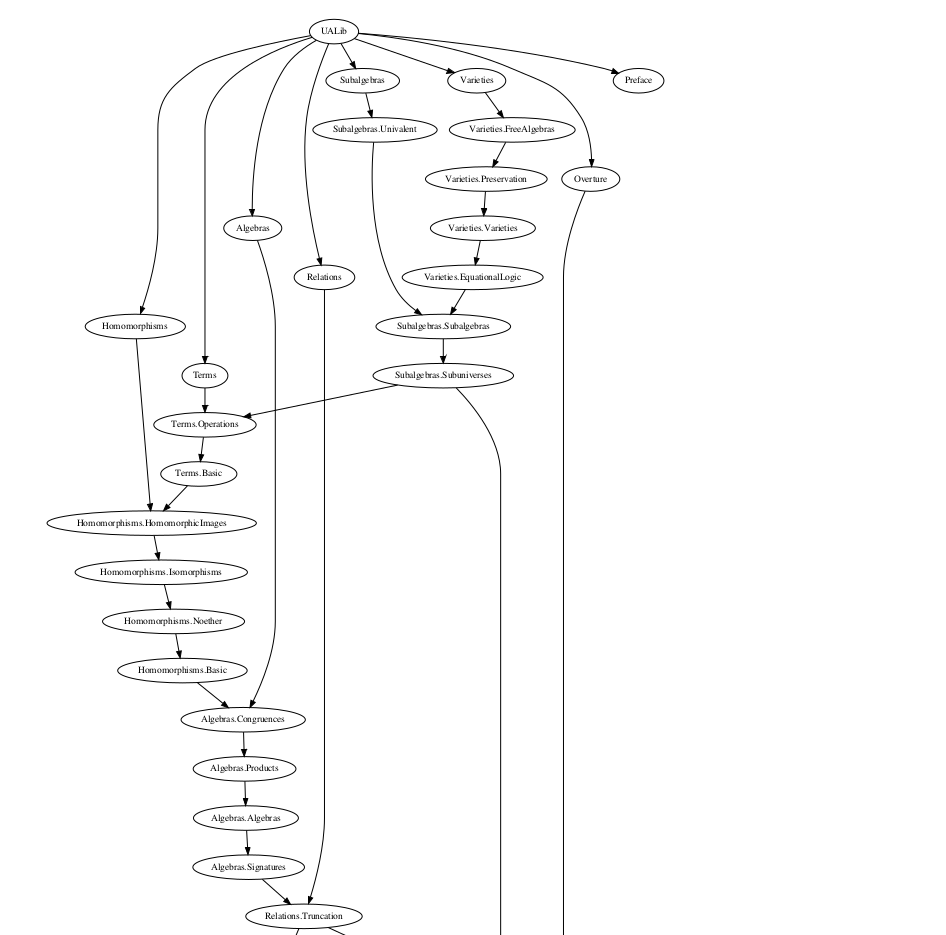
\includegraphics[scale=0.65]{ualib-graph-top.png}

% \newpage

% ~\hskip-2.5cm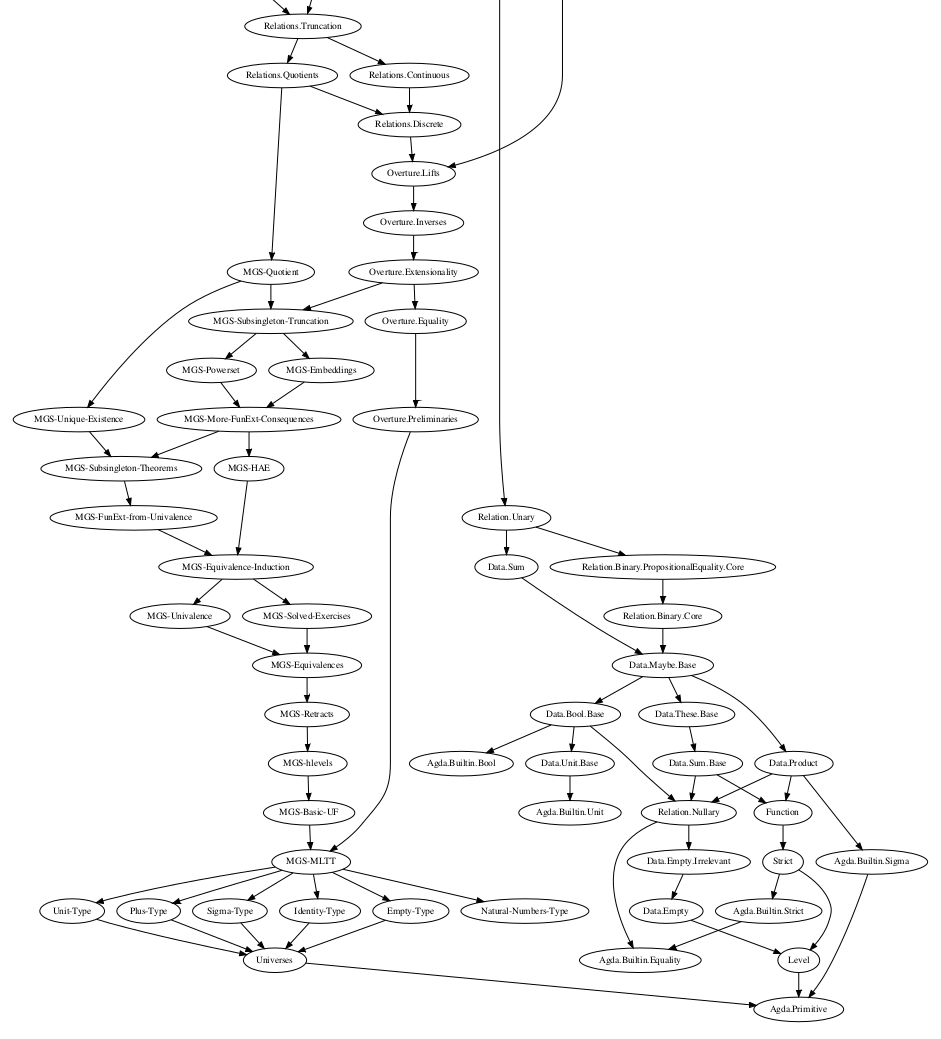
\includegraphics[scale=0.55]{ualib-graph-bot.png}


%% \section{Some Components of the Type Topology Library}
%% Here we collect some of the components from the \typetopology library that we used above but did not have space to discuss.  They are collected here for the reader's convenience and to keep the paper somewhat self-contained.

%% \begin{code}
\>[0]\AgdaFunction{transport}%
\>[1275I]\AgdaSymbol{:}\AgdaSpace{}%
\AgdaSymbol{\{}\AgdaBound{X}\AgdaSpace{}%
\AgdaSymbol{:}\AgdaSpace{}%
\AgdaGeneralizable{𝓤}\AgdaSpace{}%
\AgdaOperator{\AgdaFunction{̇}}\AgdaSpace{}%
\AgdaSymbol{\}}\AgdaSpace{}%
\AgdaSymbol{(}\AgdaBound{A}\AgdaSpace{}%
\AgdaSymbol{:}\AgdaSpace{}%
\AgdaBound{X}\AgdaSpace{}%
\AgdaSymbol{→}\AgdaSpace{}%
\AgdaGeneralizable{𝓥}\AgdaSpace{}%
\AgdaOperator{\AgdaFunction{̇}}\AgdaSpace{}%
\AgdaSymbol{)}\AgdaSpace{}%
\AgdaSymbol{\{}\AgdaBound{x}\AgdaSpace{}%
\AgdaBound{y}\AgdaSpace{}%
\AgdaSymbol{:}\AgdaSpace{}%
\AgdaBound{X}\AgdaSymbol{\}}\<%
\\
\>[.][@{}l@{}]\<[1275I]%
\>[10]\AgdaSymbol{→}\AgdaSpace{}%
\AgdaBound{x}\AgdaSpace{}%
\AgdaOperator{\AgdaDatatype{≡}}\AgdaSpace{}%
\AgdaBound{y}\AgdaSpace{}%
\AgdaSymbol{→}\AgdaSpace{}%
\AgdaBound{A}\AgdaSpace{}%
\AgdaBound{x}\AgdaSpace{}%
\AgdaSymbol{→}\AgdaSpace{}%
\AgdaBound{A}\AgdaSpace{}%
\AgdaBound{y}\<%
\\
%
\\[\AgdaEmptyExtraSkip]%
\>[0]\AgdaFunction{transport}\AgdaSpace{}%
\AgdaBound{A}\AgdaSpace{}%
\AgdaSymbol{(}\AgdaInductiveConstructor{refl}\AgdaSpace{}%
\AgdaBound{x}\AgdaSymbol{)}\AgdaSpace{}%
\AgdaSymbol{=}\AgdaSpace{}%
\AgdaFunction{𝑖𝑑}\AgdaSpace{}%
\AgdaSymbol{(}\AgdaBound{A}\AgdaSpace{}%
\AgdaBound{x}\AgdaSymbol{)}\<%
\end{code}
\scpad
\begin{code}
  \>[0]\AgdaFunction{to-Σ-≡}%
\>[1596I]\AgdaSymbol{:}\AgdaSpace{}%
\AgdaSymbol{\{}\AgdaBound{X}\AgdaSpace{}%
\AgdaSymbol{:}\AgdaSpace{}%
\AgdaGeneralizable{𝓤}\AgdaSpace{}%
\AgdaOperator{\AgdaFunction{̇}}\AgdaSpace{}%
\AgdaSymbol{\}}\AgdaSpace{}%
\AgdaSymbol{\{}\AgdaBound{A}\AgdaSpace{}%
\AgdaSymbol{:}\AgdaSpace{}%
\AgdaBound{X}\AgdaSpace{}%
\AgdaSymbol{→}\AgdaSpace{}%
\AgdaGeneralizable{𝓥}\AgdaSpace{}%
\AgdaOperator{\AgdaFunction{̇}}\AgdaSpace{}%
\AgdaSymbol{\}}\AgdaSpace{}%
\AgdaSymbol{\{}\AgdaBound{σ}\AgdaSpace{}%
\AgdaBound{τ}\AgdaSpace{}%
\AgdaSymbol{:}\AgdaSpace{}%
\AgdaRecord{Σ}\AgdaSpace{}%
\AgdaBound{A}\AgdaSymbol{\}}\<%
\\
\>[.][@{}l@{}]\<[1596I]%
\>[7]\AgdaSymbol{→}\AgdaSpace{}%
\AgdaSymbol{(}\AgdaFunction{Σ}\AgdaSpace{}%
\AgdaBound{p}\AgdaSpace{}%
\AgdaFunction{꞉}\AgdaSpace{}%
\AgdaFunction{pr₁}\AgdaSpace{}%
\AgdaBound{σ}\AgdaSpace{}%
\AgdaOperator{\AgdaDatatype{≡}}\AgdaSpace{}%
\AgdaFunction{pr₁}\AgdaSpace{}%
\AgdaBound{τ}\AgdaSpace{}%
\AgdaFunction{,}\AgdaSpace{}%
\AgdaFunction{transport}\AgdaSpace{}%
\AgdaBound{A}\AgdaSpace{}%
\AgdaBound{p}\AgdaSpace{}%
\AgdaSymbol{(}\AgdaFunction{pr₂}\AgdaSpace{}%
\AgdaBound{σ}\AgdaSymbol{)}\AgdaSpace{}%
\AgdaOperator{\AgdaDatatype{≡}}\AgdaSpace{}%
\AgdaFunction{pr₂}\AgdaSpace{}%
\AgdaBound{τ}\AgdaSymbol{)}\<%
\\
%
\>[7]\AgdaSymbol{→}\AgdaSpace{}%
\AgdaBound{σ}\AgdaSpace{}%
\AgdaOperator{\AgdaDatatype{≡}}\AgdaSpace{}%
\AgdaBound{τ}\<%
\\
%
\\[\AgdaEmptyExtraSkip]%
\>[0]\AgdaFunction{to-Σ-≡}\AgdaSpace{}%
\AgdaSymbol{(}\AgdaInductiveConstructor{refl}\AgdaSpace{}%
\AgdaBound{x}\AgdaSpace{}%
\AgdaOperator{\AgdaInductiveConstructor{,}}\AgdaSpace{}%
\AgdaInductiveConstructor{refl}\AgdaSpace{}%
\AgdaBound{a}\AgdaSymbol{)}\AgdaSpace{}%
\AgdaSymbol{=}\AgdaSpace{}%
\AgdaInductiveConstructor{refl}\AgdaSpace{}%
\AgdaSymbol{(}\AgdaBound{x}\AgdaSpace{}%
\AgdaOperator{\AgdaInductiveConstructor{,}}\AgdaSpace{}%
\AgdaBound{a}\AgdaSymbol{)}\<%
\end{code}


\subsubsection{Dependent function extensionality}\label{dependent-function-extensionality}

dfunext : ∀ 𝓤 𝓥 → (𝓤 ⊔ 𝓥)⁺ ̇
dfunext 𝓤 𝓥 = {X : 𝓤 ̇ } {A : X → 𝓥 ̇ } {f g : Π A} → f ∼ g → f ≡ g

global-dfunext : 𝓤ω
global-dfunext = ∀ {𝓤 𝓥} → dfunext 𝓤 𝓥

happly : {X : 𝓤 ̇ } {A : X → 𝓥 ̇ } (f g : Π A) → f ≡ g → f ∼ g
happly f g p x = ap (λ - → - x) p

Extensionality for dependent function types is defined as follows.
\ccpad
\begin{code}%
\>[0]\AgdaFunction{dep-extensionality}\AgdaSpace{}%
\AgdaSymbol{:}\AgdaSpace{}%
\AgdaSymbol{∀}\AgdaSpace{}%
\AgdaBound{𝓤}\AgdaSpace{}%
\AgdaBound{𝓦}\AgdaSpace{}%
\AgdaSymbol{→}\AgdaSpace{}%
\AgdaBound{𝓤}\AgdaSpace{}%
\AgdaOperator{\AgdaPrimitive{⁺}}\AgdaSpace{}%
\AgdaOperator{\AgdaPrimitive{⊔}}\AgdaSpace{}%
\AgdaBound{𝓦}\AgdaSpace{}%
\AgdaOperator{\AgdaPrimitive{⁺}}\AgdaSpace{}%
\AgdaOperator{\AgdaFunction{̇}}\<%
\\
\>[0]\AgdaFunction{dep-extensionality}\AgdaSpace{}%
\AgdaBound{𝓤}\AgdaSpace{}%
\AgdaBound{𝓦}\AgdaSpace{}%
\AgdaSymbol{=}\AgdaSpace{}%
\AgdaSymbol{\{}\AgdaBound{A}\AgdaSpace{}%
\AgdaSymbol{:}\AgdaSpace{}%
\AgdaBound{𝓤}\AgdaSpace{}%
\AgdaOperator{\AgdaFunction{̇}}\AgdaSpace{}%
\AgdaSymbol{\}}\AgdaSpace{}%
\AgdaSymbol{\{}\AgdaBound{B}\AgdaSpace{}%
\AgdaSymbol{:}\AgdaSpace{}%
\AgdaBound{A}\AgdaSpace{}%
\AgdaSymbol{→}\AgdaSpace{}%
\AgdaBound{𝓦}\AgdaSpace{}%
\AgdaOperator{\AgdaFunction{̇}}\AgdaSpace{}%
\AgdaSymbol{\}}\<%
\\
\>[0][@{}l@{\AgdaIndent{0}}]%
\>[2]\AgdaSymbol{\{}\AgdaBound{f}\AgdaSpace{}%
\AgdaBound{g}\AgdaSpace{}%
\AgdaSymbol{:}\AgdaSpace{}%
\AgdaSymbol{∀(}\AgdaBound{x}\AgdaSpace{}%
\AgdaSymbol{:}\AgdaSpace{}%
\AgdaBound{A}\AgdaSymbol{)}\AgdaSpace{}%
\AgdaSymbol{→}\AgdaSpace{}%
\AgdaBound{B}\AgdaSpace{}%
\AgdaBound{x}\AgdaSymbol{\}}\AgdaSpace{}%
\AgdaSymbol{→}%
\>[28]\AgdaBound{f}\AgdaSpace{}%
\AgdaOperator{\AgdaFunction{∼}}\AgdaSpace{}%
\AgdaBound{g}%
\>[35]\AgdaSymbol{→}%
\>[38]\AgdaBound{f}\AgdaSpace{}%
\AgdaOperator{\AgdaDatatype{≡}}\AgdaSpace{}%
\AgdaBound{g}\<%
\end{code}
\ccpad
Sometimes we need extensionality principles that work at all universe levels, and Agda is capable of expressing such principles, which belong to the special 𝓤ω type, as follows:
\ccpad
\begin{code}%
\>[0]\AgdaFunction{∀-extensionality}\AgdaSpace{}%
\AgdaSymbol{:}\AgdaSpace{}%
\AgdaPrimitive{𝓤ω}\<%
\\
\>[0]\AgdaFunction{∀-extensionality}\AgdaSpace{}%
\AgdaSymbol{=}\AgdaSpace{}%
\AgdaSymbol{∀}%
\>[22]\AgdaSymbol{\{}\AgdaBound{𝓤}\AgdaSpace{}%
\AgdaBound{𝓥}\AgdaSymbol{\}}\AgdaSpace{}%
\AgdaSymbol{→}\AgdaSpace{}%
\AgdaFunction{extensionality}\AgdaSpace{}%
\AgdaBound{𝓤}\AgdaSpace{}%
\AgdaBound{𝓥}\<%
\\
%
\\[\AgdaEmptyExtraSkip]%
\>[0]\AgdaFunction{∀-dep-extensionality}\AgdaSpace{}%
\AgdaSymbol{:}\AgdaSpace{}%
\AgdaPrimitive{𝓤ω}\<%
\\
\>[0]\AgdaFunction{∀-dep-extensionality}\AgdaSpace{}%
\AgdaSymbol{=}\AgdaSpace{}%
\AgdaSymbol{∀}\AgdaSpace{}%
\AgdaSymbol{\{}\AgdaBound{𝓤}\AgdaSpace{}%
\AgdaBound{𝓥}\AgdaSymbol{\}}\AgdaSpace{}%
\AgdaSymbol{→}\AgdaSpace{}%
\AgdaFunction{dep-extensionality}\AgdaSpace{}%
\AgdaBound{𝓤}\AgdaSpace{}%
\AgdaBound{𝓥}\<%
\end{code}
\ccpad
More details about the 𝓤ω type are available at \href{https://agda.readthedocs.io/en/latest/language/universe-levels.html#expressions-of-kind-set}{agda.readthedocs.io}.
\ccpad
\begin{code}%
\>[0]\AgdaFunction{extensionality-lemma}\AgdaSpace{}%
\AgdaSymbol{:}%
\>[119I]\AgdaSymbol{∀}\AgdaSpace{}%
\AgdaSymbol{\{}\AgdaBound{𝓘}\AgdaSpace{}%
\AgdaBound{𝓤}\AgdaSpace{}%
\AgdaBound{𝓥}\AgdaSpace{}%
\AgdaBound{𝓣}\AgdaSymbol{\}}\AgdaSpace{}%
\AgdaSymbol{→}\<%
\\
\>[.][@{}l@{}]\<[119I]%
\>[23]\AgdaSymbol{\{}\AgdaBound{I}\AgdaSpace{}%
\AgdaSymbol{:}\AgdaSpace{}%
\AgdaBound{𝓘}\AgdaSpace{}%
\AgdaOperator{\AgdaFunction{̇}}\AgdaSpace{}%
\AgdaSymbol{\}\{}\AgdaBound{X}\AgdaSpace{}%
\AgdaSymbol{:}\AgdaSpace{}%
\AgdaBound{𝓤}\AgdaSpace{}%
\AgdaOperator{\AgdaFunction{̇}}\AgdaSpace{}%
\AgdaSymbol{\}\{}\AgdaBound{A}\AgdaSpace{}%
\AgdaSymbol{:}\AgdaSpace{}%
\AgdaBound{I}\AgdaSpace{}%
\AgdaSymbol{→}\AgdaSpace{}%
\AgdaBound{𝓥}\AgdaSpace{}%
\AgdaOperator{\AgdaFunction{̇}}\AgdaSpace{}%
\AgdaSymbol{\}}\<%
\\
%
\>[23]\AgdaSymbol{(}\AgdaBound{p}\AgdaSpace{}%
\AgdaBound{q}\AgdaSpace{}%
\AgdaSymbol{:}\AgdaSpace{}%
\AgdaSymbol{(}\AgdaBound{i}\AgdaSpace{}%
\AgdaSymbol{:}\AgdaSpace{}%
\AgdaBound{I}\AgdaSymbol{)}\AgdaSpace{}%
\AgdaSymbol{→}\AgdaSpace{}%
\AgdaSymbol{(}\AgdaBound{X}\AgdaSpace{}%
\AgdaSymbol{→}\AgdaSpace{}%
\AgdaBound{A}\AgdaSpace{}%
\AgdaBound{i}\AgdaSymbol{)}\AgdaSpace{}%
\AgdaSymbol{→}\AgdaSpace{}%
\AgdaBound{𝓣}\AgdaSpace{}%
\AgdaOperator{\AgdaFunction{̇}}\AgdaSpace{}%
\AgdaSymbol{)}\<%
\\
%
\>[23]\AgdaSymbol{(}\AgdaBound{args}\AgdaSpace{}%
\AgdaSymbol{:}\AgdaSpace{}%
\AgdaBound{X}\AgdaSpace{}%
\AgdaSymbol{→}\AgdaSpace{}%
\AgdaSymbol{(}\AgdaFunction{Π}\AgdaSpace{}%
\AgdaBound{A}\AgdaSymbol{))}\<%
\\
\>[0][@{}l@{\AgdaIndent{0}}]%
\>[1]\AgdaSymbol{→}%
\>[23]\AgdaBound{p}\AgdaSpace{}%
\AgdaOperator{\AgdaDatatype{≡}}\AgdaSpace{}%
\AgdaBound{q}\<%
\\
\>[1][@{}l@{\AgdaIndent{0}}]%
\>[23]\AgdaComment{-------------------------------------------------}\<%
\\
\>[0][@{}l@{\AgdaIndent{0}}]%
\>[1]\AgdaSymbol{→}%
\>[23]\AgdaSymbol{(λ}\AgdaSpace{}%
\AgdaBound{i}\AgdaSpace{}%
\AgdaSymbol{→}\AgdaSpace{}%
\AgdaSymbol{(}\AgdaBound{p}\AgdaSpace{}%
\AgdaBound{i}\AgdaSymbol{)(λ}\AgdaSpace{}%
\AgdaBound{x}\AgdaSpace{}%
\AgdaSymbol{→}\AgdaSpace{}%
\AgdaBound{args}\AgdaSpace{}%
\AgdaBound{x}\AgdaSpace{}%
\AgdaBound{i}\AgdaSymbol{))}\AgdaSpace{}%
\AgdaOperator{\AgdaDatatype{≡}}\AgdaSpace{}%
\AgdaSymbol{(λ}\AgdaSpace{}%
\AgdaBound{i}\AgdaSpace{}%
\AgdaSymbol{→}\AgdaSpace{}%
\AgdaSymbol{(}\AgdaBound{q}\AgdaSpace{}%
\AgdaBound{i}\AgdaSymbol{)(λ}\AgdaSpace{}%
\AgdaBound{x}\AgdaSpace{}%
\AgdaSymbol{→}\AgdaSpace{}%
\AgdaBound{args}\AgdaSpace{}%
\AgdaBound{x}\AgdaSpace{}%
\AgdaBound{i}\AgdaSymbol{))}\<%
\\
%
\\[\AgdaEmptyExtraSkip]%
\>[0]\AgdaFunction{extensionality-lemma}\AgdaSpace{}%
\AgdaBound{p}\AgdaSpace{}%
\AgdaBound{q}\AgdaSpace{}%
\AgdaBound{args}\AgdaSpace{}%
\AgdaBound{p≡q}\AgdaSpace{}%
\AgdaSymbol{=}\<%
\\
\>[0][@{}l@{\AgdaIndent{0}}]%
\>[1]\AgdaFunction{ap}\AgdaSpace{}%
\AgdaSymbol{(λ}\AgdaSpace{}%
\AgdaBound{-}\AgdaSpace{}%
\AgdaSymbol{→}\AgdaSpace{}%
\AgdaSymbol{λ}\AgdaSpace{}%
\AgdaBound{i}\AgdaSpace{}%
\AgdaSymbol{→}\AgdaSpace{}%
\AgdaSymbol{(}\AgdaBound{-}\AgdaSpace{}%
\AgdaBound{i}\AgdaSymbol{)}\AgdaSpace{}%
\AgdaSymbol{(λ}\AgdaSpace{}%
\AgdaBound{x}\AgdaSpace{}%
\AgdaSymbol{→}\AgdaSpace{}%
\AgdaBound{args}\AgdaSpace{}%
\AgdaBound{x}\AgdaSpace{}%
\AgdaBound{i}\AgdaSymbol{))}\AgdaSpace{}%
\AgdaBound{p≡q}\<%
\end{code}






%%%%%%%%%%%%%%%%%%%%%%%%%%%%%%%%%%%%%%%%%%%%%%%%%%%%%%%%%%%%%%%%%%%%%%%%%%%
\end{document} %%%%%%%%%%%%%%%%%%%%%%%%%%%%%%%%%%%%%%%%%%%%%%%%%%%%%%%%%%%%
%%%%%%%%%%%%%%%%%%%%%%%%%%%%%%%%%%%%%%%%%%%%%%%%%%%%%%%%%%%%%%%%%%%%%%%%%%%

